% Arquivo LaTeX de exemplo de dissertação/tese a ser apresentada à CPG do IME-USP
%
% Criação: Jesús P. Mena-Chalco
% Revisão: Fabio Kon e Paulo Feofiloff
% Adaptação para UTF8, biblatex e outras melhorias: Nelson Lago
%
% Except where otherwise indicated, these files are distributed under
% the MIT Licence. The example text, which includes the tutorial and
% examples as well as the explanatory comments in the source, are
% available under the Creative Commons Attribution International
% Licence, v4.0 (CC-BY 4.0) - https://creativecommons.org/licenses/by/4.0/


%%%%%%%%%%%%%%%%%%%%%%%%%%%%%%%%%%%%%%%%%%%%%%%%%%%%%%%%%%%%%%%%%%%%%%%%%%%%%%%%
%%%%%%%%%%%%%%%%%%%%%%%%%%%%%%% PREÂMBULO LaTeX %%%%%%%%%%%%%%%%%%%%%%%%%%%%%%%%
%%%%%%%%%%%%%%%%%%%%%%%%%%%%%%%%%%%%%%%%%%%%%%%%%%%%%%%%%%%%%%%%%%%%%%%%%%%%%%%%

% A opção twoside (frente-e-verso) significa que a aparência das páginas pares
% e ímpares pode ser diferente. Por exemplo, as margens podem ser diferentes ou
% os números de página podem aparecer à direita ou à esquerda alternadamente.
% Mas nada impede que você crie um documento "só frente" e, ao imprimir, faça
% a impressão frente-e-verso.
%
% Aqui também definimos a língua padrão do documento
% (a última da lista) e línguas adicionais.
%\documentclass[12pt,twoside,brazilian,english]{book}
\documentclass[12pt,twoside,english,brazilian]{book}

% Ao invés de definir o tamanho das margens, vamos definir os tamanhos do
% texto, do cabeçalho e do rodapé, e deixamos a package geometry calcular
% o tamanho das margens em função do tamanho do papel. Assim, obtemos o
% mesmo resultado impresso, mas com margens diferentes, se o tamanho do
% papel for diferente.
\usepackage[a4paper]{geometry}

\geometry{
  textwidth=152mm,
  hmarginratio=12:17, % 24:34 -> com papel A4, 24mm + 152mm + 34mm = 210mm
  textheight=237mm,
  vmarginratio=8:7, % 32:28 -> com papel A4, 32mm + 237mm + 28mm = 297mm
  headsep=11mm, % distância entre a base do cabeçalho e o texto
  headheight=21mm, % qualquer medida grande o suficiente, p.ex., top - headsep
  footskip=10mm,
  marginpar=20mm,
  marginparsep=5mm,
}

% Vários pacotes e opções de configuração genéricos; para personalizar o
% resultado, modifique estes arquivos.
%%%%%%%%%%%%%%%%%%%%%%%%%%%%%%%%%%%%%%%%%%%%%%%%%%%%%%%%%%%%%%%%%%%%%%%%%%%%%%%%
%%%%%%%%%%%%%%%%%%%%%%% CONFIGURAÇÕES E PACOTES BÁSICOS %%%%%%%%%%%%%%%%%%%%%%%%
%%%%%%%%%%%%%%%%%%%%%%%%%%%%%%%%%%%%%%%%%%%%%%%%%%%%%%%%%%%%%%%%%%%%%%%%%%%%%%%%

% Vários comandos auxiliares para o desenvolvimento de packages e classes;
% aqui, usamos em alguns comandos de formatação e condicionais.
\usepackage{etoolbox}
%\RequirePackage{pdftexcmds}
\usepackage{letltxmacro}
%\usepackage{ltxcmds}

% LaTeX 3
\usepackage{expl3}
\usepackage{xparse}

%\usepackage{filehook}

% Detecta se estamos usando pdftex, luatex, xetex etc.
\usepackage{iftex}

%\usepackage{xfp} % Floating-point calculations

\usepackage{regexpatch}

% O projeto LaTeX3 renomeou algumas macros em 2019-03-05 e removeu
% a compatibilidade com os nomes antigos em 2020-07-17 a partir de
% 2021-01-01 (veja o arquivo l3deprecation.dtx e o changelog em
% https://github.com/latex3/latex3/blob/main/l3kernel/CHANGELOG.md).
% Isso afetou a package regexpatch: versões antigas da package não
% funcionam com versões novas de LaTeX e vice-versa. Infelizmente,
% ubuntu 21.04 (hirsute) e debian 11 (bullseye) incluem essas versões
% incompatíveis e, portanto, a package regexpatch não funciona nesses
% ambientes. Talvez fosse possível contornar esse problema com a
% package latexrelease, mas isso afetaria muitos outros recursos.
% Ao invés disso, vamos restaurar manualmente a compatibilidade.
% TODO: remover isto após debian bullseye se tornar obsoleta,
%       provavelmente no final de 2024.
\makeatletter
\ExplSyntaxOn
\@ifpackagelater{regexpatch}{2021/03/21}
  {} % Se regexpatch é "nova", expl3 deve ser também; nada a fazer
  {
    % Talvez o correto seja 2021/01/01, mas na prática o resultado é o mesmo
    \@ifpackagelater{expl3}{2020/07/17}
      {
        % As versões são incompatíveis; vamos recuperar as macros preteridas
        \cs_gset:Npn \token_get_prefix_spec:N { \cs_prefix_spec:N }
        \cs_gset:Npn \token_get_arg_spec:N { \cs_argument_spec:N }
        \cs_gset:Npn \token_get_replacement_spec:N { \cs_replacement_spec:N }
      }
      {} % As duas packages são antigas e, portanto, compatíveis entre si
  }
\ExplSyntaxOff
\makeatother

% Algumas packages dependem de xpatch e tentam carregá-la, causando conflitos
% com regexpatch. Como regexpatch oferece todos os recursos de xpatch (ela
% é uma versão estendida de xpatch, mas ainda considerada experimental), vamos
% fazê-las acreditar que xpatch já foi carregada.
\makeatletter
\@ifpackagelater{regexpatch}{2020/10/06}
    {\expandafter\xdef\csname ver@xpatch.sty\endcsname{2020/03/25}}
    {\expandafter\xdef\csname ver@xpatch.sty\endcsname{2012/10/02}}
\makeatother

% Acrescenta a correção deste bug (contida na release 2018-11-28):
% https://github.com/latex3/latex2e/issues/94 . Se a correção não
% puder ser aplicada, temos uma versão de LaTeX que já a incorpora.
% Esse bug afeta apenas textos em duas colunas.
% TODO: remover após ubuntu 18.04 se tornar obsoleta (abril/2023)
\makeatletter
\patchcmd\@combinedblfloats{\box\@outputbox}{\unvbox\@outputbox}{}{}
\makeatother

% Arithmetic expressions in \set{length,counter} & \addto{length,counter};
% commands \widthof, \heightof, \depthof, \totalheightof, \settototalheight
\usepackage{calc}

% Algumas packages "padrão" da AMS, que são praticamente obrigatórias.
% Algumas delas devem ser carregadas antes de unicode-math ou das
% definições das fontes do documento. É preciso carregar amsthm após
% amsmath para o comando \qedhere funcionar dentro do ambiente align.
\usepackage{amssymb}
\usepackage{amsmath}
\usepackage{amsthm}

% "fontenc" é um parâmetro do NFSS (sistema de gestão de fontes do
% LaTeX; consulte "texdoc fntguide" e "texdoc fontenc"). O default
% é OT1, mas ele tem algumas limitações; a mais importante é que,
% com ele, palavras acentuadas não podem ser hifenizadas. Por
% conta disso, quase todos os documentos LaTeX utilizam o fontenc
% T1. A escolha do fontenc tem consequências para as fontes que
% podem ser usadas com NFSS; hoje em dia T1 tem mais opções de
% qualidade, então não se perde nada em usá-lo. A package fontspec
% (para gestão de fontes usando outro mecanismo, compatível apenas
% com lualatex e xelatex) carrega fontenc automaticamente, mas
% usando outra codificação ("TU" e não "T1"). Ainda assim, é útil
% carregar o fontenc T1 (antes de carregar fontspec!) para o caso
% de alguma fonte "antiga" ser utilizada no documento (embora isso
% não seja recomendado: lualatex e xelatex só são capazes de
% hifenizar palavras acentuadas com o fontenc TU).
\usepackage[T1]{fontenc}

\ifPDFTeX
  % O texto está escrito em utf8.
  \usepackage[utf8]{inputenc}

  % Várias packages que definem as fontes do documento carregam fontaxes,
  % mas carregamos aqui porque, com qualquer fonte, ela permite utilizar
  % small caps + itálico. Algumas raras packages de fontes podem causar
  % conflitos com fontaxes, em geral por utilizarem a package "concorrente"
  % nfssext-cfr.
  %
  % TODO A funcionalidade pela qual faz sentido carregar fontaxes aqui
  %      (small caps + itálico) foi incorporada ao kernel do LaTeX na
  %      versão 2020-02-02, então está em TeXLive 2021. Remover isto
  %      quando arxiv usar TeXLive >= 2021 e ubuntu 20.04 (focal) for
  %      descontinuada (abril de 2025). As packages que precisam de
  %      fontaxes podem continuar a carregá-la sem problemas.
  \usepackage{fontaxes}

  % LaTeX substitui algumas sequências de caracteres, como
  % "fi", "fl" e outras, por caracteres especiais ("ligaduras").
  % Para que seja possível fazer copiar/colar ou buscas por
  % textos contendo essas ligaduras, o arquivo PDF precisa
  % conter uma tabela indicando quais são elas. Com fontes
  % OTF (LuaLaTeX ou XeLaTeX) isso não costuma ser um problema,
  % mas com pdfLaTeX pode ser. Estes dois comandos (que só
  % existem no pdfLaTeX) incluem uma tabela genérica que
  % funciona para a maioria das fontes. Veja a seção 5 de
  % http://www.tug.org/TUGboat/Articles/tb29-1/tb91thanh-fonts.pdf
  % Note que alguns visualizadores de PDF tentam "adivinhar"
  % o conteúdo da tabela quando ela está incompleta ou não
  % existe, então copiar/colar e buscas podem funcionar em
  % alguns visualizadores e em outros não.
  %
  % TODO Isto foi incluído no kernel do LaTeX versão 2021-06-01,
  %      então está em TeXLive 2022. Remover isto quando arxiv
  %      usar TeXLive >= 2022 e ubuntu 22.04 (jammy) for
  %      descontinuada (abril de 2027).
  \input glyphtounicode.tex
  \pdfgentounicode=1
\else
  % Não é preciso carregar inputenc com LuaTeX e XeTeX, pois
  % com eles utf8 é obrigatório.
  \usepackage{fontspec}

  % Ao invés de usar o sistema tradicional de LaTeX para gerir
  % as fontes matemáticas, utiliza as extensões matemáticas do
  % formato otf definidas pela microsoft. Ao ativar esta package
  % o mecanismo tradicional não funciona mais! Há poucas fontes
  % com suporte a unicode-math.
  \usepackage{unicode-math}
\fi

% Acesso a símbolos adicionais, como \textrightarrow, \texteuro etc.,
% disponíveis na maioria das fontes através do fontenc TS1 ou mudando
% momentaneamente para computer modern/latin modern. Raramente útil
% com lualatex/xelatex, mas não causa problemas. Várias packages de
% fontes carregam textcomp, às vezes com opções específicas; assim,
% para evitar problemas, vamos carregá-la no final do preâmbulo para
% o caso de ela não ter sido carregada antes.
%
% TODO A funcionalidade oferecida por textcomp foi incorporada ao kernel
%      do LaTeX na versão 2020-02-02, então está em TeXLive 2021. Remover
%      isto quando arxiv usar TeXLive >= 2021 e ubuntu 20.04 (focal) for
%      descontinuada (abril de 2025). As packages que precisam de textcomp
%      podem continuar a carregá-la sem problemas.
\AtBeginDocument{\usepackage{textcomp}}

% TeXLive 2018 inclui a versão 2.7a da package microtype e a versão
% 1.07 de luatex. Essa combinação faz aparecer um bug:
% https://tex.stackexchange.com/a/476742
% Aqui, aplicamos a solução sugerida, que não tem "contra-indicações".
% TODO: remover após ubuntu 18.04 se tornar obsoleta (abril/2023)
\ifLuaTeX
  \usepackage{luatexbase}
\fi

% microajustes no tamanho das letras, espaçamento etc. para melhorar
% a qualidade visual do resultado.
\usepackage{microtype}

% Alguns "truques" (sujos?) para minimizar over/underfull boxes.
%
% Para fazer um texto justificado, é preciso modificar o tamanho dos espaços
% em cada linha para mais ou para menos em relação ao seu tamanho ideal. Para
% escolher as quebras de linha, TeX vai percorrendo o texto procurando lugares
% possíveis para quebrar as linhas considerando essa flexibilidade mas dentro
% de um certo limite mínimo/máximo. Nesse processo, ele associa a cada possível
% linha o valor *badness*, que é o nível de distorção do tamanho dos espaços
% daquela linha em relação ao ideal, e ignora opções que tenham badness muito
% grande (esse limite é dado por \tolerance). Depois de encontradas todas
% as possíveis quebras de linha e a badness de cada uma, TeX calcula as
% *penalties* das quebras encontradas, que são uma medida de quebras "ruins".
% Por exemplo, na configuração padrão, quebrar uma linha hifenizando uma
% palavra gera uma penalty de 50; já uma quebra que faça a última linha
% do parágrafo ficar sozinha na página seguinte gera uma penalty de 150.
% Finalmente, TeX calcula a "feiúra" de cada possível linha (demerits)
% com base na badness e nas penalties e escolhe a solução que minimiza os
% demerits totais do parágrafo. Os comandos \linebreak e \pagebreak funcionam
% simplesmente acrescentando uma penalty negativa ao lugar desejado para a
% quebra.
%
% Para cada fonte, o espaço entre palavras tem um tamanho ideal, um
% tamanho mínimo e um tamanho máximo (é possível obter os valores com
% \number\fontdimenX\font\relax, veja https://tex.stackexchange.com/q/88991 ).
% TeX nunca reduz um espaço para menos que o mínimo da fonte, mas pode
% aumentá-lo para mais que o máximo. Se os espaços de uma linha ficam
% com o tamanho ideal, a badness da linha é 0; se o tamanho é
% reduzido/aumentado 50% do mínimo/máximo, a badness da linha é 12; se
% o tamanho é reduzido/aumentado para o mínimo/máximo, a badness é 100,
% e assim por diante. O valor máximo possível para badness é 10.000, que
% significa "badness infinita". Como é feito o cálculo: se as medidas
% do espaço definidas pela fonte são "x plus y minus z" e o tamanho
% final do espaço é "x + k*y" ou "x - k*z", a badness é 100*(k^3). Com
% Libertinus corpo 12, os valores são "3pt plus 1.5pt minus .9996pt",
% Então se o espaço tiver sido aumentado para 3.75pt, o fator é 0.5 e
% a badness é 100*(.5^3) = 12.
%
% \tolerance indica a badness máxima que TeX aceita para uma linha; seu valor
% default é 200. Assim, aumentar para, digamos, 300 ou 400, permite que
% TeX escolha parágrafos com maior variação no espaçamento entre as palavras.
% No entanto, no cálculo de demerits, a badness e as penalties de cada linha
% são elevadas ao quadrado, então TeX geralmente prefere escolher outras
% opções no lugar de uma linha com espaçamento ruim. Por exemplo, órfãs/viúvas
% têm demerit de 22.500 e dois hífens seguidos têm demerit de 10.000; já uma
% linha com badness 400 tem demerit 160.000. Portanto, não é surpreendente que
% a maioria dos parágrafos tenha demerits abaixo de 40.000, quase todos abaixo
% de 100.000 e praticamente nenhum acima de 1.000.000. Isso significa que, para
% a grande maioria dos parágrafos, aumentar \tolerance não faz diferença: uma
% linha com badness 400 nunca será efetivamente escolhida se houver qualquer
% outra opção com badness menor. Também fica claro que não há muita diferença
% real entre definir \tolerance como 800 ou 9.999 (a não ser fazer TeX
% trabalhar mais desnecessariamente).
%
% O problema muda de figura se TeX não consegue encontrar uma solução. Isso
% pode acontecer em dois casos: (1) o parágrafo tem ao menos uma linha que não
% pode ser quebrada com badness < 10.000 ou (2) o parágrafo tem ao menos uma
% linha que não pode ser quebrada com badness < tolerance (mas essa badness é
% menor que 10.000).
%
% No primeiro caso, se houver várias possibilidades de linhas que não podem ser
% quebradas, TeX não vai ser capaz de compará-las e escolher a melhor: todas
% têm a badness máxima (10.000) e, portanto, a que gerar menos deméritos no
% restante do parágrafo será a escolhida. Na realidade, no entanto, essas
% linhas *não* são igualmente ruins entre si, o que pode levar TeX a fazer uma
% má escolha. Para evitar isso, TeX tenta novamente aplicando
% \emergencystretch, que "faz de conta" que o tamanho máximo ideal dos espaços
% da linha é maior que o definido na fonte. Isso reduz a badness de todas as
% linhas, o que soa parecido com aumentar \tolerance. Há três diferenças, no
% entanto: (1) essa mudança só afeta os parágrafos que falharam; (2) soluções
% que originalmente teriam badness = 10.000 (e, portanto, seriam vistas como
% equivalentes) podem ser avaliadas e comparadas entre si; e (3) como a badness
% de todas as linhas diminui, a possibilidade de outras linhas que
% originalmente tinham badness alta serem escolhidas aumenta. Esse último ponto
% significa que \emergencystretch pode fazer TeX escolher linhas mais
% espaçadas, fazendo o espaçamento do parágrafo inteiro aumentar e, portanto,
% tornando o resultado mais homogêneo mesmo com uma linha particularmente ruim.
%
% É esse último ponto que justifica o uso de \emergencystretch no segundo caso
% também: apenas aumentar a tolerância, nesse caso, poderia levar TeX a
% diagramar uma linha ruim em meio a um parágrafo bom, enquanto
% \emergencystretch pode fazer TeX aumentar o espaçamento de maneira geral no
% parágrafo, minimizando o contraste da linha problemática com as demais.
% Colocando a questão de outra maneira, aumentar \tolerance para lidar com
% esses parágrafos problemáticos pode fazê-los ter uma linha especialmente
% ruim, enquanto \emergencystretch pode dividir o erro entre várias linhas.
% Assim, definir \tolerance em torno de 800 parece razoável: no caso geral,
% não há diferença e, se um desses casos difíceis não pode ser resolvido com
% uma linha de badness até 800, \emergencystretch deve ser capaz de gerar um
% resultado igual ou melhor.
%
% Penalties & demerits: https://tex.stackexchange.com/a/51264
% Definições (fussy, sloppy etc.): https://tex.stackexchange.com/a/241355
% Mais definições (hfuzz, hbadness etc.): https://tex.stackexchange.com/a/50850
% Donald Arseneau defendendo o uso de \sloppy: https://groups.google.com/d/msg/comp.text.tex/Dhf0xxuQ66E/QTZ7aLYrdQUJ
% Artigo detalhado sobre \emergencystretch: https://www.tug.org/TUGboat/tb38-1/tb118wermuth.pdf
% Esse artigo me leva a crer que algo em torno de 1.5em é suficiente

\tolerance=800
\hyphenpenalty=100 % Default 50; se o texto é em 2 colunas, 50 é melhor
\setlength{\emergencystretch}{1.5em}

% Não gera warnings para Overfull menor que 1pt
\hfuzz=1pt
\vfuzz\hfuzz

% Não gera warnings para Underfull com badness < 1000
\hbadness=1000
\vbadness=1000

% Por padrão, o algoritmo LaTeX para textos não-justificados é (muito) ruim;
% este pacote implementa um algoritmo bem melhor
\usepackage[newcommands]{ragged2e}

% ragged2e funciona porque permite que LaTeX hifenize palavras em textos
% não-justificados quando necessário. No caso de textos centralizados,
% no entanto, isso em geral não é desejável. Assim, newcommands não é
% interessante para \centering e \begin{center}. newcommands também
% causa problemas com legendas se o float correspondente usa \centering
% (o que é muito comum). Assim, vamos voltar \centering e \begin{center}
% à definição padrão.
\let\centering\LaTeXcentering
\let\center\LaTeXcenter
\let\endcenter\endLaTeXcenter

% Com ragged2e e a opção "newcommands", textos curtos não-justificados
% podem gerar warnings sobre "underfull \hbox". Não há razão para pensar
% muito nesses warnings, então melhor desabilitá-los.
% https://tex.stackexchange.com/a/18019
\makeatletter
\gappto{\raggedright}{\hbadness=\@M}
\gappto{\RaggedRight}{\hbadness=\@M}
\gappto{\raggedleft}{\hbadness=\@M}
\gappto{\RaggedLeft}{\hbadness=\@M}
\gappto{\Centering}{\hbadness=\@M} % not \centering
\gappto{\flushleft}{\hbadness=\@M}
\gappto{\FlushLeft}{\hbadness=\@M}
\gappto{\flushright}{\hbadness=\@M}
\gappto{\FlushRight}{\hbadness=\@M}
\gappto{\Center}{\hbadness=\@M} % not \center
\makeatother

% Espaçamento entre linhas configurável (\singlespacing, \onehalfspacing etc.)
\usepackage{setspace}

% LaTeX às vezes coloca notas de rodapé logo após o final do texto da
% página ao invés de no final da página; este pacote evita isso e faz
% notas de rodapé funcionarem corretamente em títulos de seções.
% Esta package deve ser carregada depois de setspace.
\usepackage[stable,bottom]{footmisc}

% Se uma página está vazia, não imprime número de página ou cabeçalho
\usepackage{emptypage}

% hyperref deve preferencialmente ser carregada próximo ao final
% do preâmbulo mas, para o caso de alguma package forçar a sua
% carga antes de executarmos \usepackage explicitamente, vamos
% garantir que estas opções estejam ativas.
\PassOptionsToPackage{
  unicode=true,
  pdfencoding=unicode,
  plainpages=false,
  pdfpagelabels,
  bookmarksopen=true,
  breaklinks=true,
  %hyperfootnotes=false, % polui desnecessariamente com bordercolor
}{hyperref}

% Carrega nomes de cores disponíveis (podem ser usados com hyperref e listings)
\usepackage[hyperref,svgnames,x11names,table]{xcolor}

% LaTeX oferece 2 pares de comandos nativos para mudar textos para caixa
% alta ou baixa: \uppercase ou \lowercase (TeX "puro") e \MakeUppercase
% ou \MakeLowecase (LaTeX), mas esses comandos têm algumas limitações
% (https://tug.org/TUGboat/tb41-1/tb127wright-case.pdf ). Esta package
% define os comandos \MakeTextUppercase e \MakeTextLowercase que resolvem
% isso.
% TODO: quando TeXLive 2023 for a versão mais antiga de LaTeX a que
%       estivermos dando suporte, podemos eliminar a package textcase
%       e usar \MakeUppercase e \MakeLowercase diretamente. A partir
%       dessa versão, essas macros usam \text_[upper|lower]case:n de
%       expl3.
\usepackage{textcase}

% Em documentos frente-e-verso, LaTeX faz o final da página terminar sempre
% no mesmo lugar (exceto no final dos capítulos). Esse comportamento pode ser
% ativado explicitamente com o comando "\flushbottom". Mas se, por alguma
% razão, o volume de texto na página é "pequeno", essa página vai ter espaços
% verticais artificialmente grandes. Uma solução para esse problema é utilizar
% "\raggedbottom" (padrão em documentos que não são frente-e-verso): com essa
% opção, as páginas podem terminar em alturas ligeiramente diferentes. Outra
% opção é corrigir manualmente cada página problemática, por exemplo com o
% comando "\enlargethispage".
%\raggedbottom
\flushbottom

% Por padrão, LaTeX coloca uma espaço aumentado após sinais de pontuação;
% Isso não é tão bom quanto alguns TeX-eiros defendem :) .
% Esta opção desabilita isso e, consequentemente, evita problemas com
% "id est" (i.e.) e "exempli gratia" (e.g.)
\frenchspacing

% Mais recursos para trechos de texto "puro" (tabs, quebras de linha etc.
% não são modificados), além do ambiente "\begin{comment}".
\usepackage{verbatim}

% Durante o processamento, LaTeX procura por arquivos adicionais necessários
% (tanto componentes do próprio LaTeX, como packages e fontes, quanto partes
% do conteúdo em si, como imagens carregadas com \includegraphics ou arquivos
% solicitados com \input ou \include) no diretório de instalação e também
% no diretório atual (ou seja, o diretório do projeto). Assim, normalmente
% é preciso usar caminhos relativos para incluir arquivos de subdiretórios:
% "\input{diretorio/arquivo}". No entanto, há duas limitações:
%
% 1. É necessário dizer "\input{diretorio/arquivo}" mesmo quando o arquivo
%    que contém esse comando já está dentro do subdiretório.
%
% 2. Isso não deve ser usado para packages ("\usepackage{diretorio/package}"),
%    embora na prática funcione.
%
% Há três maneiras recomendadas de resolver esses problemas:
%
% 1. Acrescentando os diretórios desejados ao arquivo texmf.cnf
%
% 2. Acrescentando os diretórios desejados às variáveis de ambiente
%    TEXINPUTS e BSTINPUTS
%
% 3. Colocando os arquivos adicionais na árvore TEXMF (geralmente, no
%    diretório texmf dentro do diretório do usuário).
%
% Essas soluções, no entanto, não podem ser automatizadas por este modelo
% e são um tanto complicadas para usuários menos experientes. Veja mais a
% respeito na seção 5 de "texdoc kpathsea" e em
% https://www.overleaf.com/learn/latex/Articles/An_introduction_to_Kpathsea_and_how_TeX_engines_search_for_files .
%
% A package import pode solucionar o primeiro problema, mas exige o uso
% de outro comando no lugar de \input, então não a usamos aqui.
%\usepackage{import}
%
% Uma solução mais simples é acrescentar os diretórios desejados à macro
% \input@path, originalmente criada para resolver um problema relacionado
% à portabilidade. Seu uso não é normalmente recomendado por razões de
% desempenho, mas no nosso caso (em que adicionamos apenas um diretório
% com poucos arquivos e com máquinas modernas) isso não é um problema. Veja
% https://tex.stackexchange.com/questions/241828/define-path-for-packages-in-the-latex-file-analog-of-inputpath-or-graphicspa#comment705011_241832
\csappto{input@path}{{extras/}}

%%%%%%%%%%%%%%%%%%%%%%%%%%%%%%%%%%%%%%%%%%%%%%%%%%%%%%%%%%%%%%%%%%%%%%%%%%%%%%%%
%%%%%%%%%%%%%%%%%%%%%%%%%%%%%%%%%%% LÍNGUAS %%%%%%%%%%%%%%%%%%%%%%%%%%%%%%%%%%%%
%%%%%%%%%%%%%%%%%%%%%%%%%%%%%%%%%%%%%%%%%%%%%%%%%%%%%%%%%%%%%%%%%%%%%%%%%%%%%%%%

\makeatletter
\ExplSyntaxOn

% We need to have at least some variant of Portuguese and of English
% loaded to generate the abstract/resumo, palavras-chave/keywords etc.
% We will make sure that both languages are present in the class options
% list by adding them if needed. With this, these options become global
% and therefore are seen by all packages (among them, babel).
%
% babel traditionally uses "portuguese", "brazilian", "portuges", or
% "brazil" to support the Portuguese language, using .ldf files. babel
% is also in the process of implementing a new scheme, using .ini
% files, based on the concept of "locales" instead of "languages". This
% mechanism uses the names "portuguese-portugal", "portuguese-brazil",
% "portuguese-pt", "portuguese-br", "portuguese", "brazilian", "pt",
% "pt-PT", and "pt-BR" (i.e., neither "portuges" nor "brazil"). To avoid
% compatibility problems, let's stick with "brazilian" or "portuguese"
% by substituting portuges and brazil if necessary.

\NewDocumentCommand\@IMEportugueseAndEnglish{m}{

  % Make sure any instances of "portuges" and "brazil" are replaced
  % by "portuguese" e "brazilian"; other options are unchanged.
  \seq_gclear_new:N \l_tmpa_seq
  \seq_gclear_new:N \l_tmpb_seq
  \seq_gset_from_clist:Nc \l_tmpa_seq {#1}

  \seq_map_inline:Nn \l_tmpa_seq{
    \def\@tempa{##1}
    \ifstrequal{portuges}{##1}
      {
        \GenericInfo{sbc2019}{}{Substituting~language~portuges~->~portuguese}
        \def\@tempa{portuguese}
      }
      {}
    \ifstrequal{brazil}{##1}
      {
        \GenericInfo{}{Substituting~language~brazil~->~brazilian}
        \def\@tempa{brazilian}
      }
      {}
    \seq_gput_right:NV \l_tmpb_seq {\@tempa}
  }

  % Remove the leftmost duplicates (default is to remove the rightmost ones).
  % Necessary in case the user did "portuges,portuguese", "brazil,brazilian"
  % or some variation: When we substitute the language, we end up with the
  % exact same language twice, which may mess up the main language selection.
  \seq_greverse:N \l_tmpb_seq
  \seq_gremove_duplicates:N \l_tmpb_seq
  \seq_greverse:N \l_tmpb_seq

  % If the user failed to select some variation of English and Portuguese,
  % we add them here. We also remember which ones of portuguese/brazilian,
  % english/american/british etc. were selected.
  \exp_args:Nnx \regex_extract_all:nnNTF
    {\b(portuguese|brazilian)\b}
    {\seq_use:Nn \l_tmpb_seq {,}}
    \l_tmpa_tl
    {
      \tl_reverse:N \l_tmpa_tl
      \xdef\@IMEpt{\tl_head:N \l_tmpa_tl}
    }
    {
      \seq_gput_left:Nn \l_tmpb_seq {brazilian}
      \gdef\@IMEpt{brazilian}
    }

  \exp_args:Nnx \regex_extract_all:nnNTF
    {\b(english|american|USenglish|canadian|british|UKenglish|australian|newzealand)\b}
    {\seq_use:Nn \l_tmpb_seq {,}}
    \l_tmpa_tl
    {
      \tl_reverse:N \l_tmpa_tl
      \xdef\@IMEen{\tl_head:N \l_tmpa_tl}
    }
    {
      \seq_gput_left:Nn \l_tmpb_seq {english}
      \gdef\@IMEen{english}
    }

  \exp_args:Nc \xdef {#1} {\seq_use:Nn \l_tmpb_seq {,}}
}


% https://tex.stackexchange.com/a/43541
% This message is part of a larger thread that discusses some
% limitations of this method, but it is enough for us here.
\def\@getcl@ss#1.cls#2\relax{\def\@currentclass{#1}}
\def\@getclass{\expandafter\@getcl@ss\@filelist\relax}
\@getclass

% The three class option lists we need to update: \@unusedoptionlist,
% \@classoptionslist and one of \opt@book.cls, \opt@article.cls etc.
% according to the current class. Note that beamer.cls (and maybe
% others) does not use \@unusedoptionlist; with it, we incorrectly
% add "english,brazilian" to \@unusedoptionlist, but that does not
% cause problems.
\@IMEportugueseAndEnglish{@unusedoptionlist}
\@IMEportugueseAndEnglish{@classoptionslist}
\@IMEportugueseAndEnglish{opt@\@currentclass .cls}

\ExplSyntaxOff
\makeatother

% Babel permite definir a língua ou línguas usadas no documento e deve
% ser um dos primeiros pacotes a serem carregados. É possível definir
% as línguas como parâmetro aqui, mas já fizemos isso ao carregar a
% classe, no início do documento.
%
% A escolha da língua afeta quatro coisas:
%
% 1. A internacionalização das palavras criadas automaticamente, como
%    "Capítulo/Chapter", "Sumário/Table of Contents" etc. - babel chama
%    essas palavras de "captions";
%
% 2. A hifenização das palavras;
%
% 3. Algumas convenções tipográficas. Por exemplo, em francês é usual
%    acrescentar um espaço antes de caracteres como "?" e "!"; línguas
%    diferentes usam caracteres diferentes para as aspas tipográficas;
%    com algumas línguas asiáticas, pode ser necessário utilizar uma
%    fonte diferente etc.;
%
% 4. Atalhos (shorthands) - algumas línguas definem "atalhos" (shorthands"),
%    ou seja, tratam alguns caracteres como comandos especiais; por exemplo,
%    em francês o espaço que é colocado antes da exclamação funciona porque
%    o caracter "!" é, na verdade, um comando.
%
%%%% MUDANDO A LÍNGUA E HIFENIZAÇÃO %%%%
%
% Cada documento tem uma língua padrão; quando usamos pequenos trechos em
% outra língua, como por exemplo em citações, queremos alterar apenas os
% aspectos 2, 3 e 4; nesse caso, a troca da língua deve ser feita com
% \foreignlanguage{língua}{texto} ou com \begin{otherlanguage*}{língua}.
% Para alterar todos os quatro aspectos, deve-se usar \selectlanguage{língua}
% (que altera a língua padrão a partir desse ponto) ou
% \begin{otherlanguage}{língua}{texto}, que faz a alteração apenas até
% \end{otherlanguage}. Se você quiser apenas desabilitar a hifenização de
% um trecho de texto, pode usar \begin{hyphenrules}{nohyphenation}.
% Finalmente, com \babeltags é possível definir comandos curtos como
% "\textbr" (para "brazilian") que são equivalentes a \foreignlanguage.
%
%%%% PERSONALIZANDO CAPTIONS %%%%
%
% É possível personalizar os captions. Para versões de babel a partir
% de 3.51 (lançada em outubro de 2020), basta fazer
% \setlocalecaption{english}{contents}{Table of Contents}. Com versões
% anteriores, por razões históricas há dois mecanismos para fazer isso,
% então é preciso checar qual deve ser usado para cada língua (veja a
% documentação de babel ou faça um teste). São eles:
%
%   1. \renewcommand\spanishchaptername{Capítulo}
%
%   2. \addto\captionsenglish{\renewcommand\contentsname{Table of Contents}}
%      (este é o mais comum)
%
% Esses métodos valem também para a bibliografia, mas apenas se você
% estiver usando bibtex; com biblatex, que é o padrão neste modelo, é
% melhor usar o comando "\DefineBibliographyStrings" (veja a documentação
% de biblatex).
%
% Quando babel faz uma troca de língua, ele executa \extraslíngua e, se for
% necessário trocar os "captions", \captionslíngua (ou seja, os comandos
% acima modificam \captionslíngua). Então, se você quiser executar algo a
% mais quando uma língua é selecionada, faça \addto\extrasenglish{\blah}.
\usepackage{babel}
\usepackage{iflang}

% Por padrão, LaTeX utiliza maiúsculas no início de cada palavra nestas
% expressões ("Lista de Figuras"); vamos usar maiúsculas apenas na primeira
% palavra.
\addto\captionsbrazilian{%
  \renewcommand\listfigurename{Lista de figuras}%
  \renewcommand\listtablename{Lista de tabelas}%
  \renewcommand\indexname{Índice remissivo}%
}

% Alguns pacotes (tikz, siunitx) usam, além de babel, este pacote como
% auxiliar para a tradução de palavras-chave, como os meses do ano.
\usepackage{translator}

%%%%%%%%%%%%%%%%%%%%%%%%%%%%%%%%%%%%%%%%%%%%%%%%%%%%%%%%%%%%%%%%%%%%%%%%%%%%%%%%
%%%%%%%%%%%%%%%%%%%%%%%%%%%%%%%%%%% FONTE %%%%%%%%%%%%%%%%%%%%%%%%%%%%%%%%%%%%%%
%%%%%%%%%%%%%%%%%%%%%%%%%%%%%%%%%%%%%%%%%%%%%%%%%%%%%%%%%%%%%%%%%%%%%%%%%%%%%%%%

% LaTeX normalmente usa quatro tipos de fonte:
%
% * uma fonte serifada, para o corpo do texto;
% * uma fonte com design similar à anterior, para modo matemático;
% * uma fonte sem serifa, para títulos ou "entidades". Por exemplo, "a classe
%   \textsf{TimeManager} é responsável..." ou "chamamos \textsf{primos} os
%   números que...". Observe que em quase todos os casos desse tipo é mais
%   adequado usar negrito ou itálico;
% * uma fonte "teletype", para trechos de programas.
%
% A escolha de uma família de fontes para o documento normalmente é feita
% carregando uma package específica que, em geral, seleciona as quatro fontes
% de uma vez.
%
% LaTeX usa por default a família de fontes "Computer Modern". Essas fontes
% precisaram ser re-criadas diversas vezes em formatos diferentes, então há
% diversas variantes dela. Com o fontenc OT1 (default "ruim" do LaTeX), a
% versão usada é a BlueSky Computer Modern, que é de boa qualidade, mas com
% os problemas do OT1. Com fontenc T1 (padrão deste modelo e recomendado), o
% LaTeX usa o conjunto "cm-super". Com fontspec (ou seja, com LuaLaTeX e
% XeLaTeX), LaTeX utiliza a versão "Latin Modern". Ao longo do tempo, versões
% diferentes dessas fontes foram recomendadas como "a melhor"; atualmente, a
% melhor opção para usar a família Computer Modern é a versão "Latin Modern".
%
% Você normalmente não precisa lidar com isso, mas pode ser útil saber: O
% mecanismo tradicionalmente usado por LaTeX para gerir fontes é o NFSS
% (veja "texdoc fntguide"). Ele funciona com todas as versões de LaTeX,
% mas só com fontes que foram adaptadas para funcionar com LaTeX. LuaLaTeX
% e XeLaTeX podem usar NFSS mas também são capazes de utilizar um outro
% mecanismo (através da package fontspec), que permite utilizar quaisquer
% fontes instaladas no computador.

\ifPDFTeX
    % Usando pdfLaTeX

    % Ativa Latin Modern como a fonte padrão.
    \usepackage{lmodern}

    % Alguns truques para melhorar a aparência das fontes Latin Modern;
    % eles não funcionam com LuaLaTeX e XeLaTeX.

    % Latin Modern não tem fontes bold + Small Caps, mas cm-super sim;
    % assim, vamos ativar o suporte às fontes cm-super (sem ativá-las
    % como a fonte padrão do documento) e configurar substituições
    % automáticas para que a fonte Latin Modern seja substituída por
    % cm-super quando o texto for bold + Small Caps.
    \usepackage{fix-cm}

    % Com Latin Modern, é preciso incluir substituições para o encoding TS1
    % também por conta dos números oldstyle, porque para inclui-los nas fontes
    % computer modern foi feita uma hack: os dígitos são declarados como sendo
    % os números itálicos da fonte matemática e, portanto, estão no encoding TS1.
    %
    % Primeiro forçamos o LaTeX a carregar a fonte Latin Modern (ou seja, ler
    % o arquivo que inclui "DeclareFontFamily") e, a seguir, definimos a
    % substituição
    \fontencoding{TS1}\fontfamily{lmr}\selectfont
    \DeclareFontShape{TS1}{lmr}{b}{sc}{<->ssub * cmr/bx/n}{}
    \DeclareFontShape{TS1}{lmr}{bx}{sc}{<->ssub * cmr/bx/n}{}

    \fontencoding{T1}\fontfamily{lmr}\selectfont
    \DeclareFontShape{T1}{lmr}{b}{sc}{<->ssub * cmr/bx/sc}{}
    \DeclareFontShape{T1}{lmr}{bx}{sc}{<->ssub * cmr/bx/sc}{}

    % Latin Modern não tem "small caps + itálico", mas tem "small caps + slanted";
    % vamos definir mais uma substituição aqui.
    \fontencoding{T1}\fontfamily{lmr}\selectfont % já feito acima, mas tudo bem
    \DeclareFontShape{T1}{lmr}{m}{scit}{<->ssub * lmr/m/scsl}{}
    \DeclareFontShape{T1}{lmr}{bx}{scit}{<->ssub * lmr/bx/scsl}{}

    % Se fizermos mudanças manuais na fonte Latin Modern, estes comandos podem
    % vir a ser úteis
    %\newcommand\lmodern{%
    %  \renewcommand{\oldstylenums}[1]{{\fontencoding{TS1}\selectfont ##1}}%
    %  \fontfamily{lmr}\selectfont%
    %}
    %
    %\DeclareRobustCommand\textlmodern[1]{%
    %  {\lmodern #1}%
    %}
\else
    % Com LuaLaTex e XeLaTeX, Latin Modern é a fonte padrão. Existem
    % diversas packages e "truques" para melhorar alguns aspectos de
    % Latin Modern, mas eles foram feitos para pdflatex (veja mais
    % acima). Assim, se você pretende usar Latin Modern como a fonte
    % padrão do documento, é melhor usar pdfLaTeX. Deve ser possível
    % implementar essas melhorias com fontspec também, mas este modelo
    % não faz isso, apenas ativamos Small Caps aqui.

    \ifLuaTeX
      % Com LuaTeX, basta indicar o nome de cada fonte; para descobrir
      % o nome "certo", use o comando "otfinfo -i" e veja os itens
      % "preferred family" e "full name"
      \setmainfont{Latin Modern Roman}[
        SmallCapsFont = {LMRomanCaps10-Regular},
        ItalicFeatures = {
          SmallCapsFont = {LMRomanCaps10-Oblique},
        },
        SlantedFont = {LMRomanSlant10-Regular},
        SlantedFeatures = {
          SmallCapsFont = {LMRomanCaps10-Oblique},
          BoldFont = {LMRomanSlant10-Bold}
        },
      ]
    \fi

    \ifXeTeX
      % Com XeTeX, é preciso informar o nome do arquivo de cada fonte.
      \setmainfont{lmroman10-regular.otf}[
        SmallCapsFont = {lmromancaps10-regular.otf},
        ItalicFeatures = {
          SmallCapsFont = {lmromancaps10-oblique.otf},
        },
        SlantedFont = {lmromanslant10-regular.otf},
        SlantedFeatures = {
          SmallCapsFont = {lmromancaps10-oblique.otf},
          BoldFont = {lmromanslant10-bold.otf}
        },
      ]
    \fi
\fi

% Algumas packages mais novas que tratam de fontes funcionam corretamente
% tanto com fontspec (LuaLaTeX/XeLaTeX) quanto com NFSS (qualquer versão
% de LaTeX, mas menos poderoso que fontspec). No entanto, muitas funcionam
% apenas com NFSS. Nesse caso, em LuaLaTeX/XeLaTeX é melhor usar os
% comandos de fontspec, como exemplificado mais abaixo.

% É possível mudar apenas uma das fontes. Em particular, a fonte
% teletype da família Computer Modern foi criada para simular
% as impressoras dos anos 1970/1980. Sendo assim, ela é uma fonte (1)
% com serifas e (2) de espaçamento fixo. Hoje em dia, é mais comum usar
% fontes sem serifa para representar código-fonte. Além disso, ao imprimir,
% é comum adotar fontes que não são de espaçamento fixo para fazer caber
% mais caracteres em uma linha de texto. Algumas opções de fontes para
% esse fim:
%\usepackage{newtxtt} % Não funciona com fontspec (lualatex / xelatex)
%\usepackage{DejaVuSansMono}
% inconsolata é uma boa fonte, mas não tem variante itálico
%\ifPDFTeX
%  \usepackage[narrow]{inconsolata}
%\else
%  \setmonofont{inconsolatan}
%\fi
\usepackage[scale=.85]{sourcecodepro}

% Ao invés da família Computer Modern, é possível usar outras como padrão.
% Uma ótima opção é a libertine, similar (mas não igual) à Times mas com
% suporte a Small Caps e outras qualidades. A fonte teletype da família
% é serifada, então é melhor definir outra; a opção "mono=false" faz
% o pacote não carregar sua própria fonte, mantendo a escolha anterior.
% Versões mais novas de LaTeX oferecem um fork desta fonte, libertinus.
% As packages libertine/libertinus funcionam corretamente com pdfLaTeX,
% LuaLaTeX e XeLaTeX.
% TODO: remover suporte a Libertine no final de 2022
\makeatletter
\IfFileExists{libertinus.sty}
    {
      \usepackage[mono=false]{libertinus}
      % Com LuaLaTeX/XeLaTeX, Libertinus configura também
      % a fonte matemática; aqui só precisamos corrigir \mathit
      \ifLuaTeX
        \setmathfontface\mathit{Libertinus Serif Italic}
      \fi
      \ifXeTeX
        % O nome de arquivo da fonte mudou na versão 2019-04-04
        \@ifpackagelater{libertinus-otf}{2019/04/03}
            {\setmathfontface\mathit{LibertinusSerif-Italic.otf}}
            {\setmathfontface\mathit{libertinusserif-italic.otf}}
      \fi
    }
    {
      % Libertinus não está disponível; vamos usar libertine
      \usepackage[mono=false]{libertine}

      % Com Libertine, é preciso modificar também a fonte
      % matemática, além de \mathit
      \ifLuaTeX
        \setmathfont{Libertinus Math}
        \setmathfontface\mathit{Linux Libertine O Italic}
      \fi

      \ifXeTeX
        \setmathfont{libertinusmath-regular.otf}
        \setmathfontface\mathit{LinLibertine_RI.otf}
      \fi
    }
\makeatother

\ifPDFTeX
  % A família libertine por padrão não define uma fonte matemática
  % específica para pdfLaTeX; uma opção que funciona bem com ela:
  %\usepackage[libertine]{newtxmath}
  % Outra, provavelmente melhor:
  \usepackage{libertinust1math}
\fi

% Ativa apenas a fonte biolinum, que é a fonte sem serifa da família.
%\IfFileExists{libertinus.sty}
%  \usepackage[sans]{libertinus}
%\else
%  \usepackage{biolinum}
%\fi

% Também é possível usar a Times como padrão; nesse caso, a fonte
% sem serifa usualmente é a Helvetica. Mas provavelmente libertine
% é uma opção melhor.
%\ifPDFTeX
%  \usepackage[helvratio=0.95,largesc]{newtxtext}
%  \usepackage{newtxtt} % Fonte teletype
%  \usepackage{newtxmath}
%\else
%  % Clone da fonte Times como fonte principal
%  \setmainfont{TeX Gyre Termes}
%  \setmathfont[Scale=MatchLowercase]{TeX Gyre Termes Math}
%  % TeX Gyre Termes Math tem um bug e não define o caracter
%  % \setminus; Vamos contornar esse problema usando apenas
%  % esse caracter da fonte STIX Two Math
%  \setmathfont[range=\setminus]{STIX Two Math}
%  % Clone da fonte Helvetica como fonte sem serifa
%  \setsansfont{TeX Gyre Heros}
%  % Clone da Courier como fonte teletype, mas provavelmente
%  % é melhor utilizar sourcecodepro
%  %\setmonofont{TeX Gyre Cursor}
%\fi

% Cochineal é outra opção de qualidade; ela define apenas a fonte
% com serifa.
%
% Com NFSS (recomendado no caso de cochineal):
%\usepackage{cochineal}
%\usepackage[cochineal,vvarbb]{newtxmath}
%\usepackage[cal=boondoxo]{mathalfa}
%
% Com fontspec (até a linha "setmathfontface..."):
%
%\setmainfont{Cochineal}[
%  Extension=.otf,
%  UprightFont=*-Roman,
%  ItalicFont=*-Italic,
%  BoldFont=*-Bold,
%  BoldItalicFont=*-BoldItalic,
%  %Numbers={Proportional,OldStyle},
%]
%
%\DeclareRobustCommand{\lfstyle}{\addfontfeatures{Numbers=Lining}}
%\DeclareTextFontCommand{\textlf}{\lfstyle}
%\DeclareRobustCommand{\tlfstyle}{\addfontfeatures{Numbers={Tabular,Lining}}}
%\DeclareTextFontCommand{\texttlf}{\tlfstyle}
%
%% Cochineal não tem uma fonte matemática; com fontspec, provavelmente
%% o melhor a fazer é usar libertinus.
%\setmathfont{Libertinus Math}
%\setmathfontface\mathit{Cochineal-Italic.otf}

% gentium inclui apenas uma fonte serifada, similar a Garamond, que busca
% cobrir todos os caracteres unicode
%\usepackage{gentium}

% LaTeX normalmente funciona com fontes que foram adaptadas para ele, ou
% seja, ele não usa as fontes padrão instaladas no sistema: para usar
% uma fonte é preciso ativar o pacote correspondente, como visto acima.
% É possível escapar dessa limitação e acessar as fontes padrão do sistema
% com XeTeX ou LuaTeX. Com eles, além dos pacotes de fontes "tradicionais",
% pode-se usar o pacote fontspec para usar fontes do sistema.
%\usepackage{fontspec}
%\setmainfont{DejaVu Serif}
%\setmainfont{Charis SIL}
%\setsansfont{DejaVu Sans}
%\setsansfont{Libertinus Sans}[Scale=1.1]
%\setmonofont{DejaVu Sans Mono}

% fontspec oferece vários recursos interessantes para manipular fontes.
% Por exemplo, Garamond é uma fonte clássica; a versão EBGaramond é muito
% boa, mas não possui versões bold e bold-italic; aqui, usamos
% CormorantGaramond ou Gentium para simular a versão bold.
%\setmainfont{EBGaramond12}[
%  Numbers        = {Lining,} ,
%  Scale          = MatchLowercase ,
%  UprightFont    = *-Regular ,
%  ItalicFont     = *-Italic ,
%  BoldFont       = gentiumbasic-bold ,
%  BoldItalicFont = gentiumbasic-bolditalic ,
%%  BoldFont       = CormorantGaramond Bold ,
%%  BoldItalicFont = CormorantGaramond Bold Italic ,
%]
%
%\newfontfamily\garamond{EBGaramond12}[
%  Numbers        = {Lining,} ,
%  Scale          = MatchLowercase ,
%  UprightFont    = *-Regular ,
%  ItalicFont     = *-Italic ,
%  BoldFont       = gentiumbasic-bold ,
%  BoldItalicFont = gentiumbasic-bolditalic ,
%%  BoldFont       = CormorantGaramond Bold ,
%%  BoldItalicFont = CormorantGaramond Bold Italic ,
%]

% Crimson tem Small Caps, mas o recurso é considerado "em construção".
% Vamos utilizar Gentium para Small Caps
%\setmainfont{Crimson}[
%  Numbers           = {Lining,} ,
%  Scale             = MatchLowercase ,
%  UprightFont       = *-Roman ,
%  ItalicFont        = *-Italic ,
%  BoldFont          = *-Bold ,
%  BoldItalicFont    = *-Bold Italic ,
%  SmallCapsFont     = Gentium Plus ,
%  SmallCapsFeatures = {Letters=SmallCaps} ,
%]
%
%\newfontfamily\crimson{Crimson}[
%  Numbers           = {Lining,} ,
%  Scale             = MatchLowercase ,
%  UprightFont       = *-Roman ,
%  ItalicFont        = *-Italic ,
%  BoldFont          = *-Bold ,
%  BoldItalicFont    = *-Bold Italic ,
%  SmallCapsFont     = Gentium Plus ,
%  SmallCapsFeatures = {Letters=SmallCaps} ,
%]

% Com o pacote fontspec, também é possível usar o comando "\fontspec" para
% selecionar uma fonte temporariamente, sem alterar as fontes-padrão do
% documento.

%%%%%%%%%%%%%%%%%%%%%%%%%%%%%%%%%%%%%%%%%%%%%%%%%%%%%%%%%%%%%%%%%%%%%%%%%%%%%%%%
%%%%%%%%%%%%%%%%%%%%%%%%%%%%% FIGURAS / FLOATS %%%%%%%%%%%%%%%%%%%%%%%%%%%%%%%%%
%%%%%%%%%%%%%%%%%%%%%%%%%%%%%%%%%%%%%%%%%%%%%%%%%%%%%%%%%%%%%%%%%%%%%%%%%%%%%%%%

% LaTeX escolhe automaticamente o "melhor" lugar para colocar cada float.
% Por padrão, ele tenta colocá-los no topo da página e depois no pé da
% página; se não tiver sucesso, vai para a página seguinte e recomeça.
% Se esse algoritmo não tiver sucesso "logo", LaTeX cria uma página só
% com floats. É possível modificar esse comportamento com as opções de
% posicionamento: "tp", por exemplo, instrui LaTeX a considerar apenas
% o topo da página ou uma página só de floats (ignorando o pé da página),
% e "htbp" o instrui para tentar "aqui" como a primeira opção. A ordem
% dessas opções não é relevante: dentre as opções disponíveis, LaTeX
% sempre tenta "aqui, topo, pé, página". Os pacotes "float" e "floatrow"
% acrescentam a opção "H", que significa "aqui, incondicionalmente".
%
% A escolha do "melhor" lugar leva em conta os parâmetros abaixo, mas é
% possível ignorá-los com a opção de posicionamento "!". Dado que os
% valores default não são muito bons para floats "grandes" ou documentos
% com muitos floats, é muito comum usar "!" ou "H". No entanto, modificando
% estes parâmetros o algoritmo automático tende a funcionar melhor. Ainda
% assim, vale ler a discussão a respeito na seção "Limitações do LaTeX"
% deste modelo.

% Fração da página que pode ser ocupada por floats no topo. Default: 0.7
\renewcommand{\topfraction}{.8}
% Idem para documentos em colunas e floats que tomam as 2 colunas. Default: 0.7
%\renewcommand{\dbltopfraction}{.7}
% Fração da página que pode ser ocupada por floats no pé. Default: 0.3
%\renewcommand{\bottomfraction}{.3}
% Fração mínima da página que deve conter texto. Default: 0.2
%\renewcommand{\textfraction}{.2}
% Numa página só de floats, fração mínima que deve ser ocupada. Default: 0.5
% floatpagefraction *deve* ser menor que topfraction.
\renewcommand{\floatpagefraction}{.66}
% Idem para documentos em colunas e floats que tomam as 2 colunas. Default: 0.5
\renewcommand{\dblfloatpagefraction}{.66}
% Máximo de floats no topo da página. Default: 2
\setcounter{topnumber}{3}
% Idem para documentos em colunas e floats que tomam as 2 colunas. Default: 2
%\setcounter{dbltopnumber}{2}
% Máximo de floats no pé da página. Default: 1
\setcounter{bottomnumber}{2}
% Máximo de floats por página. Default: 3
\setcounter{totalnumber}{5}

% A package float é amplamente utilizada; ela permite definir novos tipos
% de float e também acrescenta a possibilidade de definir "H" como opção de
% posicionamento do float, que significa "aqui, incondicionalmente". No
% entanto, ela tem algumas fragilidades e não é atualizada desde 2001.
% floatrow é uma versão aprimorada e com mais recursos da package "float",
% mas também não é atualizada desde 2009. Aqui utilizamos alguns recursos
% disponibilizados por ambas e é possível escolher qual delas utilizar.
% Um dos principais recursos dessas packages é permitir a criação de novos
% tipos de float; veja o arquivo source-code.tex para um exemplo.
%\usepackage{float}
\usepackage{floatrow}

% Por padrão, LaTeX prefere colocar floats no topo da página que
% onde eles foram definidos; vamos mudar isso. Este comando depende
% do pacote "floatrow", carregado logo acima.
\floatplacement{table}{htbp}
\floatplacement{figure}{htbp}

% Em alguns casos, um float pode aparecer antes do local do texto em que
% foi definido (ou seja, no topo da página ao invés do meio da página).
% Esta package garante que floats (tabelas e figuras) só apareçam após
% o local no texto em que foram definidos; veja os detalhes em
% https://tex.stackexchange.com/a/297580 . Note que, se o float tem a
% opção "h", normalmente LaTeX *não* coloca o float no topo da página
% atual: se o float não pode ser colocado "here", ele é delegado para
% a página seguinte. Portanto, com a opção "h" flafter em geral não faz
% diferença.
\usepackage{flafter}

% Às vezes um float pode ser adiado por muitas páginas; é possível forçar
% LaTeX a imprimir todos os floats pendentes com o comando \clearpage mas,
% para isso, o usuário deve identificar os casos problemáticos e inserir
% \clearpage manualmente. Esta package acrescenta o comando \FloatBarrier,
% que executa \clearpage apenas se necessário no local em que é chamado.
% "above" e "below" desabilitam a barreira quando os floats estão na mesma
% página. A desvantagem de placeins é que, para funcionar, ela gera quebras
% de página que muitas vezes são inesperadas; em muitos casos, é melhor
% fazer ajustes manualmente.
\usepackage[above,below]{placeins}

% Em documentos com duas colunas, floats normalmente são colocados como
% parte de uma das colunas. No entanto, é possível usar "\begin{figure*}"
% ou "\begin{table*}" para criar floats que ocupam as duas colunas. Floats
% "duplos" desse tipo têm algumas limitações:
%
% 1. Mesmo que haja espaço disponível na página atual, eles são sempre
%    inseridos na página seguinte ao lugar em que foram definidos (então
%    é comum defini-los antes do lugar "certo" para compensar isso)
%
% 2. Eles só podem aparecer no topo da página ou em uma página de floats,
%    ou seja, nunca "here" nem no pé da página.
%
% 3. Em alguns casos, eles podem aparecer fora da ordem em relação aos
%    demais floats do mesmo tipo (o que não acontece com floats "normais")
%
% Esta package:
%
% 1. Soluciona parcialmente o primeiro problema: floats "duplos" podem
%    aparecer na página em que são definidos se sua definição está contida
%    no texto da coluna da esquerda;
%
% 2. Soluciona o segundo problema: floats "duplos" podem aparecer tanto no
%    topo quanto no pé da página. Observe que eles *não* podem aparecer
%    "here" porque isso não faz sentido: a figura interromperia o fluxo
%    do texto da "outra" coluna (ainda assim, as packages midfloat e cuted
%    permitem fazer isso).
%
% 3. Soluciona o terceiro problema.
\usepackage{stfloats}

% Às vezes é interessante utilizar uma imagem mais larga que o texto.
% Por padrão, \centering *não* vai centralizar a imagem corretamente
% nesse caso. Com esta package, podemos acrescentar a opção "center"
% ao comando \includegraphics para resolver esse problema:
% \noindent\includegraphics[width=1.2\textwidth,center]{imagem}.
% A package tem muitos outros recursos também
\usepackage{adjustbox}

% Define o ambiente "\begin{landscape} -- \end{landscape}"; o texto entre
% esses comandos é impresso em modo paisagem, podendo se estender por várias
% páginas. A rotação não inclui os cabeçalhos e rodapés das páginas.
% O principal uso desta package é em conjunto com a package longtable: se
% você precisa mostrar uma tabela muito larga (que precisa ser impressa em
% modo paisagem) e longa (que se estende por várias páginas), use
% "\begin{landscape}" e "\begin{longtable}" em conjunto. Note que o modo
% landscape entra em ação imediatamente, ou seja, "\begin{landscape}" gera
% uma quebra de página no local em que é chamado. Na maioria dos casos, o
% que se quer não é isso, mas sim um "float paisagem"; isso é o que a
% package rotating oferece (veja abaixo).
\usepackage{pdflscape}

% Define dois novos tipos de float: sidewaystable e sidewaysfigure, que
% imprimem a figura ou tabela sozinha em uma página em modo paisagem. Além
% disso, permite girar elementos na página de diversas outras maneiras.
\usepackage[figuresright,clockwise]{rotating}

% Captions com fonte menor, indentação normal, corpo do texto
% negrito e nome do caption itálico
\usepackage[
  font=small,
  format=plain,
  labelfont=bf,up,
  textfont=it,up]{caption}

% Em geral, a package caption é capaz de "adivinhar" se o caption
% está acima ou abaixo da figura/tabela, mas isso não funciona
% corretamente com longtable. Aqui, forçamos a package a considerar
% que os captions ficam abaixo das tabelas.
\captionsetup*[longtable]{position=bottom}

% Sub-figuras (e seus captions) - observe que existe uma package chamada
% "subfigure", mas ela é obsoleta; use esta no seu lugar.
\usepackage{subcaption}

% Permite criar imagens com texto ao redor
%\usepackage{wrapfig}
% Esta é similar, mas me parece uma opção melhor:
%\usepackage{cutwin}

% Permite incorporar um arquivo PDF como uma página adicional. Útil se
% for necessário importar uma imagem ou tabela muito grande ou ainda
% para definir uma capa personalizada.
\usepackage{pdfpages}

% Permite importar figuras. LaTeX "tradicional" só é capaz de trabalhar com
% figuras EPS; hoje em dia não há nenhuma boa razão para usar essa versão.
% Já pdfTeX, XeTeX e LuaTeX podem usar figuras nos formatos PDF, JPG e PNG.
% Em algumas instalações, essas versões conseguem converter automaticamente
% arquivos EPS para PDF, mas não isso é garantido, então é melhor evitar o
% formato EPS.
\usepackage{graphicx}

% Caixas de texto coloridas
%\usepackage{tcolorbox}


%%%%%%%%%%%%%%%%%%%%%%%%%%%%%%%%%%%%%%%%%%%%%%%%%%%%%%%%%%%%%%%%%%%%%%%%%%%%%%%%
%%%%%%%%%%%%%%%%%%%%%%%%%%%%%%%%%% TABELAS %%%%%%%%%%%%%%%%%%%%%%%%%%%%%%%%%%%%%
%%%%%%%%%%%%%%%%%%%%%%%%%%%%%%%%%%%%%%%%%%%%%%%%%%%%%%%%%%%%%%%%%%%%%%%%%%%%%%%%

% Tabelas simples são fáceis de fazer em LaTeX; tabelas com alguma sofisticação
% são trabalhosas, pois é difícil controlar alinhamento, largura das colunas,
% distância entre células etc. Ou seja, é muito comum que a tabela final fique
% "torta". Por isso, em muitos casos, vale mais a pena gerar a tabela em uma
% planilha, como LibreOffice calc ou excel, transformar em PDF e importar como
% figura, especialmente se você quer controlar largura/altura das células
% manualmente etc. No entanto, se você quiser fazer as tabelas em LaTeX para
% garantir a consistência com o tipo e o tamanho das fontes, é possível e o
% resultado é muito bom. Aqui há alguns pacotes que incrementam os recursos de
% tabelas do LaTeX e alguns comandos pré-prontos que podem facilitar um pouco
% seu uso.

% LaTeX por padrão não permite notas de rodapé dentro de tabelas. De maneira
% geral, notas de rodapé em tabelas são consideradas "ruins" em termos de
% tipografia, mas às vezes são necessárias. Se esse é o caso, o recomendado
% é que as notas de rodapé apareçam no "rodapé" da tabela, com numeração
% própria, e não no rodapé da página. Você pode fazer isso com esta package:
\usepackage{threeparttable}
% Formatação personalizada das notas de threeparttable:
\appto{\TPTnoteSettings}{\footnotesize\itshape}
\def\TPTtagStyle{\textit}
% Outra opção é a package ctable, que ainda oferece vários outros
% recursos mas usa uma sintaxe diferente.
%\usepackage{ctable}

% Se você realmente quer notas de rodapé em tabelas que aparecem como as
% demais notas de rodapé (no final da página e mantendo a sequência numérica),
% você pode usar a package abaixo. No entanto, ela não funciona com floats
% duplos (floats que ocupam toda a largura da página em um documento de duas
% colunas) e, em alguns casos, a nota pode desaparecer ou aparecer em uma
% página diferente da tabela (mova o lugar do texto em que ela é definida
% para resolver esse problema).
\usepackage{tablefootnote}

% Por padrão, cada coluna de uma tabela tem a largura do maior texto contido
% nela, ou seja, se uma coluna contém uma célula muito larga, LaTeX não
% força nenhuma quebra de linha e a tabela "estoura" a largura do papel. A
% solução simples, nesses casos, é inserir uma ou mais quebras de linha
% manualmente, o que além de deselegante não é totalmente trivial (é preciso
% usar \makecell).
% Esta package estende o ambiente tabular para permitir definir um tamanho
% fixo para uma ou mais colunas; nesse caso, LaTeX quebra as linhas se uma
% célula é larga demais para a largura definida. Encontrar valores "bons"
% para as larguras das colunas, no entanto, também é um trabalho manual
% um tanto penoso. As packages tabularx e tabulary permitem configurar
% algumas colunas como "largura automática", evitando a necessidade da
% definição manual. Finalmente, ltxtable permite utilizar tabularx e
% longtable juntas. Neste modelo, não usamos tabularx/tabulary, mas você
% pode carregá-las se quiser.
\usepackage{array}

% Permite alinhar os elementos de uma coluna pelo ponto decimal; dê
% preferência à package siunitx (carregada em utils.tex), que também
% oferece esse recurso e muitos outros.
%\usepackage{dcolumn}

% Define tabelas do tipo "longtable", similares a "tabular" mas que podem ser
% divididas em várias páginas. "longtable" também funciona corretamente com
% notas de rodapé. Note que, como uma longtable pode se estender por várias
% páginas, não faz sentido colocá-las em um float "table". Por conta disso,
% longtable define o comando "\caption" internamente.
\usepackage{longtable}

% Permite agregar linhas de tabelas, fazendo colunas "compridas"
\usepackage{multirow}

% Cria comando adicional para possibilitar a inserção de quebras de linha
% em uma célula de tabela, entre outros
\usepackage{makecell}

% Modifica (melhora) o layout default das tabelas e acrescenta os comandos
% \toprule, \bottomrule, \midrule e \cmidrule. Vale muito a pena ler a
% documentação desta package!
\usepackage{booktabs}

% Permite colorir linhas, colunas ou células
\usepackage{colortbl}

% Ao invés de digitar os dados de uma tabela dentro do seu documento,
% você pode fazer LaTeX ler os dados de um arquivo CSV e criar uma
% tabela automaticamente com uma destas duas packages:
%\usepackage{csvsimple}     % mais simples
%\usepackage{pgfplotstable} % mais complexa

% Você também pode se interessar pelo ambiente "tabbing", que permite
% criar tabelas simples com algumas vantagens em relação a "tabular",
% ou por esta package, que permite criar tabulações.
%\usepackage{tabto}

%%%%%%%%%%%%%%%%%%%%%%%%%%%%%%%%%%%%%%%%%%%%%%%%%%%%%%%%%%%%%%%%%%%%%%%%%%%%%%%%
%%%%%%%%%%%%%%% CAPA E PÁGINAS PRELIMINARES (TESE/DISSERTAÇÃO)  %%%%%%%%%%%%%%%%
%%%%%%%%%%%%%%%%%%%%%%%%%%%%%%%%%%%%%%%%%%%%%%%%%%%%%%%%%%%%%%%%%%%%%%%%%%%%%%%%

% Formatação de datas de acordo com a língua
\usepackage[useregional]{datetime2}
\DTMusemodule{brazilian}{portuges}
\DTMnewdatestyle{month-year}{%
  \renewcommand*{\DTMdisplaydate}[4]{##2,\space##1}%
  \renewcommand*{\DTMDisplaydate}{\DTMdisplaydate}%
}

\makeatletter


%%%%%%%%%%%%%%%%%%%%%%%%%%%%%%%%%%%%%%%%%%%%%%%%%%%%%%%%%%%%%%%%%%%%%%%%%%%%%%%%
%%%%%%%%%%%%%%%%%%%%% TEXTOS PADRÃO EM PT E EN PARA A CAPA %%%%%%%%%%%%%%%%%%%%%
%%%%%%%%%%%%%%%%%%%%%%%%%%%%%%%%%%%%%%%%%%%%%%%%%%%%%%%%%%%%%%%%%%%%%%%%%%%%%%%%

% \extrasLANGUAGE vs \captionsLANGUAGE: https://tex.stackexchange.com/a/354197

% Palavras fixas a serem traduzidas
\providecommand\keywordsname{} % Keywords / Palavras-chave
\providecommand\programname{} % Program / Programa
\providecommand\committeename{} % Examining committee / Comissão julgadora
\providecommand\advisorname{} % Advisor / Orientador(a)
\providecommand\coadvisorname{} % Co-advisor / Coorientador(a)
\providecommand\workname{} % Report, Thesis / Tese, Dissertação, Monografia
\providecommand\degreename{} % Masters, Doctorate, Bachelor / Mestrado, Doutorado, Bacharelado
\providecommand\titlename{} % Master, Doctor, Bachelor / Mestre(a), Doutor(a), Bacharel
\providecommand\@assembleLicenseText[1]{O conteúdo deste trabalho
                                        é publicado sob a licença #1}

% Textos longos a serem traduzidos
\providecommand\@coverTCCText{}
\providecommand\@coverQualiText{}
\providecommand\@coverThesisText{}
\providecommand\@institutionBlockText{} % Só para TCC
\providecommand\@provisionalFrontmatterText{}
\providecommand\@finalFrontmatterText{}
\providecommand\@institution{}

% Este não precisa ser traduzido, o texto em inglês não utiliza
\providecommand\@bywhom{%
  \ifdefstring{\@authorGender}{masc}
    {pelo candidato \@author}
    {pela candidata \@author}%
}

%%%%%%%%%% PORTUGUÊS %%%%%%%%%%
\expandafter\addto\csname captions\@IMEpt\endcsname{%
  \DTMrenewdatestyle{month-year}{%
    \renewcommand*{\DTMdisplaydate}[4]
      {\DTMportugesmonthname{##2}\space de\space##1}%
  }%
  \renewcommand\keywordsname{Palavras-chave}%
  \renewcommand\programname{Programa}%
  \renewcommand\committeename{Comissão julgadora}%
  \renewcommand\advisorname{%
    \iftoggle{@tcc}{%
      \ifdefstring{\@advisorGender}{masc}
        {Supervisor}
        {Supervisora}%
    }{%
      \ifdefstring{\@advisorGender}{masc}
        {Orientador}
        {Orientadora}%
    }%
  }%
  \renewcommand\coadvisorname[1]{%
    \iftoggle{@tcc}{%
      \ifcsstring{@coadvisor#1Gender}{masc}
        {Cossupervisor}
        {Cossupervisora}%
    }{%
      \ifcsstring{@coadvisor#1Gender}{masc}
        {Coorientador}
        {Coorientadora}%
    }%
  }%
  \renewcommand\workname{%
    \iftoggle{@tcc}
      {Monografia}
      {\iftoggle{@qualificacao}
        {Exame de Qualificação}
        {\iftoggle{@doutorado}
          {Tese}
          {Dissertação}%
        }%
      }%
  }%
  \renewcommand\degreename{%
    \iftoggle{@doutorado}
      {Doutorado}
      {\iftoggle{@mestrado}
        {Mestrado}
        {\iftoggle{@tcc}
          {Bacharelado}
          {Nível não definido!}%
        }%
      }%
  }%
  \renewcommand\titlename{%
    \iftoggle{@doutorado}
      {\ifdefstring{\@authorGender}{masc}{Doutor}{Doutora}}
      {\iftoggle{@mestrado}
        {\ifdefstring{\@authorGender}{masc}{Mestre}{Mestra}}
        {\iftoggle{@tcc}
          {Bacharel}{Nível não definido!}%
        }%
      }%
  }%
  %
  %
  \renewcommand\@coverTCCText{%
    Monografia Final\vspace{.5\baselineskip}\\
    \@macCDXCIX{} --- Trabalho de\\
    Formatura Supervisionado%
  }%
  \renewcommand\@coverQualiText{%
    Relatório apresentado ao\\
    Instituto de Matemática e Estatística\\
    da Universidade de São Paulo\\
    para exame de qualificação de\\
    \degreename{} em Ciências%
  }%
  \renewcommand\@coverThesisText{%
    \workname{} apresentada ao\\
    Instituto de Matemática e Estatística\\
    da Universidade de São Paulo\\
    para obtenção do título de\\
    \titlename{} em Ciências%
  }%
  \renewcommand\@institutionBlockText{%
    Universidade de São Paulo\\
    Instituto de Matemática e Estatística\\
    Bacharelado em Ciência da Computação%
  }%
  \renewcommand\@provisionalFrontmatterText{%
    \iftoggle{@qualificacao}{%
      Esta é a versão original do texto de qualificação elaborado
      \@bywhom{}, tal como submetido à Comissão Julgadora.%
    }{%
      Esta é a versão original da \MakeTextLowercase{\workname} elaborada
      \@bywhom{}, tal como submetida à Comissão Julgadora.%
    }%
  }%
  \renewcommand\@finalFrontmatterText{%
    Esta versão da \MakeTextLowercase{\workname} contém as correções e alterações
    sugeridas pela Comissão Julgadora durante a defesa da versão
    original do trabalho, realizada em \DTMusedate{@defensedate}.\\[1\baselineskip]
    Uma cópia da versão original está disponível no Instituto de
    Matemática e Estatística da Universidade de São Paulo.%
  }%
  \renewcommand\@institution{%
    Instituto de Matemática e Estatística,
    Universidade de São Paulo%
  }%
  \renewcommand{\@assembleLicenseText}[1]{O conteúdo deste trabalho
                                          é publicado sob a licença #1}%
}


%%%%%%%%%% INGLÊS %%%%%%%%%%
\expandafter\addto\csname captions\@IMEen\endcsname{%
  \DTMrenewdatestyle{month-year}{%
    \renewcommand*{\DTMdisplaydate}[4]
      {\DTMenglishmonthname{##2},\space##1}%
  }%
  \renewcommand\keywordsname{Keywords}%
  \renewcommand\programname{Program}%
  \renewcommand\committeename{Examining Committee}
  \renewcommand\advisorname{%
    \iftoggle{@tcc}{Supervisor}{Advisor}%
  }%
  \renewcommand\coadvisorname[1]{%
    \iftoggle{@tcc}{Co-supervisor}{Coadvisor}%
  }%
  % "Tese" e "dissertação" têm sentido contrário em língua inglesa:
  % http://guides.lib.berkeley.edu/dissertations_theses
  % https://www.grad.ubc.ca/handbook-graduate-supervision/graduate-thesis
  % Como "Thesis" é o nome genérico, vamos usar para mestrado e doutorado
  %
  %%%%%
  %
  % Nomes possíveis para o TCC em inglês:
  %
  % * monograph/monography
  %     usado para trabalho de alto nível de um autor "senior",
  %     então não faz sentido para um trabalho de graduação.
  %
  % * undergraduate thesis / bachelor's thesis
  %     plausível, mas no nosso caso report parece melhor.
  %
  % * senior project / senior thesis / honor thesis
  %     usado para "TCCs" de caráter fortemente acadêmico;
  %     não é o caso aqui.
  %
  % * essay / report
  %     razoável, porque trata-se de um texto/relato
  %     sobre o projeto de TCC.
  \renewcommand\workname{%
    \iftoggle{@tcc}
      {Capstone Project Report}
      {\iftoggle{@qualificacao}
        {Qualifying Exam}
        {Thesis}%
      }%
  }%
  \renewcommand\degreename{%
    \iftoggle{@doutorado}
      {Doctorate}
      {\iftoggle{@mestrado}
        {Master's}
        {\iftoggle{@tcc}
          {Bachelor}
          {Nível não definido!}%
        }%
      }%
  }%
  \renewcommand\titlename{%
    \iftoggle{@doutorado}
      {Doctor}
      {\iftoggle{@mestrado}
        {Master}
        {\iftoggle{@tcc}
          {Bachelor}%
          {Nível não definido!}%
        }%
      }%
  }%
  %
  %
  \renewcommand\@coverTCCText{%
    Final Essay\vspace{.5\baselineskip}\\
    \@macCDXCIX{} --- Capstone Project%
  }%
  \renewcommand\@coverQualiText{%
    Report presented to the\\
    Institute of Mathematics and Statistics\\
    of the University of São Paulo\\
    for the \titlename{} of Science\\
    qualifying examination\\%
  }%
  \renewcommand\@coverThesisText{%
    \workname{} presented to the\\
    Institute of Mathematics and Statistics\\
    of the University of São Paulo\\
    in partial fulfillment\\
    of the requirements\\
    for the degree of\\
    \titlename{} of Science%
  }%
  \renewcommand\@institutionBlockText{%
    University of São Paulo\\
    Institute of Mathematics and Statistics\\
    Bachelor of Computer Science%
  }%
  \renewcommand\@provisionalFrontmatterText{%
    \iftoggle{@qualificacao}{%
      This is the original version of the qualifying text prepared
      by candidate \@author, as submitted to the Examining Committee.%
    }{%
      This is the original version of the \MakeTextLowercase{\workname} prepared
      by candidate \@author, as submitted to the Examining Committee.%
    }%
  }%
  \renewcommand\@finalFrontmatterText{%
    This version of the \MakeTextLowercase{\workname} includes the corrections
    and modifications suggested by the Examining Committee during
    the defense of the original version of the work, which took
    place on \DTMusedate{@defensedate}.\\[1\baselineskip]
    A copy of the original version is available at the Institute of
    Mathematics and Statistics of the University of São Paulo.%
  }%
  \renewcommand\@institution{%
    Institute of Mathematics and Statistics,
    University of São Paulo%
  }%
  \renewcommand{\@assembleLicenseText}[1]{The content of this work is
                                          published under the #1 license}%
}


%%%%%%%%%%%%%%%%%%%%%%%%%%%%%%%%%%%%%%%%%%%%%%%%%%%%%%%%%%%%%%%%%%%%%%%%%%%%%%%%
%%%%%%%%%%%%%%%%%%%%%%% COLETA E DEFINIÇÃO DE METADADOS %%%%%%%%%%%%%%%%%%%%%%%%
%%%%%%%%%%%%%%%%%%%%%%%%%%%%%%%%%%%%%%%%%%%%%%%%%%%%%%%%%%%%%%%%%%%%%%%%%%%%%%%%

\renewcommand\author[2][masc]{
  \gdef\@author{#2}
  \gdef\@authorGender{#1}
  \hypersetup{pdfauthor={\@author}}
}

\NewDocumentCommand{\orientador}{O{masc} m}{
  \gdef\@advisor{#2}
  \gdef\@advisorGender{#1}
}

% Mais de um coorientador é raro, mas acontece
\ExplSyntaxOn
\newcounter{numberOfCoadvisors}
\NewDocumentCommand\coorientador{O{masc} m}{
    \stepcounter{numberOfCoadvisors}
    \tl_gclear_new:c {@coadvisor\Roman{numberOfCoadvisors}}
    \tl_gclear_new:c {@coadvisor\Roman{numberOfCoadvisors}Gender}

    \tl_set:cn {@coadvisor\Roman{numberOfCoadvisors}} {#2}
    \tl_set:cn {@coadvisor\Roman{numberOfCoadvisors}Gender} {#1}
}

\seq_gclear_new:N \@committeeMembers

\newtoggle{@mestrado}
\newtoggle{@doutorado}
\newtoggle{@tcc}
\newtoggle{@qualificacao}
\newtoggle{@finalversion}

% Opções usando LaTeX3 (veja texdoc l3keys).
\keys_define:nn { IME / defense }
  {
    % Chaves à esquerda definem as variáveis à direita
    data .code:n= {\DTMsavedate{@defensedate}{#1}},
    data .value_required:n = true,
    nivel .choice:,
    nivel / mestrado .code:n = {\@mestrado},
    nivel / masters .code:n = {\@mestrado},
    nivel / dissertacao .code:n = {\@mestrado},
    nivel / doutorado .code:n = {\@doutorado},
    nivel / phd .code:n = {\@doutorado},
    nivel / tese .code:n = {\@doutorado},
    nivel / graduacao .code:n = {\@tcc},
    nivel / bachelor .code:n = {\@tcc},
    nivel / tcc .code:n = {\@tcc},
    nivel .value_required:n = true,
    quali .code:n = {\ifstrequal{#1}{true}{\toggletrue{@qualificacao}}{\togglefalse{@qualificacao}}},
    quali .default:n = {true},
    definitiva .code:n = {\ifstrequal{#1}{true}{\toggletrue{@finalversion}}{\togglefalse{@finalversion}}},
    definitiva .default:n = {true},
    provisoria .code:n = {\ifstrequal{#1}{true}{\togglefalse{@finalversion}}{\toggletrue{@finalversion}}},
    provisoria .default:n = {true},
    programa .tl_gset:N = \@program,
    program .value_required:n = true,
    apoio .tl_gset:N = \@financing,
    apoio .value_required:n = true,
    local .tl_gset:N = \@defenselocation,
    local .value_required:n = true,
    direitos .tl_gset:N = \@license,
    direitos .value_required:n = true,
    fichacatalografica .tl_gset:N = \@catalogingData,
    fichacatalografica .value_required:n = true,
    membrobanca .code:n = {\seq_gput_right:Nn \@committeeMembers {#1}},
    membrobanca .value_required:n = true,
  }

\NewDocumentCommand\defesa{+m}{%
  \keys_set:nn {IME/defense}{#1}

  \exp_args:NV \str_case:nnF \@license
    {
      {CC-BY}{\gdef\@license{\@assembleLicenseText{CC~BY~4.0}\\
        \href{https\c_colon_str//creativecommons.org/licenses/by/4.0/}{%
        (Creative~Commons~Attribution~4.0~International~License)}}
        \hypersetup{pdflicenseurl={https://creativecommons.org/licenses/by/4.0/}}
      }

      {CC-BY-NC}{\gdef\@license{\@assembleLicenseText{CC~BY-NC~4.0}\\
        \href{https\c_colon_str//creativecommons.org/licenses/by-nc/4.0/}{%
        (Creative~Commons~Attribution-NonCommercial~4.0~International~License)}}
        \hypersetup{pdflicenseurl={https://creativecommons.org/licenses/by-nc/4.0/}}
      }

      {CC-BY-ND}{\gdef\@license{\@assembleLicenseText{CC~BY-ND~4.0}\\
        \href{https\c_colon_str//creativecommons.org/licenses/by-nd/4.0/}{%
        (Creative~Commons~Attribution-NoDerivatives~4.0~International~License)}}
        \hypersetup{pdflicenseurl={https://creativecommons.org/licenses/by-nc-nd/4.0/}}
      }

      {CC-BY-SA}{\gdef\@license{\@assembleLicenseText{CC~BY-SA~4.0}\\
        \href{https\c_colon_str//creativecommons.org/licenses/by-sa/4.0/}{%
        (Creative~Commons~Attribution-ShareAlike~4.0~International~License)}}
        \hypersetup{pdflicenseurl={https://creativecommons.org/licenses/by-sa/4.0/}}
      }

      {CC-BY-NC-SA}{\gdef\@license{\@assembleLicenseText{CC~BY-NC-SA~4.0}\\
        \href{https\c_colon_str//creativecommons.org/licenses/by-nc-sa/4.0/}{%
        (Creative~Commons~Attribution-NonCommercial-ShareAlike~4.0~International~License)}}
        \hypersetup{pdflicenseurl={https://creativecommons.org/licenses/by-nc-sa/4.0/}}
      }

      {CC-BY-NC-ND}{\gdef\@license{\@assembleLicenseText{CC~BY-NC-ND~4.0}\\
        \href{https\c_colon_str//creativecommons.org/licenses/by-nc-nd/4.0/}{%
        (Creative~Commons~Attribution-NonCommercial-NoDerivatives~4.0~International~License)}}
        \hypersetup{pdflicenseurl={https://creativecommons.org/licenses/by-nc-nd/4.0/}}
      }
    }
    % If there is no match, use the user-supplied text
    {}
}

\seq_gclear_new:N \@seqkeywordspt
\seq_gclear_new:N \@seqkeywordsen
\newcommand*{\palavrachave}[1]{\seq_gput_right:Nn \@seqkeywordspt {#1}}
\newcommand*{\keyword}[1]{\seq_gput_right:Nn \@seqkeywordsen {#1}}

% Na impressão, as palavras-chave são separadas por pontos
\newcommand*{\@keywordspt}{\seq_use:Nn \@seqkeywordspt {.\space}.}
\newcommand*{\@keywordsen}{\seq_use:Nn \@seqkeywordsen {.\space}.}

% Para inclusão nos metadados com hyperxmp, são separadas por vírgulas
\newcommand*{\@commakeywordspt}{\seq_use:Nn \@seqkeywordspt {,}}
\newcommand*{\@commakeywordsen}{\seq_use:Nn \@seqkeywordsen {,}}

\ExplSyntaxOff

\NewDocumentCommand{\@doutorado}{}{
  \toggletrue{@doutorado}
  \togglefalse{@mestrado}
  \togglefalse{@tcc}
}

\NewDocumentCommand{\@mestrado}{}{
  \togglefalse{@doutorado}
  \toggletrue{@mestrado}
  \togglefalse{@tcc}
}

\NewDocumentCommand{\@tcc}{}{
  \togglefalse{@mestrado}
  \togglefalse{@doutorado}
  \toggletrue{@tcc}
}

% Defaults quando o usuário não define alguma dessas variáveis.
% Não podemos usar \title ou \author aqui porque esses comandos
% dependem de hyperref, que ainda não foi carregada.
\providecommand\@author{Autor não definido!}
\orientador{Orientador não definido!}
\DTMsavedate{@defensedate}{1970-01-01}
\providecommand\@program{Programa não definido!}
\providecommand\@financing{}
\providecommand\@defenselocation{Local não definido!}
\providecommand\@license{Direitos não definidos!}
\providecommand\@title{Título não definido!}
\providecommand\@titlept{Título em português não definido!}
\providecommand\@titleen{Título em inglês não definido!}
\providecommand\@resumo{Resumo não definido!}
\providecommand\@abstract{Abstract não definido!}


%%%%%%%%%%%%%%%%%%%%%%%%%%%%%%%%%%%%%%%%%%%%%%%%%%%%%%%%%%%%%%%%%%%%%%%%%%%%%%%%
%%%%%%%%%%%%%%%%%%%%%%%%%%%%%% TÍTULO E SUBTÍTULO %%%%%%%%%%%%%%%%%%%%%%%%%%%%%%
%%%%%%%%%%%%%%%%%%%%%%%%%%%%%%%%%%%%%%%%%%%%%%%%%%%%%%%%%%%%%%%%%%%%%%%%%%%%%%%%

\ExplSyntaxOn

% Opções usando LaTeX3 (veja texdoc l3keys).
\keys_define:nn { IME / title }
  {
    % Chaves à esquerda definem as variáveis à direita
    titlept .tl_gset:N = \@titlept,
    titlept .value_required:n = true,
    titleen .tl_gset:N = \@titleen,
    titleen .value_required:n = true,
    subtitlept .tl_gset:N = \@subtitlept,
    subtitlept .value_required:n = true,
    subtitleen .tl_gset:N = \@subtitleen,
    subtitleen .value_required:n = true,
  }

\RenewDocumentCommand\title{m}{
  \keys_set:nn {IME/title}{#1}

  \bgroup
  % O título deve existir nas duas línguas; o subtítulo é opcional,
  % mas se houver também deve existir nas duas línguas.
  \IfLanguagePatterns{brazilian}
    {
      \global\let\@title\@titlept
      \ifdefvoid{\@subtitlept}
        {}
        {\global\let\@subtitle\@subtitlept}

      \let\@mainlangtitle\@titlept
      \let\@mainlangsubtitle\@subtitlept
      \let\@otherlangtitle\@titleen
      \let\@otherlangsubtitle\@subtitleen
      \def\@otherlangname{en}
    }
    {
      \global\let\@title\@titleen
      \ifdefvoid{\@subtitleen}
        {}
        {\global\let\@subtitle\@subtitleen}

      \let\@mainlangtitle\@titleen
      \let\@mainlangsubtitle\@subtitleen
      \let\@otherlangtitle\@titlept
      \let\@otherlangsubtitle\@subtitlept
      \def\@otherlangname{pt}
    }

  % Insere os metadados XMP no arquivo PDF final.
  % \@IMEremoveLinebreaksEtc está definida em hyperlinks.tex.

  \@IMEremoveLinebreaksEtc{\@mainlangtitle}
  \@IMEremoveLinebreaksEtc{\@mainlangsubtitle}
  \@IMEremoveLinebreaksEtc{\@otherlangtitle}
  \@IMEremoveLinebreaksEtc{\@otherlangsubtitle}

  \hypersetup{
    pdftitle={\@mainlangtitle
              \ifdefvoid{\@mainlangsubtitle}{}{:~\@mainlangsubtitle}%
             },
  }

  \XMPLangAlt{\@otherlangname}{
      pdftitle={\@otherlangtitle
                \ifdefvoid{\@otherlangsubtitle}{}{:~\@otherlangsubtitle}%
               },
  }

  % XMPLangAlt undefines "\do"; this may cause
  % problems with biblatex, but we do not need
  % to worry here because we are in a group.
  % https://github.com/plk/biblatex/issues/1105
  \egroup
}

\ExplSyntaxOff


%%%%%%%%%%%%%%%%%%%%%%%%%%%%%%%%%%%%%%%%%%%%%%%%%%%%%%%%%%%%%%%%%%%%%%%%%%%%%%%%
%%%%%%%%%%%%%%%%%%%%%%%%%%%%%%%%%% DEDICATÓRIA %%%%%%%%%%%%%%%%%%%%%%%%%%%%%%%%%
%%%%%%%%%%%%%%%%%%%%%%%%%%%%%%%%%%%%%%%%%%%%%%%%%%%%%%%%%%%%%%%%%%%%%%%%%%%%%%%%

% A dedicatória vai em uma página separada, sem numeração,
% com o texto alinhado à direita e margens esquerda e
% superior muito grandes. Vamos fazer isso com uma minipage.
\newenvironment{dedicatoria} {
  \hypersetup{pageanchor=false} % Veja comentário em \maketitle

  \if@openright\cleardoublepage\else\clearpage\fi

  \thispagestyle{empty}
  \vspace*{140mm plus 0mm minus 100mm}
  \noindent
  \begin{FlushRight}
     \begin{minipage}[b][100mm][b]{100mm}
       \begin{FlushRight}
         \itshape
} {
       \end{FlushRight}
     \end{minipage}\hspace*{3em}
  \end{FlushRight}
  \vspace*{50mm plus 0mm minus 10mm}
  \if@openright\cleardoublepage\else\clearpage\fi

  \hypersetup{pageanchor=true}
}


%%%%%%%%%%%%%%%%%%%%%%%%%%%%%%%%%%%%%%%%%%%%%%%%%%%%%%%%%%%%%%%%%%%%%%%%%%%%%%%%
%%%%%%%%%%%%%%%%%%%%%%%%%%%%%%%%%%% RESUMO %%%%%%%%%%%%%%%%%%%%%%%%%%%%%%%%%%%%%
%%%%%%%%%%%%%%%%%%%%%%%%%%%%%%%%%%%%%%%%%%%%%%%%%%%%%%%%%%%%%%%%%%%%%%%%%%%%%%%%

% A página de resumo deve existir em português e inglês; ambas as versões
% utilizam o mesmo environment.

\NewDocumentCommand{\resumo}{+m}{%
  \long\gdef\@resumo{#1}%

  \bgroup
  \@IMEremoveLinebreaksEtc{\@resumo}
  \IfLanguagePatterns{brazilian}
    {
      \hypersetup{
        pdfsubject={\@resumo},
        pdfkeywords={\@commakeywordspt},
      }
    }
    {
      \XMPLangAlt{pt}{pdfsubject={\@resumo}}
      % o item "keywords" não pode ser traduzido

      % XMPLangAlt undefines "\do"; this may cause
      % problems with biblatex, but we do not need
      % to worry here because we are in a group.
      % https://github.com/plk/biblatex/issues/1105
    }
  \egroup

  \bgroup\bgroup % Dois grupos aninhados, veja a documentação da package babel
  \expandafter\selectlanguage\expandafter{\@IMEpt}
  \begin{IMEabstract}\@resumo\end{IMEabstract}
  \egroup\egroup
}

\DeclareDocumentCommand{\abstract}{+m}{%
  \long\gdef\@abstract{#1}%

  \bgroup
  \@IMEremoveLinebreaksEtc{\@abstract}
  \IfLanguagePatterns{brazilian}
    {
      \XMPLangAlt{en}{pdfsubject={\@abstract}}
      % o item "keywords" não pode ser traduzido

      % XMPLangAlt undefines "\do"; this may cause
      % problems with biblatex, but we do not need
      % to worry here because we are in a group.
      % https://github.com/plk/biblatex/issues/1105
    }
    {
      \hypersetup{
        pdfsubject={\@abstract},
        pdfkeywords={\@commakeywordsen},
      }
    }
  \egroup

  \bgroup\bgroup % Dois grupos aninhados, veja a documentação da package babel
  \expandafter\selectlanguage\expandafter{\@IMEen}
  \begin{IMEabstract}\@abstract\end{IMEabstract}
  \egroup\egroup
}

\NewDocumentEnvironment{IMEabstract}{} {
  \if@openright\cleardoublepage\else\clearpage\fi
  \thispagestyle{empty}

    \begin{center}\Large\bfseries\abstractname\end{center}

  \vspace*{2em plus 1em minus 1em}

  \footnotesize

  % Esse é o jeito mais simples de mudar as margens de um parágrafo:
  % faz de conta que é uma lista
  \begin{list}{}{\rightmargin 4em \leftmargin 4em}
    \item\@selfReference
  \end{list}

  \vspace*{1em plus 1em minus 0em}
} {
  % Impede uma quebra de página entre esta linha e a próxima, ou seja,
  % entre a última linha do resumo/abstract e as palavras-chave.
  \@afterheading

  \vspace*{1em plus 1em minus .5em}

  \begingroup

      \setlength{\leftmargini}{\widthof{\textbf{\keywordsname:}\quad}}
      \setlength{\labelwidth}{\widthof{\textbf{\keywordsname:}}}
      \setlength{\labelsep}{\widthof{\quad}}

      \begin{description}
        \item[\keywordsname:]\IfLanguagePatterns{brazilian}
                             {\@keywordspt}
                             {\@keywordsen}%
      \end{description}

  \endgroup
}


%%%%%%%%%%%%%%%%%%%%%%%%%%%%%%%%%%%%%%%%%%%%%%%%%%%%%%%%%%%%%%%%%%%%%%%%%%%%%%%%
%%%%%%%%%%%%%%%%%%%%%% IMPRIME A CAPA E A FOLHA DE ROSTO %%%%%%%%%%%%%%%%%%%%%%%
%%%%%%%%%%%%%%%%%%%%%%%%%%%%%%%%%%%%%%%%%%%%%%%%%%%%%%%%%%%%%%%%%%%%%%%%%%%%%%%%

\RenewDocumentCommand\maketitle{}{
  % Embora as páginas iniciais *pareçam* não ter numeração, a numeração
  % existe, só não é impressa. Os comandos \frontmatter, \mainmatter,
  % \pagenumbering etc. reiniciam a contagem de páginas quando os números
  % passam a ser impressos. Isso significa que há mais de uma página com
  % o número "1". O pacote hyperref não lida bem com essa situação, então
  % vamos desabilitar hyperlinks para números de páginas aqui.
  \hypersetup{pageanchor=false}
  \bgroup
  \onehalfspacing

  \@IMEcover
  \iftoggle{@tcc}{}{\@IMEtitlePage}
  \@IMEversoPage

  \egroup
  \if@openright\cleardoublepage\else\clearpage\fi
  \hypersetup{pageanchor=true}
}

% Layout da capa
\NewDocumentCommand{\@IMEcover}{} {
  \cleardoublepage
  \thispagestyle{empty}

  \begin{hyphenrules}{nohyphenation}
      \iftoggle{@tcc}{\@institutionBlock}{}
      \@titleBlock
      \vspace*{\fill}
      \@detailsBlock
  \end{hyphenrules}
}

% Layout para a página de rosto (duas versões, de acordo
% com a Resolução CoPGr 6018 de 13/10/2011)
\NewDocumentCommand{\@IMEtitlePage}{} {
  \if@openright\cleardoublepage\else\clearpage\fi
  \thispagestyle{empty}

  \begin{hyphenrules}{nohyphenation}
      \@titleBlock
      \vspace*{2cm plus 2cm minus 1cm}
      \@versionInfoBlock
      \vspace*{3.5cm plus 3cm minus 3.5cm}
      \iftoggle{@finalversion}{\@committeeBlock}{}
      \vspace*{2cm plus 2cm minus 2cm}
  \end{hyphenrules}
}

\NewDocumentCommand{\@IMEversoPage}{}{
  \clearpage
  \thispagestyle{empty}
  \ifcsvoid{@catalogingData}
    {\vspace*{4cm}}
    {\vspace*{2cm}}

  \begin{list}{}{\rightmargin 3em \leftmargin 3em}
    \onehalfspacing\centering\footnotesize\itshape
    \item\@license
  \end{list}

  \ifcsvoid{@catalogingData} {} {\vspace{\fill}\@catalogingData}

  \vspace{1cm minus 1cm}
}


%%%%%%%%%%%%%%%%%%%%%%%%%%%%%%%%%%%%%%%%%%%%%%%%%%%%%%%%%%%%%%%%%%%%%%%%%%%%%%%%
%%%%%%%%%%%%%%%%%%%%%%%% POSIÇÃO DOS ELEMENTOS NA CAPA %%%%%%%%%%%%%%%%%%%%%%%%%
%%%%%%%%%%%%%%%%%%%%%%%%%%%%%%%%%%%%%%%%%%%%%%%%%%%%%%%%%%%%%%%%%%%%%%%%%%%%%%%%

% O IME usa uma capa padrão de cartolina para todas as teses/dissertações.
% Essa capa tem uma janela recortada por onde se vê o título e o autor do
% trabalho. Ela fica centralizada na página, tem 100m de largura, 60mm de
% altura e começa 47mm abaixo do topo da página. Como o documento já tem
% margens definidas pelo usuário, precisamos calcular quanto precisamos
% acrescentar ou subtrair dessas margens para colocar o título e autor
% na posição exata (na verdade, com uma pequena folga: 49mm abaixo do topo
% da página, 96mm de largura e 56mm de altura).
%
% Para centralizar horizontalmente, poderíamos pensar em usar "\center",
% mas isso não funciona porque ele centraliza o texto em relação à coluna
% de texto, não à página. Assim, como as margens esquerda e direita do
% documento podem ser diferentes, a janela não ficaria na posição correta.
% O que faremos, então, é colocar essa janela em uma minipage e calcular
% a margem esquerda para que essa minipage fique centralizada.
%
% Além disso, outros elementos da capa também não podem ser centralizados
% com "\center", porque eles ficariam desalinhados em relação à janela
% com o título e autor. Vamos colocar esses outros elementos em uma
% minipage também, mas de tamanho diferente da anterior.
%
% Então, precisamos calcular três valores: a margem adicional em relação ao
% topo da página, a margem esquerda da janela com título e autor e a margem
% esquerda para os demais elementos centralizados da página.

\AtEndPreamble{
  % Calcula o valor das margens (após geometry ser carregada)

  % A distância entre o topo da página e o início do texto (fora o cabeçalho)
  % é dada por (1in + \voffset + \headsep + \topmargin + \headheight).
  % Queremos colocar a caixa com o título 49mm abaixo do topo, então:
  \dimgdef\@topTitleBlockMargin{49mm - (1in + \voffset + \headsep + \topmargin + \headheight)}

  % Quando \vspace é usado no início da página, ele não tem efeito; como
  % não é isso que queremos, vamos usar \vspace*. No entanto, \vspace*
  % é implementado inserindo uma \hrule de espessura zero e depois
  % acrescentando o espaço solicitado. O resultado não é exatamente
  % o esperado, pois \topskip, \parskip e \baselineskip interagem com
  % \vspace* de maneira um tanto complexa:
  % https://tex.stackexchange.com/a/247516
  %
  % Aqui, vamos compensar essa diferença. Note que, se a primeira linha
  % da página tivesse um tamanho de fonte especial, seria necessário
  % usar o valor de \baselineskip correspondente a essa fonte. Além
  % disso, definimos espaçamento simples porque o \vspace* mencionado
  % acima é executado com espaçamento simples.
  \bgroup
  \setstretch {\setspace@singlespace}% \singlespacing adds \baselineskip
  \dimgdef\@topTitleBlockMargin{\@topTitleBlockMargin - \baselineskip - \parskip}
  \egroup

  % Queremos colocar a caixa com o título centralizada na página. "\center"
  % centraliza em função da área de texto, não da página inteira, então
  % não podemos usá-lo, pois as margens esquerda e direita podem ser
  % diferentes. A distância entre a borda esquerda/interna do papel e o
  % início do texto é dada por (1in + \hoffset + \oddsidemargin), então:
  \dimgdef\@leftTitleBlockMargin{(\paperwidth - 96mm)/2 - (1in + \hoffset + \oddsidemargin)}
  \dimgdef\@coverLeftMargin{(\paperwidth - 160mm)/2 - (1in + \hoffset + \oddsidemargin)}
}


%%%%%%%%%%%%%%%%%%%%%%%%%%%%%%%%%%%%%%%%%%%%%%%%%%%%%%%%%%%%%%%%%%%%%%%%%%%%%%%%
%%%%%%%%%%%%% OS ELEMENTOS QUE COMPÕEM A CAPA E A FOLHA DE ROSTO %%%%%%%%%%%%%%%
%%%%%%%%%%%%%%%%%%%%%%%%%%%%%%%%%%%%%%%%%%%%%%%%%%%%%%%%%%%%%%%%%%%%%%%%%%%%%%%%

% Com fontspec (ou seja, lualatex/xelatex), o comando \oldstylenums funciona
% com qualquer fonte que tenha suporte a números old-style. Já com pdflatex,
% o comando para escolher números old style depende da fonte em uso. Nesse
% caso, se não soubermos qual a fonte atual (ou seja, não é nem libertine
% nem libertinus), vamos usar latin modern e torcer para o resultado não ser
% muito discrepante do restante do texto.

% 499 = CDXCIX
\@ifpackageloaded{fontspec}
  {\providecommand{\@macCDXCIX}{mac~\oldstylenums{499}}}
  {
    \providecommand{\@macCDXCIX}{{\fontfamily{lmr}\selectfont mac~\oldstylenums{499}}}

    \@ifpackageloaded{libertinus}
      {\renewcommand{\@macCDXCIX}{{\LibertinusSerifOsF mac~499}}}
      {}

    \@ifpackageloaded{libertine}
      {\renewcommand{\@macCDXCIX}{{\libertineOsF mac~499}}}
      {}
  }

\newcommand{\@coverText}{
  \bgroup
  \setstretch{.9}

  \iftoggle{@tcc}
    {\@coverTCCText}
    {\iftoggle{@qualificacao}{\@coverQualiText}{\@coverThesisText}}
  \par
  \egroup
}

\ExplSyntaxOn
\newcounter{@IMEtmpcnt}
\newcommand*{\@coverPeople} {%
  \begin{tabular}{rl}
    \iftoggle{@tcc}{}{\programname : & \@program \tabularnewline}
    \advisorname : & \@advisor \tabularnewline
    \setcounter{@IMEtmpcnt}{0}%
    \int_while_do:nNnn {\value{@IMEtmpcnt}} < {\value{numberOfCoadvisors}} {%
      \stepcounter{@IMEtmpcnt}%
      \coadvisorname{\Roman{@IMEtmpcnt}}: & \csuse{@coadvisor\Roman{@IMEtmpcnt}} \tabularnewline
    }%
  \end{tabular}
}

\ExplSyntaxOff

\newcommand{\@selfReference} {%
  \bgroup
  \IfLanguagePatterns{brazilian}
    {%
      \let\@currlangtitle\@titlept
      \let\@currlangsubtitle\@subtitlept
    }
    {%
      \let\@currlangtitle\@titleen
      \let\@currlangsubtitle\@subtitleen
    }%
  \@IMEremoveLinebreaksEtc{\@currlangtitle}%
  \@IMEremoveLinebreaksEtc{\@currlangsubtitle}%
  \@author.
  \textbf{\@currlangtitle\ifdefvoid{\@currlangsubtitle}{}{: \textit{\@currlangsubtitle}}}.
  \workname{} (\degreename).
  \@institution,
  São Paulo, \DTMfetchyear{@defensedate}.%
  \egroup
}

% Só para TCC
\newcommand{\@institutionBlock}{

    % A posição do quadro de título é fixa em relação à página;
    % a posição deste quadro é definida em função da posição do
    % quadro de título. Assim, primeiro vamos encontrar onde
    % deve começar o quadro do título. Veja os comentários em
    % \@titleBlock para entender o mecanismo.
    \bgroup
    \hfuzz=60pt % Não precisa avisar que estamos invadindo a margem direita aqui

    \setstretch {\setspace@singlespace}% \singlespacing adds \baselineskip

    \vspace*{\@topTitleBlockMargin}
    \ifdeflength{\@normalstrutheight}
      {}
      {\newlength{\@normalstrutheight}}
    \settoheight{\@normalstrutheight}{\strut}
    \vspace{-\@normalstrutheight}

    % Estamos alinhados com o quadro do título do trabalho,
    % mas não é isso que queremos: a parte inferior deste
    % quadro deve ficar 15mm acima do quadro de título e
    % este quadro tem 20mm de altura, então precisamos subir:
    \vspace{-20mm} % Espaço ocupado por este quadro
    \vspace{-15mm} % Espaço entre este quadro e o quadro de título

    \noindent\strut%
    \hspace*{\@coverLeftMargin}%
%    \fbox{%
      \begin{minipage}[t][20mm][s]{160mm}
        \vspace{0pt plus 20mm}

        \centering\large

        \textsc{\@institutionBlockText}

        \vspace{0pt plus 20mm}
      \end{minipage}
%    }% fbox
    \par

    % Agora precisamos voltar o "cursor" para o começo da página
    % para que o quadro de título seja inserido no lugar certo.
    % Para isso, vamos:
    %
    % 1. Chegar novamente ao início do quadro de título e
    %
    % 2. Retroceder o tamanho da margem superior

    % compensa o espaço inserido por \par logo acima
    \vspace{-\parskip}
    \egroup

    % A altura da minipage já compensou o \vspace{-20mm} acima;
    % ainda precisamos compensar o \vspace{-15mm}
    \vspace{15mm}

    % Agora estamos no início do quadro de título, então
    % podemos recuar exatamente o tamanho da margem superior.
    \vspace{-\@topTitleBlockMargin}
}

% O quadro com o título e o autor que deve ser visível
% através da janela na capa.
\NewDocumentCommand{\@titleBlock}{} {

    \bgroup
    \setstretch {\setspace@singlespace}% \singlespacing adds \baselineskip

    % Este espaço coloca o topo da próxima linha
    % na posição que queremos:
    \vspace*{\@topTitleBlockMargin}

    % No entanto, a próxima linha contém apenas
    % uma minipage, e definir o topo de uma linha
    % desse tipo é complicado. Assim, vamos:
    %
    % 1. Acrescentar um \strut a essa linha;
    %
    % 2. mover o baseline dessa linha para o topo do \strut;
    %
    % 3. Alinhar o topo da minipage ao baseline da linha.
    %
    % Sobre alinhamento de minipages:
    % https://en.wikibooks.org/wiki/LaTeX/Boxes

    \ifdeflength{\@normalstrutheight}
      {}
      {\newlength{\@normalstrutheight}}
    \settoheight{\@normalstrutheight}{\strut}
    \vspace{-\@normalstrutheight}

    \noindent\strut
    \hspace*{\@leftTitleBlockMargin}%
%    \fbox{%
      \begin{minipage}[t][56mm][s]{96mm}
          \vspace*{2cm plus 1.5cm minus 1.8cm}

          \centering\large

          \textbf{\@title}

          \vspace{0.3cm plus 0.2cm minus 0.1cm}

          \ifdefvoid{\@subtitle}{}{\textbf{\textit{\@subtitle}}}

          \vspace{1cm plus 1cm minus 0.6cm}

          \@author

          \vspace*{2cm plus 1.5cm minus 1.8cm}
      \end{minipage}%
%    }% fbox
    \par
    \egroup
}

% As demais informações da capa
\NewDocumentCommand{\@detailsBlock}{} {

  \bgroup
  \hfuzz=60pt % Não precisa avisar que estamos invadindo a margem direita aqui
  \onehalfspacing
  \noindent
  \hspace*{\@coverLeftMargin}%
%  \fbox{%
    \begin{minipage}[t][130mm][s]{160mm}
      \begin{center}
        \Large

        \vspace*{0.3cm plus 0.5cm minus 0.3cm}

        \textsc{\@coverText}

        \vspace*{1.5cm plus 0.5cm minus 0.5cm}

        \large\@coverPeople

        \vspace*{2.5cm plus 1cm minus 1cm}

        \normalsize

        \bgroup
        \singlespacing
        \@financing\par
        \egroup

        \vspace*{1cm plus 1cm minus 0.3cm}

        \@defenselocation

        \iftoggle{@tcc}
          {\DTMfetchyear{@defensedate}}
          {\DTMsetdatestyle{month-year}\DTMusedate{@defensedate}}

      \end{center}
    \end{minipage}%
%  }% fbox
  \par
  \egroup
}

% As informações da banca que vão apenas na versão definitiva
% da página de rosto
\ExplSyntaxOn
\NewDocumentCommand{\@committeeBlock}{} {
    \bgroup
    \onehalfspacing
    \begin{minipage}[t][][t]{\textwidth}
      \begin{quote}
        \normalsize\noindent\committeename :\par
        \begin{list}{}
        {
          \setlength{\leftmargin}{0pt}
          \setlength{\itemsep}{.1\baselineskip}
          \setlength{\topsep}{\baselineskip}
        }
          \item[] \seq_use:Nn \@committeeMembers {\item[]}
        \end{list}
      \end{quote}
    \end{minipage}
    \par
    \egroup
}
\ExplSyntaxOff

% A informação sobre a versão provisória ou definitiva
\NewDocumentCommand{\@versionInfoBlock}{} {%
  % As diretrizes dizem que "A natureza do trabalho, o grau pretendido, o
  % nome da instituição a que é submetido e a área de concentração devem
  % ser alinhados a partir do meio da parte impressa da página para a
  % margem direita, tanto na folha de rosto como na folha de avaliação."
  %
  % Assim, queremos alinhar o texto à direita com uma grande margem
  % à esquerda. Uma solução simples é alinhar o texto à direita
  % e inserir uma minipage. Dentro dela, definimos o texto
  % também alinhado à direita.

  \bgroup
  \onehalfspacing
  \begin{FlushRight}
    %\fbox{
      % Margem direita + 80mm de largura significa que a minipage
      % começa mais ou menos no meio da página.
      \begin{minipage}[t][50mm][s]{80mm}
        \begin{FlushRight}
          \normalsize
          \iftoggle{@finalversion}{%
            \@finalFrontmatterText%
          } {%
            \@provisionalFrontmatterText%
          }%
        \end{FlushRight}
        \vspace*{0pt plus 50mm}
      \end{minipage}
      \par
    %} % fbox
  \end{FlushRight}
  \egroup
}


%%%%%%%%%%%%%%%%%%%%%%%%%%%%%%%%%%%%%%%%%%%%%%%%%%%%%%%%%%%%%%%%%%%%%%%%%%%%%%%%
%%%%%%%%%%%%%%%%%%%%%%%%%%%%%% METADADOS XMP %%%%%%%%%%%%%%%%%%%%%%%%%%%%%%%%%%%
%%%%%%%%%%%%%%%%%%%%%%%%%%%%%%%%%%%%%%%%%%%%%%%%%%%%%%%%%%%%%%%%%%%%%%%%%%%%%%%%

% TODO: Com versões recentes de hyperxmp (final de 2020), não é
%       recomendado definir pdflang; no futuro, isto deve ser mudado.
\AtEndPreamble{
\IfLanguagePatterns{brazilian}
  {
    \hypersetup{
      pdflang={pt},
      pdfmetalang={pt},
    }
  }
  {
    \hypersetup{
      pdflang={en},
      pdfmetalang={en},
    }
  }
}


%%%%%%%%%%%%%%%%%%%%%%%%%%%%%%%%%%%%%%%%%%%%%%%%%%%%%%%%%%%%%%%%%%%%%%%%%%%%%%%%
%%%%%%%%%%%%%%%%%%%%%%%%%%%%% SUMÁRIO E SEÇÕES %%%%%%%%%%%%%%%%%%%%%%%%%%%%%%%%%
%%%%%%%%%%%%%%%%%%%%%%%%%%%%%%%%%%%%%%%%%%%%%%%%%%%%%%%%%%%%%%%%%%%%%%%%%%%%%%%%

% titlesec permite definir formatação personalizada de títulos, seções etc.
% Observe que titlesec é incompatível com os comandos refsection
% e refsegment do pacote biblatex!
% Esta package utiliza titlesec e implementa a possibilidade de incluir
% uma imagem no título dos capítulos com o comando \imgchapter (leia
% os comentários no arquivo da package).
\usepackage{imagechapter} % carregado do diretório extras (veja basics.tex)

\makeatother
 % capa, páginas preliminares e alguns detalhes
%%%%%%%%%%%%%%%%%%%%%%%%%%%%%%%%%%%%%%%%%%%%%%%%%%%%%%%%%%%%%%%%%%%%%%%%%%%%%%%%
%%%%%%%%%%%%%%%%%%%%%%% SUMÁRIO, CABEÇALHOS, SEÇÕES %%%%%%%%%%%%%%%%%%%%%%%%%%%%
%%%%%%%%%%%%%%%%%%%%%%%%%%%%%%%%%%%%%%%%%%%%%%%%%%%%%%%%%%%%%%%%%%%%%%%%%%%%%%%%

% Formatação personalizada do sumário, lista de tabelas/figuras etc.
%\usepackage{titletoc}

% titlesec permite definir formatação personalizada de títulos, seções etc.
% Observe que titlesec é incompatível com os comandos refsection
% e refsegment do pacote biblatex!
% Vamos usar titlesec apenas
% para fazer títulos, seções etc. não serem justificados.
\usepackage[raggedright]{titlesec}

% Permite saber o número total de páginas; útil para colocar no
% rodapé algo como "página 3 de 10" com "\thepage\ de \zpageref{LastPage}"
%\usepackage{zref-lastpage,zref-user}

% Permite definir cabeçalhos e rodapés
%\usepackage{fancyhdr}

% Personalização de cabeçalhos e rodapés com o estilo deste modelo
\usepackage{imeusp-headers} % carregado do diretório extras (veja basics.tex)

% biblatex pode ser configurado para inserir a bibliografia no sumário;
% bibtex não oferece essa possibilidade. Com esta package, resolvemos
% esse problema.
\usepackage[nottoc,notlot,notlof]{tocbibind}

% Só olha até o nível 2 (subseções) para gerar o sumário e os
% cabeçalhos, ou seja, não coloca nomes de subsubseções (nível 3)
% no sumário nem nos cabeçalhos.
\setcounter{tocdepth}{2}

% Só numera até o nível 2 (subseções, como 2.3.1), ou seja, não numera
% sub-subseções (como 2.3.1.1). Veja que isso afeta referências
% cruzadas: se você fizer \ref{uma-sub-subsecao} sem que ela seja
% numerada, a referência vai apontar para a seção um nível acima.
\setcounter{secnumdepth}{2}

% Normalmente, o capítulo de introdução não deve ser numerado, mas
% deve aparecer no sumário. Por padrão, LaTeX não oferece uma solução
% para isso, então criamos aqui os comandos \unnumberedchapter,
% \unnumberedsection e \unnumberedsubsection.
\newcommand{\unnumberedchapter}[2][]{
  \ifblank{#1}
    {
      \chapter*{#2}
      \phantomsection
      \addcontentsline{toc}{chapter}{#2}
      \chaptermark{#2}
    }
    {
      \chapter*{#2}
      \phantomsection
      \addcontentsline{toc}{chapter}{#1}
      \chaptermark{#1}
    }
}

\newcommand{\unnumberedsection}[2][]{
  \ifblank{#1}
    {
      \section*{#2}
      \phantomsection
      \addcontentsline{toc}{section}{#2}
      \sectionmark{#2}
    }
    {
      \section*{#2}
      \phantomsection
      \addcontentsline{toc}{section}{#1}
      \sectionmark{#1}
    }
}

\newcommand{\unnumberedsubsection}[2][]{
  \ifblank{#1}
    {
      \subsection*{#2}
      \phantomsection
      \addcontentsline{toc}{subsection}{#2}
    }
    {
      \subsection*{#2}
      \phantomsection
      \addcontentsline{toc}{subsection}{#1}
    }
}


%%%%%%%%%%%%%%%%%%%%%%%%%%%%%%%%%%%%%%%%%%%%%%%%%%%%%%%%%%%%%%%%%%%%%%%%%%%%%%%%
%%%%%%%%%%%%%%%%%%%%%%%%%% ESPAÇAMENTO E ALINHAMENTO %%%%%%%%%%%%%%%%%%%%%%%%%%%
%%%%%%%%%%%%%%%%%%%%%%%%%%%%%%%%%%%%%%%%%%%%%%%%%%%%%%%%%%%%%%%%%%%%%%%%%%%%%%%%

% LaTeX por default segue o estilo americano e não faz a indentação da
% primeira linha do primeiro parágrafo de uma seção; este pacote ativa essa
% indentação, como é o estilo brasileiro
\usepackage{indentfirst}

% A primeira linha de cada parágrafo costuma ter um pequeno recuo para
% tornar mais fácil visualizar onde cada parágrafo começa. Além disso, é
% possível colocar um espaço em branco entre um parágrafo e outro. Esta
% package coloca o espaço em branco e desabilita o recuo; como queremos
% o espaço *e* o recuo, é preciso guardar o valor padrão do recuo e
% redefini-lo depois de carregar a package.
% TODO: depois que ubuntu 18.04 se tornar obsoleta (abril/2023), remover
%       as linhas "oldparindent" e carregar a package com a opção "indent".
\newlength\oldparindent
\setlength\oldparindent\parindent
\usepackage[parfill]{parskip}
\setlength\parindent\oldparindent


%%%%%%%%%%%%%%%%%%%%%%%%%%%%%%%%%%%%%%%%%%%%%%%%%%%%%%%%%%%%%%%%%%%%%%%%%%%%%%%%
%%%%%%%%%%%%%%%%%%%%%%%%%% EPÍGRAFE E NOTAS DE RODAPÉ %%%%%%%%%%%%%%%%%%%%%%%%%%
%%%%%%%%%%%%%%%%%%%%%%%%%%%%%%%%%%%%%%%%%%%%%%%%%%%%%%%%%%%%%%%%%%%%%%%%%%%%%%%%

% O formato padrão do pacote epigraph é bem feinho...
% Outra opção para epígrafes é o pacote quotchap
\usepackage{epigraph}

\setlength\epigraphwidth{.85\textwidth}

% Sem linha entre o texto e o autor
\setlength{\epigraphrule}{0pt}

% Ambiente auxiliar para colocar margem à direita da epígrafe
% (como sempre, o modo mais simples de mudar as margens de um
% pagrágrafo é fazer de conta que é uma lista)
\newenvironment{epShiftLeft}
  {
    \par\begin{list}{}
      {
        \leftmargin 0pt
        \labelwidth 0pt
        \labelsep 0pt
        \itemsep 0pt
        \topsep 0pt
        \partopsep 0pt
        \rightmargin 2em
      }
    \item\FlushRight
  }
  {
    \end{list}
    % O espaço padrão que epigraph coloca entre a citação
    % e o autor é muito pequeno; vamos aumentar um pouco
    \vspace*{.3\baselineskip}
  }

\renewcommand\textflush{epShiftLeft}
\renewcommand\sourceflush{epShiftLeft}

\newcommand{\epigrafe}[2] {%
  \ifstrempty{#2}{
    \epigraph{\itshape #1}{}
  }{
    \epigraph{\itshape #1}{--- #2}
  }
}

% Formato personalizado para as notas de rodapé. Copiado quase
% literalmente do exemplo na documentação das classes-padrão de
% LaTeX2e (texdoc classes). Seria possível fazer algo similar
% usando list{} com um único item usando \@thefnmark como label.

% \footnotesep não é um espaço adicional, mas sim um strut que
% existe no começo de cada nota. É por isso que o valor é "grande"
% (\baselineskip) mas a separação de fato é pequena.
\makeatletter
\renewcommand\@makefntext[1]{%
    \setlength{\footnotesep}{1\baselineskip}%
    \@setpar{%
        \@@par
        \@tempdima = \hsize
        \advance\@tempdima-4pt\relax
        \parshape \@ne 4pt \@tempdima
    }%
    \par
    \parindent 1em\noindent
    \parskip .3\baselineskip
    \hbox to \z@{\hss\@makefnmark\,}#1%
}
\makeatother

% \maketitle redefine as notas de rodapé (\thanks) para usar símbolos
% ao invés de números, mas essa não é a única mudança. \maketitle
% também muda \@makefnmark para que a indicação de nota de rodapé
% não ocupe espaço horizontal (isso é feito com \rlap). Isso é feito
% porque a lista de autores em geral é similar a
% \author{Fulano\thanks{instituição 1}, Ciclano\thanks{instituição 2}}.
% Com essa mudança, a nota aparece acima da vírgula entre os autores.
% Mas isso significa que\maketitle precisa também modificar \@makefntext
% para que esse efeito aconteça apenas na lista de autores e não na
% nota em si. Assim, como criamos um novo formato para as notas de
% rodapé, precisamos mudar o formato em \maketitle também.
\makeatletter
\newcommand\@maketitlemakefntext[1]{%
    \setlength{\footnotesep}{1\baselineskip}%
    \@setpar{%
        \@@par
        \@tempdima = \hsize
        \advance\@tempdima-4pt\relax
        \parshape \@ne 4pt \@tempdima
    }%
    \par
    \parindent 1em\noindent
    \parskip .3\baselineskip
    \hbox to \z@{\hss\@textsuperscript{\normalfont\@thefnmark}\,}#1%
}

\patchcmd\maketitle
  {\long\def\@makefntext}
  {\let\@makefntext\@maketitlemakefntext\long\def\@disabledmakefntext}
  {}{}

\makeatother

%%%%%%%%%%%%%%%%%%%%%%%%%%%%%%%%%%%%%%%%%%%%%%%%%%%%%%%%%%%%%%%%%%%%%%%%%%%%%%%%
%%%%%%%%%%%%%%%%%%%%%%%%%%%%%% ÍNDICE REMISSIVO %%%%%%%%%%%%%%%%%%%%%%%%%%%%%%%%
%%%%%%%%%%%%%%%%%%%%%%%%%%%%%%%%%%%%%%%%%%%%%%%%%%%%%%%%%%%%%%%%%%%%%%%%%%%%%%%%

% Cria índice remissivo. Este pacote precisa ser carregado antes de hyperref.
% A criação do índice remissivo depende de um programa auxiliar, que pode ser
% o "makeindex" (default) ou o xindy. xindy é mais poderoso e lida melhor com
% línguas diferentes e caracteres acentuados, mas o programa não está mais
% sendo mantido e índices criados com xindy não funcionam em conjunto com
% hyperref. Se quiser utilizar xindy mesmo assim, é possível contornar esse
% segundo problema configurando hyperref para *não* gerar hyperlinks no
% índice (mais abaixo) e configurando xindy para que ele gere esses hyperlinks
% por conta própria. Para isso, modifique a chamada ao pacote imakeidx (aqui)
% e altere as opções do pacote hyperref.
\providecommand\theindex{} % evita erros de compilação se a classe não tem index
%\usepackage[xindy]{imakeidx} % usando xindy
\usepackage{imakeidx} % usando makeindex

% Cria o arquivo de configuração para xindy lidar corretamente com hyperlinks.
\begin{filecontents*}{hyperxindy.xdy}
(define-attributes ("emph"))
(markup-locref :open "\hyperpage{" :close "}" :attr "default")
(markup-locref :open "\textbf{\hyperpage{" :close "}}" :attr "textbf")
(markup-locref :open "\textit{\hyperpage{" :close "}}" :attr "textit")
(markup-locref :open "\emph{\hyperpage{" :close "}}" :attr "emph")
\end{filecontents*}

% Cria o arquivo de configuração para makeindex colocar um cabeçalho
% para cada letra do índice.
\begin{filecontents*}{mkidxhead.ist}
headings_flag 1
heading_prefix "{\\bfseries "
heading_suffix "}\\nopagebreak\n"
\end{filecontents*}

% Por padrão, o cabeçalho das páginas do índice é feito em maiúsculas;
% vamos mudar isso e deixar fancyhdr definir a formatação
\indexsetup{
  othercode={\chaptermark{\indexname}},
}

\makeindex[
  noautomatic,
  intoc,
  % Estas opções são usadas por xindy
  % "-C utf8" ou "-M lang/latin/utf8.xdy" são truques para contornar este
  % bug, que existe em outras distribuições tambem:
  % https://bugs.launchpad.net/ubuntu/+source/xindy/+bug/1735439
  % Se "-C utf8" não funcionar, tente "-M lang/latin/utf8.xdy"
  %options=-C utf8 -M hyperxindy.xdy,
  %options=-M lang/latin/utf8.xdy -M hyperxindy.xdy,
  % Estas opções são usadas por makeindex
  options=-s mkidxhead.ist -l -c,
]

\PassOptionsToPackage{
  % hyperref não gera hyperlinks corretos em índices remissivos criados
  % com xindy; assim, é possível desabilitar essa função aqui e gerar os
  % os hyperlinks através da configuração de xindy definida anteriormente.
  % Com makeindex (o default), quem precisa criar os hyperlinks é hyperref.
  %hyperindex=false,
}{hyperref}

%%%%%%%%%%%%%%%%%%%%%%%%%%%%%%%%%%%%%%%%%%%%%%%%%%%%%%%%%%%%%%%%%%%%%%%%%%%%%%%%
%%%%%%%%%%%%%%%%%%%%%%%%%%%%%%% BIBLIOGRAFIA %%%%%%%%%%%%%%%%%%%%%%%%%%%%%%%%%%%
%%%%%%%%%%%%%%%%%%%%%%%%%%%%%%%%%%%%%%%%%%%%%%%%%%%%%%%%%%%%%%%%%%%%%%%%%%%%%%%%

% Tradicionalmente, bibliografias no LaTeX são geradas com uma combinação entre
% LaTeX (muitas vezes usando o pacote natbib) e um programa auxiliar chamado
% bibtex. Nesse esquema, LaTeX e natbib são responsáveis por formatar as
% referências ao longo do texto e a formatação da bibliografia fica por conta
% do programa bibtex. A configuração dessa formatação é feita através de um
% arquivo auxiliar de "estilo", com extensão ".bst". Vários journals etc.
% fornecem o arquivo .bst que corresponde ao formato esperado da bibliografia.
%
% bibtex e natbib funcionam bem e, se você tiver alguma boa razão para usá-los,
% obterá bons resultados. No entanto, bibtex tem dois problemas: não lida
% corretamente com caracteres acentuados (embora, na prática, funcione com
% os caracteres usados em português) e o formato .bst, que define a formatação
% da bibliografia, é complexo e pouco flexível.
%
% Por conta disso, a comunidade está migrando para um novo sistema chamado
% biblatex. No biblatex, as formatações da bibliografia e das citações são
% feitas pelo próprio pacote biblatex, dentro do LaTeX. Assim, é bem mais fácil
% modificar e personalizar o estilo da bibliografia. biblatex usa o mesmo
% formato de arquivo de dados do bibtex (".bib") e, portanto, não é difícil
% migrar de um para o outro. biblatex também usa um programa auxiliar (biber),
% mas não para realizar a formatação da bibliografia. A maior desvantagem de
% biblatex é que ele é significativamente mais lento que bibtex.
%
% Observe que biblatex pode criar bibliografias independentes por capítulo
% ou outras divisões do texto. Normalmente é preciso indicar essas seções
% manualmente, mas as opções "refsection" e "refsegment" fazem biblatex
% identificar cada capítulo/seção/etc como uma nova divisão desse tipo.
% No entanto, refsection e refsegment são incompatíveis com o pacote
% titlesec, mencionado em imeusp-formatting.tex. Se você pretende criar
% bibliografias independentes por seções, há duas soluções: (1) desabilitar
% o pacote titlesec; (2) indicar as seções manualmente.
%
% Algumas dicas de configuração:
% https://tex.stackexchange.com/q/12806
% https://github.com/PaulStanley/biblatex-tutorial/releases

\PassOptionsToPackage{
  natbib=true, % Reconhece a sintaxe de natbib (\citet, \citep)
  hyperref=true, % Ativa o suporte ao pacote hyperref
  % Se um item da bibliografia tem língua definida (com langid), permite
  % hifenizar com base na língua selecionada.
  autolang=hyphen,
  % Inclui, em cada item da bibliografia, links para as páginas onde o
  % item foi citado
  backref=true,
}{biblatex}

% Este arquivo é executado antes de carregarmos biblatex, então precisamos
% adiar a execução deste comando. Não carregamos biblatex neste arquivo
% porque o usuário pode querer modificar o estilo bibliográfico, que é
% definido por um parâmetro na hora da carga da package.
\AtEndPreamble{
  % TODO: remover menção ao bug de atendvi/hyperxmp em 2024
  % Impede que um item da bibliografia seja dividido em duas páginas.
  % À parte a estética, isso contorna este bug, que afeta links na
  % úlima página do trabalho, ou seja, pode afetar a bibliografia
  % (atenddvi pode ser carregada por hyperxmp):
  % https://github.com/ho-tex/atenddvi/issues/1
  \AtBeginBibliography{\interlinepenalty=10000\raggedbottom}
}

\makeatletter
\AtEndPreamble{
  % backrefs só fazem sentido com documentos grandes
  \ifboolexpr{test {\@ifclassloaded{book}} or test {\@ifclassloaded{report}}}
    {}
    {\ExecuteBibliographyOptions{backref=false,}}
}
\makeatother

%%%%%%%%%%%%%%%%%%%%%%%%%%%%%%%%%%%%%%%%%%%%%%%%%%%%%%%%%%%%%%%%%%%%%%%%%%%%%%%%
%%%%%%%%%%%%%%%%%%%%%%%%%% HIPERLINKS E REFERÊNCIAS %%%%%%%%%%%%%%%%%%%%%%%%%%%%
%%%%%%%%%%%%%%%%%%%%%%%%%%%%%%%%%%%%%%%%%%%%%%%%%%%%%%%%%%%%%%%%%%%%%%%%%%%%%%%%

% O comando \ref por padrão mostra apenas o número do elemento a que se
% refere; assim, é preciso escrever "veja a Figura~\ref{grafico}" ou
% "como visto na Seção~\ref{sec:introducao}". Usando o pacote hyperref
% (carregado mais abaixo), esse número é transformado em um hiperlink.
%
% Se você quiser mudar esse comportamento, ative as packages varioref
% e cleveref e também as linhas "labelformat" e "crefname" mais abaixo.
% Nesse caso, você deve escrever apenas "veja a \ref{grafico}" ou
% "como visto na \ref{sec:introducao}" etc. e o nome do elemento será
% gerado automaticamente como hiperlink.
%
% Se, além dessa mudança, você quiser usar os recursos de varioref ou
% cleveref, mantenha as linhas labelformat comentadas e use os comandos
% \vref ou \cref, conforme sua preferência, também sem indicar o nome do
% elemento, que é inserido automaticamente. Vale lembrar que o comando
% \vref de varioref pode causar problemas com hyperref, impedindo a
% geração do PDF final.
%
% ATENÇÃO: varioref, hyperref e cleveref devem ser carregadas nessa ordem!
%\usepackage{varioref}

%\labelformat{figure}{Figura~#1}
%\labelformat{table}{Tabela~#1}
%\labelformat{equation}{Equação~#1}
%% Isto não funciona corretamente com os apêndices; o comando seguinte
%% contorna esse problema
%%\labelformat{chapter}{Capítulo~#1}
%\makeatletter
%\labelformat{chapter}{\@chapapp~#1}
%\makeatother
%\labelformat{section}{Seção~#1}
%\labelformat{subsection}{Seção~#1}
%\labelformat{subsubsection}{Seção~#1}

% Cria hiperlinks para capítulos, seções, \ref's, URLs etc.
\usepackage{hyperref}

\providetoggle{IMEcolorlinks}
\providetoggle{IMEhidelinks}
\newcommand\hidelinks{\toggletrue{IMEhidelinks}}
\newcommand\colorlinks{\toggletrue{IMEcolorlinks}}
\newcommand\nocolorlinks{\togglefalse{IMEcolorlinks}}
\colorlinks
\AtEndPreamble{
  \iftoggle{IMEhidelinks}
    {\hypersetup{hidelinks}}
    {
      \iftoggle{IMEcolorlinks}{
        \hypersetup{
          colorlinks=true, % também desabilita pdfborderstyle
          %citecolor=black,
          %linkcolor=black,
          %urlcolor=black,
          %filecolor=black,
          citecolor=DarkGreen,
          linkcolor=NavyBlue,
          urlcolor=DarkRed,
          filecolor=green,
          anchorcolor=black,
        }
      }{
        \hypersetup{
          colorlinks=false,
          pdfborder={0 0 .6},
          pdfborderstyle={/S/U/W .6},
          urlbordercolor=DodgerBlue,
          citebordercolor=green!30!white,
          linkbordercolor=blue!30!white,
          filebordercolor=green!30!white,
        }
      }
    }
}

%\usepackage[nameinlink,noabbrev,capitalise]{cleveref}
%% cleveref não tem tradução para o português
%\crefname{figure}{Figura}{Figuras}
%\crefname{table}{Tabela}{Tabelas}
%\crefname{chapter}{Capítulo}{Capítulos}
%\crefname{section}{Seção}{Seções}
%\crefname{subsection}{Seção}{Seções}
%\crefname{subsubsection}{Seção}{Seções}
%\crefname{appendix}{Apêndice}{Apêndices}
%\crefname{subappendix}{Apêndice}{Apêndices}
%\crefname{subsubappendix}{Apêndice}{Apêndices}
%\crefname{line}{Linha}{Linhas}
%\crefname{subfigure}{Figura}{Figuras}
%\crefname{equation}{Equação}{Equações}
%\crefname{listing}{Código-fonte}{Códigos-fonte}
%\crefname{lstlisting}{Código-fonte}{Códigos-fonte}
%\crefname{lstnumber}{Linha}{Linhas}
%\crefrangelabelformat{chapter}{#3#1#4~a~#5#2#6}
%\crefrangelabelformat{section}{#3#1#4~a~#5#2#6}
%\newcommand{\crefrangeconjunction}{ e }
%\newcommand{\crefpairconjunction}{ e }
%\newcommand{\crefmiddleconjunction}{, }
%\newcommand{\creflastconjunction}{ e }
%\crefmultiformat{type}{first}{second}{middle}{last}
%\crefrangemultiformat{type}{first}{second}{middle}{last}

% ao criar uma referência hyperref para um float, a referência aponta
% para o final do caption do float, o que não é muito bom. Este pacote
% faz a referência apontar para o início do float (é possível personalizar
% também). Esta package é incompatível com a classe beamer (usada para
% criar posters e apresentações), então testamos a compatibilidade antes
% de carregá-la.
\ifboolexpr{
  test {\ifcsdef{figure}} and
  test {\ifcsdef{figure*}} and
  test {\ifcsdef{table}} and
  test {\ifcsdef{table*}}
}{\usepackage[all]{hypcap}}{}

% hyperref detecta url's definidas com \url que começam com "http" e
% "www" e cria links adequados. No entanto, quando a url não começa
% com essas strings (por exemplo, "usp.br"), hyperref considera que
% se trata de um link para um arquivo local. Isto força todas as
% \url's que não tem esquema definido a serem do tipo http.
\hyperbaseurl{http://}


%%%%%%%%%%%%%%%%%%%%%%%%%%%%%%%%%%%%%%%%%%%%%%%%%%%%%%%%%%%%%%%%%%%%%%%%%%%%%%%%
%%%%%%%%%%%%%%%%%%%%%%%%%%%%%%%% METADADOS XMP %%%%%%%%%%%%%%%%%%%%%%%%%%%%%%%%%
%%%%%%%%%%%%%%%%%%%%%%%%%%%%%%%%%%%%%%%%%%%%%%%%%%%%%%%%%%%%%%%%%%%%%%%%%%%%%%%%

% XMP (eXtensible Metadata Platform) é um mecanismo proposto pela Adobe
% para a inclusão dos metadados de um documento no próprio documento.
% Esta package se integra com hyperref e não depende de praticamente
% nenhuma modificação em documentos que já utilizam os mecanismos de
% hyperref para a definição de metadados PDF. Ela deve ser carregada
% depois de hyperref mas antes de as opções relacionadas a metadados
% de hyperref serem definidas.

% HACK ALERT! As versões 5.5 e 5.6 de hyperxmp podem "confundir" latexmk,
% fazendo a compilação do documento entrar em um laço infinito. Essas
% versões, assim como a 5.7 que corrige o problema, foram incluídas no
% TeXLive durante o ano de 2020, ou seja, nem a primeira versão nem a
% última atualização de TeXLive 2020 são afetadas. Ainda assim, aqui
% contornamos o problema desabilitando o recurso relacionado (o cálculo
% automático de "byteCount", ou seja, do tamanho aproximado do documento).
% TODO: remover esse código após 2024. Ao mesmo tempo, também podemos
%       desabilitar a package letltxmacro, que é usada apenas aqui.
\ifPDFTeX
  \LetLtxMacro\HACKoldpdffilesize\pdffilesize
  \renewcommand\pdffilesize[1]{}
\fi
\usepackage{hyperxmp}
\ifPDFTeX
  \LetLtxMacro\pdffilesize\HACKoldpdffilesize
\fi

% HACK ALERT! hyperxmp usa atenddvi, que tem este bug:
% https://github.com/ho-tex/atenddvi/issues/1 . Aparentemente, ele não
% afeta xelatex (cf https://github.com/latex3/latex2e/issues/94 ), então
% só precisamos nos preocupar com pdflatex e lualatex. Com pdflatex,
% hyperxmp não deveria utilizar atenddvi, mas às vezes usa. Com lualatex,
% atenddvi parece também não ser necessária, pois hyperxmp não usa
% \special ou \write com lualatex. Então, vamos deixar hyperxmp carregar
% atenddvi mas (1) vamos impedi-la de funcionar e (2) vamos garantir que
% hyperxmp sempre use AtEndDocument com pdflatex e lualatex. Há ainda um
% outro truque para contornar esse problema na configuração da bibliografia,
% mas não podemos ter certeza de que apenas a bibliografia pode ser afetada
% por este bug.

% TODO: esse bug foi resolvido com o lançamento do LaTeX 2020-10-01, que
%       deve ser incluído no TeXlive 2021. Assim, provavelmente podemos
%       remover isto em abril/2025 (veja o comentário em \NeedsTeXFormat)
\makeatletter
\ifXeTeX
\else
  \let\AtEndDvi@AtBeginShipout\relax
  \let\AtEndDvi@CheckImpl\relax
  \let\hyxmp@at@end\AtEndDocument
\fi
\makeatother

% Às vezes é necessário forçar quebras de linha no título para a capa, mas
% essas quebras não devem aparecer em outros lugares (especialmente nos
% metadados XMP). hyperref e hyperxmp removem essas quebras automaticamente,
% mas isso pode fazer duas palavras ficarem grudadas. Estas macros "apagam"
% esses comandos de maneira mais cuidadosa. Elas são utilizadas aqui e em
% imeusp-thesis.

\makeatletter
\ExplSyntaxOn

% Primeiro definimos a regex que vamos usar. O que estamos fazendo aqui é
% "(regex1)|(regex2)|(regex3)|(regex4)"
\regex_const:Nn \@IMEbreakRegex
  {
    ( \c{break} ) % Encontra "\break"
    |
    ( \c{newline} ) % Encontra "\newline"
    |
      % Isto encontra:
      % 1. A control sequence "\linebreak" -> "\c{linebreak}"
      % 2. Opcionalmente seguida de "[NÚMERO]" -> "( \s*\x{5B}\s*\d\s*\x{5D} )?"
    ( \c{linebreak} (\s*\x{5B}\s*\d\s*\x{5D})? )
    |
      % Isto encontra:
      % 1. A control sequence "\\" (quebra de linha) -> "\c{\\}"
      % 2. Optionalmente seguida de "[...]" -> "( \s*\x{5B}\s*...\s*\x{5D} )?"
      % 3. Onde "..." é qualquer dimensão TeX válida
      %    (veja o exemplo de regex em texdoc interface3)
    ( \c{\\}
      ( \s*\x{5B}\s*
          [\+\-]?(\d+|\d*\.\d+)\s*((?i)pt|in|[cem]m|ex|[bs]p|[dn]d|[pcn]c)
        \s*\x{5D}
      )?
    )
  }

\newcommand{\@IMEremoveLinebreaksEtc}[1]{
    % Primeiro, substitui todas as quebras de linha por espaços
    \regex_replace_all:NnN \@IMEbreakRegex {\ } #1

    % Depois elimina eventuais notas de rodapé
    \regex_replace_all:nnN {\s*\c{footnote}} {\c{@gobble}} #1
    \regex_replace_all:nnN {\s*\c{thanks}} {\c{@gobble}} #1

    % Depois transforma URLs em texto simples
    \regex_replace_all:nnN {\c{url}} {\c{@firstofone}} #1
    \regex_replace_all:nnN {\c{href}} {\c{@secondoftwo}} #1

    % Substitui \par (ou uma linha em branco) por um caractere de nova linha
    \regex_replace_all:nnN {\c{par}} {\n} #1

    % Depois elimina espaços repetidos
    \regex_replace_all:nnN {\h+} {\ } #1
    \regex_replace_all:nnN {\ \n} {\n} #1
    \regex_replace_all:nnN {\n+} {\n} #1
}

\ExplSyntaxOff
\makeatother

% Agora inserimos de fato os metadados essenciais XMP no arquivo PDF. Se
% o documento é uma tese/dissertação no formato do IME, outros metadados
% são definidos em imeusp-thesis e sobrescrevem o que está definido aqui.
\makeatletter

\let\@cleantitle\@title
\let\@cleanauthor\@author
\@IMEremoveLinebreaksEtc{\@cleantitle}
\@IMEremoveLinebreaksEtc{\@cleanauthor} % pode incluir \thanks

\hypersetup{
  pdfauthor={\@cleanauthor},
  pdftitle={\@cleantitle},
}

\makeatother

%\nocolorlinks % para impressão em P&B
% Para formatar código-fonte (ex. em Java). listings funciona bem mas
% tem algumas limitações (https://tex.stackexchange.com/a/153915 ).
% Se isso for um problema, a package minted pode oferecer resultados
% (muito) melhores; a desvantagem é que ela depende de um programa
% externo, o pygments (escrito em python).
%
% listings também não tem suporte específico a pseudo-código, mas
% incluímos uma configuração para isso que deve ser suficiente.
% Caso contrário, há diversas packages específicas para a criação
% de pseudocódigo:
%
%  * a mais comum é algorithmicx ("\usepackage{algpseudocode}");
%
%  * algorithm2e é bastante flexível, mas um tanto complexa;
%
%  * clrscode3e foi usada no livro "Introduction to Algorithms",
%    de Cormen, Leiserson, Rivert e Stein;
%
%  * pseudocode foi usada no livro "Combinatorial Algorithms",
%    de Kreher e Stinson;
%
%  * algpseudocodex é uma package relativamente nova similar
%    a algorithmicx/algpseudocode mas com diversas melhorias;
%
%  * pseudo também é relativamente nova; ela funciona de forma
%    um pouco diferente das demais e é bastante customizável.
%
% A diferença entre essas packages e listings/minted é que estas
% últimas "entendem" o código e aplicam a formatação automaticamente,
% enquanto com as packages acima o usuário precisa usar comandos LaTeX
% para definir a formatação.
%
% algorithmicx/algpseudocode, algorithm2e, clrscode3e, pseudocode
% e algpseudocodex usam uma "linguagem" própria baseada em comandos
% LaTeX que pode ser facilmente modificada pelo usuário (ou seja,
% é fácil fazer pseudocódigo em português). Segue um exemplo com
% algpseudocodex, provavelmente a opção mais interessante dentre
% este grupo (note o comando "\While", que imprime automaticamente
% a palavra-chave "while" e ajusta a indentação):
%
% \begin{algorithmic}[1]
%   \Function{Euclid}{$a, b$} \Comment{The g.c.d. of a and b}
%     \State $r\gets a\bmod b$
%     \While{$r\not=0$} \Comment{We have the answer if r is 0}
%       \State $a\gets b$
%       \State $b\gets r$
%       \State $r\gets a\bmod b$
%     \EndWhile
%     \State \textbf{return} $b$ \Comment{The gcd is b}
%   \EndFunction
% \end{algorithmic}
%
% pseudo não usa uma "linguagem" própria desse tipo; ao invés disso,
% ela oferece comandos para a formatação direta de palavras-chave,
% variáveis, indentação etc. Um exemplo ("\\", "\\+" e "\\-" controlam
% as quebras de linha e a indentação):
%
% \begin{pseudo}
%    \kw{Function} \fn{Euclid}(a, b) \ct{The g.c.d. of a and b} \\+
%      $r\gets a\bmod b$ \\
%      \kw{while} $r\not=0$ \ct{We have the answer if r is 0} \\+
%        $a\gets b$ \\
%        $b\gets r$ \\
%        $r\gets a\bmod b$ \\-
%      \kw{end} \\
%      \kw{return} $b$ \ct{The gcd is b} \\-
%    \kw{end}
% \end{pseudo}

\usepackage{listings}
\usepackage{lstautogobble}
% Carrega a "linguagem" pseudocode para listings
\appto{\lstaspectfiles}{,lstpseudocode.sty}
\appto{\lstlanguagefiles}{,lstpseudocode.sty}
% Estes dois são carregados do diretório extras (veja basics.tex)
\lstloadaspects{simulatex,invisibledelims,pseudocode}
\lstloadlanguages{[base]pseudocode,[english]pseudocode,[brazilian]pseudocode}

% O pacote listings não lida bem com acentos! No caso dos caracteres acentuados
% usados em português é possível contornar o problema com a tabela abaixo.
% From https://en.wikibooks.org/wiki/LaTeX/Source_Code_Listings#Encoding_issue
\lstset{literate=
  {á}{{\'a}}1 {é}{{\'e}}1 {í}{{\'i}}1 {ó}{{\'o}}1 {ú}{{\'u}}1
  {Á}{{\'A}}1 {É}{{\'E}}1 {Í}{{\'I}}1 {Ó}{{\'O}}1 {Ú}{{\'U}}1
  {à}{{\`a}}1 {è}{{\`e}}1 {ì}{{\`i}}1 {ò}{{\`o}}1 {ù}{{\`u}}1
  {À}{{\`A}}1 {È}{{\'E}}1 {Ì}{{\`I}}1 {Ò}{{\`O}}1 {Ù}{{\`U}}1
  {ä}{{\"a}}1 {ë}{{\"e}}1 {ï}{{\"i}}1 {ö}{{\"o}}1 {ü}{{\"u}}1
  {Ä}{{\"A}}1 {Ë}{{\"E}}1 {Ï}{{\"I}}1 {Ö}{{\"O}}1 {Ü}{{\"U}}1
  {â}{{\^a}}1 {ê}{{\^e}}1 {î}{{\^i}}1 {ô}{{\^o}}1 {û}{{\^u}}1
  {Â}{{\^A}}1 {Ê}{{\^E}}1 {Î}{{\^I}}1 {Ô}{{\^O}}1 {Û}{{\^U}}1
  {Ã}{{\~A}}1 {ã}{{\~a}}1 {Õ}{{\~O}}1 {õ}{{\~o}}1
  {œ}{{\oe}}1 {Œ}{{\OE}}1 {æ}{{\ae}}1 {Æ}{{\AE}}1 {ß}{{\ss}}1
  {ű}{{\H{u}}}1 {Ű}{{\H{U}}}1 {ő}{{\H{o}}}1 {Ő}{{\H{O}}}1
  {ç}{{\c c}}1 {Ç}{{\c C}}1 {ø}{{\o}}1 {å}{{\r a}}1 {Å}{{\r A}}1
  {€}{{\euro}}1 {£}{{\pounds}}1 {«}{{\guillemotleft}}1
  {»}{{\guillemotright}}1 {ñ}{{\~n}}1 {Ñ}{{\~N}}1 {¿}{{?`}}1
}

% Opções default para o pacote listings
% Ref: http://en.wikibooks.org/wiki/LaTeX/Packages/Listings
\lstset{
  columns=[l]fullflexible,            % do not try to align text with proportional fonts
  basicstyle=\footnotesize\ttfamily,  % the font that is used for the code
  numbers=left,                       % where to put the line-numbers
  numberstyle=\footnotesize\ttfamily, % the font that is used for the line-numbers
  stepnumber=1,                       % the step between two line-numbers. If it's 1 each line will be numbered
  numbersep=20pt,                     % how far the line-numbers are from the code
  autogobble,                         % ignore irrelevant indentation
  commentstyle=\color{Brown}\upshape,
  stringstyle=\color{black},
  identifierstyle=\color{DarkBlue},
  keywordstyle=\color{cyan},
  showspaces=false,                   % show spaces adding particular underscores
  showstringspaces=false,             % underline spaces within strings
  showtabs=false,                     % show tabs within strings adding particular underscores
  %frame=single,                       % adds a frame around the code
  framerule=0.6pt,
  tabsize=2,                          % sets default tabsize to 2 spaces
  captionpos=b,                       % sets the caption-position to bottom
  breaklines=true,                    % sets automatic line breaking
  breakatwhitespace=false,            % sets if automatic breaks should only happen at whitespace
  escapeinside={\%*}{*)},             % if you want to add a comment within your code
  backgroundcolor=\color[rgb]{1.0,1.0,1.0}, % choose the background color.
  rulecolor=\color{darkgray},
  extendedchars=true,
  inputencoding=utf8,
  xleftmargin=30pt,
  xrightmargin=10pt,
  framexleftmargin=25pt,
  framexrightmargin=5pt,
  framesep=5pt,
}

% Um exemplo de estilo personalizado para listings (tabulações maiores)
\lstdefinestyle{wider} {
  tabsize = 4,
  numbersep=15pt,
  xleftmargin=25pt,
  framexleftmargin=20pt,
}

% Outro exemplo de estilo personalizado para listings (sem cores)
\lstdefinestyle{nocolor} {
  commentstyle=\color{darkgray}\upshape,
  stringstyle=\color{black},
  identifierstyle=\color{black},
  keywordstyle=\color{black}\bfseries,
}

% Um exemplo de definição de linguagem para listings (XML)
\lstdefinelanguage{XML}{
  morecomment=[s]{<!--}{-->},
  morecomment=[s]{<!-- }{ -->},
  morecomment=[n]{<!--}{-->},
  morecomment=[n]{<!-- }{ -->},
  morestring=[b]",
  morestring=[s]{>}{<},
  morecomment=[s]{<?}{?>},
  morekeywords={xmlns,version,type}% list your attributes here
}

% Estilo padrão para a "linguagem" pseudocode
\lstdefinestyle{pseudocode}{
  basicstyle=\rmfamily\small,
  commentstyle=\itshape,
  keywordstyle=\bfseries,
  identifierstyle=\itshape,
  % as palavras "function" e "procedure"
  procnamekeystyle=\bfseries\scshape,
  % funções precedidas por function/procedure ou com \func{}
  procnamestyle=\ttfamily,
  specialidentifierstyle=\ttfamily\bfseries,
}
\lstset{defaultdialect=[english]{pseudocode}}

% A package listings tem seu próprio mecanismo para a criação de
% captions, lista de programas etc. Neste modelo não usamos esses
% recursos (veja mais abaixo), mas utilizamos estes nomes:
\addto\extrasbrazil{%
  \gdef\lstlistlistingname{Lista de programas}%
  \gdef\lstlistingname{Programa}%
}
\addto\extrasbrazilian{%
  \gdef\lstlistlistingname{Lista de programas}%
  \gdef\lstlistingname{Programa}%
}
\addto\extrasenglish{%
  \gdef\lstlistlistingname{List of Programs}%
  \gdef\lstlistingname{Program}%
}

% Novo tipo de float para programas, possível graças à package float
% ou floatrow.
% Observe que a lista de floats de cada tipo é criada automaticamente
% pela package float/floatrow, mas precisamos:
%  1. Definir o nome do comando ("\begin{program}")
%  2. Definir o nome do float em cada língua ("Figura X", "Programa X")
%  3. Definir a extensão do arquivo temporário a ser usada. Pode ser
%     qualquer coisa, desde que não haja repetições. Aqui, usamos "lop";
%     lembre-se que LaTeX já usa várias outras, como "lof", "lot" etc.,
%     então seja cuidadoso na escolha!
%  4. Acrescentar os comandos correspondentes em paginas-preliminares.tex

\makeatletter
\@ifpackageloaded{floatrow}
  {
    \ifcsundef{chapter}
        % O novo ambiente se chama "program" ("\begin{program}") e a extensão
        % temporária é "lop"
        {\DeclareNewFloatType{program}{placement=htbp,fileext=lop}}
        {\DeclareNewFloatType{program}{placement=htbp,fileext=lop,within=chapter}}

    % Ajusta ligeiramente o espaçamento do estilo "ruled".
    \DeclareFloatVCode{customrule}{{\kern 0pt\hrule\kern 2.5pt\relax}}
    \floatsetup[program]{style=ruled,precode=customrule}
  }
  {
    % Não temos a package floatrow; vamos assumir que temos a package float.

    % O estilo padrão do novo float a ser criado (veja mais sobre isso na
    % documentação da package float). Para "program" usamos "ruled", mas
    % para outros floats provavelmente é melhor usar o mesmo formato de
    % Figuras e Tables (plain).
    \floatstyle{ruled}

    \ifcsundef{chapter}
        % O novo ambiente se chama "program" ("\begin{program}") e a extensão
        % temporária é "lop"
        {\newfloat{program}{htbp}{lop}}
        {\newfloat{program}{htbp}{lop}[chapter]}

    % Retorna o estilo dos floats para o padrão
    \floatstyle{plain}
  }
\makeatother

\captionsetup*[program]{style=ruled,position=top}

% "Program X / Programa X" e "Lista de programas / List of Programs"
\floatname{program}{\lstlistingname}
\gdef\programlistname{\lstlistlistingname}

% Se um programa é maior que uma página, ele não pode ser inserido em
% um float. Nesse caso, vamos criar o ambiente "programruledcaption",
% que cria a mesma estrutura visual e os mesmos captions que os floats
% do tipo "program", mas sem ser um float. Para isso, vamos usar recursos
% da package framed (a package tcolorbox poderia ter sido usada também).
%
% Observe que "programruledcaption" funciona *apenas* para os floats do
% tipo "program". Se quiser criar algo similar para outro tipo de float,
% você vai precisar criar um novo comando ("myfloatruledcaption")
% copiando os comandos abaixo e modificando-os conforme necessário.
\newsavebox{\programCaptionTextBox}
\usepackage{framed}
\newenvironment{programruledcaption}[2][]{
  % All spacing measurements were adjusted to visually reproduce
  % the float captions
  \setlength\fboxsep{0pt}

  % topsep means space before AND after
  \setlength\topsep{.28\baselineskip plus .3\baselineskip minus 0pt}

  \vspace{.3\baselineskip} % Some extra top space

  % For whatever reason, the framed package actually calls "\captionof"
  % multiple times, messing up the counter. We need to prevent this,
  % so we put the caption in a box once and reuse the box.

  \savebox{\programCaptionTextBox}{%
    \parbox[b]{\textwidth}{%
      \ifstrempty{#1}
        {\captionof{program}[#2]{#2}}%
        {\captionof{program}[#1]{#2}}%
    }
  }

  \def\fullcaption{
    \vspace*{-.325\baselineskip}
    \noindent\usebox{\programCaptionTextBox}%
    \vspace*{-.56\baselineskip}%
    \kern 2pt\hrule\kern 2pt\relax
  }

  \def\FrameCommand{
    \hspace{-.007\textwidth}%
    \CustomFBox
      {\fullcaption}
      {\vspace{.13\baselineskip}}
      {.8pt}{.4pt}{0pt}{0pt}
  }

  \def\FirstFrameCommand{
    \hspace{-.007\textwidth}%
    \CustomFBox
      {\fullcaption}
      {\hfill\textit{cont}\enspace$\longrightarrow$}
      {.8pt}{0pt}{0pt}{0pt}
  }

  \def\MidFrameCommand{
    \hspace{-.007\textwidth}%
    \CustomFBox
      {$\longrightarrow$\enspace\textit{cont}\par\vspace*{.3\baselineskip}}
      {\hfill\textit{cont}\enspace$\longrightarrow$}
      {0pt}{0pt}{0pt}{0pt}
  }

  \def\LastFrameCommand{
    \hspace{-.007\textwidth}%
    \CustomFBox
      {$\longrightarrow$\enspace\textit{cont}\par\vspace*{.3\baselineskip}}
      {\vspace{.13\baselineskip}}
      {0pt}{.4pt}{0pt}{0pt}
  }

  \MakeFramed{\FrameRestore}

}{
  \endMakeFramed
}

%%%%%%%%%%%%%%%%%%%%%%%%%%%%%%%%%%%%%%%%%%%%%%%%%%%%%%%%%%%%%%%%%%%%%%%%%%%%%%%%
%%%%%%%%%%%%%%%%%%%%%%%%%%%% OUTROS PACOTES ÚTEIS %%%%%%%%%%%%%%%%%%%%%%%%%%%%%%
%%%%%%%%%%%%%%%%%%%%%%%%%%%%%%%%%%%%%%%%%%%%%%%%%%%%%%%%%%%%%%%%%%%%%%%%%%%%%%%%

% Você provavelmente vai querer ler a documentação de alguns destes pacotes
% para personalizar algum aspecto do trabalho ou usar algum recurso específico.

% melhorias e recursos adicionais para o modo matemático; leia a documentação
\usepackage{mathtools}

% Permite mostrar itens "cancelados" em fórmulas matemáticas, como:
% 2a = 2(b+1)
% \cancel{2}a = \cancel{2}(b+1)
% a = b+1
\usepackage{cancel}

% A classe Book inclui o comando \appendix, que (obviamente) permite inserir
% apêndices no documento. No entanto, não há suporte similar para anexos. Esta
% package acrescenta alguns recursos adicionais para apêndices; vamos usá-la
% para permitir colocar a palavra "Apêndice" no sumário e também para definir
% o comando \annex.
\usepackage{appendix}
\noappendicestocpagenum

\makeatletter

% Altera a formatação da palavra "Apêndice" no sumário
%
% Não queremos a linha "Apêndice" como a última da página no sumário;
% para isso:
%
% 1. Acrescentamos um pouco de espaço elástico logo antes dela
%
% 2. Colocamos uma sugestão de quebra de página
%
% 3. Usamos \@afterheading
%
% 1 e 2 incentivam (mas não forçam) LaTeX a realizar a quebra antes
% dela e 3 força LaTeX a mantê-la na mesma página que a próxima linha.
%
% \addtocontents pode pregar peças se usamos \include; contornamos
% com \immediate: https://tex.stackexchange.com/a/13926
\renewcommand\addappheadtotoc{%
  \begingroup
    \let\origwrite\write
    \def\write{\immediate\origwrite}%
    \addtocontents{toc}{{\large\vspace{0pt plus 2\baselineskip minus 0pt}}}%
    \addtocontents{toc}{\protect\pagebreak[2]}%
    \addtocontents{toc}{\vspace{.8\baselineskip}}%
    \addtocontents{toc}{{\large\bfseries\hspace{-1.3em}\appendixtocname\par}}%
    \addtocontents{toc}{\protect\@afterheading}%
  \endgroup
}

\let\@IMErealAppendixname\appendixname
\let\@IMErealAppendixtocname\appendixtocname
\let\@IMErealAppendixpagename\appendixpagename
\def\appendixname{\@IMErealAppendixname}
\def\appendixtocname{\@IMErealAppendixtocname}
\def\appendixpagename{\@IMErealAppendixpagename}

\providecommand\annexname{Annex}
\providecommand\annextocname{Annexes}
\providecommand\annexpagename{Annexes}

\addto\captionsbrazil{%
  \renewcommand\annexname{Anexo}%
  \renewcommand\annextocname{Anexos}%
  \renewcommand\annexpagename{Anexos}%
  \renewcommand\@IMErealAppendixname{Apêndice}%
  \renewcommand\@IMErealAppendixtocname{Apêndices}%
  \renewcommand\@IMErealAppendixpagename{Apêndices}%
}

\addto\captionsbrazilian{%
  \renewcommand\annexname{Anexo}%
  \renewcommand\annextocname{Anexos}%
  \renewcommand\annexpagename{Anexos}%
  \renewcommand\@IMErealAppendixname{Apêndice}%
  \renewcommand\@IMErealAppendixtocname{Apêndices}%
  \renewcommand\@IMErealAppendixpagename{Apêndices}%
}

\addto\captionsenglish{%
  \renewcommand\annexname{Annex}%
  \renewcommand\annextocname{Annexes}%
  \renewcommand\annexpagename{Annexes}%
  \renewcommand\@IMErealAppendixname{Appendix}%
  \renewcommand\@IMErealAppendixtocname{Appendixes}%
  \renewcommand\@IMErealAppendixpagename{Appendixes}%
}

\let\@IMEorigAppendix\appendix
\renewcommand\appendix{%
    \def\appendixname{\@IMErealAppendixname}
    \def\appendixtocname{\@IMErealAppendixtocname}
    \def\appendixpagename{\@IMErealAppendixpagename}
    \def\Hy@appendixstring{appendix}%
    \@IMEorigAppendix
}

\newcommand\annex{%
    \def\Hy@appendixstring{annex}
    \def\appendixname{\annexname}
    \def\appendixtocname{\annextocname}
    \def\appendixpagename{\annexpagename}
    \@IMEorigAppendix
}

\makeatother

% Para inserir separações no texto que não correspondem a seções com um nome
% definido, é comum usar um ornamento ou florão (em inglês e francês: fleuron).
% Esta package define o comando \froufrou que insere um florão desse tipo.
\usepackage{froufrou} % carregado do diretório extras (veja basics.tex)

% Formatação personalizada das listas "itemize", "enumerate" e
% "description", além de permitir criar novos tipos de listas.
% Com a opção "inline", a package define os novos ambientes "itemize*",
% "description*" e "enumerate*", que fazem os itens da lista como
% parte de um único parágrafo. Como ela causa problemas com
% beamer, apenas a carregamos se não estivermos usando beamer.
\makeatletter
\@ifclassloaded{beamer}
  {}
  {\usepackage[inline]{enumitem}}
\makeatother

% Sublinhado e outras formas de realce de texto
\usepackage{soul}

% Melhorias e personalização do sublinhado com soul (comando \ul)

% Distância e largura do sublinhado
\setul{1.4pt}{.5pt}

% btul -> "Better Underline" (https://alexwlchan.net/2017/10/latex-underlines/ )
% Sublinhado sem cruzar as linhas descendentes dos caracteres
\usepackage[outline]{contour}
\contourlength{1.1pt}
\newcommand{\btul}[2][white]{%
  \contourlength{1.1pt}%
  \setul{1.4pt}{.5pt}%
  \ul{{\phantom{#2}}}% Faz o sublinhado; precisa das chaves adicionais!
  \llap{\contour{#1}{#2}}% Escreve o texto com fundo branco/colorido
}

% TODO: siunitx removed option "binary-units" in 2021;
%       we can remove this option here after, say, 2025.
% Vários recursos para apresentação de números e grandezas (unidades, notação
% científica, melhor apresentação de números longos etc.), além de permitir
% alinhar números em tabelas pelo ponto decimal (como a package dcolumn)
% através do tipo de coluna "S". Por exemplo, \si{\ohm}, \si{\celsius},
% \si{\milli\litre} (apenas as unidades) ou \SI{10}{\hertz} (a grandeza e a
% unidade), ou \num[round-mode=places,round-precision=4]{3.1415926} -> 3,1416.

\usepackage[binary-units]{siunitx}
\sisetup{
  mode=text,
  round-mode=places,
}

% siunitx usa a package translator para apresentar estas expressões na
% língua do documento; vamos fornecer as traduções para o português.
\providetranslation[to=Portuguese]{to (numerical range)}{a}
\providetranslation[to=Portuguese]{and}{e}
\addto\extrasbrazil{\sisetup{output-decimal-marker = {,}}}
\addto\extrasbrazilian{\sisetup{output-decimal-marker = {,}}}

% Citações melhores; se você pretende fazer citações de textos
% relativamente extensos, vale a pena ler a documentação. biblatex
% utiliza recursos deste pacote.
\usepackage{csquotes}

\usepackage{url}
% URL com fonte sem serifa ao invés de teletype
\urlstyle{sf}

% Permite inserir comentários, muito bom durante a escrita do texto;
% você também pode se interessar pela package pdfcomment.
\usepackage[textsize=scriptsize,colorinlistoftodos,textwidth=2.5cm]{todonotes}
\presetkeys{todonotes}{color=orange!40!white}{}

% Comando para fazer notas com highlight no texto correspondente:
% \hltodo[texto][opções]{comentário}
\makeatletter
\if@todonotes@disabled
  \NewDocumentCommand{\hltodo}{O{} O{} +m}{#1}
\else
  \NewDocumentCommand{\hltodo}{O{} O{} +m}{
    \ifstrempty{#1}{}{\texthl{#1}}%
    \todo[#2]{#3}{}%
  }
\fi
\makeatother

% Vamos reduzir o espaçamento entre linhas nas notas/comentários
\makeatletter
\xpatchcmd{\@todo}
  {\renewcommand{\@todonotes@text}{#2}}
  {\renewcommand{\@todonotes@text}{\begin{spacing}{0.5}#2\end{spacing}}}
  {}
  {}
\makeatother

% Outras ferramentas que podem ser úteis durante a preparação do texto:

% Faz LaTeX mostrar um traço ao lado de linhas "overfull".
%\overfullrule=1mm

% Faz LaTeX mostrar labels e referências bibliográficas:
%\usepackage{showkeys}

% Faz LaTeX mostrar linhas e traços indicando espaçamento, kerning etc.
% Funciona apenas com lualatex.
%\usepackage{lua-visual-debug}

% Além disso, o programa checkcites, instalado juntamente com LaTeX,
% indica problemas com citações bibliográficas.

% Símbolos adicionais: \degree, \celsius, \ohm, \micro, \perthousand.
% Provavelmente é melhor usar os recursos da package siunitx.
%\usepackage{gensymb}

% Permite criar listas como glossários, listas de abreviaturas etc.
% https://en.wikibooks.org/wiki/LaTeX/Glossary
%\usepackage{glossaries}

% Permite formatar texto em colunas
\usepackage{multicol}

% Gantt charts; útil para fazer o cronograma para o exame de
% qualificação, por exemplo.
\usepackage{pgfgantt}

% Estes parâmetros definem a aparência das gantt charts e variam
% em função da fonte do documento.
\ganttset{
    vgrid,
    x unit=1.7em,
    y unit title=3ex,
    y unit chart=4ex,
    % O "strut" é necessário para alinhar o baseline dos nomes dos meses
    title label font=\strut\footnotesize,
    group label font=\footnotesize\bfseries,
    bar label font=\footnotesize,
    milestone label font=\footnotesize\itshape,
    % "align=right" é necessário para \ganttalignnewline funcionar
    group label node/.append style={align=right},
    bar label node/.append style={align=right},
    milestone label node/.append style={align=right},
    group incomplete/.append style={fill=black!50},
    bar/.append style={fill=black!25,draw=black},
    bar incomplete/.append style={fill=white,draw=black},
    % Não é preciso imprimir "0%"
    progress label text=\ifnumequal{#1}{0}{}{(#1\%)},
    % Formato e tamanho dos elementos
    title height=.9,
    group top shift=.4,
    group left shift=0,
    group right shift=0,
    group peaks tip position=0,
    group peaks width=.2,
    group peaks height=.3,
    milestone height=.4,
    milestone top shift=.4,
    milestone left shift=.8,
    milestone right shift=.2,
}

% Em inglês, tanto o nome completo quanto a abreviação do mês de maio
% são "May"; por conta disso, na tradução em português LaTeX erra a
% abreviação. Como talvez usemos o nome inteiro do mês em outro lugar,
% ao invés de forçar a tradução para "Mai" globalmente, fazemos isso
% apenas em ganttchart.
\AtBeginEnvironment{ganttchart}{\deftranslation[to=Portuguese]{May}{Mai}}

% Ilustrações, diagramas, gráficos etc. criados diretamente em LaTeX.
% Também é útil se você quiser importar gráficos gerados com GnuPlot.
\usepackage{tikz}

\usetikzlibrary{tikzmark}


% Gráficos gerados diretamente em LaTeX; é possível usar tikz para
% isso também.
\usepackage{pgfplots}
% sobre níveis de compatibilidade do pgfplots, veja
% https://tex.stackexchange.com/a/81912
%\pgfplotsset{compat=1.14} % TeXLive 2016
%\pgfplotsset{compat=1.15} % TeXLive 2017
%\pgfplotsset{compat=1.16} % TeXLive 2019
\pgfplotsset{compat=newest}

% Importação direta de arquivos gerados por gnuplot com o
% driver/terminal "lua tikz"; esta package não faz parte da
% instalação padrão do LaTeX, mas sim do gnuplot.
%\usepackage{gnuplot-lua-tikz}

% O formato pdf permite anexar arquivos ao documento, que aparecem
% na página como ícones "clicáveis"; esta package implementa esse
% recurso em LaTeX.
%\usepackage{attachfile}

% Notas de rodapé "órfãs", ou seja, textos que aparecem junto
% das notas de rodapé mas que não têm referência em nenhum lugar.
% "0" desabilita o marcador porque não existe o 0-ésimo símbolo.
\newcommand\detachedfootnote[1]{%
    \bgroup
    \renewcommand\thefootnote{\fnsymbol{footnote}}%
    \renewcommand\thempfootnote{\fnsymbol{mpfootnote}}%
    \footnotetext[0]{#1}%
    \egroup
}

% Os comandos \TeX e \LaTeX são nativos do LaTeX; esta package acrescenta
% comandos para vários outros logos da família TeX. Você provavelmente não
% precisa desse recurso e, portanto, pode removê-la.
\usepackage{hologo}
\providecommand{\XeLaTeX}{\hologo{XeLaTeX}}

\setcounter{tocdepth}{3}
\setcounter{secnumdepth}{3}



% Diretórios onde estão as figuras; com isso, não é preciso colocar o caminho
% completo em \includegraphics (e nem a extensão).
\graphicspath{{figuras/},{logos/}}

% Comandos rápidos para mudar de língua:
% \en -> muda para o inglês
% \br -> muda para o português
% \texten{blah} -> o texto "blah" é em inglês
% \textbr{blah} -> o texto "blah" é em português
\babeltags{br = brazilian, en = english}

% Bibliografia
\usepackage[
  style=extras/plainnat-ime, % variante de autor-data, similar a plainnat
  backend=biber, % biber é o recomendado para usar com biblatex
  %style=alphabetic, % similar a alpha
  %style=numeric, % comum em artigos
  %style=authoryear-comp, % autor-data "padrão" do biblatex
  %style=apa, % variante de autor-data, muito usado
  %style=abnt,
]{biblatex}


%%%%%%%%%%%%%%%%%%%%%%%%%%%%%%%%%%%%%%%%%%%%%%%%%%%%%%%%%%%%%%%%%%%%%%%%%%%%%%%%
%%%%%%%%%%%%%%%%%%%%%%%%%%%%%%%%%% METADADOS %%%%%%%%%%%%%%%%%%%%%%%%%%%%%%%%%%%
%%%%%%%%%%%%%%%%%%%%%%%%%%%%%%%%%%%%%%%%%%%%%%%%%%%%%%%%%%%%%%%%%%%%%%%%%%%%%%%%

% O arquivo com os dados bibliográficos para biblatex; você pode usar
% este comando mais de uma vez para acrescentar múltiplos arquivos
\addbibresource{bibliografia.bib}

% Este comando permite acrescentar itens à lista de referências sem incluir
% uma referência de fato no texto (pode ser usado em qualquer lugar do texto)
%\nocite{bronevetsky02,schmidt03:MSc, FSF:GNU-GPL, CORBA:spec, MenaChalco08}
% Com este comando, todos os itens do arquivo .bib são incluídos na lista
% de referências
% \nocite{*}

% É possível definir como determinadas palavras podem (ou não) ser
% hifenizadas; no entanto, a hifenização automática geralmente funciona bem
\babelhyphenation{documentclass latexmk soft-ware clsguide} % todas as línguas
\babelhyphenation[brazilian]{Fu-la-no}
\babelhyphenation[english]{what-ever}

% Estes comandos definem o título e autoria do trabalho e devem sempre ser
% definidos, pois além de serem utilizados para criar a capa, também são
% armazenados nos metadados do PDF.
\title{
    % Obrigatório nas duas línguas
    titlept={Avaliação Automática de Redações no Modelo do ENEM por meio do \textit{fine-tuning} do BERTimbau},
    titleen={Automated Essay Scoring of ENEM Essays through BERTimbau fine-tuning},
    % Opcional, mas se houver deve existir nas duas línguas
    subtitlept={},
    subtitleen={},
}

\author{José Lucas Silva Mayer}

% Para TCCs, este comando define o supervisor
\orientador{Prof. Dr. Denis Deratani Mauá}

% Se não houver, remova; se houver mais de um, basta
% repetir o comando quantas vezes forem necessárias
\coorientador{Igor Cataneo Silveira}

% A página de rosto da versão para depósito (ou seja, a versão final
% antes da defesa) deve ser diferente da página de rosto da versão
% definitiva (ou seja, a versão final após a incorporação das sugestões
% da banca).
\defesa{
  nivel=tcc, % mestrado, doutorado ou tcc
  % É a versão para defesa ou a versão definitiva?
  %definitiva,
  local={São Paulo},
  data=2023-30-11, % YYYY-MM-DD
  % A licença do seu trabalho. Use CC-BY, CC-BY-NC, CC-BY-ND, CC-BY-SA,
  % CC-BY-NC-SA ou CC-BY-NC-ND para escolher a licença Creative Commons
  % correspondente (o sistema insere automaticamente o texto da licença).
  % Se quiser estabelecer regras diferentes para o uso de seu trabalho,
  % converse com seu orientador e coloque o texto da licença aqui, mas
  % observe que apenas TCCs sob alguma licença Creative Commons serão
  % acrescentados ao BDTA. Se você tem alguma intenção de publicar o
  % trabalho comercialmente no futuro, sugerimos a licença CC-BY-NC-ND.
  direitos={CC-BY}, % Creative Commons Attribution 4.0 International License
  %direitos={CC-BY-NC-ND}, % Creative Commons Attribution / NonCommercial /
                           % NoDerivatives 4.0 International License
  %direitos={Autorizo a reprodução e divulgação total ou parcial
  %          deste trabalho, por qualquer meio convencional ou
  %          eletrônico, para fins de estudo e pesquisa, desde que
  %          citada a fonte.},
  %direitos={I authorize the complete or partial reproduction and disclosure
  %          of this work by any conventional or electronic means for study
  %          and research purposes, provided that the source is acknowledged.}
  % Para gerar a ficha catalográfica, acesse https://fc.ime.usp.br/,
  % preencha o formulário e escolha a opção "Gerar Código LaTeX".
  % Basta copiar e colar o resultado aqui.
  fichacatalografica={},
}

%%%%%%%%%%%%%%%%%%%%%%%%%%%%%%%%%%%%%%%%%%%%%%%%%%%%%%%%%%%%%%%%%%%%%%%%%%%%%%%%
%%%%%%%%%%%%%%%%%%%%%%% AQUI COMEÇA O CONTEÚDO DE FATO %%%%%%%%%%%%%%%%%%%%%%%%%
%%%%%%%%%%%%%%%%%%%%%%%%%%%%%%%%%%%%%%%%%%%%%%%%%%%%%%%%%%%%%%%%%%%%%%%%%%%%%%%%

\begin{document}

%%%%%%%%%%%%%%%%%%%%%%%%%%% CAPA E PÁGINAS INICIAIS %%%%%%%%%%%%%%%%%%%%%%%%%%%%

% Aqui começa o conteúdo inicial que aparece antes do capítulo 1, ou seja,
% página de rosto, resumo, sumário etc. O comando frontmatter faz números
% de página aparecem em algarismos romanos ao invés de arábicos e
% desabilita a contagem de capítulos.
\frontmatter

\pagestyle{plain}

\onehalfspacing % Espaçamento 1,5 na capa e páginas iniciais

\maketitle % capa e folha de rosto

%%%%%%%%%%%%%%%% DEDICATÓRIA, AGRADECIMENTOS, RESUMO/ABSTRACT %%%%%%%%%%%%%%%%%%

\begin{dedicatoria}
\textit{In memoriam} de Luiz Augusto Paulino Jorge, que se aventurou comigo nas
primeiras jornadas da minha vida pela computação.
\end{dedicatoria}

% Reinicia o contador de páginas (a próxima página recebe o número "i") para
% que a página da dedicatória não seja contada.
\pagenumbering{roman}

% Agradecimentos:
% Se o candidato não quer fazer agradecimentos, deve simplesmente eliminar
% esta página. A epígrafe, obviamente, é opcional; é possível colocar
% epígrafes em todos os capítulos. O comando "\chapter*" faz esta seção
% não ser incluída no sumário.
\chapter*{Agradecimentos}
\epigrafe{Love is the one thing we're capable of perceiving that transcends dimensions of time and space}{Dr. Amelia Brand, \textit{Interstellar}}

Agradeço, de ínicio, à minha família, por ser minha base em toda a minha jornada acadêmica. Em especial, agradeço à minha mãe, Alexandra D. Silva Mayer, ao meu pai, Alaor Mayer, e ao meu irmão, Luan Silva Mayer, que sempre acreditaram no meu potencial e me deram todo o apoio e suporte necessário até aqui. Agradeço, também, às minhas avós Cícera Donizete da Silva e Elfrides Gasparini Mayer, por serem meu amparo emocional desde cedo.

Aos meus amigos do ensino fundamental e da minha cidade natal, em especial ao Jadeir Kelvin, ao Pedro Zauchin e ao Ulisses Borges, agradeço imensamente o apoio durante os anos da graduação. Foram incontáveis os dias em que vocês me ouviram desabafar sobre matérias difíceis ou questões emocionais da fase adulta. Sou muito grato pela presença de vocês em minha vida, e sei que o nosso amor não tem distância.

Aos amigos que tive o privilégio de conhecer na graduação: vocês tornaram o processo muito mais leve. Agradeço imensamente pelos sofrimentos compartilhados, pelos almoços e jantas na universidade, pelas festas, pelos jogos, pelos papos furados no saguão do CCSL, entre outros. Em especial, agradeço ao Max Cabrajac, um dos amigos mais legais que tive o privilégio de encontrar na vida, com quem sei que posso contar para qualquer coisa. Desbravar a Ciência da Computação e a Matemática com vocês foi muito mais legal.

Agradeço, também, aos meus professores, que sempre foram muito solícitos e dedicados em ensinar. Vocês foram muito importantes para o meu processo de maturação acadêmica e com certeza têm um papel crucial no avanço da ciência no país. Agradeço, em especial, ao meu orientador Denis Deratani Mauá, e ao meu coorientador Igor Cataneo Silveira, que estiveram disponíveis ao longo de todo o ano não só para tirar minhas dúvidas a respeito deste projeto, mas também para oferecer suporte e ferramentas para a execução do trabalho.

Por fim, agradeço à universidade dos meus sonhos, por me permitir estudar o que amo de forma gratuita e com qualidade. Sem dúvidas, a experiência da graduação na USP será, no futuro, uma das memórias mais bonitas que poderei ter!

%!TeX root=../tese.tex
%("dica" para o editor de texto: este arquivo é parte de um documento maior)
% para saber mais: https://tex.stackexchange.com/q/78101

% As palavras-chave são obrigatórias, em português e em inglês, e devem ser
% definidas antes do resumo/abstract. Acrescente quantas forem necessárias.
\palavrachave{Palavra-chave1}
\palavrachave{Palavra-chave2}
\palavrachave{Palavra-chave3}

\keyword{Keyword1}
\keyword{Keyword2}
\keyword{Keyword3}

% O resumo é obrigatório, em português e inglês. Estes comandos também
% geram automaticamente a referência para o próprio documento, conforme
% as normas sugeridas da USP.
\resumo{
Elemento obrigatório, constituído de uma sequência de frases concisas e
objetivas, em forma de texto. Deve apresentar os objetivos, métodos empregados,
resultados e conclusões. O resumo deve ser redigido em parágrafo único, conter
no máximo 500 palavras e ser seguido dos termos representativos do conteúdo do
trabalho (palavras-chave). Deve ser precedido da referência do documento.
Texto texto texto texto texto texto texto texto texto texto texto texto texto
texto texto texto texto texto texto texto texto texto texto texto texto texto
texto texto texto texto texto texto texto texto texto texto texto texto texto
texto texto texto texto texto texto texto texto texto texto texto texto texto
texto texto texto texto texto texto texto texto texto texto texto texto texto
texto texto texto texto texto texto texto texto.
Texto texto texto texto texto texto texto texto texto texto texto texto texto
texto texto texto texto texto texto texto texto texto texto texto texto texto
texto texto texto texto texto texto texto texto texto texto texto texto texto
texto texto texto texto texto texto texto texto texto texto texto texto texto
texto texto.
}

\abstract{
Elemento obrigatório, elaborado com as mesmas características do resumo em
língua portuguesa. De acordo com o Regimento da Pós-Graduação da USP (Artigo
99), deve ser redigido em inglês para fins de divulgação. É uma boa ideia usar
o sítio \url{www.grammarly.com} na preparação de textos em inglês.
Text text text text text text text text text text text text text text text text
text text text text text text text text text text text text text text text text
text text text text text text text text text text text text text text text text
text text text text text text text text text text text text.
Text text text text text text text text text text text text text text text text
text text text text text text text text text text text text text text text text
text text text.
}



%%%%%%%%%%%%%%%%%%%%%%%%%%% LISTAS DE FIGURAS ETC. %%%%%%%%%%%%%%%%%%%%%%%%%%%%%

% Como as listas que se seguem podem não incluir uma quebra de página
% obrigatória, inserimos uma quebra manualmente aqui.
\makeatletter
\if@openright\cleardoublepage\else\clearpage\fi
\makeatother

% Todas as listas são opcionais; Usando "\chapter*" elas não são incluídas
% no sumário. As listas geradas automaticamente também não são incluídas por
% conta das opções "notlot" e "notlof" que usamos para a package tocbibind.

% Normalmente, "\chapter*" faz o novo capítulo iniciar em uma nova página, e as
% listas geradas automaticamente também por padrão ficam em páginas separadas.
% Como cada uma destas listas é muito curta, não faz muito sentido fazer isso
% aqui, então usamos este comando para desabilitar essas quebras de página.
% Se você preferir, comente as linhas com esse comando e des-comente as linhas
% sem ele para criar as listas em páginas separadas. Observe que você também
% pode inserir quebras de página manualmente (com \clearpage, veja o exemplo
% mais abaixo).
\newcommand\disablenewpage[1]{{\let\clearpage\par\let\cleardoublepage\par #1}}

% Nestas listas, é melhor usar "raggedbottom" (veja basics.tex). Colocamos
% a opção correspondente e as listas dentro de um grupo para ativar
% raggedbottom apenas temporariamente.
\bgroup
\raggedbottom

%%%%% Listas criadas manualmente

%\chapter*{Lista de abreviaturas}
\disablenewpage{\chapter*{Lista de abreviaturas}}

\begin{tabular}{rl}
    ENEM & Exame Nacional do Ensino Médio\\
    INEP & Instituto Nacional de Estudos e Pesquisas Educacionais Anísio Teixeira\\
    SiSU & Sistema de Seleção Unificada\\
    TOEFL & \emph{Test of English as a Foreign Language}\\
    NLP & Processamento de Linguagem Natural (\emph{Natural Language Processing})\\
    AES & Avaliação Automática de Redações (\emph{Automated Essay Scoring})\\
    PEG & \textit{Project Essay Grader}\\
    SVM & Máquina de Vetores de Suporte (\emph{Support Vector Machine})\\
    RNN & Rede Neural Recorrente (\emph{Recurrent Neural Network})\\
    BRNN & \emph{Bidirectional Recurrent Neural Network}\\
    BPTT & \emph{Backpropagation Through Time}\\
    LSTM & \emph{Long Short-Term Memory}\\
    BiLSTM & \emph{Bidirectional Long Short-Term Memory}\\
    GRU & \emph{Gated Recurrent Unit}\\
    BERT & \emph{Bidirectional Encoder Representations from Transformers}\\
    MLM & Modelagem de Linguagem Mascarada \emph{Masked Language Model}\\
    NSP & Previsão de Próxima Frase \emph{Next Sentence Prediction}\\
    SGD & Gradiente Descendente Estocástico (\emph{Stochastic Gradient Descent})\\
    MSE & Erro Quadrático Médio (\emph{Mean Squared Error})\\
    PCE & Proporção de Correspondência Exata\\
    QWK & \emph{Quadratic Weighted Kappa}\\
    DCC & Departamento de Ciência da Computação\\
    IME & Instituto de Matemática e Estatística\\
    USP & Universidade de São Paulo
\end{tabular}

%\chapter*{Lista de símbolos}
%\disablenewpage{\chapter*{Lista de símbolos}}

%\begin{tabular}{rl}
%  $\omega$ & Frequência angular\\
%    $\psi$ & Função de análise \emph{wavelet}\\
%    $\Psi$ & Transformada de Fourier de $\psi$\\
%\end{tabular}

% Quebra de página manual
\clearpage

%%%%% Listas criadas automaticamente

% Você pode escolher se quer ou não permitir a quebra de página
%\listoffigures
\disablenewpage{\listoffigures}

% Você pode escolher se quer ou não permitir a quebra de página
%\listoftables
\disablenewpage{\listoftables}

% Esta lista é criada "automaticamente" pela package float quando
% definimos o novo tipo de float "program" (em utils.tex)
% Você pode escolher se quer ou não permitir a quebra de página
%\listof{program}{\programlistname}
\disablenewpage{\listof{program}{\programlistname}}

% Sumário (obrigatório)
\tableofcontents

\egroup % Final de "raggedbottom"

% Referências indiretas ("x", veja "y") para o índice remissivo (opcionais,
% pois o índice é opcional). É comum colocar esses itens no final do documento,
% junto com o comando \printindex, mas em alguns casos isso torna necessário
% executar texindy (ou makeindex) mais de uma vez, então colocar aqui é melhor.
\index{Inglês|see{Língua estrangeira}}
\index{Figuras|see{Floats}}
\index{Tabelas|see{Floats}}
\index{Código-fonte|see{Floats}}
\index{Subcaptions|see{Subfiguras}}
\index{Sublegendas|see{Subfiguras}}
\index{Equações|see{Modo matemático}}
\index{Fórmulas|see{Modo matemático}}
\index{Rodapé, notas|see{Notas de rodapé}}
\index{Captions|see{Legendas}}
\index{Versão original|see{Tese/Dissertação, versões}}
\index{Versão corrigida|see{Tese/Dissertação, versões}}
\index{Palavras estrangeiras|see{Língua estrangeira}}
\index{Floats!Algoritmo|see{Floats, ordem}}


%%%%%%%%%%%%%%%%%%%%%%%%%%%%%%%% CAPÍTULOS %%%%%%%%%%%%%%%%%%%%%%%%%%%%%%%%%%%%%

% Aqui vai o conteúdo principal do trabalho, ou seja, os capítulos que compõem
% a dissertação/tese. O comando mainmatter reinicia a contagem de páginas,
% modifica a numeração para números arábicos e ativa a contagem de capítulos.
\mainmatter

\pagestyle{mainmatter}

% Espaçamento simples
\singlespacing

\chapter{Introdução}

Tradicionalmente, técnicas de classificação de texto têm desempenhado um papel fundamental na avaliação e atribuição de notas a redações com base em vários parâmetros, como conteúdo, estrutura, coerência e proficiência linguística. Algoritmos clássicos de aprendizado de máquina têm sido utilizados para identificar e avaliar características-chave dentro das redações, com o intuito de mimetizar o processo humano de correção manual dos textos. Essas técnicas muitas vezes dependem de padrões avaliados sob medida e de conhecimento específico do domínio, o que pode ser trabalhoso e menos adaptável à natureza dinâmica da linguagem.

Além disso, os modelos tradicionais de avaliação textual automática enfrentam desafios na compreensão da semântica e do contexto das redações. Por exemplo, podem ter dificuldade em reconhecer nuances, metáforas ou referências culturais, que são aspectos críticos de uma correção eficaz. Tal limitação abriu caminho para modelos mais sofisticados, capazes de capturar a essência da linguagem humana de maneira mais abrangente.

Em particular, o surgimento recente de modelos de linguagem, como as arquiteturas de \textit{transformers} (\cite{attention2017}) e o \textit{Bidirectional Encoder Representations from Transformers} (BERT) (\cite{bert2018}), auxiliou na mitigação desse problema. Os transformadores se destacaram em várias tarefas de Processamento de Linguagem Natural (NLP) ao considerar o contexto e as relações entre palavras, tornando-os excepcionalmente adequados para a avaliação de redações. O BERT, que, por sua vez, é inspirado na lógica dos \textit{transformers}, revolucionou a área de NLP ao introduzir os \textit{embeddings}\footnote{\textit{Embeddings}, no âmbito do NLP, são representações vetoriais numéricas de palavras, cuja codificação tem o intuito de garantir que o computador entenda seu contexto e semântica.} contextualizados de palavras.

Modelos como o BERT operam com base nos princípios de pré-treinamento e de ajuste fino. Durante a fase do pré-treinamento, aprendem as complexidades da linguagem ao prever palavras ausentes em frases e compreender o contexto em que são usadas. Posteriormente, o ajuste fino permite que os modelos se adaptem a tarefas específicas, como a correção automática, a partir do treinamento com dados já rotulados. A capacidade de considerar a redação como uma unidade contextual, em oposição a palavras ou frases isoladas, capacita as arquiteturas baseadas em \textit{transformers} a capturar as complexidades da linguagem, incluindo semântica, coerência e até mesmo significados subjacentes ao texto.

Tais qualidades desempenham um papel fundamental na correção automática de testes de conhecimento e produção textual, como no caso do Exame Nacional do Ensino Médio (ENEM), um dos principais instrumentos de avaliação educacional do Brasil. Na prova de redação desse exame, são estabelecidos critérios objetivos de pontuação que abordam competências como coesão textual, argumentação e domínio temático, características que podem ser assimiladas na etapa de pré-treinamento, por exemplo.

Utilizando-se do BERT e dos modelos de linguagem baseados na arquitetura de \textit{transformers}, os sistemas de avaliação automática de redações testemunham um avanço significativo na capacidade de imitar os avaliadores humanos. Esses modelos podem avaliar a qualidade completa do texto, reconhecer nuances da língua portuguesa e fornecer uma nota coerente de acordo com critérios objetivos de correção. Ao longo desta monografia, exploraremos os princípios do ajuste fino do BERT na correção automática de redações com enfoque no modelo do ENEM, os desafios abarcados por essa tarefa e, por fim, o potencial dessa abordagem em relação aos métodos tradicionais e humanos de avaliação.

\section{Contextualização}

A avaliação de redações em contextos educacionais é uma tarefa de grande importância, pois permite mensurar a capacidade dos estudantes de comunicar suas ideias de maneira clara, coerente e persuasiva. No entanto, no cenário de acesso a esses textos em língua portuguesa, especialmente no âmbito do ENEM no Brasil, a disponibilidade de conjuntos de dados rotulados tem sido historicamente limitada, como pontuado em \cite{marinho-et-al-21}. Apesar do desenvolvimento de diversos sistemas de avaliação automática de redações em língua inglesa, adaptados para exames como o \textit{Test of English as a Foreign Language} (TOEFL), poucos surgiram para atender a textos em português ou ao modelo específico exigido pelo ENEM.

Dentre os poucos estudos na área, desafios adicionais têm sido a utilização histórica de mecanismos mais primordiais de aprendizado de máquina e a falta de transparência sobre os dados. Trabalhos anteriores nesse campo, como em \cite{amorim-et-al-2017}, utilizaram técnicas de extração de características dos textos e métodos mais simples para pontuar as redações. Além disso, as bases de textos utilizadas muitas vezes não são divulgadas publicamente, como no estudo de \cite{fonseca-et-al-2018}, dificultando a verificação e replicação dos resultados e limitando a aplicação de abordagens mais sofisticadas.

Com o intuito de enfrentar essas barreiras, em \cite{marinho-et-al-21}, os autores desenvolveram uma base de redações composta por 4570 textos dissertativo-argumentativos escritos por estudantes do ensino médio no Brasil e avaliados por especialistas na área de correção desses textos, nomeada Essay-BR. Tal conjunto foi projetado especificamente para atender às necessidades da avaliação automática de redações no modelo do ENEM, dado que as notas foram atribuídas de acordo com a matriz de referência do exame.

Para criar o conjunto das redações, os autores utilizaram técnicas de raspagem de dados por meio de ferramentas de extração e de filtragem, que permitiram a coleta dos textos e avaliações, organizados entre dezembro de 2015 e abril de 2020, com base em dois sites públicos: \href{https://vestibular.brasilescola.uol.com.br/banco-de-redacoes}{Vestibular UOL} e \href{https://educacao.uol.com.br/bancoderedacoes}{Educação UOL}. Ambos os portais educacionais são fontes confiáveis, uma vez que os ensaios foram escritos por estudantes do ensino médio e avaliados por especialistas, seguindo os critérios do ENEM.

A diversidade de temas presentes no Essay-BR também é uma característica notável. Com um total de 86 tópicos-base, o conjunto de dados reflete a ampla gama de proposições abordadas no ENEM, abrangendo questões relacionadas a direitos humanos, desafios políticos, movimentos populares, dentre outros. Isso torna a base de textos uma representação fiel das complexidades e diversidades temáticas enfrentadas pelos estudantes no exame, o que é fundamental para avaliações mais precisas.

O conjunto de dados possui, também, uma versão estendida contendo 6479 textos e 151 temas. Essa versão foi coletada entre o período de dezembro de 2015 a agosto de 2021, com a mesma técnica utilizada para a coleta do Essay-BR (\cite{marinho-et-al-22}). As redações da base estendida também têm notas atribuídas de acordo com a matriz de referência do ENEM, variando somente na formatação da estrutura de colunas.

A disponibilidade pública desses dados promove, por fim, a transparência e a replicabilidade da pesquisa nesse campo, possibilitando que pesquisadores apliquem abordagens mais sofisticadas para avanços na correção automática de redações. Essas bases desempenham um papel crucial no desenvolvimento de sistemas de avaliação automática em língua portuguesa e são as principais referências utilizadas por este trabalho.

\section{Motivação}

O Exame Nacional do Ensino Médio (ENEM) é uma avaliação educacional de grande importância no Brasil, realizada anualmente pelo Instituto Nacional de Estudos e Pesquisas Educacionais Anísio Teixeira (INEP). Desde sua criação em 1998, o exame tem evoluído para se tornar uma referência no processo de acesso ao ensino superior no país. A pontuação obtida pelos estudantes no ENEM é utilizada para diversos fins, sendo um dos mais notáveis o ingresso em universidades públicas.

A redação é uma das principais provas do exame, cujo intuito é avaliar a defesa de um ponto de vista com respeito a um tema definido \textit{a priori}. Ela é capaz de mensurar a capacidade dos estudantes de comunicar ideias de forma clara, coerente e persuasiva, respeitando o gênero dissertativo-argumentativo e a norma padrão da língua portuguesa. Além disso, as habilidades críticas, como a análise de informações a construção de argumentos sólidos, também são levadas em conta no processo de correção da prova (\cite{cartilha-redacao}).

A avaliação das redações é baseada em cinco competências, cujas notas podem variar de 0 a 200 em intervalos de 40 pontos. A pontuação final é calculada somando-se todos esses valores, de modo que o resultado final esteja entre 0 e 1000. O processo de correção de cada redação é feito por dois avaliadores independentes e, caso as notas divirjam em mais de 100 pontos no total ou em mais de 80 pontos em cada competência, o texto é corrigido por um terceiro profissional. Por fim, se a pontuação ainda for divergente com ambas as avaliações, a redação é avaliada por uma banca de três professores.

Entretanto, a correção manual de uma grande quantidade de redações representa um desafio logístico significativo, levando algumas organizações que atuam nessa área a, inclusive, adotar soluções mais ágeis, como apontado por \cite{taghipour-ng-2016-neural}. Ademais, a disparidade entre a quantidade de profissionais e o número de estudantes que participam do ENEM a cada ano leva a uma sobrecarga que, além de aumentar o tempo de espera dos resultados, exige um esforço excessivo por parte dos avaliadores (\cite{lesme-20-redacoes-noticia}).

Nessa perspectiva, a automação da correção de redações utilizando modelos de linguagem pode configurar uma solução promissora para o problema. O BERT e outras arquiteturas baseadas em \textit{transformers} têm o potencial de oferecer uma avaliação objetiva das redações dos estudantes, dado que eles podem ser refinados com uma gama de exemplos de redações já avaliadas por profissionais especializados e, assim, aprender a reconhecer critérios de qualidade para cada competência com base em dados reais.

Além disso, a avaliação automática permite uma resposta mais rápida e eficiente, uma vez que as notas podem ser geradas em um período mais curto. Isso facilita o processo logístico de divulgação dos resultados, reduzindo significativamente o tempo necessário para que os estudantes tenham acesso às suas pontuações.

\section{Objetivos}

Os principais objetivos deste trabalho são:

\begin{itemize}
    \item Desenvolver um modelo de correção automática de redações baseado no BERT, utilizando a arquitetura de \textit{transformers} para avaliar e pontuar redações em língua portuguesa.
    \item Comparar o desempenho do modelo desenvolvido com métodos tradicionais de extração de características de texto e pontuação de redações.
    \item Avaliar a acurácia e as métricas de avaliação do modelo desenvolvido em relação às notas atribuídas pelos avaliadores humanos nas redações, considerando as cinco competências estabelecidas no ENEM.
    \item Analisar os resultados obtidos e discutir as vantagens e desvantagens da abordagem proposta em relação aos métodos tradicionais e à correção manual realizada por avaliadores humanos.
    \item Documentar o processo de escolha da arquitetura do modelo, o treinamento com \textit{tuning} de hiperparâmetros, as dificuldades encontradas ao longo do desenvolvimento e os resultados alcançados.
\end{itemize}

Ao longo da monografia, cada tópico será melhor desenvolvido e detalhado, de modo a fornecer uma visão mais concreta sobre o escopo do trabalho e os resultados obtidos.

\chapter{Fundamentação Teórica}

\section{A Redação no ENEM}

A prova de redação no ENEM desempenha um papel fundamental na qualificação das habilidades dos estudantes, medindo a capacidade de expressarem ideias de maneira clara, coerente e persuasiva. Para avaliar as redações, são estabelecidos critérios objetivos que consideram a estrutura do texto e métricas específicas do exame, baseadas em uma matriz de referência.

\subsection{Estrutura do Texto}

A estrutura da redação no ENEM segue o formato dissertativo-argumentativo, exigindo que os participantes defendam um ponto de vista sobre um tema previamente estabelecido, conforme abordado em \cite{cartilha-redacao}. A composição textual deve respeitar a norma padrão da língua portuguesa e o gênero determinado, mantendo uma introdução, desenvolvimento e conclusão. A clareza na exposição de ideias, a adequação ao tema e a coesão textual são elementos essenciais para uma boa pontuação.

Para os autores \citet{platao-e-fiorin}, a dissertação deve explicitar uma visão concreta da realidade, recorrendo a referências para ilustrar afirmações ou para sustentar argumentos. No contexto do ENEM, esse é o papel exercido pela coesão e articulação da redação, já que o texto deve manter uma progressão lógica e um encadeamento de ideias com o fim de defender o ponto de vista do aluno. Além disso, os autores defendem que a dissertação sempre deve seguir um eixo temático à medida que aborda conceitos do mundo de modo abstrato, sem relações temporais ou espaciais. Nesse sentido, na prova, é imperativo que o texto apresente uma coerência temática, alinhando-se ao tópico proposto.

Ainda ao longo do texto, os estudantes devem articular informações externas para embasar seus discursos, o que é definido, em \cite{platao-e-fiorin}, como argumentos de autoridade e argumentos baseados em provas concretas. Assim, aliado à seleção de elementos coesivos adequados, o propósito da redação deve ser o de convencer o interlocutor em torno do tema abordado.

Por fim, é exigido que os alunos apresentem uma proposta de intervenção na conclusão do texto, que deve conter as ações necessárias para mitigar o problema levantado, os agentes responsáveis, os meios de solução, os possíveis desdobramentos da aplicação da proposta e, por fim, um detalhamento mais refinado da mediação (\cite[p.~20]{cartilha-redacao}).

\subsection{Métricas de Avaliação}

A avaliação das redações no ENEM adota uma abordagem multifacetada, incorporando diversas métricas para assegurar uma análise abrangente, incluindo desde a coesão textual até a capacidade de argumentação e a adequação ao padrão culto da língua. A seleção e organização eficazes de informações também são critérios fundamentais. A combinação desses parâmetros contribui significativamente para a construção de uma avaliação equitativa e holística das habilidades de escrita dos participantes.

Cada redação no ENEM é avaliada com base na matriz de referência do exame, composta por cinco competências, delineadas em suas respectivas habilidades, conforme detalhado em \cite{cartilha-redacao}. A primeira competência concentra-se na avaliação do emprego correto da língua portuguesa, abrangendo aspectos como ortografia, pontuação, concordância, regência verbal, etc. A segunda competência analisa a capacidade de interpretação do participante em relação ao tema proposto. Na terceira competência, são avaliados critérios como seleção e organização de informações, articulação de ideias e construção de argumentos. A quarta competência incide sobre o encadeamento dos argumentos e a progressão temática do texto. Por fim, a quinta competência avalia a habilidade do participante em elaborar uma proposta de intervenção para o problema abordado, considerando a adequação ao tema, a viabilidade prática de aplicação e o respeito aos direitos humanos. As cinco competências podem ser sintetizadas, de acordo com a Cartilha de Redação do ENEM (\cite{cartilha-redacao}), em:

\begin{enumerate}
    \item[\textbf{I.}] Demonstrar domínio da modalidade escrita formal da língua portuguesa.
    \item[\textbf{II.}] Compreender a proposta de redação e aplicar conceitos das várias áreas de conhecimento para desenvolver o tema, dentro dos limites estruturais do texto dissertativo-argumentativo em prosa.
    \item[\textbf{III.}] Selecionar, relacionar, organizar e interpretar informações, fatos, opiniões e argumentos em defesa de um ponto de vista.
    \item[\textbf{IV.}] Demonstrar conhecimento dos mecanismos linguísticos necessários para a construção da argumentação.
    \item[\textbf{V.}] Elaborar proposta de intervenção para o problema abordado, respeitando os direitos humanos.
\end{enumerate}

\subsection{Atribuição de Notas}

A atribuição de notas na redação do ENEM segue um processo rigoroso. Cada uma das cinco competências é avaliada em uma escala de 0 a 200 pontos, variando, nesse intervalo, em valores múltiplos de 40. As redações são corrigidas, inicialmente, por dois especialistas independentes e todo o processo é meticulosamente estruturado para prevenir possíveis divergências nas pontuações finais.

Duas avaliações são consideradas divergentes caso a nota atribuida a qualquer uma das competências difira em mais de 80 pontos ou se a diferença total entre as notas seja superior a 100 pontos. Nesses casos, uma terceira correção é realizada, e a nota final é a média aritmética das duas avaliações mais próximas. Caso todas as avaliações ainda sejam discrepantes entre si, a redação é submetida a uma banca independente, responsável por atribuir a nota final ao texto.

As notas levam em consideração as métricas da matriz de referência do exame, conforme estabelecido em \cite[p.~9-22]{cartilha-redacao}. A pontuação final varia de 0 a 1000 pontos, sendo calculada a partir da soma dos pontos atribuídos a cada competência. Este sistema de avaliação visa garantir uma análise abrangente e justa das redações dos participantes.

A tabela \ref{tab:competencia-1} abaixo, extraída da Cartilha de Redação do ENEM, ilustra a associação entre as pontuações atribuídas à competência I e os níveis de desempenho esperados dos alunos. As demais competências possuem uma associação similar de acordo com seus respectivos campos de avaliação.

\begin{table}[H]
    \centering
    \caption{Níveis de desempenho esperados para a competência I e notas associadas. Tabela extraída de \cite[p.~10]{cartilha-redacao}}
    \label{tab:competencia-1}
    \begin{tabularx}{\textwidth}{|c|X|}
        \hline
        \textbf{Pontuação} & \textbf{Níveis de desempenho} \\
        \hline
        200 pontos & Demonstra excelente domínio da modalidade escrita formal da língua portuguesa e de escolha de registro. Desvios gramaticais ou de convenções da escrita serão aceitos somente como excepcionalidade e quando não caracterizarem reincidência. \\
        \hline
        160 pontos & Demonstra bom domínio da modalidade escrita formal da língua portuguesa e de escolha de registro, com poucos desvios gramaticais e de convenções da escrita. \\
        \hline
        120 pontos & Demonstra domínio mediano da modalidade escrita formal da língua portuguesa e de escolha de registro, com alguns desvios gramaticais e de convenções da escrita. \\
        \hline
        80 pontos & Demonstra domínio insuficiente da modalidade escrita formal da língua portuguesa, com muitos desvios gramaticais, de escolha de registro e de convenções da escrita. \\
        \hline
        40 pontos & Demonstra domínio precário da modalidade escrita formal da língua portuguesa, de forma sistemática, com diversificados e frequentes desvios gramaticais, de escolha de registro e de convenções da escrita. \\
        \hline
        0 pontos & Demonstra desconhecimento da modalidade escrita formal da língua portuguesa. \\
        \hline
    \end{tabularx}
\end{table}

\section{Avaliação Automática de Redações}

A avaliação automática de redações (AES) tem se destacado significativamente nos últimos anos devido à disparidade entre a disponibilidade de profissionais capacitados para correção de textos e o número expressivo de estudantes. O avanço das técnicas de modelagem de linguagem e processamento de linguagem natural (PLN) impulsionou inúmeros trabalhos na tentativa de simplificar o processo de correção.

Este campo de pesquisa é intrinsecamente multidisciplinar, demandando conhecimentos em linguística, PLN, aprendizado de máquina e estatística. A meta central consiste em desenvolver modelos capazes de atribuir notas automaticamente a redações, seguindo critérios similares aos adotados por especialistas.

No cenário brasileiro, embora as pesquisas tenham crescido, a AES ainda é subexplorada devido às dificuldades em acessar conjuntos de dados e recursos computacionais. Muitos dos trabalhos nacionais foram desenvolvidos com foco no modelo de redações do ENEM, valendo-se de \textit{corpus} abertos de textos de portais de correção, como o \href{https://educacao.uol.com.br/bancoderedacoes/}{UOL Redação}.

\subsection{Definição e Importância}

A avaliação automática de redações é o processo no qual algoritmos computacionais são empregados para analisar e pontuar ensaios escritos em linguagem natural. Seu ciclo operacional engloba principalmente duas fases: a codificação dos textos, transformando-os em representações compreensíveis para os computadores, e a extração de informações, cujo propósito é identificar elementos relevantes no conteúdo textual para a atribuição da pontuação.

O cerne da AES reside na capacidade de desenvolver modelos capazes de atribuir notas automaticamente, em conformidade com critérios previamente estabelecidos. Tais critérios podem ser fundamentados em modelos estatísticos ou em técnicas de aprendizado de máquina supervisionado, em que os algoritmos são treinados com conjuntos de textos já avaliados por especialistas. É possível, dessa forma, desenvolver sistemas que aprendam os padrões e nuances que guiam a correção das redações.

A importância da área encontra-se na necessidade de enfrentar desafios logísticos e temporais associados à correção manual de redações, especialmente em contextos educacionais massivos, como ocorre no ENEM. A utilização de sistemas automáticos de avaliação não apenas agiliza o processo de correção, reduzindo o tempo necessário para a atribuição de notas, mas também alivia o esforço demandado por profissionais, como levantado em \cite{costa-et-al-2020}.

A objetividade, característica-chave de muitos critérios de avaliação de redações, também é um recurso importante dos sistemas automáticos. A AES contribui para uma correção mais uniforme e padronizada, minimizando possíveis variações subjetivas entre diferentes avaliadores e facilitando o processo de generalização exigido dos especialistas (\cite{myers-2003}). Além disso, a capacidade de processar grandes volumes de redações de forma eficiente a torna uma ferramenta valiosa em contextos educacionais de larga escala, onde a demanda por correção é significativa.

Em suma, a avaliação automática de redações é um campo de pesquisa e aplicação promissor, integrando conhecimentos de linguística, processamento de linguagem natural, aprendizado de máquina e estatística para endereçar desafios educacionais contemporâneos.

\subsection{Breve Histórico}

O surgimento da AES remonta a pesquisas pioneiras da década de 1960, destacando-se o \textit{Project Essay Grader} (PEG), desenvolvido para aprimorar a avaliação em larga escala de redações (\cite{page-1966}). O PEG utiliza medidas como comprimento médio de palavras e extensão dos textos para prever a qualidade das produções. Embora tenha sido elogiado, à época, por sua comparabilidade com avaliações humanas e eficiência computacional, a primeira versão do PEG recebeu críticas por negligenciar aspectos semânticos e por sua vulnerabilidade a práticas fraudulentas. Posteriormente, na década de 1990, esses problemas foram mitigados com a incorporação de dicionários e esquemas especiais de classificação ao sistema (\cite{felicia-et-al-2002}).

Um marco significativo no desenvolvimento da avaliação automática de redações no contexto nacional foi a pesquisa conduzida por \citet{amorim-et-al-2013}, com o desenvolvimento de um classificador bayesiano com cerca de 400 redações extraídas da base de dados do UOL Redações.

Subsequentemente, \citet{amorim-et-al-2017} propuseram um modelo baseado em regressão, treinado com 1840 textos. O trabalho foi realizado incorporando-se, para cada produção, duas classes de características: as que dizem respeito ao ENEM, chamadas de específicas de domínio, e as gerais, inspiradas no trabalho de \citet{attali-burstein-2006}.

Paralelamente, \citet{junior-et-al-2017} utilizaram técnicas de Máquinas de Vetores de Suporte (SVM) com cerca de 4000 redações extraídas do portal UOL, empregando o corretor gramatical CoGrOO (\cite{silva-2013}) para avaliar aspectos ortográficos do texto. Esse ensaio focou apenas na primeira competência do ENEM, que qualifica a adequação à modalidade formal da língua portuguesa.

Em outro estudo relevante, conduzido por \citet{fonseca-et-al-2018}, foram adotadas duas abordagens distintas. Em uma delas, os autores implementaram uma arquitetura de rede neural profunda com camadas bidirecionais de Long Short-Term Memory (BiLSTM). Na outra, criaram 681 características para alimentar um regressor na avaliação de redações, atingindo um resultado promissor e de melhor desempenho. Este trabalho utilizou uma base de cerca de 56000 redações para treinar o sistema.

No contexto do Brasil, apesar do avanço recente da área de AES, muitos dos estudos anteriores não disponibilizaram publicamente os conjuntos de textos utilizados, o que gera desafios para comparações robustas entre os trabalhos. Além disso, torna-se um desafio utilizar novas técnicas de avaliacão automática devido à escassez de dados representativos em língua portuguesa.

\section{Processamento de Linguagem Natural no Computador}

Ao lidarmos com textos no âmbito computacional, é crucial convertê-los em formatos adequados às máquinas. Algumas abordagens empregadas em NLP são os \textit{tokens}, os $n$-gramas, os \textit{one-hot encodings} e os \textit{word embeddings}.

\subsection{\textit{Tokens} e a Representação de Palavras}

\textit{Tokens} são unidades fundamentais de um texto, que podem englobar tanto palavras completas quanto partes delas. Formalmente, considerando um texto $T$ composto por $n$ elementos $t_1, t_2, \cdots, t_n$ que possam ser separados de forma discreta, os \textit{tokens} podem ser definidos como o conjunto $\{t_1, t_2, ..., t_n\}$ (\cite{manning-schuetze-1999}). De modo mais simples, \textit{tokens} são os elementos individuais de um texto, que podem ser divididos de forma a isolar unidades relevantes para um processamento.

O conceito de \textit{tokens} é crucial na representação de palavras, possibilitando que o computador processe e compreenda o conteúdo textual de maneira estruturada. Sua identificação e segmentação adequadas são vitais para tarefas de processamento de linguagem natural, como contagem de frequência, análise sintática e desenvolvimento de modelos.

Ao lidar com \textit{tokens}, é possível aplicar técnicas como a tokenização, que consiste na subdivisão de um texto em unidades individuais. Essa abordagem facilita a manipulação e análise, permitindo que algoritmos processem informações linguísticas de maneira mais eficaz.

\begin{figure}[H]
    \centering
    \caption{Exemplo de tokenização de uma frase em palavras, subpalavras e pontuações.}
    \label{fig:tokenizacao}
    \tikzset{every picture/.style={line width=0.75pt}}

\begin{tikzpicture}[framed, x=1pt, y=1pt, yscale=-1, xscale=1, node distance=10pt]

    \node (start) at (0, 0) {};

    \node [draw, rectangle, align=center, minimum height=0.75cm, below left=20pt of start] (there) {There};
    % create another node on the right side with 10pt margin
    \node [draw, rectangle, align=center, minimum height=0.75cm, right=10pt of there] (are) {are};
    \node [draw, rectangle, align=center, minimum height=0.75cm, right=10pt of are] (holes) {holes};
    \node [draw, rectangle, align=center, minimum height=0.75cm, right=10pt of holes] (in) {in};
    \node [draw, rectangle, align=center, minimum height=0.75cm, right=10pt of in] (reality) {reality};
    \node [draw, rectangle, align=center, minimum height=0.75cm, right=10pt of reality] (dot) {.};
    \node [draw, rectangle, align=center, minimum height=0.75cm, right=10pt of dot] (and) {And};
    \node [draw, rectangle, align=center, minimum height=0.75cm, right=10pt of and] (dots) {...};
    \node [draw, rectangle, align=center, minimum height=0.75cm, right=10pt of dots] (in2) {in};
    \node [draw, rectangle, align=center, minimum height=0.75cm, right=10pt of in2] (donuts) {donuts};
    \node [draw, rectangle, align=center, minimum height=0.75cm, right=10pt of donuts] (exc) {!};

    \node [draw, rectangle, align=center, minimum height=0.75cm, below left=20pt and -10pt of reality] (real) {real};
    \node [draw, rectangle, align=center, minimum height=0.75cm, below right=20pt and -10pt of reality] (ity) {-ity};

    \node [align=center, anchor=center, anchor=south] (sentence) at ([yshift=-40pt]current bounding box.center) {There are holes in reality. And... in donuts!};

    \draw (sentence) -- (there.north);
    \draw (sentence) -- (are.north);
    \draw (sentence) -- (holes.north);
    \draw (sentence) -- (in.north);
    \draw (sentence) -- (reality.north);
    \draw (sentence) -- (dot.north);
    \draw (sentence) -- (and.north);
    \draw (sentence) -- (dots.north);
    \draw (sentence) -- (in2.north);
    \draw (sentence) -- (donuts.north);
    \draw (sentence) -- (exc.north);

    \draw (reality) -- (real.north);
    \draw (reality) -- (ity.north);
\end{tikzpicture}

\end{figure}

\subsection{$N$-gramas e Modelos de Predição de Palavras}

Os $N$-gramas, em NLP, são estruturas de agrupamento de palavras ou \textit{tokens} que desempenham um papel crucial na tarefa de previsão em textos. Tratam-se de uma junção de todos os elementos subjacentes possíveis, formando conjuntos de $n$ unidades. Essas representações são utilizadas, aliadas aos conceitos da teoria de Markov e das probabilidades, para treinar modelos simples de predição de palavras.

\begin{figure}[H]
    \centering
    \caption{Exemplos de $n$-gramas para $n=1, 2, 3$. Imagem extraída de \cite{fasttext-2018}.}
    \label{fig:bigrama}
    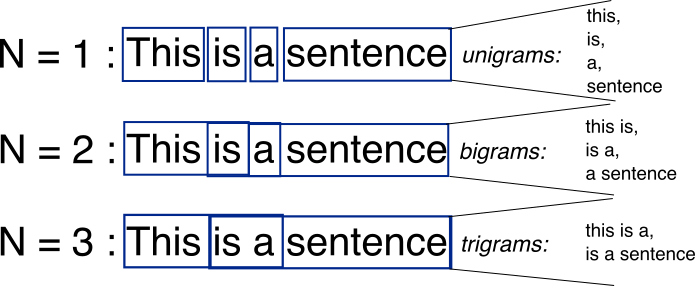
\includegraphics[width=0.6\textwidth]{../figuras/ngrams.png}
\end{figure}

O objetivo, nesse caso, é estimar a função de probabilidade $P(W_t | W_{t-(n-1)}, \cdots, W_{t-1})$, onde $W_t$ é a palavra atual e $W_{t-(n-1)}, \cdots, W_{t-1}$ representa o histórico de palavras. Sob a perspectiva estocástica, a classificação da história anterior ($W_{t-(n-1)}, \cdots, W_{t-1}$) é essencial para predizer as novas ocorrências, já que, com uma quantia suficientemente grande de textos, é possível estimar quais palavras tendem a aparecer em sequência.

No entanto, lidar com cada história textual separadamente é impraticável, já que é possível receber como entrada textos totalmente novos, sem construções de referência. A teoria de Markov, assim, surge como uma solução plausível, considerando que apenas o contexto local anterior, representado pelo conjunto das últimas palavras ($W_{t-(n-1)}, ..., W_{t-1}$), influencia a escolha da próxima ocorrência. Essa suposição leva em conta que a ordem de palavras em um texto é relevante e que geralmente existe maior correlação estatística entre unidades vizinhas, conforme pontuado em \cite{bengio-et-al-2003}.

Agrupando todas as histórias que compartilham as mesmas $n - 1$ palavras em uma mesma classe de equivalência, cria-se um modelo de Markov de ordem $n - 1$, conhecido como modelo de linguagem $N$-grama (\cite{manning-schuetze-1999}). Ao nomear tais modelos, a terminologia comumente utilizada refere-se a valores específicos de $n$, como bigrama para $n=2$ e trigrama para $n=3$. A abordagem de agrupar contextos semelhantes com base na teoria de Markov oferece uma maneira eficaz de prever palavras subsequentes em textos, com ampla aplicação no processamento de linguagem natural e análise de sentimentos.

\subsection{\textit{One-Hot Encodings}}

A técnica de \textit{one-hot encoding} é uma abordagem de representação palavras ou \textit{tokens} no âmbito do NLP. Nesse mecanismo, cada elemento do vocabulário é mapeado para um vetor binário distinto, onde todos os valores são zero, exceto aquele correspondente à posição da palavra de interesse, para a qual atribui-se o valor 1. Esse método cria representações vetoriais esparsas, cuja dimensionalidade é equivalente ao tamanho do vocabulário.

A principal característica do \textit{one-hot encoding} é a independência entre as representações de palavras. Cada uma delas é tratada como uma entidade única, sem consideração pela semelhança semântica ou relações contextuais com outras unidades do vocabulário. A representação binária resultante destaca a presença ou ausência de palavras específicas, mas não incorpora informações sobre o significado relativo delas ou suas interações semânticas.

Quando usado para codificar características ou classes, o \textit{one-hot encoding} pode ser considerado mais interpretável, dada sua natureza de independência explícita. A representação binária atribui um valor de 1 à categoria de interesse, com sua devida especificação, e 0 para todas as outras categorias, individualizando a presença ou ausência de uma característica e aumentando a interpretação de modelos, como mostrado por \citet{manai2023impact}.

Apesar de sua simplicidade e interpretabilidade, o \textit{one-hot encoding} apresenta desvantagens significativas em termos de eficiência computacional e capacidade de generalização. A representação esparsa resulta em um alto consumo de memória, especialmente em vocabulários extensos, e a falta de captura de relações semânticas limita sua utilidade em tarefas mais complexas de NLP.

\subsection{\textit{Word Embeddings}}

\textit{Word embeddings} referem-se a representações vetoriais de palavras que capturam relações semânticas e contextuais. Distintas dos $N$-gramas, que se restringem a contextos locais, essas representações incorporam informações abrangentes de todo o texto.

A origem dessas codificações remonta aos estágios iniciais dos modelos neurais probabilísticos de linguagem. Inspirados nas redes neurais de compressão de texto propostas por \citet{schmidhuber-heil-1996}, \citet{bengio-et-al-2003} conceberam um modelo de predição de palavras com uma estrutura análoga. Nesse trabalho, uma camada de projeção foi introduzida na rede neural, desempenhando o papel de mapear palavras para vetores de baixa dimensão.

Essa abordagem serviu como fundamento para o desenvolvimento de técnicas mais refinadas de \textit{word embedding}, que se disseminaram amplamente em aplicações de NLP. A representação matemática de palavras, expressa como vetores, proporciona não apenas manipulações computacionais eficientes, mas também a modelagem de aspectos semânticos pertinentes aos textos.

Lidar com representações vetoriais reais de palavras viabiliza a compreensão e exploração de relações semânticas complexas. Tais codificações permitem expressar analogias e operações sobre os elementos, como no exemplo da soma das palavras ``rei'' e ``mulher'', que resulta em vetores próximos da representação de ``rainha'' (\cite{mikolov-etal-2013-linguistic}).

\begin{figure}[ht]
    \centering
    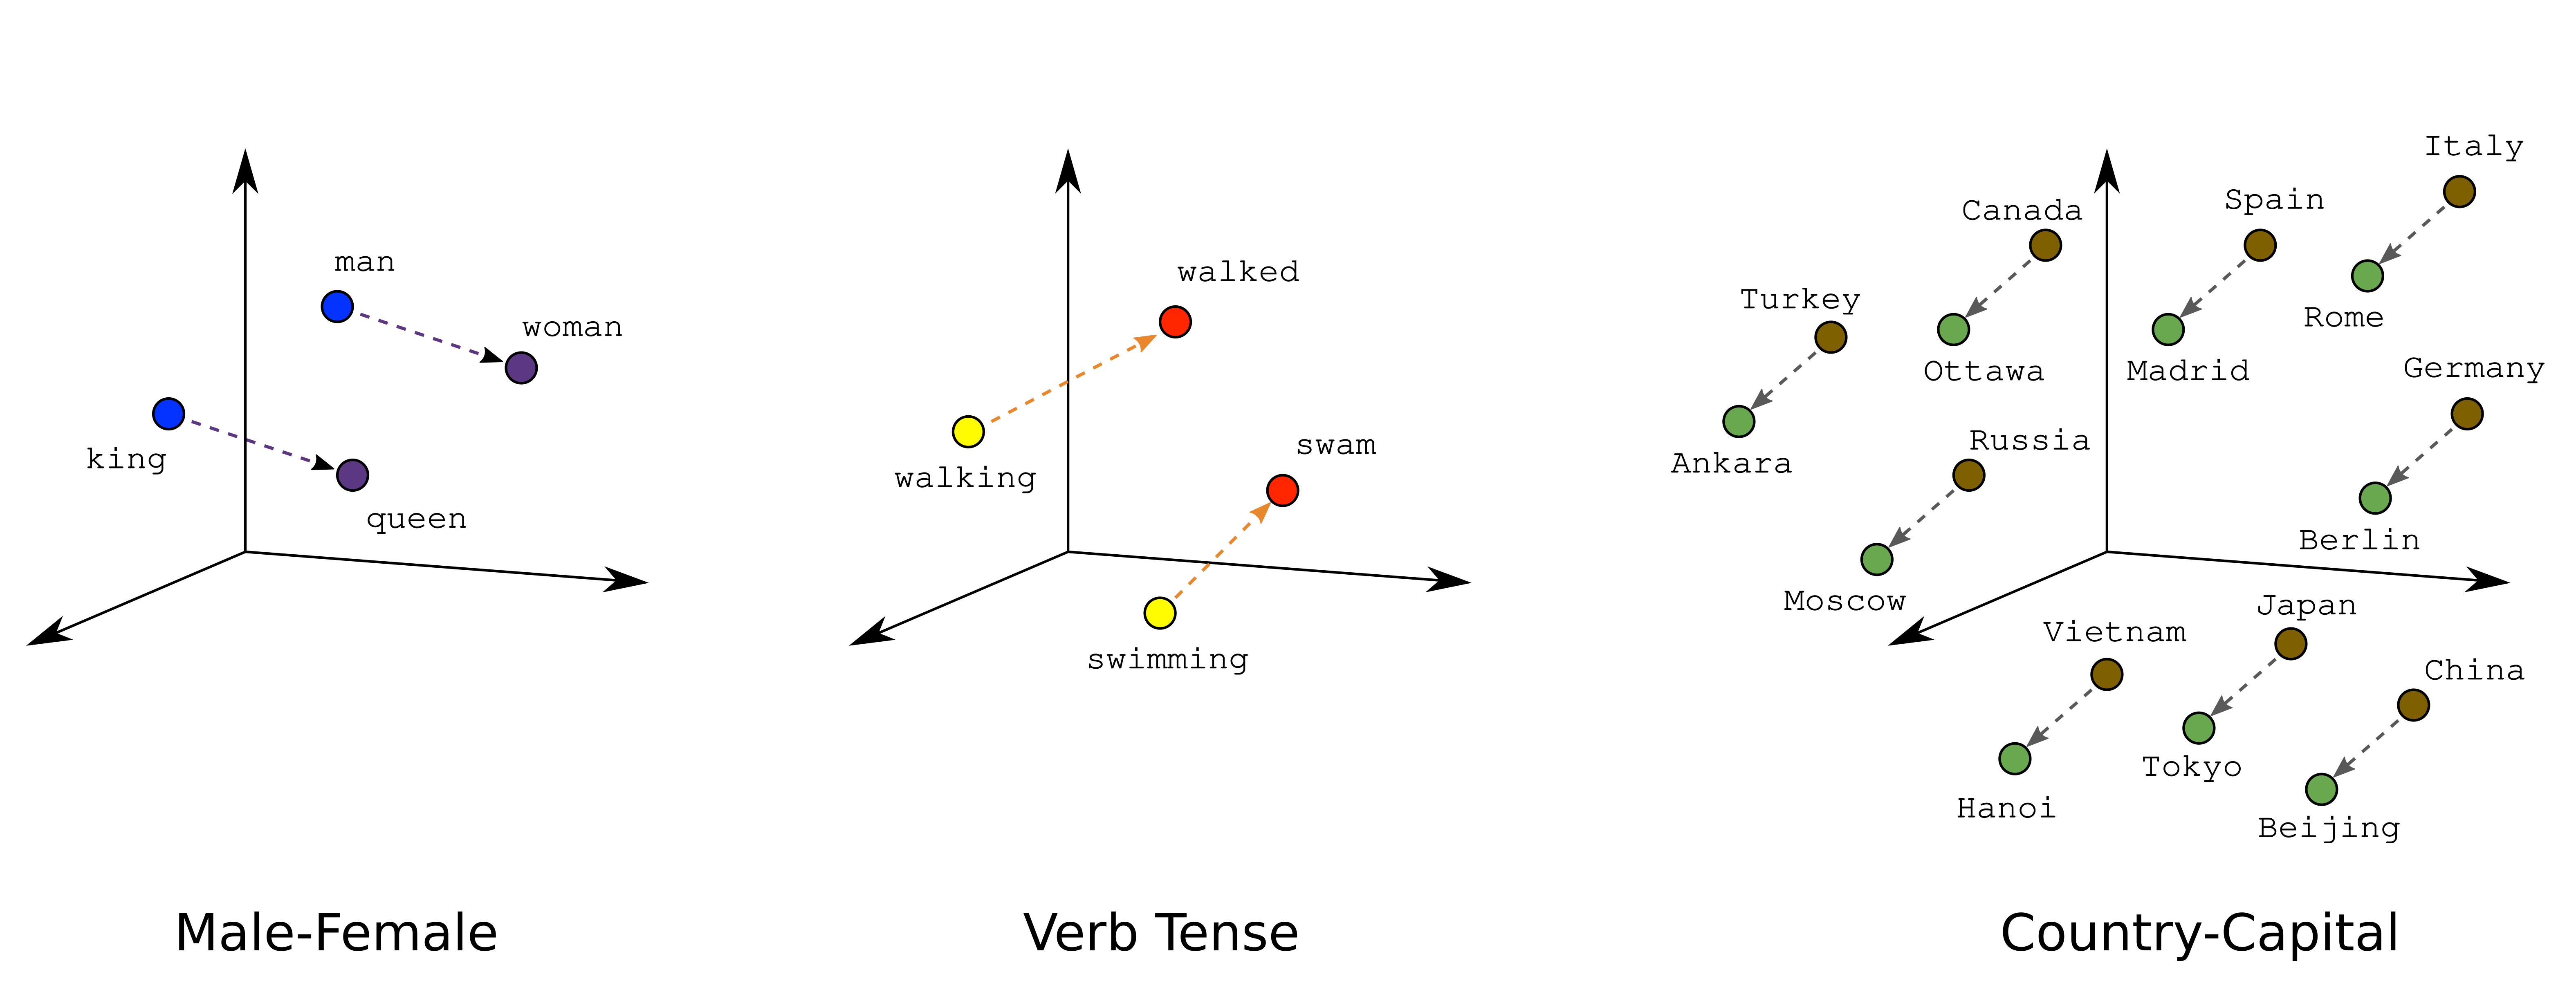
\includegraphics[width=\textwidth]{../figuras/wordembeddings.png}
    \caption{Representação vetorial de palavras sob alguns eixos semânticos. Imagem extraída de \url{https://developers.google.com/machine-learning/crash-course/embeddings/translating-to-a-lower-dimensional-space}}
    \label{fig:word_embeddings}
\end{figure}

O emprego de \textit{word embeddings} é, atualmente, mais frequente, já que o método confere vantagens significativas em termos de manipulação e compreensão semântica. Representações semelhantes a essa estrutura são empregadas em modelos de linguagem mais avançados, como o BERT. Três métodos notáveis de \textit{word embedding} são o Word2Vec, GloVe e FastText.

\subsubsection{Word2Vec}

O Word2Vec é uma técnica de \textit{word embedding} que realiza uma tradução de palavras para vetores em espaços contínuos. Este método, fundamentado em redes neurais, destaca-se por sua habilidade em preservar relações semânticas através de representações distribuídas (\cite{mikolov-etal-2013-linguistic}). O cerne do processo consiste na aprendizagem de representações que não apenas mapeiam palavras individuais, mas também capturam a proximidade semântica entre elas.

Essa codificação opera de modo a otimizar a representação vetorial de palavras com base em seu contexto geral, possibilitando a criação de \textit{embeddings} que capturam a semelhança lexical e aspectos relacionados ao significado. O modelo se destaca principalmente na incorporação de analogias e de consequências lógicas, tais quais ``\textbf{falar} está para \textbf{falado} como \textbf{escrever} está para \textbf{escrito}''.

\subsubsection{GloVe}

O GloVe (\textit{Global Vectors for Word Representation}) apresenta uma perspectiva distinta no panorama dos \textit{word embeddings}. Ele se destaca na geração de representações vetoriais fundamentadas em estatísticas globais de coocorrência de palavras em um \textit{corpus}. Essa abordagem permite uma visão abrangente das relações semânticas que transcendem contextos imediatos.

A metodologia do GloVe se baseia na construção de uma matriz de coocorrência, refletindo a probabilidade de duas palavras aparecerem juntas em um dado contexto (\cite{pennington-etal-2014-glove}). Por meio de técnicas algébricas, o modelo é usado para derivar \textit{embeddings} que melhor representem as relações semânticas capturadas por essa matriz. Dessa forma, transcende-se a limitação de representar palavras isoladamente, proporcionando uma visão holística das conexões semânticas de um texto.

\subsubsection{FastText}

O FastText, uma extensão evolutiva do Word2Vec, é um tipo de codificação que atua em nível de subpalavras. Cada palavra, nesse método, é representada por $n$-gramas de suas composições. Essa inovação confere à técnica uma notável flexibilidade na manipulação de palavras desconhecidas, capturando informações semânticas em camadas mais inferiores de um texto, e permite uma maior agilidade no processo de treinamento.

Considerar subpalavras no processo de geração de \textit{embeddings} capacita o FastText a representar os vocábulos como combinações de suas partes constituintes. Para a palavra \textit{where}, por exemplo, esse modelo pode considerar os trigramas \texttt{<wh, whe, her, ere, re>}, conforme delineado por \citet{bojanowski-etal-2016-enriching}. Isso se revela particularmente valioso em línguas com estrutura morfológica complexa, como a língua portuguesa, onde as palavras são formadas por múltiplos elementos significativos. Alguns vocábulos não conhecidos, nesse caso, podem ser construídos pelos $n$-gramas, dando poder de generalização ao modelo.

Além disso, o FastText possui uma eficácia singular no processo de treinamento, permitindo a criação de \textit{embeddings} em ambientes computacionais mais simples. Conforme evidenciado por \citet{joulin-etal-2016-bag}, métodos baseados em convoluções, tais quais os utilizados para treinar representações de Word2Vec, demonstram ser muito mais lentos que o FastText, que alcança tempos de treinamento da ordem de minutos em CPUs padrões de 20 \textit{threads}. Essa notável agilidade contribui significativamente para a adoção do FastText em tarefas de NLP que exijam rápidas codificações.

%\section{Modelos de Linguagem}

%\subsection{Modelos Baseados em N-gramas}

%\subsection{Redes Neurais Recorrentes}

%\subsection{Long Short-Term Memory}

%\subsection{Gated Recurrent Unit}

%\section{Modelos de Linguagem Baseados em Transformadores}

%\subsection{Arquitetura}

%\subsection{Mecanismo de Atenção}

%\section{BERT: Bidirectional Encoder Representations from Transformers}

%\subsection{Arquitetura}

%\subsection{Pré-treinamento}

%\subsection{Fine-tuning}

%\subsection{BERTimbau: BERT para o Português Brasileiro}

%\subsection{O BERT na Avaliação Automática de Redações}

\chapter{Metodologia}
\label{chap:work}

Com a fundamentação teórica fornecida na seção \ref{chap:fund}, exploramos as potencialidades do aprendizado profundo e do processamento de linguagem natural para desenvolver um modelo especializado na avaliação automática de redações, seguindo o formato do ENEM.

A base de dados Essay-BR, disponível em suas versões simples (\cite{marinho-et-al-21}) e estendida (\cite{marinho-et-al-22}), desempenhou um papel crucial no treinamento dos modelos avaliadores. Cada modelo foi treinado para atribuir notas a competências específicas do exame, oferecendo uma abordagem granular e detalhada para a avaliação automatizada de redações.

A arquitetura de cada sistema de avaliação foi concebida com base no processo de \textit{fine-tuning} do BERT. A estrutura envolve uma camada de entrada para a codificação dos textos e uma camada de redes neurais especializadas na atribuição de notas. O modelo escolhido para o refinamento foi o BERTimbau, pré-treinado em uma ampla gama de textos em língua portuguesa, com o objetivo principal de capturar nuances linguísticas específicas --- essenciais para a correta avaliação de redações no contexto do ENEM.

Após a fase de treinamento, submetemos cada modelo a uma avaliação rigorosa, empregando métricas de desempenho padrão, como proporção de correspondência exata e perda, além de métricas específicas do ENEM, como a avaliação consistente entre competências. Este processo visa assegurar não só a precisão geral dos sistemas avaliadores, mas também a coerência e alinhamento com os critérios estabelecidos pelo exame.

\section{Bases de dados}

Para treinar modelos de avaliação automática, partimos de uma abordagem de aprendizado supervisionado, utilizando conjuntos de redações já avaliadas por especialistas humanos. A base de dados que orientou a elaboração desse trabalho foi a Essay-BR, uma coletânea de textos no modelo do ENEM com avaliações que seguem a a matriz de referência do exame (\cite{marinho-et-al-21}; \cite{marinho-et-al-22}). % add-custom-info

As redações foram extraídas de dois portais educacionais abertos do Brasil, \href{https://vestibular.brasilescola.uol.com.br/banco-de-redacoes}{Vestibular UOL}\footnote{\url{https://vestibular.brasilescola.uol.com.br}} e \href{https://educacao.uol.com.br/bancoderedacoes}{Educação UOL}\footnote{\url{https://educacao.uol.com.br/bancoderedacoes}}, que disponibilizam a correção dos textos por especialistas da área publicamente. Em ambos os \textit{websites}, existem diferentes propostas de temas semelhantes às do ENEM, de modo que alunos podem submeter suas escritas para a avaliação de acordo com sua preferência.

Para popular a base, os autores da Essay-BR utilizaram um \textit{web crawler}, sistema encarregado de raspar de dados de sites, que coletou o conteúdo das páginas de avaliação individual em diferentes eixos temáticos. Os resultados obtidos, então, foram filtrados, com o intuito de extrair o texto e outras informações relevantes das redações, como as avaliações por competências e a pontuação geral.

Neste trabalho, visando lidar com a base de textos, utilizamos a biblioteca Pandas\footnote{\url{https://pandas.pydata.org}}, que fornece estruturas e ferramentas de análise de dados de alto desempenho, e a biblioteca Matplotlib\footnote{\url{https://matplotlib.org}}, que permite a visualização das informações em diferentes formatos de gráficos. A Essay-BR possui duas variantes de tamanho, as quais detalharemos nas seções \ref{subsec:essay-br-basic} e \ref{subsec:essay-br-extended} a seguir.

\subsection{Essay-BR Básica}
\label{subsec:essay-br-basic}

A primeira versão da Essay-BR, a que vamos referenciar como básica, contém uma quantidade de 4570 textos coletados de dezembro de 2015 a abril de 2020, contemplando uma variedade de 86 temas distintos. Desse total, 798 redações foram coletadas do Educação UOL, enquanto que 3772 redações foram obtidas do Vestibular UOL, produzindo uma coletânea rica em diferentes conteúdos e estilos de escrita.

Cada instância na base de dados é caracterizada por cinco informações relacionadas às redações: o identificador do tema (\texttt{prompt}), o título (\texttt{title}), o texto propriamente dito (\texttt{essay}), as notas atribuídas às competências (\texttt{competence}), e a pontuação final (\texttt{score}). O título, por ser opcional, pode ser vazio. Além disso, a redação é representada como uma lista de parágrafos isolados.

A avaliação das redações é expressa por meio de notas atribuídas a diferentes competências (\texttt{competence}), representadas por uma lista de 5 números inteiros que variam de 0 a 200, com incrementos de 40. Tais notas, essenciais para uma correção multifacetada, são as responsáveis por formar a pontuação final (\texttt{score}). Embora o valor de \texttt{score} seja, em essência, uma informação redundante, já que pode ser derivado da soma das notas de cada competência, sua inclusão na base de dados revela-se valiosa para a análise exploratória dos dados.

A Figura \ref{fig:essay-br-basic-analysis} ilustra, de forma visual, a distribuição das pontuações finais e das notas individuais das competências na Essay-BR básica. Essa representação gráfica revela padrões iniciais sobre a variabilidade e a dispersão dos resultados obtidos pelos alunos, proporcionando uma visão panorâmica das características gerais de avaliação.

\begin{figure}[H]
    \caption{Gráficos com a distribuição da pontuação final (à esquerda) e a distribuição das notas das competências (à direita) da Essay-BR básica.}
    \label{fig:essay-br-basic-analysis}
    \centering
    \resizebox{\textwidth}{!}{%% Creator: Matplotlib, PGF backend
%%
%% To include the figure in your LaTeX document, write
%%   \input{<filename>.pgf}
%%
%% Make sure the required packages are loaded in your preamble
%%   \usepackage{pgf}
%%
%% Also ensure that all the required font packages are loaded; for instance,
%% the lmodern package is sometimes necessary when using math font.
%%   \usepackage{lmodern}
%%
%% Figures using additional raster images can only be included by \input if
%% they are in the same directory as the main LaTeX file. For loading figures
%% from other directories you can use the `import` package
%%   \usepackage{import}
%%
%% and then include the figures with
%%   \import{<path to file>}{<filename>.pgf}
%%
%% Matplotlib used the following preamble
%%   \def\mathdefault#1{#1}
%%   \everymath=\expandafter{\the\everymath\displaystyle}
%%
%%   \usepackage{fontspec}
%%   \setmainfont{DejaVuSerif.ttf}[Path=\detokenize{/Users/josemayer/Documents/Pacotes/mambaforge/lib/python3.10/site-packages/matplotlib/mpl-data/fonts/ttf/}]
%%   \setsansfont{DejaVuSans.ttf}[Path=\detokenize{/Users/josemayer/Documents/Pacotes/mambaforge/lib/python3.10/site-packages/matplotlib/mpl-data/fonts/ttf/}]
%%   \setmonofont{DejaVuSansMono.ttf}[Path=\detokenize{/Users/josemayer/Documents/Pacotes/mambaforge/lib/python3.10/site-packages/matplotlib/mpl-data/fonts/ttf/}]
%%   \makeatletter\@ifpackageloaded{underscore}{}{\usepackage[strings]{underscore}}\makeatother
%%
\begingroup%
\makeatletter%
\begin{pgfpicture}%
\pgfpathrectangle{\pgfpointorigin}{\pgfqpoint{12.000000in}{6.000000in}}%
\pgfusepath{use as bounding box, clip}%
\begin{pgfscope}%
\pgfsetbuttcap%
\pgfsetmiterjoin%
\definecolor{currentfill}{rgb}{1.000000,1.000000,1.000000}%
\pgfsetfillcolor{currentfill}%
\pgfsetlinewidth{0.000000pt}%
\definecolor{currentstroke}{rgb}{1.000000,1.000000,1.000000}%
\pgfsetstrokecolor{currentstroke}%
\pgfsetdash{}{0pt}%
\pgfpathmoveto{\pgfqpoint{0.000000in}{0.000000in}}%
\pgfpathlineto{\pgfqpoint{12.000000in}{0.000000in}}%
\pgfpathlineto{\pgfqpoint{12.000000in}{6.000000in}}%
\pgfpathlineto{\pgfqpoint{0.000000in}{6.000000in}}%
\pgfpathlineto{\pgfqpoint{0.000000in}{0.000000in}}%
\pgfpathclose%
\pgfusepath{fill}%
\end{pgfscope}%
\begin{pgfscope}%
\pgfsetbuttcap%
\pgfsetmiterjoin%
\definecolor{currentfill}{rgb}{1.000000,1.000000,1.000000}%
\pgfsetfillcolor{currentfill}%
\pgfsetlinewidth{0.000000pt}%
\definecolor{currentstroke}{rgb}{0.000000,0.000000,0.000000}%
\pgfsetstrokecolor{currentstroke}%
\pgfsetstrokeopacity{0.000000}%
\pgfsetdash{}{0pt}%
\pgfpathmoveto{\pgfqpoint{0.709028in}{0.387222in}}%
\pgfpathlineto{\pgfqpoint{5.978715in}{0.387222in}}%
\pgfpathlineto{\pgfqpoint{5.978715in}{5.631667in}}%
\pgfpathlineto{\pgfqpoint{0.709028in}{5.631667in}}%
\pgfpathlineto{\pgfqpoint{0.709028in}{0.387222in}}%
\pgfpathclose%
\pgfusepath{fill}%
\end{pgfscope}%
\begin{pgfscope}%
\pgfpathrectangle{\pgfqpoint{0.709028in}{0.387222in}}{\pgfqpoint{5.269687in}{5.244444in}}%
\pgfusepath{clip}%
\pgfsetbuttcap%
\pgfsetmiterjoin%
\definecolor{currentfill}{rgb}{0.121569,0.466667,0.705882}%
\pgfsetfillcolor{currentfill}%
\pgfsetfillopacity{0.500000}%
\pgfsetlinewidth{1.003750pt}%
\definecolor{currentstroke}{rgb}{0.000000,0.000000,0.000000}%
\pgfsetstrokecolor{currentstroke}%
\pgfsetdash{}{0pt}%
\pgfpathmoveto{\pgfqpoint{0.948559in}{0.387222in}}%
\pgfpathlineto{\pgfqpoint{1.132814in}{0.387222in}}%
\pgfpathlineto{\pgfqpoint{1.132814in}{1.076728in}}%
\pgfpathlineto{\pgfqpoint{0.948559in}{1.076728in}}%
\pgfpathlineto{\pgfqpoint{0.948559in}{0.387222in}}%
\pgfpathclose%
\pgfusepath{stroke,fill}%
\end{pgfscope}%
\begin{pgfscope}%
\pgfpathrectangle{\pgfqpoint{0.709028in}{0.387222in}}{\pgfqpoint{5.269687in}{5.244444in}}%
\pgfusepath{clip}%
\pgfsetbuttcap%
\pgfsetmiterjoin%
\definecolor{currentfill}{rgb}{0.121569,0.466667,0.705882}%
\pgfsetfillcolor{currentfill}%
\pgfsetfillopacity{0.500000}%
\pgfsetlinewidth{1.003750pt}%
\definecolor{currentstroke}{rgb}{0.000000,0.000000,0.000000}%
\pgfsetstrokecolor{currentstroke}%
\pgfsetdash{}{0pt}%
\pgfpathmoveto{\pgfqpoint{1.132814in}{0.387222in}}%
\pgfpathlineto{\pgfqpoint{1.317069in}{0.387222in}}%
\pgfpathlineto{\pgfqpoint{1.317069in}{0.395631in}}%
\pgfpathlineto{\pgfqpoint{1.132814in}{0.395631in}}%
\pgfpathlineto{\pgfqpoint{1.132814in}{0.387222in}}%
\pgfpathclose%
\pgfusepath{stroke,fill}%
\end{pgfscope}%
\begin{pgfscope}%
\pgfpathrectangle{\pgfqpoint{0.709028in}{0.387222in}}{\pgfqpoint{5.269687in}{5.244444in}}%
\pgfusepath{clip}%
\pgfsetbuttcap%
\pgfsetmiterjoin%
\definecolor{currentfill}{rgb}{0.121569,0.466667,0.705882}%
\pgfsetfillcolor{currentfill}%
\pgfsetfillopacity{0.500000}%
\pgfsetlinewidth{1.003750pt}%
\definecolor{currentstroke}{rgb}{0.000000,0.000000,0.000000}%
\pgfsetstrokecolor{currentstroke}%
\pgfsetdash{}{0pt}%
\pgfpathmoveto{\pgfqpoint{1.317069in}{0.387222in}}%
\pgfpathlineto{\pgfqpoint{1.501323in}{0.387222in}}%
\pgfpathlineto{\pgfqpoint{1.501323in}{0.437674in}}%
\pgfpathlineto{\pgfqpoint{1.317069in}{0.437674in}}%
\pgfpathlineto{\pgfqpoint{1.317069in}{0.387222in}}%
\pgfpathclose%
\pgfusepath{stroke,fill}%
\end{pgfscope}%
\begin{pgfscope}%
\pgfpathrectangle{\pgfqpoint{0.709028in}{0.387222in}}{\pgfqpoint{5.269687in}{5.244444in}}%
\pgfusepath{clip}%
\pgfsetbuttcap%
\pgfsetmiterjoin%
\definecolor{currentfill}{rgb}{0.121569,0.466667,0.705882}%
\pgfsetfillcolor{currentfill}%
\pgfsetfillopacity{0.500000}%
\pgfsetlinewidth{1.003750pt}%
\definecolor{currentstroke}{rgb}{0.000000,0.000000,0.000000}%
\pgfsetstrokecolor{currentstroke}%
\pgfsetdash{}{0pt}%
\pgfpathmoveto{\pgfqpoint{1.501323in}{0.387222in}}%
\pgfpathlineto{\pgfqpoint{1.685578in}{0.387222in}}%
\pgfpathlineto{\pgfqpoint{1.685578in}{0.437674in}}%
\pgfpathlineto{\pgfqpoint{1.501323in}{0.437674in}}%
\pgfpathlineto{\pgfqpoint{1.501323in}{0.387222in}}%
\pgfpathclose%
\pgfusepath{stroke,fill}%
\end{pgfscope}%
\begin{pgfscope}%
\pgfpathrectangle{\pgfqpoint{0.709028in}{0.387222in}}{\pgfqpoint{5.269687in}{5.244444in}}%
\pgfusepath{clip}%
\pgfsetbuttcap%
\pgfsetmiterjoin%
\definecolor{currentfill}{rgb}{0.121569,0.466667,0.705882}%
\pgfsetfillcolor{currentfill}%
\pgfsetfillopacity{0.500000}%
\pgfsetlinewidth{1.003750pt}%
\definecolor{currentstroke}{rgb}{0.000000,0.000000,0.000000}%
\pgfsetstrokecolor{currentstroke}%
\pgfsetdash{}{0pt}%
\pgfpathmoveto{\pgfqpoint{1.685578in}{0.387222in}}%
\pgfpathlineto{\pgfqpoint{1.869833in}{0.387222in}}%
\pgfpathlineto{\pgfqpoint{1.869833in}{0.546986in}}%
\pgfpathlineto{\pgfqpoint{1.685578in}{0.546986in}}%
\pgfpathlineto{\pgfqpoint{1.685578in}{0.387222in}}%
\pgfpathclose%
\pgfusepath{stroke,fill}%
\end{pgfscope}%
\begin{pgfscope}%
\pgfpathrectangle{\pgfqpoint{0.709028in}{0.387222in}}{\pgfqpoint{5.269687in}{5.244444in}}%
\pgfusepath{clip}%
\pgfsetbuttcap%
\pgfsetmiterjoin%
\definecolor{currentfill}{rgb}{0.121569,0.466667,0.705882}%
\pgfsetfillcolor{currentfill}%
\pgfsetfillopacity{0.500000}%
\pgfsetlinewidth{1.003750pt}%
\definecolor{currentstroke}{rgb}{0.000000,0.000000,0.000000}%
\pgfsetstrokecolor{currentstroke}%
\pgfsetdash{}{0pt}%
\pgfpathmoveto{\pgfqpoint{1.869833in}{0.387222in}}%
\pgfpathlineto{\pgfqpoint{2.054088in}{0.387222in}}%
\pgfpathlineto{\pgfqpoint{2.054088in}{0.563803in}}%
\pgfpathlineto{\pgfqpoint{1.869833in}{0.563803in}}%
\pgfpathlineto{\pgfqpoint{1.869833in}{0.387222in}}%
\pgfpathclose%
\pgfusepath{stroke,fill}%
\end{pgfscope}%
\begin{pgfscope}%
\pgfpathrectangle{\pgfqpoint{0.709028in}{0.387222in}}{\pgfqpoint{5.269687in}{5.244444in}}%
\pgfusepath{clip}%
\pgfsetbuttcap%
\pgfsetmiterjoin%
\definecolor{currentfill}{rgb}{0.121569,0.466667,0.705882}%
\pgfsetfillcolor{currentfill}%
\pgfsetfillopacity{0.500000}%
\pgfsetlinewidth{1.003750pt}%
\definecolor{currentstroke}{rgb}{0.000000,0.000000,0.000000}%
\pgfsetstrokecolor{currentstroke}%
\pgfsetdash{}{0pt}%
\pgfpathmoveto{\pgfqpoint{2.054088in}{0.387222in}}%
\pgfpathlineto{\pgfqpoint{2.238343in}{0.387222in}}%
\pgfpathlineto{\pgfqpoint{2.238343in}{0.664706in}}%
\pgfpathlineto{\pgfqpoint{2.054088in}{0.664706in}}%
\pgfpathlineto{\pgfqpoint{2.054088in}{0.387222in}}%
\pgfpathclose%
\pgfusepath{stroke,fill}%
\end{pgfscope}%
\begin{pgfscope}%
\pgfpathrectangle{\pgfqpoint{0.709028in}{0.387222in}}{\pgfqpoint{5.269687in}{5.244444in}}%
\pgfusepath{clip}%
\pgfsetbuttcap%
\pgfsetmiterjoin%
\definecolor{currentfill}{rgb}{0.121569,0.466667,0.705882}%
\pgfsetfillcolor{currentfill}%
\pgfsetfillopacity{0.500000}%
\pgfsetlinewidth{1.003750pt}%
\definecolor{currentstroke}{rgb}{0.000000,0.000000,0.000000}%
\pgfsetstrokecolor{currentstroke}%
\pgfsetdash{}{0pt}%
\pgfpathmoveto{\pgfqpoint{2.238343in}{0.387222in}}%
\pgfpathlineto{\pgfqpoint{2.422597in}{0.387222in}}%
\pgfpathlineto{\pgfqpoint{2.422597in}{0.622663in}}%
\pgfpathlineto{\pgfqpoint{2.238343in}{0.622663in}}%
\pgfpathlineto{\pgfqpoint{2.238343in}{0.387222in}}%
\pgfpathclose%
\pgfusepath{stroke,fill}%
\end{pgfscope}%
\begin{pgfscope}%
\pgfpathrectangle{\pgfqpoint{0.709028in}{0.387222in}}{\pgfqpoint{5.269687in}{5.244444in}}%
\pgfusepath{clip}%
\pgfsetbuttcap%
\pgfsetmiterjoin%
\definecolor{currentfill}{rgb}{0.121569,0.466667,0.705882}%
\pgfsetfillcolor{currentfill}%
\pgfsetfillopacity{0.500000}%
\pgfsetlinewidth{1.003750pt}%
\definecolor{currentstroke}{rgb}{0.000000,0.000000,0.000000}%
\pgfsetstrokecolor{currentstroke}%
\pgfsetdash{}{0pt}%
\pgfpathmoveto{\pgfqpoint{2.422597in}{0.387222in}}%
\pgfpathlineto{\pgfqpoint{2.606852in}{0.387222in}}%
\pgfpathlineto{\pgfqpoint{2.606852in}{0.807652in}}%
\pgfpathlineto{\pgfqpoint{2.422597in}{0.807652in}}%
\pgfpathlineto{\pgfqpoint{2.422597in}{0.387222in}}%
\pgfpathclose%
\pgfusepath{stroke,fill}%
\end{pgfscope}%
\begin{pgfscope}%
\pgfpathrectangle{\pgfqpoint{0.709028in}{0.387222in}}{\pgfqpoint{5.269687in}{5.244444in}}%
\pgfusepath{clip}%
\pgfsetbuttcap%
\pgfsetmiterjoin%
\definecolor{currentfill}{rgb}{0.121569,0.466667,0.705882}%
\pgfsetfillcolor{currentfill}%
\pgfsetfillopacity{0.500000}%
\pgfsetlinewidth{1.003750pt}%
\definecolor{currentstroke}{rgb}{0.000000,0.000000,0.000000}%
\pgfsetstrokecolor{currentstroke}%
\pgfsetdash{}{0pt}%
\pgfpathmoveto{\pgfqpoint{2.606852in}{0.387222in}}%
\pgfpathlineto{\pgfqpoint{2.791107in}{0.387222in}}%
\pgfpathlineto{\pgfqpoint{2.791107in}{0.916964in}}%
\pgfpathlineto{\pgfqpoint{2.606852in}{0.916964in}}%
\pgfpathlineto{\pgfqpoint{2.606852in}{0.387222in}}%
\pgfpathclose%
\pgfusepath{stroke,fill}%
\end{pgfscope}%
\begin{pgfscope}%
\pgfpathrectangle{\pgfqpoint{0.709028in}{0.387222in}}{\pgfqpoint{5.269687in}{5.244444in}}%
\pgfusepath{clip}%
\pgfsetbuttcap%
\pgfsetmiterjoin%
\definecolor{currentfill}{rgb}{0.121569,0.466667,0.705882}%
\pgfsetfillcolor{currentfill}%
\pgfsetfillopacity{0.500000}%
\pgfsetlinewidth{1.003750pt}%
\definecolor{currentstroke}{rgb}{0.000000,0.000000,0.000000}%
\pgfsetstrokecolor{currentstroke}%
\pgfsetdash{}{0pt}%
\pgfpathmoveto{\pgfqpoint{2.791107in}{0.387222in}}%
\pgfpathlineto{\pgfqpoint{2.975362in}{0.387222in}}%
\pgfpathlineto{\pgfqpoint{2.975362in}{2.110985in}}%
\pgfpathlineto{\pgfqpoint{2.791107in}{2.110985in}}%
\pgfpathlineto{\pgfqpoint{2.791107in}{0.387222in}}%
\pgfpathclose%
\pgfusepath{stroke,fill}%
\end{pgfscope}%
\begin{pgfscope}%
\pgfpathrectangle{\pgfqpoint{0.709028in}{0.387222in}}{\pgfqpoint{5.269687in}{5.244444in}}%
\pgfusepath{clip}%
\pgfsetbuttcap%
\pgfsetmiterjoin%
\definecolor{currentfill}{rgb}{0.121569,0.466667,0.705882}%
\pgfsetfillcolor{currentfill}%
\pgfsetfillopacity{0.500000}%
\pgfsetlinewidth{1.003750pt}%
\definecolor{currentstroke}{rgb}{0.000000,0.000000,0.000000}%
\pgfsetstrokecolor{currentstroke}%
\pgfsetdash{}{0pt}%
\pgfpathmoveto{\pgfqpoint{2.975362in}{0.387222in}}%
\pgfpathlineto{\pgfqpoint{3.159617in}{0.387222in}}%
\pgfpathlineto{\pgfqpoint{3.159617in}{2.186663in}}%
\pgfpathlineto{\pgfqpoint{2.975362in}{2.186663in}}%
\pgfpathlineto{\pgfqpoint{2.975362in}{0.387222in}}%
\pgfpathclose%
\pgfusepath{stroke,fill}%
\end{pgfscope}%
\begin{pgfscope}%
\pgfpathrectangle{\pgfqpoint{0.709028in}{0.387222in}}{\pgfqpoint{5.269687in}{5.244444in}}%
\pgfusepath{clip}%
\pgfsetbuttcap%
\pgfsetmiterjoin%
\definecolor{currentfill}{rgb}{0.121569,0.466667,0.705882}%
\pgfsetfillcolor{currentfill}%
\pgfsetfillopacity{0.500000}%
\pgfsetlinewidth{1.003750pt}%
\definecolor{currentstroke}{rgb}{0.000000,0.000000,0.000000}%
\pgfsetstrokecolor{currentstroke}%
\pgfsetdash{}{0pt}%
\pgfpathmoveto{\pgfqpoint{3.159617in}{0.387222in}}%
\pgfpathlineto{\pgfqpoint{3.343872in}{0.387222in}}%
\pgfpathlineto{\pgfqpoint{3.343872in}{2.724813in}}%
\pgfpathlineto{\pgfqpoint{3.159617in}{2.724813in}}%
\pgfpathlineto{\pgfqpoint{3.159617in}{0.387222in}}%
\pgfpathclose%
\pgfusepath{stroke,fill}%
\end{pgfscope}%
\begin{pgfscope}%
\pgfpathrectangle{\pgfqpoint{0.709028in}{0.387222in}}{\pgfqpoint{5.269687in}{5.244444in}}%
\pgfusepath{clip}%
\pgfsetbuttcap%
\pgfsetmiterjoin%
\definecolor{currentfill}{rgb}{0.121569,0.466667,0.705882}%
\pgfsetfillcolor{currentfill}%
\pgfsetfillopacity{0.500000}%
\pgfsetlinewidth{1.003750pt}%
\definecolor{currentstroke}{rgb}{0.000000,0.000000,0.000000}%
\pgfsetstrokecolor{currentstroke}%
\pgfsetdash{}{0pt}%
\pgfpathmoveto{\pgfqpoint{3.343872in}{0.387222in}}%
\pgfpathlineto{\pgfqpoint{3.528126in}{0.387222in}}%
\pgfpathlineto{\pgfqpoint{3.528126in}{3.649759in}}%
\pgfpathlineto{\pgfqpoint{3.343872in}{3.649759in}}%
\pgfpathlineto{\pgfqpoint{3.343872in}{0.387222in}}%
\pgfpathclose%
\pgfusepath{stroke,fill}%
\end{pgfscope}%
\begin{pgfscope}%
\pgfpathrectangle{\pgfqpoint{0.709028in}{0.387222in}}{\pgfqpoint{5.269687in}{5.244444in}}%
\pgfusepath{clip}%
\pgfsetbuttcap%
\pgfsetmiterjoin%
\definecolor{currentfill}{rgb}{0.121569,0.466667,0.705882}%
\pgfsetfillcolor{currentfill}%
\pgfsetfillopacity{0.500000}%
\pgfsetlinewidth{1.003750pt}%
\definecolor{currentstroke}{rgb}{0.000000,0.000000,0.000000}%
\pgfsetstrokecolor{currentstroke}%
\pgfsetdash{}{0pt}%
\pgfpathmoveto{\pgfqpoint{3.528126in}{0.387222in}}%
\pgfpathlineto{\pgfqpoint{3.712381in}{0.387222in}}%
\pgfpathlineto{\pgfqpoint{3.712381in}{3.321824in}}%
\pgfpathlineto{\pgfqpoint{3.528126in}{3.321824in}}%
\pgfpathlineto{\pgfqpoint{3.528126in}{0.387222in}}%
\pgfpathclose%
\pgfusepath{stroke,fill}%
\end{pgfscope}%
\begin{pgfscope}%
\pgfpathrectangle{\pgfqpoint{0.709028in}{0.387222in}}{\pgfqpoint{5.269687in}{5.244444in}}%
\pgfusepath{clip}%
\pgfsetbuttcap%
\pgfsetmiterjoin%
\definecolor{currentfill}{rgb}{0.121569,0.466667,0.705882}%
\pgfsetfillcolor{currentfill}%
\pgfsetfillopacity{0.500000}%
\pgfsetlinewidth{1.003750pt}%
\definecolor{currentstroke}{rgb}{0.000000,0.000000,0.000000}%
\pgfsetstrokecolor{currentstroke}%
\pgfsetdash{}{0pt}%
\pgfpathmoveto{\pgfqpoint{3.712381in}{0.387222in}}%
\pgfpathlineto{\pgfqpoint{3.896636in}{0.387222in}}%
\pgfpathlineto{\pgfqpoint{3.896636in}{5.381931in}}%
\pgfpathlineto{\pgfqpoint{3.712381in}{5.381931in}}%
\pgfpathlineto{\pgfqpoint{3.712381in}{0.387222in}}%
\pgfpathclose%
\pgfusepath{stroke,fill}%
\end{pgfscope}%
\begin{pgfscope}%
\pgfpathrectangle{\pgfqpoint{0.709028in}{0.387222in}}{\pgfqpoint{5.269687in}{5.244444in}}%
\pgfusepath{clip}%
\pgfsetbuttcap%
\pgfsetmiterjoin%
\definecolor{currentfill}{rgb}{0.121569,0.466667,0.705882}%
\pgfsetfillcolor{currentfill}%
\pgfsetfillopacity{0.500000}%
\pgfsetlinewidth{1.003750pt}%
\definecolor{currentstroke}{rgb}{0.000000,0.000000,0.000000}%
\pgfsetstrokecolor{currentstroke}%
\pgfsetdash{}{0pt}%
\pgfpathmoveto{\pgfqpoint{3.896636in}{0.387222in}}%
\pgfpathlineto{\pgfqpoint{4.080891in}{0.387222in}}%
\pgfpathlineto{\pgfqpoint{4.080891in}{2.817308in}}%
\pgfpathlineto{\pgfqpoint{3.896636in}{2.817308in}}%
\pgfpathlineto{\pgfqpoint{3.896636in}{0.387222in}}%
\pgfpathclose%
\pgfusepath{stroke,fill}%
\end{pgfscope}%
\begin{pgfscope}%
\pgfpathrectangle{\pgfqpoint{0.709028in}{0.387222in}}{\pgfqpoint{5.269687in}{5.244444in}}%
\pgfusepath{clip}%
\pgfsetbuttcap%
\pgfsetmiterjoin%
\definecolor{currentfill}{rgb}{0.121569,0.466667,0.705882}%
\pgfsetfillcolor{currentfill}%
\pgfsetfillopacity{0.500000}%
\pgfsetlinewidth{1.003750pt}%
\definecolor{currentstroke}{rgb}{0.000000,0.000000,0.000000}%
\pgfsetstrokecolor{currentstroke}%
\pgfsetdash{}{0pt}%
\pgfpathmoveto{\pgfqpoint{4.080891in}{0.387222in}}%
\pgfpathlineto{\pgfqpoint{4.265146in}{0.387222in}}%
\pgfpathlineto{\pgfqpoint{4.265146in}{4.490620in}}%
\pgfpathlineto{\pgfqpoint{4.080891in}{4.490620in}}%
\pgfpathlineto{\pgfqpoint{4.080891in}{0.387222in}}%
\pgfpathclose%
\pgfusepath{stroke,fill}%
\end{pgfscope}%
\begin{pgfscope}%
\pgfpathrectangle{\pgfqpoint{0.709028in}{0.387222in}}{\pgfqpoint{5.269687in}{5.244444in}}%
\pgfusepath{clip}%
\pgfsetbuttcap%
\pgfsetmiterjoin%
\definecolor{currentfill}{rgb}{0.121569,0.466667,0.705882}%
\pgfsetfillcolor{currentfill}%
\pgfsetfillopacity{0.500000}%
\pgfsetlinewidth{1.003750pt}%
\definecolor{currentstroke}{rgb}{0.000000,0.000000,0.000000}%
\pgfsetstrokecolor{currentstroke}%
\pgfsetdash{}{0pt}%
\pgfpathmoveto{\pgfqpoint{4.265146in}{0.387222in}}%
\pgfpathlineto{\pgfqpoint{4.449400in}{0.387222in}}%
\pgfpathlineto{\pgfqpoint{4.449400in}{3.717028in}}%
\pgfpathlineto{\pgfqpoint{4.265146in}{3.717028in}}%
\pgfpathlineto{\pgfqpoint{4.265146in}{0.387222in}}%
\pgfpathclose%
\pgfusepath{stroke,fill}%
\end{pgfscope}%
\begin{pgfscope}%
\pgfpathrectangle{\pgfqpoint{0.709028in}{0.387222in}}{\pgfqpoint{5.269687in}{5.244444in}}%
\pgfusepath{clip}%
\pgfsetbuttcap%
\pgfsetmiterjoin%
\definecolor{currentfill}{rgb}{0.121569,0.466667,0.705882}%
\pgfsetfillcolor{currentfill}%
\pgfsetfillopacity{0.500000}%
\pgfsetlinewidth{1.003750pt}%
\definecolor{currentstroke}{rgb}{0.000000,0.000000,0.000000}%
\pgfsetstrokecolor{currentstroke}%
\pgfsetdash{}{0pt}%
\pgfpathmoveto{\pgfqpoint{4.449400in}{0.387222in}}%
\pgfpathlineto{\pgfqpoint{4.633655in}{0.387222in}}%
\pgfpathlineto{\pgfqpoint{4.633655in}{2.699587in}}%
\pgfpathlineto{\pgfqpoint{4.449400in}{2.699587in}}%
\pgfpathlineto{\pgfqpoint{4.449400in}{0.387222in}}%
\pgfpathclose%
\pgfusepath{stroke,fill}%
\end{pgfscope}%
\begin{pgfscope}%
\pgfpathrectangle{\pgfqpoint{0.709028in}{0.387222in}}{\pgfqpoint{5.269687in}{5.244444in}}%
\pgfusepath{clip}%
\pgfsetbuttcap%
\pgfsetmiterjoin%
\definecolor{currentfill}{rgb}{0.121569,0.466667,0.705882}%
\pgfsetfillcolor{currentfill}%
\pgfsetfillopacity{0.500000}%
\pgfsetlinewidth{1.003750pt}%
\definecolor{currentstroke}{rgb}{0.000000,0.000000,0.000000}%
\pgfsetstrokecolor{currentstroke}%
\pgfsetdash{}{0pt}%
\pgfpathmoveto{\pgfqpoint{4.633655in}{0.387222in}}%
\pgfpathlineto{\pgfqpoint{4.817910in}{0.387222in}}%
\pgfpathlineto{\pgfqpoint{4.817910in}{2.775265in}}%
\pgfpathlineto{\pgfqpoint{4.633655in}{2.775265in}}%
\pgfpathlineto{\pgfqpoint{4.633655in}{0.387222in}}%
\pgfpathclose%
\pgfusepath{stroke,fill}%
\end{pgfscope}%
\begin{pgfscope}%
\pgfpathrectangle{\pgfqpoint{0.709028in}{0.387222in}}{\pgfqpoint{5.269687in}{5.244444in}}%
\pgfusepath{clip}%
\pgfsetbuttcap%
\pgfsetmiterjoin%
\definecolor{currentfill}{rgb}{0.121569,0.466667,0.705882}%
\pgfsetfillcolor{currentfill}%
\pgfsetfillopacity{0.500000}%
\pgfsetlinewidth{1.003750pt}%
\definecolor{currentstroke}{rgb}{0.000000,0.000000,0.000000}%
\pgfsetstrokecolor{currentstroke}%
\pgfsetdash{}{0pt}%
\pgfpathmoveto{\pgfqpoint{4.817910in}{0.387222in}}%
\pgfpathlineto{\pgfqpoint{5.002165in}{0.387222in}}%
\pgfpathlineto{\pgfqpoint{5.002165in}{2.094168in}}%
\pgfpathlineto{\pgfqpoint{4.817910in}{2.094168in}}%
\pgfpathlineto{\pgfqpoint{4.817910in}{0.387222in}}%
\pgfpathclose%
\pgfusepath{stroke,fill}%
\end{pgfscope}%
\begin{pgfscope}%
\pgfpathrectangle{\pgfqpoint{0.709028in}{0.387222in}}{\pgfqpoint{5.269687in}{5.244444in}}%
\pgfusepath{clip}%
\pgfsetbuttcap%
\pgfsetmiterjoin%
\definecolor{currentfill}{rgb}{0.121569,0.466667,0.705882}%
\pgfsetfillcolor{currentfill}%
\pgfsetfillopacity{0.500000}%
\pgfsetlinewidth{1.003750pt}%
\definecolor{currentstroke}{rgb}{0.000000,0.000000,0.000000}%
\pgfsetstrokecolor{currentstroke}%
\pgfsetdash{}{0pt}%
\pgfpathmoveto{\pgfqpoint{5.002165in}{0.387222in}}%
\pgfpathlineto{\pgfqpoint{5.186420in}{0.387222in}}%
\pgfpathlineto{\pgfqpoint{5.186420in}{1.656921in}}%
\pgfpathlineto{\pgfqpoint{5.002165in}{1.656921in}}%
\pgfpathlineto{\pgfqpoint{5.002165in}{0.387222in}}%
\pgfpathclose%
\pgfusepath{stroke,fill}%
\end{pgfscope}%
\begin{pgfscope}%
\pgfpathrectangle{\pgfqpoint{0.709028in}{0.387222in}}{\pgfqpoint{5.269687in}{5.244444in}}%
\pgfusepath{clip}%
\pgfsetbuttcap%
\pgfsetmiterjoin%
\definecolor{currentfill}{rgb}{0.121569,0.466667,0.705882}%
\pgfsetfillcolor{currentfill}%
\pgfsetfillopacity{0.500000}%
\pgfsetlinewidth{1.003750pt}%
\definecolor{currentstroke}{rgb}{0.000000,0.000000,0.000000}%
\pgfsetstrokecolor{currentstroke}%
\pgfsetdash{}{0pt}%
\pgfpathmoveto{\pgfqpoint{5.186420in}{0.387222in}}%
\pgfpathlineto{\pgfqpoint{5.370674in}{0.387222in}}%
\pgfpathlineto{\pgfqpoint{5.370674in}{1.143996in}}%
\pgfpathlineto{\pgfqpoint{5.186420in}{1.143996in}}%
\pgfpathlineto{\pgfqpoint{5.186420in}{0.387222in}}%
\pgfpathclose%
\pgfusepath{stroke,fill}%
\end{pgfscope}%
\begin{pgfscope}%
\pgfpathrectangle{\pgfqpoint{0.709028in}{0.387222in}}{\pgfqpoint{5.269687in}{5.244444in}}%
\pgfusepath{clip}%
\pgfsetbuttcap%
\pgfsetmiterjoin%
\definecolor{currentfill}{rgb}{0.121569,0.466667,0.705882}%
\pgfsetfillcolor{currentfill}%
\pgfsetfillopacity{0.500000}%
\pgfsetlinewidth{1.003750pt}%
\definecolor{currentstroke}{rgb}{0.000000,0.000000,0.000000}%
\pgfsetstrokecolor{currentstroke}%
\pgfsetdash{}{0pt}%
\pgfpathmoveto{\pgfqpoint{5.370674in}{0.387222in}}%
\pgfpathlineto{\pgfqpoint{5.554929in}{0.387222in}}%
\pgfpathlineto{\pgfqpoint{5.554929in}{0.664706in}}%
\pgfpathlineto{\pgfqpoint{5.370674in}{0.664706in}}%
\pgfpathlineto{\pgfqpoint{5.370674in}{0.387222in}}%
\pgfpathclose%
\pgfusepath{stroke,fill}%
\end{pgfscope}%
\begin{pgfscope}%
\pgfpathrectangle{\pgfqpoint{0.709028in}{0.387222in}}{\pgfqpoint{5.269687in}{5.244444in}}%
\pgfusepath{clip}%
\pgfsetbuttcap%
\pgfsetmiterjoin%
\definecolor{currentfill}{rgb}{0.121569,0.466667,0.705882}%
\pgfsetfillcolor{currentfill}%
\pgfsetfillopacity{0.500000}%
\pgfsetlinewidth{1.003750pt}%
\definecolor{currentstroke}{rgb}{0.000000,0.000000,0.000000}%
\pgfsetstrokecolor{currentstroke}%
\pgfsetdash{}{0pt}%
\pgfpathmoveto{\pgfqpoint{5.554929in}{0.387222in}}%
\pgfpathlineto{\pgfqpoint{5.739184in}{0.387222in}}%
\pgfpathlineto{\pgfqpoint{5.739184in}{0.589029in}}%
\pgfpathlineto{\pgfqpoint{5.554929in}{0.589029in}}%
\pgfpathlineto{\pgfqpoint{5.554929in}{0.387222in}}%
\pgfpathclose%
\pgfusepath{stroke,fill}%
\end{pgfscope}%
\begin{pgfscope}%
\pgfsetbuttcap%
\pgfsetroundjoin%
\definecolor{currentfill}{rgb}{0.000000,0.000000,0.000000}%
\pgfsetfillcolor{currentfill}%
\pgfsetlinewidth{0.803000pt}%
\definecolor{currentstroke}{rgb}{0.000000,0.000000,0.000000}%
\pgfsetstrokecolor{currentstroke}%
\pgfsetdash{}{0pt}%
\pgfsys@defobject{currentmarker}{\pgfqpoint{0.000000in}{-0.048611in}}{\pgfqpoint{0.000000in}{0.000000in}}{%
\pgfpathmoveto{\pgfqpoint{0.000000in}{0.000000in}}%
\pgfpathlineto{\pgfqpoint{0.000000in}{-0.048611in}}%
\pgfusepath{stroke,fill}%
}%
\begin{pgfscope}%
\pgfsys@transformshift{0.948559in}{0.387222in}%
\pgfsys@useobject{currentmarker}{}%
\end{pgfscope}%
\end{pgfscope}%
\begin{pgfscope}%
\definecolor{textcolor}{rgb}{0.000000,0.000000,0.000000}%
\pgfsetstrokecolor{textcolor}%
\pgfsetfillcolor{textcolor}%
\pgftext[x=0.948559in,y=0.290000in,,top]{\color{textcolor}{\sffamily\fontsize{10.000000}{12.000000}\selectfont\catcode`\^=\active\def^{\ifmmode\sp\else\^{}\fi}\catcode`\%=\active\def%{\%}0}}%
\end{pgfscope}%
\begin{pgfscope}%
\pgfsetbuttcap%
\pgfsetroundjoin%
\definecolor{currentfill}{rgb}{0.000000,0.000000,0.000000}%
\pgfsetfillcolor{currentfill}%
\pgfsetlinewidth{0.803000pt}%
\definecolor{currentstroke}{rgb}{0.000000,0.000000,0.000000}%
\pgfsetstrokecolor{currentstroke}%
\pgfsetdash{}{0pt}%
\pgfsys@defobject{currentmarker}{\pgfqpoint{0.000000in}{-0.048611in}}{\pgfqpoint{0.000000in}{0.000000in}}{%
\pgfpathmoveto{\pgfqpoint{0.000000in}{0.000000in}}%
\pgfpathlineto{\pgfqpoint{0.000000in}{-0.048611in}}%
\pgfusepath{stroke,fill}%
}%
\begin{pgfscope}%
\pgfsys@transformshift{1.869833in}{0.387222in}%
\pgfsys@useobject{currentmarker}{}%
\end{pgfscope}%
\end{pgfscope}%
\begin{pgfscope}%
\definecolor{textcolor}{rgb}{0.000000,0.000000,0.000000}%
\pgfsetstrokecolor{textcolor}%
\pgfsetfillcolor{textcolor}%
\pgftext[x=1.869833in,y=0.290000in,,top]{\color{textcolor}{\sffamily\fontsize{10.000000}{12.000000}\selectfont\catcode`\^=\active\def^{\ifmmode\sp\else\^{}\fi}\catcode`\%=\active\def%{\%}200}}%
\end{pgfscope}%
\begin{pgfscope}%
\pgfsetbuttcap%
\pgfsetroundjoin%
\definecolor{currentfill}{rgb}{0.000000,0.000000,0.000000}%
\pgfsetfillcolor{currentfill}%
\pgfsetlinewidth{0.803000pt}%
\definecolor{currentstroke}{rgb}{0.000000,0.000000,0.000000}%
\pgfsetstrokecolor{currentstroke}%
\pgfsetdash{}{0pt}%
\pgfsys@defobject{currentmarker}{\pgfqpoint{0.000000in}{-0.048611in}}{\pgfqpoint{0.000000in}{0.000000in}}{%
\pgfpathmoveto{\pgfqpoint{0.000000in}{0.000000in}}%
\pgfpathlineto{\pgfqpoint{0.000000in}{-0.048611in}}%
\pgfusepath{stroke,fill}%
}%
\begin{pgfscope}%
\pgfsys@transformshift{2.791107in}{0.387222in}%
\pgfsys@useobject{currentmarker}{}%
\end{pgfscope}%
\end{pgfscope}%
\begin{pgfscope}%
\definecolor{textcolor}{rgb}{0.000000,0.000000,0.000000}%
\pgfsetstrokecolor{textcolor}%
\pgfsetfillcolor{textcolor}%
\pgftext[x=2.791107in,y=0.290000in,,top]{\color{textcolor}{\sffamily\fontsize{10.000000}{12.000000}\selectfont\catcode`\^=\active\def^{\ifmmode\sp\else\^{}\fi}\catcode`\%=\active\def%{\%}400}}%
\end{pgfscope}%
\begin{pgfscope}%
\pgfsetbuttcap%
\pgfsetroundjoin%
\definecolor{currentfill}{rgb}{0.000000,0.000000,0.000000}%
\pgfsetfillcolor{currentfill}%
\pgfsetlinewidth{0.803000pt}%
\definecolor{currentstroke}{rgb}{0.000000,0.000000,0.000000}%
\pgfsetstrokecolor{currentstroke}%
\pgfsetdash{}{0pt}%
\pgfsys@defobject{currentmarker}{\pgfqpoint{0.000000in}{-0.048611in}}{\pgfqpoint{0.000000in}{0.000000in}}{%
\pgfpathmoveto{\pgfqpoint{0.000000in}{0.000000in}}%
\pgfpathlineto{\pgfqpoint{0.000000in}{-0.048611in}}%
\pgfusepath{stroke,fill}%
}%
\begin{pgfscope}%
\pgfsys@transformshift{3.712381in}{0.387222in}%
\pgfsys@useobject{currentmarker}{}%
\end{pgfscope}%
\end{pgfscope}%
\begin{pgfscope}%
\definecolor{textcolor}{rgb}{0.000000,0.000000,0.000000}%
\pgfsetstrokecolor{textcolor}%
\pgfsetfillcolor{textcolor}%
\pgftext[x=3.712381in,y=0.290000in,,top]{\color{textcolor}{\sffamily\fontsize{10.000000}{12.000000}\selectfont\catcode`\^=\active\def^{\ifmmode\sp\else\^{}\fi}\catcode`\%=\active\def%{\%}600}}%
\end{pgfscope}%
\begin{pgfscope}%
\pgfsetbuttcap%
\pgfsetroundjoin%
\definecolor{currentfill}{rgb}{0.000000,0.000000,0.000000}%
\pgfsetfillcolor{currentfill}%
\pgfsetlinewidth{0.803000pt}%
\definecolor{currentstroke}{rgb}{0.000000,0.000000,0.000000}%
\pgfsetstrokecolor{currentstroke}%
\pgfsetdash{}{0pt}%
\pgfsys@defobject{currentmarker}{\pgfqpoint{0.000000in}{-0.048611in}}{\pgfqpoint{0.000000in}{0.000000in}}{%
\pgfpathmoveto{\pgfqpoint{0.000000in}{0.000000in}}%
\pgfpathlineto{\pgfqpoint{0.000000in}{-0.048611in}}%
\pgfusepath{stroke,fill}%
}%
\begin{pgfscope}%
\pgfsys@transformshift{4.633655in}{0.387222in}%
\pgfsys@useobject{currentmarker}{}%
\end{pgfscope}%
\end{pgfscope}%
\begin{pgfscope}%
\definecolor{textcolor}{rgb}{0.000000,0.000000,0.000000}%
\pgfsetstrokecolor{textcolor}%
\pgfsetfillcolor{textcolor}%
\pgftext[x=4.633655in,y=0.290000in,,top]{\color{textcolor}{\sffamily\fontsize{10.000000}{12.000000}\selectfont\catcode`\^=\active\def^{\ifmmode\sp\else\^{}\fi}\catcode`\%=\active\def%{\%}800}}%
\end{pgfscope}%
\begin{pgfscope}%
\pgfsetbuttcap%
\pgfsetroundjoin%
\definecolor{currentfill}{rgb}{0.000000,0.000000,0.000000}%
\pgfsetfillcolor{currentfill}%
\pgfsetlinewidth{0.803000pt}%
\definecolor{currentstroke}{rgb}{0.000000,0.000000,0.000000}%
\pgfsetstrokecolor{currentstroke}%
\pgfsetdash{}{0pt}%
\pgfsys@defobject{currentmarker}{\pgfqpoint{0.000000in}{-0.048611in}}{\pgfqpoint{0.000000in}{0.000000in}}{%
\pgfpathmoveto{\pgfqpoint{0.000000in}{0.000000in}}%
\pgfpathlineto{\pgfqpoint{0.000000in}{-0.048611in}}%
\pgfusepath{stroke,fill}%
}%
\begin{pgfscope}%
\pgfsys@transformshift{5.554929in}{0.387222in}%
\pgfsys@useobject{currentmarker}{}%
\end{pgfscope}%
\end{pgfscope}%
\begin{pgfscope}%
\definecolor{textcolor}{rgb}{0.000000,0.000000,0.000000}%
\pgfsetstrokecolor{textcolor}%
\pgfsetfillcolor{textcolor}%
\pgftext[x=5.554929in,y=0.290000in,,top]{\color{textcolor}{\sffamily\fontsize{10.000000}{12.000000}\selectfont\catcode`\^=\active\def^{\ifmmode\sp\else\^{}\fi}\catcode`\%=\active\def%{\%}1000}}%
\end{pgfscope}%
\begin{pgfscope}%
\pgfsetbuttcap%
\pgfsetroundjoin%
\definecolor{currentfill}{rgb}{0.000000,0.000000,0.000000}%
\pgfsetfillcolor{currentfill}%
\pgfsetlinewidth{0.803000pt}%
\definecolor{currentstroke}{rgb}{0.000000,0.000000,0.000000}%
\pgfsetstrokecolor{currentstroke}%
\pgfsetdash{}{0pt}%
\pgfsys@defobject{currentmarker}{\pgfqpoint{-0.048611in}{0.000000in}}{\pgfqpoint{-0.000000in}{0.000000in}}{%
\pgfpathmoveto{\pgfqpoint{-0.000000in}{0.000000in}}%
\pgfpathlineto{\pgfqpoint{-0.048611in}{0.000000in}}%
\pgfusepath{stroke,fill}%
}%
\begin{pgfscope}%
\pgfsys@transformshift{0.709028in}{0.387222in}%
\pgfsys@useobject{currentmarker}{}%
\end{pgfscope}%
\end{pgfscope}%
\begin{pgfscope}%
\definecolor{textcolor}{rgb}{0.000000,0.000000,0.000000}%
\pgfsetstrokecolor{textcolor}%
\pgfsetfillcolor{textcolor}%
\pgftext[x=0.523440in, y=0.334461in, left, base]{\color{textcolor}{\sffamily\fontsize{10.000000}{12.000000}\selectfont\catcode`\^=\active\def^{\ifmmode\sp\else\^{}\fi}\catcode`\%=\active\def%{\%}0}}%
\end{pgfscope}%
\begin{pgfscope}%
\pgfsetbuttcap%
\pgfsetroundjoin%
\definecolor{currentfill}{rgb}{0.000000,0.000000,0.000000}%
\pgfsetfillcolor{currentfill}%
\pgfsetlinewidth{0.803000pt}%
\definecolor{currentstroke}{rgb}{0.000000,0.000000,0.000000}%
\pgfsetstrokecolor{currentstroke}%
\pgfsetdash{}{0pt}%
\pgfsys@defobject{currentmarker}{\pgfqpoint{-0.048611in}{0.000000in}}{\pgfqpoint{-0.000000in}{0.000000in}}{%
\pgfpathmoveto{\pgfqpoint{-0.000000in}{0.000000in}}%
\pgfpathlineto{\pgfqpoint{-0.048611in}{0.000000in}}%
\pgfusepath{stroke,fill}%
}%
\begin{pgfscope}%
\pgfsys@transformshift{0.709028in}{1.228082in}%
\pgfsys@useobject{currentmarker}{}%
\end{pgfscope}%
\end{pgfscope}%
\begin{pgfscope}%
\definecolor{textcolor}{rgb}{0.000000,0.000000,0.000000}%
\pgfsetstrokecolor{textcolor}%
\pgfsetfillcolor{textcolor}%
\pgftext[x=0.346710in, y=1.175321in, left, base]{\color{textcolor}{\sffamily\fontsize{10.000000}{12.000000}\selectfont\catcode`\^=\active\def^{\ifmmode\sp\else\^{}\fi}\catcode`\%=\active\def%{\%}100}}%
\end{pgfscope}%
\begin{pgfscope}%
\pgfsetbuttcap%
\pgfsetroundjoin%
\definecolor{currentfill}{rgb}{0.000000,0.000000,0.000000}%
\pgfsetfillcolor{currentfill}%
\pgfsetlinewidth{0.803000pt}%
\definecolor{currentstroke}{rgb}{0.000000,0.000000,0.000000}%
\pgfsetstrokecolor{currentstroke}%
\pgfsetdash{}{0pt}%
\pgfsys@defobject{currentmarker}{\pgfqpoint{-0.048611in}{0.000000in}}{\pgfqpoint{-0.000000in}{0.000000in}}{%
\pgfpathmoveto{\pgfqpoint{-0.000000in}{0.000000in}}%
\pgfpathlineto{\pgfqpoint{-0.048611in}{0.000000in}}%
\pgfusepath{stroke,fill}%
}%
\begin{pgfscope}%
\pgfsys@transformshift{0.709028in}{2.068942in}%
\pgfsys@useobject{currentmarker}{}%
\end{pgfscope}%
\end{pgfscope}%
\begin{pgfscope}%
\definecolor{textcolor}{rgb}{0.000000,0.000000,0.000000}%
\pgfsetstrokecolor{textcolor}%
\pgfsetfillcolor{textcolor}%
\pgftext[x=0.346710in, y=2.016181in, left, base]{\color{textcolor}{\sffamily\fontsize{10.000000}{12.000000}\selectfont\catcode`\^=\active\def^{\ifmmode\sp\else\^{}\fi}\catcode`\%=\active\def%{\%}200}}%
\end{pgfscope}%
\begin{pgfscope}%
\pgfsetbuttcap%
\pgfsetroundjoin%
\definecolor{currentfill}{rgb}{0.000000,0.000000,0.000000}%
\pgfsetfillcolor{currentfill}%
\pgfsetlinewidth{0.803000pt}%
\definecolor{currentstroke}{rgb}{0.000000,0.000000,0.000000}%
\pgfsetstrokecolor{currentstroke}%
\pgfsetdash{}{0pt}%
\pgfsys@defobject{currentmarker}{\pgfqpoint{-0.048611in}{0.000000in}}{\pgfqpoint{-0.000000in}{0.000000in}}{%
\pgfpathmoveto{\pgfqpoint{-0.000000in}{0.000000in}}%
\pgfpathlineto{\pgfqpoint{-0.048611in}{0.000000in}}%
\pgfusepath{stroke,fill}%
}%
\begin{pgfscope}%
\pgfsys@transformshift{0.709028in}{2.909803in}%
\pgfsys@useobject{currentmarker}{}%
\end{pgfscope}%
\end{pgfscope}%
\begin{pgfscope}%
\definecolor{textcolor}{rgb}{0.000000,0.000000,0.000000}%
\pgfsetstrokecolor{textcolor}%
\pgfsetfillcolor{textcolor}%
\pgftext[x=0.346710in, y=2.857041in, left, base]{\color{textcolor}{\sffamily\fontsize{10.000000}{12.000000}\selectfont\catcode`\^=\active\def^{\ifmmode\sp\else\^{}\fi}\catcode`\%=\active\def%{\%}300}}%
\end{pgfscope}%
\begin{pgfscope}%
\pgfsetbuttcap%
\pgfsetroundjoin%
\definecolor{currentfill}{rgb}{0.000000,0.000000,0.000000}%
\pgfsetfillcolor{currentfill}%
\pgfsetlinewidth{0.803000pt}%
\definecolor{currentstroke}{rgb}{0.000000,0.000000,0.000000}%
\pgfsetstrokecolor{currentstroke}%
\pgfsetdash{}{0pt}%
\pgfsys@defobject{currentmarker}{\pgfqpoint{-0.048611in}{0.000000in}}{\pgfqpoint{-0.000000in}{0.000000in}}{%
\pgfpathmoveto{\pgfqpoint{-0.000000in}{0.000000in}}%
\pgfpathlineto{\pgfqpoint{-0.048611in}{0.000000in}}%
\pgfusepath{stroke,fill}%
}%
\begin{pgfscope}%
\pgfsys@transformshift{0.709028in}{3.750663in}%
\pgfsys@useobject{currentmarker}{}%
\end{pgfscope}%
\end{pgfscope}%
\begin{pgfscope}%
\definecolor{textcolor}{rgb}{0.000000,0.000000,0.000000}%
\pgfsetstrokecolor{textcolor}%
\pgfsetfillcolor{textcolor}%
\pgftext[x=0.346710in, y=3.697901in, left, base]{\color{textcolor}{\sffamily\fontsize{10.000000}{12.000000}\selectfont\catcode`\^=\active\def^{\ifmmode\sp\else\^{}\fi}\catcode`\%=\active\def%{\%}400}}%
\end{pgfscope}%
\begin{pgfscope}%
\pgfsetbuttcap%
\pgfsetroundjoin%
\definecolor{currentfill}{rgb}{0.000000,0.000000,0.000000}%
\pgfsetfillcolor{currentfill}%
\pgfsetlinewidth{0.803000pt}%
\definecolor{currentstroke}{rgb}{0.000000,0.000000,0.000000}%
\pgfsetstrokecolor{currentstroke}%
\pgfsetdash{}{0pt}%
\pgfsys@defobject{currentmarker}{\pgfqpoint{-0.048611in}{0.000000in}}{\pgfqpoint{-0.000000in}{0.000000in}}{%
\pgfpathmoveto{\pgfqpoint{-0.000000in}{0.000000in}}%
\pgfpathlineto{\pgfqpoint{-0.048611in}{0.000000in}}%
\pgfusepath{stroke,fill}%
}%
\begin{pgfscope}%
\pgfsys@transformshift{0.709028in}{4.591523in}%
\pgfsys@useobject{currentmarker}{}%
\end{pgfscope}%
\end{pgfscope}%
\begin{pgfscope}%
\definecolor{textcolor}{rgb}{0.000000,0.000000,0.000000}%
\pgfsetstrokecolor{textcolor}%
\pgfsetfillcolor{textcolor}%
\pgftext[x=0.346710in, y=4.538761in, left, base]{\color{textcolor}{\sffamily\fontsize{10.000000}{12.000000}\selectfont\catcode`\^=\active\def^{\ifmmode\sp\else\^{}\fi}\catcode`\%=\active\def%{\%}500}}%
\end{pgfscope}%
\begin{pgfscope}%
\pgfsetbuttcap%
\pgfsetroundjoin%
\definecolor{currentfill}{rgb}{0.000000,0.000000,0.000000}%
\pgfsetfillcolor{currentfill}%
\pgfsetlinewidth{0.803000pt}%
\definecolor{currentstroke}{rgb}{0.000000,0.000000,0.000000}%
\pgfsetstrokecolor{currentstroke}%
\pgfsetdash{}{0pt}%
\pgfsys@defobject{currentmarker}{\pgfqpoint{-0.048611in}{0.000000in}}{\pgfqpoint{-0.000000in}{0.000000in}}{%
\pgfpathmoveto{\pgfqpoint{-0.000000in}{0.000000in}}%
\pgfpathlineto{\pgfqpoint{-0.048611in}{0.000000in}}%
\pgfusepath{stroke,fill}%
}%
\begin{pgfscope}%
\pgfsys@transformshift{0.709028in}{5.432383in}%
\pgfsys@useobject{currentmarker}{}%
\end{pgfscope}%
\end{pgfscope}%
\begin{pgfscope}%
\definecolor{textcolor}{rgb}{0.000000,0.000000,0.000000}%
\pgfsetstrokecolor{textcolor}%
\pgfsetfillcolor{textcolor}%
\pgftext[x=0.346710in, y=5.379621in, left, base]{\color{textcolor}{\sffamily\fontsize{10.000000}{12.000000}\selectfont\catcode`\^=\active\def^{\ifmmode\sp\else\^{}\fi}\catcode`\%=\active\def%{\%}600}}%
\end{pgfscope}%
\begin{pgfscope}%
\definecolor{textcolor}{rgb}{0.000000,0.000000,0.000000}%
\pgfsetstrokecolor{textcolor}%
\pgfsetfillcolor{textcolor}%
\pgftext[x=0.291154in,y=3.009444in,,bottom,rotate=90.000000]{\color{textcolor}{\sffamily\fontsize{10.000000}{12.000000}\selectfont\catcode`\^=\active\def^{\ifmmode\sp\else\^{}\fi}\catcode`\%=\active\def%{\%}Quantidade de redações}}%
\end{pgfscope}%
\begin{pgfscope}%
\pgfpathrectangle{\pgfqpoint{0.709028in}{0.387222in}}{\pgfqpoint{5.269687in}{5.244444in}}%
\pgfusepath{clip}%
\pgfsetrectcap%
\pgfsetroundjoin%
\pgfsetlinewidth{1.505625pt}%
\definecolor{currentstroke}{rgb}{0.121569,0.466667,0.705882}%
\pgfsetstrokecolor{currentstroke}%
\pgfsetdash{}{0pt}%
\pgfpathmoveto{\pgfqpoint{0.948559in}{0.726045in}}%
\pgfpathlineto{\pgfqpoint{0.971707in}{0.723067in}}%
\pgfpathlineto{\pgfqpoint{0.994854in}{0.712725in}}%
\pgfpathlineto{\pgfqpoint{1.018002in}{0.695826in}}%
\pgfpathlineto{\pgfqpoint{1.041149in}{0.673598in}}%
\pgfpathlineto{\pgfqpoint{1.064297in}{0.647556in}}%
\pgfpathlineto{\pgfqpoint{1.133740in}{0.562687in}}%
\pgfpathlineto{\pgfqpoint{1.156887in}{0.536855in}}%
\pgfpathlineto{\pgfqpoint{1.180035in}{0.513916in}}%
\pgfpathlineto{\pgfqpoint{1.203183in}{0.494368in}}%
\pgfpathlineto{\pgfqpoint{1.226330in}{0.478392in}}%
\pgfpathlineto{\pgfqpoint{1.249478in}{0.465913in}}%
\pgfpathlineto{\pgfqpoint{1.272625in}{0.456664in}}%
\pgfpathlineto{\pgfqpoint{1.295773in}{0.450272in}}%
\pgfpathlineto{\pgfqpoint{1.318920in}{0.446320in}}%
\pgfpathlineto{\pgfqpoint{1.342068in}{0.444402in}}%
\pgfpathlineto{\pgfqpoint{1.365216in}{0.444164in}}%
\pgfpathlineto{\pgfqpoint{1.388363in}{0.445320in}}%
\pgfpathlineto{\pgfqpoint{1.434658in}{0.451020in}}%
\pgfpathlineto{\pgfqpoint{1.480954in}{0.460421in}}%
\pgfpathlineto{\pgfqpoint{1.527249in}{0.472849in}}%
\pgfpathlineto{\pgfqpoint{1.573544in}{0.487516in}}%
\pgfpathlineto{\pgfqpoint{1.735577in}{0.541699in}}%
\pgfpathlineto{\pgfqpoint{1.920758in}{0.596931in}}%
\pgfpathlineto{\pgfqpoint{1.990201in}{0.616751in}}%
\pgfpathlineto{\pgfqpoint{2.036496in}{0.628305in}}%
\pgfpathlineto{\pgfqpoint{2.175381in}{0.659768in}}%
\pgfpathlineto{\pgfqpoint{2.198529in}{0.666804in}}%
\pgfpathlineto{\pgfqpoint{2.221676in}{0.675051in}}%
\pgfpathlineto{\pgfqpoint{2.244824in}{0.684711in}}%
\pgfpathlineto{\pgfqpoint{2.267972in}{0.695935in}}%
\pgfpathlineto{\pgfqpoint{2.291119in}{0.708829in}}%
\pgfpathlineto{\pgfqpoint{2.314267in}{0.723474in}}%
\pgfpathlineto{\pgfqpoint{2.337414in}{0.739960in}}%
\pgfpathlineto{\pgfqpoint{2.360562in}{0.758417in}}%
\pgfpathlineto{\pgfqpoint{2.383710in}{0.779058in}}%
\pgfpathlineto{\pgfqpoint{2.406857in}{0.802210in}}%
\pgfpathlineto{\pgfqpoint{2.430005in}{0.828332in}}%
\pgfpathlineto{\pgfqpoint{2.453152in}{0.858014in}}%
\pgfpathlineto{\pgfqpoint{2.476300in}{0.891949in}}%
\pgfpathlineto{\pgfqpoint{2.499447in}{0.930879in}}%
\pgfpathlineto{\pgfqpoint{2.522595in}{0.975519in}}%
\pgfpathlineto{\pgfqpoint{2.545743in}{1.026458in}}%
\pgfpathlineto{\pgfqpoint{2.568890in}{1.084063in}}%
\pgfpathlineto{\pgfqpoint{2.592038in}{1.148379in}}%
\pgfpathlineto{\pgfqpoint{2.615185in}{1.219066in}}%
\pgfpathlineto{\pgfqpoint{2.638333in}{1.295365in}}%
\pgfpathlineto{\pgfqpoint{2.684628in}{1.459818in}}%
\pgfpathlineto{\pgfqpoint{2.754071in}{1.711497in}}%
\pgfpathlineto{\pgfqpoint{2.777219in}{1.790220in}}%
\pgfpathlineto{\pgfqpoint{2.800366in}{1.864399in}}%
\pgfpathlineto{\pgfqpoint{2.823514in}{1.933524in}}%
\pgfpathlineto{\pgfqpoint{2.846661in}{1.997582in}}%
\pgfpathlineto{\pgfqpoint{2.869809in}{2.057032in}}%
\pgfpathlineto{\pgfqpoint{2.916104in}{2.165750in}}%
\pgfpathlineto{\pgfqpoint{2.985547in}{2.321657in}}%
\pgfpathlineto{\pgfqpoint{3.008694in}{2.376494in}}%
\pgfpathlineto{\pgfqpoint{3.031842in}{2.434280in}}%
\pgfpathlineto{\pgfqpoint{3.054990in}{2.495530in}}%
\pgfpathlineto{\pgfqpoint{3.078137in}{2.560462in}}%
\pgfpathlineto{\pgfqpoint{3.124432in}{2.700722in}}%
\pgfpathlineto{\pgfqpoint{3.170728in}{2.850940in}}%
\pgfpathlineto{\pgfqpoint{3.240170in}{3.077351in}}%
\pgfpathlineto{\pgfqpoint{3.263318in}{3.148475in}}%
\pgfpathlineto{\pgfqpoint{3.286466in}{3.215859in}}%
\pgfpathlineto{\pgfqpoint{3.309613in}{3.279074in}}%
\pgfpathlineto{\pgfqpoint{3.332761in}{3.338200in}}%
\pgfpathlineto{\pgfqpoint{3.379056in}{3.447331in}}%
\pgfpathlineto{\pgfqpoint{3.425351in}{3.554306in}}%
\pgfpathlineto{\pgfqpoint{3.448499in}{3.611570in}}%
\pgfpathlineto{\pgfqpoint{3.471646in}{3.673462in}}%
\pgfpathlineto{\pgfqpoint{3.494794in}{3.740791in}}%
\pgfpathlineto{\pgfqpoint{3.517941in}{3.813409in}}%
\pgfpathlineto{\pgfqpoint{3.587384in}{4.044375in}}%
\pgfpathlineto{\pgfqpoint{3.610532in}{4.114348in}}%
\pgfpathlineto{\pgfqpoint{3.633679in}{4.173565in}}%
\pgfpathlineto{\pgfqpoint{3.656827in}{4.217752in}}%
\pgfpathlineto{\pgfqpoint{3.679975in}{4.243475in}}%
\pgfpathlineto{\pgfqpoint{3.703122in}{4.248664in}}%
\pgfpathlineto{\pgfqpoint{3.726270in}{4.232994in}}%
\pgfpathlineto{\pgfqpoint{3.749417in}{4.198047in}}%
\pgfpathlineto{\pgfqpoint{3.772565in}{4.147232in}}%
\pgfpathlineto{\pgfqpoint{3.795712in}{4.085455in}}%
\pgfpathlineto{\pgfqpoint{3.842008in}{3.952771in}}%
\pgfpathlineto{\pgfqpoint{3.865155in}{3.893754in}}%
\pgfpathlineto{\pgfqpoint{3.888303in}{3.846204in}}%
\pgfpathlineto{\pgfqpoint{3.911450in}{3.813235in}}%
\pgfpathlineto{\pgfqpoint{3.934598in}{3.796114in}}%
\pgfpathlineto{\pgfqpoint{3.957746in}{3.794220in}}%
\pgfpathlineto{\pgfqpoint{3.980893in}{3.805226in}}%
\pgfpathlineto{\pgfqpoint{4.004041in}{3.825475in}}%
\pgfpathlineto{\pgfqpoint{4.050336in}{3.875452in}}%
\pgfpathlineto{\pgfqpoint{4.073484in}{3.895855in}}%
\pgfpathlineto{\pgfqpoint{4.096631in}{3.907792in}}%
\pgfpathlineto{\pgfqpoint{4.119779in}{3.908315in}}%
\pgfpathlineto{\pgfqpoint{4.142926in}{3.895562in}}%
\pgfpathlineto{\pgfqpoint{4.166074in}{3.868768in}}%
\pgfpathlineto{\pgfqpoint{4.189221in}{3.828160in}}%
\pgfpathlineto{\pgfqpoint{4.212369in}{3.774786in}}%
\pgfpathlineto{\pgfqpoint{4.235517in}{3.710321in}}%
\pgfpathlineto{\pgfqpoint{4.258664in}{3.636866in}}%
\pgfpathlineto{\pgfqpoint{4.281812in}{3.556770in}}%
\pgfpathlineto{\pgfqpoint{4.397550in}{3.138394in}}%
\pgfpathlineto{\pgfqpoint{4.420697in}{3.064515in}}%
\pgfpathlineto{\pgfqpoint{4.443845in}{2.996599in}}%
\pgfpathlineto{\pgfqpoint{4.466993in}{2.934830in}}%
\pgfpathlineto{\pgfqpoint{4.490140in}{2.878890in}}%
\pgfpathlineto{\pgfqpoint{4.513288in}{2.828011in}}%
\pgfpathlineto{\pgfqpoint{4.536435in}{2.781071in}}%
\pgfpathlineto{\pgfqpoint{4.652173in}{2.557953in}}%
\pgfpathlineto{\pgfqpoint{4.675321in}{2.507825in}}%
\pgfpathlineto{\pgfqpoint{4.698468in}{2.454579in}}%
\pgfpathlineto{\pgfqpoint{4.744764in}{2.339415in}}%
\pgfpathlineto{\pgfqpoint{4.791059in}{2.215824in}}%
\pgfpathlineto{\pgfqpoint{4.953092in}{1.773166in}}%
\pgfpathlineto{\pgfqpoint{5.091977in}{1.405333in}}%
\pgfpathlineto{\pgfqpoint{5.161420in}{1.225124in}}%
\pgfpathlineto{\pgfqpoint{5.207715in}{1.109678in}}%
\pgfpathlineto{\pgfqpoint{5.254011in}{1.001134in}}%
\pgfpathlineto{\pgfqpoint{5.277158in}{0.950388in}}%
\pgfpathlineto{\pgfqpoint{5.300306in}{0.902459in}}%
\pgfpathlineto{\pgfqpoint{5.323453in}{0.857627in}}%
\pgfpathlineto{\pgfqpoint{5.346601in}{0.816086in}}%
\pgfpathlineto{\pgfqpoint{5.369749in}{0.777917in}}%
\pgfpathlineto{\pgfqpoint{5.392896in}{0.743079in}}%
\pgfpathlineto{\pgfqpoint{5.416044in}{0.711410in}}%
\pgfpathlineto{\pgfqpoint{5.439191in}{0.682640in}}%
\pgfpathlineto{\pgfqpoint{5.462339in}{0.656416in}}%
\pgfpathlineto{\pgfqpoint{5.485486in}{0.632340in}}%
\pgfpathlineto{\pgfqpoint{5.531782in}{0.589045in}}%
\pgfpathlineto{\pgfqpoint{5.554929in}{0.569145in}}%
\pgfpathlineto{\pgfqpoint{5.554929in}{0.569145in}}%
\pgfusepath{stroke}%
\end{pgfscope}%
\begin{pgfscope}%
\pgfsetrectcap%
\pgfsetmiterjoin%
\pgfsetlinewidth{0.803000pt}%
\definecolor{currentstroke}{rgb}{0.000000,0.000000,0.000000}%
\pgfsetstrokecolor{currentstroke}%
\pgfsetdash{}{0pt}%
\pgfpathmoveto{\pgfqpoint{0.709028in}{0.387222in}}%
\pgfpathlineto{\pgfqpoint{0.709028in}{5.631667in}}%
\pgfusepath{stroke}%
\end{pgfscope}%
\begin{pgfscope}%
\pgfsetrectcap%
\pgfsetmiterjoin%
\pgfsetlinewidth{0.803000pt}%
\definecolor{currentstroke}{rgb}{0.000000,0.000000,0.000000}%
\pgfsetstrokecolor{currentstroke}%
\pgfsetdash{}{0pt}%
\pgfpathmoveto{\pgfqpoint{5.978715in}{0.387222in}}%
\pgfpathlineto{\pgfqpoint{5.978715in}{5.631667in}}%
\pgfusepath{stroke}%
\end{pgfscope}%
\begin{pgfscope}%
\pgfsetrectcap%
\pgfsetmiterjoin%
\pgfsetlinewidth{0.803000pt}%
\definecolor{currentstroke}{rgb}{0.000000,0.000000,0.000000}%
\pgfsetstrokecolor{currentstroke}%
\pgfsetdash{}{0pt}%
\pgfpathmoveto{\pgfqpoint{0.709028in}{0.387222in}}%
\pgfpathlineto{\pgfqpoint{5.978715in}{0.387222in}}%
\pgfusepath{stroke}%
\end{pgfscope}%
\begin{pgfscope}%
\pgfsetrectcap%
\pgfsetmiterjoin%
\pgfsetlinewidth{0.803000pt}%
\definecolor{currentstroke}{rgb}{0.000000,0.000000,0.000000}%
\pgfsetstrokecolor{currentstroke}%
\pgfsetdash{}{0pt}%
\pgfpathmoveto{\pgfqpoint{0.709028in}{5.631667in}}%
\pgfpathlineto{\pgfqpoint{5.978715in}{5.631667in}}%
\pgfusepath{stroke}%
\end{pgfscope}%
\begin{pgfscope}%
\definecolor{textcolor}{rgb}{0.000000,0.000000,0.000000}%
\pgfsetstrokecolor{textcolor}%
\pgfsetfillcolor{textcolor}%
\pgftext[x=3.343872in,y=5.715000in,,base]{\color{textcolor}{\sffamily\fontsize{12.000000}{14.400000}\selectfont\catcode`\^=\active\def^{\ifmmode\sp\else\^{}\fi}\catcode`\%=\active\def%{\%}Distribuição de score}}%
\end{pgfscope}%
\begin{pgfscope}%
\pgfsetbuttcap%
\pgfsetmiterjoin%
\definecolor{currentfill}{rgb}{1.000000,1.000000,1.000000}%
\pgfsetfillcolor{currentfill}%
\pgfsetlinewidth{0.000000pt}%
\definecolor{currentstroke}{rgb}{0.000000,0.000000,0.000000}%
\pgfsetstrokecolor{currentstroke}%
\pgfsetstrokeopacity{0.000000}%
\pgfsetdash{}{0pt}%
\pgfpathmoveto{\pgfqpoint{6.580312in}{0.387222in}}%
\pgfpathlineto{\pgfqpoint{11.850000in}{0.387222in}}%
\pgfpathlineto{\pgfqpoint{11.850000in}{5.631667in}}%
\pgfpathlineto{\pgfqpoint{6.580312in}{5.631667in}}%
\pgfpathlineto{\pgfqpoint{6.580312in}{0.387222in}}%
\pgfpathclose%
\pgfusepath{fill}%
\end{pgfscope}%
\begin{pgfscope}%
\pgfpathrectangle{\pgfqpoint{6.580312in}{0.387222in}}{\pgfqpoint{5.269687in}{5.244444in}}%
\pgfusepath{clip}%
\pgfsetbuttcap%
\pgfsetmiterjoin%
\definecolor{currentfill}{rgb}{0.194608,0.453431,0.632843}%
\pgfsetfillcolor{currentfill}%
\pgfsetlinewidth{0.000000pt}%
\definecolor{currentstroke}{rgb}{0.000000,0.000000,0.000000}%
\pgfsetstrokecolor{currentstroke}%
\pgfsetstrokeopacity{0.000000}%
\pgfsetdash{}{0pt}%
\pgfpathmoveto{\pgfqpoint{6.668141in}{0.387222in}}%
\pgfpathlineto{\pgfqpoint{6.808666in}{0.387222in}}%
\pgfpathlineto{\pgfqpoint{6.808666in}{0.571438in}}%
\pgfpathlineto{\pgfqpoint{6.668141in}{0.571438in}}%
\pgfpathlineto{\pgfqpoint{6.668141in}{0.387222in}}%
\pgfpathclose%
\pgfusepath{fill}%
\end{pgfscope}%
\begin{pgfscope}%
\pgfpathrectangle{\pgfqpoint{6.580312in}{0.387222in}}{\pgfqpoint{5.269687in}{5.244444in}}%
\pgfusepath{clip}%
\pgfsetbuttcap%
\pgfsetmiterjoin%
\definecolor{currentfill}{rgb}{0.194608,0.453431,0.632843}%
\pgfsetfillcolor{currentfill}%
\pgfsetlinewidth{0.000000pt}%
\definecolor{currentstroke}{rgb}{0.000000,0.000000,0.000000}%
\pgfsetstrokecolor{currentstroke}%
\pgfsetstrokeopacity{0.000000}%
\pgfsetdash{}{0pt}%
\pgfpathmoveto{\pgfqpoint{7.546422in}{0.387222in}}%
\pgfpathlineto{\pgfqpoint{7.686947in}{0.387222in}}%
\pgfpathlineto{\pgfqpoint{7.686947in}{0.432801in}}%
\pgfpathlineto{\pgfqpoint{7.546422in}{0.432801in}}%
\pgfpathlineto{\pgfqpoint{7.546422in}{0.387222in}}%
\pgfpathclose%
\pgfusepath{fill}%
\end{pgfscope}%
\begin{pgfscope}%
\pgfpathrectangle{\pgfqpoint{6.580312in}{0.387222in}}{\pgfqpoint{5.269687in}{5.244444in}}%
\pgfusepath{clip}%
\pgfsetbuttcap%
\pgfsetmiterjoin%
\definecolor{currentfill}{rgb}{0.194608,0.453431,0.632843}%
\pgfsetfillcolor{currentfill}%
\pgfsetlinewidth{0.000000pt}%
\definecolor{currentstroke}{rgb}{0.000000,0.000000,0.000000}%
\pgfsetstrokecolor{currentstroke}%
\pgfsetstrokeopacity{0.000000}%
\pgfsetdash{}{0pt}%
\pgfpathmoveto{\pgfqpoint{8.424703in}{0.387222in}}%
\pgfpathlineto{\pgfqpoint{8.565228in}{0.387222in}}%
\pgfpathlineto{\pgfqpoint{8.565228in}{1.069009in}}%
\pgfpathlineto{\pgfqpoint{8.424703in}{1.069009in}}%
\pgfpathlineto{\pgfqpoint{8.424703in}{0.387222in}}%
\pgfpathclose%
\pgfusepath{fill}%
\end{pgfscope}%
\begin{pgfscope}%
\pgfpathrectangle{\pgfqpoint{6.580312in}{0.387222in}}{\pgfqpoint{5.269687in}{5.244444in}}%
\pgfusepath{clip}%
\pgfsetbuttcap%
\pgfsetmiterjoin%
\definecolor{currentfill}{rgb}{0.194608,0.453431,0.632843}%
\pgfsetfillcolor{currentfill}%
\pgfsetlinewidth{0.000000pt}%
\definecolor{currentstroke}{rgb}{0.000000,0.000000,0.000000}%
\pgfsetstrokecolor{currentstroke}%
\pgfsetstrokeopacity{0.000000}%
\pgfsetdash{}{0pt}%
\pgfpathmoveto{\pgfqpoint{9.302984in}{0.387222in}}%
\pgfpathlineto{\pgfqpoint{9.443509in}{0.387222in}}%
\pgfpathlineto{\pgfqpoint{9.443509in}{5.381931in}}%
\pgfpathlineto{\pgfqpoint{9.302984in}{5.381931in}}%
\pgfpathlineto{\pgfqpoint{9.302984in}{0.387222in}}%
\pgfpathclose%
\pgfusepath{fill}%
\end{pgfscope}%
\begin{pgfscope}%
\pgfpathrectangle{\pgfqpoint{6.580312in}{0.387222in}}{\pgfqpoint{5.269687in}{5.244444in}}%
\pgfusepath{clip}%
\pgfsetbuttcap%
\pgfsetmiterjoin%
\definecolor{currentfill}{rgb}{0.194608,0.453431,0.632843}%
\pgfsetfillcolor{currentfill}%
\pgfsetlinewidth{0.000000pt}%
\definecolor{currentstroke}{rgb}{0.000000,0.000000,0.000000}%
\pgfsetstrokecolor{currentstroke}%
\pgfsetstrokeopacity{0.000000}%
\pgfsetdash{}{0pt}%
\pgfpathmoveto{\pgfqpoint{10.181266in}{0.387222in}}%
\pgfpathlineto{\pgfqpoint{10.321791in}{0.387222in}}%
\pgfpathlineto{\pgfqpoint{10.321791in}{2.928257in}}%
\pgfpathlineto{\pgfqpoint{10.181266in}{2.928257in}}%
\pgfpathlineto{\pgfqpoint{10.181266in}{0.387222in}}%
\pgfpathclose%
\pgfusepath{fill}%
\end{pgfscope}%
\begin{pgfscope}%
\pgfpathrectangle{\pgfqpoint{6.580312in}{0.387222in}}{\pgfqpoint{5.269687in}{5.244444in}}%
\pgfusepath{clip}%
\pgfsetbuttcap%
\pgfsetmiterjoin%
\definecolor{currentfill}{rgb}{0.194608,0.453431,0.632843}%
\pgfsetfillcolor{currentfill}%
\pgfsetlinewidth{0.000000pt}%
\definecolor{currentstroke}{rgb}{0.000000,0.000000,0.000000}%
\pgfsetstrokecolor{currentstroke}%
\pgfsetstrokeopacity{0.000000}%
\pgfsetdash{}{0pt}%
\pgfpathmoveto{\pgfqpoint{11.059547in}{0.387222in}}%
\pgfpathlineto{\pgfqpoint{11.200072in}{0.387222in}}%
\pgfpathlineto{\pgfqpoint{11.200072in}{0.618916in}}%
\pgfpathlineto{\pgfqpoint{11.059547in}{0.618916in}}%
\pgfpathlineto{\pgfqpoint{11.059547in}{0.387222in}}%
\pgfpathclose%
\pgfusepath{fill}%
\end{pgfscope}%
\begin{pgfscope}%
\pgfpathrectangle{\pgfqpoint{6.580312in}{0.387222in}}{\pgfqpoint{5.269687in}{5.244444in}}%
\pgfusepath{clip}%
\pgfsetbuttcap%
\pgfsetmiterjoin%
\definecolor{currentfill}{rgb}{0.881863,0.505392,0.173039}%
\pgfsetfillcolor{currentfill}%
\pgfsetlinewidth{0.000000pt}%
\definecolor{currentstroke}{rgb}{0.000000,0.000000,0.000000}%
\pgfsetstrokecolor{currentstroke}%
\pgfsetstrokeopacity{0.000000}%
\pgfsetdash{}{0pt}%
\pgfpathmoveto{\pgfqpoint{6.808666in}{0.387222in}}%
\pgfpathlineto{\pgfqpoint{6.949191in}{0.387222in}}%
\pgfpathlineto{\pgfqpoint{6.949191in}{0.594227in}}%
\pgfpathlineto{\pgfqpoint{6.808666in}{0.594227in}}%
\pgfpathlineto{\pgfqpoint{6.808666in}{0.387222in}}%
\pgfpathclose%
\pgfusepath{fill}%
\end{pgfscope}%
\begin{pgfscope}%
\pgfpathrectangle{\pgfqpoint{6.580312in}{0.387222in}}{\pgfqpoint{5.269687in}{5.244444in}}%
\pgfusepath{clip}%
\pgfsetbuttcap%
\pgfsetmiterjoin%
\definecolor{currentfill}{rgb}{0.881863,0.505392,0.173039}%
\pgfsetfillcolor{currentfill}%
\pgfsetlinewidth{0.000000pt}%
\definecolor{currentstroke}{rgb}{0.000000,0.000000,0.000000}%
\pgfsetstrokecolor{currentstroke}%
\pgfsetstrokeopacity{0.000000}%
\pgfsetdash{}{0pt}%
\pgfpathmoveto{\pgfqpoint{7.686947in}{0.387222in}}%
\pgfpathlineto{\pgfqpoint{7.827472in}{0.387222in}}%
\pgfpathlineto{\pgfqpoint{7.827472in}{0.537253in}}%
\pgfpathlineto{\pgfqpoint{7.686947in}{0.537253in}}%
\pgfpathlineto{\pgfqpoint{7.686947in}{0.387222in}}%
\pgfpathclose%
\pgfusepath{fill}%
\end{pgfscope}%
\begin{pgfscope}%
\pgfpathrectangle{\pgfqpoint{6.580312in}{0.387222in}}{\pgfqpoint{5.269687in}{5.244444in}}%
\pgfusepath{clip}%
\pgfsetbuttcap%
\pgfsetmiterjoin%
\definecolor{currentfill}{rgb}{0.881863,0.505392,0.173039}%
\pgfsetfillcolor{currentfill}%
\pgfsetlinewidth{0.000000pt}%
\definecolor{currentstroke}{rgb}{0.000000,0.000000,0.000000}%
\pgfsetstrokecolor{currentstroke}%
\pgfsetstrokeopacity{0.000000}%
\pgfsetdash{}{0pt}%
\pgfpathmoveto{\pgfqpoint{8.565228in}{0.387222in}}%
\pgfpathlineto{\pgfqpoint{8.705753in}{0.387222in}}%
\pgfpathlineto{\pgfqpoint{8.705753in}{1.695722in}}%
\pgfpathlineto{\pgfqpoint{8.565228in}{1.695722in}}%
\pgfpathlineto{\pgfqpoint{8.565228in}{0.387222in}}%
\pgfpathclose%
\pgfusepath{fill}%
\end{pgfscope}%
\begin{pgfscope}%
\pgfpathrectangle{\pgfqpoint{6.580312in}{0.387222in}}{\pgfqpoint{5.269687in}{5.244444in}}%
\pgfusepath{clip}%
\pgfsetbuttcap%
\pgfsetmiterjoin%
\definecolor{currentfill}{rgb}{0.881863,0.505392,0.173039}%
\pgfsetfillcolor{currentfill}%
\pgfsetlinewidth{0.000000pt}%
\definecolor{currentstroke}{rgb}{0.000000,0.000000,0.000000}%
\pgfsetstrokecolor{currentstroke}%
\pgfsetstrokeopacity{0.000000}%
\pgfsetdash{}{0pt}%
\pgfpathmoveto{\pgfqpoint{9.443509in}{0.387222in}}%
\pgfpathlineto{\pgfqpoint{9.584034in}{0.387222in}}%
\pgfpathlineto{\pgfqpoint{9.584034in}{3.636632in}}%
\pgfpathlineto{\pgfqpoint{9.443509in}{3.636632in}}%
\pgfpathlineto{\pgfqpoint{9.443509in}{0.387222in}}%
\pgfpathclose%
\pgfusepath{fill}%
\end{pgfscope}%
\begin{pgfscope}%
\pgfpathrectangle{\pgfqpoint{6.580312in}{0.387222in}}{\pgfqpoint{5.269687in}{5.244444in}}%
\pgfusepath{clip}%
\pgfsetbuttcap%
\pgfsetmiterjoin%
\definecolor{currentfill}{rgb}{0.881863,0.505392,0.173039}%
\pgfsetfillcolor{currentfill}%
\pgfsetlinewidth{0.000000pt}%
\definecolor{currentstroke}{rgb}{0.000000,0.000000,0.000000}%
\pgfsetstrokecolor{currentstroke}%
\pgfsetstrokeopacity{0.000000}%
\pgfsetdash{}{0pt}%
\pgfpathmoveto{\pgfqpoint{10.321791in}{0.387222in}}%
\pgfpathlineto{\pgfqpoint{10.462316in}{0.387222in}}%
\pgfpathlineto{\pgfqpoint{10.462316in}{3.625237in}}%
\pgfpathlineto{\pgfqpoint{10.321791in}{3.625237in}}%
\pgfpathlineto{\pgfqpoint{10.321791in}{0.387222in}}%
\pgfpathclose%
\pgfusepath{fill}%
\end{pgfscope}%
\begin{pgfscope}%
\pgfpathrectangle{\pgfqpoint{6.580312in}{0.387222in}}{\pgfqpoint{5.269687in}{5.244444in}}%
\pgfusepath{clip}%
\pgfsetbuttcap%
\pgfsetmiterjoin%
\definecolor{currentfill}{rgb}{0.881863,0.505392,0.173039}%
\pgfsetfillcolor{currentfill}%
\pgfsetlinewidth{0.000000pt}%
\definecolor{currentstroke}{rgb}{0.000000,0.000000,0.000000}%
\pgfsetstrokecolor{currentstroke}%
\pgfsetstrokeopacity{0.000000}%
\pgfsetdash{}{0pt}%
\pgfpathmoveto{\pgfqpoint{11.200072in}{0.387222in}}%
\pgfpathlineto{\pgfqpoint{11.340597in}{0.387222in}}%
\pgfpathlineto{\pgfqpoint{11.340597in}{0.913281in}}%
\pgfpathlineto{\pgfqpoint{11.200072in}{0.913281in}}%
\pgfpathlineto{\pgfqpoint{11.200072in}{0.387222in}}%
\pgfpathclose%
\pgfusepath{fill}%
\end{pgfscope}%
\begin{pgfscope}%
\pgfpathrectangle{\pgfqpoint{6.580312in}{0.387222in}}{\pgfqpoint{5.269687in}{5.244444in}}%
\pgfusepath{clip}%
\pgfsetbuttcap%
\pgfsetmiterjoin%
\definecolor{currentfill}{rgb}{0.229412,0.570588,0.229412}%
\pgfsetfillcolor{currentfill}%
\pgfsetlinewidth{0.000000pt}%
\definecolor{currentstroke}{rgb}{0.000000,0.000000,0.000000}%
\pgfsetstrokecolor{currentstroke}%
\pgfsetstrokeopacity{0.000000}%
\pgfsetdash{}{0pt}%
\pgfpathmoveto{\pgfqpoint{6.949191in}{0.387222in}}%
\pgfpathlineto{\pgfqpoint{7.089716in}{0.387222in}}%
\pgfpathlineto{\pgfqpoint{7.089716in}{0.618916in}}%
\pgfpathlineto{\pgfqpoint{6.949191in}{0.618916in}}%
\pgfpathlineto{\pgfqpoint{6.949191in}{0.387222in}}%
\pgfpathclose%
\pgfusepath{fill}%
\end{pgfscope}%
\begin{pgfscope}%
\pgfpathrectangle{\pgfqpoint{6.580312in}{0.387222in}}{\pgfqpoint{5.269687in}{5.244444in}}%
\pgfusepath{clip}%
\pgfsetbuttcap%
\pgfsetmiterjoin%
\definecolor{currentfill}{rgb}{0.229412,0.570588,0.229412}%
\pgfsetfillcolor{currentfill}%
\pgfsetlinewidth{0.000000pt}%
\definecolor{currentstroke}{rgb}{0.000000,0.000000,0.000000}%
\pgfsetstrokecolor{currentstroke}%
\pgfsetstrokeopacity{0.000000}%
\pgfsetdash{}{0pt}%
\pgfpathmoveto{\pgfqpoint{7.827472in}{0.387222in}}%
\pgfpathlineto{\pgfqpoint{7.967997in}{0.387222in}}%
\pgfpathlineto{\pgfqpoint{7.967997in}{0.664495in}}%
\pgfpathlineto{\pgfqpoint{7.827472in}{0.664495in}}%
\pgfpathlineto{\pgfqpoint{7.827472in}{0.387222in}}%
\pgfpathclose%
\pgfusepath{fill}%
\end{pgfscope}%
\begin{pgfscope}%
\pgfpathrectangle{\pgfqpoint{6.580312in}{0.387222in}}{\pgfqpoint{5.269687in}{5.244444in}}%
\pgfusepath{clip}%
\pgfsetbuttcap%
\pgfsetmiterjoin%
\definecolor{currentfill}{rgb}{0.229412,0.570588,0.229412}%
\pgfsetfillcolor{currentfill}%
\pgfsetlinewidth{0.000000pt}%
\definecolor{currentstroke}{rgb}{0.000000,0.000000,0.000000}%
\pgfsetstrokecolor{currentstroke}%
\pgfsetstrokeopacity{0.000000}%
\pgfsetdash{}{0pt}%
\pgfpathmoveto{\pgfqpoint{8.705753in}{0.387222in}}%
\pgfpathlineto{\pgfqpoint{8.846278in}{0.387222in}}%
\pgfpathlineto{\pgfqpoint{8.846278in}{2.677572in}}%
\pgfpathlineto{\pgfqpoint{8.705753in}{2.677572in}}%
\pgfpathlineto{\pgfqpoint{8.705753in}{0.387222in}}%
\pgfpathclose%
\pgfusepath{fill}%
\end{pgfscope}%
\begin{pgfscope}%
\pgfpathrectangle{\pgfqpoint{6.580312in}{0.387222in}}{\pgfqpoint{5.269687in}{5.244444in}}%
\pgfusepath{clip}%
\pgfsetbuttcap%
\pgfsetmiterjoin%
\definecolor{currentfill}{rgb}{0.229412,0.570588,0.229412}%
\pgfsetfillcolor{currentfill}%
\pgfsetlinewidth{0.000000pt}%
\definecolor{currentstroke}{rgb}{0.000000,0.000000,0.000000}%
\pgfsetstrokecolor{currentstroke}%
\pgfsetstrokeopacity{0.000000}%
\pgfsetdash{}{0pt}%
\pgfpathmoveto{\pgfqpoint{9.584034in}{0.387222in}}%
\pgfpathlineto{\pgfqpoint{9.724559in}{0.387222in}}%
\pgfpathlineto{\pgfqpoint{9.724559in}{4.432367in}}%
\pgfpathlineto{\pgfqpoint{9.584034in}{4.432367in}}%
\pgfpathlineto{\pgfqpoint{9.584034in}{0.387222in}}%
\pgfpathclose%
\pgfusepath{fill}%
\end{pgfscope}%
\begin{pgfscope}%
\pgfpathrectangle{\pgfqpoint{6.580312in}{0.387222in}}{\pgfqpoint{5.269687in}{5.244444in}}%
\pgfusepath{clip}%
\pgfsetbuttcap%
\pgfsetmiterjoin%
\definecolor{currentfill}{rgb}{0.229412,0.570588,0.229412}%
\pgfsetfillcolor{currentfill}%
\pgfsetlinewidth{0.000000pt}%
\definecolor{currentstroke}{rgb}{0.000000,0.000000,0.000000}%
\pgfsetstrokecolor{currentstroke}%
\pgfsetstrokeopacity{0.000000}%
\pgfsetdash{}{0pt}%
\pgfpathmoveto{\pgfqpoint{10.462316in}{0.387222in}}%
\pgfpathlineto{\pgfqpoint{10.602841in}{0.387222in}}%
\pgfpathlineto{\pgfqpoint{10.602841in}{1.957802in}}%
\pgfpathlineto{\pgfqpoint{10.462316in}{1.957802in}}%
\pgfpathlineto{\pgfqpoint{10.462316in}{0.387222in}}%
\pgfpathclose%
\pgfusepath{fill}%
\end{pgfscope}%
\begin{pgfscope}%
\pgfpathrectangle{\pgfqpoint{6.580312in}{0.387222in}}{\pgfqpoint{5.269687in}{5.244444in}}%
\pgfusepath{clip}%
\pgfsetbuttcap%
\pgfsetmiterjoin%
\definecolor{currentfill}{rgb}{0.229412,0.570588,0.229412}%
\pgfsetfillcolor{currentfill}%
\pgfsetlinewidth{0.000000pt}%
\definecolor{currentstroke}{rgb}{0.000000,0.000000,0.000000}%
\pgfsetstrokecolor{currentstroke}%
\pgfsetstrokeopacity{0.000000}%
\pgfsetdash{}{0pt}%
\pgfpathmoveto{\pgfqpoint{11.340597in}{0.387222in}}%
\pgfpathlineto{\pgfqpoint{11.481122in}{0.387222in}}%
\pgfpathlineto{\pgfqpoint{11.481122in}{0.651201in}}%
\pgfpathlineto{\pgfqpoint{11.340597in}{0.651201in}}%
\pgfpathlineto{\pgfqpoint{11.340597in}{0.387222in}}%
\pgfpathclose%
\pgfusepath{fill}%
\end{pgfscope}%
\begin{pgfscope}%
\pgfpathrectangle{\pgfqpoint{6.580312in}{0.387222in}}{\pgfqpoint{5.269687in}{5.244444in}}%
\pgfusepath{clip}%
\pgfsetbuttcap%
\pgfsetmiterjoin%
\definecolor{currentfill}{rgb}{0.753431,0.238725,0.241667}%
\pgfsetfillcolor{currentfill}%
\pgfsetlinewidth{0.000000pt}%
\definecolor{currentstroke}{rgb}{0.000000,0.000000,0.000000}%
\pgfsetstrokecolor{currentstroke}%
\pgfsetstrokeopacity{0.000000}%
\pgfsetdash{}{0pt}%
\pgfpathmoveto{\pgfqpoint{7.089716in}{0.387222in}}%
\pgfpathlineto{\pgfqpoint{7.230241in}{0.387222in}}%
\pgfpathlineto{\pgfqpoint{7.230241in}{0.641705in}}%
\pgfpathlineto{\pgfqpoint{7.089716in}{0.641705in}}%
\pgfpathlineto{\pgfqpoint{7.089716in}{0.387222in}}%
\pgfpathclose%
\pgfusepath{fill}%
\end{pgfscope}%
\begin{pgfscope}%
\pgfpathrectangle{\pgfqpoint{6.580312in}{0.387222in}}{\pgfqpoint{5.269687in}{5.244444in}}%
\pgfusepath{clip}%
\pgfsetbuttcap%
\pgfsetmiterjoin%
\definecolor{currentfill}{rgb}{0.753431,0.238725,0.241667}%
\pgfsetfillcolor{currentfill}%
\pgfsetlinewidth{0.000000pt}%
\definecolor{currentstroke}{rgb}{0.000000,0.000000,0.000000}%
\pgfsetstrokecolor{currentstroke}%
\pgfsetstrokeopacity{0.000000}%
\pgfsetdash{}{0pt}%
\pgfpathmoveto{\pgfqpoint{7.967997in}{0.387222in}}%
\pgfpathlineto{\pgfqpoint{8.108522in}{0.387222in}}%
\pgfpathlineto{\pgfqpoint{8.108522in}{0.503069in}}%
\pgfpathlineto{\pgfqpoint{7.967997in}{0.503069in}}%
\pgfpathlineto{\pgfqpoint{7.967997in}{0.387222in}}%
\pgfpathclose%
\pgfusepath{fill}%
\end{pgfscope}%
\begin{pgfscope}%
\pgfpathrectangle{\pgfqpoint{6.580312in}{0.387222in}}{\pgfqpoint{5.269687in}{5.244444in}}%
\pgfusepath{clip}%
\pgfsetbuttcap%
\pgfsetmiterjoin%
\definecolor{currentfill}{rgb}{0.753431,0.238725,0.241667}%
\pgfsetfillcolor{currentfill}%
\pgfsetlinewidth{0.000000pt}%
\definecolor{currentstroke}{rgb}{0.000000,0.000000,0.000000}%
\pgfsetstrokecolor{currentstroke}%
\pgfsetstrokeopacity{0.000000}%
\pgfsetdash{}{0pt}%
\pgfpathmoveto{\pgfqpoint{8.846278in}{0.387222in}}%
\pgfpathlineto{\pgfqpoint{8.986803in}{0.387222in}}%
\pgfpathlineto{\pgfqpoint{8.986803in}{1.507708in}}%
\pgfpathlineto{\pgfqpoint{8.846278in}{1.507708in}}%
\pgfpathlineto{\pgfqpoint{8.846278in}{0.387222in}}%
\pgfpathclose%
\pgfusepath{fill}%
\end{pgfscope}%
\begin{pgfscope}%
\pgfpathrectangle{\pgfqpoint{6.580312in}{0.387222in}}{\pgfqpoint{5.269687in}{5.244444in}}%
\pgfusepath{clip}%
\pgfsetbuttcap%
\pgfsetmiterjoin%
\definecolor{currentfill}{rgb}{0.753431,0.238725,0.241667}%
\pgfsetfillcolor{currentfill}%
\pgfsetlinewidth{0.000000pt}%
\definecolor{currentstroke}{rgb}{0.000000,0.000000,0.000000}%
\pgfsetstrokecolor{currentstroke}%
\pgfsetstrokeopacity{0.000000}%
\pgfsetdash{}{0pt}%
\pgfpathmoveto{\pgfqpoint{9.724559in}{0.387222in}}%
\pgfpathlineto{\pgfqpoint{9.865084in}{0.387222in}}%
\pgfpathlineto{\pgfqpoint{9.865084in}{4.185480in}}%
\pgfpathlineto{\pgfqpoint{9.724559in}{4.185480in}}%
\pgfpathlineto{\pgfqpoint{9.724559in}{0.387222in}}%
\pgfpathclose%
\pgfusepath{fill}%
\end{pgfscope}%
\begin{pgfscope}%
\pgfpathrectangle{\pgfqpoint{6.580312in}{0.387222in}}{\pgfqpoint{5.269687in}{5.244444in}}%
\pgfusepath{clip}%
\pgfsetbuttcap%
\pgfsetmiterjoin%
\definecolor{currentfill}{rgb}{0.753431,0.238725,0.241667}%
\pgfsetfillcolor{currentfill}%
\pgfsetlinewidth{0.000000pt}%
\definecolor{currentstroke}{rgb}{0.000000,0.000000,0.000000}%
\pgfsetstrokecolor{currentstroke}%
\pgfsetstrokeopacity{0.000000}%
\pgfsetdash{}{0pt}%
\pgfpathmoveto{\pgfqpoint{10.602841in}{0.387222in}}%
\pgfpathlineto{\pgfqpoint{10.743366in}{0.387222in}}%
\pgfpathlineto{\pgfqpoint{10.743366in}{2.744041in}}%
\pgfpathlineto{\pgfqpoint{10.602841in}{2.744041in}}%
\pgfpathlineto{\pgfqpoint{10.602841in}{0.387222in}}%
\pgfpathclose%
\pgfusepath{fill}%
\end{pgfscope}%
\begin{pgfscope}%
\pgfpathrectangle{\pgfqpoint{6.580312in}{0.387222in}}{\pgfqpoint{5.269687in}{5.244444in}}%
\pgfusepath{clip}%
\pgfsetbuttcap%
\pgfsetmiterjoin%
\definecolor{currentfill}{rgb}{0.753431,0.238725,0.241667}%
\pgfsetfillcolor{currentfill}%
\pgfsetlinewidth{0.000000pt}%
\definecolor{currentstroke}{rgb}{0.000000,0.000000,0.000000}%
\pgfsetstrokecolor{currentstroke}%
\pgfsetstrokeopacity{0.000000}%
\pgfsetdash{}{0pt}%
\pgfpathmoveto{\pgfqpoint{11.481122in}{0.387222in}}%
\pgfpathlineto{\pgfqpoint{11.621647in}{0.387222in}}%
\pgfpathlineto{\pgfqpoint{11.621647in}{1.420348in}}%
\pgfpathlineto{\pgfqpoint{11.481122in}{1.420348in}}%
\pgfpathlineto{\pgfqpoint{11.481122in}{0.387222in}}%
\pgfpathclose%
\pgfusepath{fill}%
\end{pgfscope}%
\begin{pgfscope}%
\pgfpathrectangle{\pgfqpoint{6.580312in}{0.387222in}}{\pgfqpoint{5.269687in}{5.244444in}}%
\pgfusepath{clip}%
\pgfsetbuttcap%
\pgfsetmiterjoin%
\definecolor{currentfill}{rgb}{0.578431,0.446078,0.699020}%
\pgfsetfillcolor{currentfill}%
\pgfsetlinewidth{0.000000pt}%
\definecolor{currentstroke}{rgb}{0.000000,0.000000,0.000000}%
\pgfsetstrokecolor{currentstroke}%
\pgfsetstrokeopacity{0.000000}%
\pgfsetdash{}{0pt}%
\pgfpathmoveto{\pgfqpoint{7.230241in}{0.387222in}}%
\pgfpathlineto{\pgfqpoint{7.370766in}{0.387222in}}%
\pgfpathlineto{\pgfqpoint{7.370766in}{0.960759in}}%
\pgfpathlineto{\pgfqpoint{7.230241in}{0.960759in}}%
\pgfpathlineto{\pgfqpoint{7.230241in}{0.387222in}}%
\pgfpathclose%
\pgfusepath{fill}%
\end{pgfscope}%
\begin{pgfscope}%
\pgfpathrectangle{\pgfqpoint{6.580312in}{0.387222in}}{\pgfqpoint{5.269687in}{5.244444in}}%
\pgfusepath{clip}%
\pgfsetbuttcap%
\pgfsetmiterjoin%
\definecolor{currentfill}{rgb}{0.578431,0.446078,0.699020}%
\pgfsetfillcolor{currentfill}%
\pgfsetlinewidth{0.000000pt}%
\definecolor{currentstroke}{rgb}{0.000000,0.000000,0.000000}%
\pgfsetstrokecolor{currentstroke}%
\pgfsetstrokeopacity{0.000000}%
\pgfsetdash{}{0pt}%
\pgfpathmoveto{\pgfqpoint{8.108522in}{0.387222in}}%
\pgfpathlineto{\pgfqpoint{8.249047in}{0.387222in}}%
\pgfpathlineto{\pgfqpoint{8.249047in}{0.911382in}}%
\pgfpathlineto{\pgfqpoint{8.108522in}{0.911382in}}%
\pgfpathlineto{\pgfqpoint{8.108522in}{0.387222in}}%
\pgfpathclose%
\pgfusepath{fill}%
\end{pgfscope}%
\begin{pgfscope}%
\pgfpathrectangle{\pgfqpoint{6.580312in}{0.387222in}}{\pgfqpoint{5.269687in}{5.244444in}}%
\pgfusepath{clip}%
\pgfsetbuttcap%
\pgfsetmiterjoin%
\definecolor{currentfill}{rgb}{0.578431,0.446078,0.699020}%
\pgfsetfillcolor{currentfill}%
\pgfsetlinewidth{0.000000pt}%
\definecolor{currentstroke}{rgb}{0.000000,0.000000,0.000000}%
\pgfsetstrokecolor{currentstroke}%
\pgfsetstrokeopacity{0.000000}%
\pgfsetdash{}{0pt}%
\pgfpathmoveto{\pgfqpoint{8.986803in}{0.387222in}}%
\pgfpathlineto{\pgfqpoint{9.127328in}{0.387222in}}%
\pgfpathlineto{\pgfqpoint{9.127328in}{2.330031in}}%
\pgfpathlineto{\pgfqpoint{8.986803in}{2.330031in}}%
\pgfpathlineto{\pgfqpoint{8.986803in}{0.387222in}}%
\pgfpathclose%
\pgfusepath{fill}%
\end{pgfscope}%
\begin{pgfscope}%
\pgfpathrectangle{\pgfqpoint{6.580312in}{0.387222in}}{\pgfqpoint{5.269687in}{5.244444in}}%
\pgfusepath{clip}%
\pgfsetbuttcap%
\pgfsetmiterjoin%
\definecolor{currentfill}{rgb}{0.578431,0.446078,0.699020}%
\pgfsetfillcolor{currentfill}%
\pgfsetlinewidth{0.000000pt}%
\definecolor{currentstroke}{rgb}{0.000000,0.000000,0.000000}%
\pgfsetstrokecolor{currentstroke}%
\pgfsetstrokeopacity{0.000000}%
\pgfsetdash{}{0pt}%
\pgfpathmoveto{\pgfqpoint{9.865084in}{0.387222in}}%
\pgfpathlineto{\pgfqpoint{10.005609in}{0.387222in}}%
\pgfpathlineto{\pgfqpoint{10.005609in}{3.676513in}}%
\pgfpathlineto{\pgfqpoint{9.865084in}{3.676513in}}%
\pgfpathlineto{\pgfqpoint{9.865084in}{0.387222in}}%
\pgfpathclose%
\pgfusepath{fill}%
\end{pgfscope}%
\begin{pgfscope}%
\pgfpathrectangle{\pgfqpoint{6.580312in}{0.387222in}}{\pgfqpoint{5.269687in}{5.244444in}}%
\pgfusepath{clip}%
\pgfsetbuttcap%
\pgfsetmiterjoin%
\definecolor{currentfill}{rgb}{0.578431,0.446078,0.699020}%
\pgfsetfillcolor{currentfill}%
\pgfsetlinewidth{0.000000pt}%
\definecolor{currentstroke}{rgb}{0.000000,0.000000,0.000000}%
\pgfsetstrokecolor{currentstroke}%
\pgfsetstrokeopacity{0.000000}%
\pgfsetdash{}{0pt}%
\pgfpathmoveto{\pgfqpoint{10.743366in}{0.387222in}}%
\pgfpathlineto{\pgfqpoint{10.883891in}{0.387222in}}%
\pgfpathlineto{\pgfqpoint{10.883891in}{1.935012in}}%
\pgfpathlineto{\pgfqpoint{10.743366in}{1.935012in}}%
\pgfpathlineto{\pgfqpoint{10.743366in}{0.387222in}}%
\pgfpathclose%
\pgfusepath{fill}%
\end{pgfscope}%
\begin{pgfscope}%
\pgfpathrectangle{\pgfqpoint{6.580312in}{0.387222in}}{\pgfqpoint{5.269687in}{5.244444in}}%
\pgfusepath{clip}%
\pgfsetbuttcap%
\pgfsetmiterjoin%
\definecolor{currentfill}{rgb}{0.578431,0.446078,0.699020}%
\pgfsetfillcolor{currentfill}%
\pgfsetlinewidth{0.000000pt}%
\definecolor{currentstroke}{rgb}{0.000000,0.000000,0.000000}%
\pgfsetstrokecolor{currentstroke}%
\pgfsetstrokeopacity{0.000000}%
\pgfsetdash{}{0pt}%
\pgfpathmoveto{\pgfqpoint{11.621647in}{0.387222in}}%
\pgfpathlineto{\pgfqpoint{11.762172in}{0.387222in}}%
\pgfpathlineto{\pgfqpoint{11.762172in}{1.188655in}}%
\pgfpathlineto{\pgfqpoint{11.621647in}{1.188655in}}%
\pgfpathlineto{\pgfqpoint{11.621647in}{0.387222in}}%
\pgfpathclose%
\pgfusepath{fill}%
\end{pgfscope}%
\begin{pgfscope}%
\pgfpathrectangle{\pgfqpoint{6.580312in}{0.387222in}}{\pgfqpoint{5.269687in}{5.244444in}}%
\pgfusepath{clip}%
\pgfsetbuttcap%
\pgfsetmiterjoin%
\definecolor{currentfill}{rgb}{0.194608,0.453431,0.632843}%
\pgfsetfillcolor{currentfill}%
\pgfsetlinewidth{0.000000pt}%
\definecolor{currentstroke}{rgb}{0.000000,0.000000,0.000000}%
\pgfsetstrokecolor{currentstroke}%
\pgfsetstrokeopacity{0.000000}%
\pgfsetdash{}{0pt}%
\pgfpathmoveto{\pgfqpoint{7.019453in}{0.387222in}}%
\pgfpathlineto{\pgfqpoint{7.019453in}{0.387222in}}%
\pgfpathlineto{\pgfqpoint{7.019453in}{0.387222in}}%
\pgfpathlineto{\pgfqpoint{7.019453in}{0.387222in}}%
\pgfpathlineto{\pgfqpoint{7.019453in}{0.387222in}}%
\pgfpathclose%
\pgfusepath{fill}%
\end{pgfscope}%
\begin{pgfscope}%
\pgfpathrectangle{\pgfqpoint{6.580312in}{0.387222in}}{\pgfqpoint{5.269687in}{5.244444in}}%
\pgfusepath{clip}%
\pgfsetbuttcap%
\pgfsetmiterjoin%
\definecolor{currentfill}{rgb}{0.881863,0.505392,0.173039}%
\pgfsetfillcolor{currentfill}%
\pgfsetlinewidth{0.000000pt}%
\definecolor{currentstroke}{rgb}{0.000000,0.000000,0.000000}%
\pgfsetstrokecolor{currentstroke}%
\pgfsetstrokeopacity{0.000000}%
\pgfsetdash{}{0pt}%
\pgfpathmoveto{\pgfqpoint{7.019453in}{0.387222in}}%
\pgfpathlineto{\pgfqpoint{7.019453in}{0.387222in}}%
\pgfpathlineto{\pgfqpoint{7.019453in}{0.387222in}}%
\pgfpathlineto{\pgfqpoint{7.019453in}{0.387222in}}%
\pgfpathlineto{\pgfqpoint{7.019453in}{0.387222in}}%
\pgfpathclose%
\pgfusepath{fill}%
\end{pgfscope}%
\begin{pgfscope}%
\pgfpathrectangle{\pgfqpoint{6.580312in}{0.387222in}}{\pgfqpoint{5.269687in}{5.244444in}}%
\pgfusepath{clip}%
\pgfsetbuttcap%
\pgfsetmiterjoin%
\definecolor{currentfill}{rgb}{0.229412,0.570588,0.229412}%
\pgfsetfillcolor{currentfill}%
\pgfsetlinewidth{0.000000pt}%
\definecolor{currentstroke}{rgb}{0.000000,0.000000,0.000000}%
\pgfsetstrokecolor{currentstroke}%
\pgfsetstrokeopacity{0.000000}%
\pgfsetdash{}{0pt}%
\pgfpathmoveto{\pgfqpoint{7.019453in}{0.387222in}}%
\pgfpathlineto{\pgfqpoint{7.019453in}{0.387222in}}%
\pgfpathlineto{\pgfqpoint{7.019453in}{0.387222in}}%
\pgfpathlineto{\pgfqpoint{7.019453in}{0.387222in}}%
\pgfpathlineto{\pgfqpoint{7.019453in}{0.387222in}}%
\pgfpathclose%
\pgfusepath{fill}%
\end{pgfscope}%
\begin{pgfscope}%
\pgfpathrectangle{\pgfqpoint{6.580312in}{0.387222in}}{\pgfqpoint{5.269687in}{5.244444in}}%
\pgfusepath{clip}%
\pgfsetbuttcap%
\pgfsetmiterjoin%
\definecolor{currentfill}{rgb}{0.753431,0.238725,0.241667}%
\pgfsetfillcolor{currentfill}%
\pgfsetlinewidth{0.000000pt}%
\definecolor{currentstroke}{rgb}{0.000000,0.000000,0.000000}%
\pgfsetstrokecolor{currentstroke}%
\pgfsetstrokeopacity{0.000000}%
\pgfsetdash{}{0pt}%
\pgfpathmoveto{\pgfqpoint{7.019453in}{0.387222in}}%
\pgfpathlineto{\pgfqpoint{7.019453in}{0.387222in}}%
\pgfpathlineto{\pgfqpoint{7.019453in}{0.387222in}}%
\pgfpathlineto{\pgfqpoint{7.019453in}{0.387222in}}%
\pgfpathlineto{\pgfqpoint{7.019453in}{0.387222in}}%
\pgfpathclose%
\pgfusepath{fill}%
\end{pgfscope}%
\begin{pgfscope}%
\pgfpathrectangle{\pgfqpoint{6.580312in}{0.387222in}}{\pgfqpoint{5.269687in}{5.244444in}}%
\pgfusepath{clip}%
\pgfsetbuttcap%
\pgfsetmiterjoin%
\definecolor{currentfill}{rgb}{0.578431,0.446078,0.699020}%
\pgfsetfillcolor{currentfill}%
\pgfsetlinewidth{0.000000pt}%
\definecolor{currentstroke}{rgb}{0.000000,0.000000,0.000000}%
\pgfsetstrokecolor{currentstroke}%
\pgfsetstrokeopacity{0.000000}%
\pgfsetdash{}{0pt}%
\pgfpathmoveto{\pgfqpoint{7.019453in}{0.387222in}}%
\pgfpathlineto{\pgfqpoint{7.019453in}{0.387222in}}%
\pgfpathlineto{\pgfqpoint{7.019453in}{0.387222in}}%
\pgfpathlineto{\pgfqpoint{7.019453in}{0.387222in}}%
\pgfpathlineto{\pgfqpoint{7.019453in}{0.387222in}}%
\pgfpathclose%
\pgfusepath{fill}%
\end{pgfscope}%
\begin{pgfscope}%
\pgfsetbuttcap%
\pgfsetroundjoin%
\definecolor{currentfill}{rgb}{0.000000,0.000000,0.000000}%
\pgfsetfillcolor{currentfill}%
\pgfsetlinewidth{0.803000pt}%
\definecolor{currentstroke}{rgb}{0.000000,0.000000,0.000000}%
\pgfsetstrokecolor{currentstroke}%
\pgfsetdash{}{0pt}%
\pgfsys@defobject{currentmarker}{\pgfqpoint{0.000000in}{-0.048611in}}{\pgfqpoint{0.000000in}{0.000000in}}{%
\pgfpathmoveto{\pgfqpoint{0.000000in}{0.000000in}}%
\pgfpathlineto{\pgfqpoint{0.000000in}{-0.048611in}}%
\pgfusepath{stroke,fill}%
}%
\begin{pgfscope}%
\pgfsys@transformshift{7.019453in}{0.387222in}%
\pgfsys@useobject{currentmarker}{}%
\end{pgfscope}%
\end{pgfscope}%
\begin{pgfscope}%
\definecolor{textcolor}{rgb}{0.000000,0.000000,0.000000}%
\pgfsetstrokecolor{textcolor}%
\pgfsetfillcolor{textcolor}%
\pgftext[x=7.019453in,y=0.290000in,,top]{\color{textcolor}{\sffamily\fontsize{10.000000}{12.000000}\selectfont\catcode`\^=\active\def^{\ifmmode\sp\else\^{}\fi}\catcode`\%=\active\def%{\%}0}}%
\end{pgfscope}%
\begin{pgfscope}%
\pgfsetbuttcap%
\pgfsetroundjoin%
\definecolor{currentfill}{rgb}{0.000000,0.000000,0.000000}%
\pgfsetfillcolor{currentfill}%
\pgfsetlinewidth{0.803000pt}%
\definecolor{currentstroke}{rgb}{0.000000,0.000000,0.000000}%
\pgfsetstrokecolor{currentstroke}%
\pgfsetdash{}{0pt}%
\pgfsys@defobject{currentmarker}{\pgfqpoint{0.000000in}{-0.048611in}}{\pgfqpoint{0.000000in}{0.000000in}}{%
\pgfpathmoveto{\pgfqpoint{0.000000in}{0.000000in}}%
\pgfpathlineto{\pgfqpoint{0.000000in}{-0.048611in}}%
\pgfusepath{stroke,fill}%
}%
\begin{pgfscope}%
\pgfsys@transformshift{7.897734in}{0.387222in}%
\pgfsys@useobject{currentmarker}{}%
\end{pgfscope}%
\end{pgfscope}%
\begin{pgfscope}%
\definecolor{textcolor}{rgb}{0.000000,0.000000,0.000000}%
\pgfsetstrokecolor{textcolor}%
\pgfsetfillcolor{textcolor}%
\pgftext[x=7.897734in,y=0.290000in,,top]{\color{textcolor}{\sffamily\fontsize{10.000000}{12.000000}\selectfont\catcode`\^=\active\def^{\ifmmode\sp\else\^{}\fi}\catcode`\%=\active\def%{\%}40}}%
\end{pgfscope}%
\begin{pgfscope}%
\pgfsetbuttcap%
\pgfsetroundjoin%
\definecolor{currentfill}{rgb}{0.000000,0.000000,0.000000}%
\pgfsetfillcolor{currentfill}%
\pgfsetlinewidth{0.803000pt}%
\definecolor{currentstroke}{rgb}{0.000000,0.000000,0.000000}%
\pgfsetstrokecolor{currentstroke}%
\pgfsetdash{}{0pt}%
\pgfsys@defobject{currentmarker}{\pgfqpoint{0.000000in}{-0.048611in}}{\pgfqpoint{0.000000in}{0.000000in}}{%
\pgfpathmoveto{\pgfqpoint{0.000000in}{0.000000in}}%
\pgfpathlineto{\pgfqpoint{0.000000in}{-0.048611in}}%
\pgfusepath{stroke,fill}%
}%
\begin{pgfscope}%
\pgfsys@transformshift{8.776016in}{0.387222in}%
\pgfsys@useobject{currentmarker}{}%
\end{pgfscope}%
\end{pgfscope}%
\begin{pgfscope}%
\definecolor{textcolor}{rgb}{0.000000,0.000000,0.000000}%
\pgfsetstrokecolor{textcolor}%
\pgfsetfillcolor{textcolor}%
\pgftext[x=8.776016in,y=0.290000in,,top]{\color{textcolor}{\sffamily\fontsize{10.000000}{12.000000}\selectfont\catcode`\^=\active\def^{\ifmmode\sp\else\^{}\fi}\catcode`\%=\active\def%{\%}80}}%
\end{pgfscope}%
\begin{pgfscope}%
\pgfsetbuttcap%
\pgfsetroundjoin%
\definecolor{currentfill}{rgb}{0.000000,0.000000,0.000000}%
\pgfsetfillcolor{currentfill}%
\pgfsetlinewidth{0.803000pt}%
\definecolor{currentstroke}{rgb}{0.000000,0.000000,0.000000}%
\pgfsetstrokecolor{currentstroke}%
\pgfsetdash{}{0pt}%
\pgfsys@defobject{currentmarker}{\pgfqpoint{0.000000in}{-0.048611in}}{\pgfqpoint{0.000000in}{0.000000in}}{%
\pgfpathmoveto{\pgfqpoint{0.000000in}{0.000000in}}%
\pgfpathlineto{\pgfqpoint{0.000000in}{-0.048611in}}%
\pgfusepath{stroke,fill}%
}%
\begin{pgfscope}%
\pgfsys@transformshift{9.654297in}{0.387222in}%
\pgfsys@useobject{currentmarker}{}%
\end{pgfscope}%
\end{pgfscope}%
\begin{pgfscope}%
\definecolor{textcolor}{rgb}{0.000000,0.000000,0.000000}%
\pgfsetstrokecolor{textcolor}%
\pgfsetfillcolor{textcolor}%
\pgftext[x=9.654297in,y=0.290000in,,top]{\color{textcolor}{\sffamily\fontsize{10.000000}{12.000000}\selectfont\catcode`\^=\active\def^{\ifmmode\sp\else\^{}\fi}\catcode`\%=\active\def%{\%}120}}%
\end{pgfscope}%
\begin{pgfscope}%
\pgfsetbuttcap%
\pgfsetroundjoin%
\definecolor{currentfill}{rgb}{0.000000,0.000000,0.000000}%
\pgfsetfillcolor{currentfill}%
\pgfsetlinewidth{0.803000pt}%
\definecolor{currentstroke}{rgb}{0.000000,0.000000,0.000000}%
\pgfsetstrokecolor{currentstroke}%
\pgfsetdash{}{0pt}%
\pgfsys@defobject{currentmarker}{\pgfqpoint{0.000000in}{-0.048611in}}{\pgfqpoint{0.000000in}{0.000000in}}{%
\pgfpathmoveto{\pgfqpoint{0.000000in}{0.000000in}}%
\pgfpathlineto{\pgfqpoint{0.000000in}{-0.048611in}}%
\pgfusepath{stroke,fill}%
}%
\begin{pgfscope}%
\pgfsys@transformshift{10.532578in}{0.387222in}%
\pgfsys@useobject{currentmarker}{}%
\end{pgfscope}%
\end{pgfscope}%
\begin{pgfscope}%
\definecolor{textcolor}{rgb}{0.000000,0.000000,0.000000}%
\pgfsetstrokecolor{textcolor}%
\pgfsetfillcolor{textcolor}%
\pgftext[x=10.532578in,y=0.290000in,,top]{\color{textcolor}{\sffamily\fontsize{10.000000}{12.000000}\selectfont\catcode`\^=\active\def^{\ifmmode\sp\else\^{}\fi}\catcode`\%=\active\def%{\%}160}}%
\end{pgfscope}%
\begin{pgfscope}%
\pgfsetbuttcap%
\pgfsetroundjoin%
\definecolor{currentfill}{rgb}{0.000000,0.000000,0.000000}%
\pgfsetfillcolor{currentfill}%
\pgfsetlinewidth{0.803000pt}%
\definecolor{currentstroke}{rgb}{0.000000,0.000000,0.000000}%
\pgfsetstrokecolor{currentstroke}%
\pgfsetdash{}{0pt}%
\pgfsys@defobject{currentmarker}{\pgfqpoint{0.000000in}{-0.048611in}}{\pgfqpoint{0.000000in}{0.000000in}}{%
\pgfpathmoveto{\pgfqpoint{0.000000in}{0.000000in}}%
\pgfpathlineto{\pgfqpoint{0.000000in}{-0.048611in}}%
\pgfusepath{stroke,fill}%
}%
\begin{pgfscope}%
\pgfsys@transformshift{11.410859in}{0.387222in}%
\pgfsys@useobject{currentmarker}{}%
\end{pgfscope}%
\end{pgfscope}%
\begin{pgfscope}%
\definecolor{textcolor}{rgb}{0.000000,0.000000,0.000000}%
\pgfsetstrokecolor{textcolor}%
\pgfsetfillcolor{textcolor}%
\pgftext[x=11.410859in,y=0.290000in,,top]{\color{textcolor}{\sffamily\fontsize{10.000000}{12.000000}\selectfont\catcode`\^=\active\def^{\ifmmode\sp\else\^{}\fi}\catcode`\%=\active\def%{\%}200}}%
\end{pgfscope}%
\begin{pgfscope}%
\pgfsetbuttcap%
\pgfsetroundjoin%
\definecolor{currentfill}{rgb}{0.000000,0.000000,0.000000}%
\pgfsetfillcolor{currentfill}%
\pgfsetlinewidth{0.803000pt}%
\definecolor{currentstroke}{rgb}{0.000000,0.000000,0.000000}%
\pgfsetstrokecolor{currentstroke}%
\pgfsetdash{}{0pt}%
\pgfsys@defobject{currentmarker}{\pgfqpoint{-0.048611in}{0.000000in}}{\pgfqpoint{-0.000000in}{0.000000in}}{%
\pgfpathmoveto{\pgfqpoint{-0.000000in}{0.000000in}}%
\pgfpathlineto{\pgfqpoint{-0.048611in}{0.000000in}}%
\pgfusepath{stroke,fill}%
}%
\begin{pgfscope}%
\pgfsys@transformshift{6.580312in}{0.387222in}%
\pgfsys@useobject{currentmarker}{}%
\end{pgfscope}%
\end{pgfscope}%
\begin{pgfscope}%
\definecolor{textcolor}{rgb}{0.000000,0.000000,0.000000}%
\pgfsetstrokecolor{textcolor}%
\pgfsetfillcolor{textcolor}%
\pgftext[x=6.394725in, y=0.334461in, left, base]{\color{textcolor}{\sffamily\fontsize{10.000000}{12.000000}\selectfont\catcode`\^=\active\def^{\ifmmode\sp\else\^{}\fi}\catcode`\%=\active\def%{\%}0}}%
\end{pgfscope}%
\begin{pgfscope}%
\pgfsetbuttcap%
\pgfsetroundjoin%
\definecolor{currentfill}{rgb}{0.000000,0.000000,0.000000}%
\pgfsetfillcolor{currentfill}%
\pgfsetlinewidth{0.803000pt}%
\definecolor{currentstroke}{rgb}{0.000000,0.000000,0.000000}%
\pgfsetstrokecolor{currentstroke}%
\pgfsetdash{}{0pt}%
\pgfsys@defobject{currentmarker}{\pgfqpoint{-0.048611in}{0.000000in}}{\pgfqpoint{-0.000000in}{0.000000in}}{%
\pgfpathmoveto{\pgfqpoint{-0.000000in}{0.000000in}}%
\pgfpathlineto{\pgfqpoint{-0.048611in}{0.000000in}}%
\pgfusepath{stroke,fill}%
}%
\begin{pgfscope}%
\pgfsys@transformshift{6.580312in}{1.336787in}%
\pgfsys@useobject{currentmarker}{}%
\end{pgfscope}%
\end{pgfscope}%
\begin{pgfscope}%
\definecolor{textcolor}{rgb}{0.000000,0.000000,0.000000}%
\pgfsetstrokecolor{textcolor}%
\pgfsetfillcolor{textcolor}%
\pgftext[x=6.217994in, y=1.284025in, left, base]{\color{textcolor}{\sffamily\fontsize{10.000000}{12.000000}\selectfont\catcode`\^=\active\def^{\ifmmode\sp\else\^{}\fi}\catcode`\%=\active\def%{\%}500}}%
\end{pgfscope}%
\begin{pgfscope}%
\pgfsetbuttcap%
\pgfsetroundjoin%
\definecolor{currentfill}{rgb}{0.000000,0.000000,0.000000}%
\pgfsetfillcolor{currentfill}%
\pgfsetlinewidth{0.803000pt}%
\definecolor{currentstroke}{rgb}{0.000000,0.000000,0.000000}%
\pgfsetstrokecolor{currentstroke}%
\pgfsetdash{}{0pt}%
\pgfsys@defobject{currentmarker}{\pgfqpoint{-0.048611in}{0.000000in}}{\pgfqpoint{-0.000000in}{0.000000in}}{%
\pgfpathmoveto{\pgfqpoint{-0.000000in}{0.000000in}}%
\pgfpathlineto{\pgfqpoint{-0.048611in}{0.000000in}}%
\pgfusepath{stroke,fill}%
}%
\begin{pgfscope}%
\pgfsys@transformshift{6.580312in}{2.286351in}%
\pgfsys@useobject{currentmarker}{}%
\end{pgfscope}%
\end{pgfscope}%
\begin{pgfscope}%
\definecolor{textcolor}{rgb}{0.000000,0.000000,0.000000}%
\pgfsetstrokecolor{textcolor}%
\pgfsetfillcolor{textcolor}%
\pgftext[x=6.129629in, y=2.233590in, left, base]{\color{textcolor}{\sffamily\fontsize{10.000000}{12.000000}\selectfont\catcode`\^=\active\def^{\ifmmode\sp\else\^{}\fi}\catcode`\%=\active\def%{\%}1000}}%
\end{pgfscope}%
\begin{pgfscope}%
\pgfsetbuttcap%
\pgfsetroundjoin%
\definecolor{currentfill}{rgb}{0.000000,0.000000,0.000000}%
\pgfsetfillcolor{currentfill}%
\pgfsetlinewidth{0.803000pt}%
\definecolor{currentstroke}{rgb}{0.000000,0.000000,0.000000}%
\pgfsetstrokecolor{currentstroke}%
\pgfsetdash{}{0pt}%
\pgfsys@defobject{currentmarker}{\pgfqpoint{-0.048611in}{0.000000in}}{\pgfqpoint{-0.000000in}{0.000000in}}{%
\pgfpathmoveto{\pgfqpoint{-0.000000in}{0.000000in}}%
\pgfpathlineto{\pgfqpoint{-0.048611in}{0.000000in}}%
\pgfusepath{stroke,fill}%
}%
\begin{pgfscope}%
\pgfsys@transformshift{6.580312in}{3.235916in}%
\pgfsys@useobject{currentmarker}{}%
\end{pgfscope}%
\end{pgfscope}%
\begin{pgfscope}%
\definecolor{textcolor}{rgb}{0.000000,0.000000,0.000000}%
\pgfsetstrokecolor{textcolor}%
\pgfsetfillcolor{textcolor}%
\pgftext[x=6.129629in, y=3.183154in, left, base]{\color{textcolor}{\sffamily\fontsize{10.000000}{12.000000}\selectfont\catcode`\^=\active\def^{\ifmmode\sp\else\^{}\fi}\catcode`\%=\active\def%{\%}1500}}%
\end{pgfscope}%
\begin{pgfscope}%
\pgfsetbuttcap%
\pgfsetroundjoin%
\definecolor{currentfill}{rgb}{0.000000,0.000000,0.000000}%
\pgfsetfillcolor{currentfill}%
\pgfsetlinewidth{0.803000pt}%
\definecolor{currentstroke}{rgb}{0.000000,0.000000,0.000000}%
\pgfsetstrokecolor{currentstroke}%
\pgfsetdash{}{0pt}%
\pgfsys@defobject{currentmarker}{\pgfqpoint{-0.048611in}{0.000000in}}{\pgfqpoint{-0.000000in}{0.000000in}}{%
\pgfpathmoveto{\pgfqpoint{-0.000000in}{0.000000in}}%
\pgfpathlineto{\pgfqpoint{-0.048611in}{0.000000in}}%
\pgfusepath{stroke,fill}%
}%
\begin{pgfscope}%
\pgfsys@transformshift{6.580312in}{4.185480in}%
\pgfsys@useobject{currentmarker}{}%
\end{pgfscope}%
\end{pgfscope}%
\begin{pgfscope}%
\definecolor{textcolor}{rgb}{0.000000,0.000000,0.000000}%
\pgfsetstrokecolor{textcolor}%
\pgfsetfillcolor{textcolor}%
\pgftext[x=6.129629in, y=4.132718in, left, base]{\color{textcolor}{\sffamily\fontsize{10.000000}{12.000000}\selectfont\catcode`\^=\active\def^{\ifmmode\sp\else\^{}\fi}\catcode`\%=\active\def%{\%}2000}}%
\end{pgfscope}%
\begin{pgfscope}%
\pgfsetbuttcap%
\pgfsetroundjoin%
\definecolor{currentfill}{rgb}{0.000000,0.000000,0.000000}%
\pgfsetfillcolor{currentfill}%
\pgfsetlinewidth{0.803000pt}%
\definecolor{currentstroke}{rgb}{0.000000,0.000000,0.000000}%
\pgfsetstrokecolor{currentstroke}%
\pgfsetdash{}{0pt}%
\pgfsys@defobject{currentmarker}{\pgfqpoint{-0.048611in}{0.000000in}}{\pgfqpoint{-0.000000in}{0.000000in}}{%
\pgfpathmoveto{\pgfqpoint{-0.000000in}{0.000000in}}%
\pgfpathlineto{\pgfqpoint{-0.048611in}{0.000000in}}%
\pgfusepath{stroke,fill}%
}%
\begin{pgfscope}%
\pgfsys@transformshift{6.580312in}{5.135044in}%
\pgfsys@useobject{currentmarker}{}%
\end{pgfscope}%
\end{pgfscope}%
\begin{pgfscope}%
\definecolor{textcolor}{rgb}{0.000000,0.000000,0.000000}%
\pgfsetstrokecolor{textcolor}%
\pgfsetfillcolor{textcolor}%
\pgftext[x=6.129629in, y=5.082283in, left, base]{\color{textcolor}{\sffamily\fontsize{10.000000}{12.000000}\selectfont\catcode`\^=\active\def^{\ifmmode\sp\else\^{}\fi}\catcode`\%=\active\def%{\%}2500}}%
\end{pgfscope}%
\begin{pgfscope}%
\pgfpathrectangle{\pgfqpoint{6.580312in}{0.387222in}}{\pgfqpoint{5.269687in}{5.244444in}}%
\pgfusepath{clip}%
\pgfsetrectcap%
\pgfsetroundjoin%
\pgfsetlinewidth{2.258437pt}%
\definecolor{currentstroke}{rgb}{0.260000,0.260000,0.260000}%
\pgfsetstrokecolor{currentstroke}%
\pgfsetdash{}{0pt}%
\pgfusepath{stroke}%
\end{pgfscope}%
\begin{pgfscope}%
\pgfpathrectangle{\pgfqpoint{6.580312in}{0.387222in}}{\pgfqpoint{5.269687in}{5.244444in}}%
\pgfusepath{clip}%
\pgfsetrectcap%
\pgfsetroundjoin%
\pgfsetlinewidth{2.258437pt}%
\definecolor{currentstroke}{rgb}{0.260000,0.260000,0.260000}%
\pgfsetstrokecolor{currentstroke}%
\pgfsetdash{}{0pt}%
\pgfusepath{stroke}%
\end{pgfscope}%
\begin{pgfscope}%
\pgfpathrectangle{\pgfqpoint{6.580312in}{0.387222in}}{\pgfqpoint{5.269687in}{5.244444in}}%
\pgfusepath{clip}%
\pgfsetrectcap%
\pgfsetroundjoin%
\pgfsetlinewidth{2.258437pt}%
\definecolor{currentstroke}{rgb}{0.260000,0.260000,0.260000}%
\pgfsetstrokecolor{currentstroke}%
\pgfsetdash{}{0pt}%
\pgfusepath{stroke}%
\end{pgfscope}%
\begin{pgfscope}%
\pgfpathrectangle{\pgfqpoint{6.580312in}{0.387222in}}{\pgfqpoint{5.269687in}{5.244444in}}%
\pgfusepath{clip}%
\pgfsetrectcap%
\pgfsetroundjoin%
\pgfsetlinewidth{2.258437pt}%
\definecolor{currentstroke}{rgb}{0.260000,0.260000,0.260000}%
\pgfsetstrokecolor{currentstroke}%
\pgfsetdash{}{0pt}%
\pgfusepath{stroke}%
\end{pgfscope}%
\begin{pgfscope}%
\pgfpathrectangle{\pgfqpoint{6.580312in}{0.387222in}}{\pgfqpoint{5.269687in}{5.244444in}}%
\pgfusepath{clip}%
\pgfsetrectcap%
\pgfsetroundjoin%
\pgfsetlinewidth{2.258437pt}%
\definecolor{currentstroke}{rgb}{0.260000,0.260000,0.260000}%
\pgfsetstrokecolor{currentstroke}%
\pgfsetdash{}{0pt}%
\pgfusepath{stroke}%
\end{pgfscope}%
\begin{pgfscope}%
\pgfpathrectangle{\pgfqpoint{6.580312in}{0.387222in}}{\pgfqpoint{5.269687in}{5.244444in}}%
\pgfusepath{clip}%
\pgfsetrectcap%
\pgfsetroundjoin%
\pgfsetlinewidth{2.258437pt}%
\definecolor{currentstroke}{rgb}{0.260000,0.260000,0.260000}%
\pgfsetstrokecolor{currentstroke}%
\pgfsetdash{}{0pt}%
\pgfusepath{stroke}%
\end{pgfscope}%
\begin{pgfscope}%
\pgfpathrectangle{\pgfqpoint{6.580312in}{0.387222in}}{\pgfqpoint{5.269687in}{5.244444in}}%
\pgfusepath{clip}%
\pgfsetrectcap%
\pgfsetroundjoin%
\pgfsetlinewidth{2.258437pt}%
\definecolor{currentstroke}{rgb}{0.260000,0.260000,0.260000}%
\pgfsetstrokecolor{currentstroke}%
\pgfsetdash{}{0pt}%
\pgfusepath{stroke}%
\end{pgfscope}%
\begin{pgfscope}%
\pgfpathrectangle{\pgfqpoint{6.580312in}{0.387222in}}{\pgfqpoint{5.269687in}{5.244444in}}%
\pgfusepath{clip}%
\pgfsetrectcap%
\pgfsetroundjoin%
\pgfsetlinewidth{2.258437pt}%
\definecolor{currentstroke}{rgb}{0.260000,0.260000,0.260000}%
\pgfsetstrokecolor{currentstroke}%
\pgfsetdash{}{0pt}%
\pgfusepath{stroke}%
\end{pgfscope}%
\begin{pgfscope}%
\pgfpathrectangle{\pgfqpoint{6.580312in}{0.387222in}}{\pgfqpoint{5.269687in}{5.244444in}}%
\pgfusepath{clip}%
\pgfsetrectcap%
\pgfsetroundjoin%
\pgfsetlinewidth{2.258437pt}%
\definecolor{currentstroke}{rgb}{0.260000,0.260000,0.260000}%
\pgfsetstrokecolor{currentstroke}%
\pgfsetdash{}{0pt}%
\pgfusepath{stroke}%
\end{pgfscope}%
\begin{pgfscope}%
\pgfpathrectangle{\pgfqpoint{6.580312in}{0.387222in}}{\pgfqpoint{5.269687in}{5.244444in}}%
\pgfusepath{clip}%
\pgfsetrectcap%
\pgfsetroundjoin%
\pgfsetlinewidth{2.258437pt}%
\definecolor{currentstroke}{rgb}{0.260000,0.260000,0.260000}%
\pgfsetstrokecolor{currentstroke}%
\pgfsetdash{}{0pt}%
\pgfusepath{stroke}%
\end{pgfscope}%
\begin{pgfscope}%
\pgfpathrectangle{\pgfqpoint{6.580312in}{0.387222in}}{\pgfqpoint{5.269687in}{5.244444in}}%
\pgfusepath{clip}%
\pgfsetrectcap%
\pgfsetroundjoin%
\pgfsetlinewidth{2.258437pt}%
\definecolor{currentstroke}{rgb}{0.260000,0.260000,0.260000}%
\pgfsetstrokecolor{currentstroke}%
\pgfsetdash{}{0pt}%
\pgfusepath{stroke}%
\end{pgfscope}%
\begin{pgfscope}%
\pgfpathrectangle{\pgfqpoint{6.580312in}{0.387222in}}{\pgfqpoint{5.269687in}{5.244444in}}%
\pgfusepath{clip}%
\pgfsetrectcap%
\pgfsetroundjoin%
\pgfsetlinewidth{2.258437pt}%
\definecolor{currentstroke}{rgb}{0.260000,0.260000,0.260000}%
\pgfsetstrokecolor{currentstroke}%
\pgfsetdash{}{0pt}%
\pgfusepath{stroke}%
\end{pgfscope}%
\begin{pgfscope}%
\pgfpathrectangle{\pgfqpoint{6.580312in}{0.387222in}}{\pgfqpoint{5.269687in}{5.244444in}}%
\pgfusepath{clip}%
\pgfsetrectcap%
\pgfsetroundjoin%
\pgfsetlinewidth{2.258437pt}%
\definecolor{currentstroke}{rgb}{0.260000,0.260000,0.260000}%
\pgfsetstrokecolor{currentstroke}%
\pgfsetdash{}{0pt}%
\pgfusepath{stroke}%
\end{pgfscope}%
\begin{pgfscope}%
\pgfpathrectangle{\pgfqpoint{6.580312in}{0.387222in}}{\pgfqpoint{5.269687in}{5.244444in}}%
\pgfusepath{clip}%
\pgfsetrectcap%
\pgfsetroundjoin%
\pgfsetlinewidth{2.258437pt}%
\definecolor{currentstroke}{rgb}{0.260000,0.260000,0.260000}%
\pgfsetstrokecolor{currentstroke}%
\pgfsetdash{}{0pt}%
\pgfusepath{stroke}%
\end{pgfscope}%
\begin{pgfscope}%
\pgfpathrectangle{\pgfqpoint{6.580312in}{0.387222in}}{\pgfqpoint{5.269687in}{5.244444in}}%
\pgfusepath{clip}%
\pgfsetrectcap%
\pgfsetroundjoin%
\pgfsetlinewidth{2.258437pt}%
\definecolor{currentstroke}{rgb}{0.260000,0.260000,0.260000}%
\pgfsetstrokecolor{currentstroke}%
\pgfsetdash{}{0pt}%
\pgfusepath{stroke}%
\end{pgfscope}%
\begin{pgfscope}%
\pgfpathrectangle{\pgfqpoint{6.580312in}{0.387222in}}{\pgfqpoint{5.269687in}{5.244444in}}%
\pgfusepath{clip}%
\pgfsetrectcap%
\pgfsetroundjoin%
\pgfsetlinewidth{2.258437pt}%
\definecolor{currentstroke}{rgb}{0.260000,0.260000,0.260000}%
\pgfsetstrokecolor{currentstroke}%
\pgfsetdash{}{0pt}%
\pgfusepath{stroke}%
\end{pgfscope}%
\begin{pgfscope}%
\pgfpathrectangle{\pgfqpoint{6.580312in}{0.387222in}}{\pgfqpoint{5.269687in}{5.244444in}}%
\pgfusepath{clip}%
\pgfsetrectcap%
\pgfsetroundjoin%
\pgfsetlinewidth{2.258437pt}%
\definecolor{currentstroke}{rgb}{0.260000,0.260000,0.260000}%
\pgfsetstrokecolor{currentstroke}%
\pgfsetdash{}{0pt}%
\pgfusepath{stroke}%
\end{pgfscope}%
\begin{pgfscope}%
\pgfpathrectangle{\pgfqpoint{6.580312in}{0.387222in}}{\pgfqpoint{5.269687in}{5.244444in}}%
\pgfusepath{clip}%
\pgfsetrectcap%
\pgfsetroundjoin%
\pgfsetlinewidth{2.258437pt}%
\definecolor{currentstroke}{rgb}{0.260000,0.260000,0.260000}%
\pgfsetstrokecolor{currentstroke}%
\pgfsetdash{}{0pt}%
\pgfusepath{stroke}%
\end{pgfscope}%
\begin{pgfscope}%
\pgfpathrectangle{\pgfqpoint{6.580312in}{0.387222in}}{\pgfqpoint{5.269687in}{5.244444in}}%
\pgfusepath{clip}%
\pgfsetrectcap%
\pgfsetroundjoin%
\pgfsetlinewidth{2.258437pt}%
\definecolor{currentstroke}{rgb}{0.260000,0.260000,0.260000}%
\pgfsetstrokecolor{currentstroke}%
\pgfsetdash{}{0pt}%
\pgfusepath{stroke}%
\end{pgfscope}%
\begin{pgfscope}%
\pgfpathrectangle{\pgfqpoint{6.580312in}{0.387222in}}{\pgfqpoint{5.269687in}{5.244444in}}%
\pgfusepath{clip}%
\pgfsetrectcap%
\pgfsetroundjoin%
\pgfsetlinewidth{2.258437pt}%
\definecolor{currentstroke}{rgb}{0.260000,0.260000,0.260000}%
\pgfsetstrokecolor{currentstroke}%
\pgfsetdash{}{0pt}%
\pgfusepath{stroke}%
\end{pgfscope}%
\begin{pgfscope}%
\pgfpathrectangle{\pgfqpoint{6.580312in}{0.387222in}}{\pgfqpoint{5.269687in}{5.244444in}}%
\pgfusepath{clip}%
\pgfsetrectcap%
\pgfsetroundjoin%
\pgfsetlinewidth{2.258437pt}%
\definecolor{currentstroke}{rgb}{0.260000,0.260000,0.260000}%
\pgfsetstrokecolor{currentstroke}%
\pgfsetdash{}{0pt}%
\pgfusepath{stroke}%
\end{pgfscope}%
\begin{pgfscope}%
\pgfpathrectangle{\pgfqpoint{6.580312in}{0.387222in}}{\pgfqpoint{5.269687in}{5.244444in}}%
\pgfusepath{clip}%
\pgfsetrectcap%
\pgfsetroundjoin%
\pgfsetlinewidth{2.258437pt}%
\definecolor{currentstroke}{rgb}{0.260000,0.260000,0.260000}%
\pgfsetstrokecolor{currentstroke}%
\pgfsetdash{}{0pt}%
\pgfusepath{stroke}%
\end{pgfscope}%
\begin{pgfscope}%
\pgfpathrectangle{\pgfqpoint{6.580312in}{0.387222in}}{\pgfqpoint{5.269687in}{5.244444in}}%
\pgfusepath{clip}%
\pgfsetrectcap%
\pgfsetroundjoin%
\pgfsetlinewidth{2.258437pt}%
\definecolor{currentstroke}{rgb}{0.260000,0.260000,0.260000}%
\pgfsetstrokecolor{currentstroke}%
\pgfsetdash{}{0pt}%
\pgfusepath{stroke}%
\end{pgfscope}%
\begin{pgfscope}%
\pgfpathrectangle{\pgfqpoint{6.580312in}{0.387222in}}{\pgfqpoint{5.269687in}{5.244444in}}%
\pgfusepath{clip}%
\pgfsetrectcap%
\pgfsetroundjoin%
\pgfsetlinewidth{2.258437pt}%
\definecolor{currentstroke}{rgb}{0.260000,0.260000,0.260000}%
\pgfsetstrokecolor{currentstroke}%
\pgfsetdash{}{0pt}%
\pgfusepath{stroke}%
\end{pgfscope}%
\begin{pgfscope}%
\pgfpathrectangle{\pgfqpoint{6.580312in}{0.387222in}}{\pgfqpoint{5.269687in}{5.244444in}}%
\pgfusepath{clip}%
\pgfsetrectcap%
\pgfsetroundjoin%
\pgfsetlinewidth{2.258437pt}%
\definecolor{currentstroke}{rgb}{0.260000,0.260000,0.260000}%
\pgfsetstrokecolor{currentstroke}%
\pgfsetdash{}{0pt}%
\pgfusepath{stroke}%
\end{pgfscope}%
\begin{pgfscope}%
\pgfpathrectangle{\pgfqpoint{6.580312in}{0.387222in}}{\pgfqpoint{5.269687in}{5.244444in}}%
\pgfusepath{clip}%
\pgfsetrectcap%
\pgfsetroundjoin%
\pgfsetlinewidth{2.258437pt}%
\definecolor{currentstroke}{rgb}{0.260000,0.260000,0.260000}%
\pgfsetstrokecolor{currentstroke}%
\pgfsetdash{}{0pt}%
\pgfusepath{stroke}%
\end{pgfscope}%
\begin{pgfscope}%
\pgfpathrectangle{\pgfqpoint{6.580312in}{0.387222in}}{\pgfqpoint{5.269687in}{5.244444in}}%
\pgfusepath{clip}%
\pgfsetrectcap%
\pgfsetroundjoin%
\pgfsetlinewidth{2.258437pt}%
\definecolor{currentstroke}{rgb}{0.260000,0.260000,0.260000}%
\pgfsetstrokecolor{currentstroke}%
\pgfsetdash{}{0pt}%
\pgfusepath{stroke}%
\end{pgfscope}%
\begin{pgfscope}%
\pgfpathrectangle{\pgfqpoint{6.580312in}{0.387222in}}{\pgfqpoint{5.269687in}{5.244444in}}%
\pgfusepath{clip}%
\pgfsetrectcap%
\pgfsetroundjoin%
\pgfsetlinewidth{2.258437pt}%
\definecolor{currentstroke}{rgb}{0.260000,0.260000,0.260000}%
\pgfsetstrokecolor{currentstroke}%
\pgfsetdash{}{0pt}%
\pgfusepath{stroke}%
\end{pgfscope}%
\begin{pgfscope}%
\pgfpathrectangle{\pgfqpoint{6.580312in}{0.387222in}}{\pgfqpoint{5.269687in}{5.244444in}}%
\pgfusepath{clip}%
\pgfsetrectcap%
\pgfsetroundjoin%
\pgfsetlinewidth{2.258437pt}%
\definecolor{currentstroke}{rgb}{0.260000,0.260000,0.260000}%
\pgfsetstrokecolor{currentstroke}%
\pgfsetdash{}{0pt}%
\pgfusepath{stroke}%
\end{pgfscope}%
\begin{pgfscope}%
\pgfpathrectangle{\pgfqpoint{6.580312in}{0.387222in}}{\pgfqpoint{5.269687in}{5.244444in}}%
\pgfusepath{clip}%
\pgfsetrectcap%
\pgfsetroundjoin%
\pgfsetlinewidth{2.258437pt}%
\definecolor{currentstroke}{rgb}{0.260000,0.260000,0.260000}%
\pgfsetstrokecolor{currentstroke}%
\pgfsetdash{}{0pt}%
\pgfusepath{stroke}%
\end{pgfscope}%
\begin{pgfscope}%
\pgfsetrectcap%
\pgfsetmiterjoin%
\pgfsetlinewidth{0.803000pt}%
\definecolor{currentstroke}{rgb}{0.000000,0.000000,0.000000}%
\pgfsetstrokecolor{currentstroke}%
\pgfsetdash{}{0pt}%
\pgfpathmoveto{\pgfqpoint{6.580312in}{0.387222in}}%
\pgfpathlineto{\pgfqpoint{6.580312in}{5.631667in}}%
\pgfusepath{stroke}%
\end{pgfscope}%
\begin{pgfscope}%
\pgfsetrectcap%
\pgfsetmiterjoin%
\pgfsetlinewidth{0.803000pt}%
\definecolor{currentstroke}{rgb}{0.000000,0.000000,0.000000}%
\pgfsetstrokecolor{currentstroke}%
\pgfsetdash{}{0pt}%
\pgfpathmoveto{\pgfqpoint{11.850000in}{0.387222in}}%
\pgfpathlineto{\pgfqpoint{11.850000in}{5.631667in}}%
\pgfusepath{stroke}%
\end{pgfscope}%
\begin{pgfscope}%
\pgfsetrectcap%
\pgfsetmiterjoin%
\pgfsetlinewidth{0.803000pt}%
\definecolor{currentstroke}{rgb}{0.000000,0.000000,0.000000}%
\pgfsetstrokecolor{currentstroke}%
\pgfsetdash{}{0pt}%
\pgfpathmoveto{\pgfqpoint{6.580312in}{0.387222in}}%
\pgfpathlineto{\pgfqpoint{11.850000in}{0.387222in}}%
\pgfusepath{stroke}%
\end{pgfscope}%
\begin{pgfscope}%
\pgfsetrectcap%
\pgfsetmiterjoin%
\pgfsetlinewidth{0.803000pt}%
\definecolor{currentstroke}{rgb}{0.000000,0.000000,0.000000}%
\pgfsetstrokecolor{currentstroke}%
\pgfsetdash{}{0pt}%
\pgfpathmoveto{\pgfqpoint{6.580312in}{5.631667in}}%
\pgfpathlineto{\pgfqpoint{11.850000in}{5.631667in}}%
\pgfusepath{stroke}%
\end{pgfscope}%
\begin{pgfscope}%
\definecolor{textcolor}{rgb}{0.000000,0.000000,0.000000}%
\pgfsetstrokecolor{textcolor}%
\pgfsetfillcolor{textcolor}%
\pgftext[x=9.215156in,y=5.715000in,,base]{\color{textcolor}{\sffamily\fontsize{12.000000}{14.400000}\selectfont\catcode`\^=\active\def^{\ifmmode\sp\else\^{}\fi}\catcode`\%=\active\def%{\%}Distribuição de competence}}%
\end{pgfscope}%
\begin{pgfscope}%
\pgfsetbuttcap%
\pgfsetmiterjoin%
\definecolor{currentfill}{rgb}{1.000000,1.000000,1.000000}%
\pgfsetfillcolor{currentfill}%
\pgfsetfillopacity{0.800000}%
\pgfsetlinewidth{1.003750pt}%
\definecolor{currentstroke}{rgb}{0.800000,0.800000,0.800000}%
\pgfsetstrokecolor{currentstroke}%
\pgfsetstrokeopacity{0.800000}%
\pgfsetdash{}{0pt}%
\pgfpathmoveto{\pgfqpoint{10.209361in}{4.473465in}}%
\pgfpathlineto{\pgfqpoint{11.752778in}{4.473465in}}%
\pgfpathquadraticcurveto{\pgfqpoint{11.780556in}{4.473465in}}{\pgfqpoint{11.780556in}{4.501242in}}%
\pgfpathlineto{\pgfqpoint{11.780556in}{5.534444in}}%
\pgfpathquadraticcurveto{\pgfqpoint{11.780556in}{5.562222in}}{\pgfqpoint{11.752778in}{5.562222in}}%
\pgfpathlineto{\pgfqpoint{10.209361in}{5.562222in}}%
\pgfpathquadraticcurveto{\pgfqpoint{10.181584in}{5.562222in}}{\pgfqpoint{10.181584in}{5.534444in}}%
\pgfpathlineto{\pgfqpoint{10.181584in}{4.501242in}}%
\pgfpathquadraticcurveto{\pgfqpoint{10.181584in}{4.473465in}}{\pgfqpoint{10.209361in}{4.473465in}}%
\pgfpathlineto{\pgfqpoint{10.209361in}{4.473465in}}%
\pgfpathclose%
\pgfusepath{stroke,fill}%
\end{pgfscope}%
\begin{pgfscope}%
\pgfsetbuttcap%
\pgfsetmiterjoin%
\definecolor{currentfill}{rgb}{0.194608,0.453431,0.632843}%
\pgfsetfillcolor{currentfill}%
\pgfsetlinewidth{0.000000pt}%
\definecolor{currentstroke}{rgb}{0.000000,0.000000,0.000000}%
\pgfsetstrokecolor{currentstroke}%
\pgfsetstrokeopacity{0.000000}%
\pgfsetdash{}{0pt}%
\pgfpathmoveto{\pgfqpoint{10.237139in}{5.395583in}}%
\pgfpathlineto{\pgfqpoint{10.514917in}{5.395583in}}%
\pgfpathlineto{\pgfqpoint{10.514917in}{5.492805in}}%
\pgfpathlineto{\pgfqpoint{10.237139in}{5.492805in}}%
\pgfpathlineto{\pgfqpoint{10.237139in}{5.395583in}}%
\pgfpathclose%
\pgfusepath{fill}%
\end{pgfscope}%
\begin{pgfscope}%
\definecolor{textcolor}{rgb}{0.000000,0.000000,0.000000}%
\pgfsetstrokecolor{textcolor}%
\pgfsetfillcolor{textcolor}%
\pgftext[x=10.626028in,y=5.395583in,left,base]{\color{textcolor}{\sffamily\fontsize{10.000000}{12.000000}\selectfont\catcode`\^=\active\def^{\ifmmode\sp\else\^{}\fi}\catcode`\%=\active\def%{\%}Competência I}}%
\end{pgfscope}%
\begin{pgfscope}%
\pgfsetbuttcap%
\pgfsetmiterjoin%
\definecolor{currentfill}{rgb}{0.881863,0.505392,0.173039}%
\pgfsetfillcolor{currentfill}%
\pgfsetlinewidth{0.000000pt}%
\definecolor{currentstroke}{rgb}{0.000000,0.000000,0.000000}%
\pgfsetstrokecolor{currentstroke}%
\pgfsetstrokeopacity{0.000000}%
\pgfsetdash{}{0pt}%
\pgfpathmoveto{\pgfqpoint{10.237139in}{5.186164in}}%
\pgfpathlineto{\pgfqpoint{10.514917in}{5.186164in}}%
\pgfpathlineto{\pgfqpoint{10.514917in}{5.283387in}}%
\pgfpathlineto{\pgfqpoint{10.237139in}{5.283387in}}%
\pgfpathlineto{\pgfqpoint{10.237139in}{5.186164in}}%
\pgfpathclose%
\pgfusepath{fill}%
\end{pgfscope}%
\begin{pgfscope}%
\definecolor{textcolor}{rgb}{0.000000,0.000000,0.000000}%
\pgfsetstrokecolor{textcolor}%
\pgfsetfillcolor{textcolor}%
\pgftext[x=10.626028in,y=5.186164in,left,base]{\color{textcolor}{\sffamily\fontsize{10.000000}{12.000000}\selectfont\catcode`\^=\active\def^{\ifmmode\sp\else\^{}\fi}\catcode`\%=\active\def%{\%}Competência II}}%
\end{pgfscope}%
\begin{pgfscope}%
\pgfsetbuttcap%
\pgfsetmiterjoin%
\definecolor{currentfill}{rgb}{0.229412,0.570588,0.229412}%
\pgfsetfillcolor{currentfill}%
\pgfsetlinewidth{0.000000pt}%
\definecolor{currentstroke}{rgb}{0.000000,0.000000,0.000000}%
\pgfsetstrokecolor{currentstroke}%
\pgfsetstrokeopacity{0.000000}%
\pgfsetdash{}{0pt}%
\pgfpathmoveto{\pgfqpoint{10.237139in}{4.976746in}}%
\pgfpathlineto{\pgfqpoint{10.514917in}{4.976746in}}%
\pgfpathlineto{\pgfqpoint{10.514917in}{5.073968in}}%
\pgfpathlineto{\pgfqpoint{10.237139in}{5.073968in}}%
\pgfpathlineto{\pgfqpoint{10.237139in}{4.976746in}}%
\pgfpathclose%
\pgfusepath{fill}%
\end{pgfscope}%
\begin{pgfscope}%
\definecolor{textcolor}{rgb}{0.000000,0.000000,0.000000}%
\pgfsetstrokecolor{textcolor}%
\pgfsetfillcolor{textcolor}%
\pgftext[x=10.626028in,y=4.976746in,left,base]{\color{textcolor}{\sffamily\fontsize{10.000000}{12.000000}\selectfont\catcode`\^=\active\def^{\ifmmode\sp\else\^{}\fi}\catcode`\%=\active\def%{\%}Competência III}}%
\end{pgfscope}%
\begin{pgfscope}%
\pgfsetbuttcap%
\pgfsetmiterjoin%
\definecolor{currentfill}{rgb}{0.753431,0.238725,0.241667}%
\pgfsetfillcolor{currentfill}%
\pgfsetlinewidth{0.000000pt}%
\definecolor{currentstroke}{rgb}{0.000000,0.000000,0.000000}%
\pgfsetstrokecolor{currentstroke}%
\pgfsetstrokeopacity{0.000000}%
\pgfsetdash{}{0pt}%
\pgfpathmoveto{\pgfqpoint{10.237139in}{4.767328in}}%
\pgfpathlineto{\pgfqpoint{10.514917in}{4.767328in}}%
\pgfpathlineto{\pgfqpoint{10.514917in}{4.864550in}}%
\pgfpathlineto{\pgfqpoint{10.237139in}{4.864550in}}%
\pgfpathlineto{\pgfqpoint{10.237139in}{4.767328in}}%
\pgfpathclose%
\pgfusepath{fill}%
\end{pgfscope}%
\begin{pgfscope}%
\definecolor{textcolor}{rgb}{0.000000,0.000000,0.000000}%
\pgfsetstrokecolor{textcolor}%
\pgfsetfillcolor{textcolor}%
\pgftext[x=10.626028in,y=4.767328in,left,base]{\color{textcolor}{\sffamily\fontsize{10.000000}{12.000000}\selectfont\catcode`\^=\active\def^{\ifmmode\sp\else\^{}\fi}\catcode`\%=\active\def%{\%}Competência IV}}%
\end{pgfscope}%
\begin{pgfscope}%
\pgfsetbuttcap%
\pgfsetmiterjoin%
\definecolor{currentfill}{rgb}{0.578431,0.446078,0.699020}%
\pgfsetfillcolor{currentfill}%
\pgfsetlinewidth{0.000000pt}%
\definecolor{currentstroke}{rgb}{0.000000,0.000000,0.000000}%
\pgfsetstrokecolor{currentstroke}%
\pgfsetstrokeopacity{0.000000}%
\pgfsetdash{}{0pt}%
\pgfpathmoveto{\pgfqpoint{10.237139in}{4.557910in}}%
\pgfpathlineto{\pgfqpoint{10.514917in}{4.557910in}}%
\pgfpathlineto{\pgfqpoint{10.514917in}{4.655132in}}%
\pgfpathlineto{\pgfqpoint{10.237139in}{4.655132in}}%
\pgfpathlineto{\pgfqpoint{10.237139in}{4.557910in}}%
\pgfpathclose%
\pgfusepath{fill}%
\end{pgfscope}%
\begin{pgfscope}%
\definecolor{textcolor}{rgb}{0.000000,0.000000,0.000000}%
\pgfsetstrokecolor{textcolor}%
\pgfsetfillcolor{textcolor}%
\pgftext[x=10.626028in,y=4.557910in,left,base]{\color{textcolor}{\sffamily\fontsize{10.000000}{12.000000}\selectfont\catcode`\^=\active\def^{\ifmmode\sp\else\^{}\fi}\catcode`\%=\active\def%{\%}Competência V}}%
\end{pgfscope}%
\end{pgfpicture}%
\makeatother%
\endgroup%
}
\end{figure}

Pela figura \ref{fig:essay-br-basic-analysis}, nota-se que o conjunto de dados apresenta uma distribuição com características próximas a de uma normal para as pontuações finais e notas de competências, contendo médias ligeiramente superiores às medianas. Destaca-se, ainda, a variabilidade nas notas de competências, sendo algumas mais concentradas --- como a competência I --- e outras mais dispersas --- como a competência V.

Para a Essay-BR básica, os autores \citet{marinho-et-al-21} disponibilizaram uma biblioteca em Python que visa facilitar a manipulação dos dados das redações, permitindo desde a criação de \textit{dataframes}\footnote{Os \textit{dataframes} são as estruturas de dados de tabela do Pandas, que permitem a visualização, manipulação e extração de informações de uma base.} até a divisão das instâncias em conjuntos de treino, teste e validação. O código-fonte e o conteúdo correspondente estão disponíveis no GitHub\footnote{\url{https://github.com/rafaelanchieta/essay}}.

\subsection{Essay-BR Estendida}
\label{subsec:essay-br-extended}

A versão estendida da Essay-BR contém uma quantidade de 6579 textos em 151 temas distintos, coletados de dezembro de 2015 a agosto de 2021. Além das instâncias já mencionadas em \ref{subsec:essay-br-basic}, ela contém mais 1160 redações reunidas do portal Vestibular UOL, em um período de tempo mais atualizado, e 849 redações extraídas do trabalho de \citet{amorim-et-al-2017}.

A base de dados contém instâncias com 9 informações diferentes a respeito das redações: o identificador do tema (\texttt{prompt}), o título (\texttt{title}), o texto (\texttt{essay}), as notas das competências (\texttt{c1}, \texttt{c2}, \texttt{c3}, \texttt{c4} e \texttt{c5}) e a pontuação final (\texttt{score}). Ao contrário da organização anterior, as notas das competências são separadas em 5 colunas distintas na versão estendida.

Para a análise exploratória dos dados, utilizamos a mesma abordagem da seção \ref{subsec:essay-br-basic}. A figura \ref{fig:essay-br-extended-analysis} mostra a distribuição de pontuações finais e das notas das competências da Essay-BR estendida.

\begin{figure}[H]
    \caption{Gráficos com a distribuição da pontuação final (à esquerda) e a distribuição das notas das competências (à direita) da Essay-BR estendida.}
    \label{fig:essay-br-extended-analysis}
    \centering
    \resizebox{\textwidth}{!}{%% Creator: Matplotlib, PGF backend
%%
%% To include the figure in your LaTeX document, write
%%   \input{<filename>.pgf}
%%
%% Make sure the required packages are loaded in your preamble
%%   \usepackage{pgf}
%%
%% Also ensure that all the required font packages are loaded; for instance,
%% the lmodern package is sometimes necessary when using math font.
%%   \usepackage{lmodern}
%%
%% Figures using additional raster images can only be included by \input if
%% they are in the same directory as the main LaTeX file. For loading figures
%% from other directories you can use the `import` package
%%   \usepackage{import}
%%
%% and then include the figures with
%%   \import{<path to file>}{<filename>.pgf}
%%
%% Matplotlib used the following preamble
%%   \def\mathdefault#1{#1}
%%   \everymath=\expandafter{\the\everymath\displaystyle}
%%   
%%   \usepackage{fontspec}
%%   \setmainfont{DejaVuSerif.ttf}[Path=\detokenize{/Users/josemayer/Documents/Pacotes/mambaforge/lib/python3.10/site-packages/matplotlib/mpl-data/fonts/ttf/}]
%%   \setsansfont{DejaVuSans.ttf}[Path=\detokenize{/Users/josemayer/Documents/Pacotes/mambaforge/lib/python3.10/site-packages/matplotlib/mpl-data/fonts/ttf/}]
%%   \setmonofont{DejaVuSansMono.ttf}[Path=\detokenize{/Users/josemayer/Documents/Pacotes/mambaforge/lib/python3.10/site-packages/matplotlib/mpl-data/fonts/ttf/}]
%%   \makeatletter\@ifpackageloaded{underscore}{}{\usepackage[strings]{underscore}}\makeatother
%%
\begingroup%
\makeatletter%
\begin{pgfpicture}%
\pgfpathrectangle{\pgfpointorigin}{\pgfqpoint{12.000000in}{6.000000in}}%
\pgfusepath{use as bounding box, clip}%
\begin{pgfscope}%
\pgfsetbuttcap%
\pgfsetmiterjoin%
\definecolor{currentfill}{rgb}{1.000000,1.000000,1.000000}%
\pgfsetfillcolor{currentfill}%
\pgfsetlinewidth{0.000000pt}%
\definecolor{currentstroke}{rgb}{1.000000,1.000000,1.000000}%
\pgfsetstrokecolor{currentstroke}%
\pgfsetdash{}{0pt}%
\pgfpathmoveto{\pgfqpoint{0.000000in}{0.000000in}}%
\pgfpathlineto{\pgfqpoint{12.000000in}{0.000000in}}%
\pgfpathlineto{\pgfqpoint{12.000000in}{6.000000in}}%
\pgfpathlineto{\pgfqpoint{0.000000in}{6.000000in}}%
\pgfpathlineto{\pgfqpoint{0.000000in}{0.000000in}}%
\pgfpathclose%
\pgfusepath{fill}%
\end{pgfscope}%
\begin{pgfscope}%
\pgfsetbuttcap%
\pgfsetmiterjoin%
\definecolor{currentfill}{rgb}{1.000000,1.000000,1.000000}%
\pgfsetfillcolor{currentfill}%
\pgfsetlinewidth{0.000000pt}%
\definecolor{currentstroke}{rgb}{0.000000,0.000000,0.000000}%
\pgfsetstrokecolor{currentstroke}%
\pgfsetstrokeopacity{0.000000}%
\pgfsetdash{}{0pt}%
\pgfpathmoveto{\pgfqpoint{0.709028in}{0.387222in}}%
\pgfpathlineto{\pgfqpoint{5.978403in}{0.387222in}}%
\pgfpathlineto{\pgfqpoint{5.978403in}{5.631667in}}%
\pgfpathlineto{\pgfqpoint{0.709028in}{5.631667in}}%
\pgfpathlineto{\pgfqpoint{0.709028in}{0.387222in}}%
\pgfpathclose%
\pgfusepath{fill}%
\end{pgfscope}%
\begin{pgfscope}%
\pgfpathrectangle{\pgfqpoint{0.709028in}{0.387222in}}{\pgfqpoint{5.269375in}{5.244444in}}%
\pgfusepath{clip}%
\pgfsetbuttcap%
\pgfsetmiterjoin%
\definecolor{currentfill}{rgb}{0.121569,0.466667,0.705882}%
\pgfsetfillcolor{currentfill}%
\pgfsetfillopacity{0.500000}%
\pgfsetlinewidth{1.003750pt}%
\definecolor{currentstroke}{rgb}{0.000000,0.000000,0.000000}%
\pgfsetstrokecolor{currentstroke}%
\pgfsetdash{}{0pt}%
\pgfpathmoveto{\pgfqpoint{0.948545in}{0.387222in}}%
\pgfpathlineto{\pgfqpoint{1.132789in}{0.387222in}}%
\pgfpathlineto{\pgfqpoint{1.132789in}{1.031701in}}%
\pgfpathlineto{\pgfqpoint{0.948545in}{1.031701in}}%
\pgfpathlineto{\pgfqpoint{0.948545in}{0.387222in}}%
\pgfpathclose%
\pgfusepath{stroke,fill}%
\end{pgfscope}%
\begin{pgfscope}%
\pgfpathrectangle{\pgfqpoint{0.709028in}{0.387222in}}{\pgfqpoint{5.269375in}{5.244444in}}%
\pgfusepath{clip}%
\pgfsetbuttcap%
\pgfsetmiterjoin%
\definecolor{currentfill}{rgb}{0.121569,0.466667,0.705882}%
\pgfsetfillcolor{currentfill}%
\pgfsetfillopacity{0.500000}%
\pgfsetlinewidth{1.003750pt}%
\definecolor{currentstroke}{rgb}{0.000000,0.000000,0.000000}%
\pgfsetstrokecolor{currentstroke}%
\pgfsetdash{}{0pt}%
\pgfpathmoveto{\pgfqpoint{1.132789in}{0.387222in}}%
\pgfpathlineto{\pgfqpoint{1.317033in}{0.387222in}}%
\pgfpathlineto{\pgfqpoint{1.317033in}{0.387222in}}%
\pgfpathlineto{\pgfqpoint{1.132789in}{0.387222in}}%
\pgfpathlineto{\pgfqpoint{1.132789in}{0.387222in}}%
\pgfpathclose%
\pgfusepath{stroke,fill}%
\end{pgfscope}%
\begin{pgfscope}%
\pgfpathrectangle{\pgfqpoint{0.709028in}{0.387222in}}{\pgfqpoint{5.269375in}{5.244444in}}%
\pgfusepath{clip}%
\pgfsetbuttcap%
\pgfsetmiterjoin%
\definecolor{currentfill}{rgb}{0.121569,0.466667,0.705882}%
\pgfsetfillcolor{currentfill}%
\pgfsetfillopacity{0.500000}%
\pgfsetlinewidth{1.003750pt}%
\definecolor{currentstroke}{rgb}{0.000000,0.000000,0.000000}%
\pgfsetstrokecolor{currentstroke}%
\pgfsetdash{}{0pt}%
\pgfpathmoveto{\pgfqpoint{1.317033in}{0.387222in}}%
\pgfpathlineto{\pgfqpoint{1.501276in}{0.387222in}}%
\pgfpathlineto{\pgfqpoint{1.501276in}{0.457274in}}%
\pgfpathlineto{\pgfqpoint{1.317033in}{0.457274in}}%
\pgfpathlineto{\pgfqpoint{1.317033in}{0.387222in}}%
\pgfpathclose%
\pgfusepath{stroke,fill}%
\end{pgfscope}%
\begin{pgfscope}%
\pgfpathrectangle{\pgfqpoint{0.709028in}{0.387222in}}{\pgfqpoint{5.269375in}{5.244444in}}%
\pgfusepath{clip}%
\pgfsetbuttcap%
\pgfsetmiterjoin%
\definecolor{currentfill}{rgb}{0.121569,0.466667,0.705882}%
\pgfsetfillcolor{currentfill}%
\pgfsetfillopacity{0.500000}%
\pgfsetlinewidth{1.003750pt}%
\definecolor{currentstroke}{rgb}{0.000000,0.000000,0.000000}%
\pgfsetstrokecolor{currentstroke}%
\pgfsetdash{}{0pt}%
\pgfpathmoveto{\pgfqpoint{1.501276in}{0.387222in}}%
\pgfpathlineto{\pgfqpoint{1.685520in}{0.387222in}}%
\pgfpathlineto{\pgfqpoint{1.685520in}{0.415243in}}%
\pgfpathlineto{\pgfqpoint{1.501276in}{0.415243in}}%
\pgfpathlineto{\pgfqpoint{1.501276in}{0.387222in}}%
\pgfpathclose%
\pgfusepath{stroke,fill}%
\end{pgfscope}%
\begin{pgfscope}%
\pgfpathrectangle{\pgfqpoint{0.709028in}{0.387222in}}{\pgfqpoint{5.269375in}{5.244444in}}%
\pgfusepath{clip}%
\pgfsetbuttcap%
\pgfsetmiterjoin%
\definecolor{currentfill}{rgb}{0.121569,0.466667,0.705882}%
\pgfsetfillcolor{currentfill}%
\pgfsetfillopacity{0.500000}%
\pgfsetlinewidth{1.003750pt}%
\definecolor{currentstroke}{rgb}{0.000000,0.000000,0.000000}%
\pgfsetstrokecolor{currentstroke}%
\pgfsetdash{}{0pt}%
\pgfpathmoveto{\pgfqpoint{1.685520in}{0.387222in}}%
\pgfpathlineto{\pgfqpoint{1.869764in}{0.387222in}}%
\pgfpathlineto{\pgfqpoint{1.869764in}{0.646415in}}%
\pgfpathlineto{\pgfqpoint{1.685520in}{0.646415in}}%
\pgfpathlineto{\pgfqpoint{1.685520in}{0.387222in}}%
\pgfpathclose%
\pgfusepath{stroke,fill}%
\end{pgfscope}%
\begin{pgfscope}%
\pgfpathrectangle{\pgfqpoint{0.709028in}{0.387222in}}{\pgfqpoint{5.269375in}{5.244444in}}%
\pgfusepath{clip}%
\pgfsetbuttcap%
\pgfsetmiterjoin%
\definecolor{currentfill}{rgb}{0.121569,0.466667,0.705882}%
\pgfsetfillcolor{currentfill}%
\pgfsetfillopacity{0.500000}%
\pgfsetlinewidth{1.003750pt}%
\definecolor{currentstroke}{rgb}{0.000000,0.000000,0.000000}%
\pgfsetstrokecolor{currentstroke}%
\pgfsetdash{}{0pt}%
\pgfpathmoveto{\pgfqpoint{1.869764in}{0.387222in}}%
\pgfpathlineto{\pgfqpoint{2.054008in}{0.387222in}}%
\pgfpathlineto{\pgfqpoint{2.054008in}{0.562352in}}%
\pgfpathlineto{\pgfqpoint{1.869764in}{0.562352in}}%
\pgfpathlineto{\pgfqpoint{1.869764in}{0.387222in}}%
\pgfpathclose%
\pgfusepath{stroke,fill}%
\end{pgfscope}%
\begin{pgfscope}%
\pgfpathrectangle{\pgfqpoint{0.709028in}{0.387222in}}{\pgfqpoint{5.269375in}{5.244444in}}%
\pgfusepath{clip}%
\pgfsetbuttcap%
\pgfsetmiterjoin%
\definecolor{currentfill}{rgb}{0.121569,0.466667,0.705882}%
\pgfsetfillcolor{currentfill}%
\pgfsetfillopacity{0.500000}%
\pgfsetlinewidth{1.003750pt}%
\definecolor{currentstroke}{rgb}{0.000000,0.000000,0.000000}%
\pgfsetstrokecolor{currentstroke}%
\pgfsetdash{}{0pt}%
\pgfpathmoveto{\pgfqpoint{2.054008in}{0.387222in}}%
\pgfpathlineto{\pgfqpoint{2.238252in}{0.387222in}}%
\pgfpathlineto{\pgfqpoint{2.238252in}{0.765503in}}%
\pgfpathlineto{\pgfqpoint{2.054008in}{0.765503in}}%
\pgfpathlineto{\pgfqpoint{2.054008in}{0.387222in}}%
\pgfpathclose%
\pgfusepath{stroke,fill}%
\end{pgfscope}%
\begin{pgfscope}%
\pgfpathrectangle{\pgfqpoint{0.709028in}{0.387222in}}{\pgfqpoint{5.269375in}{5.244444in}}%
\pgfusepath{clip}%
\pgfsetbuttcap%
\pgfsetmiterjoin%
\definecolor{currentfill}{rgb}{0.121569,0.466667,0.705882}%
\pgfsetfillcolor{currentfill}%
\pgfsetfillopacity{0.500000}%
\pgfsetlinewidth{1.003750pt}%
\definecolor{currentstroke}{rgb}{0.000000,0.000000,0.000000}%
\pgfsetstrokecolor{currentstroke}%
\pgfsetdash{}{0pt}%
\pgfpathmoveto{\pgfqpoint{2.238252in}{0.387222in}}%
\pgfpathlineto{\pgfqpoint{2.422496in}{0.387222in}}%
\pgfpathlineto{\pgfqpoint{2.422496in}{0.653420in}}%
\pgfpathlineto{\pgfqpoint{2.238252in}{0.653420in}}%
\pgfpathlineto{\pgfqpoint{2.238252in}{0.387222in}}%
\pgfpathclose%
\pgfusepath{stroke,fill}%
\end{pgfscope}%
\begin{pgfscope}%
\pgfpathrectangle{\pgfqpoint{0.709028in}{0.387222in}}{\pgfqpoint{5.269375in}{5.244444in}}%
\pgfusepath{clip}%
\pgfsetbuttcap%
\pgfsetmiterjoin%
\definecolor{currentfill}{rgb}{0.121569,0.466667,0.705882}%
\pgfsetfillcolor{currentfill}%
\pgfsetfillopacity{0.500000}%
\pgfsetlinewidth{1.003750pt}%
\definecolor{currentstroke}{rgb}{0.000000,0.000000,0.000000}%
\pgfsetstrokecolor{currentstroke}%
\pgfsetdash{}{0pt}%
\pgfpathmoveto{\pgfqpoint{2.422496in}{0.387222in}}%
\pgfpathlineto{\pgfqpoint{2.606740in}{0.387222in}}%
\pgfpathlineto{\pgfqpoint{2.606740in}{0.947638in}}%
\pgfpathlineto{\pgfqpoint{2.422496in}{0.947638in}}%
\pgfpathlineto{\pgfqpoint{2.422496in}{0.387222in}}%
\pgfpathclose%
\pgfusepath{stroke,fill}%
\end{pgfscope}%
\begin{pgfscope}%
\pgfpathrectangle{\pgfqpoint{0.709028in}{0.387222in}}{\pgfqpoint{5.269375in}{5.244444in}}%
\pgfusepath{clip}%
\pgfsetbuttcap%
\pgfsetmiterjoin%
\definecolor{currentfill}{rgb}{0.121569,0.466667,0.705882}%
\pgfsetfillcolor{currentfill}%
\pgfsetfillopacity{0.500000}%
\pgfsetlinewidth{1.003750pt}%
\definecolor{currentstroke}{rgb}{0.000000,0.000000,0.000000}%
\pgfsetstrokecolor{currentstroke}%
\pgfsetdash{}{0pt}%
\pgfpathmoveto{\pgfqpoint{2.606740in}{0.387222in}}%
\pgfpathlineto{\pgfqpoint{2.790984in}{0.387222in}}%
\pgfpathlineto{\pgfqpoint{2.790984in}{1.129774in}}%
\pgfpathlineto{\pgfqpoint{2.606740in}{1.129774in}}%
\pgfpathlineto{\pgfqpoint{2.606740in}{0.387222in}}%
\pgfpathclose%
\pgfusepath{stroke,fill}%
\end{pgfscope}%
\begin{pgfscope}%
\pgfpathrectangle{\pgfqpoint{0.709028in}{0.387222in}}{\pgfqpoint{5.269375in}{5.244444in}}%
\pgfusepath{clip}%
\pgfsetbuttcap%
\pgfsetmiterjoin%
\definecolor{currentfill}{rgb}{0.121569,0.466667,0.705882}%
\pgfsetfillcolor{currentfill}%
\pgfsetfillopacity{0.500000}%
\pgfsetlinewidth{1.003750pt}%
\definecolor{currentstroke}{rgb}{0.000000,0.000000,0.000000}%
\pgfsetstrokecolor{currentstroke}%
\pgfsetdash{}{0pt}%
\pgfpathmoveto{\pgfqpoint{2.790984in}{0.387222in}}%
\pgfpathlineto{\pgfqpoint{2.975228in}{0.387222in}}%
\pgfpathlineto{\pgfqpoint{2.975228in}{2.145528in}}%
\pgfpathlineto{\pgfqpoint{2.790984in}{2.145528in}}%
\pgfpathlineto{\pgfqpoint{2.790984in}{0.387222in}}%
\pgfpathclose%
\pgfusepath{stroke,fill}%
\end{pgfscope}%
\begin{pgfscope}%
\pgfpathrectangle{\pgfqpoint{0.709028in}{0.387222in}}{\pgfqpoint{5.269375in}{5.244444in}}%
\pgfusepath{clip}%
\pgfsetbuttcap%
\pgfsetmiterjoin%
\definecolor{currentfill}{rgb}{0.121569,0.466667,0.705882}%
\pgfsetfillcolor{currentfill}%
\pgfsetfillopacity{0.500000}%
\pgfsetlinewidth{1.003750pt}%
\definecolor{currentstroke}{rgb}{0.000000,0.000000,0.000000}%
\pgfsetstrokecolor{currentstroke}%
\pgfsetdash{}{0pt}%
\pgfpathmoveto{\pgfqpoint{2.975228in}{0.387222in}}%
\pgfpathlineto{\pgfqpoint{3.159471in}{0.387222in}}%
\pgfpathlineto{\pgfqpoint{3.159471in}{2.404720in}}%
\pgfpathlineto{\pgfqpoint{2.975228in}{2.404720in}}%
\pgfpathlineto{\pgfqpoint{2.975228in}{0.387222in}}%
\pgfpathclose%
\pgfusepath{stroke,fill}%
\end{pgfscope}%
\begin{pgfscope}%
\pgfpathrectangle{\pgfqpoint{0.709028in}{0.387222in}}{\pgfqpoint{5.269375in}{5.244444in}}%
\pgfusepath{clip}%
\pgfsetbuttcap%
\pgfsetmiterjoin%
\definecolor{currentfill}{rgb}{0.121569,0.466667,0.705882}%
\pgfsetfillcolor{currentfill}%
\pgfsetfillopacity{0.500000}%
\pgfsetlinewidth{1.003750pt}%
\definecolor{currentstroke}{rgb}{0.000000,0.000000,0.000000}%
\pgfsetstrokecolor{currentstroke}%
\pgfsetdash{}{0pt}%
\pgfpathmoveto{\pgfqpoint{3.159471in}{0.387222in}}%
\pgfpathlineto{\pgfqpoint{3.343715in}{0.387222in}}%
\pgfpathlineto{\pgfqpoint{3.343715in}{3.133261in}}%
\pgfpathlineto{\pgfqpoint{3.159471in}{3.133261in}}%
\pgfpathlineto{\pgfqpoint{3.159471in}{0.387222in}}%
\pgfpathclose%
\pgfusepath{stroke,fill}%
\end{pgfscope}%
\begin{pgfscope}%
\pgfpathrectangle{\pgfqpoint{0.709028in}{0.387222in}}{\pgfqpoint{5.269375in}{5.244444in}}%
\pgfusepath{clip}%
\pgfsetbuttcap%
\pgfsetmiterjoin%
\definecolor{currentfill}{rgb}{0.121569,0.466667,0.705882}%
\pgfsetfillcolor{currentfill}%
\pgfsetfillopacity{0.500000}%
\pgfsetlinewidth{1.003750pt}%
\definecolor{currentstroke}{rgb}{0.000000,0.000000,0.000000}%
\pgfsetstrokecolor{currentstroke}%
\pgfsetdash{}{0pt}%
\pgfpathmoveto{\pgfqpoint{3.343715in}{0.387222in}}%
\pgfpathlineto{\pgfqpoint{3.527959in}{0.387222in}}%
\pgfpathlineto{\pgfqpoint{3.527959in}{3.777740in}}%
\pgfpathlineto{\pgfqpoint{3.343715in}{3.777740in}}%
\pgfpathlineto{\pgfqpoint{3.343715in}{0.387222in}}%
\pgfpathclose%
\pgfusepath{stroke,fill}%
\end{pgfscope}%
\begin{pgfscope}%
\pgfpathrectangle{\pgfqpoint{0.709028in}{0.387222in}}{\pgfqpoint{5.269375in}{5.244444in}}%
\pgfusepath{clip}%
\pgfsetbuttcap%
\pgfsetmiterjoin%
\definecolor{currentfill}{rgb}{0.121569,0.466667,0.705882}%
\pgfsetfillcolor{currentfill}%
\pgfsetfillopacity{0.500000}%
\pgfsetlinewidth{1.003750pt}%
\definecolor{currentstroke}{rgb}{0.000000,0.000000,0.000000}%
\pgfsetstrokecolor{currentstroke}%
\pgfsetdash{}{0pt}%
\pgfpathmoveto{\pgfqpoint{3.527959in}{0.387222in}}%
\pgfpathlineto{\pgfqpoint{3.712203in}{0.387222in}}%
\pgfpathlineto{\pgfqpoint{3.712203in}{3.392454in}}%
\pgfpathlineto{\pgfqpoint{3.527959in}{3.392454in}}%
\pgfpathlineto{\pgfqpoint{3.527959in}{0.387222in}}%
\pgfpathclose%
\pgfusepath{stroke,fill}%
\end{pgfscope}%
\begin{pgfscope}%
\pgfpathrectangle{\pgfqpoint{0.709028in}{0.387222in}}{\pgfqpoint{5.269375in}{5.244444in}}%
\pgfusepath{clip}%
\pgfsetbuttcap%
\pgfsetmiterjoin%
\definecolor{currentfill}{rgb}{0.121569,0.466667,0.705882}%
\pgfsetfillcolor{currentfill}%
\pgfsetfillopacity{0.500000}%
\pgfsetlinewidth{1.003750pt}%
\definecolor{currentstroke}{rgb}{0.000000,0.000000,0.000000}%
\pgfsetstrokecolor{currentstroke}%
\pgfsetdash{}{0pt}%
\pgfpathmoveto{\pgfqpoint{3.712203in}{0.387222in}}%
\pgfpathlineto{\pgfqpoint{3.896447in}{0.387222in}}%
\pgfpathlineto{\pgfqpoint{3.896447in}{5.381931in}}%
\pgfpathlineto{\pgfqpoint{3.712203in}{5.381931in}}%
\pgfpathlineto{\pgfqpoint{3.712203in}{0.387222in}}%
\pgfpathclose%
\pgfusepath{stroke,fill}%
\end{pgfscope}%
\begin{pgfscope}%
\pgfpathrectangle{\pgfqpoint{0.709028in}{0.387222in}}{\pgfqpoint{5.269375in}{5.244444in}}%
\pgfusepath{clip}%
\pgfsetbuttcap%
\pgfsetmiterjoin%
\definecolor{currentfill}{rgb}{0.121569,0.466667,0.705882}%
\pgfsetfillcolor{currentfill}%
\pgfsetfillopacity{0.500000}%
\pgfsetlinewidth{1.003750pt}%
\definecolor{currentstroke}{rgb}{0.000000,0.000000,0.000000}%
\pgfsetstrokecolor{currentstroke}%
\pgfsetdash{}{0pt}%
\pgfpathmoveto{\pgfqpoint{3.896447in}{0.387222in}}%
\pgfpathlineto{\pgfqpoint{4.080691in}{0.387222in}}%
\pgfpathlineto{\pgfqpoint{4.080691in}{3.273365in}}%
\pgfpathlineto{\pgfqpoint{3.896447in}{3.273365in}}%
\pgfpathlineto{\pgfqpoint{3.896447in}{0.387222in}}%
\pgfpathclose%
\pgfusepath{stroke,fill}%
\end{pgfscope}%
\begin{pgfscope}%
\pgfpathrectangle{\pgfqpoint{0.709028in}{0.387222in}}{\pgfqpoint{5.269375in}{5.244444in}}%
\pgfusepath{clip}%
\pgfsetbuttcap%
\pgfsetmiterjoin%
\definecolor{currentfill}{rgb}{0.121569,0.466667,0.705882}%
\pgfsetfillcolor{currentfill}%
\pgfsetfillopacity{0.500000}%
\pgfsetlinewidth{1.003750pt}%
\definecolor{currentstroke}{rgb}{0.000000,0.000000,0.000000}%
\pgfsetstrokecolor{currentstroke}%
\pgfsetdash{}{0pt}%
\pgfpathmoveto{\pgfqpoint{4.080691in}{0.387222in}}%
\pgfpathlineto{\pgfqpoint{4.264935in}{0.387222in}}%
\pgfpathlineto{\pgfqpoint{4.264935in}{5.143754in}}%
\pgfpathlineto{\pgfqpoint{4.080691in}{5.143754in}}%
\pgfpathlineto{\pgfqpoint{4.080691in}{0.387222in}}%
\pgfpathclose%
\pgfusepath{stroke,fill}%
\end{pgfscope}%
\begin{pgfscope}%
\pgfpathrectangle{\pgfqpoint{0.709028in}{0.387222in}}{\pgfqpoint{5.269375in}{5.244444in}}%
\pgfusepath{clip}%
\pgfsetbuttcap%
\pgfsetmiterjoin%
\definecolor{currentfill}{rgb}{0.121569,0.466667,0.705882}%
\pgfsetfillcolor{currentfill}%
\pgfsetfillopacity{0.500000}%
\pgfsetlinewidth{1.003750pt}%
\definecolor{currentstroke}{rgb}{0.000000,0.000000,0.000000}%
\pgfsetstrokecolor{currentstroke}%
\pgfsetdash{}{0pt}%
\pgfpathmoveto{\pgfqpoint{4.264935in}{0.387222in}}%
\pgfpathlineto{\pgfqpoint{4.449179in}{0.387222in}}%
\pgfpathlineto{\pgfqpoint{4.449179in}{4.380187in}}%
\pgfpathlineto{\pgfqpoint{4.264935in}{4.380187in}}%
\pgfpathlineto{\pgfqpoint{4.264935in}{0.387222in}}%
\pgfpathclose%
\pgfusepath{stroke,fill}%
\end{pgfscope}%
\begin{pgfscope}%
\pgfpathrectangle{\pgfqpoint{0.709028in}{0.387222in}}{\pgfqpoint{5.269375in}{5.244444in}}%
\pgfusepath{clip}%
\pgfsetbuttcap%
\pgfsetmiterjoin%
\definecolor{currentfill}{rgb}{0.121569,0.466667,0.705882}%
\pgfsetfillcolor{currentfill}%
\pgfsetfillopacity{0.500000}%
\pgfsetlinewidth{1.003750pt}%
\definecolor{currentstroke}{rgb}{0.000000,0.000000,0.000000}%
\pgfsetstrokecolor{currentstroke}%
\pgfsetdash{}{0pt}%
\pgfpathmoveto{\pgfqpoint{4.449179in}{0.387222in}}%
\pgfpathlineto{\pgfqpoint{4.633422in}{0.387222in}}%
\pgfpathlineto{\pgfqpoint{4.633422in}{3.700683in}}%
\pgfpathlineto{\pgfqpoint{4.449179in}{3.700683in}}%
\pgfpathlineto{\pgfqpoint{4.449179in}{0.387222in}}%
\pgfpathclose%
\pgfusepath{stroke,fill}%
\end{pgfscope}%
\begin{pgfscope}%
\pgfpathrectangle{\pgfqpoint{0.709028in}{0.387222in}}{\pgfqpoint{5.269375in}{5.244444in}}%
\pgfusepath{clip}%
\pgfsetbuttcap%
\pgfsetmiterjoin%
\definecolor{currentfill}{rgb}{0.121569,0.466667,0.705882}%
\pgfsetfillcolor{currentfill}%
\pgfsetfillopacity{0.500000}%
\pgfsetlinewidth{1.003750pt}%
\definecolor{currentstroke}{rgb}{0.000000,0.000000,0.000000}%
\pgfsetstrokecolor{currentstroke}%
\pgfsetdash{}{0pt}%
\pgfpathmoveto{\pgfqpoint{4.633422in}{0.387222in}}%
\pgfpathlineto{\pgfqpoint{4.817666in}{0.387222in}}%
\pgfpathlineto{\pgfqpoint{4.817666in}{3.819771in}}%
\pgfpathlineto{\pgfqpoint{4.633422in}{3.819771in}}%
\pgfpathlineto{\pgfqpoint{4.633422in}{0.387222in}}%
\pgfpathclose%
\pgfusepath{stroke,fill}%
\end{pgfscope}%
\begin{pgfscope}%
\pgfpathrectangle{\pgfqpoint{0.709028in}{0.387222in}}{\pgfqpoint{5.269375in}{5.244444in}}%
\pgfusepath{clip}%
\pgfsetbuttcap%
\pgfsetmiterjoin%
\definecolor{currentfill}{rgb}{0.121569,0.466667,0.705882}%
\pgfsetfillcolor{currentfill}%
\pgfsetfillopacity{0.500000}%
\pgfsetlinewidth{1.003750pt}%
\definecolor{currentstroke}{rgb}{0.000000,0.000000,0.000000}%
\pgfsetstrokecolor{currentstroke}%
\pgfsetdash{}{0pt}%
\pgfpathmoveto{\pgfqpoint{4.817666in}{0.387222in}}%
\pgfpathlineto{\pgfqpoint{5.001910in}{0.387222in}}%
\pgfpathlineto{\pgfqpoint{5.001910in}{3.049199in}}%
\pgfpathlineto{\pgfqpoint{4.817666in}{3.049199in}}%
\pgfpathlineto{\pgfqpoint{4.817666in}{0.387222in}}%
\pgfpathclose%
\pgfusepath{stroke,fill}%
\end{pgfscope}%
\begin{pgfscope}%
\pgfpathrectangle{\pgfqpoint{0.709028in}{0.387222in}}{\pgfqpoint{5.269375in}{5.244444in}}%
\pgfusepath{clip}%
\pgfsetbuttcap%
\pgfsetmiterjoin%
\definecolor{currentfill}{rgb}{0.121569,0.466667,0.705882}%
\pgfsetfillcolor{currentfill}%
\pgfsetfillopacity{0.500000}%
\pgfsetlinewidth{1.003750pt}%
\definecolor{currentstroke}{rgb}{0.000000,0.000000,0.000000}%
\pgfsetstrokecolor{currentstroke}%
\pgfsetdash{}{0pt}%
\pgfpathmoveto{\pgfqpoint{5.001910in}{0.387222in}}%
\pgfpathlineto{\pgfqpoint{5.186154in}{0.387222in}}%
\pgfpathlineto{\pgfqpoint{5.186154in}{2.551830in}}%
\pgfpathlineto{\pgfqpoint{5.001910in}{2.551830in}}%
\pgfpathlineto{\pgfqpoint{5.001910in}{0.387222in}}%
\pgfpathclose%
\pgfusepath{stroke,fill}%
\end{pgfscope}%
\begin{pgfscope}%
\pgfpathrectangle{\pgfqpoint{0.709028in}{0.387222in}}{\pgfqpoint{5.269375in}{5.244444in}}%
\pgfusepath{clip}%
\pgfsetbuttcap%
\pgfsetmiterjoin%
\definecolor{currentfill}{rgb}{0.121569,0.466667,0.705882}%
\pgfsetfillcolor{currentfill}%
\pgfsetfillopacity{0.500000}%
\pgfsetlinewidth{1.003750pt}%
\definecolor{currentstroke}{rgb}{0.000000,0.000000,0.000000}%
\pgfsetstrokecolor{currentstroke}%
\pgfsetdash{}{0pt}%
\pgfpathmoveto{\pgfqpoint{5.186154in}{0.387222in}}%
\pgfpathlineto{\pgfqpoint{5.370398in}{0.387222in}}%
\pgfpathlineto{\pgfqpoint{5.370398in}{1.564096in}}%
\pgfpathlineto{\pgfqpoint{5.186154in}{1.564096in}}%
\pgfpathlineto{\pgfqpoint{5.186154in}{0.387222in}}%
\pgfpathclose%
\pgfusepath{stroke,fill}%
\end{pgfscope}%
\begin{pgfscope}%
\pgfpathrectangle{\pgfqpoint{0.709028in}{0.387222in}}{\pgfqpoint{5.269375in}{5.244444in}}%
\pgfusepath{clip}%
\pgfsetbuttcap%
\pgfsetmiterjoin%
\definecolor{currentfill}{rgb}{0.121569,0.466667,0.705882}%
\pgfsetfillcolor{currentfill}%
\pgfsetfillopacity{0.500000}%
\pgfsetlinewidth{1.003750pt}%
\definecolor{currentstroke}{rgb}{0.000000,0.000000,0.000000}%
\pgfsetstrokecolor{currentstroke}%
\pgfsetdash{}{0pt}%
\pgfpathmoveto{\pgfqpoint{5.370398in}{0.387222in}}%
\pgfpathlineto{\pgfqpoint{5.554642in}{0.387222in}}%
\pgfpathlineto{\pgfqpoint{5.554642in}{0.772508in}}%
\pgfpathlineto{\pgfqpoint{5.370398in}{0.772508in}}%
\pgfpathlineto{\pgfqpoint{5.370398in}{0.387222in}}%
\pgfpathclose%
\pgfusepath{stroke,fill}%
\end{pgfscope}%
\begin{pgfscope}%
\pgfpathrectangle{\pgfqpoint{0.709028in}{0.387222in}}{\pgfqpoint{5.269375in}{5.244444in}}%
\pgfusepath{clip}%
\pgfsetbuttcap%
\pgfsetmiterjoin%
\definecolor{currentfill}{rgb}{0.121569,0.466667,0.705882}%
\pgfsetfillcolor{currentfill}%
\pgfsetfillopacity{0.500000}%
\pgfsetlinewidth{1.003750pt}%
\definecolor{currentstroke}{rgb}{0.000000,0.000000,0.000000}%
\pgfsetstrokecolor{currentstroke}%
\pgfsetdash{}{0pt}%
\pgfpathmoveto{\pgfqpoint{5.554642in}{0.387222in}}%
\pgfpathlineto{\pgfqpoint{5.738886in}{0.387222in}}%
\pgfpathlineto{\pgfqpoint{5.738886in}{0.653420in}}%
\pgfpathlineto{\pgfqpoint{5.554642in}{0.653420in}}%
\pgfpathlineto{\pgfqpoint{5.554642in}{0.387222in}}%
\pgfpathclose%
\pgfusepath{stroke,fill}%
\end{pgfscope}%
\begin{pgfscope}%
\pgfsetbuttcap%
\pgfsetroundjoin%
\definecolor{currentfill}{rgb}{0.000000,0.000000,0.000000}%
\pgfsetfillcolor{currentfill}%
\pgfsetlinewidth{0.803000pt}%
\definecolor{currentstroke}{rgb}{0.000000,0.000000,0.000000}%
\pgfsetstrokecolor{currentstroke}%
\pgfsetdash{}{0pt}%
\pgfsys@defobject{currentmarker}{\pgfqpoint{0.000000in}{-0.048611in}}{\pgfqpoint{0.000000in}{0.000000in}}{%
\pgfpathmoveto{\pgfqpoint{0.000000in}{0.000000in}}%
\pgfpathlineto{\pgfqpoint{0.000000in}{-0.048611in}}%
\pgfusepath{stroke,fill}%
}%
\begin{pgfscope}%
\pgfsys@transformshift{0.948545in}{0.387222in}%
\pgfsys@useobject{currentmarker}{}%
\end{pgfscope}%
\end{pgfscope}%
\begin{pgfscope}%
\definecolor{textcolor}{rgb}{0.000000,0.000000,0.000000}%
\pgfsetstrokecolor{textcolor}%
\pgfsetfillcolor{textcolor}%
\pgftext[x=0.948545in,y=0.290000in,,top]{\color{textcolor}{\sffamily\fontsize{10.000000}{12.000000}\selectfont\catcode`\^=\active\def^{\ifmmode\sp\else\^{}\fi}\catcode`\%=\active\def%{\%}0}}%
\end{pgfscope}%
\begin{pgfscope}%
\pgfsetbuttcap%
\pgfsetroundjoin%
\definecolor{currentfill}{rgb}{0.000000,0.000000,0.000000}%
\pgfsetfillcolor{currentfill}%
\pgfsetlinewidth{0.803000pt}%
\definecolor{currentstroke}{rgb}{0.000000,0.000000,0.000000}%
\pgfsetstrokecolor{currentstroke}%
\pgfsetdash{}{0pt}%
\pgfsys@defobject{currentmarker}{\pgfqpoint{0.000000in}{-0.048611in}}{\pgfqpoint{0.000000in}{0.000000in}}{%
\pgfpathmoveto{\pgfqpoint{0.000000in}{0.000000in}}%
\pgfpathlineto{\pgfqpoint{0.000000in}{-0.048611in}}%
\pgfusepath{stroke,fill}%
}%
\begin{pgfscope}%
\pgfsys@transformshift{1.869764in}{0.387222in}%
\pgfsys@useobject{currentmarker}{}%
\end{pgfscope}%
\end{pgfscope}%
\begin{pgfscope}%
\definecolor{textcolor}{rgb}{0.000000,0.000000,0.000000}%
\pgfsetstrokecolor{textcolor}%
\pgfsetfillcolor{textcolor}%
\pgftext[x=1.869764in,y=0.290000in,,top]{\color{textcolor}{\sffamily\fontsize{10.000000}{12.000000}\selectfont\catcode`\^=\active\def^{\ifmmode\sp\else\^{}\fi}\catcode`\%=\active\def%{\%}200}}%
\end{pgfscope}%
\begin{pgfscope}%
\pgfsetbuttcap%
\pgfsetroundjoin%
\definecolor{currentfill}{rgb}{0.000000,0.000000,0.000000}%
\pgfsetfillcolor{currentfill}%
\pgfsetlinewidth{0.803000pt}%
\definecolor{currentstroke}{rgb}{0.000000,0.000000,0.000000}%
\pgfsetstrokecolor{currentstroke}%
\pgfsetdash{}{0pt}%
\pgfsys@defobject{currentmarker}{\pgfqpoint{0.000000in}{-0.048611in}}{\pgfqpoint{0.000000in}{0.000000in}}{%
\pgfpathmoveto{\pgfqpoint{0.000000in}{0.000000in}}%
\pgfpathlineto{\pgfqpoint{0.000000in}{-0.048611in}}%
\pgfusepath{stroke,fill}%
}%
\begin{pgfscope}%
\pgfsys@transformshift{2.790984in}{0.387222in}%
\pgfsys@useobject{currentmarker}{}%
\end{pgfscope}%
\end{pgfscope}%
\begin{pgfscope}%
\definecolor{textcolor}{rgb}{0.000000,0.000000,0.000000}%
\pgfsetstrokecolor{textcolor}%
\pgfsetfillcolor{textcolor}%
\pgftext[x=2.790984in,y=0.290000in,,top]{\color{textcolor}{\sffamily\fontsize{10.000000}{12.000000}\selectfont\catcode`\^=\active\def^{\ifmmode\sp\else\^{}\fi}\catcode`\%=\active\def%{\%}400}}%
\end{pgfscope}%
\begin{pgfscope}%
\pgfsetbuttcap%
\pgfsetroundjoin%
\definecolor{currentfill}{rgb}{0.000000,0.000000,0.000000}%
\pgfsetfillcolor{currentfill}%
\pgfsetlinewidth{0.803000pt}%
\definecolor{currentstroke}{rgb}{0.000000,0.000000,0.000000}%
\pgfsetstrokecolor{currentstroke}%
\pgfsetdash{}{0pt}%
\pgfsys@defobject{currentmarker}{\pgfqpoint{0.000000in}{-0.048611in}}{\pgfqpoint{0.000000in}{0.000000in}}{%
\pgfpathmoveto{\pgfqpoint{0.000000in}{0.000000in}}%
\pgfpathlineto{\pgfqpoint{0.000000in}{-0.048611in}}%
\pgfusepath{stroke,fill}%
}%
\begin{pgfscope}%
\pgfsys@transformshift{3.712203in}{0.387222in}%
\pgfsys@useobject{currentmarker}{}%
\end{pgfscope}%
\end{pgfscope}%
\begin{pgfscope}%
\definecolor{textcolor}{rgb}{0.000000,0.000000,0.000000}%
\pgfsetstrokecolor{textcolor}%
\pgfsetfillcolor{textcolor}%
\pgftext[x=3.712203in,y=0.290000in,,top]{\color{textcolor}{\sffamily\fontsize{10.000000}{12.000000}\selectfont\catcode`\^=\active\def^{\ifmmode\sp\else\^{}\fi}\catcode`\%=\active\def%{\%}600}}%
\end{pgfscope}%
\begin{pgfscope}%
\pgfsetbuttcap%
\pgfsetroundjoin%
\definecolor{currentfill}{rgb}{0.000000,0.000000,0.000000}%
\pgfsetfillcolor{currentfill}%
\pgfsetlinewidth{0.803000pt}%
\definecolor{currentstroke}{rgb}{0.000000,0.000000,0.000000}%
\pgfsetstrokecolor{currentstroke}%
\pgfsetdash{}{0pt}%
\pgfsys@defobject{currentmarker}{\pgfqpoint{0.000000in}{-0.048611in}}{\pgfqpoint{0.000000in}{0.000000in}}{%
\pgfpathmoveto{\pgfqpoint{0.000000in}{0.000000in}}%
\pgfpathlineto{\pgfqpoint{0.000000in}{-0.048611in}}%
\pgfusepath{stroke,fill}%
}%
\begin{pgfscope}%
\pgfsys@transformshift{4.633422in}{0.387222in}%
\pgfsys@useobject{currentmarker}{}%
\end{pgfscope}%
\end{pgfscope}%
\begin{pgfscope}%
\definecolor{textcolor}{rgb}{0.000000,0.000000,0.000000}%
\pgfsetstrokecolor{textcolor}%
\pgfsetfillcolor{textcolor}%
\pgftext[x=4.633422in,y=0.290000in,,top]{\color{textcolor}{\sffamily\fontsize{10.000000}{12.000000}\selectfont\catcode`\^=\active\def^{\ifmmode\sp\else\^{}\fi}\catcode`\%=\active\def%{\%}800}}%
\end{pgfscope}%
\begin{pgfscope}%
\pgfsetbuttcap%
\pgfsetroundjoin%
\definecolor{currentfill}{rgb}{0.000000,0.000000,0.000000}%
\pgfsetfillcolor{currentfill}%
\pgfsetlinewidth{0.803000pt}%
\definecolor{currentstroke}{rgb}{0.000000,0.000000,0.000000}%
\pgfsetstrokecolor{currentstroke}%
\pgfsetdash{}{0pt}%
\pgfsys@defobject{currentmarker}{\pgfqpoint{0.000000in}{-0.048611in}}{\pgfqpoint{0.000000in}{0.000000in}}{%
\pgfpathmoveto{\pgfqpoint{0.000000in}{0.000000in}}%
\pgfpathlineto{\pgfqpoint{0.000000in}{-0.048611in}}%
\pgfusepath{stroke,fill}%
}%
\begin{pgfscope}%
\pgfsys@transformshift{5.554642in}{0.387222in}%
\pgfsys@useobject{currentmarker}{}%
\end{pgfscope}%
\end{pgfscope}%
\begin{pgfscope}%
\definecolor{textcolor}{rgb}{0.000000,0.000000,0.000000}%
\pgfsetstrokecolor{textcolor}%
\pgfsetfillcolor{textcolor}%
\pgftext[x=5.554642in,y=0.290000in,,top]{\color{textcolor}{\sffamily\fontsize{10.000000}{12.000000}\selectfont\catcode`\^=\active\def^{\ifmmode\sp\else\^{}\fi}\catcode`\%=\active\def%{\%}1000}}%
\end{pgfscope}%
\begin{pgfscope}%
\pgfsetbuttcap%
\pgfsetroundjoin%
\definecolor{currentfill}{rgb}{0.000000,0.000000,0.000000}%
\pgfsetfillcolor{currentfill}%
\pgfsetlinewidth{0.803000pt}%
\definecolor{currentstroke}{rgb}{0.000000,0.000000,0.000000}%
\pgfsetstrokecolor{currentstroke}%
\pgfsetdash{}{0pt}%
\pgfsys@defobject{currentmarker}{\pgfqpoint{-0.048611in}{0.000000in}}{\pgfqpoint{-0.000000in}{0.000000in}}{%
\pgfpathmoveto{\pgfqpoint{-0.000000in}{0.000000in}}%
\pgfpathlineto{\pgfqpoint{-0.048611in}{0.000000in}}%
\pgfusepath{stroke,fill}%
}%
\begin{pgfscope}%
\pgfsys@transformshift{0.709028in}{0.387222in}%
\pgfsys@useobject{currentmarker}{}%
\end{pgfscope}%
\end{pgfscope}%
\begin{pgfscope}%
\definecolor{textcolor}{rgb}{0.000000,0.000000,0.000000}%
\pgfsetstrokecolor{textcolor}%
\pgfsetfillcolor{textcolor}%
\pgftext[x=0.523440in, y=0.334461in, left, base]{\color{textcolor}{\sffamily\fontsize{10.000000}{12.000000}\selectfont\catcode`\^=\active\def^{\ifmmode\sp\else\^{}\fi}\catcode`\%=\active\def%{\%}0}}%
\end{pgfscope}%
\begin{pgfscope}%
\pgfsetbuttcap%
\pgfsetroundjoin%
\definecolor{currentfill}{rgb}{0.000000,0.000000,0.000000}%
\pgfsetfillcolor{currentfill}%
\pgfsetlinewidth{0.803000pt}%
\definecolor{currentstroke}{rgb}{0.000000,0.000000,0.000000}%
\pgfsetstrokecolor{currentstroke}%
\pgfsetdash{}{0pt}%
\pgfsys@defobject{currentmarker}{\pgfqpoint{-0.048611in}{0.000000in}}{\pgfqpoint{-0.000000in}{0.000000in}}{%
\pgfpathmoveto{\pgfqpoint{-0.000000in}{0.000000in}}%
\pgfpathlineto{\pgfqpoint{-0.048611in}{0.000000in}}%
\pgfusepath{stroke,fill}%
}%
\begin{pgfscope}%
\pgfsys@transformshift{0.709028in}{1.087742in}%
\pgfsys@useobject{currentmarker}{}%
\end{pgfscope}%
\end{pgfscope}%
\begin{pgfscope}%
\definecolor{textcolor}{rgb}{0.000000,0.000000,0.000000}%
\pgfsetstrokecolor{textcolor}%
\pgfsetfillcolor{textcolor}%
\pgftext[x=0.346710in, y=1.034981in, left, base]{\color{textcolor}{\sffamily\fontsize{10.000000}{12.000000}\selectfont\catcode`\^=\active\def^{\ifmmode\sp\else\^{}\fi}\catcode`\%=\active\def%{\%}100}}%
\end{pgfscope}%
\begin{pgfscope}%
\pgfsetbuttcap%
\pgfsetroundjoin%
\definecolor{currentfill}{rgb}{0.000000,0.000000,0.000000}%
\pgfsetfillcolor{currentfill}%
\pgfsetlinewidth{0.803000pt}%
\definecolor{currentstroke}{rgb}{0.000000,0.000000,0.000000}%
\pgfsetstrokecolor{currentstroke}%
\pgfsetdash{}{0pt}%
\pgfsys@defobject{currentmarker}{\pgfqpoint{-0.048611in}{0.000000in}}{\pgfqpoint{-0.000000in}{0.000000in}}{%
\pgfpathmoveto{\pgfqpoint{-0.000000in}{0.000000in}}%
\pgfpathlineto{\pgfqpoint{-0.048611in}{0.000000in}}%
\pgfusepath{stroke,fill}%
}%
\begin{pgfscope}%
\pgfsys@transformshift{0.709028in}{1.788263in}%
\pgfsys@useobject{currentmarker}{}%
\end{pgfscope}%
\end{pgfscope}%
\begin{pgfscope}%
\definecolor{textcolor}{rgb}{0.000000,0.000000,0.000000}%
\pgfsetstrokecolor{textcolor}%
\pgfsetfillcolor{textcolor}%
\pgftext[x=0.346710in, y=1.735501in, left, base]{\color{textcolor}{\sffamily\fontsize{10.000000}{12.000000}\selectfont\catcode`\^=\active\def^{\ifmmode\sp\else\^{}\fi}\catcode`\%=\active\def%{\%}200}}%
\end{pgfscope}%
\begin{pgfscope}%
\pgfsetbuttcap%
\pgfsetroundjoin%
\definecolor{currentfill}{rgb}{0.000000,0.000000,0.000000}%
\pgfsetfillcolor{currentfill}%
\pgfsetlinewidth{0.803000pt}%
\definecolor{currentstroke}{rgb}{0.000000,0.000000,0.000000}%
\pgfsetstrokecolor{currentstroke}%
\pgfsetdash{}{0pt}%
\pgfsys@defobject{currentmarker}{\pgfqpoint{-0.048611in}{0.000000in}}{\pgfqpoint{-0.000000in}{0.000000in}}{%
\pgfpathmoveto{\pgfqpoint{-0.000000in}{0.000000in}}%
\pgfpathlineto{\pgfqpoint{-0.048611in}{0.000000in}}%
\pgfusepath{stroke,fill}%
}%
\begin{pgfscope}%
\pgfsys@transformshift{0.709028in}{2.488783in}%
\pgfsys@useobject{currentmarker}{}%
\end{pgfscope}%
\end{pgfscope}%
\begin{pgfscope}%
\definecolor{textcolor}{rgb}{0.000000,0.000000,0.000000}%
\pgfsetstrokecolor{textcolor}%
\pgfsetfillcolor{textcolor}%
\pgftext[x=0.346710in, y=2.436021in, left, base]{\color{textcolor}{\sffamily\fontsize{10.000000}{12.000000}\selectfont\catcode`\^=\active\def^{\ifmmode\sp\else\^{}\fi}\catcode`\%=\active\def%{\%}300}}%
\end{pgfscope}%
\begin{pgfscope}%
\pgfsetbuttcap%
\pgfsetroundjoin%
\definecolor{currentfill}{rgb}{0.000000,0.000000,0.000000}%
\pgfsetfillcolor{currentfill}%
\pgfsetlinewidth{0.803000pt}%
\definecolor{currentstroke}{rgb}{0.000000,0.000000,0.000000}%
\pgfsetstrokecolor{currentstroke}%
\pgfsetdash{}{0pt}%
\pgfsys@defobject{currentmarker}{\pgfqpoint{-0.048611in}{0.000000in}}{\pgfqpoint{-0.000000in}{0.000000in}}{%
\pgfpathmoveto{\pgfqpoint{-0.000000in}{0.000000in}}%
\pgfpathlineto{\pgfqpoint{-0.048611in}{0.000000in}}%
\pgfusepath{stroke,fill}%
}%
\begin{pgfscope}%
\pgfsys@transformshift{0.709028in}{3.189303in}%
\pgfsys@useobject{currentmarker}{}%
\end{pgfscope}%
\end{pgfscope}%
\begin{pgfscope}%
\definecolor{textcolor}{rgb}{0.000000,0.000000,0.000000}%
\pgfsetstrokecolor{textcolor}%
\pgfsetfillcolor{textcolor}%
\pgftext[x=0.346710in, y=3.136541in, left, base]{\color{textcolor}{\sffamily\fontsize{10.000000}{12.000000}\selectfont\catcode`\^=\active\def^{\ifmmode\sp\else\^{}\fi}\catcode`\%=\active\def%{\%}400}}%
\end{pgfscope}%
\begin{pgfscope}%
\pgfsetbuttcap%
\pgfsetroundjoin%
\definecolor{currentfill}{rgb}{0.000000,0.000000,0.000000}%
\pgfsetfillcolor{currentfill}%
\pgfsetlinewidth{0.803000pt}%
\definecolor{currentstroke}{rgb}{0.000000,0.000000,0.000000}%
\pgfsetstrokecolor{currentstroke}%
\pgfsetdash{}{0pt}%
\pgfsys@defobject{currentmarker}{\pgfqpoint{-0.048611in}{0.000000in}}{\pgfqpoint{-0.000000in}{0.000000in}}{%
\pgfpathmoveto{\pgfqpoint{-0.000000in}{0.000000in}}%
\pgfpathlineto{\pgfqpoint{-0.048611in}{0.000000in}}%
\pgfusepath{stroke,fill}%
}%
\begin{pgfscope}%
\pgfsys@transformshift{0.709028in}{3.889823in}%
\pgfsys@useobject{currentmarker}{}%
\end{pgfscope}%
\end{pgfscope}%
\begin{pgfscope}%
\definecolor{textcolor}{rgb}{0.000000,0.000000,0.000000}%
\pgfsetstrokecolor{textcolor}%
\pgfsetfillcolor{textcolor}%
\pgftext[x=0.346710in, y=3.837062in, left, base]{\color{textcolor}{\sffamily\fontsize{10.000000}{12.000000}\selectfont\catcode`\^=\active\def^{\ifmmode\sp\else\^{}\fi}\catcode`\%=\active\def%{\%}500}}%
\end{pgfscope}%
\begin{pgfscope}%
\pgfsetbuttcap%
\pgfsetroundjoin%
\definecolor{currentfill}{rgb}{0.000000,0.000000,0.000000}%
\pgfsetfillcolor{currentfill}%
\pgfsetlinewidth{0.803000pt}%
\definecolor{currentstroke}{rgb}{0.000000,0.000000,0.000000}%
\pgfsetstrokecolor{currentstroke}%
\pgfsetdash{}{0pt}%
\pgfsys@defobject{currentmarker}{\pgfqpoint{-0.048611in}{0.000000in}}{\pgfqpoint{-0.000000in}{0.000000in}}{%
\pgfpathmoveto{\pgfqpoint{-0.000000in}{0.000000in}}%
\pgfpathlineto{\pgfqpoint{-0.048611in}{0.000000in}}%
\pgfusepath{stroke,fill}%
}%
\begin{pgfscope}%
\pgfsys@transformshift{0.709028in}{4.590343in}%
\pgfsys@useobject{currentmarker}{}%
\end{pgfscope}%
\end{pgfscope}%
\begin{pgfscope}%
\definecolor{textcolor}{rgb}{0.000000,0.000000,0.000000}%
\pgfsetstrokecolor{textcolor}%
\pgfsetfillcolor{textcolor}%
\pgftext[x=0.346710in, y=4.537582in, left, base]{\color{textcolor}{\sffamily\fontsize{10.000000}{12.000000}\selectfont\catcode`\^=\active\def^{\ifmmode\sp\else\^{}\fi}\catcode`\%=\active\def%{\%}600}}%
\end{pgfscope}%
\begin{pgfscope}%
\pgfsetbuttcap%
\pgfsetroundjoin%
\definecolor{currentfill}{rgb}{0.000000,0.000000,0.000000}%
\pgfsetfillcolor{currentfill}%
\pgfsetlinewidth{0.803000pt}%
\definecolor{currentstroke}{rgb}{0.000000,0.000000,0.000000}%
\pgfsetstrokecolor{currentstroke}%
\pgfsetdash{}{0pt}%
\pgfsys@defobject{currentmarker}{\pgfqpoint{-0.048611in}{0.000000in}}{\pgfqpoint{-0.000000in}{0.000000in}}{%
\pgfpathmoveto{\pgfqpoint{-0.000000in}{0.000000in}}%
\pgfpathlineto{\pgfqpoint{-0.048611in}{0.000000in}}%
\pgfusepath{stroke,fill}%
}%
\begin{pgfscope}%
\pgfsys@transformshift{0.709028in}{5.290864in}%
\pgfsys@useobject{currentmarker}{}%
\end{pgfscope}%
\end{pgfscope}%
\begin{pgfscope}%
\definecolor{textcolor}{rgb}{0.000000,0.000000,0.000000}%
\pgfsetstrokecolor{textcolor}%
\pgfsetfillcolor{textcolor}%
\pgftext[x=0.346710in, y=5.238102in, left, base]{\color{textcolor}{\sffamily\fontsize{10.000000}{12.000000}\selectfont\catcode`\^=\active\def^{\ifmmode\sp\else\^{}\fi}\catcode`\%=\active\def%{\%}700}}%
\end{pgfscope}%
\begin{pgfscope}%
\definecolor{textcolor}{rgb}{0.000000,0.000000,0.000000}%
\pgfsetstrokecolor{textcolor}%
\pgfsetfillcolor{textcolor}%
\pgftext[x=0.291154in,y=3.009444in,,bottom,rotate=90.000000]{\color{textcolor}{\sffamily\fontsize{10.000000}{12.000000}\selectfont\catcode`\^=\active\def^{\ifmmode\sp\else\^{}\fi}\catcode`\%=\active\def%{\%}Quantidade de redações}}%
\end{pgfscope}%
\begin{pgfscope}%
\pgfpathrectangle{\pgfqpoint{0.709028in}{0.387222in}}{\pgfqpoint{5.269375in}{5.244444in}}%
\pgfusepath{clip}%
\pgfsetrectcap%
\pgfsetroundjoin%
\pgfsetlinewidth{1.505625pt}%
\definecolor{currentstroke}{rgb}{0.121569,0.466667,0.705882}%
\pgfsetstrokecolor{currentstroke}%
\pgfsetdash{}{0pt}%
\pgfpathmoveto{\pgfqpoint{0.948545in}{0.720383in}}%
\pgfpathlineto{\pgfqpoint{0.971691in}{0.716700in}}%
\pgfpathlineto{\pgfqpoint{0.994837in}{0.704937in}}%
\pgfpathlineto{\pgfqpoint{1.017983in}{0.686121in}}%
\pgfpathlineto{\pgfqpoint{1.041130in}{0.661787in}}%
\pgfpathlineto{\pgfqpoint{1.087422in}{0.604085in}}%
\pgfpathlineto{\pgfqpoint{1.133715in}{0.546703in}}%
\pgfpathlineto{\pgfqpoint{1.156861in}{0.521782in}}%
\pgfpathlineto{\pgfqpoint{1.180007in}{0.500500in}}%
\pgfpathlineto{\pgfqpoint{1.203153in}{0.483158in}}%
\pgfpathlineto{\pgfqpoint{1.226299in}{0.469687in}}%
\pgfpathlineto{\pgfqpoint{1.249446in}{0.459752in}}%
\pgfpathlineto{\pgfqpoint{1.272592in}{0.452861in}}%
\pgfpathlineto{\pgfqpoint{1.295738in}{0.448478in}}%
\pgfpathlineto{\pgfqpoint{1.318884in}{0.446114in}}%
\pgfpathlineto{\pgfqpoint{1.342030in}{0.445394in}}%
\pgfpathlineto{\pgfqpoint{1.365177in}{0.446080in}}%
\pgfpathlineto{\pgfqpoint{1.388323in}{0.448084in}}%
\pgfpathlineto{\pgfqpoint{1.411469in}{0.451430in}}%
\pgfpathlineto{\pgfqpoint{1.434615in}{0.456216in}}%
\pgfpathlineto{\pgfqpoint{1.457762in}{0.462558in}}%
\pgfpathlineto{\pgfqpoint{1.480908in}{0.470525in}}%
\pgfpathlineto{\pgfqpoint{1.504054in}{0.480100in}}%
\pgfpathlineto{\pgfqpoint{1.550346in}{0.503355in}}%
\pgfpathlineto{\pgfqpoint{1.642931in}{0.554978in}}%
\pgfpathlineto{\pgfqpoint{1.666078in}{0.566157in}}%
\pgfpathlineto{\pgfqpoint{1.689224in}{0.575962in}}%
\pgfpathlineto{\pgfqpoint{1.712370in}{0.584329in}}%
\pgfpathlineto{\pgfqpoint{1.758662in}{0.597418in}}%
\pgfpathlineto{\pgfqpoint{1.851247in}{0.620015in}}%
\pgfpathlineto{\pgfqpoint{1.897540in}{0.635410in}}%
\pgfpathlineto{\pgfqpoint{1.943832in}{0.654119in}}%
\pgfpathlineto{\pgfqpoint{2.013271in}{0.682617in}}%
\pgfpathlineto{\pgfqpoint{2.059563in}{0.697686in}}%
\pgfpathlineto{\pgfqpoint{2.105856in}{0.708912in}}%
\pgfpathlineto{\pgfqpoint{2.152148in}{0.719114in}}%
\pgfpathlineto{\pgfqpoint{2.175294in}{0.725323in}}%
\pgfpathlineto{\pgfqpoint{2.198440in}{0.733136in}}%
\pgfpathlineto{\pgfqpoint{2.221587in}{0.743118in}}%
\pgfpathlineto{\pgfqpoint{2.244733in}{0.755690in}}%
\pgfpathlineto{\pgfqpoint{2.267879in}{0.771100in}}%
\pgfpathlineto{\pgfqpoint{2.291025in}{0.789416in}}%
\pgfpathlineto{\pgfqpoint{2.314172in}{0.810552in}}%
\pgfpathlineto{\pgfqpoint{2.337318in}{0.834318in}}%
\pgfpathlineto{\pgfqpoint{2.360464in}{0.860492in}}%
\pgfpathlineto{\pgfqpoint{2.383610in}{0.888895in}}%
\pgfpathlineto{\pgfqpoint{2.406756in}{0.919468in}}%
\pgfpathlineto{\pgfqpoint{2.429903in}{0.952322in}}%
\pgfpathlineto{\pgfqpoint{2.453049in}{0.987765in}}%
\pgfpathlineto{\pgfqpoint{2.476195in}{1.026294in}}%
\pgfpathlineto{\pgfqpoint{2.499341in}{1.068552in}}%
\pgfpathlineto{\pgfqpoint{2.522488in}{1.115250in}}%
\pgfpathlineto{\pgfqpoint{2.545634in}{1.167065in}}%
\pgfpathlineto{\pgfqpoint{2.568780in}{1.224525in}}%
\pgfpathlineto{\pgfqpoint{2.591926in}{1.287906in}}%
\pgfpathlineto{\pgfqpoint{2.615072in}{1.357130in}}%
\pgfpathlineto{\pgfqpoint{2.638219in}{1.431724in}}%
\pgfpathlineto{\pgfqpoint{2.684511in}{1.593144in}}%
\pgfpathlineto{\pgfqpoint{2.777096in}{1.925463in}}%
\pgfpathlineto{\pgfqpoint{2.823388in}{2.076810in}}%
\pgfpathlineto{\pgfqpoint{2.869681in}{2.214744in}}%
\pgfpathlineto{\pgfqpoint{3.008558in}{2.610427in}}%
\pgfpathlineto{\pgfqpoint{3.054850in}{2.755871in}}%
\pgfpathlineto{\pgfqpoint{3.193728in}{3.208570in}}%
\pgfpathlineto{\pgfqpoint{3.216874in}{3.276530in}}%
\pgfpathlineto{\pgfqpoint{3.240020in}{3.339642in}}%
\pgfpathlineto{\pgfqpoint{3.263166in}{3.397138in}}%
\pgfpathlineto{\pgfqpoint{3.286313in}{3.448546in}}%
\pgfpathlineto{\pgfqpoint{3.309459in}{3.493831in}}%
\pgfpathlineto{\pgfqpoint{3.332605in}{3.533521in}}%
\pgfpathlineto{\pgfqpoint{3.355751in}{3.568797in}}%
\pgfpathlineto{\pgfqpoint{3.402044in}{3.634079in}}%
\pgfpathlineto{\pgfqpoint{3.425190in}{3.669276in}}%
\pgfpathlineto{\pgfqpoint{3.448336in}{3.709903in}}%
\pgfpathlineto{\pgfqpoint{3.471482in}{3.758397in}}%
\pgfpathlineto{\pgfqpoint{3.494629in}{3.816412in}}%
\pgfpathlineto{\pgfqpoint{3.517775in}{3.884447in}}%
\pgfpathlineto{\pgfqpoint{3.540921in}{3.961574in}}%
\pgfpathlineto{\pgfqpoint{3.633506in}{4.292595in}}%
\pgfpathlineto{\pgfqpoint{3.656652in}{4.355840in}}%
\pgfpathlineto{\pgfqpoint{3.679798in}{4.401298in}}%
\pgfpathlineto{\pgfqpoint{3.702945in}{4.425997in}}%
\pgfpathlineto{\pgfqpoint{3.726091in}{4.429080in}}%
\pgfpathlineto{\pgfqpoint{3.749237in}{4.412059in}}%
\pgfpathlineto{\pgfqpoint{3.772383in}{4.378742in}}%
\pgfpathlineto{\pgfqpoint{3.795529in}{4.334811in}}%
\pgfpathlineto{\pgfqpoint{3.818676in}{4.287128in}}%
\pgfpathlineto{\pgfqpoint{3.841822in}{4.242864in}}%
\pgfpathlineto{\pgfqpoint{3.864968in}{4.208591in}}%
\pgfpathlineto{\pgfqpoint{3.888114in}{4.189460in}}%
\pgfpathlineto{\pgfqpoint{3.911260in}{4.188598in}}%
\pgfpathlineto{\pgfqpoint{3.934407in}{4.206784in}}%
\pgfpathlineto{\pgfqpoint{3.957553in}{4.242440in}}%
\pgfpathlineto{\pgfqpoint{3.980699in}{4.291939in}}%
\pgfpathlineto{\pgfqpoint{4.050138in}{4.468838in}}%
\pgfpathlineto{\pgfqpoint{4.073284in}{4.517964in}}%
\pgfpathlineto{\pgfqpoint{4.096430in}{4.554273in}}%
\pgfpathlineto{\pgfqpoint{4.119576in}{4.575011in}}%
\pgfpathlineto{\pgfqpoint{4.142723in}{4.578958in}}%
\pgfpathlineto{\pgfqpoint{4.165869in}{4.566299in}}%
\pgfpathlineto{\pgfqpoint{4.189015in}{4.538353in}}%
\pgfpathlineto{\pgfqpoint{4.212161in}{4.497234in}}%
\pgfpathlineto{\pgfqpoint{4.235308in}{4.445524in}}%
\pgfpathlineto{\pgfqpoint{4.258454in}{4.385993in}}%
\pgfpathlineto{\pgfqpoint{4.304746in}{4.254305in}}%
\pgfpathlineto{\pgfqpoint{4.351039in}{4.121661in}}%
\pgfpathlineto{\pgfqpoint{4.374185in}{4.059718in}}%
\pgfpathlineto{\pgfqpoint{4.397331in}{4.002406in}}%
\pgfpathlineto{\pgfqpoint{4.420477in}{3.950424in}}%
\pgfpathlineto{\pgfqpoint{4.443623in}{3.903965in}}%
\pgfpathlineto{\pgfqpoint{4.466770in}{3.862718in}}%
\pgfpathlineto{\pgfqpoint{4.489916in}{3.825895in}}%
\pgfpathlineto{\pgfqpoint{4.536208in}{3.760385in}}%
\pgfpathlineto{\pgfqpoint{4.582501in}{3.694819in}}%
\pgfpathlineto{\pgfqpoint{4.605647in}{3.657856in}}%
\pgfpathlineto{\pgfqpoint{4.628793in}{3.616316in}}%
\pgfpathlineto{\pgfqpoint{4.651939in}{3.569370in}}%
\pgfpathlineto{\pgfqpoint{4.675086in}{3.516678in}}%
\pgfpathlineto{\pgfqpoint{4.698232in}{3.458375in}}%
\pgfpathlineto{\pgfqpoint{4.721378in}{3.394989in}}%
\pgfpathlineto{\pgfqpoint{4.767670in}{3.256208in}}%
\pgfpathlineto{\pgfqpoint{4.813963in}{3.107017in}}%
\pgfpathlineto{\pgfqpoint{4.883402in}{2.872530in}}%
\pgfpathlineto{\pgfqpoint{4.929694in}{2.708719in}}%
\pgfpathlineto{\pgfqpoint{4.975986in}{2.535162in}}%
\pgfpathlineto{\pgfqpoint{5.022279in}{2.348787in}}%
\pgfpathlineto{\pgfqpoint{5.068571in}{2.149520in}}%
\pgfpathlineto{\pgfqpoint{5.138010in}{1.835795in}}%
\pgfpathlineto{\pgfqpoint{5.207449in}{1.525816in}}%
\pgfpathlineto{\pgfqpoint{5.253741in}{1.334033in}}%
\pgfpathlineto{\pgfqpoint{5.276887in}{1.245228in}}%
\pgfpathlineto{\pgfqpoint{5.300033in}{1.162127in}}%
\pgfpathlineto{\pgfqpoint{5.323180in}{1.085291in}}%
\pgfpathlineto{\pgfqpoint{5.346326in}{1.015084in}}%
\pgfpathlineto{\pgfqpoint{5.369472in}{0.951641in}}%
\pgfpathlineto{\pgfqpoint{5.392618in}{0.894839in}}%
\pgfpathlineto{\pgfqpoint{5.415765in}{0.844307in}}%
\pgfpathlineto{\pgfqpoint{5.438911in}{0.799457in}}%
\pgfpathlineto{\pgfqpoint{5.462057in}{0.759541in}}%
\pgfpathlineto{\pgfqpoint{5.485203in}{0.723722in}}%
\pgfpathlineto{\pgfqpoint{5.508349in}{0.691155in}}%
\pgfpathlineto{\pgfqpoint{5.531496in}{0.661066in}}%
\pgfpathlineto{\pgfqpoint{5.554642in}{0.632814in}}%
\pgfpathlineto{\pgfqpoint{5.554642in}{0.632814in}}%
\pgfusepath{stroke}%
\end{pgfscope}%
\begin{pgfscope}%
\pgfsetrectcap%
\pgfsetmiterjoin%
\pgfsetlinewidth{0.803000pt}%
\definecolor{currentstroke}{rgb}{0.000000,0.000000,0.000000}%
\pgfsetstrokecolor{currentstroke}%
\pgfsetdash{}{0pt}%
\pgfpathmoveto{\pgfqpoint{0.709028in}{0.387222in}}%
\pgfpathlineto{\pgfqpoint{0.709028in}{5.631667in}}%
\pgfusepath{stroke}%
\end{pgfscope}%
\begin{pgfscope}%
\pgfsetrectcap%
\pgfsetmiterjoin%
\pgfsetlinewidth{0.803000pt}%
\definecolor{currentstroke}{rgb}{0.000000,0.000000,0.000000}%
\pgfsetstrokecolor{currentstroke}%
\pgfsetdash{}{0pt}%
\pgfpathmoveto{\pgfqpoint{5.978403in}{0.387222in}}%
\pgfpathlineto{\pgfqpoint{5.978403in}{5.631667in}}%
\pgfusepath{stroke}%
\end{pgfscope}%
\begin{pgfscope}%
\pgfsetrectcap%
\pgfsetmiterjoin%
\pgfsetlinewidth{0.803000pt}%
\definecolor{currentstroke}{rgb}{0.000000,0.000000,0.000000}%
\pgfsetstrokecolor{currentstroke}%
\pgfsetdash{}{0pt}%
\pgfpathmoveto{\pgfqpoint{0.709028in}{0.387222in}}%
\pgfpathlineto{\pgfqpoint{5.978403in}{0.387222in}}%
\pgfusepath{stroke}%
\end{pgfscope}%
\begin{pgfscope}%
\pgfsetrectcap%
\pgfsetmiterjoin%
\pgfsetlinewidth{0.803000pt}%
\definecolor{currentstroke}{rgb}{0.000000,0.000000,0.000000}%
\pgfsetstrokecolor{currentstroke}%
\pgfsetdash{}{0pt}%
\pgfpathmoveto{\pgfqpoint{0.709028in}{5.631667in}}%
\pgfpathlineto{\pgfqpoint{5.978403in}{5.631667in}}%
\pgfusepath{stroke}%
\end{pgfscope}%
\begin{pgfscope}%
\definecolor{textcolor}{rgb}{0.000000,0.000000,0.000000}%
\pgfsetstrokecolor{textcolor}%
\pgfsetfillcolor{textcolor}%
\pgftext[x=3.343715in,y=5.715000in,,base]{\color{textcolor}{\sffamily\fontsize{12.000000}{14.400000}\selectfont\catcode`\^=\active\def^{\ifmmode\sp\else\^{}\fi}\catcode`\%=\active\def%{\%}Distribuição de score}}%
\end{pgfscope}%
\begin{pgfscope}%
\pgfsetbuttcap%
\pgfsetmiterjoin%
\definecolor{currentfill}{rgb}{1.000000,1.000000,1.000000}%
\pgfsetfillcolor{currentfill}%
\pgfsetlinewidth{0.000000pt}%
\definecolor{currentstroke}{rgb}{0.000000,0.000000,0.000000}%
\pgfsetstrokecolor{currentstroke}%
\pgfsetstrokeopacity{0.000000}%
\pgfsetdash{}{0pt}%
\pgfpathmoveto{\pgfqpoint{6.580625in}{0.387222in}}%
\pgfpathlineto{\pgfqpoint{11.850000in}{0.387222in}}%
\pgfpathlineto{\pgfqpoint{11.850000in}{5.631667in}}%
\pgfpathlineto{\pgfqpoint{6.580625in}{5.631667in}}%
\pgfpathlineto{\pgfqpoint{6.580625in}{0.387222in}}%
\pgfpathclose%
\pgfusepath{fill}%
\end{pgfscope}%
\begin{pgfscope}%
\pgfpathrectangle{\pgfqpoint{6.580625in}{0.387222in}}{\pgfqpoint{5.269375in}{5.244444in}}%
\pgfusepath{clip}%
\pgfsetbuttcap%
\pgfsetmiterjoin%
\definecolor{currentfill}{rgb}{0.194608,0.453431,0.632843}%
\pgfsetfillcolor{currentfill}%
\pgfsetlinewidth{0.000000pt}%
\definecolor{currentstroke}{rgb}{0.000000,0.000000,0.000000}%
\pgfsetstrokecolor{currentstroke}%
\pgfsetstrokeopacity{0.000000}%
\pgfsetdash{}{0pt}%
\pgfpathmoveto{\pgfqpoint{6.668448in}{0.387222in}}%
\pgfpathlineto{\pgfqpoint{6.808965in}{0.387222in}}%
\pgfpathlineto{\pgfqpoint{6.808965in}{0.557153in}}%
\pgfpathlineto{\pgfqpoint{6.668448in}{0.557153in}}%
\pgfpathlineto{\pgfqpoint{6.668448in}{0.387222in}}%
\pgfpathclose%
\pgfusepath{fill}%
\end{pgfscope}%
\begin{pgfscope}%
\pgfpathrectangle{\pgfqpoint{6.580625in}{0.387222in}}{\pgfqpoint{5.269375in}{5.244444in}}%
\pgfusepath{clip}%
\pgfsetbuttcap%
\pgfsetmiterjoin%
\definecolor{currentfill}{rgb}{0.194608,0.453431,0.632843}%
\pgfsetfillcolor{currentfill}%
\pgfsetlinewidth{0.000000pt}%
\definecolor{currentstroke}{rgb}{0.000000,0.000000,0.000000}%
\pgfsetstrokecolor{currentstroke}%
\pgfsetstrokeopacity{0.000000}%
\pgfsetdash{}{0pt}%
\pgfpathmoveto{\pgfqpoint{7.546677in}{0.387222in}}%
\pgfpathlineto{\pgfqpoint{7.687194in}{0.387222in}}%
\pgfpathlineto{\pgfqpoint{7.687194in}{0.425338in}}%
\pgfpathlineto{\pgfqpoint{7.546677in}{0.425338in}}%
\pgfpathlineto{\pgfqpoint{7.546677in}{0.387222in}}%
\pgfpathclose%
\pgfusepath{fill}%
\end{pgfscope}%
\begin{pgfscope}%
\pgfpathrectangle{\pgfqpoint{6.580625in}{0.387222in}}{\pgfqpoint{5.269375in}{5.244444in}}%
\pgfusepath{clip}%
\pgfsetbuttcap%
\pgfsetmiterjoin%
\definecolor{currentfill}{rgb}{0.194608,0.453431,0.632843}%
\pgfsetfillcolor{currentfill}%
\pgfsetlinewidth{0.000000pt}%
\definecolor{currentstroke}{rgb}{0.000000,0.000000,0.000000}%
\pgfsetstrokecolor{currentstroke}%
\pgfsetstrokeopacity{0.000000}%
\pgfsetdash{}{0pt}%
\pgfpathmoveto{\pgfqpoint{8.424906in}{0.387222in}}%
\pgfpathlineto{\pgfqpoint{8.565423in}{0.387222in}}%
\pgfpathlineto{\pgfqpoint{8.565423in}{1.219409in}}%
\pgfpathlineto{\pgfqpoint{8.424906in}{1.219409in}}%
\pgfpathlineto{\pgfqpoint{8.424906in}{0.387222in}}%
\pgfpathclose%
\pgfusepath{fill}%
\end{pgfscope}%
\begin{pgfscope}%
\pgfpathrectangle{\pgfqpoint{6.580625in}{0.387222in}}{\pgfqpoint{5.269375in}{5.244444in}}%
\pgfusepath{clip}%
\pgfsetbuttcap%
\pgfsetmiterjoin%
\definecolor{currentfill}{rgb}{0.194608,0.453431,0.632843}%
\pgfsetfillcolor{currentfill}%
\pgfsetlinewidth{0.000000pt}%
\definecolor{currentstroke}{rgb}{0.000000,0.000000,0.000000}%
\pgfsetstrokecolor{currentstroke}%
\pgfsetstrokeopacity{0.000000}%
\pgfsetdash{}{0pt}%
\pgfpathmoveto{\pgfqpoint{9.303135in}{0.387222in}}%
\pgfpathlineto{\pgfqpoint{9.443652in}{0.387222in}}%
\pgfpathlineto{\pgfqpoint{9.443652in}{5.381931in}}%
\pgfpathlineto{\pgfqpoint{9.303135in}{5.381931in}}%
\pgfpathlineto{\pgfqpoint{9.303135in}{0.387222in}}%
\pgfpathclose%
\pgfusepath{fill}%
\end{pgfscope}%
\begin{pgfscope}%
\pgfpathrectangle{\pgfqpoint{6.580625in}{0.387222in}}{\pgfqpoint{5.269375in}{5.244444in}}%
\pgfusepath{clip}%
\pgfsetbuttcap%
\pgfsetmiterjoin%
\definecolor{currentfill}{rgb}{0.194608,0.453431,0.632843}%
\pgfsetfillcolor{currentfill}%
\pgfsetlinewidth{0.000000pt}%
\definecolor{currentstroke}{rgb}{0.000000,0.000000,0.000000}%
\pgfsetstrokecolor{currentstroke}%
\pgfsetstrokeopacity{0.000000}%
\pgfsetdash{}{0pt}%
\pgfpathmoveto{\pgfqpoint{10.181365in}{0.387222in}}%
\pgfpathlineto{\pgfqpoint{10.321881in}{0.387222in}}%
\pgfpathlineto{\pgfqpoint{10.321881in}{4.330581in}}%
\pgfpathlineto{\pgfqpoint{10.181365in}{4.330581in}}%
\pgfpathlineto{\pgfqpoint{10.181365in}{0.387222in}}%
\pgfpathclose%
\pgfusepath{fill}%
\end{pgfscope}%
\begin{pgfscope}%
\pgfpathrectangle{\pgfqpoint{6.580625in}{0.387222in}}{\pgfqpoint{5.269375in}{5.244444in}}%
\pgfusepath{clip}%
\pgfsetbuttcap%
\pgfsetmiterjoin%
\definecolor{currentfill}{rgb}{0.194608,0.453431,0.632843}%
\pgfsetfillcolor{currentfill}%
\pgfsetlinewidth{0.000000pt}%
\definecolor{currentstroke}{rgb}{0.000000,0.000000,0.000000}%
\pgfsetstrokecolor{currentstroke}%
\pgfsetstrokeopacity{0.000000}%
\pgfsetdash{}{0pt}%
\pgfpathmoveto{\pgfqpoint{11.059594in}{0.387222in}}%
\pgfpathlineto{\pgfqpoint{11.200110in}{0.387222in}}%
\pgfpathlineto{\pgfqpoint{11.200110in}{0.854136in}}%
\pgfpathlineto{\pgfqpoint{11.059594in}{0.854136in}}%
\pgfpathlineto{\pgfqpoint{11.059594in}{0.387222in}}%
\pgfpathclose%
\pgfusepath{fill}%
\end{pgfscope}%
\begin{pgfscope}%
\pgfpathrectangle{\pgfqpoint{6.580625in}{0.387222in}}{\pgfqpoint{5.269375in}{5.244444in}}%
\pgfusepath{clip}%
\pgfsetbuttcap%
\pgfsetmiterjoin%
\definecolor{currentfill}{rgb}{0.881863,0.505392,0.173039}%
\pgfsetfillcolor{currentfill}%
\pgfsetlinewidth{0.000000pt}%
\definecolor{currentstroke}{rgb}{0.000000,0.000000,0.000000}%
\pgfsetstrokecolor{currentstroke}%
\pgfsetstrokeopacity{0.000000}%
\pgfsetdash{}{0pt}%
\pgfpathmoveto{\pgfqpoint{6.808965in}{0.387222in}}%
\pgfpathlineto{\pgfqpoint{6.949481in}{0.387222in}}%
\pgfpathlineto{\pgfqpoint{6.949481in}{0.582564in}}%
\pgfpathlineto{\pgfqpoint{6.808965in}{0.582564in}}%
\pgfpathlineto{\pgfqpoint{6.808965in}{0.387222in}}%
\pgfpathclose%
\pgfusepath{fill}%
\end{pgfscope}%
\begin{pgfscope}%
\pgfpathrectangle{\pgfqpoint{6.580625in}{0.387222in}}{\pgfqpoint{5.269375in}{5.244444in}}%
\pgfusepath{clip}%
\pgfsetbuttcap%
\pgfsetmiterjoin%
\definecolor{currentfill}{rgb}{0.881863,0.505392,0.173039}%
\pgfsetfillcolor{currentfill}%
\pgfsetlinewidth{0.000000pt}%
\definecolor{currentstroke}{rgb}{0.000000,0.000000,0.000000}%
\pgfsetstrokecolor{currentstroke}%
\pgfsetstrokeopacity{0.000000}%
\pgfsetdash{}{0pt}%
\pgfpathmoveto{\pgfqpoint{7.687194in}{0.387222in}}%
\pgfpathlineto{\pgfqpoint{7.827710in}{0.387222in}}%
\pgfpathlineto{\pgfqpoint{7.827710in}{0.534919in}}%
\pgfpathlineto{\pgfqpoint{7.687194in}{0.534919in}}%
\pgfpathlineto{\pgfqpoint{7.687194in}{0.387222in}}%
\pgfpathclose%
\pgfusepath{fill}%
\end{pgfscope}%
\begin{pgfscope}%
\pgfpathrectangle{\pgfqpoint{6.580625in}{0.387222in}}{\pgfqpoint{5.269375in}{5.244444in}}%
\pgfusepath{clip}%
\pgfsetbuttcap%
\pgfsetmiterjoin%
\definecolor{currentfill}{rgb}{0.881863,0.505392,0.173039}%
\pgfsetfillcolor{currentfill}%
\pgfsetlinewidth{0.000000pt}%
\definecolor{currentstroke}{rgb}{0.000000,0.000000,0.000000}%
\pgfsetstrokecolor{currentstroke}%
\pgfsetstrokeopacity{0.000000}%
\pgfsetdash{}{0pt}%
\pgfpathmoveto{\pgfqpoint{8.565423in}{0.387222in}}%
\pgfpathlineto{\pgfqpoint{8.705940in}{0.387222in}}%
\pgfpathlineto{\pgfqpoint{8.705940in}{1.845137in}}%
\pgfpathlineto{\pgfqpoint{8.565423in}{1.845137in}}%
\pgfpathlineto{\pgfqpoint{8.565423in}{0.387222in}}%
\pgfpathclose%
\pgfusepath{fill}%
\end{pgfscope}%
\begin{pgfscope}%
\pgfpathrectangle{\pgfqpoint{6.580625in}{0.387222in}}{\pgfqpoint{5.269375in}{5.244444in}}%
\pgfusepath{clip}%
\pgfsetbuttcap%
\pgfsetmiterjoin%
\definecolor{currentfill}{rgb}{0.881863,0.505392,0.173039}%
\pgfsetfillcolor{currentfill}%
\pgfsetlinewidth{0.000000pt}%
\definecolor{currentstroke}{rgb}{0.000000,0.000000,0.000000}%
\pgfsetstrokecolor{currentstroke}%
\pgfsetstrokeopacity{0.000000}%
\pgfsetdash{}{0pt}%
\pgfpathmoveto{\pgfqpoint{9.443652in}{0.387222in}}%
\pgfpathlineto{\pgfqpoint{9.584169in}{0.387222in}}%
\pgfpathlineto{\pgfqpoint{9.584169in}{4.271819in}}%
\pgfpathlineto{\pgfqpoint{9.443652in}{4.271819in}}%
\pgfpathlineto{\pgfqpoint{9.443652in}{0.387222in}}%
\pgfpathclose%
\pgfusepath{fill}%
\end{pgfscope}%
\begin{pgfscope}%
\pgfpathrectangle{\pgfqpoint{6.580625in}{0.387222in}}{\pgfqpoint{5.269375in}{5.244444in}}%
\pgfusepath{clip}%
\pgfsetbuttcap%
\pgfsetmiterjoin%
\definecolor{currentfill}{rgb}{0.881863,0.505392,0.173039}%
\pgfsetfillcolor{currentfill}%
\pgfsetlinewidth{0.000000pt}%
\definecolor{currentstroke}{rgb}{0.000000,0.000000,0.000000}%
\pgfsetstrokecolor{currentstroke}%
\pgfsetstrokeopacity{0.000000}%
\pgfsetdash{}{0pt}%
\pgfpathmoveto{\pgfqpoint{10.321881in}{0.387222in}}%
\pgfpathlineto{\pgfqpoint{10.462398in}{0.387222in}}%
\pgfpathlineto{\pgfqpoint{10.462398in}{4.238468in}}%
\pgfpathlineto{\pgfqpoint{10.321881in}{4.238468in}}%
\pgfpathlineto{\pgfqpoint{10.321881in}{0.387222in}}%
\pgfpathclose%
\pgfusepath{fill}%
\end{pgfscope}%
\begin{pgfscope}%
\pgfpathrectangle{\pgfqpoint{6.580625in}{0.387222in}}{\pgfqpoint{5.269375in}{5.244444in}}%
\pgfusepath{clip}%
\pgfsetbuttcap%
\pgfsetmiterjoin%
\definecolor{currentfill}{rgb}{0.881863,0.505392,0.173039}%
\pgfsetfillcolor{currentfill}%
\pgfsetlinewidth{0.000000pt}%
\definecolor{currentstroke}{rgb}{0.000000,0.000000,0.000000}%
\pgfsetstrokecolor{currentstroke}%
\pgfsetstrokeopacity{0.000000}%
\pgfsetdash{}{0pt}%
\pgfpathmoveto{\pgfqpoint{11.200110in}{0.387222in}}%
\pgfpathlineto{\pgfqpoint{11.340627in}{0.387222in}}%
\pgfpathlineto{\pgfqpoint{11.340627in}{1.295640in}}%
\pgfpathlineto{\pgfqpoint{11.200110in}{1.295640in}}%
\pgfpathlineto{\pgfqpoint{11.200110in}{0.387222in}}%
\pgfpathclose%
\pgfusepath{fill}%
\end{pgfscope}%
\begin{pgfscope}%
\pgfpathrectangle{\pgfqpoint{6.580625in}{0.387222in}}{\pgfqpoint{5.269375in}{5.244444in}}%
\pgfusepath{clip}%
\pgfsetbuttcap%
\pgfsetmiterjoin%
\definecolor{currentfill}{rgb}{0.229412,0.570588,0.229412}%
\pgfsetfillcolor{currentfill}%
\pgfsetlinewidth{0.000000pt}%
\definecolor{currentstroke}{rgb}{0.000000,0.000000,0.000000}%
\pgfsetstrokecolor{currentstroke}%
\pgfsetstrokeopacity{0.000000}%
\pgfsetdash{}{0pt}%
\pgfpathmoveto{\pgfqpoint{6.949481in}{0.387222in}}%
\pgfpathlineto{\pgfqpoint{7.089998in}{0.387222in}}%
\pgfpathlineto{\pgfqpoint{7.089998in}{0.681029in}}%
\pgfpathlineto{\pgfqpoint{6.949481in}{0.681029in}}%
\pgfpathlineto{\pgfqpoint{6.949481in}{0.387222in}}%
\pgfpathclose%
\pgfusepath{fill}%
\end{pgfscope}%
\begin{pgfscope}%
\pgfpathrectangle{\pgfqpoint{6.580625in}{0.387222in}}{\pgfqpoint{5.269375in}{5.244444in}}%
\pgfusepath{clip}%
\pgfsetbuttcap%
\pgfsetmiterjoin%
\definecolor{currentfill}{rgb}{0.229412,0.570588,0.229412}%
\pgfsetfillcolor{currentfill}%
\pgfsetlinewidth{0.000000pt}%
\definecolor{currentstroke}{rgb}{0.000000,0.000000,0.000000}%
\pgfsetstrokecolor{currentstroke}%
\pgfsetstrokeopacity{0.000000}%
\pgfsetdash{}{0pt}%
\pgfpathmoveto{\pgfqpoint{7.827710in}{0.387222in}}%
\pgfpathlineto{\pgfqpoint{7.968227in}{0.387222in}}%
\pgfpathlineto{\pgfqpoint{7.968227in}{0.647678in}}%
\pgfpathlineto{\pgfqpoint{7.827710in}{0.647678in}}%
\pgfpathlineto{\pgfqpoint{7.827710in}{0.387222in}}%
\pgfpathclose%
\pgfusepath{fill}%
\end{pgfscope}%
\begin{pgfscope}%
\pgfpathrectangle{\pgfqpoint{6.580625in}{0.387222in}}{\pgfqpoint{5.269375in}{5.244444in}}%
\pgfusepath{clip}%
\pgfsetbuttcap%
\pgfsetmiterjoin%
\definecolor{currentfill}{rgb}{0.229412,0.570588,0.229412}%
\pgfsetfillcolor{currentfill}%
\pgfsetlinewidth{0.000000pt}%
\definecolor{currentstroke}{rgb}{0.000000,0.000000,0.000000}%
\pgfsetstrokecolor{currentstroke}%
\pgfsetstrokeopacity{0.000000}%
\pgfsetdash{}{0pt}%
\pgfpathmoveto{\pgfqpoint{8.705940in}{0.387222in}}%
\pgfpathlineto{\pgfqpoint{8.846456in}{0.387222in}}%
\pgfpathlineto{\pgfqpoint{8.846456in}{2.937780in}}%
\pgfpathlineto{\pgfqpoint{8.705940in}{2.937780in}}%
\pgfpathlineto{\pgfqpoint{8.705940in}{0.387222in}}%
\pgfpathclose%
\pgfusepath{fill}%
\end{pgfscope}%
\begin{pgfscope}%
\pgfpathrectangle{\pgfqpoint{6.580625in}{0.387222in}}{\pgfqpoint{5.269375in}{5.244444in}}%
\pgfusepath{clip}%
\pgfsetbuttcap%
\pgfsetmiterjoin%
\definecolor{currentfill}{rgb}{0.229412,0.570588,0.229412}%
\pgfsetfillcolor{currentfill}%
\pgfsetlinewidth{0.000000pt}%
\definecolor{currentstroke}{rgb}{0.000000,0.000000,0.000000}%
\pgfsetstrokecolor{currentstroke}%
\pgfsetstrokeopacity{0.000000}%
\pgfsetdash{}{0pt}%
\pgfpathmoveto{\pgfqpoint{9.584169in}{0.387222in}}%
\pgfpathlineto{\pgfqpoint{9.724685in}{0.387222in}}%
\pgfpathlineto{\pgfqpoint{9.724685in}{5.237410in}}%
\pgfpathlineto{\pgfqpoint{9.584169in}{5.237410in}}%
\pgfpathlineto{\pgfqpoint{9.584169in}{0.387222in}}%
\pgfpathclose%
\pgfusepath{fill}%
\end{pgfscope}%
\begin{pgfscope}%
\pgfpathrectangle{\pgfqpoint{6.580625in}{0.387222in}}{\pgfqpoint{5.269375in}{5.244444in}}%
\pgfusepath{clip}%
\pgfsetbuttcap%
\pgfsetmiterjoin%
\definecolor{currentfill}{rgb}{0.229412,0.570588,0.229412}%
\pgfsetfillcolor{currentfill}%
\pgfsetlinewidth{0.000000pt}%
\definecolor{currentstroke}{rgb}{0.000000,0.000000,0.000000}%
\pgfsetstrokecolor{currentstroke}%
\pgfsetstrokeopacity{0.000000}%
\pgfsetdash{}{0pt}%
\pgfpathmoveto{\pgfqpoint{10.462398in}{0.387222in}}%
\pgfpathlineto{\pgfqpoint{10.602915in}{0.387222in}}%
\pgfpathlineto{\pgfqpoint{10.602915in}{2.574095in}}%
\pgfpathlineto{\pgfqpoint{10.462398in}{2.574095in}}%
\pgfpathlineto{\pgfqpoint{10.462398in}{0.387222in}}%
\pgfpathclose%
\pgfusepath{fill}%
\end{pgfscope}%
\begin{pgfscope}%
\pgfpathrectangle{\pgfqpoint{6.580625in}{0.387222in}}{\pgfqpoint{5.269375in}{5.244444in}}%
\pgfusepath{clip}%
\pgfsetbuttcap%
\pgfsetmiterjoin%
\definecolor{currentfill}{rgb}{0.229412,0.570588,0.229412}%
\pgfsetfillcolor{currentfill}%
\pgfsetlinewidth{0.000000pt}%
\definecolor{currentstroke}{rgb}{0.000000,0.000000,0.000000}%
\pgfsetstrokecolor{currentstroke}%
\pgfsetstrokeopacity{0.000000}%
\pgfsetdash{}{0pt}%
\pgfpathmoveto{\pgfqpoint{11.340627in}{0.387222in}}%
\pgfpathlineto{\pgfqpoint{11.481144in}{0.387222in}}%
\pgfpathlineto{\pgfqpoint{11.481144in}{0.690557in}}%
\pgfpathlineto{\pgfqpoint{11.340627in}{0.690557in}}%
\pgfpathlineto{\pgfqpoint{11.340627in}{0.387222in}}%
\pgfpathclose%
\pgfusepath{fill}%
\end{pgfscope}%
\begin{pgfscope}%
\pgfpathrectangle{\pgfqpoint{6.580625in}{0.387222in}}{\pgfqpoint{5.269375in}{5.244444in}}%
\pgfusepath{clip}%
\pgfsetbuttcap%
\pgfsetmiterjoin%
\definecolor{currentfill}{rgb}{0.753431,0.238725,0.241667}%
\pgfsetfillcolor{currentfill}%
\pgfsetlinewidth{0.000000pt}%
\definecolor{currentstroke}{rgb}{0.000000,0.000000,0.000000}%
\pgfsetstrokecolor{currentstroke}%
\pgfsetstrokeopacity{0.000000}%
\pgfsetdash{}{0pt}%
\pgfpathmoveto{\pgfqpoint{7.089998in}{0.387222in}}%
\pgfpathlineto{\pgfqpoint{7.230515in}{0.387222in}}%
\pgfpathlineto{\pgfqpoint{7.230515in}{0.715968in}}%
\pgfpathlineto{\pgfqpoint{7.089998in}{0.715968in}}%
\pgfpathlineto{\pgfqpoint{7.089998in}{0.387222in}}%
\pgfpathclose%
\pgfusepath{fill}%
\end{pgfscope}%
\begin{pgfscope}%
\pgfpathrectangle{\pgfqpoint{6.580625in}{0.387222in}}{\pgfqpoint{5.269375in}{5.244444in}}%
\pgfusepath{clip}%
\pgfsetbuttcap%
\pgfsetmiterjoin%
\definecolor{currentfill}{rgb}{0.753431,0.238725,0.241667}%
\pgfsetfillcolor{currentfill}%
\pgfsetlinewidth{0.000000pt}%
\definecolor{currentstroke}{rgb}{0.000000,0.000000,0.000000}%
\pgfsetstrokecolor{currentstroke}%
\pgfsetstrokeopacity{0.000000}%
\pgfsetdash{}{0pt}%
\pgfpathmoveto{\pgfqpoint{7.968227in}{0.387222in}}%
\pgfpathlineto{\pgfqpoint{8.108744in}{0.387222in}}%
\pgfpathlineto{\pgfqpoint{8.108744in}{0.490452in}}%
\pgfpathlineto{\pgfqpoint{7.968227in}{0.490452in}}%
\pgfpathlineto{\pgfqpoint{7.968227in}{0.387222in}}%
\pgfpathclose%
\pgfusepath{fill}%
\end{pgfscope}%
\begin{pgfscope}%
\pgfpathrectangle{\pgfqpoint{6.580625in}{0.387222in}}{\pgfqpoint{5.269375in}{5.244444in}}%
\pgfusepath{clip}%
\pgfsetbuttcap%
\pgfsetmiterjoin%
\definecolor{currentfill}{rgb}{0.753431,0.238725,0.241667}%
\pgfsetfillcolor{currentfill}%
\pgfsetlinewidth{0.000000pt}%
\definecolor{currentstroke}{rgb}{0.000000,0.000000,0.000000}%
\pgfsetstrokecolor{currentstroke}%
\pgfsetstrokeopacity{0.000000}%
\pgfsetdash{}{0pt}%
\pgfpathmoveto{\pgfqpoint{8.846456in}{0.387222in}}%
\pgfpathlineto{\pgfqpoint{8.986973in}{0.387222in}}%
\pgfpathlineto{\pgfqpoint{8.986973in}{1.792729in}}%
\pgfpathlineto{\pgfqpoint{8.846456in}{1.792729in}}%
\pgfpathlineto{\pgfqpoint{8.846456in}{0.387222in}}%
\pgfpathclose%
\pgfusepath{fill}%
\end{pgfscope}%
\begin{pgfscope}%
\pgfpathrectangle{\pgfqpoint{6.580625in}{0.387222in}}{\pgfqpoint{5.269375in}{5.244444in}}%
\pgfusepath{clip}%
\pgfsetbuttcap%
\pgfsetmiterjoin%
\definecolor{currentfill}{rgb}{0.753431,0.238725,0.241667}%
\pgfsetfillcolor{currentfill}%
\pgfsetlinewidth{0.000000pt}%
\definecolor{currentstroke}{rgb}{0.000000,0.000000,0.000000}%
\pgfsetstrokecolor{currentstroke}%
\pgfsetstrokeopacity{0.000000}%
\pgfsetdash{}{0pt}%
\pgfpathmoveto{\pgfqpoint{9.724685in}{0.387222in}}%
\pgfpathlineto{\pgfqpoint{9.865202in}{0.387222in}}%
\pgfpathlineto{\pgfqpoint{9.865202in}{4.292465in}}%
\pgfpathlineto{\pgfqpoint{9.724685in}{4.292465in}}%
\pgfpathlineto{\pgfqpoint{9.724685in}{0.387222in}}%
\pgfpathclose%
\pgfusepath{fill}%
\end{pgfscope}%
\begin{pgfscope}%
\pgfpathrectangle{\pgfqpoint{6.580625in}{0.387222in}}{\pgfqpoint{5.269375in}{5.244444in}}%
\pgfusepath{clip}%
\pgfsetbuttcap%
\pgfsetmiterjoin%
\definecolor{currentfill}{rgb}{0.753431,0.238725,0.241667}%
\pgfsetfillcolor{currentfill}%
\pgfsetlinewidth{0.000000pt}%
\definecolor{currentstroke}{rgb}{0.000000,0.000000,0.000000}%
\pgfsetstrokecolor{currentstroke}%
\pgfsetstrokeopacity{0.000000}%
\pgfsetdash{}{0pt}%
\pgfpathmoveto{\pgfqpoint{10.602915in}{0.387222in}}%
\pgfpathlineto{\pgfqpoint{10.743431in}{0.387222in}}%
\pgfpathlineto{\pgfqpoint{10.743431in}{3.280818in}}%
\pgfpathlineto{\pgfqpoint{10.602915in}{3.280818in}}%
\pgfpathlineto{\pgfqpoint{10.602915in}{0.387222in}}%
\pgfpathclose%
\pgfusepath{fill}%
\end{pgfscope}%
\begin{pgfscope}%
\pgfpathrectangle{\pgfqpoint{6.580625in}{0.387222in}}{\pgfqpoint{5.269375in}{5.244444in}}%
\pgfusepath{clip}%
\pgfsetbuttcap%
\pgfsetmiterjoin%
\definecolor{currentfill}{rgb}{0.753431,0.238725,0.241667}%
\pgfsetfillcolor{currentfill}%
\pgfsetlinewidth{0.000000pt}%
\definecolor{currentstroke}{rgb}{0.000000,0.000000,0.000000}%
\pgfsetstrokecolor{currentstroke}%
\pgfsetstrokeopacity{0.000000}%
\pgfsetdash{}{0pt}%
\pgfpathmoveto{\pgfqpoint{11.481144in}{0.387222in}}%
\pgfpathlineto{\pgfqpoint{11.621660in}{0.387222in}}%
\pgfpathlineto{\pgfqpoint{11.621660in}{2.196117in}}%
\pgfpathlineto{\pgfqpoint{11.481144in}{2.196117in}}%
\pgfpathlineto{\pgfqpoint{11.481144in}{0.387222in}}%
\pgfpathclose%
\pgfusepath{fill}%
\end{pgfscope}%
\begin{pgfscope}%
\pgfpathrectangle{\pgfqpoint{6.580625in}{0.387222in}}{\pgfqpoint{5.269375in}{5.244444in}}%
\pgfusepath{clip}%
\pgfsetbuttcap%
\pgfsetmiterjoin%
\definecolor{currentfill}{rgb}{0.578431,0.446078,0.699020}%
\pgfsetfillcolor{currentfill}%
\pgfsetlinewidth{0.000000pt}%
\definecolor{currentstroke}{rgb}{0.000000,0.000000,0.000000}%
\pgfsetstrokecolor{currentstroke}%
\pgfsetstrokeopacity{0.000000}%
\pgfsetdash{}{0pt}%
\pgfpathmoveto{\pgfqpoint{7.230515in}{0.387222in}}%
\pgfpathlineto{\pgfqpoint{7.371031in}{0.387222in}}%
\pgfpathlineto{\pgfqpoint{7.371031in}{1.198763in}}%
\pgfpathlineto{\pgfqpoint{7.230515in}{1.198763in}}%
\pgfpathlineto{\pgfqpoint{7.230515in}{0.387222in}}%
\pgfpathclose%
\pgfusepath{fill}%
\end{pgfscope}%
\begin{pgfscope}%
\pgfpathrectangle{\pgfqpoint{6.580625in}{0.387222in}}{\pgfqpoint{5.269375in}{5.244444in}}%
\pgfusepath{clip}%
\pgfsetbuttcap%
\pgfsetmiterjoin%
\definecolor{currentfill}{rgb}{0.578431,0.446078,0.699020}%
\pgfsetfillcolor{currentfill}%
\pgfsetlinewidth{0.000000pt}%
\definecolor{currentstroke}{rgb}{0.000000,0.000000,0.000000}%
\pgfsetstrokecolor{currentstroke}%
\pgfsetstrokeopacity{0.000000}%
\pgfsetdash{}{0pt}%
\pgfpathmoveto{\pgfqpoint{8.108744in}{0.387222in}}%
\pgfpathlineto{\pgfqpoint{8.249260in}{0.387222in}}%
\pgfpathlineto{\pgfqpoint{8.249260in}{0.858901in}}%
\pgfpathlineto{\pgfqpoint{8.108744in}{0.858901in}}%
\pgfpathlineto{\pgfqpoint{8.108744in}{0.387222in}}%
\pgfpathclose%
\pgfusepath{fill}%
\end{pgfscope}%
\begin{pgfscope}%
\pgfpathrectangle{\pgfqpoint{6.580625in}{0.387222in}}{\pgfqpoint{5.269375in}{5.244444in}}%
\pgfusepath{clip}%
\pgfsetbuttcap%
\pgfsetmiterjoin%
\definecolor{currentfill}{rgb}{0.578431,0.446078,0.699020}%
\pgfsetfillcolor{currentfill}%
\pgfsetlinewidth{0.000000pt}%
\definecolor{currentstroke}{rgb}{0.000000,0.000000,0.000000}%
\pgfsetstrokecolor{currentstroke}%
\pgfsetstrokeopacity{0.000000}%
\pgfsetdash{}{0pt}%
\pgfpathmoveto{\pgfqpoint{8.986973in}{0.387222in}}%
\pgfpathlineto{\pgfqpoint{9.127490in}{0.387222in}}%
\pgfpathlineto{\pgfqpoint{9.127490in}{2.507393in}}%
\pgfpathlineto{\pgfqpoint{8.986973in}{2.507393in}}%
\pgfpathlineto{\pgfqpoint{8.986973in}{0.387222in}}%
\pgfpathclose%
\pgfusepath{fill}%
\end{pgfscope}%
\begin{pgfscope}%
\pgfpathrectangle{\pgfqpoint{6.580625in}{0.387222in}}{\pgfqpoint{5.269375in}{5.244444in}}%
\pgfusepath{clip}%
\pgfsetbuttcap%
\pgfsetmiterjoin%
\definecolor{currentfill}{rgb}{0.578431,0.446078,0.699020}%
\pgfsetfillcolor{currentfill}%
\pgfsetlinewidth{0.000000pt}%
\definecolor{currentstroke}{rgb}{0.000000,0.000000,0.000000}%
\pgfsetstrokecolor{currentstroke}%
\pgfsetstrokeopacity{0.000000}%
\pgfsetdash{}{0pt}%
\pgfpathmoveto{\pgfqpoint{9.865202in}{0.387222in}}%
\pgfpathlineto{\pgfqpoint{10.005719in}{0.387222in}}%
\pgfpathlineto{\pgfqpoint{10.005719in}{4.020893in}}%
\pgfpathlineto{\pgfqpoint{9.865202in}{4.020893in}}%
\pgfpathlineto{\pgfqpoint{9.865202in}{0.387222in}}%
\pgfpathclose%
\pgfusepath{fill}%
\end{pgfscope}%
\begin{pgfscope}%
\pgfpathrectangle{\pgfqpoint{6.580625in}{0.387222in}}{\pgfqpoint{5.269375in}{5.244444in}}%
\pgfusepath{clip}%
\pgfsetbuttcap%
\pgfsetmiterjoin%
\definecolor{currentfill}{rgb}{0.578431,0.446078,0.699020}%
\pgfsetfillcolor{currentfill}%
\pgfsetlinewidth{0.000000pt}%
\definecolor{currentstroke}{rgb}{0.000000,0.000000,0.000000}%
\pgfsetstrokecolor{currentstroke}%
\pgfsetstrokeopacity{0.000000}%
\pgfsetdash{}{0pt}%
\pgfpathmoveto{\pgfqpoint{10.743431in}{0.387222in}}%
\pgfpathlineto{\pgfqpoint{10.883948in}{0.387222in}}%
\pgfpathlineto{\pgfqpoint{10.883948in}{2.825021in}}%
\pgfpathlineto{\pgfqpoint{10.743431in}{2.825021in}}%
\pgfpathlineto{\pgfqpoint{10.743431in}{0.387222in}}%
\pgfpathclose%
\pgfusepath{fill}%
\end{pgfscope}%
\begin{pgfscope}%
\pgfpathrectangle{\pgfqpoint{6.580625in}{0.387222in}}{\pgfqpoint{5.269375in}{5.244444in}}%
\pgfusepath{clip}%
\pgfsetbuttcap%
\pgfsetmiterjoin%
\definecolor{currentfill}{rgb}{0.578431,0.446078,0.699020}%
\pgfsetfillcolor{currentfill}%
\pgfsetlinewidth{0.000000pt}%
\definecolor{currentstroke}{rgb}{0.000000,0.000000,0.000000}%
\pgfsetstrokecolor{currentstroke}%
\pgfsetstrokeopacity{0.000000}%
\pgfsetdash{}{0pt}%
\pgfpathmoveto{\pgfqpoint{11.621660in}{0.387222in}}%
\pgfpathlineto{\pgfqpoint{11.762177in}{0.387222in}}%
\pgfpathlineto{\pgfqpoint{11.762177in}{1.357577in}}%
\pgfpathlineto{\pgfqpoint{11.621660in}{1.357577in}}%
\pgfpathlineto{\pgfqpoint{11.621660in}{0.387222in}}%
\pgfpathclose%
\pgfusepath{fill}%
\end{pgfscope}%
\begin{pgfscope}%
\pgfpathrectangle{\pgfqpoint{6.580625in}{0.387222in}}{\pgfqpoint{5.269375in}{5.244444in}}%
\pgfusepath{clip}%
\pgfsetbuttcap%
\pgfsetmiterjoin%
\definecolor{currentfill}{rgb}{0.194608,0.453431,0.632843}%
\pgfsetfillcolor{currentfill}%
\pgfsetlinewidth{0.000000pt}%
\definecolor{currentstroke}{rgb}{0.000000,0.000000,0.000000}%
\pgfsetstrokecolor{currentstroke}%
\pgfsetstrokeopacity{0.000000}%
\pgfsetdash{}{0pt}%
\pgfpathmoveto{\pgfqpoint{7.019740in}{0.387222in}}%
\pgfpathlineto{\pgfqpoint{7.019740in}{0.387222in}}%
\pgfpathlineto{\pgfqpoint{7.019740in}{0.387222in}}%
\pgfpathlineto{\pgfqpoint{7.019740in}{0.387222in}}%
\pgfpathlineto{\pgfqpoint{7.019740in}{0.387222in}}%
\pgfpathclose%
\pgfusepath{fill}%
\end{pgfscope}%
\begin{pgfscope}%
\pgfpathrectangle{\pgfqpoint{6.580625in}{0.387222in}}{\pgfqpoint{5.269375in}{5.244444in}}%
\pgfusepath{clip}%
\pgfsetbuttcap%
\pgfsetmiterjoin%
\definecolor{currentfill}{rgb}{0.881863,0.505392,0.173039}%
\pgfsetfillcolor{currentfill}%
\pgfsetlinewidth{0.000000pt}%
\definecolor{currentstroke}{rgb}{0.000000,0.000000,0.000000}%
\pgfsetstrokecolor{currentstroke}%
\pgfsetstrokeopacity{0.000000}%
\pgfsetdash{}{0pt}%
\pgfpathmoveto{\pgfqpoint{7.019740in}{0.387222in}}%
\pgfpathlineto{\pgfqpoint{7.019740in}{0.387222in}}%
\pgfpathlineto{\pgfqpoint{7.019740in}{0.387222in}}%
\pgfpathlineto{\pgfqpoint{7.019740in}{0.387222in}}%
\pgfpathlineto{\pgfqpoint{7.019740in}{0.387222in}}%
\pgfpathclose%
\pgfusepath{fill}%
\end{pgfscope}%
\begin{pgfscope}%
\pgfpathrectangle{\pgfqpoint{6.580625in}{0.387222in}}{\pgfqpoint{5.269375in}{5.244444in}}%
\pgfusepath{clip}%
\pgfsetbuttcap%
\pgfsetmiterjoin%
\definecolor{currentfill}{rgb}{0.229412,0.570588,0.229412}%
\pgfsetfillcolor{currentfill}%
\pgfsetlinewidth{0.000000pt}%
\definecolor{currentstroke}{rgb}{0.000000,0.000000,0.000000}%
\pgfsetstrokecolor{currentstroke}%
\pgfsetstrokeopacity{0.000000}%
\pgfsetdash{}{0pt}%
\pgfpathmoveto{\pgfqpoint{7.019740in}{0.387222in}}%
\pgfpathlineto{\pgfqpoint{7.019740in}{0.387222in}}%
\pgfpathlineto{\pgfqpoint{7.019740in}{0.387222in}}%
\pgfpathlineto{\pgfqpoint{7.019740in}{0.387222in}}%
\pgfpathlineto{\pgfqpoint{7.019740in}{0.387222in}}%
\pgfpathclose%
\pgfusepath{fill}%
\end{pgfscope}%
\begin{pgfscope}%
\pgfpathrectangle{\pgfqpoint{6.580625in}{0.387222in}}{\pgfqpoint{5.269375in}{5.244444in}}%
\pgfusepath{clip}%
\pgfsetbuttcap%
\pgfsetmiterjoin%
\definecolor{currentfill}{rgb}{0.753431,0.238725,0.241667}%
\pgfsetfillcolor{currentfill}%
\pgfsetlinewidth{0.000000pt}%
\definecolor{currentstroke}{rgb}{0.000000,0.000000,0.000000}%
\pgfsetstrokecolor{currentstroke}%
\pgfsetstrokeopacity{0.000000}%
\pgfsetdash{}{0pt}%
\pgfpathmoveto{\pgfqpoint{7.019740in}{0.387222in}}%
\pgfpathlineto{\pgfqpoint{7.019740in}{0.387222in}}%
\pgfpathlineto{\pgfqpoint{7.019740in}{0.387222in}}%
\pgfpathlineto{\pgfqpoint{7.019740in}{0.387222in}}%
\pgfpathlineto{\pgfqpoint{7.019740in}{0.387222in}}%
\pgfpathclose%
\pgfusepath{fill}%
\end{pgfscope}%
\begin{pgfscope}%
\pgfpathrectangle{\pgfqpoint{6.580625in}{0.387222in}}{\pgfqpoint{5.269375in}{5.244444in}}%
\pgfusepath{clip}%
\pgfsetbuttcap%
\pgfsetmiterjoin%
\definecolor{currentfill}{rgb}{0.578431,0.446078,0.699020}%
\pgfsetfillcolor{currentfill}%
\pgfsetlinewidth{0.000000pt}%
\definecolor{currentstroke}{rgb}{0.000000,0.000000,0.000000}%
\pgfsetstrokecolor{currentstroke}%
\pgfsetstrokeopacity{0.000000}%
\pgfsetdash{}{0pt}%
\pgfpathmoveto{\pgfqpoint{7.019740in}{0.387222in}}%
\pgfpathlineto{\pgfqpoint{7.019740in}{0.387222in}}%
\pgfpathlineto{\pgfqpoint{7.019740in}{0.387222in}}%
\pgfpathlineto{\pgfqpoint{7.019740in}{0.387222in}}%
\pgfpathlineto{\pgfqpoint{7.019740in}{0.387222in}}%
\pgfpathclose%
\pgfusepath{fill}%
\end{pgfscope}%
\begin{pgfscope}%
\pgfsetbuttcap%
\pgfsetroundjoin%
\definecolor{currentfill}{rgb}{0.000000,0.000000,0.000000}%
\pgfsetfillcolor{currentfill}%
\pgfsetlinewidth{0.803000pt}%
\definecolor{currentstroke}{rgb}{0.000000,0.000000,0.000000}%
\pgfsetstrokecolor{currentstroke}%
\pgfsetdash{}{0pt}%
\pgfsys@defobject{currentmarker}{\pgfqpoint{0.000000in}{-0.048611in}}{\pgfqpoint{0.000000in}{0.000000in}}{%
\pgfpathmoveto{\pgfqpoint{0.000000in}{0.000000in}}%
\pgfpathlineto{\pgfqpoint{0.000000in}{-0.048611in}}%
\pgfusepath{stroke,fill}%
}%
\begin{pgfscope}%
\pgfsys@transformshift{7.019740in}{0.387222in}%
\pgfsys@useobject{currentmarker}{}%
\end{pgfscope}%
\end{pgfscope}%
\begin{pgfscope}%
\definecolor{textcolor}{rgb}{0.000000,0.000000,0.000000}%
\pgfsetstrokecolor{textcolor}%
\pgfsetfillcolor{textcolor}%
\pgftext[x=7.019740in,y=0.290000in,,top]{\color{textcolor}{\sffamily\fontsize{10.000000}{12.000000}\selectfont\catcode`\^=\active\def^{\ifmmode\sp\else\^{}\fi}\catcode`\%=\active\def%{\%}0}}%
\end{pgfscope}%
\begin{pgfscope}%
\pgfsetbuttcap%
\pgfsetroundjoin%
\definecolor{currentfill}{rgb}{0.000000,0.000000,0.000000}%
\pgfsetfillcolor{currentfill}%
\pgfsetlinewidth{0.803000pt}%
\definecolor{currentstroke}{rgb}{0.000000,0.000000,0.000000}%
\pgfsetstrokecolor{currentstroke}%
\pgfsetdash{}{0pt}%
\pgfsys@defobject{currentmarker}{\pgfqpoint{0.000000in}{-0.048611in}}{\pgfqpoint{0.000000in}{0.000000in}}{%
\pgfpathmoveto{\pgfqpoint{0.000000in}{0.000000in}}%
\pgfpathlineto{\pgfqpoint{0.000000in}{-0.048611in}}%
\pgfusepath{stroke,fill}%
}%
\begin{pgfscope}%
\pgfsys@transformshift{7.897969in}{0.387222in}%
\pgfsys@useobject{currentmarker}{}%
\end{pgfscope}%
\end{pgfscope}%
\begin{pgfscope}%
\definecolor{textcolor}{rgb}{0.000000,0.000000,0.000000}%
\pgfsetstrokecolor{textcolor}%
\pgfsetfillcolor{textcolor}%
\pgftext[x=7.897969in,y=0.290000in,,top]{\color{textcolor}{\sffamily\fontsize{10.000000}{12.000000}\selectfont\catcode`\^=\active\def^{\ifmmode\sp\else\^{}\fi}\catcode`\%=\active\def%{\%}40}}%
\end{pgfscope}%
\begin{pgfscope}%
\pgfsetbuttcap%
\pgfsetroundjoin%
\definecolor{currentfill}{rgb}{0.000000,0.000000,0.000000}%
\pgfsetfillcolor{currentfill}%
\pgfsetlinewidth{0.803000pt}%
\definecolor{currentstroke}{rgb}{0.000000,0.000000,0.000000}%
\pgfsetstrokecolor{currentstroke}%
\pgfsetdash{}{0pt}%
\pgfsys@defobject{currentmarker}{\pgfqpoint{0.000000in}{-0.048611in}}{\pgfqpoint{0.000000in}{0.000000in}}{%
\pgfpathmoveto{\pgfqpoint{0.000000in}{0.000000in}}%
\pgfpathlineto{\pgfqpoint{0.000000in}{-0.048611in}}%
\pgfusepath{stroke,fill}%
}%
\begin{pgfscope}%
\pgfsys@transformshift{8.776198in}{0.387222in}%
\pgfsys@useobject{currentmarker}{}%
\end{pgfscope}%
\end{pgfscope}%
\begin{pgfscope}%
\definecolor{textcolor}{rgb}{0.000000,0.000000,0.000000}%
\pgfsetstrokecolor{textcolor}%
\pgfsetfillcolor{textcolor}%
\pgftext[x=8.776198in,y=0.290000in,,top]{\color{textcolor}{\sffamily\fontsize{10.000000}{12.000000}\selectfont\catcode`\^=\active\def^{\ifmmode\sp\else\^{}\fi}\catcode`\%=\active\def%{\%}80}}%
\end{pgfscope}%
\begin{pgfscope}%
\pgfsetbuttcap%
\pgfsetroundjoin%
\definecolor{currentfill}{rgb}{0.000000,0.000000,0.000000}%
\pgfsetfillcolor{currentfill}%
\pgfsetlinewidth{0.803000pt}%
\definecolor{currentstroke}{rgb}{0.000000,0.000000,0.000000}%
\pgfsetstrokecolor{currentstroke}%
\pgfsetdash{}{0pt}%
\pgfsys@defobject{currentmarker}{\pgfqpoint{0.000000in}{-0.048611in}}{\pgfqpoint{0.000000in}{0.000000in}}{%
\pgfpathmoveto{\pgfqpoint{0.000000in}{0.000000in}}%
\pgfpathlineto{\pgfqpoint{0.000000in}{-0.048611in}}%
\pgfusepath{stroke,fill}%
}%
\begin{pgfscope}%
\pgfsys@transformshift{9.654427in}{0.387222in}%
\pgfsys@useobject{currentmarker}{}%
\end{pgfscope}%
\end{pgfscope}%
\begin{pgfscope}%
\definecolor{textcolor}{rgb}{0.000000,0.000000,0.000000}%
\pgfsetstrokecolor{textcolor}%
\pgfsetfillcolor{textcolor}%
\pgftext[x=9.654427in,y=0.290000in,,top]{\color{textcolor}{\sffamily\fontsize{10.000000}{12.000000}\selectfont\catcode`\^=\active\def^{\ifmmode\sp\else\^{}\fi}\catcode`\%=\active\def%{\%}120}}%
\end{pgfscope}%
\begin{pgfscope}%
\pgfsetbuttcap%
\pgfsetroundjoin%
\definecolor{currentfill}{rgb}{0.000000,0.000000,0.000000}%
\pgfsetfillcolor{currentfill}%
\pgfsetlinewidth{0.803000pt}%
\definecolor{currentstroke}{rgb}{0.000000,0.000000,0.000000}%
\pgfsetstrokecolor{currentstroke}%
\pgfsetdash{}{0pt}%
\pgfsys@defobject{currentmarker}{\pgfqpoint{0.000000in}{-0.048611in}}{\pgfqpoint{0.000000in}{0.000000in}}{%
\pgfpathmoveto{\pgfqpoint{0.000000in}{0.000000in}}%
\pgfpathlineto{\pgfqpoint{0.000000in}{-0.048611in}}%
\pgfusepath{stroke,fill}%
}%
\begin{pgfscope}%
\pgfsys@transformshift{10.532656in}{0.387222in}%
\pgfsys@useobject{currentmarker}{}%
\end{pgfscope}%
\end{pgfscope}%
\begin{pgfscope}%
\definecolor{textcolor}{rgb}{0.000000,0.000000,0.000000}%
\pgfsetstrokecolor{textcolor}%
\pgfsetfillcolor{textcolor}%
\pgftext[x=10.532656in,y=0.290000in,,top]{\color{textcolor}{\sffamily\fontsize{10.000000}{12.000000}\selectfont\catcode`\^=\active\def^{\ifmmode\sp\else\^{}\fi}\catcode`\%=\active\def%{\%}160}}%
\end{pgfscope}%
\begin{pgfscope}%
\pgfsetbuttcap%
\pgfsetroundjoin%
\definecolor{currentfill}{rgb}{0.000000,0.000000,0.000000}%
\pgfsetfillcolor{currentfill}%
\pgfsetlinewidth{0.803000pt}%
\definecolor{currentstroke}{rgb}{0.000000,0.000000,0.000000}%
\pgfsetstrokecolor{currentstroke}%
\pgfsetdash{}{0pt}%
\pgfsys@defobject{currentmarker}{\pgfqpoint{0.000000in}{-0.048611in}}{\pgfqpoint{0.000000in}{0.000000in}}{%
\pgfpathmoveto{\pgfqpoint{0.000000in}{0.000000in}}%
\pgfpathlineto{\pgfqpoint{0.000000in}{-0.048611in}}%
\pgfusepath{stroke,fill}%
}%
\begin{pgfscope}%
\pgfsys@transformshift{11.410885in}{0.387222in}%
\pgfsys@useobject{currentmarker}{}%
\end{pgfscope}%
\end{pgfscope}%
\begin{pgfscope}%
\definecolor{textcolor}{rgb}{0.000000,0.000000,0.000000}%
\pgfsetstrokecolor{textcolor}%
\pgfsetfillcolor{textcolor}%
\pgftext[x=11.410885in,y=0.290000in,,top]{\color{textcolor}{\sffamily\fontsize{10.000000}{12.000000}\selectfont\catcode`\^=\active\def^{\ifmmode\sp\else\^{}\fi}\catcode`\%=\active\def%{\%}200}}%
\end{pgfscope}%
\begin{pgfscope}%
\pgfsetbuttcap%
\pgfsetroundjoin%
\definecolor{currentfill}{rgb}{0.000000,0.000000,0.000000}%
\pgfsetfillcolor{currentfill}%
\pgfsetlinewidth{0.803000pt}%
\definecolor{currentstroke}{rgb}{0.000000,0.000000,0.000000}%
\pgfsetstrokecolor{currentstroke}%
\pgfsetdash{}{0pt}%
\pgfsys@defobject{currentmarker}{\pgfqpoint{-0.048611in}{0.000000in}}{\pgfqpoint{-0.000000in}{0.000000in}}{%
\pgfpathmoveto{\pgfqpoint{-0.000000in}{0.000000in}}%
\pgfpathlineto{\pgfqpoint{-0.048611in}{0.000000in}}%
\pgfusepath{stroke,fill}%
}%
\begin{pgfscope}%
\pgfsys@transformshift{6.580625in}{0.387222in}%
\pgfsys@useobject{currentmarker}{}%
\end{pgfscope}%
\end{pgfscope}%
\begin{pgfscope}%
\definecolor{textcolor}{rgb}{0.000000,0.000000,0.000000}%
\pgfsetstrokecolor{textcolor}%
\pgfsetfillcolor{textcolor}%
\pgftext[x=6.395038in, y=0.334461in, left, base]{\color{textcolor}{\sffamily\fontsize{10.000000}{12.000000}\selectfont\catcode`\^=\active\def^{\ifmmode\sp\else\^{}\fi}\catcode`\%=\active\def%{\%}0}}%
\end{pgfscope}%
\begin{pgfscope}%
\pgfsetbuttcap%
\pgfsetroundjoin%
\definecolor{currentfill}{rgb}{0.000000,0.000000,0.000000}%
\pgfsetfillcolor{currentfill}%
\pgfsetlinewidth{0.803000pt}%
\definecolor{currentstroke}{rgb}{0.000000,0.000000,0.000000}%
\pgfsetstrokecolor{currentstroke}%
\pgfsetdash{}{0pt}%
\pgfsys@defobject{currentmarker}{\pgfqpoint{-0.048611in}{0.000000in}}{\pgfqpoint{-0.000000in}{0.000000in}}{%
\pgfpathmoveto{\pgfqpoint{-0.000000in}{0.000000in}}%
\pgfpathlineto{\pgfqpoint{-0.048611in}{0.000000in}}%
\pgfusepath{stroke,fill}%
}%
\begin{pgfscope}%
\pgfsys@transformshift{6.580625in}{1.181294in}%
\pgfsys@useobject{currentmarker}{}%
\end{pgfscope}%
\end{pgfscope}%
\begin{pgfscope}%
\definecolor{textcolor}{rgb}{0.000000,0.000000,0.000000}%
\pgfsetstrokecolor{textcolor}%
\pgfsetfillcolor{textcolor}%
\pgftext[x=6.218307in, y=1.128532in, left, base]{\color{textcolor}{\sffamily\fontsize{10.000000}{12.000000}\selectfont\catcode`\^=\active\def^{\ifmmode\sp\else\^{}\fi}\catcode`\%=\active\def%{\%}500}}%
\end{pgfscope}%
\begin{pgfscope}%
\pgfsetbuttcap%
\pgfsetroundjoin%
\definecolor{currentfill}{rgb}{0.000000,0.000000,0.000000}%
\pgfsetfillcolor{currentfill}%
\pgfsetlinewidth{0.803000pt}%
\definecolor{currentstroke}{rgb}{0.000000,0.000000,0.000000}%
\pgfsetstrokecolor{currentstroke}%
\pgfsetdash{}{0pt}%
\pgfsys@defobject{currentmarker}{\pgfqpoint{-0.048611in}{0.000000in}}{\pgfqpoint{-0.000000in}{0.000000in}}{%
\pgfpathmoveto{\pgfqpoint{-0.000000in}{0.000000in}}%
\pgfpathlineto{\pgfqpoint{-0.048611in}{0.000000in}}%
\pgfusepath{stroke,fill}%
}%
\begin{pgfscope}%
\pgfsys@transformshift{6.580625in}{1.975365in}%
\pgfsys@useobject{currentmarker}{}%
\end{pgfscope}%
\end{pgfscope}%
\begin{pgfscope}%
\definecolor{textcolor}{rgb}{0.000000,0.000000,0.000000}%
\pgfsetstrokecolor{textcolor}%
\pgfsetfillcolor{textcolor}%
\pgftext[x=6.129941in, y=1.922603in, left, base]{\color{textcolor}{\sffamily\fontsize{10.000000}{12.000000}\selectfont\catcode`\^=\active\def^{\ifmmode\sp\else\^{}\fi}\catcode`\%=\active\def%{\%}1000}}%
\end{pgfscope}%
\begin{pgfscope}%
\pgfsetbuttcap%
\pgfsetroundjoin%
\definecolor{currentfill}{rgb}{0.000000,0.000000,0.000000}%
\pgfsetfillcolor{currentfill}%
\pgfsetlinewidth{0.803000pt}%
\definecolor{currentstroke}{rgb}{0.000000,0.000000,0.000000}%
\pgfsetstrokecolor{currentstroke}%
\pgfsetdash{}{0pt}%
\pgfsys@defobject{currentmarker}{\pgfqpoint{-0.048611in}{0.000000in}}{\pgfqpoint{-0.000000in}{0.000000in}}{%
\pgfpathmoveto{\pgfqpoint{-0.000000in}{0.000000in}}%
\pgfpathlineto{\pgfqpoint{-0.048611in}{0.000000in}}%
\pgfusepath{stroke,fill}%
}%
\begin{pgfscope}%
\pgfsys@transformshift{6.580625in}{2.769436in}%
\pgfsys@useobject{currentmarker}{}%
\end{pgfscope}%
\end{pgfscope}%
\begin{pgfscope}%
\definecolor{textcolor}{rgb}{0.000000,0.000000,0.000000}%
\pgfsetstrokecolor{textcolor}%
\pgfsetfillcolor{textcolor}%
\pgftext[x=6.129941in, y=2.716675in, left, base]{\color{textcolor}{\sffamily\fontsize{10.000000}{12.000000}\selectfont\catcode`\^=\active\def^{\ifmmode\sp\else\^{}\fi}\catcode`\%=\active\def%{\%}1500}}%
\end{pgfscope}%
\begin{pgfscope}%
\pgfsetbuttcap%
\pgfsetroundjoin%
\definecolor{currentfill}{rgb}{0.000000,0.000000,0.000000}%
\pgfsetfillcolor{currentfill}%
\pgfsetlinewidth{0.803000pt}%
\definecolor{currentstroke}{rgb}{0.000000,0.000000,0.000000}%
\pgfsetstrokecolor{currentstroke}%
\pgfsetdash{}{0pt}%
\pgfsys@defobject{currentmarker}{\pgfqpoint{-0.048611in}{0.000000in}}{\pgfqpoint{-0.000000in}{0.000000in}}{%
\pgfpathmoveto{\pgfqpoint{-0.000000in}{0.000000in}}%
\pgfpathlineto{\pgfqpoint{-0.048611in}{0.000000in}}%
\pgfusepath{stroke,fill}%
}%
\begin{pgfscope}%
\pgfsys@transformshift{6.580625in}{3.563508in}%
\pgfsys@useobject{currentmarker}{}%
\end{pgfscope}%
\end{pgfscope}%
\begin{pgfscope}%
\definecolor{textcolor}{rgb}{0.000000,0.000000,0.000000}%
\pgfsetstrokecolor{textcolor}%
\pgfsetfillcolor{textcolor}%
\pgftext[x=6.129941in, y=3.510746in, left, base]{\color{textcolor}{\sffamily\fontsize{10.000000}{12.000000}\selectfont\catcode`\^=\active\def^{\ifmmode\sp\else\^{}\fi}\catcode`\%=\active\def%{\%}2000}}%
\end{pgfscope}%
\begin{pgfscope}%
\pgfsetbuttcap%
\pgfsetroundjoin%
\definecolor{currentfill}{rgb}{0.000000,0.000000,0.000000}%
\pgfsetfillcolor{currentfill}%
\pgfsetlinewidth{0.803000pt}%
\definecolor{currentstroke}{rgb}{0.000000,0.000000,0.000000}%
\pgfsetstrokecolor{currentstroke}%
\pgfsetdash{}{0pt}%
\pgfsys@defobject{currentmarker}{\pgfqpoint{-0.048611in}{0.000000in}}{\pgfqpoint{-0.000000in}{0.000000in}}{%
\pgfpathmoveto{\pgfqpoint{-0.000000in}{0.000000in}}%
\pgfpathlineto{\pgfqpoint{-0.048611in}{0.000000in}}%
\pgfusepath{stroke,fill}%
}%
\begin{pgfscope}%
\pgfsys@transformshift{6.580625in}{4.357579in}%
\pgfsys@useobject{currentmarker}{}%
\end{pgfscope}%
\end{pgfscope}%
\begin{pgfscope}%
\definecolor{textcolor}{rgb}{0.000000,0.000000,0.000000}%
\pgfsetstrokecolor{textcolor}%
\pgfsetfillcolor{textcolor}%
\pgftext[x=6.129941in, y=4.304818in, left, base]{\color{textcolor}{\sffamily\fontsize{10.000000}{12.000000}\selectfont\catcode`\^=\active\def^{\ifmmode\sp\else\^{}\fi}\catcode`\%=\active\def%{\%}2500}}%
\end{pgfscope}%
\begin{pgfscope}%
\pgfsetbuttcap%
\pgfsetroundjoin%
\definecolor{currentfill}{rgb}{0.000000,0.000000,0.000000}%
\pgfsetfillcolor{currentfill}%
\pgfsetlinewidth{0.803000pt}%
\definecolor{currentstroke}{rgb}{0.000000,0.000000,0.000000}%
\pgfsetstrokecolor{currentstroke}%
\pgfsetdash{}{0pt}%
\pgfsys@defobject{currentmarker}{\pgfqpoint{-0.048611in}{0.000000in}}{\pgfqpoint{-0.000000in}{0.000000in}}{%
\pgfpathmoveto{\pgfqpoint{-0.000000in}{0.000000in}}%
\pgfpathlineto{\pgfqpoint{-0.048611in}{0.000000in}}%
\pgfusepath{stroke,fill}%
}%
\begin{pgfscope}%
\pgfsys@transformshift{6.580625in}{5.151651in}%
\pgfsys@useobject{currentmarker}{}%
\end{pgfscope}%
\end{pgfscope}%
\begin{pgfscope}%
\definecolor{textcolor}{rgb}{0.000000,0.000000,0.000000}%
\pgfsetstrokecolor{textcolor}%
\pgfsetfillcolor{textcolor}%
\pgftext[x=6.129941in, y=5.098889in, left, base]{\color{textcolor}{\sffamily\fontsize{10.000000}{12.000000}\selectfont\catcode`\^=\active\def^{\ifmmode\sp\else\^{}\fi}\catcode`\%=\active\def%{\%}3000}}%
\end{pgfscope}%
\begin{pgfscope}%
\pgfpathrectangle{\pgfqpoint{6.580625in}{0.387222in}}{\pgfqpoint{5.269375in}{5.244444in}}%
\pgfusepath{clip}%
\pgfsetrectcap%
\pgfsetroundjoin%
\pgfsetlinewidth{2.258437pt}%
\definecolor{currentstroke}{rgb}{0.260000,0.260000,0.260000}%
\pgfsetstrokecolor{currentstroke}%
\pgfsetdash{}{0pt}%
\pgfusepath{stroke}%
\end{pgfscope}%
\begin{pgfscope}%
\pgfpathrectangle{\pgfqpoint{6.580625in}{0.387222in}}{\pgfqpoint{5.269375in}{5.244444in}}%
\pgfusepath{clip}%
\pgfsetrectcap%
\pgfsetroundjoin%
\pgfsetlinewidth{2.258437pt}%
\definecolor{currentstroke}{rgb}{0.260000,0.260000,0.260000}%
\pgfsetstrokecolor{currentstroke}%
\pgfsetdash{}{0pt}%
\pgfusepath{stroke}%
\end{pgfscope}%
\begin{pgfscope}%
\pgfpathrectangle{\pgfqpoint{6.580625in}{0.387222in}}{\pgfqpoint{5.269375in}{5.244444in}}%
\pgfusepath{clip}%
\pgfsetrectcap%
\pgfsetroundjoin%
\pgfsetlinewidth{2.258437pt}%
\definecolor{currentstroke}{rgb}{0.260000,0.260000,0.260000}%
\pgfsetstrokecolor{currentstroke}%
\pgfsetdash{}{0pt}%
\pgfusepath{stroke}%
\end{pgfscope}%
\begin{pgfscope}%
\pgfpathrectangle{\pgfqpoint{6.580625in}{0.387222in}}{\pgfqpoint{5.269375in}{5.244444in}}%
\pgfusepath{clip}%
\pgfsetrectcap%
\pgfsetroundjoin%
\pgfsetlinewidth{2.258437pt}%
\definecolor{currentstroke}{rgb}{0.260000,0.260000,0.260000}%
\pgfsetstrokecolor{currentstroke}%
\pgfsetdash{}{0pt}%
\pgfusepath{stroke}%
\end{pgfscope}%
\begin{pgfscope}%
\pgfpathrectangle{\pgfqpoint{6.580625in}{0.387222in}}{\pgfqpoint{5.269375in}{5.244444in}}%
\pgfusepath{clip}%
\pgfsetrectcap%
\pgfsetroundjoin%
\pgfsetlinewidth{2.258437pt}%
\definecolor{currentstroke}{rgb}{0.260000,0.260000,0.260000}%
\pgfsetstrokecolor{currentstroke}%
\pgfsetdash{}{0pt}%
\pgfusepath{stroke}%
\end{pgfscope}%
\begin{pgfscope}%
\pgfpathrectangle{\pgfqpoint{6.580625in}{0.387222in}}{\pgfqpoint{5.269375in}{5.244444in}}%
\pgfusepath{clip}%
\pgfsetrectcap%
\pgfsetroundjoin%
\pgfsetlinewidth{2.258437pt}%
\definecolor{currentstroke}{rgb}{0.260000,0.260000,0.260000}%
\pgfsetstrokecolor{currentstroke}%
\pgfsetdash{}{0pt}%
\pgfusepath{stroke}%
\end{pgfscope}%
\begin{pgfscope}%
\pgfpathrectangle{\pgfqpoint{6.580625in}{0.387222in}}{\pgfqpoint{5.269375in}{5.244444in}}%
\pgfusepath{clip}%
\pgfsetrectcap%
\pgfsetroundjoin%
\pgfsetlinewidth{2.258437pt}%
\definecolor{currentstroke}{rgb}{0.260000,0.260000,0.260000}%
\pgfsetstrokecolor{currentstroke}%
\pgfsetdash{}{0pt}%
\pgfusepath{stroke}%
\end{pgfscope}%
\begin{pgfscope}%
\pgfpathrectangle{\pgfqpoint{6.580625in}{0.387222in}}{\pgfqpoint{5.269375in}{5.244444in}}%
\pgfusepath{clip}%
\pgfsetrectcap%
\pgfsetroundjoin%
\pgfsetlinewidth{2.258437pt}%
\definecolor{currentstroke}{rgb}{0.260000,0.260000,0.260000}%
\pgfsetstrokecolor{currentstroke}%
\pgfsetdash{}{0pt}%
\pgfusepath{stroke}%
\end{pgfscope}%
\begin{pgfscope}%
\pgfpathrectangle{\pgfqpoint{6.580625in}{0.387222in}}{\pgfqpoint{5.269375in}{5.244444in}}%
\pgfusepath{clip}%
\pgfsetrectcap%
\pgfsetroundjoin%
\pgfsetlinewidth{2.258437pt}%
\definecolor{currentstroke}{rgb}{0.260000,0.260000,0.260000}%
\pgfsetstrokecolor{currentstroke}%
\pgfsetdash{}{0pt}%
\pgfusepath{stroke}%
\end{pgfscope}%
\begin{pgfscope}%
\pgfpathrectangle{\pgfqpoint{6.580625in}{0.387222in}}{\pgfqpoint{5.269375in}{5.244444in}}%
\pgfusepath{clip}%
\pgfsetrectcap%
\pgfsetroundjoin%
\pgfsetlinewidth{2.258437pt}%
\definecolor{currentstroke}{rgb}{0.260000,0.260000,0.260000}%
\pgfsetstrokecolor{currentstroke}%
\pgfsetdash{}{0pt}%
\pgfusepath{stroke}%
\end{pgfscope}%
\begin{pgfscope}%
\pgfpathrectangle{\pgfqpoint{6.580625in}{0.387222in}}{\pgfqpoint{5.269375in}{5.244444in}}%
\pgfusepath{clip}%
\pgfsetrectcap%
\pgfsetroundjoin%
\pgfsetlinewidth{2.258437pt}%
\definecolor{currentstroke}{rgb}{0.260000,0.260000,0.260000}%
\pgfsetstrokecolor{currentstroke}%
\pgfsetdash{}{0pt}%
\pgfusepath{stroke}%
\end{pgfscope}%
\begin{pgfscope}%
\pgfpathrectangle{\pgfqpoint{6.580625in}{0.387222in}}{\pgfqpoint{5.269375in}{5.244444in}}%
\pgfusepath{clip}%
\pgfsetrectcap%
\pgfsetroundjoin%
\pgfsetlinewidth{2.258437pt}%
\definecolor{currentstroke}{rgb}{0.260000,0.260000,0.260000}%
\pgfsetstrokecolor{currentstroke}%
\pgfsetdash{}{0pt}%
\pgfusepath{stroke}%
\end{pgfscope}%
\begin{pgfscope}%
\pgfpathrectangle{\pgfqpoint{6.580625in}{0.387222in}}{\pgfqpoint{5.269375in}{5.244444in}}%
\pgfusepath{clip}%
\pgfsetrectcap%
\pgfsetroundjoin%
\pgfsetlinewidth{2.258437pt}%
\definecolor{currentstroke}{rgb}{0.260000,0.260000,0.260000}%
\pgfsetstrokecolor{currentstroke}%
\pgfsetdash{}{0pt}%
\pgfusepath{stroke}%
\end{pgfscope}%
\begin{pgfscope}%
\pgfpathrectangle{\pgfqpoint{6.580625in}{0.387222in}}{\pgfqpoint{5.269375in}{5.244444in}}%
\pgfusepath{clip}%
\pgfsetrectcap%
\pgfsetroundjoin%
\pgfsetlinewidth{2.258437pt}%
\definecolor{currentstroke}{rgb}{0.260000,0.260000,0.260000}%
\pgfsetstrokecolor{currentstroke}%
\pgfsetdash{}{0pt}%
\pgfusepath{stroke}%
\end{pgfscope}%
\begin{pgfscope}%
\pgfpathrectangle{\pgfqpoint{6.580625in}{0.387222in}}{\pgfqpoint{5.269375in}{5.244444in}}%
\pgfusepath{clip}%
\pgfsetrectcap%
\pgfsetroundjoin%
\pgfsetlinewidth{2.258437pt}%
\definecolor{currentstroke}{rgb}{0.260000,0.260000,0.260000}%
\pgfsetstrokecolor{currentstroke}%
\pgfsetdash{}{0pt}%
\pgfusepath{stroke}%
\end{pgfscope}%
\begin{pgfscope}%
\pgfpathrectangle{\pgfqpoint{6.580625in}{0.387222in}}{\pgfqpoint{5.269375in}{5.244444in}}%
\pgfusepath{clip}%
\pgfsetrectcap%
\pgfsetroundjoin%
\pgfsetlinewidth{2.258437pt}%
\definecolor{currentstroke}{rgb}{0.260000,0.260000,0.260000}%
\pgfsetstrokecolor{currentstroke}%
\pgfsetdash{}{0pt}%
\pgfusepath{stroke}%
\end{pgfscope}%
\begin{pgfscope}%
\pgfpathrectangle{\pgfqpoint{6.580625in}{0.387222in}}{\pgfqpoint{5.269375in}{5.244444in}}%
\pgfusepath{clip}%
\pgfsetrectcap%
\pgfsetroundjoin%
\pgfsetlinewidth{2.258437pt}%
\definecolor{currentstroke}{rgb}{0.260000,0.260000,0.260000}%
\pgfsetstrokecolor{currentstroke}%
\pgfsetdash{}{0pt}%
\pgfusepath{stroke}%
\end{pgfscope}%
\begin{pgfscope}%
\pgfpathrectangle{\pgfqpoint{6.580625in}{0.387222in}}{\pgfqpoint{5.269375in}{5.244444in}}%
\pgfusepath{clip}%
\pgfsetrectcap%
\pgfsetroundjoin%
\pgfsetlinewidth{2.258437pt}%
\definecolor{currentstroke}{rgb}{0.260000,0.260000,0.260000}%
\pgfsetstrokecolor{currentstroke}%
\pgfsetdash{}{0pt}%
\pgfusepath{stroke}%
\end{pgfscope}%
\begin{pgfscope}%
\pgfpathrectangle{\pgfqpoint{6.580625in}{0.387222in}}{\pgfqpoint{5.269375in}{5.244444in}}%
\pgfusepath{clip}%
\pgfsetrectcap%
\pgfsetroundjoin%
\pgfsetlinewidth{2.258437pt}%
\definecolor{currentstroke}{rgb}{0.260000,0.260000,0.260000}%
\pgfsetstrokecolor{currentstroke}%
\pgfsetdash{}{0pt}%
\pgfusepath{stroke}%
\end{pgfscope}%
\begin{pgfscope}%
\pgfpathrectangle{\pgfqpoint{6.580625in}{0.387222in}}{\pgfqpoint{5.269375in}{5.244444in}}%
\pgfusepath{clip}%
\pgfsetrectcap%
\pgfsetroundjoin%
\pgfsetlinewidth{2.258437pt}%
\definecolor{currentstroke}{rgb}{0.260000,0.260000,0.260000}%
\pgfsetstrokecolor{currentstroke}%
\pgfsetdash{}{0pt}%
\pgfusepath{stroke}%
\end{pgfscope}%
\begin{pgfscope}%
\pgfpathrectangle{\pgfqpoint{6.580625in}{0.387222in}}{\pgfqpoint{5.269375in}{5.244444in}}%
\pgfusepath{clip}%
\pgfsetrectcap%
\pgfsetroundjoin%
\pgfsetlinewidth{2.258437pt}%
\definecolor{currentstroke}{rgb}{0.260000,0.260000,0.260000}%
\pgfsetstrokecolor{currentstroke}%
\pgfsetdash{}{0pt}%
\pgfusepath{stroke}%
\end{pgfscope}%
\begin{pgfscope}%
\pgfpathrectangle{\pgfqpoint{6.580625in}{0.387222in}}{\pgfqpoint{5.269375in}{5.244444in}}%
\pgfusepath{clip}%
\pgfsetrectcap%
\pgfsetroundjoin%
\pgfsetlinewidth{2.258437pt}%
\definecolor{currentstroke}{rgb}{0.260000,0.260000,0.260000}%
\pgfsetstrokecolor{currentstroke}%
\pgfsetdash{}{0pt}%
\pgfusepath{stroke}%
\end{pgfscope}%
\begin{pgfscope}%
\pgfpathrectangle{\pgfqpoint{6.580625in}{0.387222in}}{\pgfqpoint{5.269375in}{5.244444in}}%
\pgfusepath{clip}%
\pgfsetrectcap%
\pgfsetroundjoin%
\pgfsetlinewidth{2.258437pt}%
\definecolor{currentstroke}{rgb}{0.260000,0.260000,0.260000}%
\pgfsetstrokecolor{currentstroke}%
\pgfsetdash{}{0pt}%
\pgfusepath{stroke}%
\end{pgfscope}%
\begin{pgfscope}%
\pgfpathrectangle{\pgfqpoint{6.580625in}{0.387222in}}{\pgfqpoint{5.269375in}{5.244444in}}%
\pgfusepath{clip}%
\pgfsetrectcap%
\pgfsetroundjoin%
\pgfsetlinewidth{2.258437pt}%
\definecolor{currentstroke}{rgb}{0.260000,0.260000,0.260000}%
\pgfsetstrokecolor{currentstroke}%
\pgfsetdash{}{0pt}%
\pgfusepath{stroke}%
\end{pgfscope}%
\begin{pgfscope}%
\pgfpathrectangle{\pgfqpoint{6.580625in}{0.387222in}}{\pgfqpoint{5.269375in}{5.244444in}}%
\pgfusepath{clip}%
\pgfsetrectcap%
\pgfsetroundjoin%
\pgfsetlinewidth{2.258437pt}%
\definecolor{currentstroke}{rgb}{0.260000,0.260000,0.260000}%
\pgfsetstrokecolor{currentstroke}%
\pgfsetdash{}{0pt}%
\pgfusepath{stroke}%
\end{pgfscope}%
\begin{pgfscope}%
\pgfpathrectangle{\pgfqpoint{6.580625in}{0.387222in}}{\pgfqpoint{5.269375in}{5.244444in}}%
\pgfusepath{clip}%
\pgfsetrectcap%
\pgfsetroundjoin%
\pgfsetlinewidth{2.258437pt}%
\definecolor{currentstroke}{rgb}{0.260000,0.260000,0.260000}%
\pgfsetstrokecolor{currentstroke}%
\pgfsetdash{}{0pt}%
\pgfusepath{stroke}%
\end{pgfscope}%
\begin{pgfscope}%
\pgfpathrectangle{\pgfqpoint{6.580625in}{0.387222in}}{\pgfqpoint{5.269375in}{5.244444in}}%
\pgfusepath{clip}%
\pgfsetrectcap%
\pgfsetroundjoin%
\pgfsetlinewidth{2.258437pt}%
\definecolor{currentstroke}{rgb}{0.260000,0.260000,0.260000}%
\pgfsetstrokecolor{currentstroke}%
\pgfsetdash{}{0pt}%
\pgfusepath{stroke}%
\end{pgfscope}%
\begin{pgfscope}%
\pgfpathrectangle{\pgfqpoint{6.580625in}{0.387222in}}{\pgfqpoint{5.269375in}{5.244444in}}%
\pgfusepath{clip}%
\pgfsetrectcap%
\pgfsetroundjoin%
\pgfsetlinewidth{2.258437pt}%
\definecolor{currentstroke}{rgb}{0.260000,0.260000,0.260000}%
\pgfsetstrokecolor{currentstroke}%
\pgfsetdash{}{0pt}%
\pgfusepath{stroke}%
\end{pgfscope}%
\begin{pgfscope}%
\pgfpathrectangle{\pgfqpoint{6.580625in}{0.387222in}}{\pgfqpoint{5.269375in}{5.244444in}}%
\pgfusepath{clip}%
\pgfsetrectcap%
\pgfsetroundjoin%
\pgfsetlinewidth{2.258437pt}%
\definecolor{currentstroke}{rgb}{0.260000,0.260000,0.260000}%
\pgfsetstrokecolor{currentstroke}%
\pgfsetdash{}{0pt}%
\pgfusepath{stroke}%
\end{pgfscope}%
\begin{pgfscope}%
\pgfpathrectangle{\pgfqpoint{6.580625in}{0.387222in}}{\pgfqpoint{5.269375in}{5.244444in}}%
\pgfusepath{clip}%
\pgfsetrectcap%
\pgfsetroundjoin%
\pgfsetlinewidth{2.258437pt}%
\definecolor{currentstroke}{rgb}{0.260000,0.260000,0.260000}%
\pgfsetstrokecolor{currentstroke}%
\pgfsetdash{}{0pt}%
\pgfusepath{stroke}%
\end{pgfscope}%
\begin{pgfscope}%
\pgfsetrectcap%
\pgfsetmiterjoin%
\pgfsetlinewidth{0.803000pt}%
\definecolor{currentstroke}{rgb}{0.000000,0.000000,0.000000}%
\pgfsetstrokecolor{currentstroke}%
\pgfsetdash{}{0pt}%
\pgfpathmoveto{\pgfqpoint{6.580625in}{0.387222in}}%
\pgfpathlineto{\pgfqpoint{6.580625in}{5.631667in}}%
\pgfusepath{stroke}%
\end{pgfscope}%
\begin{pgfscope}%
\pgfsetrectcap%
\pgfsetmiterjoin%
\pgfsetlinewidth{0.803000pt}%
\definecolor{currentstroke}{rgb}{0.000000,0.000000,0.000000}%
\pgfsetstrokecolor{currentstroke}%
\pgfsetdash{}{0pt}%
\pgfpathmoveto{\pgfqpoint{11.850000in}{0.387222in}}%
\pgfpathlineto{\pgfqpoint{11.850000in}{5.631667in}}%
\pgfusepath{stroke}%
\end{pgfscope}%
\begin{pgfscope}%
\pgfsetrectcap%
\pgfsetmiterjoin%
\pgfsetlinewidth{0.803000pt}%
\definecolor{currentstroke}{rgb}{0.000000,0.000000,0.000000}%
\pgfsetstrokecolor{currentstroke}%
\pgfsetdash{}{0pt}%
\pgfpathmoveto{\pgfqpoint{6.580625in}{0.387222in}}%
\pgfpathlineto{\pgfqpoint{11.850000in}{0.387222in}}%
\pgfusepath{stroke}%
\end{pgfscope}%
\begin{pgfscope}%
\pgfsetrectcap%
\pgfsetmiterjoin%
\pgfsetlinewidth{0.803000pt}%
\definecolor{currentstroke}{rgb}{0.000000,0.000000,0.000000}%
\pgfsetstrokecolor{currentstroke}%
\pgfsetdash{}{0pt}%
\pgfpathmoveto{\pgfqpoint{6.580625in}{5.631667in}}%
\pgfpathlineto{\pgfqpoint{11.850000in}{5.631667in}}%
\pgfusepath{stroke}%
\end{pgfscope}%
\begin{pgfscope}%
\definecolor{textcolor}{rgb}{0.000000,0.000000,0.000000}%
\pgfsetstrokecolor{textcolor}%
\pgfsetfillcolor{textcolor}%
\pgftext[x=9.215312in,y=5.715000in,,base]{\color{textcolor}{\sffamily\fontsize{12.000000}{14.400000}\selectfont\catcode`\^=\active\def^{\ifmmode\sp\else\^{}\fi}\catcode`\%=\active\def%{\%}Distribuição de competence}}%
\end{pgfscope}%
\begin{pgfscope}%
\pgfsetbuttcap%
\pgfsetmiterjoin%
\definecolor{currentfill}{rgb}{1.000000,1.000000,1.000000}%
\pgfsetfillcolor{currentfill}%
\pgfsetfillopacity{0.800000}%
\pgfsetlinewidth{1.003750pt}%
\definecolor{currentstroke}{rgb}{0.800000,0.800000,0.800000}%
\pgfsetstrokecolor{currentstroke}%
\pgfsetstrokeopacity{0.800000}%
\pgfsetdash{}{0pt}%
\pgfpathmoveto{\pgfqpoint{10.209361in}{4.473465in}}%
\pgfpathlineto{\pgfqpoint{11.752778in}{4.473465in}}%
\pgfpathquadraticcurveto{\pgfqpoint{11.780556in}{4.473465in}}{\pgfqpoint{11.780556in}{4.501242in}}%
\pgfpathlineto{\pgfqpoint{11.780556in}{5.534444in}}%
\pgfpathquadraticcurveto{\pgfqpoint{11.780556in}{5.562222in}}{\pgfqpoint{11.752778in}{5.562222in}}%
\pgfpathlineto{\pgfqpoint{10.209361in}{5.562222in}}%
\pgfpathquadraticcurveto{\pgfqpoint{10.181584in}{5.562222in}}{\pgfqpoint{10.181584in}{5.534444in}}%
\pgfpathlineto{\pgfqpoint{10.181584in}{4.501242in}}%
\pgfpathquadraticcurveto{\pgfqpoint{10.181584in}{4.473465in}}{\pgfqpoint{10.209361in}{4.473465in}}%
\pgfpathlineto{\pgfqpoint{10.209361in}{4.473465in}}%
\pgfpathclose%
\pgfusepath{stroke,fill}%
\end{pgfscope}%
\begin{pgfscope}%
\pgfsetbuttcap%
\pgfsetmiterjoin%
\definecolor{currentfill}{rgb}{0.194608,0.453431,0.632843}%
\pgfsetfillcolor{currentfill}%
\pgfsetlinewidth{0.000000pt}%
\definecolor{currentstroke}{rgb}{0.000000,0.000000,0.000000}%
\pgfsetstrokecolor{currentstroke}%
\pgfsetstrokeopacity{0.000000}%
\pgfsetdash{}{0pt}%
\pgfpathmoveto{\pgfqpoint{10.237139in}{5.395583in}}%
\pgfpathlineto{\pgfqpoint{10.514917in}{5.395583in}}%
\pgfpathlineto{\pgfqpoint{10.514917in}{5.492805in}}%
\pgfpathlineto{\pgfqpoint{10.237139in}{5.492805in}}%
\pgfpathlineto{\pgfqpoint{10.237139in}{5.395583in}}%
\pgfpathclose%
\pgfusepath{fill}%
\end{pgfscope}%
\begin{pgfscope}%
\definecolor{textcolor}{rgb}{0.000000,0.000000,0.000000}%
\pgfsetstrokecolor{textcolor}%
\pgfsetfillcolor{textcolor}%
\pgftext[x=10.626028in,y=5.395583in,left,base]{\color{textcolor}{\sffamily\fontsize{10.000000}{12.000000}\selectfont\catcode`\^=\active\def^{\ifmmode\sp\else\^{}\fi}\catcode`\%=\active\def%{\%}Competência I}}%
\end{pgfscope}%
\begin{pgfscope}%
\pgfsetbuttcap%
\pgfsetmiterjoin%
\definecolor{currentfill}{rgb}{0.881863,0.505392,0.173039}%
\pgfsetfillcolor{currentfill}%
\pgfsetlinewidth{0.000000pt}%
\definecolor{currentstroke}{rgb}{0.000000,0.000000,0.000000}%
\pgfsetstrokecolor{currentstroke}%
\pgfsetstrokeopacity{0.000000}%
\pgfsetdash{}{0pt}%
\pgfpathmoveto{\pgfqpoint{10.237139in}{5.186164in}}%
\pgfpathlineto{\pgfqpoint{10.514917in}{5.186164in}}%
\pgfpathlineto{\pgfqpoint{10.514917in}{5.283387in}}%
\pgfpathlineto{\pgfqpoint{10.237139in}{5.283387in}}%
\pgfpathlineto{\pgfqpoint{10.237139in}{5.186164in}}%
\pgfpathclose%
\pgfusepath{fill}%
\end{pgfscope}%
\begin{pgfscope}%
\definecolor{textcolor}{rgb}{0.000000,0.000000,0.000000}%
\pgfsetstrokecolor{textcolor}%
\pgfsetfillcolor{textcolor}%
\pgftext[x=10.626028in,y=5.186164in,left,base]{\color{textcolor}{\sffamily\fontsize{10.000000}{12.000000}\selectfont\catcode`\^=\active\def^{\ifmmode\sp\else\^{}\fi}\catcode`\%=\active\def%{\%}Competência II}}%
\end{pgfscope}%
\begin{pgfscope}%
\pgfsetbuttcap%
\pgfsetmiterjoin%
\definecolor{currentfill}{rgb}{0.229412,0.570588,0.229412}%
\pgfsetfillcolor{currentfill}%
\pgfsetlinewidth{0.000000pt}%
\definecolor{currentstroke}{rgb}{0.000000,0.000000,0.000000}%
\pgfsetstrokecolor{currentstroke}%
\pgfsetstrokeopacity{0.000000}%
\pgfsetdash{}{0pt}%
\pgfpathmoveto{\pgfqpoint{10.237139in}{4.976746in}}%
\pgfpathlineto{\pgfqpoint{10.514917in}{4.976746in}}%
\pgfpathlineto{\pgfqpoint{10.514917in}{5.073968in}}%
\pgfpathlineto{\pgfqpoint{10.237139in}{5.073968in}}%
\pgfpathlineto{\pgfqpoint{10.237139in}{4.976746in}}%
\pgfpathclose%
\pgfusepath{fill}%
\end{pgfscope}%
\begin{pgfscope}%
\definecolor{textcolor}{rgb}{0.000000,0.000000,0.000000}%
\pgfsetstrokecolor{textcolor}%
\pgfsetfillcolor{textcolor}%
\pgftext[x=10.626028in,y=4.976746in,left,base]{\color{textcolor}{\sffamily\fontsize{10.000000}{12.000000}\selectfont\catcode`\^=\active\def^{\ifmmode\sp\else\^{}\fi}\catcode`\%=\active\def%{\%}Competência III}}%
\end{pgfscope}%
\begin{pgfscope}%
\pgfsetbuttcap%
\pgfsetmiterjoin%
\definecolor{currentfill}{rgb}{0.753431,0.238725,0.241667}%
\pgfsetfillcolor{currentfill}%
\pgfsetlinewidth{0.000000pt}%
\definecolor{currentstroke}{rgb}{0.000000,0.000000,0.000000}%
\pgfsetstrokecolor{currentstroke}%
\pgfsetstrokeopacity{0.000000}%
\pgfsetdash{}{0pt}%
\pgfpathmoveto{\pgfqpoint{10.237139in}{4.767328in}}%
\pgfpathlineto{\pgfqpoint{10.514917in}{4.767328in}}%
\pgfpathlineto{\pgfqpoint{10.514917in}{4.864550in}}%
\pgfpathlineto{\pgfqpoint{10.237139in}{4.864550in}}%
\pgfpathlineto{\pgfqpoint{10.237139in}{4.767328in}}%
\pgfpathclose%
\pgfusepath{fill}%
\end{pgfscope}%
\begin{pgfscope}%
\definecolor{textcolor}{rgb}{0.000000,0.000000,0.000000}%
\pgfsetstrokecolor{textcolor}%
\pgfsetfillcolor{textcolor}%
\pgftext[x=10.626028in,y=4.767328in,left,base]{\color{textcolor}{\sffamily\fontsize{10.000000}{12.000000}\selectfont\catcode`\^=\active\def^{\ifmmode\sp\else\^{}\fi}\catcode`\%=\active\def%{\%}Competência IV}}%
\end{pgfscope}%
\begin{pgfscope}%
\pgfsetbuttcap%
\pgfsetmiterjoin%
\definecolor{currentfill}{rgb}{0.578431,0.446078,0.699020}%
\pgfsetfillcolor{currentfill}%
\pgfsetlinewidth{0.000000pt}%
\definecolor{currentstroke}{rgb}{0.000000,0.000000,0.000000}%
\pgfsetstrokecolor{currentstroke}%
\pgfsetstrokeopacity{0.000000}%
\pgfsetdash{}{0pt}%
\pgfpathmoveto{\pgfqpoint{10.237139in}{4.557910in}}%
\pgfpathlineto{\pgfqpoint{10.514917in}{4.557910in}}%
\pgfpathlineto{\pgfqpoint{10.514917in}{4.655132in}}%
\pgfpathlineto{\pgfqpoint{10.237139in}{4.655132in}}%
\pgfpathlineto{\pgfqpoint{10.237139in}{4.557910in}}%
\pgfpathclose%
\pgfusepath{fill}%
\end{pgfscope}%
\begin{pgfscope}%
\definecolor{textcolor}{rgb}{0.000000,0.000000,0.000000}%
\pgfsetstrokecolor{textcolor}%
\pgfsetfillcolor{textcolor}%
\pgftext[x=10.626028in,y=4.557910in,left,base]{\color{textcolor}{\sffamily\fontsize{10.000000}{12.000000}\selectfont\catcode`\^=\active\def^{\ifmmode\sp\else\^{}\fi}\catcode`\%=\active\def%{\%}Competência V}}%
\end{pgfscope}%
\end{pgfpicture}%
\makeatother%
\endgroup%
}
\end{figure}

Em geral, a partir da figura \ref{fig:essay-br-extended-analysis}, é possível notar o mesmo padrão da versão anterior, mas com um pequeno acréscimo na frequência de notas finais maiores. Observa-se que esse aumento ocorreu, principalmente, devido ao incremento de notas 160 para a primeira competência, dado o aumento excepcional nessa categoria.

Os autores \citet{marinho-et-al-22} também disponibilizaram uma biblioteca de manipulação de dados para a Essay-BR estendida, cujo código-fonte pode ser acessado pelo GitHub\footnote{\url{https://github.com/lplnufpi/essay-br}}. Entretanto, devido a pequenas diferenças na formatação e leitura dos dados, utilizamos, neste trabalho, um \textit{fork}\footnote{\url{https://github.com/josemayer/essay-br}} adaptado da dependência.

A biblioteca atualizada tem o principal intuito de transformar o \textit{dataframe} estendido no mesmo formato do básico, contraindo as competências a uma única coluna. O principal objetivo é manter uma consistência na \textit{pipeline} de preparação dos dados, abordada na seção \ref{sec:preprocessing}. Escolhemos a mesma convenção do Essay-BR básico devido a sua utilização mais frequente para experimentos iniciais do projeto.

% \subsection{Essay-BR Customizada}
% add-custom-info: falar sobre a base de dados extraídas também do UOL, mas adequadamente limpada para evitar os problemas da essay-br. falar sobre as professoras utilizadas para avaliar a consistência.

\section{Pré-processamento}
\label{sec:preprocessing}

Antes de iniciar o treinamento dos modelos, é crucial realizar o pré-processamento dos dados brutos para usá-los de maneira adequada. Essa etapa envolve transformações em sua formatação e estrutura, visando facilitar a extração eficiente de padrões. No contexto deste trabalho, diversos tratamentos foram implementados, com foco principal na remodelação das redações e das avaliações para a otimização do processo de aprendizado.

Como passo inicial, realizamos a junção dos textos em uma única sequência, adotando uma formatação adequada para a entrada do modelo. Para isso, concatenamos todos os elementos da lista de parágrafos da redação, separando-os por caracteres marcadores de nova linha. A Figura \ref{fig:preprocessing-1} ilustra um exemplo de redação antes e depois do processo, destacando a simplificação da estrutura textual.

\begin{figure}[H]
    \caption{Exemplo de redação antes e depois da concatenação dos parágrafos.}
    \label{fig:preprocessing-1}
    \centering
    \resizebox{0.9\textwidth}{!}{\usetikzlibrary{decorations.pathreplacing, calc, arrows.meta, shapes, positioning}

\begin{tikzpicture}[
    remember picture,
    newline/.style={draw, circle, dotted, gray, inner sep=0.4pt},
]
    \definecolor{snsblue}{RGB}{213,228,236}
    \definecolor{snsred}{RGB}{247,210,205}
    \definecolor{snsyellow}{RGB}{247,225,200}
    \definecolor{snsgreen}{RGB}{223,236,201}

    \node[rectangle, fill=snsblue, rounded corners, text width=5cm] (int1) {\tiny\baselineskip=3pt No jogo eletrônico “League of Legends”, Viktor é um ciborgue que mora na  cidade de Piltover, uma das mais tecnológicas e sofisticadas de seu entorno. Na trama  desse personagem, as condições do meio em que vivia o fizeram substituir partes de seu  corpo, que lhe garantiam a condição de humano, por estruturas mecanizadas, que lhe forneciam maior eficiência nas atividades realizadas. Fora de tal microcosmo ficcional, é  notório que o âmbito do trabalho brasileiro vem adotando o mesmo postulado de Viktor  ao promover a automação em massa da produção, o que gera impactos nos índices de emprego da população. Desse modo, é fato que a automatização da indústria suscita uma problemática cada vez mais crescente no país, uma vez que tanto diminui o grau de pleno emprego na sociedade quanto seleciona cognitivamente os profissionais do futuro.\par};

    \node[rectangle, fill=snsred, rounded corners, text width=5cm, below of=int1, yshift=-1em] (dev1) {\tiny\baselineskip=3pt Em primeiro lugar, convém ressaltar que a exigência de maior eficiência na cadeia produtiva faz com que as empresas optem pela utilização do maquinário na mão de obra, diminuindo os empregos disponíveis à população. No meio rural, por exemplo, a mudança abrupta do modelo extensivo de produção ficou conhecida como Revolução Verde e ocorreu em meados da década de 70. O novo sistema instaurado no campo, a partir desse período, passou a utilizar o maquinário pesado para as atividades que, antes, eram realizadas por trabalhadores assalariados. Assim, do mesmo modo que no âmbito rural, uma crise decorrente da falta de empregos passa a vigorar no meio urbano, já que a indústria adota, de modo crescente, novas tecnologias que possam reduzir a demanda de contratados.\par};

    \node[rectangle, fill=snsyellow, rounded corners, text width=5cm, below of=dev1, yshift=-2em] (dev2) {\tiny\baselineskip=3pt Além disso, para lidar com o novo modelo, é evidente que há uma maior exigência de mão de obra qualificada no mercado. Para o filósofo Jürgen Habermas, isso é fruto da racionalidade instrumental do modelo capitalista de produção, que condiciona a mão de obra com base na lucratividadeque ela fornecerá ao empregador. O problema é que boa parte da população não tem o integral acesso ao ensino superior ou técnico, fazendo essa parcela ser excluída do perfil adequado à atual indústria. Logo, à medida que a demanda por profissionais qualificados aumenta, o desemprego nas classes com menos acesso à educação segue a mesma tendência, inviabilizando uma maior equidade na realidade brasileira.\par};

    \node[rectangle, fill=snsgreen, rounded corners, text width=5cm, below of=dev2, yshift=-3em] (conc1) {\tiny\baselineskip=3pt Sendo assim, medidas devem ser tomadas para reverter o quadro promovido pela automação produtiva no país. Para tanto, cabe à Secretaria do Trabalho do Ministério da Economia, por meio da criação de um fundo monetário específico, a elaboração de uma política de fomento ao emprego que possa conciliar não só incentivos fiscais às empresas, mas também a promoção de cursos técnicos de manuseamento de equipamentos e outros aparatos surgidos com a automação industrial aos trabalhadores já empregados nesses ramos. Isso deve ser realizado com o apoio das secretarias a nível estadual, que podem aplicar a política tanto nas capitais quanto no interior das unidades federativas, objetivando, com a ação, promover a diminuição do desemprego e dos impasses decorrentes da automatização aos trabalhadores. Somente assim, será possível reverter a crise causada desde a Revolução Verde no mundo do trabalho e, além disso, atender as demandas, como as de Viktor de “League of Legends”, da indústria do Brasil no século XXI.\par};

    \draw [-, thick] ($ (int1.north west) + (-0.5em,-0.5em) $) -- ($ (int1.north west) + (-0.5em, 0.5em) $) -- ($ (int1.north east) + (0.5em, 0.5em) $) -- ($ (int1.north east) + (0.5em, -0.5em) $);
    \draw [-, thick] ($ (conc1.south west) + (-0.5em,0.5em) $) -- ($ (conc1.south west) + (-0.5em,-0.5em) $) -- ($ (conc1.south east) + (0.5em,-0.5em) $) -- ($ (conc1.south east) + (0.5em, 0.5em) $);

    \node [rectangle, fill=snsblue, rounded corners, text width=7cm, right of=dev1, xshift=16em, yshift=-3.5em] (merged) {\tiny\baselineskip=3pt No jogo eletrônico “League of Legends”, Viktor é um ciborgue que mora na  cidade de Piltover, uma das mais tecnológicas e sofisticadas de seu entorno. Na trama  desse personagem, as condições do meio em que vivia o fizeram substituir partes de seu  corpo, que lhe garantiam a condição de humano, por estruturas mecanizadas, que lhe forneciam maior eficiência nas atividades realizadas. Fora de tal microcosmo ficcional, é  notório que o âmbito do trabalho brasileiro vem adotando o mesmo postulado de Viktor  ao promover a automação em massa da produção, o que gera impactos nos índices de emprego da população. Desse modo, é fato que a automatização da indústria suscita uma problemática cada vez mais crescente no país, uma vez que tanto diminui o grau de pleno emprego na sociedade quanto seleciona cognitivamente os profissionais do futuro. \subnode{sub1}{\textcolor{gray}{$\backslash$n}} \par\vspace{1.5pt}
        \baselineskip=3pt Em primeiro lugar, convém ressaltar que a exigência de maior eficiência na cadeia produtiva faz com que as empresas optem pela utilização do maquinário na mão de obra, diminuindo os empregos disponíveis à população. No meio rural, por exemplo, a mudança abrupta do modelo extensivo de produção ficou conhecida como Revolução Verde e ocorreu em meados da década de 70. O novo sistema instaurado no campo, a partir desse período, passou a utilizar o maquinário pesado para as atividades que, antes, eram realizadas por trabalhadores assalariados. Assim, do mesmo modo que no âmbito rural, uma crise decorrente da falta de empregos passa a vigorar no meio urbano, já que a indústria adota, de modo crescente, novas tecnologias que possam reduzir a demanda de contratados. \subnode{sub2}{\textcolor{gray}{$\backslash$n}} \par\vspace{1.5pt}
        \baselineskip=3pt Além disso, para lidar com o novo modelo, é evidente que há uma maior exigência de mão de obra qualificada no mercado. Para o filósofo Jurgën Habermas, isso é fruto da racionalidade instrumental do modelo capitalista de produção, que condiciona a mão de obra com base na lucratividadeque ela fornecerá ao empregador. O problema é que boa parte da população não tem o integral acesso ao ensino superior ou técnico, fazendo essa parcela ser excluída do perfil adequado à atual indústria. Logo, à medida que a demanda por profissionais qualificados aumenta, o desemprego nas classes com menos acesso à educação segue a mesma tendência, inviabilizando uma maior equidade na realidade brasileira. \subnode{sub3}{\textcolor{gray}{$\backslash$n}} \par\vspace{1.5pt}
        \baselineskip=3pt Sendo assim, medidas devem ser tomadas para reverter o quadro promovido pela automação produtiva no país. Para tanto, cabe à Secretaria do Trabalho do Ministério da Economia, por meio da criação de um fundo monetário específico, a elaboração de uma política de fomento ao emprego que possa conciliar não só incentivos fiscais às empresas, mas também a promoção de cursos técnicos de manuseamento de equipamentos e outros aparatos surgidos com a automação industrial aos trabalhadores já empregados nesses ramos. Isso deve ser realizado com o apoio das secretarias a nível estadual, que podem aplicar a política tanto nas capitais quanto no interior das unidades federativas, objetivando, com a ação, promover a diminuição do desemprego e dos impasses decorrentes da automatização aos trabalhadores. Somente assim, será possível reverter a crise causada desde a Revolução Verde no mundo do trabalho e, além disso, atender as demandas, como as de Viktor de “League of Legends”, da indústria do Brasil no século XXI. \subnode{sub4}{\textcolor{gray}{$\backslash$n}} \par};

\node[newline] at (sub1) {\tiny $\backslash$n};
\node[newline] at (sub2) {\tiny $\backslash$n};
\node[newline] at (sub3) {\tiny $\backslash$n};
\node[newline] at (sub4) {\tiny $\backslash$n};

\draw[-latex, line width=0.7em, orange!25] ($ (dev2.east) + (0em,2em) $) -- ($ (merged.west) + (0,1.2em) $);

\end{tikzpicture}
}
\end{figure}

Em seguida, normalizamos as notas atribuídas às competências, de modo que elas estejam no intervalo de 0 a 5. Para isso, dividimos cada pontuação por 40, diferença máxima de duas categorias de avaliação. Assim, cada aluno pode ter uma nota final inteira de 0 a 25, considerando a soma dos valores padronizados. É importante ressaltar que não normalizamos o campo \texttt{score}, dado que ele não é utilizado no treinamento.

Por fim, separamos as notas das competências em 5 colunas distintas, de \texttt{compI}, a \texttt{compV}, de modo que cada uma corresponda a uma pontuação. O objetivo principal é facilitar a construção dos cinco sistemas avaliadores isolados, extraindo apenas as colunas do texto e da nota da competência correspondente a cada treinamento.

\section{Modelagem}

A concretização deste trabalho envolveu a aplicação de técnicas avançadas de aprendizado profundo e NLP, abordagem crucial para a construção de sistemas avaliadores capazes de capturar nuances complexas da língua portuguesa. Além disso, a execução do projeto foi pautada em escolhas de ferramentas adequadas para o desenvolvimento das redes especialistas, levando em consideração o repertório de recursos voltados ao aprendizado de máquina.

Os sistemas de avaliação foram desenvolvidos por meio do processo de \textit{fine-tuning} do BERT, utilizando a biblioteca de \textit{transformers} do HuggingFace\footnote{\url{https://huggingface.co}}, uma plataforma aberta de \textit{machine learning} e ciência de dados que oferece uma variedade de repositórios contendo, especialmente, modelos de linguagem abertos. A biblioteca disponibiliza uma interface de rápido acesso a arquiteturas pré-treinadas, como o BERTimbau.

Além disso, para desenvolver a estrutura do modelo especialista, utilizamos o Keras\footnote{\url{https://keras.io/}}, que fornece uma abordagem de alto nível para projetar redes neurais. A biblioteca permite a especificação de diversos hiperparâmetros relevantes para o processo de treinamento, como a função de otimização e o tamanho dos lotes utilizados no processo, por exemplo.

Dentre as técnicas para a atribuição de nota, escolhemos a regressão, que é um método de aprendizado que mapeia uma entrada para um valor numérico contínuo. A decisão foi guiada pelo fato de que a distribuição das notas das competências é relativamente normal e unimodal, como mostrado na análise exploratória realizada anteriormente.

Por fim, escolhemos o erro médio quadrático (MSE) como métrica de desempenho prinicipal, utilizando-a para avaliar e orientar o treinamento dos modelos. Algumas outras técnicas de verificação de concordância, como a taxa de correspondência exata e a visualização das matrizes de confusão, também foram utilizadas para um julgamento empírico da eficácia dos sistemas avaliadores na prática.

\subsection{Arquitetura}

A arquitetura do modelo foi projetada concentrando-se em duas etapas fundamentais: a de codificação dos textos e a de avaliação propriamente dita. Inicialmente, estruturamos uma camada de entrada baseada no BERTimbau, cuja função primordial é receber os textos de redações e, por meio de sua capacidade de processamento contextual, gerar \textit{embeddings} que capturam informações semânticas e sintáticas. Essa camada representa uma fase crucial da estrutura, permitindo ao modelo uma compreensão rica e contextualizada dos textos submetidos.

Posteriormente, projetamos uma camada de atribuição de notas, usando uma configuração de redes neurais com a saída associada a uma função de regressão linear. Essa camada é responsável por transformar as representações obtidas na etapa anterior em notas numéricas, refletindo a pontuação atribuída em relação à competência em foco.

É essencial notar que, independentemente da competência, a arquitetura do sistema é generalizável o suficiente para aprender a atribuir as notas. Dessa forma, definimos a estrutura dos cinco modelos avaliadores como a mesma, com diferença apenas na variável de interesse no processo de treinamento. A Figura \ref{fig:full_architecture} abaixo permite a visualização da arquitetura de maneira esquemática, evidenciando as duas camadas de alto nível e a conexão entre elas.

\begin{figure}[H]
    \caption{Arquitetura geral de um sistema avaliador.}
    \label{fig:full_architecture}
    \centering
    \resizebox{\textwidth}{!}{\usetikzlibrary{positioning, calc, shapes.misc, shapes.geometric, backgrounds}

\begin{tikzpicture}[
    >=latex,
    bertemb/.style={rectangle, rounded corners, draw, inner sep=0.3cm, minimum width=1.5cm},
    neuron/.style={circle, draw, minimum width=1cm, minimum height=1cm},
    every path/.style={thick},
]
    \definecolor{blue-bert}{RGB}{201,218,248}
    \definecolor{darkblue-bert}{RGB}{80, 129, 188}
    \node[label={north:Entrada}] (essay) {
\includegraphics[width=3em]{document-icon.pdf}};

    \node[draw, right of=essay, rotate=-90, minimum width=8cm, yshift=2em] (token_layer) {\textit{Tokens} da redação};


    \node[bertemb, right of=token_layer, xshift=2em, yshift=3.05cm] (emb1) {$E_{\text{CLS}}$};
    \node[bertemb, below of=emb1, yshift=-2.45em] (emb2) {$E_{1}$};
    \node[bertemb, below of=emb2, yshift=-2.45em] (emb3) {$E_{2}$};
    \node[bertemb, below of=emb3, yshift=-2.45em] (emb4) {$E_{N}$};
    \node[below of=emb3, yshift=-0.2em] (dots) {$\vdots$};

    \node[draw, circle, right of=emb1, xshift=3em] (enc11) {\tiny Encoder};
    \node[draw, circle, right of=emb2, xshift=3em] (enc12) {\tiny Encoder};
    \node[draw, circle, right of=emb3, xshift=3em] (enc13) {\tiny Encoder};
    \node[draw, circle, right of=emb4, xshift=3em] (enc14) {\tiny Encoder};

    \node[draw, circle, right of=enc11, xshift=2em] (enc21) {\tiny Encoder};
    \node[draw, circle, right of=enc12, xshift=2em] (enc22) {\tiny Encoder};
    \node[draw, circle, right of=enc13, xshift=2em] (enc23) {\tiny Encoder};
    \node[draw, circle, right of=enc14, xshift=2em] (enc24) {\tiny Encoder};

    \node[bertemb, right of=enc21, xshift=3em] (t1) {$C$};
    \node[bertemb, right of=enc22, xshift=3em] (t2) {$T_{1}$};
    \node[bertemb, right of=enc23, xshift=3em] (t3) {$T_{2}$};
    \node[bertemb, right of=enc24, xshift=3em] (t4) {$T_{N}$};
    \node[below of=t3, yshift=-0.2em] (dots) {$\vdots$};

    % fully connect encs
    \foreach \i in {1,2,3,4} {
        \foreach \j in {1,2,3,4} {
            \draw[->] (enc1\i.east) -- (enc2\j.west);
        }
    }

    \draw[rounded corners] ($ (emb1.north west) + (-0.3cm, 0.5cm) $) rectangle ($ (emb4.south east) + (0.3cm, -0.5cm) $);
    \draw[rounded corners] ($ (t1.north west) + (-0.3cm, 0.5cm) $) rectangle ($ (t4.south east) + (0.3cm, -0.5cm) $);

    % fully connect embs to encs1
    \foreach \i in {1,2,3,4} {
        \foreach \j in {1,2,3,4} {
            \draw[->] (emb\i.east) -- (enc1\j.west);
        }
    }

    % connect each enc2 to its corresponding t
    \foreach \i in {1,2,3,4} {
        \draw[->] (enc2\i.east) -- (t\i.west);
    }

    \draw[->] (token_layer.north) -- ($ ($ 0.5*(emb1.west) + 0.5*(emb4.west) $) + (-0.3cm, 0) $);
    \draw[->] (essay.east) -- (token_layer.south);


    \draw[rounded corners, draw=darkblue-bert] ($ (token_layer.south west) + (-0.3cm, 0.3cm) $) rectangle ($ (t4.south east) + (0.6cm, -0.8cm) $);

    % internal middle vert node
    \node (middle-vert) at ($ 0.5*(t2.south) + 0.5*(t3.north) $) {};

    \draw[->, darkblue-bert] ($ (t1) + (1.7em, 0) $) -- ($ (t1) + (4.3em, 0) $);

    % first hidden layer
    \node[draw, neuron, right of=middle-vert, xshift=4em, yshift=3.5cm] (neuron11) {};
    \node[draw, neuron, below of=neuron11, yshift=-0.5em] (neuron12) {};
    \node[draw, neuron, below of=neuron12, yshift=-0.5em] (neuron13) {};
    \node[draw, neuron, right of=middle-vert, xshift=4em, yshift=-3.5cm] (neuron14) {};
    \node[draw, neuron, above of=neuron14, yshift=0.5em] (neuron15) {};
    \node[draw, neuron, above of=neuron15, yshift=0.5em] (neuron16) {};
    \node[below of=neuron13, yshift=-0.3em] (dots1) {$\vdots$};

    % second hidden layer
    \node[draw, neuron, right of=neuron13, xshift=5em, yshift=2em] (neuron21) {};
    \node[draw, neuron, right of=neuron16, xshift=5em, yshift=-2em] (neuron22) {};
    \node[right of=dots1, xshift=5em] (dots2) {$\vdots$};

    % third hidden layer
    \node[draw, neuron, right of=neuron21, xshift=5em, yshift=2em] (neuron31) {};
    \node[draw, neuron, right of=neuron22, xshift=5em, yshift=-2em] (neuron32) {};
    \node[draw, neuron, below of=neuron31, yshift=-0.5em] (neuron33) {};
    \node[draw, neuron, above of=neuron32, yshift=0.5em] (neuron34) {};
    \node[right of=dots2, xshift=5em] {$\vdots$};

    % fully connect first hidden layer with second
    \foreach \i in {1,2,3,4,5,6} {
        \foreach \j in {1,2} {
            \draw[->] (neuron1\i) -- (neuron2\j);
        }
    }

    % fully connect second hidden layer with third
    \foreach \i in {1,2} {
        \foreach \j in {1,2,3,4} {
            \draw[->] (neuron2\i) -- (neuron3\j);
        }
    }

    \node[draw, neuron, right of=middle-vert, xshift=25em, label={north:Saída}] (output) {};

    % fully connect third hidden layer with output
    \foreach \i in {1,2,3,4} {
        \draw[->] (neuron3\i) -- (output);
    }

    \draw[rounded corners, dashed] ($ (neuron11.north west) + (-0.5cm, 0.4cm) $) rectangle ($ (neuron14.south east) + (16em, -0.4cm) $);

    \node[above of=emb1, text=darkblue-bert, yshift=1.6em, xshift=-3em] (bert-label) {\sffamily \textbf{BERTimbau}};
    \node[above of=neuron11, yshift=0.3em, xshift=4em] (nn-label) {\sffamily \textbf{Rede neural especialista}};

\end{tikzpicture}
}
\end{figure}

Quanto à configuração da rede neural especialista, optamos por uma estrutura composta por três camadas ocultas, com dimensões definidas como 3000, 2000 e 2500 neurônios, respectivamente. A escolha dos tamanhos foi orientada pela necessidade de criar uma arquitetura suficientemente complexa para capturar as relações presentes nos textos das redações. Entretanto, uma quantidade grande de parâmetros pode ocasionar em problemas de sobreajustes do modelo.

Introduzimos, para mitigar esse risco, a função de regularização de \textit{dropout} entre todas as camadas da rede neural especialista, com fator de $10\%$. Essa técnica tem o intuito de agir aleatoriamente, ignorando uma quantidade de pesos proporcional ao fator nas transições da etapa de treinamento. Dessa forma, ela garante uma maior generalização do modelo, contribuindo para melhor desempenho em dados não vistos.

Quanto aos cálculos realizados em cada camada, escolhemos duas funções de ativação com caráter não linear para a efetiva extração de características das redações. A primeira delas, SeLU, é eficaz em lidar com problemas de gradiente desvanecente e em proporcionar uma convergência mais estável durante o treinamento. A outra, sigmoide (\ref{eq:sigmoid}), é uma escolha comum para modelagem de problemas de classificação binária e pode ser efetiva em lidar com esse tipo de características dos textos. Por fim, para a camada de saída, utilizamos a função linear com o intuito de obter o resultado da regressão final. A SeLU é representada pela equação \ref{eq:selu}, em que $\alpha = 1,67326324$ e $\lambda = 1,05070098$.

\begin{equation}
    \label{eq:selu}
    \text{f}(x) = \lambda
    \begin{cases}
        x, & \text{se } x > 0 \\
        \alpha (e^{x} - 1), & \text{se } x \leq 0
    \end{cases}
\end{equation}

\subsection{Implementação}
\label{subsec:implementation}

A implementação da arquitetura é feita a partir do Keras, com uma classe de hipermodelos. Essa classe é útil, em especial, para a otimização de parâmetros que devem ser escolhidos de forma antecipada pelos projetistas, como a dimensão das camadas ocultas, por exemplo. Nela, adicionamos um atributo especial para armazenar o modelo do BERTimbau e redefinimos os métodos de construção da rede e de treino. O trecho de código em Python \ref{alg:hypermodel} mostra, na prática, a implementação.

\begin{program}
    \index{EssayHyperModel}
    \centering
    \caption{Implementação em Python da classe \texttt{EssayHyperModel}}
    \label{alg:hypermodel}
\begin{lstlisting}[language=Python]
import tensorflow as tf
import keras_tuner as kt
from tf.keras.optimizers import Adam
from tf.keras.layers import Dense, Dropout, Input
from tf.keras.models import Model

class EssayHyperModel(kt.HyperModel):
    def __init__(self, bert):
      self.bert = bert

    def build(self, hp):
        input_ids = Input(shape=(None,), dtype=tf.int32, name="input_ids")
        embedding = self.bert({'input_ids': input_ids})['pooler_output']

        x = Dense(3000, activation=hp.Choice('a_l1', values=['selu', 'sigmoid']))(embedding)
        x = Dropout(0.1)(x)
        x = Dense(2000, activation=hp.Choice('a_l2', values=['selu', 'sigmoid']))(x)
        x = Dropout(0.1)(x)
        x = Dense(2500, activation=hp.Choice('a_l3', values=['selu', 'sigmoid']))(x)
        x = Dropout(0.1)(x)

        output = Dense(1, activation='linear')(x)

        model = Model(inputs=input_ids, outputs=output)

        optimizer = Adam(learning_rate=hp.Choice('lr', values=[2e-3, 2e-5]))
        model.compile(optimizer=optimizer, loss='mean_squared_error', metrics=['mse'])

        return model

    def fit(self, hp, model, *args, **kwargs):
        return model.fit(
            *args,
            batch_size=hp.Choice("bs", [2, 3, 4]),
            **kwargs,
        )
\end{lstlisting}
\end{program}

A primeira camada da rede consiste em uma entrada que recebe sequências de identificadores de \textit{tokens} dos textos, provenientes do processo de tokenização. Essa camada permite o processamento de sequências com comprimentos variáveis, sendo útil para lidar com redações de diferentes tamanhos. Os \textit{tokens} de entrada são então processados pelo BERTimbau, gerando \textit{embeddings} correspondentes à saída do \textit{pooler} do modelo.

Em seguida, na estruturação da rede especialista, define-se uma arquitetura de três camadas densas, cada uma seguida por uma etapa de \textit{dropout} para regularização. A escolha da função de ativação de cada nível é realizada de forma dinâmica, permitindo a personalização durante o processo de treinamento do modelo. Nas linhas 15, 17 e 19 são também definidas as dimensões das camadas densas: 3000, 2000 e 2500, respectivamente. A camada de saída, definida na linha 22, possui uma única unidade, utilizando ativação linear.

O otimizador escolhido para treinamento é o Adam, conforme a linha 26, e sua taxa de aprendizado é determinada como um dos parâmetros do espaço de busca hiperparamétrica. A função de perda adotada, explicitada na linha 27, é o erro quadrático médio (MSE), com o intuito de penalizar desvios significativos entre as predições do modelo e os valores de validação. O cálculo dessa métrica é dado pela equação \ref{eq:mse}, em que $y_{i}$ são os valores esperados e $\hat{y}_{i}$ são os valores obtidos pelo sistema avaliador, para $i \in \{1, \cdots, n\}$.

\begin{equation}
    \label{eq:mse}
    \text{MSE} = \frac{1}{n} \sum_{i=1}^{n} (y_i - \hat{y}_i)^2
\end{equation}

O processo de treinamento do modelo é configurado para ajustar-se aos parâmetros definidos dinamicamente pelo otimizador, técnica chamada de \textit{hypertuning}. O tamanho do lote, conforme a linha 34, também é tratado como um hiperparâmetro. Na seção \ref{subsec:hyperparameter-tuning}, explicaremos o processo de \textit{hypertuning} sobre um espaço de possibilidades limitado.

\subsection{Otimização de Hiperparâmetros}
\label{subsec:hyperparameter-tuning}

% falar sobre a biblioteca do keras para tuning (HyperModel, Tuner, etc.)

% explicar o hypertuning e qual foram os parametros escolhidos p tunar, qual range, qual a forma de busca (GridSearch), etc.

A otimização de hiperparâmetros é uma técnica utilizada para encontrar a melhor configuração de parâmetros pré-definidos de um modelo de aprendizado de máquina. Essa abordagem é essencial para a obtenção de resultados satisfatórios, já que alguns fatores definidos a nível de arquitetura são muito influentes no processo de treinamento.

Para realizar a otimização, utilizamos a biblioteca Keras Tuner, que fornece uma interface de alto nível para o processo de \textit{tuning}. Com ela, podemos definir um espaço de busca, que contém os parâmetros a serem otimizados, e um algoritmo de exploração, que define a estratégia de pesquisa nesse espaço. No caso do sistema especialista, optamos por realizar uma varredura completa nas possibilidades de hiperparâmetros, utilizando o algoritmo de busca em grade que analisa todas as combinações possíveis de variáveis.

O espaço de busca é definido ainda na criação da arquitetura dos hipermodelos, utilizando um método de escolha para definir as possibilidades desejadas. Na etapa de treino, cada iteração de configuração distinta é definida como uma \textit{trial}, em que a rede neural é otimizada normalmente em um dado número de épocas e, depois, avaliada em um conjunto de validação. Essa avaliação é a responsável por indicar se os hiperparâmetros da \textit{trial} melhoraram ou pioraram o resultado obtido. Ao fim de todo o processo, a melhor configuração é recuperada para a construção de uma nova rede.

No caso do sistema avaliador, os hiperparâmetros escolhidos foram a taxa de aprendizado (\texttt{lr}), o tamanho do lote (\texttt{bs}) e as funções de ativação das camadas ocultas (\texttt{a\_l1}, \texttt{a\_l2} e \texttt{a\_l3}). A taxa de aprendizado é o fator que determina o tamanho do passo dado pelo otimizador de treino em cada iteração, enquanto que o tamanho do lote é a quantidade de instâncias utilizadas para o ajuste dos pesos do modelo a cada época. A tabela \ref{tab:hyperparameters-to-tune} lista cada um dos hiperparâmetros da classe \texttt{EssayHyperModel} (\autoref{alg:hypermodel}) e suas possibilidades de escolha.

\begin{table}[H]
    \centering
    \caption{Hiperparâmetros da classe \texttt{EssayHyperModel} escolhidos para otimização, com seus respectivos espaços de escolha.}
    \label{tab:hyperparameters-to-tune}
    \begin{tabular}{ll}
        \toprule
        \textbf{Hiperparâmetro} & \textbf{Valores} \\
        \midrule
        Taxa de aprendizado (\texttt{lr}) & $2 \times 10^{-3}$ e $2 \times 10^{-5}$ \\
        Tamanho do lote (\texttt{bs}) & 2, 3 e 4 \\
        Função de ativação da camada 1 (\texttt{a\_l1}) & SeLU e Sigmoide \\
        Função de ativação da camada 2 (\texttt{a\_l2}) & SeLU e Sigmoide \\
        Função de ativação da camada 3 (\texttt{a\_l3}) & SeLU e Sigmoide \\
        \bottomrule
    \end{tabular}
\end{table}


\subsection{Avaliação}

No contexto do aprendizado de máquina, a avaliação de modelos é uma etapa crucial para a verificação de sua eficácia. Neste trabalho, utilizamos uma abordagem de validação cruzada, que consiste em dividir a base de dados em conjuntos de treino e teste, de modo que o modelo seja treinado em uma parcela dos dados e avaliado em outra independente. Essa técnica é fundamental para a verificação da capacidade de generalização dos sistemas avaliadores, já que permite a análise de seu desempenho em dados não vistos.

A divisão das entradas foi realizada a partir da biblioteca de manipulação disponibilizada pelos autores da Essay-BR (\cite{marinho-et-al-21}; \cite{marinho-et-al-22}), de modo que o conjunto de teste representa 15\% das instâncias totais, totalmente isoladas daquelas usadas no processo de treino. Além disso, como a saída da rede especialista retorna um valor contínuo, realizamos o tratamento das notas inferidas com uma função de arredondamento para um número inteiro mais próximo, a fim de adequá-lo ao formato da parcela de testes.

A avaliação dos modelos foi realizada com base nas métricas de MSE (\autoref{eq:mse}), proporção de correspondência exata, divergência e \textit{quadratic weighted kappa} (QWK). A seguir, detalharemos cada uma delas.

\subsubsection{Erro Quadrático Médio (MSE)}

O erro quadrático médio (MSE) é uma métrica de desempenho comumente utilizada para avaliar modelos de regressão. Ela é definida como a média dos erros quadráticos entre as predições e os valores esperados, conforme a equação \ref{eq:mse}.

\subsubsection{Proporção de Correspondência Exata}

A proporção de correspondência exata é uma métrica de desempenho utilizada para avaliar modelos de classificação com múltiplas categorias. Ela é definida como a taxa de predições corretas em relação ao total de predições. Considerando $\hat{y}_{i}$ como o $i$-ésimo valor inferido e $y_{i}$ como o $i$-ésimo valor real, definimos a proporção de correspondência exata pela equação \ref{eq:exact_match_ratio}, em que $I(\hat{y}_{i} = y_{i})$ vale 1 caso os dois valores sejam iguais e 0 em caso contrário.

\begin{equation}
    \label{eq:exact_match_ratio}
    \text{MR} = \frac{1}{n} \sum_{i=0}^{n} I(\hat{y}_{i} = y_{i})
\end{equation}

\subsubsection{Divergência}

A métrica de divergência avalia a consistência interna da nota de uma competência, inspirada no processo de correção das redações do ENEM. Ela é calculada como a proporção de avaliações que diferiram em mais de 2 pontos para a saída do sistema avaliador. Essa convenção é feita com base na definição de \citet{cartilha-redacao}, que classifica como divergente duas correções cujas notas de competência difiram em mais de 100 pontos (2 pontos, na abordagem normalizada). Considerando a função $I$:

\begin{equation}
    I(\hat{y}_{i} \lessgtr y_{i}) = \begin{cases}
        1, & \text{se } |\hat{y}_{i} - y_{i}| > 2 \\
        0, & \text{caso contrário}
    \end{cases}
\end{equation}

em que $\hat{y_{i}}$ é o $i$-ésimo valor inferido e $y_{i}$ é o $i$-ésimo valor real, a divergência pode ser calculada pela equação \ref{eq:divergence}.

\begin{equation}
    \label{eq:divergence}
    \text{D} = \frac{1}{n} \sum_{i=0}^{n} I(\hat{y}_{i} \lessgtr y_{i})
\end{equation}

\subsubsection{\textit{Quadratic Weighted Kappa} (QWK)}

O \textit{quadratic weighted kappa} (QWK) é uma métrica de desempenho usada para avaliar modelos de classificação multicategóricos, introduzida por \citet{cohen-1968-qwk}. Essa métrica é definida através da comparação entre a concordância observada $O$ entre as classificações e a concordância esperada ao acaso $E$, levando em consideração os pesos $w_{ij}$ que refletem a importância das discordâncias entre diferentes categorias.

A fórmula do QWK é expressa pela equação \ref{eq:qwk}, em que $O_{ij}$ é o número normalizado de pares de instâncias classificadas como $i$ por um avaliador e $j$ por outro, $E_{ij}$ é o número normalizado esperado de pares de instâncias que seriam classificadas como $i$ por um avaliador e como $j$ por outro, assumindo que não houvesse correspondência entre as avaliações, e $w_{ij}$ são os pesos atribuídos aos pares de classes $i$ e $j$, considerando a discordância quadrática relativa entre as categorias.

\begin{equation}
    \label{eq:qwk}
    QWK = 1 - \frac{\sum_{i,j}w_{ij}O_{ij}}{\sum_{i,j}w_{ij}E_{ij}}
\end{equation}

Na implementação do algoritmo de cálculo do QWK, utiliza-se matrizes $O$ e $E$, de dimensões $i \times j$, para armazenar as informações de $O_{ij}$ e $E_{ij}$. A matriz $O$ é calculada a partir da matriz de confusão, enquanto que a matriz $E$ é calculada pela distribuição marginal dos valores inferidos em relação aos valores reais.

Essa métrica varia no intervalo de -1 a 1, onde 1 indica concordância perfeita, 0 indica concordância ao acaso e valores negativos indicam discordância pior do que a esperada aleatoriamente. O QWK é particularmente útil em problemas onde as categorias são uma sequência, como no caso das notas das competências, considerando não apenas a correspondência direta entre as previsões e os rótulos reais, mas também a conformidade em termos de ordem.

De modo geral, podemos definir intervalos de interpretação para o QWK, conforme a tabela \ref{tab:qwk-interpretation}.

\begin{table}[H]
    \centering
    \caption{Intervalos de interpretação para valores do \textit{quadratic weighted kappa} (QWK). Tabela extraída de \url{https://www.kaggle.com/code/prashant111/simple-explanation-of-quadratic-weighted-kappa}.}
    \label{tab:qwk-interpretation}
    \begin{tabular}{ll}
        \toprule
        \textbf{QWK} & \textbf{Interpretação} \\
        \midrule
        $-1$ & Discordância completa \\
        $0$ & Concordância ao acaso \\
        $0 - 0,2$ & Concordância precária \\
        $0,2 - 0,4$ & Concordância moderada \\
        $0,4 - 0,6$ & Concordância boa \\
        $0,6 - 0,8$ & Concordância muito boa \\
        $0,8 - 1$ & Concordância quase perfeita \\
        $1$ & Concordância perfeita \\
        \bottomrule
    \end{tabular}
\end{table}

\section{Treinamento}

O treinamento é a etapa principal de ajuste da arquitetura, em que os sistemas aprendem os padrões de avaliação a partir da base de redações anotada. A biblioteca TensorFlow\footnote{\url{https://www.tensorflow.org}} foi a escolha principal para esse estágio, dado seu suporte eficiente para operações de álgebra linear e sua facilidade de utilização. Detalharemos, a seguir, o processo de otimização dos sistemas avaliadores, definindo melhor as configurações utilizadas e o ambiente de execução.

\subsection{Configurações}

No processo de treinamento, foi utilizado um conjunto de dados complementar à divisão de testes da Essay-BR, com 85\% do total de instâncias. Desse valor, 70\% da base original foi alocada para a fase de otimização do modelo, enquanto que os 15\% restantes foram reservados para a validação e ajuste da estrutura. No caso das redes especialistas, tal ajuste ocorreu por meio do uso do MSE como função de perda.

Alguns dos parâmetros de treinamento foram escolhidos de maneira automática, com o intuito de otimizar o desempenho geral dos avaliadores, como o tamanho do lote (\textit{batch size}) e a taxa de aprendizado. Além disso, o Adam (\textit{Adaptative Moment Estimation}), proposto por \citet{kingma2017adam}, foi definido como otimizador da rede neural, devido à sua eficácia em combinar as vantagens do método de gradiente estocástico (SGD) com a adaptação da taxa de aprendizado ao longo do treino.

Durante a busca dos hiperparâmetros, foram utilizados dois \textit{callbacks} personalizados para monitoramento e limpeza. O primeiro, \texttt{LogCallback}, tem o intuito de registrar as avaliações de cada \textit{trial} e o segundo, \texttt{DeleteCallback}, visa remover salvamentos parciais de redes que possam sobrecarregar o disco. Cada iteração treina um modelo distinto por 5 épocas, atualizando o conjunto ótimo de hiperparâmetros ao longo do processo.

Ao fim da busca, os melhores valores são usados para a construção de um novo modelo, que é treinado em 50 épocas. Nessa etapa, utilizamos somente o \textit{callback} \texttt{ModelCheckpoint} do Keras, a fim de salvar a rede com a melhor validação dentre todo o processo de otimização. Isso é feito para prevenir a ocorrência de sobreajustes, já que um número de épocas muito alto pode levar a tal risco. O trecho de código \ref{alg:search-and-train} abaixo demonstra a implementação das configurações abordadas, suprimindo algumas informações com ``\texttt{...}'' para fins de concisão.

\begin{program}
    \index{TrainHypertuning}
    \centering
    \caption{Algoritmo do treinamento e busca de hiperparâmetros}
    \label{alg:search-and-train}
\begin{lstlisting}[language=Python]
hypermodel = EssayHyperModel(bert)

tuner = kt.GridSearch(hypermodel, objective='val_loss', executions_per_trial=1, ...)
tuner.search(..., epochs=5, callbacks=[LogCallback(...), DeleteCallback()])

best_model_hps = tuner.get_best_hyperparameters(num_trials=1)[0]
best_model = tuner.hypermodel.build(best_model_hps)

history = best_model.fit(
    ...,
    epochs=50,
    batch_size=best_model_hps.get('batch_size'),
    callbacks=[ModelCheckpoint(filepath=(...), monitor='val_loss', save_best_only=True)]
)
\end{lstlisting}
\end{program}

\subsection{Ambiente}

O treinamento dos modelos foi realizado em quatro ambientes controlados, todos com \textit{hardwares} adequados para lidar com a tarefa de processamento massivo. O primeiro deles, o Google Colab\footnote{\url{https://colab.research.google.com/}}, foi utilizado no início do projeto para a realização de experimentos iniciais e para a construção de redes mais simples em \textit{notebooks}, documentos interativos que permitem execução de código. Já o segundo, a Rede GNU/Linux do IME-USP\footnote{\url{https://www.linux.ime.usp.br}}, participou das etapas primitivas de \textit{hypertuning} das redes especialistas e foi crucial para a transição do projeto para uma versão puramente em Python.

Na versão mais madura do trabalho, utilizamos unidades com maior poder computacional para a realização dos treinamentos e otimização de hiperparâmetros definivos. Uma delas, chamada PGM, é uma máquina física da seção de pesquisas do Departamento de Ciência da Computação (DCC) do IME-USP. A outra é uma máquina virtual hospedada no serviço Google Cloud\footnote{\url{https://cloud.google.com/}}.

Os quatro ambientes dispunham de GPUs que aceleraram o processo de treinamento, reduzindo o tempo de execução das iterações de \textit{hypertuning}. Abaixo, são listadas as especificações de cada máquina usada.

\begin{itemize}
    \item \textbf{Google Colab}: GPU Tesla T4, 16GB de GPU RAM.
    \item \textbf{Rede GNU/Linux}: GPU NVIDIA GeForce RTX 3060, 6GB de GPU RAM.
    \item \textbf{PGM}: GPU NVIDIA GeForce GTX 1080 Ti, 12GB de GPU RAM.
    \item \textbf{Google Cloud}: GPU NVIDIA Tesla P100, 16GB de GPU RAM.
\end{itemize}

\chapter{Experimentos}

Com base na metodologia detalhada no capítulo anterior, uma série de experimentos foi conduzida com o propósito de avaliar o desempenho dos sistemas de correção automática desenvolvidos. Durante essa etapa, exploramos diversas configurações treinando modelos não só com a versão estendida, mas também com a versão básica da Essay-BR --- dada a variação dos conjuntos de dados.

Além disso, para garantir uma comparação adequada, foram incluídos experimentos de controle que utilizam hiperparâmetros fixados e conhecidos para o treinamento dos modelos, provenientes de explorações iniciais do projeto. Essa abordagem permite metrificar o impacto do \textit{hypertuning} no desenvolvimento de redes especialistas de avaliação.

Por fim, visando explorar a capacidade de aprendizado dos modelos, foram utilizados gráficos que denotam a evolução de cada treinamento realizado. Isso proporciona uma compreensão mais abrangente da influência de escolhas estruturais no processo de otimização, além de indicar caminhos possíveis para contornar o subdesempenho dos sistemas de correção automática.

\section{Treinamento}

Nos experimentos de treinamento, optamos por manter o registro do histórico de desempenho apenas do conjunto de dados estendido, para fins de concisão. No entanto, ressaltamos que a versão básica da Essay-BR também foi utilizada para a criação de outras de redes, cujos resultados são usados para comparações gerais na seção \ref{sec:evaluate}.

A versão do BERTimbau escolhida como base para a implementação das redes especialistas foi a \texttt{bert-base-portuguese-cased} do HuggingFace, que possui o mesmo número de parâmetros do $\text{BERT}_{\textbf{\text{BASE}}}$, abordado na seção \ref{subsec:bert_architecture}, e é sensitiva a letras maíusculas e minúsculas nos textos de entrada.

Em geral, foram realizados experimentos que levaram em conta hiperparâmetros otimizados e fixos. A seguir, detalharemos os resultados obtidos no processo de \textit{hypertuning}, seguido da análise comparativa da função de perda para ambos os casos de treino.

\subsection{Otimização de Hiperparâmetros}

Na otimização dos hiperparâmetros, todas as combinações possíveis de valores foram testadas, em um total de 48 \textit{trials} ($2 \cdot 2 \cdot 2 \cdot 2 \cdot 3$). A melhor configuração das redes é representada pelo conjunto de variáveis que fazem a função de perda ter o menor valor possível entre as iterações.

Nas seções \ref{subsec:exp-hyp-c1}, \ref{subsec:exp-hyp-c2}, \ref{subsec:exp-hyp-c3}, \ref{subsec:exp-hyp-c4} e \ref{subsec:exp-hyp-c5} exploraremos melhor o processo de otimização para os sistemas avaliadores de cada competência.

\subsubsection{Competência I}
\label{subsec:exp-hyp-c1}

\begin{figure}[H]
    \resizebox{0.5\textwidth}{!}{%% Creator: Matplotlib, PGF backend
%%
%% To include the figure in your LaTeX document, write
%%   \input{<filename>.pgf}
%%
%% Make sure the required packages are loaded in your preamble
%%   \usepackage{pgf}
%%
%% Also ensure that all the required font packages are loaded; for instance,
%% the lmodern package is sometimes necessary when using math font.
%%   \usepackage{lmodern}
%%
%% Figures using additional raster images can only be included by \input if
%% they are in the same directory as the main LaTeX file. For loading figures
%% from other directories you can use the `import` package
%%   \usepackage{import}
%%
%% and then include the figures with
%%   \import{<path to file>}{<filename>.pgf}
%%
%% Matplotlib used the following preamble
%%   \def\mathdefault#1{#1}
%%   \everymath=\expandafter{\the\everymath\displaystyle}
%%   
%%   \usepackage{fontspec}
%%   \setmainfont{DejaVuSerif.ttf}[Path=\detokenize{/Users/josemayer/Documents/Pacotes/mambaforge/lib/python3.10/site-packages/matplotlib/mpl-data/fonts/ttf/}]
%%   \setsansfont{DejaVuSans.ttf}[Path=\detokenize{/Users/josemayer/Documents/Pacotes/mambaforge/lib/python3.10/site-packages/matplotlib/mpl-data/fonts/ttf/}]
%%   \setmonofont{DejaVuSansMono.ttf}[Path=\detokenize{/Users/josemayer/Documents/Pacotes/mambaforge/lib/python3.10/site-packages/matplotlib/mpl-data/fonts/ttf/}]
%%   \makeatletter\@ifpackageloaded{underscore}{}{\usepackage[strings]{underscore}}\makeatother
%%
\begingroup%
\makeatletter%
\begin{pgfpicture}%
\pgfpathrectangle{\pgfpointorigin}{\pgfqpoint{6.400000in}{4.800000in}}%
\pgfusepath{use as bounding box, clip}%
\begin{pgfscope}%
\pgfsetbuttcap%
\pgfsetmiterjoin%
\definecolor{currentfill}{rgb}{1.000000,1.000000,1.000000}%
\pgfsetfillcolor{currentfill}%
\pgfsetlinewidth{0.000000pt}%
\definecolor{currentstroke}{rgb}{1.000000,1.000000,1.000000}%
\pgfsetstrokecolor{currentstroke}%
\pgfsetdash{}{0pt}%
\pgfpathmoveto{\pgfqpoint{0.000000in}{0.000000in}}%
\pgfpathlineto{\pgfqpoint{6.400000in}{0.000000in}}%
\pgfpathlineto{\pgfqpoint{6.400000in}{4.800000in}}%
\pgfpathlineto{\pgfqpoint{0.000000in}{4.800000in}}%
\pgfpathlineto{\pgfqpoint{0.000000in}{0.000000in}}%
\pgfpathclose%
\pgfusepath{fill}%
\end{pgfscope}%
\begin{pgfscope}%
\pgfsetbuttcap%
\pgfsetmiterjoin%
\definecolor{currentfill}{rgb}{1.000000,1.000000,1.000000}%
\pgfsetfillcolor{currentfill}%
\pgfsetlinewidth{0.000000pt}%
\definecolor{currentstroke}{rgb}{0.000000,0.000000,0.000000}%
\pgfsetstrokecolor{currentstroke}%
\pgfsetstrokeopacity{0.000000}%
\pgfsetdash{}{0pt}%
\pgfpathmoveto{\pgfqpoint{0.800000in}{0.528000in}}%
\pgfpathlineto{\pgfqpoint{5.760000in}{0.528000in}}%
\pgfpathlineto{\pgfqpoint{5.760000in}{4.224000in}}%
\pgfpathlineto{\pgfqpoint{0.800000in}{4.224000in}}%
\pgfpathlineto{\pgfqpoint{0.800000in}{0.528000in}}%
\pgfpathclose%
\pgfusepath{fill}%
\end{pgfscope}%
\begin{pgfscope}%
\pgfsetbuttcap%
\pgfsetroundjoin%
\definecolor{currentfill}{rgb}{0.000000,0.000000,0.000000}%
\pgfsetfillcolor{currentfill}%
\pgfsetlinewidth{0.803000pt}%
\definecolor{currentstroke}{rgb}{0.000000,0.000000,0.000000}%
\pgfsetstrokecolor{currentstroke}%
\pgfsetdash{}{0pt}%
\pgfsys@defobject{currentmarker}{\pgfqpoint{0.000000in}{-0.048611in}}{\pgfqpoint{0.000000in}{0.000000in}}{%
\pgfpathmoveto{\pgfqpoint{0.000000in}{0.000000in}}%
\pgfpathlineto{\pgfqpoint{0.000000in}{-0.048611in}}%
\pgfusepath{stroke,fill}%
}%
\begin{pgfscope}%
\pgfsys@transformshift{0.929516in}{0.528000in}%
\pgfsys@useobject{currentmarker}{}%
\end{pgfscope}%
\end{pgfscope}%
\begin{pgfscope}%
\definecolor{textcolor}{rgb}{0.000000,0.000000,0.000000}%
\pgfsetstrokecolor{textcolor}%
\pgfsetfillcolor{textcolor}%
\pgftext[x=0.929516in,y=0.430778in,,top]{\color{textcolor}{\sffamily\fontsize{10.000000}{12.000000}\selectfont\catcode`\^=\active\def^{\ifmmode\sp\else\^{}\fi}\catcode`\%=\active\def%{\%}0}}%
\end{pgfscope}%
\begin{pgfscope}%
\pgfsetbuttcap%
\pgfsetroundjoin%
\definecolor{currentfill}{rgb}{0.000000,0.000000,0.000000}%
\pgfsetfillcolor{currentfill}%
\pgfsetlinewidth{0.803000pt}%
\definecolor{currentstroke}{rgb}{0.000000,0.000000,0.000000}%
\pgfsetstrokecolor{currentstroke}%
\pgfsetdash{}{0pt}%
\pgfsys@defobject{currentmarker}{\pgfqpoint{0.000000in}{-0.048611in}}{\pgfqpoint{0.000000in}{0.000000in}}{%
\pgfpathmoveto{\pgfqpoint{0.000000in}{0.000000in}}%
\pgfpathlineto{\pgfqpoint{0.000000in}{-0.048611in}}%
\pgfusepath{stroke,fill}%
}%
\begin{pgfscope}%
\pgfsys@transformshift{1.888897in}{0.528000in}%
\pgfsys@useobject{currentmarker}{}%
\end{pgfscope}%
\end{pgfscope}%
\begin{pgfscope}%
\definecolor{textcolor}{rgb}{0.000000,0.000000,0.000000}%
\pgfsetstrokecolor{textcolor}%
\pgfsetfillcolor{textcolor}%
\pgftext[x=1.888897in,y=0.430778in,,top]{\color{textcolor}{\sffamily\fontsize{10.000000}{12.000000}\selectfont\catcode`\^=\active\def^{\ifmmode\sp\else\^{}\fi}\catcode`\%=\active\def%{\%}10}}%
\end{pgfscope}%
\begin{pgfscope}%
\pgfsetbuttcap%
\pgfsetroundjoin%
\definecolor{currentfill}{rgb}{0.000000,0.000000,0.000000}%
\pgfsetfillcolor{currentfill}%
\pgfsetlinewidth{0.803000pt}%
\definecolor{currentstroke}{rgb}{0.000000,0.000000,0.000000}%
\pgfsetstrokecolor{currentstroke}%
\pgfsetdash{}{0pt}%
\pgfsys@defobject{currentmarker}{\pgfqpoint{0.000000in}{-0.048611in}}{\pgfqpoint{0.000000in}{0.000000in}}{%
\pgfpathmoveto{\pgfqpoint{0.000000in}{0.000000in}}%
\pgfpathlineto{\pgfqpoint{0.000000in}{-0.048611in}}%
\pgfusepath{stroke,fill}%
}%
\begin{pgfscope}%
\pgfsys@transformshift{2.848279in}{0.528000in}%
\pgfsys@useobject{currentmarker}{}%
\end{pgfscope}%
\end{pgfscope}%
\begin{pgfscope}%
\definecolor{textcolor}{rgb}{0.000000,0.000000,0.000000}%
\pgfsetstrokecolor{textcolor}%
\pgfsetfillcolor{textcolor}%
\pgftext[x=2.848279in,y=0.430778in,,top]{\color{textcolor}{\sffamily\fontsize{10.000000}{12.000000}\selectfont\catcode`\^=\active\def^{\ifmmode\sp\else\^{}\fi}\catcode`\%=\active\def%{\%}20}}%
\end{pgfscope}%
\begin{pgfscope}%
\pgfsetbuttcap%
\pgfsetroundjoin%
\definecolor{currentfill}{rgb}{0.000000,0.000000,0.000000}%
\pgfsetfillcolor{currentfill}%
\pgfsetlinewidth{0.803000pt}%
\definecolor{currentstroke}{rgb}{0.000000,0.000000,0.000000}%
\pgfsetstrokecolor{currentstroke}%
\pgfsetdash{}{0pt}%
\pgfsys@defobject{currentmarker}{\pgfqpoint{0.000000in}{-0.048611in}}{\pgfqpoint{0.000000in}{0.000000in}}{%
\pgfpathmoveto{\pgfqpoint{0.000000in}{0.000000in}}%
\pgfpathlineto{\pgfqpoint{0.000000in}{-0.048611in}}%
\pgfusepath{stroke,fill}%
}%
\begin{pgfscope}%
\pgfsys@transformshift{3.807660in}{0.528000in}%
\pgfsys@useobject{currentmarker}{}%
\end{pgfscope}%
\end{pgfscope}%
\begin{pgfscope}%
\definecolor{textcolor}{rgb}{0.000000,0.000000,0.000000}%
\pgfsetstrokecolor{textcolor}%
\pgfsetfillcolor{textcolor}%
\pgftext[x=3.807660in,y=0.430778in,,top]{\color{textcolor}{\sffamily\fontsize{10.000000}{12.000000}\selectfont\catcode`\^=\active\def^{\ifmmode\sp\else\^{}\fi}\catcode`\%=\active\def%{\%}30}}%
\end{pgfscope}%
\begin{pgfscope}%
\pgfsetbuttcap%
\pgfsetroundjoin%
\definecolor{currentfill}{rgb}{0.000000,0.000000,0.000000}%
\pgfsetfillcolor{currentfill}%
\pgfsetlinewidth{0.803000pt}%
\definecolor{currentstroke}{rgb}{0.000000,0.000000,0.000000}%
\pgfsetstrokecolor{currentstroke}%
\pgfsetdash{}{0pt}%
\pgfsys@defobject{currentmarker}{\pgfqpoint{0.000000in}{-0.048611in}}{\pgfqpoint{0.000000in}{0.000000in}}{%
\pgfpathmoveto{\pgfqpoint{0.000000in}{0.000000in}}%
\pgfpathlineto{\pgfqpoint{0.000000in}{-0.048611in}}%
\pgfusepath{stroke,fill}%
}%
\begin{pgfscope}%
\pgfsys@transformshift{4.767041in}{0.528000in}%
\pgfsys@useobject{currentmarker}{}%
\end{pgfscope}%
\end{pgfscope}%
\begin{pgfscope}%
\definecolor{textcolor}{rgb}{0.000000,0.000000,0.000000}%
\pgfsetstrokecolor{textcolor}%
\pgfsetfillcolor{textcolor}%
\pgftext[x=4.767041in,y=0.430778in,,top]{\color{textcolor}{\sffamily\fontsize{10.000000}{12.000000}\selectfont\catcode`\^=\active\def^{\ifmmode\sp\else\^{}\fi}\catcode`\%=\active\def%{\%}40}}%
\end{pgfscope}%
\begin{pgfscope}%
\pgfsetbuttcap%
\pgfsetroundjoin%
\definecolor{currentfill}{rgb}{0.000000,0.000000,0.000000}%
\pgfsetfillcolor{currentfill}%
\pgfsetlinewidth{0.803000pt}%
\definecolor{currentstroke}{rgb}{0.000000,0.000000,0.000000}%
\pgfsetstrokecolor{currentstroke}%
\pgfsetdash{}{0pt}%
\pgfsys@defobject{currentmarker}{\pgfqpoint{0.000000in}{-0.048611in}}{\pgfqpoint{0.000000in}{0.000000in}}{%
\pgfpathmoveto{\pgfqpoint{0.000000in}{0.000000in}}%
\pgfpathlineto{\pgfqpoint{0.000000in}{-0.048611in}}%
\pgfusepath{stroke,fill}%
}%
\begin{pgfscope}%
\pgfsys@transformshift{5.726422in}{0.528000in}%
\pgfsys@useobject{currentmarker}{}%
\end{pgfscope}%
\end{pgfscope}%
\begin{pgfscope}%
\definecolor{textcolor}{rgb}{0.000000,0.000000,0.000000}%
\pgfsetstrokecolor{textcolor}%
\pgfsetfillcolor{textcolor}%
\pgftext[x=5.726422in,y=0.430778in,,top]{\color{textcolor}{\sffamily\fontsize{10.000000}{12.000000}\selectfont\catcode`\^=\active\def^{\ifmmode\sp\else\^{}\fi}\catcode`\%=\active\def%{\%}50}}%
\end{pgfscope}%
\begin{pgfscope}%
\definecolor{textcolor}{rgb}{0.000000,0.000000,0.000000}%
\pgfsetstrokecolor{textcolor}%
\pgfsetfillcolor{textcolor}%
\pgftext[x=3.280000in,y=0.240809in,,top]{\color{textcolor}{\sffamily\fontsize{10.000000}{12.000000}\selectfont\catcode`\^=\active\def^{\ifmmode\sp\else\^{}\fi}\catcode`\%=\active\def%{\%}Trial}}%
\end{pgfscope}%
\begin{pgfscope}%
\pgfsetbuttcap%
\pgfsetroundjoin%
\definecolor{currentfill}{rgb}{0.000000,0.000000,0.000000}%
\pgfsetfillcolor{currentfill}%
\pgfsetlinewidth{0.803000pt}%
\definecolor{currentstroke}{rgb}{0.000000,0.000000,0.000000}%
\pgfsetstrokecolor{currentstroke}%
\pgfsetdash{}{0pt}%
\pgfsys@defobject{currentmarker}{\pgfqpoint{-0.048611in}{0.000000in}}{\pgfqpoint{-0.000000in}{0.000000in}}{%
\pgfpathmoveto{\pgfqpoint{-0.000000in}{0.000000in}}%
\pgfpathlineto{\pgfqpoint{-0.048611in}{0.000000in}}%
\pgfusepath{stroke,fill}%
}%
\begin{pgfscope}%
\pgfsys@transformshift{0.800000in}{0.919016in}%
\pgfsys@useobject{currentmarker}{}%
\end{pgfscope}%
\end{pgfscope}%
\begin{pgfscope}%
\definecolor{textcolor}{rgb}{0.000000,0.000000,0.000000}%
\pgfsetstrokecolor{textcolor}%
\pgfsetfillcolor{textcolor}%
\pgftext[x=0.393533in, y=0.866255in, left, base]{\color{textcolor}{\sffamily\fontsize{10.000000}{12.000000}\selectfont\catcode`\^=\active\def^{\ifmmode\sp\else\^{}\fi}\catcode`\%=\active\def%{\%}0.70}}%
\end{pgfscope}%
\begin{pgfscope}%
\pgfsetbuttcap%
\pgfsetroundjoin%
\definecolor{currentfill}{rgb}{0.000000,0.000000,0.000000}%
\pgfsetfillcolor{currentfill}%
\pgfsetlinewidth{0.803000pt}%
\definecolor{currentstroke}{rgb}{0.000000,0.000000,0.000000}%
\pgfsetstrokecolor{currentstroke}%
\pgfsetdash{}{0pt}%
\pgfsys@defobject{currentmarker}{\pgfqpoint{-0.048611in}{0.000000in}}{\pgfqpoint{-0.000000in}{0.000000in}}{%
\pgfpathmoveto{\pgfqpoint{-0.000000in}{0.000000in}}%
\pgfpathlineto{\pgfqpoint{-0.048611in}{0.000000in}}%
\pgfusepath{stroke,fill}%
}%
\begin{pgfscope}%
\pgfsys@transformshift{0.800000in}{1.491081in}%
\pgfsys@useobject{currentmarker}{}%
\end{pgfscope}%
\end{pgfscope}%
\begin{pgfscope}%
\definecolor{textcolor}{rgb}{0.000000,0.000000,0.000000}%
\pgfsetstrokecolor{textcolor}%
\pgfsetfillcolor{textcolor}%
\pgftext[x=0.393533in, y=1.438319in, left, base]{\color{textcolor}{\sffamily\fontsize{10.000000}{12.000000}\selectfont\catcode`\^=\active\def^{\ifmmode\sp\else\^{}\fi}\catcode`\%=\active\def%{\%}0.72}}%
\end{pgfscope}%
\begin{pgfscope}%
\pgfsetbuttcap%
\pgfsetroundjoin%
\definecolor{currentfill}{rgb}{0.000000,0.000000,0.000000}%
\pgfsetfillcolor{currentfill}%
\pgfsetlinewidth{0.803000pt}%
\definecolor{currentstroke}{rgb}{0.000000,0.000000,0.000000}%
\pgfsetstrokecolor{currentstroke}%
\pgfsetdash{}{0pt}%
\pgfsys@defobject{currentmarker}{\pgfqpoint{-0.048611in}{0.000000in}}{\pgfqpoint{-0.000000in}{0.000000in}}{%
\pgfpathmoveto{\pgfqpoint{-0.000000in}{0.000000in}}%
\pgfpathlineto{\pgfqpoint{-0.048611in}{0.000000in}}%
\pgfusepath{stroke,fill}%
}%
\begin{pgfscope}%
\pgfsys@transformshift{0.800000in}{2.063146in}%
\pgfsys@useobject{currentmarker}{}%
\end{pgfscope}%
\end{pgfscope}%
\begin{pgfscope}%
\definecolor{textcolor}{rgb}{0.000000,0.000000,0.000000}%
\pgfsetstrokecolor{textcolor}%
\pgfsetfillcolor{textcolor}%
\pgftext[x=0.393533in, y=2.010384in, left, base]{\color{textcolor}{\sffamily\fontsize{10.000000}{12.000000}\selectfont\catcode`\^=\active\def^{\ifmmode\sp\else\^{}\fi}\catcode`\%=\active\def%{\%}0.74}}%
\end{pgfscope}%
\begin{pgfscope}%
\pgfsetbuttcap%
\pgfsetroundjoin%
\definecolor{currentfill}{rgb}{0.000000,0.000000,0.000000}%
\pgfsetfillcolor{currentfill}%
\pgfsetlinewidth{0.803000pt}%
\definecolor{currentstroke}{rgb}{0.000000,0.000000,0.000000}%
\pgfsetstrokecolor{currentstroke}%
\pgfsetdash{}{0pt}%
\pgfsys@defobject{currentmarker}{\pgfqpoint{-0.048611in}{0.000000in}}{\pgfqpoint{-0.000000in}{0.000000in}}{%
\pgfpathmoveto{\pgfqpoint{-0.000000in}{0.000000in}}%
\pgfpathlineto{\pgfqpoint{-0.048611in}{0.000000in}}%
\pgfusepath{stroke,fill}%
}%
\begin{pgfscope}%
\pgfsys@transformshift{0.800000in}{2.635210in}%
\pgfsys@useobject{currentmarker}{}%
\end{pgfscope}%
\end{pgfscope}%
\begin{pgfscope}%
\definecolor{textcolor}{rgb}{0.000000,0.000000,0.000000}%
\pgfsetstrokecolor{textcolor}%
\pgfsetfillcolor{textcolor}%
\pgftext[x=0.393533in, y=2.582449in, left, base]{\color{textcolor}{\sffamily\fontsize{10.000000}{12.000000}\selectfont\catcode`\^=\active\def^{\ifmmode\sp\else\^{}\fi}\catcode`\%=\active\def%{\%}0.76}}%
\end{pgfscope}%
\begin{pgfscope}%
\pgfsetbuttcap%
\pgfsetroundjoin%
\definecolor{currentfill}{rgb}{0.000000,0.000000,0.000000}%
\pgfsetfillcolor{currentfill}%
\pgfsetlinewidth{0.803000pt}%
\definecolor{currentstroke}{rgb}{0.000000,0.000000,0.000000}%
\pgfsetstrokecolor{currentstroke}%
\pgfsetdash{}{0pt}%
\pgfsys@defobject{currentmarker}{\pgfqpoint{-0.048611in}{0.000000in}}{\pgfqpoint{-0.000000in}{0.000000in}}{%
\pgfpathmoveto{\pgfqpoint{-0.000000in}{0.000000in}}%
\pgfpathlineto{\pgfqpoint{-0.048611in}{0.000000in}}%
\pgfusepath{stroke,fill}%
}%
\begin{pgfscope}%
\pgfsys@transformshift{0.800000in}{3.207275in}%
\pgfsys@useobject{currentmarker}{}%
\end{pgfscope}%
\end{pgfscope}%
\begin{pgfscope}%
\definecolor{textcolor}{rgb}{0.000000,0.000000,0.000000}%
\pgfsetstrokecolor{textcolor}%
\pgfsetfillcolor{textcolor}%
\pgftext[x=0.393533in, y=3.154513in, left, base]{\color{textcolor}{\sffamily\fontsize{10.000000}{12.000000}\selectfont\catcode`\^=\active\def^{\ifmmode\sp\else\^{}\fi}\catcode`\%=\active\def%{\%}0.78}}%
\end{pgfscope}%
\begin{pgfscope}%
\pgfsetbuttcap%
\pgfsetroundjoin%
\definecolor{currentfill}{rgb}{0.000000,0.000000,0.000000}%
\pgfsetfillcolor{currentfill}%
\pgfsetlinewidth{0.803000pt}%
\definecolor{currentstroke}{rgb}{0.000000,0.000000,0.000000}%
\pgfsetstrokecolor{currentstroke}%
\pgfsetdash{}{0pt}%
\pgfsys@defobject{currentmarker}{\pgfqpoint{-0.048611in}{0.000000in}}{\pgfqpoint{-0.000000in}{0.000000in}}{%
\pgfpathmoveto{\pgfqpoint{-0.000000in}{0.000000in}}%
\pgfpathlineto{\pgfqpoint{-0.048611in}{0.000000in}}%
\pgfusepath{stroke,fill}%
}%
\begin{pgfscope}%
\pgfsys@transformshift{0.800000in}{3.779339in}%
\pgfsys@useobject{currentmarker}{}%
\end{pgfscope}%
\end{pgfscope}%
\begin{pgfscope}%
\definecolor{textcolor}{rgb}{0.000000,0.000000,0.000000}%
\pgfsetstrokecolor{textcolor}%
\pgfsetfillcolor{textcolor}%
\pgftext[x=0.393533in, y=3.726578in, left, base]{\color{textcolor}{\sffamily\fontsize{10.000000}{12.000000}\selectfont\catcode`\^=\active\def^{\ifmmode\sp\else\^{}\fi}\catcode`\%=\active\def%{\%}0.80}}%
\end{pgfscope}%
\begin{pgfscope}%
\definecolor{textcolor}{rgb}{0.000000,0.000000,0.000000}%
\pgfsetstrokecolor{textcolor}%
\pgfsetfillcolor{textcolor}%
\pgftext[x=0.337977in,y=2.376000in,,bottom,rotate=90.000000]{\color{textcolor}{\sffamily\fontsize{10.000000}{12.000000}\selectfont\catcode`\^=\active\def^{\ifmmode\sp\else\^{}\fi}\catcode`\%=\active\def%{\%}Perda em Validação}}%
\end{pgfscope}%
\begin{pgfscope}%
\pgfpathrectangle{\pgfqpoint{0.800000in}{0.528000in}}{\pgfqpoint{4.960000in}{3.696000in}}%
\pgfusepath{clip}%
\pgfsetrectcap%
\pgfsetroundjoin%
\pgfsetlinewidth{1.505625pt}%
\definecolor{currentstroke}{rgb}{0.121569,0.466667,0.705882}%
\pgfsetstrokecolor{currentstroke}%
\pgfsetdash{}{0pt}%
\pgfpathmoveto{\pgfqpoint{1.025455in}{0.786591in}}%
\pgfpathlineto{\pgfqpoint{1.121393in}{1.474826in}}%
\pgfpathlineto{\pgfqpoint{1.217331in}{0.796713in}}%
\pgfpathlineto{\pgfqpoint{1.313269in}{3.327305in}}%
\pgfpathlineto{\pgfqpoint{1.409207in}{1.364416in}}%
\pgfpathlineto{\pgfqpoint{1.505145in}{2.220993in}}%
\pgfpathlineto{\pgfqpoint{1.601083in}{0.849317in}}%
\pgfpathlineto{\pgfqpoint{1.697021in}{0.696199in}}%
\pgfpathlineto{\pgfqpoint{1.792959in}{1.298157in}}%
\pgfpathlineto{\pgfqpoint{1.888897in}{0.744932in}}%
\pgfpathlineto{\pgfqpoint{1.984836in}{1.805178in}}%
\pgfpathlineto{\pgfqpoint{2.080774in}{0.746869in}}%
\pgfpathlineto{\pgfqpoint{2.176712in}{1.323885in}}%
\pgfpathlineto{\pgfqpoint{2.272650in}{1.214176in}}%
\pgfpathlineto{\pgfqpoint{2.368588in}{0.773066in}}%
\pgfpathlineto{\pgfqpoint{2.464526in}{0.702288in}}%
\pgfpathlineto{\pgfqpoint{2.560464in}{0.696677in}}%
\pgfpathlineto{\pgfqpoint{2.656402in}{0.698129in}}%
\pgfpathlineto{\pgfqpoint{2.752340in}{0.696411in}}%
\pgfpathlineto{\pgfqpoint{2.848279in}{0.717898in}}%
\pgfpathlineto{\pgfqpoint{2.944217in}{0.696000in}}%
\pgfpathlineto{\pgfqpoint{3.040155in}{0.792254in}}%
\pgfpathlineto{\pgfqpoint{3.136093in}{0.810267in}}%
\pgfpathlineto{\pgfqpoint{3.232031in}{1.001669in}}%
\pgfpathlineto{\pgfqpoint{3.327969in}{0.701959in}}%
\pgfpathlineto{\pgfqpoint{3.423907in}{1.321178in}}%
\pgfpathlineto{\pgfqpoint{3.519845in}{0.703213in}}%
\pgfpathlineto{\pgfqpoint{3.615783in}{1.271644in}}%
\pgfpathlineto{\pgfqpoint{3.711721in}{3.173901in}}%
\pgfpathlineto{\pgfqpoint{3.807660in}{1.257310in}}%
\pgfpathlineto{\pgfqpoint{3.903598in}{0.743658in}}%
\pgfpathlineto{\pgfqpoint{3.999536in}{0.751624in}}%
\pgfpathlineto{\pgfqpoint{4.095474in}{4.056000in}}%
\pgfpathlineto{\pgfqpoint{4.191412in}{0.736387in}}%
\pgfpathlineto{\pgfqpoint{4.287350in}{0.829605in}}%
\pgfpathlineto{\pgfqpoint{4.383288in}{0.714237in}}%
\pgfpathlineto{\pgfqpoint{4.479226in}{2.981511in}}%
\pgfpathlineto{\pgfqpoint{4.575164in}{0.699193in}}%
\pgfpathlineto{\pgfqpoint{4.671103in}{0.723256in}}%
\pgfpathlineto{\pgfqpoint{4.767041in}{0.696598in}}%
\pgfpathlineto{\pgfqpoint{4.862979in}{0.779355in}}%
\pgfpathlineto{\pgfqpoint{4.958917in}{0.746088in}}%
\pgfpathlineto{\pgfqpoint{5.054855in}{0.782315in}}%
\pgfpathlineto{\pgfqpoint{5.150793in}{0.703125in}}%
\pgfpathlineto{\pgfqpoint{5.246731in}{0.696114in}}%
\pgfpathlineto{\pgfqpoint{5.342669in}{0.713040in}}%
\pgfpathlineto{\pgfqpoint{5.438607in}{0.711197in}}%
\pgfpathlineto{\pgfqpoint{5.534545in}{0.717981in}}%
\pgfusepath{stroke}%
\end{pgfscope}%
\begin{pgfscope}%
\pgfsetrectcap%
\pgfsetmiterjoin%
\pgfsetlinewidth{0.803000pt}%
\definecolor{currentstroke}{rgb}{0.000000,0.000000,0.000000}%
\pgfsetstrokecolor{currentstroke}%
\pgfsetdash{}{0pt}%
\pgfpathmoveto{\pgfqpoint{0.800000in}{0.528000in}}%
\pgfpathlineto{\pgfqpoint{0.800000in}{4.224000in}}%
\pgfusepath{stroke}%
\end{pgfscope}%
\begin{pgfscope}%
\pgfsetrectcap%
\pgfsetmiterjoin%
\pgfsetlinewidth{0.803000pt}%
\definecolor{currentstroke}{rgb}{0.000000,0.000000,0.000000}%
\pgfsetstrokecolor{currentstroke}%
\pgfsetdash{}{0pt}%
\pgfpathmoveto{\pgfqpoint{5.760000in}{0.528000in}}%
\pgfpathlineto{\pgfqpoint{5.760000in}{4.224000in}}%
\pgfusepath{stroke}%
\end{pgfscope}%
\begin{pgfscope}%
\pgfsetrectcap%
\pgfsetmiterjoin%
\pgfsetlinewidth{0.803000pt}%
\definecolor{currentstroke}{rgb}{0.000000,0.000000,0.000000}%
\pgfsetstrokecolor{currentstroke}%
\pgfsetdash{}{0pt}%
\pgfpathmoveto{\pgfqpoint{0.800000in}{0.528000in}}%
\pgfpathlineto{\pgfqpoint{5.760000in}{0.528000in}}%
\pgfusepath{stroke}%
\end{pgfscope}%
\begin{pgfscope}%
\pgfsetrectcap%
\pgfsetmiterjoin%
\pgfsetlinewidth{0.803000pt}%
\definecolor{currentstroke}{rgb}{0.000000,0.000000,0.000000}%
\pgfsetstrokecolor{currentstroke}%
\pgfsetdash{}{0pt}%
\pgfpathmoveto{\pgfqpoint{0.800000in}{4.224000in}}%
\pgfpathlineto{\pgfqpoint{5.760000in}{4.224000in}}%
\pgfusepath{stroke}%
\end{pgfscope}%
\begin{pgfscope}%
\definecolor{textcolor}{rgb}{0.000000,0.000000,0.000000}%
\pgfsetstrokecolor{textcolor}%
\pgfsetfillcolor{textcolor}%
\pgftext[x=3.280000in,y=4.307333in,,base]{\color{textcolor}{\sffamily\fontsize{12.000000}{14.400000}\selectfont\catcode`\^=\active\def^{\ifmmode\sp\else\^{}\fi}\catcode`\%=\active\def%{\%}Otimização de Hiperparâmetros (compI)}}%
\end{pgfscope}%
\end{pgfpicture}%
\makeatother%
\endgroup%
}
    \caption{Evolução da função de perda no \textit{hypertuning} do modelo da competência I.}
    \label{fig:exp-hyp-c1}
\end{figure}

A figura \ref{fig:exp-hyp-c1} mostra a evolução da função de perda ao longo das iterações da busca em grade para o modelo da competência I. A melhor configuração de hiperparâmetros obtida correspondeu a uma taxa de aprendizado de $2 \cdot 10^{-3}$, a um tamanho de lote de 4 e a funções de ativação de SeLU, Sigmoide e Sigmoide, respectivamente, nas três camadas ocultas. A perda de validação para esse conjunto foi de aproximadamente 0,692203.


\subsubsection{Competência II}
\label{subsec:exp-hyp-c2}

\begin{figure}[H]
    \resizebox{0.5\textwidth}{!}{%% Creator: Matplotlib, PGF backend
%%
%% To include the figure in your LaTeX document, write
%%   \input{<filename>.pgf}
%%
%% Make sure the required packages are loaded in your preamble
%%   \usepackage{pgf}
%%
%% Also ensure that all the required font packages are loaded; for instance,
%% the lmodern package is sometimes necessary when using math font.
%%   \usepackage{lmodern}
%%
%% Figures using additional raster images can only be included by \input if
%% they are in the same directory as the main LaTeX file. For loading figures
%% from other directories you can use the `import` package
%%   \usepackage{import}
%%
%% and then include the figures with
%%   \import{<path to file>}{<filename>.pgf}
%%
%% Matplotlib used the following preamble
%%   \def\mathdefault#1{#1}
%%   \everymath=\expandafter{\the\everymath\displaystyle}
%%   
%%   \usepackage{fontspec}
%%   \setmainfont{DejaVuSerif.ttf}[Path=\detokenize{/Users/josemayer/Documents/Pacotes/mambaforge/lib/python3.10/site-packages/matplotlib/mpl-data/fonts/ttf/}]
%%   \setsansfont{DejaVuSans.ttf}[Path=\detokenize{/Users/josemayer/Documents/Pacotes/mambaforge/lib/python3.10/site-packages/matplotlib/mpl-data/fonts/ttf/}]
%%   \setmonofont{DejaVuSansMono.ttf}[Path=\detokenize{/Users/josemayer/Documents/Pacotes/mambaforge/lib/python3.10/site-packages/matplotlib/mpl-data/fonts/ttf/}]
%%   \makeatletter\@ifpackageloaded{underscore}{}{\usepackage[strings]{underscore}}\makeatother
%%
\begingroup%
\makeatletter%
\begin{pgfpicture}%
\pgfpathrectangle{\pgfpointorigin}{\pgfqpoint{6.400000in}{4.800000in}}%
\pgfusepath{use as bounding box, clip}%
\begin{pgfscope}%
\pgfsetbuttcap%
\pgfsetmiterjoin%
\definecolor{currentfill}{rgb}{1.000000,1.000000,1.000000}%
\pgfsetfillcolor{currentfill}%
\pgfsetlinewidth{0.000000pt}%
\definecolor{currentstroke}{rgb}{1.000000,1.000000,1.000000}%
\pgfsetstrokecolor{currentstroke}%
\pgfsetdash{}{0pt}%
\pgfpathmoveto{\pgfqpoint{0.000000in}{0.000000in}}%
\pgfpathlineto{\pgfqpoint{6.400000in}{0.000000in}}%
\pgfpathlineto{\pgfqpoint{6.400000in}{4.800000in}}%
\pgfpathlineto{\pgfqpoint{0.000000in}{4.800000in}}%
\pgfpathlineto{\pgfqpoint{0.000000in}{0.000000in}}%
\pgfpathclose%
\pgfusepath{fill}%
\end{pgfscope}%
\begin{pgfscope}%
\pgfsetbuttcap%
\pgfsetmiterjoin%
\definecolor{currentfill}{rgb}{1.000000,1.000000,1.000000}%
\pgfsetfillcolor{currentfill}%
\pgfsetlinewidth{0.000000pt}%
\definecolor{currentstroke}{rgb}{0.000000,0.000000,0.000000}%
\pgfsetstrokecolor{currentstroke}%
\pgfsetstrokeopacity{0.000000}%
\pgfsetdash{}{0pt}%
\pgfpathmoveto{\pgfqpoint{0.800000in}{0.528000in}}%
\pgfpathlineto{\pgfqpoint{5.760000in}{0.528000in}}%
\pgfpathlineto{\pgfqpoint{5.760000in}{4.224000in}}%
\pgfpathlineto{\pgfqpoint{0.800000in}{4.224000in}}%
\pgfpathlineto{\pgfqpoint{0.800000in}{0.528000in}}%
\pgfpathclose%
\pgfusepath{fill}%
\end{pgfscope}%
\begin{pgfscope}%
\pgfsetbuttcap%
\pgfsetroundjoin%
\definecolor{currentfill}{rgb}{0.000000,0.000000,0.000000}%
\pgfsetfillcolor{currentfill}%
\pgfsetlinewidth{0.803000pt}%
\definecolor{currentstroke}{rgb}{0.000000,0.000000,0.000000}%
\pgfsetstrokecolor{currentstroke}%
\pgfsetdash{}{0pt}%
\pgfsys@defobject{currentmarker}{\pgfqpoint{0.000000in}{-0.048611in}}{\pgfqpoint{0.000000in}{0.000000in}}{%
\pgfpathmoveto{\pgfqpoint{0.000000in}{0.000000in}}%
\pgfpathlineto{\pgfqpoint{0.000000in}{-0.048611in}}%
\pgfusepath{stroke,fill}%
}%
\begin{pgfscope}%
\pgfsys@transformshift{0.929516in}{0.528000in}%
\pgfsys@useobject{currentmarker}{}%
\end{pgfscope}%
\end{pgfscope}%
\begin{pgfscope}%
\definecolor{textcolor}{rgb}{0.000000,0.000000,0.000000}%
\pgfsetstrokecolor{textcolor}%
\pgfsetfillcolor{textcolor}%
\pgftext[x=0.929516in,y=0.430778in,,top]{\color{textcolor}{\sffamily\fontsize{10.000000}{12.000000}\selectfont\catcode`\^=\active\def^{\ifmmode\sp\else\^{}\fi}\catcode`\%=\active\def%{\%}0}}%
\end{pgfscope}%
\begin{pgfscope}%
\pgfsetbuttcap%
\pgfsetroundjoin%
\definecolor{currentfill}{rgb}{0.000000,0.000000,0.000000}%
\pgfsetfillcolor{currentfill}%
\pgfsetlinewidth{0.803000pt}%
\definecolor{currentstroke}{rgb}{0.000000,0.000000,0.000000}%
\pgfsetstrokecolor{currentstroke}%
\pgfsetdash{}{0pt}%
\pgfsys@defobject{currentmarker}{\pgfqpoint{0.000000in}{-0.048611in}}{\pgfqpoint{0.000000in}{0.000000in}}{%
\pgfpathmoveto{\pgfqpoint{0.000000in}{0.000000in}}%
\pgfpathlineto{\pgfqpoint{0.000000in}{-0.048611in}}%
\pgfusepath{stroke,fill}%
}%
\begin{pgfscope}%
\pgfsys@transformshift{1.888897in}{0.528000in}%
\pgfsys@useobject{currentmarker}{}%
\end{pgfscope}%
\end{pgfscope}%
\begin{pgfscope}%
\definecolor{textcolor}{rgb}{0.000000,0.000000,0.000000}%
\pgfsetstrokecolor{textcolor}%
\pgfsetfillcolor{textcolor}%
\pgftext[x=1.888897in,y=0.430778in,,top]{\color{textcolor}{\sffamily\fontsize{10.000000}{12.000000}\selectfont\catcode`\^=\active\def^{\ifmmode\sp\else\^{}\fi}\catcode`\%=\active\def%{\%}10}}%
\end{pgfscope}%
\begin{pgfscope}%
\pgfsetbuttcap%
\pgfsetroundjoin%
\definecolor{currentfill}{rgb}{0.000000,0.000000,0.000000}%
\pgfsetfillcolor{currentfill}%
\pgfsetlinewidth{0.803000pt}%
\definecolor{currentstroke}{rgb}{0.000000,0.000000,0.000000}%
\pgfsetstrokecolor{currentstroke}%
\pgfsetdash{}{0pt}%
\pgfsys@defobject{currentmarker}{\pgfqpoint{0.000000in}{-0.048611in}}{\pgfqpoint{0.000000in}{0.000000in}}{%
\pgfpathmoveto{\pgfqpoint{0.000000in}{0.000000in}}%
\pgfpathlineto{\pgfqpoint{0.000000in}{-0.048611in}}%
\pgfusepath{stroke,fill}%
}%
\begin{pgfscope}%
\pgfsys@transformshift{2.848279in}{0.528000in}%
\pgfsys@useobject{currentmarker}{}%
\end{pgfscope}%
\end{pgfscope}%
\begin{pgfscope}%
\definecolor{textcolor}{rgb}{0.000000,0.000000,0.000000}%
\pgfsetstrokecolor{textcolor}%
\pgfsetfillcolor{textcolor}%
\pgftext[x=2.848279in,y=0.430778in,,top]{\color{textcolor}{\sffamily\fontsize{10.000000}{12.000000}\selectfont\catcode`\^=\active\def^{\ifmmode\sp\else\^{}\fi}\catcode`\%=\active\def%{\%}20}}%
\end{pgfscope}%
\begin{pgfscope}%
\pgfsetbuttcap%
\pgfsetroundjoin%
\definecolor{currentfill}{rgb}{0.000000,0.000000,0.000000}%
\pgfsetfillcolor{currentfill}%
\pgfsetlinewidth{0.803000pt}%
\definecolor{currentstroke}{rgb}{0.000000,0.000000,0.000000}%
\pgfsetstrokecolor{currentstroke}%
\pgfsetdash{}{0pt}%
\pgfsys@defobject{currentmarker}{\pgfqpoint{0.000000in}{-0.048611in}}{\pgfqpoint{0.000000in}{0.000000in}}{%
\pgfpathmoveto{\pgfqpoint{0.000000in}{0.000000in}}%
\pgfpathlineto{\pgfqpoint{0.000000in}{-0.048611in}}%
\pgfusepath{stroke,fill}%
}%
\begin{pgfscope}%
\pgfsys@transformshift{3.807660in}{0.528000in}%
\pgfsys@useobject{currentmarker}{}%
\end{pgfscope}%
\end{pgfscope}%
\begin{pgfscope}%
\definecolor{textcolor}{rgb}{0.000000,0.000000,0.000000}%
\pgfsetstrokecolor{textcolor}%
\pgfsetfillcolor{textcolor}%
\pgftext[x=3.807660in,y=0.430778in,,top]{\color{textcolor}{\sffamily\fontsize{10.000000}{12.000000}\selectfont\catcode`\^=\active\def^{\ifmmode\sp\else\^{}\fi}\catcode`\%=\active\def%{\%}30}}%
\end{pgfscope}%
\begin{pgfscope}%
\pgfsetbuttcap%
\pgfsetroundjoin%
\definecolor{currentfill}{rgb}{0.000000,0.000000,0.000000}%
\pgfsetfillcolor{currentfill}%
\pgfsetlinewidth{0.803000pt}%
\definecolor{currentstroke}{rgb}{0.000000,0.000000,0.000000}%
\pgfsetstrokecolor{currentstroke}%
\pgfsetdash{}{0pt}%
\pgfsys@defobject{currentmarker}{\pgfqpoint{0.000000in}{-0.048611in}}{\pgfqpoint{0.000000in}{0.000000in}}{%
\pgfpathmoveto{\pgfqpoint{0.000000in}{0.000000in}}%
\pgfpathlineto{\pgfqpoint{0.000000in}{-0.048611in}}%
\pgfusepath{stroke,fill}%
}%
\begin{pgfscope}%
\pgfsys@transformshift{4.767041in}{0.528000in}%
\pgfsys@useobject{currentmarker}{}%
\end{pgfscope}%
\end{pgfscope}%
\begin{pgfscope}%
\definecolor{textcolor}{rgb}{0.000000,0.000000,0.000000}%
\pgfsetstrokecolor{textcolor}%
\pgfsetfillcolor{textcolor}%
\pgftext[x=4.767041in,y=0.430778in,,top]{\color{textcolor}{\sffamily\fontsize{10.000000}{12.000000}\selectfont\catcode`\^=\active\def^{\ifmmode\sp\else\^{}\fi}\catcode`\%=\active\def%{\%}40}}%
\end{pgfscope}%
\begin{pgfscope}%
\pgfsetbuttcap%
\pgfsetroundjoin%
\definecolor{currentfill}{rgb}{0.000000,0.000000,0.000000}%
\pgfsetfillcolor{currentfill}%
\pgfsetlinewidth{0.803000pt}%
\definecolor{currentstroke}{rgb}{0.000000,0.000000,0.000000}%
\pgfsetstrokecolor{currentstroke}%
\pgfsetdash{}{0pt}%
\pgfsys@defobject{currentmarker}{\pgfqpoint{0.000000in}{-0.048611in}}{\pgfqpoint{0.000000in}{0.000000in}}{%
\pgfpathmoveto{\pgfqpoint{0.000000in}{0.000000in}}%
\pgfpathlineto{\pgfqpoint{0.000000in}{-0.048611in}}%
\pgfusepath{stroke,fill}%
}%
\begin{pgfscope}%
\pgfsys@transformshift{5.726422in}{0.528000in}%
\pgfsys@useobject{currentmarker}{}%
\end{pgfscope}%
\end{pgfscope}%
\begin{pgfscope}%
\definecolor{textcolor}{rgb}{0.000000,0.000000,0.000000}%
\pgfsetstrokecolor{textcolor}%
\pgfsetfillcolor{textcolor}%
\pgftext[x=5.726422in,y=0.430778in,,top]{\color{textcolor}{\sffamily\fontsize{10.000000}{12.000000}\selectfont\catcode`\^=\active\def^{\ifmmode\sp\else\^{}\fi}\catcode`\%=\active\def%{\%}50}}%
\end{pgfscope}%
\begin{pgfscope}%
\definecolor{textcolor}{rgb}{0.000000,0.000000,0.000000}%
\pgfsetstrokecolor{textcolor}%
\pgfsetfillcolor{textcolor}%
\pgftext[x=3.280000in,y=0.240809in,,top]{\color{textcolor}{\sffamily\fontsize{10.000000}{12.000000}\selectfont\catcode`\^=\active\def^{\ifmmode\sp\else\^{}\fi}\catcode`\%=\active\def%{\%}Trial}}%
\end{pgfscope}%
\begin{pgfscope}%
\pgfsetbuttcap%
\pgfsetroundjoin%
\definecolor{currentfill}{rgb}{0.000000,0.000000,0.000000}%
\pgfsetfillcolor{currentfill}%
\pgfsetlinewidth{0.803000pt}%
\definecolor{currentstroke}{rgb}{0.000000,0.000000,0.000000}%
\pgfsetstrokecolor{currentstroke}%
\pgfsetdash{}{0pt}%
\pgfsys@defobject{currentmarker}{\pgfqpoint{-0.048611in}{0.000000in}}{\pgfqpoint{-0.000000in}{0.000000in}}{%
\pgfpathmoveto{\pgfqpoint{-0.000000in}{0.000000in}}%
\pgfpathlineto{\pgfqpoint{-0.048611in}{0.000000in}}%
\pgfusepath{stroke,fill}%
}%
\begin{pgfscope}%
\pgfsys@transformshift{0.800000in}{0.568795in}%
\pgfsys@useobject{currentmarker}{}%
\end{pgfscope}%
\end{pgfscope}%
\begin{pgfscope}%
\definecolor{textcolor}{rgb}{0.000000,0.000000,0.000000}%
\pgfsetstrokecolor{textcolor}%
\pgfsetfillcolor{textcolor}%
\pgftext[x=0.393533in, y=0.516033in, left, base]{\color{textcolor}{\sffamily\fontsize{10.000000}{12.000000}\selectfont\catcode`\^=\active\def^{\ifmmode\sp\else\^{}\fi}\catcode`\%=\active\def%{\%}1.02}}%
\end{pgfscope}%
\begin{pgfscope}%
\pgfsetbuttcap%
\pgfsetroundjoin%
\definecolor{currentfill}{rgb}{0.000000,0.000000,0.000000}%
\pgfsetfillcolor{currentfill}%
\pgfsetlinewidth{0.803000pt}%
\definecolor{currentstroke}{rgb}{0.000000,0.000000,0.000000}%
\pgfsetstrokecolor{currentstroke}%
\pgfsetdash{}{0pt}%
\pgfsys@defobject{currentmarker}{\pgfqpoint{-0.048611in}{0.000000in}}{\pgfqpoint{-0.000000in}{0.000000in}}{%
\pgfpathmoveto{\pgfqpoint{-0.000000in}{0.000000in}}%
\pgfpathlineto{\pgfqpoint{-0.048611in}{0.000000in}}%
\pgfusepath{stroke,fill}%
}%
\begin{pgfscope}%
\pgfsys@transformshift{0.800000in}{1.108583in}%
\pgfsys@useobject{currentmarker}{}%
\end{pgfscope}%
\end{pgfscope}%
\begin{pgfscope}%
\definecolor{textcolor}{rgb}{0.000000,0.000000,0.000000}%
\pgfsetstrokecolor{textcolor}%
\pgfsetfillcolor{textcolor}%
\pgftext[x=0.393533in, y=1.055821in, left, base]{\color{textcolor}{\sffamily\fontsize{10.000000}{12.000000}\selectfont\catcode`\^=\active\def^{\ifmmode\sp\else\^{}\fi}\catcode`\%=\active\def%{\%}1.04}}%
\end{pgfscope}%
\begin{pgfscope}%
\pgfsetbuttcap%
\pgfsetroundjoin%
\definecolor{currentfill}{rgb}{0.000000,0.000000,0.000000}%
\pgfsetfillcolor{currentfill}%
\pgfsetlinewidth{0.803000pt}%
\definecolor{currentstroke}{rgb}{0.000000,0.000000,0.000000}%
\pgfsetstrokecolor{currentstroke}%
\pgfsetdash{}{0pt}%
\pgfsys@defobject{currentmarker}{\pgfqpoint{-0.048611in}{0.000000in}}{\pgfqpoint{-0.000000in}{0.000000in}}{%
\pgfpathmoveto{\pgfqpoint{-0.000000in}{0.000000in}}%
\pgfpathlineto{\pgfqpoint{-0.048611in}{0.000000in}}%
\pgfusepath{stroke,fill}%
}%
\begin{pgfscope}%
\pgfsys@transformshift{0.800000in}{1.648370in}%
\pgfsys@useobject{currentmarker}{}%
\end{pgfscope}%
\end{pgfscope}%
\begin{pgfscope}%
\definecolor{textcolor}{rgb}{0.000000,0.000000,0.000000}%
\pgfsetstrokecolor{textcolor}%
\pgfsetfillcolor{textcolor}%
\pgftext[x=0.393533in, y=1.595609in, left, base]{\color{textcolor}{\sffamily\fontsize{10.000000}{12.000000}\selectfont\catcode`\^=\active\def^{\ifmmode\sp\else\^{}\fi}\catcode`\%=\active\def%{\%}1.06}}%
\end{pgfscope}%
\begin{pgfscope}%
\pgfsetbuttcap%
\pgfsetroundjoin%
\definecolor{currentfill}{rgb}{0.000000,0.000000,0.000000}%
\pgfsetfillcolor{currentfill}%
\pgfsetlinewidth{0.803000pt}%
\definecolor{currentstroke}{rgb}{0.000000,0.000000,0.000000}%
\pgfsetstrokecolor{currentstroke}%
\pgfsetdash{}{0pt}%
\pgfsys@defobject{currentmarker}{\pgfqpoint{-0.048611in}{0.000000in}}{\pgfqpoint{-0.000000in}{0.000000in}}{%
\pgfpathmoveto{\pgfqpoint{-0.000000in}{0.000000in}}%
\pgfpathlineto{\pgfqpoint{-0.048611in}{0.000000in}}%
\pgfusepath{stroke,fill}%
}%
\begin{pgfscope}%
\pgfsys@transformshift{0.800000in}{2.188158in}%
\pgfsys@useobject{currentmarker}{}%
\end{pgfscope}%
\end{pgfscope}%
\begin{pgfscope}%
\definecolor{textcolor}{rgb}{0.000000,0.000000,0.000000}%
\pgfsetstrokecolor{textcolor}%
\pgfsetfillcolor{textcolor}%
\pgftext[x=0.393533in, y=2.135397in, left, base]{\color{textcolor}{\sffamily\fontsize{10.000000}{12.000000}\selectfont\catcode`\^=\active\def^{\ifmmode\sp\else\^{}\fi}\catcode`\%=\active\def%{\%}1.08}}%
\end{pgfscope}%
\begin{pgfscope}%
\pgfsetbuttcap%
\pgfsetroundjoin%
\definecolor{currentfill}{rgb}{0.000000,0.000000,0.000000}%
\pgfsetfillcolor{currentfill}%
\pgfsetlinewidth{0.803000pt}%
\definecolor{currentstroke}{rgb}{0.000000,0.000000,0.000000}%
\pgfsetstrokecolor{currentstroke}%
\pgfsetdash{}{0pt}%
\pgfsys@defobject{currentmarker}{\pgfqpoint{-0.048611in}{0.000000in}}{\pgfqpoint{-0.000000in}{0.000000in}}{%
\pgfpathmoveto{\pgfqpoint{-0.000000in}{0.000000in}}%
\pgfpathlineto{\pgfqpoint{-0.048611in}{0.000000in}}%
\pgfusepath{stroke,fill}%
}%
\begin{pgfscope}%
\pgfsys@transformshift{0.800000in}{2.727946in}%
\pgfsys@useobject{currentmarker}{}%
\end{pgfscope}%
\end{pgfscope}%
\begin{pgfscope}%
\definecolor{textcolor}{rgb}{0.000000,0.000000,0.000000}%
\pgfsetstrokecolor{textcolor}%
\pgfsetfillcolor{textcolor}%
\pgftext[x=0.393533in, y=2.675184in, left, base]{\color{textcolor}{\sffamily\fontsize{10.000000}{12.000000}\selectfont\catcode`\^=\active\def^{\ifmmode\sp\else\^{}\fi}\catcode`\%=\active\def%{\%}1.10}}%
\end{pgfscope}%
\begin{pgfscope}%
\pgfsetbuttcap%
\pgfsetroundjoin%
\definecolor{currentfill}{rgb}{0.000000,0.000000,0.000000}%
\pgfsetfillcolor{currentfill}%
\pgfsetlinewidth{0.803000pt}%
\definecolor{currentstroke}{rgb}{0.000000,0.000000,0.000000}%
\pgfsetstrokecolor{currentstroke}%
\pgfsetdash{}{0pt}%
\pgfsys@defobject{currentmarker}{\pgfqpoint{-0.048611in}{0.000000in}}{\pgfqpoint{-0.000000in}{0.000000in}}{%
\pgfpathmoveto{\pgfqpoint{-0.000000in}{0.000000in}}%
\pgfpathlineto{\pgfqpoint{-0.048611in}{0.000000in}}%
\pgfusepath{stroke,fill}%
}%
\begin{pgfscope}%
\pgfsys@transformshift{0.800000in}{3.267734in}%
\pgfsys@useobject{currentmarker}{}%
\end{pgfscope}%
\end{pgfscope}%
\begin{pgfscope}%
\definecolor{textcolor}{rgb}{0.000000,0.000000,0.000000}%
\pgfsetstrokecolor{textcolor}%
\pgfsetfillcolor{textcolor}%
\pgftext[x=0.393533in, y=3.214972in, left, base]{\color{textcolor}{\sffamily\fontsize{10.000000}{12.000000}\selectfont\catcode`\^=\active\def^{\ifmmode\sp\else\^{}\fi}\catcode`\%=\active\def%{\%}1.12}}%
\end{pgfscope}%
\begin{pgfscope}%
\pgfsetbuttcap%
\pgfsetroundjoin%
\definecolor{currentfill}{rgb}{0.000000,0.000000,0.000000}%
\pgfsetfillcolor{currentfill}%
\pgfsetlinewidth{0.803000pt}%
\definecolor{currentstroke}{rgb}{0.000000,0.000000,0.000000}%
\pgfsetstrokecolor{currentstroke}%
\pgfsetdash{}{0pt}%
\pgfsys@defobject{currentmarker}{\pgfqpoint{-0.048611in}{0.000000in}}{\pgfqpoint{-0.000000in}{0.000000in}}{%
\pgfpathmoveto{\pgfqpoint{-0.000000in}{0.000000in}}%
\pgfpathlineto{\pgfqpoint{-0.048611in}{0.000000in}}%
\pgfusepath{stroke,fill}%
}%
\begin{pgfscope}%
\pgfsys@transformshift{0.800000in}{3.807522in}%
\pgfsys@useobject{currentmarker}{}%
\end{pgfscope}%
\end{pgfscope}%
\begin{pgfscope}%
\definecolor{textcolor}{rgb}{0.000000,0.000000,0.000000}%
\pgfsetstrokecolor{textcolor}%
\pgfsetfillcolor{textcolor}%
\pgftext[x=0.393533in, y=3.754760in, left, base]{\color{textcolor}{\sffamily\fontsize{10.000000}{12.000000}\selectfont\catcode`\^=\active\def^{\ifmmode\sp\else\^{}\fi}\catcode`\%=\active\def%{\%}1.14}}%
\end{pgfscope}%
\begin{pgfscope}%
\definecolor{textcolor}{rgb}{0.000000,0.000000,0.000000}%
\pgfsetstrokecolor{textcolor}%
\pgfsetfillcolor{textcolor}%
\pgftext[x=0.337977in,y=2.376000in,,bottom,rotate=90.000000]{\color{textcolor}{\sffamily\fontsize{10.000000}{12.000000}\selectfont\catcode`\^=\active\def^{\ifmmode\sp\else\^{}\fi}\catcode`\%=\active\def%{\%}Perda em Validação}}%
\end{pgfscope}%
\begin{pgfscope}%
\pgfpathrectangle{\pgfqpoint{0.800000in}{0.528000in}}{\pgfqpoint{4.960000in}{3.696000in}}%
\pgfusepath{clip}%
\pgfsetrectcap%
\pgfsetroundjoin%
\pgfsetlinewidth{1.505625pt}%
\definecolor{currentstroke}{rgb}{0.121569,0.466667,0.705882}%
\pgfsetstrokecolor{currentstroke}%
\pgfsetdash{}{0pt}%
\pgfpathmoveto{\pgfqpoint{1.025455in}{0.935531in}}%
\pgfpathlineto{\pgfqpoint{1.121393in}{0.778552in}}%
\pgfpathlineto{\pgfqpoint{1.217331in}{0.735445in}}%
\pgfpathlineto{\pgfqpoint{1.313269in}{1.970175in}}%
\pgfpathlineto{\pgfqpoint{1.409207in}{0.699475in}}%
\pgfpathlineto{\pgfqpoint{1.505145in}{1.405009in}}%
\pgfpathlineto{\pgfqpoint{1.601083in}{0.873748in}}%
\pgfpathlineto{\pgfqpoint{1.697021in}{0.696000in}}%
\pgfpathlineto{\pgfqpoint{1.792959in}{0.708603in}}%
\pgfpathlineto{\pgfqpoint{1.888897in}{0.732437in}}%
\pgfpathlineto{\pgfqpoint{1.984836in}{0.712251in}}%
\pgfpathlineto{\pgfqpoint{2.080774in}{0.755705in}}%
\pgfpathlineto{\pgfqpoint{2.176712in}{0.816652in}}%
\pgfpathlineto{\pgfqpoint{2.272650in}{0.713998in}}%
\pgfpathlineto{\pgfqpoint{2.368588in}{0.701666in}}%
\pgfpathlineto{\pgfqpoint{2.464526in}{0.875804in}}%
\pgfpathlineto{\pgfqpoint{2.560464in}{0.712399in}}%
\pgfpathlineto{\pgfqpoint{2.656402in}{0.720259in}}%
\pgfpathlineto{\pgfqpoint{2.752340in}{0.748662in}}%
\pgfpathlineto{\pgfqpoint{2.848279in}{0.696097in}}%
\pgfpathlineto{\pgfqpoint{2.944217in}{0.786537in}}%
\pgfpathlineto{\pgfqpoint{3.040155in}{0.701798in}}%
\pgfpathlineto{\pgfqpoint{3.136093in}{0.749238in}}%
\pgfpathlineto{\pgfqpoint{3.232031in}{0.696174in}}%
\pgfpathlineto{\pgfqpoint{3.327969in}{4.056000in}}%
\pgfpathlineto{\pgfqpoint{3.423907in}{0.873510in}}%
\pgfpathlineto{\pgfqpoint{3.519845in}{0.730822in}}%
\pgfpathlineto{\pgfqpoint{3.615783in}{0.874758in}}%
\pgfpathlineto{\pgfqpoint{3.711721in}{0.785389in}}%
\pgfpathlineto{\pgfqpoint{3.807660in}{1.137210in}}%
\pgfpathlineto{\pgfqpoint{3.903598in}{0.850216in}}%
\pgfpathlineto{\pgfqpoint{3.999536in}{2.636702in}}%
\pgfpathlineto{\pgfqpoint{4.095474in}{0.771029in}}%
\pgfpathlineto{\pgfqpoint{4.191412in}{0.701277in}}%
\pgfpathlineto{\pgfqpoint{4.287350in}{0.696473in}}%
\pgfpathlineto{\pgfqpoint{4.383288in}{0.783204in}}%
\pgfpathlineto{\pgfqpoint{4.479226in}{0.714983in}}%
\pgfpathlineto{\pgfqpoint{4.575164in}{0.847976in}}%
\pgfpathlineto{\pgfqpoint{4.671103in}{0.744270in}}%
\pgfpathlineto{\pgfqpoint{4.767041in}{0.724136in}}%
\pgfpathlineto{\pgfqpoint{4.862979in}{0.701746in}}%
\pgfpathlineto{\pgfqpoint{4.958917in}{0.733129in}}%
\pgfpathlineto{\pgfqpoint{5.054855in}{0.910886in}}%
\pgfpathlineto{\pgfqpoint{5.150793in}{0.719358in}}%
\pgfpathlineto{\pgfqpoint{5.246731in}{0.709198in}}%
\pgfpathlineto{\pgfqpoint{5.342669in}{0.766432in}}%
\pgfpathlineto{\pgfqpoint{5.438607in}{0.712888in}}%
\pgfpathlineto{\pgfqpoint{5.534545in}{0.696637in}}%
\pgfusepath{stroke}%
\end{pgfscope}%
\begin{pgfscope}%
\pgfsetrectcap%
\pgfsetmiterjoin%
\pgfsetlinewidth{0.803000pt}%
\definecolor{currentstroke}{rgb}{0.000000,0.000000,0.000000}%
\pgfsetstrokecolor{currentstroke}%
\pgfsetdash{}{0pt}%
\pgfpathmoveto{\pgfqpoint{0.800000in}{0.528000in}}%
\pgfpathlineto{\pgfqpoint{0.800000in}{4.224000in}}%
\pgfusepath{stroke}%
\end{pgfscope}%
\begin{pgfscope}%
\pgfsetrectcap%
\pgfsetmiterjoin%
\pgfsetlinewidth{0.803000pt}%
\definecolor{currentstroke}{rgb}{0.000000,0.000000,0.000000}%
\pgfsetstrokecolor{currentstroke}%
\pgfsetdash{}{0pt}%
\pgfpathmoveto{\pgfqpoint{5.760000in}{0.528000in}}%
\pgfpathlineto{\pgfqpoint{5.760000in}{4.224000in}}%
\pgfusepath{stroke}%
\end{pgfscope}%
\begin{pgfscope}%
\pgfsetrectcap%
\pgfsetmiterjoin%
\pgfsetlinewidth{0.803000pt}%
\definecolor{currentstroke}{rgb}{0.000000,0.000000,0.000000}%
\pgfsetstrokecolor{currentstroke}%
\pgfsetdash{}{0pt}%
\pgfpathmoveto{\pgfqpoint{0.800000in}{0.528000in}}%
\pgfpathlineto{\pgfqpoint{5.760000in}{0.528000in}}%
\pgfusepath{stroke}%
\end{pgfscope}%
\begin{pgfscope}%
\pgfsetrectcap%
\pgfsetmiterjoin%
\pgfsetlinewidth{0.803000pt}%
\definecolor{currentstroke}{rgb}{0.000000,0.000000,0.000000}%
\pgfsetstrokecolor{currentstroke}%
\pgfsetdash{}{0pt}%
\pgfpathmoveto{\pgfqpoint{0.800000in}{4.224000in}}%
\pgfpathlineto{\pgfqpoint{5.760000in}{4.224000in}}%
\pgfusepath{stroke}%
\end{pgfscope}%
\begin{pgfscope}%
\definecolor{textcolor}{rgb}{0.000000,0.000000,0.000000}%
\pgfsetstrokecolor{textcolor}%
\pgfsetfillcolor{textcolor}%
\pgftext[x=3.280000in,y=4.307333in,,base]{\color{textcolor}{\sffamily\fontsize{12.000000}{14.400000}\selectfont\catcode`\^=\active\def^{\ifmmode\sp\else\^{}\fi}\catcode`\%=\active\def%{\%}Otimização de Hiperparâmetros (compII)}}%
\end{pgfscope}%
\end{pgfpicture}%
\makeatother%
\endgroup%
}
    \caption{Evolução da função de perda no \textit{hypertuning} do modelo da competência II.}
    \label{fig:exp-hyp-c2}
\end{figure}

A figura \ref{fig:exp-hyp-c2} evidencia a evolução da função de perda para a competência II. A melhor configuração de hiperparâmetros obtida correspondeu a uma taxa de aprendizado de $2 \cdot 10^{-3}$, a um tamanho de lote de $3$ e a funções de ativação de SeLU, SeLU e Sigmoide, respectivamente. A melhor perda de validação obtida foi de aproximadamente 1,024713.

\subsubsection{Competência III}
\label{subsec:exp-hyp-c3}

\begin{figure}[H]
    \resizebox{0.5\textwidth}{!}{%% Creator: Matplotlib, PGF backend
%%
%% To include the figure in your LaTeX document, write
%%   \input{<filename>.pgf}
%%
%% Make sure the required packages are loaded in your preamble
%%   \usepackage{pgf}
%%
%% Also ensure that all the required font packages are loaded; for instance,
%% the lmodern package is sometimes necessary when using math font.
%%   \usepackage{lmodern}
%%
%% Figures using additional raster images can only be included by \input if
%% they are in the same directory as the main LaTeX file. For loading figures
%% from other directories you can use the `import` package
%%   \usepackage{import}
%%
%% and then include the figures with
%%   \import{<path to file>}{<filename>.pgf}
%%
%% Matplotlib used the following preamble
%%   \def\mathdefault#1{#1}
%%   \everymath=\expandafter{\the\everymath\displaystyle}
%%   
%%   \usepackage{fontspec}
%%   \setmainfont{DejaVuSerif.ttf}[Path=\detokenize{/Users/josemayer/Documents/Pacotes/mambaforge/lib/python3.10/site-packages/matplotlib/mpl-data/fonts/ttf/}]
%%   \setsansfont{DejaVuSans.ttf}[Path=\detokenize{/Users/josemayer/Documents/Pacotes/mambaforge/lib/python3.10/site-packages/matplotlib/mpl-data/fonts/ttf/}]
%%   \setmonofont{DejaVuSansMono.ttf}[Path=\detokenize{/Users/josemayer/Documents/Pacotes/mambaforge/lib/python3.10/site-packages/matplotlib/mpl-data/fonts/ttf/}]
%%   \makeatletter\@ifpackageloaded{underscore}{}{\usepackage[strings]{underscore}}\makeatother
%%
\begingroup%
\makeatletter%
\begin{pgfpicture}%
\pgfpathrectangle{\pgfpointorigin}{\pgfqpoint{6.400000in}{4.800000in}}%
\pgfusepath{use as bounding box, clip}%
\begin{pgfscope}%
\pgfsetbuttcap%
\pgfsetmiterjoin%
\definecolor{currentfill}{rgb}{1.000000,1.000000,1.000000}%
\pgfsetfillcolor{currentfill}%
\pgfsetlinewidth{0.000000pt}%
\definecolor{currentstroke}{rgb}{1.000000,1.000000,1.000000}%
\pgfsetstrokecolor{currentstroke}%
\pgfsetdash{}{0pt}%
\pgfpathmoveto{\pgfqpoint{0.000000in}{0.000000in}}%
\pgfpathlineto{\pgfqpoint{6.400000in}{0.000000in}}%
\pgfpathlineto{\pgfqpoint{6.400000in}{4.800000in}}%
\pgfpathlineto{\pgfqpoint{0.000000in}{4.800000in}}%
\pgfpathlineto{\pgfqpoint{0.000000in}{0.000000in}}%
\pgfpathclose%
\pgfusepath{fill}%
\end{pgfscope}%
\begin{pgfscope}%
\pgfsetbuttcap%
\pgfsetmiterjoin%
\definecolor{currentfill}{rgb}{1.000000,1.000000,1.000000}%
\pgfsetfillcolor{currentfill}%
\pgfsetlinewidth{0.000000pt}%
\definecolor{currentstroke}{rgb}{0.000000,0.000000,0.000000}%
\pgfsetstrokecolor{currentstroke}%
\pgfsetstrokeopacity{0.000000}%
\pgfsetdash{}{0pt}%
\pgfpathmoveto{\pgfqpoint{0.800000in}{0.528000in}}%
\pgfpathlineto{\pgfqpoint{5.760000in}{0.528000in}}%
\pgfpathlineto{\pgfqpoint{5.760000in}{4.224000in}}%
\pgfpathlineto{\pgfqpoint{0.800000in}{4.224000in}}%
\pgfpathlineto{\pgfqpoint{0.800000in}{0.528000in}}%
\pgfpathclose%
\pgfusepath{fill}%
\end{pgfscope}%
\begin{pgfscope}%
\pgfsetbuttcap%
\pgfsetroundjoin%
\definecolor{currentfill}{rgb}{0.000000,0.000000,0.000000}%
\pgfsetfillcolor{currentfill}%
\pgfsetlinewidth{0.803000pt}%
\definecolor{currentstroke}{rgb}{0.000000,0.000000,0.000000}%
\pgfsetstrokecolor{currentstroke}%
\pgfsetdash{}{0pt}%
\pgfsys@defobject{currentmarker}{\pgfqpoint{0.000000in}{-0.048611in}}{\pgfqpoint{0.000000in}{0.000000in}}{%
\pgfpathmoveto{\pgfqpoint{0.000000in}{0.000000in}}%
\pgfpathlineto{\pgfqpoint{0.000000in}{-0.048611in}}%
\pgfusepath{stroke,fill}%
}%
\begin{pgfscope}%
\pgfsys@transformshift{0.929516in}{0.528000in}%
\pgfsys@useobject{currentmarker}{}%
\end{pgfscope}%
\end{pgfscope}%
\begin{pgfscope}%
\definecolor{textcolor}{rgb}{0.000000,0.000000,0.000000}%
\pgfsetstrokecolor{textcolor}%
\pgfsetfillcolor{textcolor}%
\pgftext[x=0.929516in,y=0.430778in,,top]{\color{textcolor}{\sffamily\fontsize{10.000000}{12.000000}\selectfont\catcode`\^=\active\def^{\ifmmode\sp\else\^{}\fi}\catcode`\%=\active\def%{\%}0}}%
\end{pgfscope}%
\begin{pgfscope}%
\pgfsetbuttcap%
\pgfsetroundjoin%
\definecolor{currentfill}{rgb}{0.000000,0.000000,0.000000}%
\pgfsetfillcolor{currentfill}%
\pgfsetlinewidth{0.803000pt}%
\definecolor{currentstroke}{rgb}{0.000000,0.000000,0.000000}%
\pgfsetstrokecolor{currentstroke}%
\pgfsetdash{}{0pt}%
\pgfsys@defobject{currentmarker}{\pgfqpoint{0.000000in}{-0.048611in}}{\pgfqpoint{0.000000in}{0.000000in}}{%
\pgfpathmoveto{\pgfqpoint{0.000000in}{0.000000in}}%
\pgfpathlineto{\pgfqpoint{0.000000in}{-0.048611in}}%
\pgfusepath{stroke,fill}%
}%
\begin{pgfscope}%
\pgfsys@transformshift{1.888897in}{0.528000in}%
\pgfsys@useobject{currentmarker}{}%
\end{pgfscope}%
\end{pgfscope}%
\begin{pgfscope}%
\definecolor{textcolor}{rgb}{0.000000,0.000000,0.000000}%
\pgfsetstrokecolor{textcolor}%
\pgfsetfillcolor{textcolor}%
\pgftext[x=1.888897in,y=0.430778in,,top]{\color{textcolor}{\sffamily\fontsize{10.000000}{12.000000}\selectfont\catcode`\^=\active\def^{\ifmmode\sp\else\^{}\fi}\catcode`\%=\active\def%{\%}10}}%
\end{pgfscope}%
\begin{pgfscope}%
\pgfsetbuttcap%
\pgfsetroundjoin%
\definecolor{currentfill}{rgb}{0.000000,0.000000,0.000000}%
\pgfsetfillcolor{currentfill}%
\pgfsetlinewidth{0.803000pt}%
\definecolor{currentstroke}{rgb}{0.000000,0.000000,0.000000}%
\pgfsetstrokecolor{currentstroke}%
\pgfsetdash{}{0pt}%
\pgfsys@defobject{currentmarker}{\pgfqpoint{0.000000in}{-0.048611in}}{\pgfqpoint{0.000000in}{0.000000in}}{%
\pgfpathmoveto{\pgfqpoint{0.000000in}{0.000000in}}%
\pgfpathlineto{\pgfqpoint{0.000000in}{-0.048611in}}%
\pgfusepath{stroke,fill}%
}%
\begin{pgfscope}%
\pgfsys@transformshift{2.848279in}{0.528000in}%
\pgfsys@useobject{currentmarker}{}%
\end{pgfscope}%
\end{pgfscope}%
\begin{pgfscope}%
\definecolor{textcolor}{rgb}{0.000000,0.000000,0.000000}%
\pgfsetstrokecolor{textcolor}%
\pgfsetfillcolor{textcolor}%
\pgftext[x=2.848279in,y=0.430778in,,top]{\color{textcolor}{\sffamily\fontsize{10.000000}{12.000000}\selectfont\catcode`\^=\active\def^{\ifmmode\sp\else\^{}\fi}\catcode`\%=\active\def%{\%}20}}%
\end{pgfscope}%
\begin{pgfscope}%
\pgfsetbuttcap%
\pgfsetroundjoin%
\definecolor{currentfill}{rgb}{0.000000,0.000000,0.000000}%
\pgfsetfillcolor{currentfill}%
\pgfsetlinewidth{0.803000pt}%
\definecolor{currentstroke}{rgb}{0.000000,0.000000,0.000000}%
\pgfsetstrokecolor{currentstroke}%
\pgfsetdash{}{0pt}%
\pgfsys@defobject{currentmarker}{\pgfqpoint{0.000000in}{-0.048611in}}{\pgfqpoint{0.000000in}{0.000000in}}{%
\pgfpathmoveto{\pgfqpoint{0.000000in}{0.000000in}}%
\pgfpathlineto{\pgfqpoint{0.000000in}{-0.048611in}}%
\pgfusepath{stroke,fill}%
}%
\begin{pgfscope}%
\pgfsys@transformshift{3.807660in}{0.528000in}%
\pgfsys@useobject{currentmarker}{}%
\end{pgfscope}%
\end{pgfscope}%
\begin{pgfscope}%
\definecolor{textcolor}{rgb}{0.000000,0.000000,0.000000}%
\pgfsetstrokecolor{textcolor}%
\pgfsetfillcolor{textcolor}%
\pgftext[x=3.807660in,y=0.430778in,,top]{\color{textcolor}{\sffamily\fontsize{10.000000}{12.000000}\selectfont\catcode`\^=\active\def^{\ifmmode\sp\else\^{}\fi}\catcode`\%=\active\def%{\%}30}}%
\end{pgfscope}%
\begin{pgfscope}%
\pgfsetbuttcap%
\pgfsetroundjoin%
\definecolor{currentfill}{rgb}{0.000000,0.000000,0.000000}%
\pgfsetfillcolor{currentfill}%
\pgfsetlinewidth{0.803000pt}%
\definecolor{currentstroke}{rgb}{0.000000,0.000000,0.000000}%
\pgfsetstrokecolor{currentstroke}%
\pgfsetdash{}{0pt}%
\pgfsys@defobject{currentmarker}{\pgfqpoint{0.000000in}{-0.048611in}}{\pgfqpoint{0.000000in}{0.000000in}}{%
\pgfpathmoveto{\pgfqpoint{0.000000in}{0.000000in}}%
\pgfpathlineto{\pgfqpoint{0.000000in}{-0.048611in}}%
\pgfusepath{stroke,fill}%
}%
\begin{pgfscope}%
\pgfsys@transformshift{4.767041in}{0.528000in}%
\pgfsys@useobject{currentmarker}{}%
\end{pgfscope}%
\end{pgfscope}%
\begin{pgfscope}%
\definecolor{textcolor}{rgb}{0.000000,0.000000,0.000000}%
\pgfsetstrokecolor{textcolor}%
\pgfsetfillcolor{textcolor}%
\pgftext[x=4.767041in,y=0.430778in,,top]{\color{textcolor}{\sffamily\fontsize{10.000000}{12.000000}\selectfont\catcode`\^=\active\def^{\ifmmode\sp\else\^{}\fi}\catcode`\%=\active\def%{\%}40}}%
\end{pgfscope}%
\begin{pgfscope}%
\pgfsetbuttcap%
\pgfsetroundjoin%
\definecolor{currentfill}{rgb}{0.000000,0.000000,0.000000}%
\pgfsetfillcolor{currentfill}%
\pgfsetlinewidth{0.803000pt}%
\definecolor{currentstroke}{rgb}{0.000000,0.000000,0.000000}%
\pgfsetstrokecolor{currentstroke}%
\pgfsetdash{}{0pt}%
\pgfsys@defobject{currentmarker}{\pgfqpoint{0.000000in}{-0.048611in}}{\pgfqpoint{0.000000in}{0.000000in}}{%
\pgfpathmoveto{\pgfqpoint{0.000000in}{0.000000in}}%
\pgfpathlineto{\pgfqpoint{0.000000in}{-0.048611in}}%
\pgfusepath{stroke,fill}%
}%
\begin{pgfscope}%
\pgfsys@transformshift{5.726422in}{0.528000in}%
\pgfsys@useobject{currentmarker}{}%
\end{pgfscope}%
\end{pgfscope}%
\begin{pgfscope}%
\definecolor{textcolor}{rgb}{0.000000,0.000000,0.000000}%
\pgfsetstrokecolor{textcolor}%
\pgfsetfillcolor{textcolor}%
\pgftext[x=5.726422in,y=0.430778in,,top]{\color{textcolor}{\sffamily\fontsize{10.000000}{12.000000}\selectfont\catcode`\^=\active\def^{\ifmmode\sp\else\^{}\fi}\catcode`\%=\active\def%{\%}50}}%
\end{pgfscope}%
\begin{pgfscope}%
\definecolor{textcolor}{rgb}{0.000000,0.000000,0.000000}%
\pgfsetstrokecolor{textcolor}%
\pgfsetfillcolor{textcolor}%
\pgftext[x=3.280000in,y=0.240809in,,top]{\color{textcolor}{\sffamily\fontsize{10.000000}{12.000000}\selectfont\catcode`\^=\active\def^{\ifmmode\sp\else\^{}\fi}\catcode`\%=\active\def%{\%}Trial}}%
\end{pgfscope}%
\begin{pgfscope}%
\pgfsetbuttcap%
\pgfsetroundjoin%
\definecolor{currentfill}{rgb}{0.000000,0.000000,0.000000}%
\pgfsetfillcolor{currentfill}%
\pgfsetlinewidth{0.803000pt}%
\definecolor{currentstroke}{rgb}{0.000000,0.000000,0.000000}%
\pgfsetstrokecolor{currentstroke}%
\pgfsetdash{}{0pt}%
\pgfsys@defobject{currentmarker}{\pgfqpoint{-0.048611in}{0.000000in}}{\pgfqpoint{-0.000000in}{0.000000in}}{%
\pgfpathmoveto{\pgfqpoint{-0.000000in}{0.000000in}}%
\pgfpathlineto{\pgfqpoint{-0.048611in}{0.000000in}}%
\pgfusepath{stroke,fill}%
}%
\begin{pgfscope}%
\pgfsys@transformshift{0.800000in}{0.687616in}%
\pgfsys@useobject{currentmarker}{}%
\end{pgfscope}%
\end{pgfscope}%
\begin{pgfscope}%
\definecolor{textcolor}{rgb}{0.000000,0.000000,0.000000}%
\pgfsetstrokecolor{textcolor}%
\pgfsetfillcolor{textcolor}%
\pgftext[x=0.393533in, y=0.634855in, left, base]{\color{textcolor}{\sffamily\fontsize{10.000000}{12.000000}\selectfont\catcode`\^=\active\def^{\ifmmode\sp\else\^{}\fi}\catcode`\%=\active\def%{\%}0.94}}%
\end{pgfscope}%
\begin{pgfscope}%
\pgfsetbuttcap%
\pgfsetroundjoin%
\definecolor{currentfill}{rgb}{0.000000,0.000000,0.000000}%
\pgfsetfillcolor{currentfill}%
\pgfsetlinewidth{0.803000pt}%
\definecolor{currentstroke}{rgb}{0.000000,0.000000,0.000000}%
\pgfsetstrokecolor{currentstroke}%
\pgfsetdash{}{0pt}%
\pgfsys@defobject{currentmarker}{\pgfqpoint{-0.048611in}{0.000000in}}{\pgfqpoint{-0.000000in}{0.000000in}}{%
\pgfpathmoveto{\pgfqpoint{-0.000000in}{0.000000in}}%
\pgfpathlineto{\pgfqpoint{-0.048611in}{0.000000in}}%
\pgfusepath{stroke,fill}%
}%
\begin{pgfscope}%
\pgfsys@transformshift{0.800000in}{1.270893in}%
\pgfsys@useobject{currentmarker}{}%
\end{pgfscope}%
\end{pgfscope}%
\begin{pgfscope}%
\definecolor{textcolor}{rgb}{0.000000,0.000000,0.000000}%
\pgfsetstrokecolor{textcolor}%
\pgfsetfillcolor{textcolor}%
\pgftext[x=0.393533in, y=1.218131in, left, base]{\color{textcolor}{\sffamily\fontsize{10.000000}{12.000000}\selectfont\catcode`\^=\active\def^{\ifmmode\sp\else\^{}\fi}\catcode`\%=\active\def%{\%}0.96}}%
\end{pgfscope}%
\begin{pgfscope}%
\pgfsetbuttcap%
\pgfsetroundjoin%
\definecolor{currentfill}{rgb}{0.000000,0.000000,0.000000}%
\pgfsetfillcolor{currentfill}%
\pgfsetlinewidth{0.803000pt}%
\definecolor{currentstroke}{rgb}{0.000000,0.000000,0.000000}%
\pgfsetstrokecolor{currentstroke}%
\pgfsetdash{}{0pt}%
\pgfsys@defobject{currentmarker}{\pgfqpoint{-0.048611in}{0.000000in}}{\pgfqpoint{-0.000000in}{0.000000in}}{%
\pgfpathmoveto{\pgfqpoint{-0.000000in}{0.000000in}}%
\pgfpathlineto{\pgfqpoint{-0.048611in}{0.000000in}}%
\pgfusepath{stroke,fill}%
}%
\begin{pgfscope}%
\pgfsys@transformshift{0.800000in}{1.854169in}%
\pgfsys@useobject{currentmarker}{}%
\end{pgfscope}%
\end{pgfscope}%
\begin{pgfscope}%
\definecolor{textcolor}{rgb}{0.000000,0.000000,0.000000}%
\pgfsetstrokecolor{textcolor}%
\pgfsetfillcolor{textcolor}%
\pgftext[x=0.393533in, y=1.801407in, left, base]{\color{textcolor}{\sffamily\fontsize{10.000000}{12.000000}\selectfont\catcode`\^=\active\def^{\ifmmode\sp\else\^{}\fi}\catcode`\%=\active\def%{\%}0.98}}%
\end{pgfscope}%
\begin{pgfscope}%
\pgfsetbuttcap%
\pgfsetroundjoin%
\definecolor{currentfill}{rgb}{0.000000,0.000000,0.000000}%
\pgfsetfillcolor{currentfill}%
\pgfsetlinewidth{0.803000pt}%
\definecolor{currentstroke}{rgb}{0.000000,0.000000,0.000000}%
\pgfsetstrokecolor{currentstroke}%
\pgfsetdash{}{0pt}%
\pgfsys@defobject{currentmarker}{\pgfqpoint{-0.048611in}{0.000000in}}{\pgfqpoint{-0.000000in}{0.000000in}}{%
\pgfpathmoveto{\pgfqpoint{-0.000000in}{0.000000in}}%
\pgfpathlineto{\pgfqpoint{-0.048611in}{0.000000in}}%
\pgfusepath{stroke,fill}%
}%
\begin{pgfscope}%
\pgfsys@transformshift{0.800000in}{2.437445in}%
\pgfsys@useobject{currentmarker}{}%
\end{pgfscope}%
\end{pgfscope}%
\begin{pgfscope}%
\definecolor{textcolor}{rgb}{0.000000,0.000000,0.000000}%
\pgfsetstrokecolor{textcolor}%
\pgfsetfillcolor{textcolor}%
\pgftext[x=0.393533in, y=2.384684in, left, base]{\color{textcolor}{\sffamily\fontsize{10.000000}{12.000000}\selectfont\catcode`\^=\active\def^{\ifmmode\sp\else\^{}\fi}\catcode`\%=\active\def%{\%}1.00}}%
\end{pgfscope}%
\begin{pgfscope}%
\pgfsetbuttcap%
\pgfsetroundjoin%
\definecolor{currentfill}{rgb}{0.000000,0.000000,0.000000}%
\pgfsetfillcolor{currentfill}%
\pgfsetlinewidth{0.803000pt}%
\definecolor{currentstroke}{rgb}{0.000000,0.000000,0.000000}%
\pgfsetstrokecolor{currentstroke}%
\pgfsetdash{}{0pt}%
\pgfsys@defobject{currentmarker}{\pgfqpoint{-0.048611in}{0.000000in}}{\pgfqpoint{-0.000000in}{0.000000in}}{%
\pgfpathmoveto{\pgfqpoint{-0.000000in}{0.000000in}}%
\pgfpathlineto{\pgfqpoint{-0.048611in}{0.000000in}}%
\pgfusepath{stroke,fill}%
}%
\begin{pgfscope}%
\pgfsys@transformshift{0.800000in}{3.020722in}%
\pgfsys@useobject{currentmarker}{}%
\end{pgfscope}%
\end{pgfscope}%
\begin{pgfscope}%
\definecolor{textcolor}{rgb}{0.000000,0.000000,0.000000}%
\pgfsetstrokecolor{textcolor}%
\pgfsetfillcolor{textcolor}%
\pgftext[x=0.393533in, y=2.967960in, left, base]{\color{textcolor}{\sffamily\fontsize{10.000000}{12.000000}\selectfont\catcode`\^=\active\def^{\ifmmode\sp\else\^{}\fi}\catcode`\%=\active\def%{\%}1.02}}%
\end{pgfscope}%
\begin{pgfscope}%
\pgfsetbuttcap%
\pgfsetroundjoin%
\definecolor{currentfill}{rgb}{0.000000,0.000000,0.000000}%
\pgfsetfillcolor{currentfill}%
\pgfsetlinewidth{0.803000pt}%
\definecolor{currentstroke}{rgb}{0.000000,0.000000,0.000000}%
\pgfsetstrokecolor{currentstroke}%
\pgfsetdash{}{0pt}%
\pgfsys@defobject{currentmarker}{\pgfqpoint{-0.048611in}{0.000000in}}{\pgfqpoint{-0.000000in}{0.000000in}}{%
\pgfpathmoveto{\pgfqpoint{-0.000000in}{0.000000in}}%
\pgfpathlineto{\pgfqpoint{-0.048611in}{0.000000in}}%
\pgfusepath{stroke,fill}%
}%
\begin{pgfscope}%
\pgfsys@transformshift{0.800000in}{3.603998in}%
\pgfsys@useobject{currentmarker}{}%
\end{pgfscope}%
\end{pgfscope}%
\begin{pgfscope}%
\definecolor{textcolor}{rgb}{0.000000,0.000000,0.000000}%
\pgfsetstrokecolor{textcolor}%
\pgfsetfillcolor{textcolor}%
\pgftext[x=0.393533in, y=3.551237in, left, base]{\color{textcolor}{\sffamily\fontsize{10.000000}{12.000000}\selectfont\catcode`\^=\active\def^{\ifmmode\sp\else\^{}\fi}\catcode`\%=\active\def%{\%}1.04}}%
\end{pgfscope}%
\begin{pgfscope}%
\pgfsetbuttcap%
\pgfsetroundjoin%
\definecolor{currentfill}{rgb}{0.000000,0.000000,0.000000}%
\pgfsetfillcolor{currentfill}%
\pgfsetlinewidth{0.803000pt}%
\definecolor{currentstroke}{rgb}{0.000000,0.000000,0.000000}%
\pgfsetstrokecolor{currentstroke}%
\pgfsetdash{}{0pt}%
\pgfsys@defobject{currentmarker}{\pgfqpoint{-0.048611in}{0.000000in}}{\pgfqpoint{-0.000000in}{0.000000in}}{%
\pgfpathmoveto{\pgfqpoint{-0.000000in}{0.000000in}}%
\pgfpathlineto{\pgfqpoint{-0.048611in}{0.000000in}}%
\pgfusepath{stroke,fill}%
}%
\begin{pgfscope}%
\pgfsys@transformshift{0.800000in}{4.187275in}%
\pgfsys@useobject{currentmarker}{}%
\end{pgfscope}%
\end{pgfscope}%
\begin{pgfscope}%
\definecolor{textcolor}{rgb}{0.000000,0.000000,0.000000}%
\pgfsetstrokecolor{textcolor}%
\pgfsetfillcolor{textcolor}%
\pgftext[x=0.393533in, y=4.134513in, left, base]{\color{textcolor}{\sffamily\fontsize{10.000000}{12.000000}\selectfont\catcode`\^=\active\def^{\ifmmode\sp\else\^{}\fi}\catcode`\%=\active\def%{\%}1.06}}%
\end{pgfscope}%
\begin{pgfscope}%
\definecolor{textcolor}{rgb}{0.000000,0.000000,0.000000}%
\pgfsetstrokecolor{textcolor}%
\pgfsetfillcolor{textcolor}%
\pgftext[x=0.337977in,y=2.376000in,,bottom,rotate=90.000000]{\color{textcolor}{\sffamily\fontsize{10.000000}{12.000000}\selectfont\catcode`\^=\active\def^{\ifmmode\sp\else\^{}\fi}\catcode`\%=\active\def%{\%}Perda em Validação}}%
\end{pgfscope}%
\begin{pgfscope}%
\pgfpathrectangle{\pgfqpoint{0.800000in}{0.528000in}}{\pgfqpoint{4.960000in}{3.696000in}}%
\pgfusepath{clip}%
\pgfsetrectcap%
\pgfsetroundjoin%
\pgfsetlinewidth{1.505625pt}%
\definecolor{currentstroke}{rgb}{0.121569,0.466667,0.705882}%
\pgfsetstrokecolor{currentstroke}%
\pgfsetdash{}{0pt}%
\pgfpathmoveto{\pgfqpoint{1.025455in}{0.842222in}}%
\pgfpathlineto{\pgfqpoint{1.121393in}{0.728145in}}%
\pgfpathlineto{\pgfqpoint{1.217331in}{0.882878in}}%
\pgfpathlineto{\pgfqpoint{1.313269in}{1.051901in}}%
\pgfpathlineto{\pgfqpoint{1.409207in}{0.861707in}}%
\pgfpathlineto{\pgfqpoint{1.505145in}{2.258067in}}%
\pgfpathlineto{\pgfqpoint{1.601083in}{2.181842in}}%
\pgfpathlineto{\pgfqpoint{1.697021in}{1.193767in}}%
\pgfpathlineto{\pgfqpoint{1.792959in}{2.341599in}}%
\pgfpathlineto{\pgfqpoint{1.888897in}{0.778738in}}%
\pgfpathlineto{\pgfqpoint{1.984836in}{0.729601in}}%
\pgfpathlineto{\pgfqpoint{2.080774in}{0.739292in}}%
\pgfpathlineto{\pgfqpoint{2.176712in}{0.788670in}}%
\pgfpathlineto{\pgfqpoint{2.272650in}{1.611364in}}%
\pgfpathlineto{\pgfqpoint{2.368588in}{0.696207in}}%
\pgfpathlineto{\pgfqpoint{2.464526in}{0.717857in}}%
\pgfpathlineto{\pgfqpoint{2.560464in}{0.856118in}}%
\pgfpathlineto{\pgfqpoint{2.656402in}{0.698070in}}%
\pgfpathlineto{\pgfqpoint{2.752340in}{1.184057in}}%
\pgfpathlineto{\pgfqpoint{2.848279in}{0.862868in}}%
\pgfpathlineto{\pgfqpoint{2.944217in}{0.924364in}}%
\pgfpathlineto{\pgfqpoint{3.040155in}{0.700026in}}%
\pgfpathlineto{\pgfqpoint{3.136093in}{0.699049in}}%
\pgfpathlineto{\pgfqpoint{3.232031in}{0.698628in}}%
\pgfpathlineto{\pgfqpoint{3.327969in}{0.696765in}}%
\pgfpathlineto{\pgfqpoint{3.423907in}{1.004934in}}%
\pgfpathlineto{\pgfqpoint{3.519845in}{0.696866in}}%
\pgfpathlineto{\pgfqpoint{3.615783in}{4.056000in}}%
\pgfpathlineto{\pgfqpoint{3.711721in}{0.699638in}}%
\pgfpathlineto{\pgfqpoint{3.807660in}{1.034007in}}%
\pgfpathlineto{\pgfqpoint{3.903598in}{3.268843in}}%
\pgfpathlineto{\pgfqpoint{3.999536in}{0.713008in}}%
\pgfpathlineto{\pgfqpoint{4.095474in}{0.806340in}}%
\pgfpathlineto{\pgfqpoint{4.191412in}{0.702221in}}%
\pgfpathlineto{\pgfqpoint{4.287350in}{0.718471in}}%
\pgfpathlineto{\pgfqpoint{4.383288in}{0.730568in}}%
\pgfpathlineto{\pgfqpoint{4.479226in}{0.703144in}}%
\pgfpathlineto{\pgfqpoint{4.575164in}{0.713791in}}%
\pgfpathlineto{\pgfqpoint{4.671103in}{0.698564in}}%
\pgfpathlineto{\pgfqpoint{4.767041in}{0.724800in}}%
\pgfpathlineto{\pgfqpoint{4.862979in}{0.696122in}}%
\pgfpathlineto{\pgfqpoint{4.958917in}{0.770910in}}%
\pgfpathlineto{\pgfqpoint{5.054855in}{0.710689in}}%
\pgfpathlineto{\pgfqpoint{5.150793in}{0.742884in}}%
\pgfpathlineto{\pgfqpoint{5.246731in}{0.704321in}}%
\pgfpathlineto{\pgfqpoint{5.342669in}{0.696066in}}%
\pgfpathlineto{\pgfqpoint{5.438607in}{0.721278in}}%
\pgfpathlineto{\pgfqpoint{5.534545in}{0.696000in}}%
\pgfusepath{stroke}%
\end{pgfscope}%
\begin{pgfscope}%
\pgfsetrectcap%
\pgfsetmiterjoin%
\pgfsetlinewidth{0.803000pt}%
\definecolor{currentstroke}{rgb}{0.000000,0.000000,0.000000}%
\pgfsetstrokecolor{currentstroke}%
\pgfsetdash{}{0pt}%
\pgfpathmoveto{\pgfqpoint{0.800000in}{0.528000in}}%
\pgfpathlineto{\pgfqpoint{0.800000in}{4.224000in}}%
\pgfusepath{stroke}%
\end{pgfscope}%
\begin{pgfscope}%
\pgfsetrectcap%
\pgfsetmiterjoin%
\pgfsetlinewidth{0.803000pt}%
\definecolor{currentstroke}{rgb}{0.000000,0.000000,0.000000}%
\pgfsetstrokecolor{currentstroke}%
\pgfsetdash{}{0pt}%
\pgfpathmoveto{\pgfqpoint{5.760000in}{0.528000in}}%
\pgfpathlineto{\pgfqpoint{5.760000in}{4.224000in}}%
\pgfusepath{stroke}%
\end{pgfscope}%
\begin{pgfscope}%
\pgfsetrectcap%
\pgfsetmiterjoin%
\pgfsetlinewidth{0.803000pt}%
\definecolor{currentstroke}{rgb}{0.000000,0.000000,0.000000}%
\pgfsetstrokecolor{currentstroke}%
\pgfsetdash{}{0pt}%
\pgfpathmoveto{\pgfqpoint{0.800000in}{0.528000in}}%
\pgfpathlineto{\pgfqpoint{5.760000in}{0.528000in}}%
\pgfusepath{stroke}%
\end{pgfscope}%
\begin{pgfscope}%
\pgfsetrectcap%
\pgfsetmiterjoin%
\pgfsetlinewidth{0.803000pt}%
\definecolor{currentstroke}{rgb}{0.000000,0.000000,0.000000}%
\pgfsetstrokecolor{currentstroke}%
\pgfsetdash{}{0pt}%
\pgfpathmoveto{\pgfqpoint{0.800000in}{4.224000in}}%
\pgfpathlineto{\pgfqpoint{5.760000in}{4.224000in}}%
\pgfusepath{stroke}%
\end{pgfscope}%
\begin{pgfscope}%
\definecolor{textcolor}{rgb}{0.000000,0.000000,0.000000}%
\pgfsetstrokecolor{textcolor}%
\pgfsetfillcolor{textcolor}%
\pgftext[x=3.280000in,y=4.307333in,,base]{\color{textcolor}{\sffamily\fontsize{12.000000}{14.400000}\selectfont\catcode`\^=\active\def^{\ifmmode\sp\else\^{}\fi}\catcode`\%=\active\def%{\%}Otimização de Hiperparâmetros (compIII)}}%
\end{pgfscope}%
\end{pgfpicture}%
\makeatother%
\endgroup%
}
    \caption{Evolução da função de perda no \textit{hypertuning} do modelo da competência III.}
    \label{fig:exp-hyp-c3}
\end{figure}

A figura \ref{fig:exp-hyp-c3} demonstra a evolução da função de perda para a competência III. A melhor configuração de hiperparâmetros obtida correspondeu a uma taxa de aprendizado de $2 \cdot 10^{-5}$, a um tamanho de lote de $4$ e a funções de ativação de Sigmoide, Sigmoide e Sigmoide, respectivamente. A melhor perda de validação registrada foi de aproximadamente 0,940287.

\subsubsection{Competência IV}
\label{subsec:exp-hyp-c4}

\begin{figure}[H]
    \resizebox{0.5\textwidth}{!}{%% Creator: Matplotlib, PGF backend
%%
%% To include the figure in your LaTeX document, write
%%   \input{<filename>.pgf}
%%
%% Make sure the required packages are loaded in your preamble
%%   \usepackage{pgf}
%%
%% Also ensure that all the required font packages are loaded; for instance,
%% the lmodern package is sometimes necessary when using math font.
%%   \usepackage{lmodern}
%%
%% Figures using additional raster images can only be included by \input if
%% they are in the same directory as the main LaTeX file. For loading figures
%% from other directories you can use the `import` package
%%   \usepackage{import}
%%
%% and then include the figures with
%%   \import{<path to file>}{<filename>.pgf}
%%
%% Matplotlib used the following preamble
%%   \def\mathdefault#1{#1}
%%   \everymath=\expandafter{\the\everymath\displaystyle}
%%   
%%   \usepackage{fontspec}
%%   \setmainfont{DejaVuSerif.ttf}[Path=\detokenize{/Users/josemayer/Documents/Pacotes/mambaforge/lib/python3.10/site-packages/matplotlib/mpl-data/fonts/ttf/}]
%%   \setsansfont{DejaVuSans.ttf}[Path=\detokenize{/Users/josemayer/Documents/Pacotes/mambaforge/lib/python3.10/site-packages/matplotlib/mpl-data/fonts/ttf/}]
%%   \setmonofont{DejaVuSansMono.ttf}[Path=\detokenize{/Users/josemayer/Documents/Pacotes/mambaforge/lib/python3.10/site-packages/matplotlib/mpl-data/fonts/ttf/}]
%%   \makeatletter\@ifpackageloaded{underscore}{}{\usepackage[strings]{underscore}}\makeatother
%%
\begingroup%
\makeatletter%
\begin{pgfpicture}%
\pgfpathrectangle{\pgfpointorigin}{\pgfqpoint{6.400000in}{4.800000in}}%
\pgfusepath{use as bounding box, clip}%
\begin{pgfscope}%
\pgfsetbuttcap%
\pgfsetmiterjoin%
\definecolor{currentfill}{rgb}{1.000000,1.000000,1.000000}%
\pgfsetfillcolor{currentfill}%
\pgfsetlinewidth{0.000000pt}%
\definecolor{currentstroke}{rgb}{1.000000,1.000000,1.000000}%
\pgfsetstrokecolor{currentstroke}%
\pgfsetdash{}{0pt}%
\pgfpathmoveto{\pgfqpoint{0.000000in}{0.000000in}}%
\pgfpathlineto{\pgfqpoint{6.400000in}{0.000000in}}%
\pgfpathlineto{\pgfqpoint{6.400000in}{4.800000in}}%
\pgfpathlineto{\pgfqpoint{0.000000in}{4.800000in}}%
\pgfpathlineto{\pgfqpoint{0.000000in}{0.000000in}}%
\pgfpathclose%
\pgfusepath{fill}%
\end{pgfscope}%
\begin{pgfscope}%
\pgfsetbuttcap%
\pgfsetmiterjoin%
\definecolor{currentfill}{rgb}{1.000000,1.000000,1.000000}%
\pgfsetfillcolor{currentfill}%
\pgfsetlinewidth{0.000000pt}%
\definecolor{currentstroke}{rgb}{0.000000,0.000000,0.000000}%
\pgfsetstrokecolor{currentstroke}%
\pgfsetstrokeopacity{0.000000}%
\pgfsetdash{}{0pt}%
\pgfpathmoveto{\pgfqpoint{0.800000in}{0.528000in}}%
\pgfpathlineto{\pgfqpoint{5.760000in}{0.528000in}}%
\pgfpathlineto{\pgfqpoint{5.760000in}{4.224000in}}%
\pgfpathlineto{\pgfqpoint{0.800000in}{4.224000in}}%
\pgfpathlineto{\pgfqpoint{0.800000in}{0.528000in}}%
\pgfpathclose%
\pgfusepath{fill}%
\end{pgfscope}%
\begin{pgfscope}%
\pgfsetbuttcap%
\pgfsetroundjoin%
\definecolor{currentfill}{rgb}{0.000000,0.000000,0.000000}%
\pgfsetfillcolor{currentfill}%
\pgfsetlinewidth{0.803000pt}%
\definecolor{currentstroke}{rgb}{0.000000,0.000000,0.000000}%
\pgfsetstrokecolor{currentstroke}%
\pgfsetdash{}{0pt}%
\pgfsys@defobject{currentmarker}{\pgfqpoint{0.000000in}{-0.048611in}}{\pgfqpoint{0.000000in}{0.000000in}}{%
\pgfpathmoveto{\pgfqpoint{0.000000in}{0.000000in}}%
\pgfpathlineto{\pgfqpoint{0.000000in}{-0.048611in}}%
\pgfusepath{stroke,fill}%
}%
\begin{pgfscope}%
\pgfsys@transformshift{0.929516in}{0.528000in}%
\pgfsys@useobject{currentmarker}{}%
\end{pgfscope}%
\end{pgfscope}%
\begin{pgfscope}%
\definecolor{textcolor}{rgb}{0.000000,0.000000,0.000000}%
\pgfsetstrokecolor{textcolor}%
\pgfsetfillcolor{textcolor}%
\pgftext[x=0.929516in,y=0.430778in,,top]{\color{textcolor}{\sffamily\fontsize{10.000000}{12.000000}\selectfont\catcode`\^=\active\def^{\ifmmode\sp\else\^{}\fi}\catcode`\%=\active\def%{\%}0}}%
\end{pgfscope}%
\begin{pgfscope}%
\pgfsetbuttcap%
\pgfsetroundjoin%
\definecolor{currentfill}{rgb}{0.000000,0.000000,0.000000}%
\pgfsetfillcolor{currentfill}%
\pgfsetlinewidth{0.803000pt}%
\definecolor{currentstroke}{rgb}{0.000000,0.000000,0.000000}%
\pgfsetstrokecolor{currentstroke}%
\pgfsetdash{}{0pt}%
\pgfsys@defobject{currentmarker}{\pgfqpoint{0.000000in}{-0.048611in}}{\pgfqpoint{0.000000in}{0.000000in}}{%
\pgfpathmoveto{\pgfqpoint{0.000000in}{0.000000in}}%
\pgfpathlineto{\pgfqpoint{0.000000in}{-0.048611in}}%
\pgfusepath{stroke,fill}%
}%
\begin{pgfscope}%
\pgfsys@transformshift{1.888897in}{0.528000in}%
\pgfsys@useobject{currentmarker}{}%
\end{pgfscope}%
\end{pgfscope}%
\begin{pgfscope}%
\definecolor{textcolor}{rgb}{0.000000,0.000000,0.000000}%
\pgfsetstrokecolor{textcolor}%
\pgfsetfillcolor{textcolor}%
\pgftext[x=1.888897in,y=0.430778in,,top]{\color{textcolor}{\sffamily\fontsize{10.000000}{12.000000}\selectfont\catcode`\^=\active\def^{\ifmmode\sp\else\^{}\fi}\catcode`\%=\active\def%{\%}10}}%
\end{pgfscope}%
\begin{pgfscope}%
\pgfsetbuttcap%
\pgfsetroundjoin%
\definecolor{currentfill}{rgb}{0.000000,0.000000,0.000000}%
\pgfsetfillcolor{currentfill}%
\pgfsetlinewidth{0.803000pt}%
\definecolor{currentstroke}{rgb}{0.000000,0.000000,0.000000}%
\pgfsetstrokecolor{currentstroke}%
\pgfsetdash{}{0pt}%
\pgfsys@defobject{currentmarker}{\pgfqpoint{0.000000in}{-0.048611in}}{\pgfqpoint{0.000000in}{0.000000in}}{%
\pgfpathmoveto{\pgfqpoint{0.000000in}{0.000000in}}%
\pgfpathlineto{\pgfqpoint{0.000000in}{-0.048611in}}%
\pgfusepath{stroke,fill}%
}%
\begin{pgfscope}%
\pgfsys@transformshift{2.848279in}{0.528000in}%
\pgfsys@useobject{currentmarker}{}%
\end{pgfscope}%
\end{pgfscope}%
\begin{pgfscope}%
\definecolor{textcolor}{rgb}{0.000000,0.000000,0.000000}%
\pgfsetstrokecolor{textcolor}%
\pgfsetfillcolor{textcolor}%
\pgftext[x=2.848279in,y=0.430778in,,top]{\color{textcolor}{\sffamily\fontsize{10.000000}{12.000000}\selectfont\catcode`\^=\active\def^{\ifmmode\sp\else\^{}\fi}\catcode`\%=\active\def%{\%}20}}%
\end{pgfscope}%
\begin{pgfscope}%
\pgfsetbuttcap%
\pgfsetroundjoin%
\definecolor{currentfill}{rgb}{0.000000,0.000000,0.000000}%
\pgfsetfillcolor{currentfill}%
\pgfsetlinewidth{0.803000pt}%
\definecolor{currentstroke}{rgb}{0.000000,0.000000,0.000000}%
\pgfsetstrokecolor{currentstroke}%
\pgfsetdash{}{0pt}%
\pgfsys@defobject{currentmarker}{\pgfqpoint{0.000000in}{-0.048611in}}{\pgfqpoint{0.000000in}{0.000000in}}{%
\pgfpathmoveto{\pgfqpoint{0.000000in}{0.000000in}}%
\pgfpathlineto{\pgfqpoint{0.000000in}{-0.048611in}}%
\pgfusepath{stroke,fill}%
}%
\begin{pgfscope}%
\pgfsys@transformshift{3.807660in}{0.528000in}%
\pgfsys@useobject{currentmarker}{}%
\end{pgfscope}%
\end{pgfscope}%
\begin{pgfscope}%
\definecolor{textcolor}{rgb}{0.000000,0.000000,0.000000}%
\pgfsetstrokecolor{textcolor}%
\pgfsetfillcolor{textcolor}%
\pgftext[x=3.807660in,y=0.430778in,,top]{\color{textcolor}{\sffamily\fontsize{10.000000}{12.000000}\selectfont\catcode`\^=\active\def^{\ifmmode\sp\else\^{}\fi}\catcode`\%=\active\def%{\%}30}}%
\end{pgfscope}%
\begin{pgfscope}%
\pgfsetbuttcap%
\pgfsetroundjoin%
\definecolor{currentfill}{rgb}{0.000000,0.000000,0.000000}%
\pgfsetfillcolor{currentfill}%
\pgfsetlinewidth{0.803000pt}%
\definecolor{currentstroke}{rgb}{0.000000,0.000000,0.000000}%
\pgfsetstrokecolor{currentstroke}%
\pgfsetdash{}{0pt}%
\pgfsys@defobject{currentmarker}{\pgfqpoint{0.000000in}{-0.048611in}}{\pgfqpoint{0.000000in}{0.000000in}}{%
\pgfpathmoveto{\pgfqpoint{0.000000in}{0.000000in}}%
\pgfpathlineto{\pgfqpoint{0.000000in}{-0.048611in}}%
\pgfusepath{stroke,fill}%
}%
\begin{pgfscope}%
\pgfsys@transformshift{4.767041in}{0.528000in}%
\pgfsys@useobject{currentmarker}{}%
\end{pgfscope}%
\end{pgfscope}%
\begin{pgfscope}%
\definecolor{textcolor}{rgb}{0.000000,0.000000,0.000000}%
\pgfsetstrokecolor{textcolor}%
\pgfsetfillcolor{textcolor}%
\pgftext[x=4.767041in,y=0.430778in,,top]{\color{textcolor}{\sffamily\fontsize{10.000000}{12.000000}\selectfont\catcode`\^=\active\def^{\ifmmode\sp\else\^{}\fi}\catcode`\%=\active\def%{\%}40}}%
\end{pgfscope}%
\begin{pgfscope}%
\pgfsetbuttcap%
\pgfsetroundjoin%
\definecolor{currentfill}{rgb}{0.000000,0.000000,0.000000}%
\pgfsetfillcolor{currentfill}%
\pgfsetlinewidth{0.803000pt}%
\definecolor{currentstroke}{rgb}{0.000000,0.000000,0.000000}%
\pgfsetstrokecolor{currentstroke}%
\pgfsetdash{}{0pt}%
\pgfsys@defobject{currentmarker}{\pgfqpoint{0.000000in}{-0.048611in}}{\pgfqpoint{0.000000in}{0.000000in}}{%
\pgfpathmoveto{\pgfqpoint{0.000000in}{0.000000in}}%
\pgfpathlineto{\pgfqpoint{0.000000in}{-0.048611in}}%
\pgfusepath{stroke,fill}%
}%
\begin{pgfscope}%
\pgfsys@transformshift{5.726422in}{0.528000in}%
\pgfsys@useobject{currentmarker}{}%
\end{pgfscope}%
\end{pgfscope}%
\begin{pgfscope}%
\definecolor{textcolor}{rgb}{0.000000,0.000000,0.000000}%
\pgfsetstrokecolor{textcolor}%
\pgfsetfillcolor{textcolor}%
\pgftext[x=5.726422in,y=0.430778in,,top]{\color{textcolor}{\sffamily\fontsize{10.000000}{12.000000}\selectfont\catcode`\^=\active\def^{\ifmmode\sp\else\^{}\fi}\catcode`\%=\active\def%{\%}50}}%
\end{pgfscope}%
\begin{pgfscope}%
\definecolor{textcolor}{rgb}{0.000000,0.000000,0.000000}%
\pgfsetstrokecolor{textcolor}%
\pgfsetfillcolor{textcolor}%
\pgftext[x=3.280000in,y=0.240809in,,top]{\color{textcolor}{\sffamily\fontsize{10.000000}{12.000000}\selectfont\catcode`\^=\active\def^{\ifmmode\sp\else\^{}\fi}\catcode`\%=\active\def%{\%}Trial}}%
\end{pgfscope}%
\begin{pgfscope}%
\pgfsetbuttcap%
\pgfsetroundjoin%
\definecolor{currentfill}{rgb}{0.000000,0.000000,0.000000}%
\pgfsetfillcolor{currentfill}%
\pgfsetlinewidth{0.803000pt}%
\definecolor{currentstroke}{rgb}{0.000000,0.000000,0.000000}%
\pgfsetstrokecolor{currentstroke}%
\pgfsetdash{}{0pt}%
\pgfsys@defobject{currentmarker}{\pgfqpoint{-0.048611in}{0.000000in}}{\pgfqpoint{-0.000000in}{0.000000in}}{%
\pgfpathmoveto{\pgfqpoint{-0.000000in}{0.000000in}}%
\pgfpathlineto{\pgfqpoint{-0.048611in}{0.000000in}}%
\pgfusepath{stroke,fill}%
}%
\begin{pgfscope}%
\pgfsys@transformshift{0.800000in}{0.883809in}%
\pgfsys@useobject{currentmarker}{}%
\end{pgfscope}%
\end{pgfscope}%
\begin{pgfscope}%
\definecolor{textcolor}{rgb}{0.000000,0.000000,0.000000}%
\pgfsetstrokecolor{textcolor}%
\pgfsetfillcolor{textcolor}%
\pgftext[x=0.393533in, y=0.831047in, left, base]{\color{textcolor}{\sffamily\fontsize{10.000000}{12.000000}\selectfont\catcode`\^=\active\def^{\ifmmode\sp\else\^{}\fi}\catcode`\%=\active\def%{\%}1.30}}%
\end{pgfscope}%
\begin{pgfscope}%
\pgfsetbuttcap%
\pgfsetroundjoin%
\definecolor{currentfill}{rgb}{0.000000,0.000000,0.000000}%
\pgfsetfillcolor{currentfill}%
\pgfsetlinewidth{0.803000pt}%
\definecolor{currentstroke}{rgb}{0.000000,0.000000,0.000000}%
\pgfsetstrokecolor{currentstroke}%
\pgfsetdash{}{0pt}%
\pgfsys@defobject{currentmarker}{\pgfqpoint{-0.048611in}{0.000000in}}{\pgfqpoint{-0.000000in}{0.000000in}}{%
\pgfpathmoveto{\pgfqpoint{-0.000000in}{0.000000in}}%
\pgfpathlineto{\pgfqpoint{-0.048611in}{0.000000in}}%
\pgfusepath{stroke,fill}%
}%
\begin{pgfscope}%
\pgfsys@transformshift{0.800000in}{1.470530in}%
\pgfsys@useobject{currentmarker}{}%
\end{pgfscope}%
\end{pgfscope}%
\begin{pgfscope}%
\definecolor{textcolor}{rgb}{0.000000,0.000000,0.000000}%
\pgfsetstrokecolor{textcolor}%
\pgfsetfillcolor{textcolor}%
\pgftext[x=0.393533in, y=1.417768in, left, base]{\color{textcolor}{\sffamily\fontsize{10.000000}{12.000000}\selectfont\catcode`\^=\active\def^{\ifmmode\sp\else\^{}\fi}\catcode`\%=\active\def%{\%}1.35}}%
\end{pgfscope}%
\begin{pgfscope}%
\pgfsetbuttcap%
\pgfsetroundjoin%
\definecolor{currentfill}{rgb}{0.000000,0.000000,0.000000}%
\pgfsetfillcolor{currentfill}%
\pgfsetlinewidth{0.803000pt}%
\definecolor{currentstroke}{rgb}{0.000000,0.000000,0.000000}%
\pgfsetstrokecolor{currentstroke}%
\pgfsetdash{}{0pt}%
\pgfsys@defobject{currentmarker}{\pgfqpoint{-0.048611in}{0.000000in}}{\pgfqpoint{-0.000000in}{0.000000in}}{%
\pgfpathmoveto{\pgfqpoint{-0.000000in}{0.000000in}}%
\pgfpathlineto{\pgfqpoint{-0.048611in}{0.000000in}}%
\pgfusepath{stroke,fill}%
}%
\begin{pgfscope}%
\pgfsys@transformshift{0.800000in}{2.057251in}%
\pgfsys@useobject{currentmarker}{}%
\end{pgfscope}%
\end{pgfscope}%
\begin{pgfscope}%
\definecolor{textcolor}{rgb}{0.000000,0.000000,0.000000}%
\pgfsetstrokecolor{textcolor}%
\pgfsetfillcolor{textcolor}%
\pgftext[x=0.393533in, y=2.004489in, left, base]{\color{textcolor}{\sffamily\fontsize{10.000000}{12.000000}\selectfont\catcode`\^=\active\def^{\ifmmode\sp\else\^{}\fi}\catcode`\%=\active\def%{\%}1.40}}%
\end{pgfscope}%
\begin{pgfscope}%
\pgfsetbuttcap%
\pgfsetroundjoin%
\definecolor{currentfill}{rgb}{0.000000,0.000000,0.000000}%
\pgfsetfillcolor{currentfill}%
\pgfsetlinewidth{0.803000pt}%
\definecolor{currentstroke}{rgb}{0.000000,0.000000,0.000000}%
\pgfsetstrokecolor{currentstroke}%
\pgfsetdash{}{0pt}%
\pgfsys@defobject{currentmarker}{\pgfqpoint{-0.048611in}{0.000000in}}{\pgfqpoint{-0.000000in}{0.000000in}}{%
\pgfpathmoveto{\pgfqpoint{-0.000000in}{0.000000in}}%
\pgfpathlineto{\pgfqpoint{-0.048611in}{0.000000in}}%
\pgfusepath{stroke,fill}%
}%
\begin{pgfscope}%
\pgfsys@transformshift{0.800000in}{2.643972in}%
\pgfsys@useobject{currentmarker}{}%
\end{pgfscope}%
\end{pgfscope}%
\begin{pgfscope}%
\definecolor{textcolor}{rgb}{0.000000,0.000000,0.000000}%
\pgfsetstrokecolor{textcolor}%
\pgfsetfillcolor{textcolor}%
\pgftext[x=0.393533in, y=2.591210in, left, base]{\color{textcolor}{\sffamily\fontsize{10.000000}{12.000000}\selectfont\catcode`\^=\active\def^{\ifmmode\sp\else\^{}\fi}\catcode`\%=\active\def%{\%}1.45}}%
\end{pgfscope}%
\begin{pgfscope}%
\pgfsetbuttcap%
\pgfsetroundjoin%
\definecolor{currentfill}{rgb}{0.000000,0.000000,0.000000}%
\pgfsetfillcolor{currentfill}%
\pgfsetlinewidth{0.803000pt}%
\definecolor{currentstroke}{rgb}{0.000000,0.000000,0.000000}%
\pgfsetstrokecolor{currentstroke}%
\pgfsetdash{}{0pt}%
\pgfsys@defobject{currentmarker}{\pgfqpoint{-0.048611in}{0.000000in}}{\pgfqpoint{-0.000000in}{0.000000in}}{%
\pgfpathmoveto{\pgfqpoint{-0.000000in}{0.000000in}}%
\pgfpathlineto{\pgfqpoint{-0.048611in}{0.000000in}}%
\pgfusepath{stroke,fill}%
}%
\begin{pgfscope}%
\pgfsys@transformshift{0.800000in}{3.230693in}%
\pgfsys@useobject{currentmarker}{}%
\end{pgfscope}%
\end{pgfscope}%
\begin{pgfscope}%
\definecolor{textcolor}{rgb}{0.000000,0.000000,0.000000}%
\pgfsetstrokecolor{textcolor}%
\pgfsetfillcolor{textcolor}%
\pgftext[x=0.393533in, y=3.177931in, left, base]{\color{textcolor}{\sffamily\fontsize{10.000000}{12.000000}\selectfont\catcode`\^=\active\def^{\ifmmode\sp\else\^{}\fi}\catcode`\%=\active\def%{\%}1.50}}%
\end{pgfscope}%
\begin{pgfscope}%
\pgfsetbuttcap%
\pgfsetroundjoin%
\definecolor{currentfill}{rgb}{0.000000,0.000000,0.000000}%
\pgfsetfillcolor{currentfill}%
\pgfsetlinewidth{0.803000pt}%
\definecolor{currentstroke}{rgb}{0.000000,0.000000,0.000000}%
\pgfsetstrokecolor{currentstroke}%
\pgfsetdash{}{0pt}%
\pgfsys@defobject{currentmarker}{\pgfqpoint{-0.048611in}{0.000000in}}{\pgfqpoint{-0.000000in}{0.000000in}}{%
\pgfpathmoveto{\pgfqpoint{-0.000000in}{0.000000in}}%
\pgfpathlineto{\pgfqpoint{-0.048611in}{0.000000in}}%
\pgfusepath{stroke,fill}%
}%
\begin{pgfscope}%
\pgfsys@transformshift{0.800000in}{3.817414in}%
\pgfsys@useobject{currentmarker}{}%
\end{pgfscope}%
\end{pgfscope}%
\begin{pgfscope}%
\definecolor{textcolor}{rgb}{0.000000,0.000000,0.000000}%
\pgfsetstrokecolor{textcolor}%
\pgfsetfillcolor{textcolor}%
\pgftext[x=0.393533in, y=3.764652in, left, base]{\color{textcolor}{\sffamily\fontsize{10.000000}{12.000000}\selectfont\catcode`\^=\active\def^{\ifmmode\sp\else\^{}\fi}\catcode`\%=\active\def%{\%}1.55}}%
\end{pgfscope}%
\begin{pgfscope}%
\definecolor{textcolor}{rgb}{0.000000,0.000000,0.000000}%
\pgfsetstrokecolor{textcolor}%
\pgfsetfillcolor{textcolor}%
\pgftext[x=0.337977in,y=2.376000in,,bottom,rotate=90.000000]{\color{textcolor}{\sffamily\fontsize{10.000000}{12.000000}\selectfont\catcode`\^=\active\def^{\ifmmode\sp\else\^{}\fi}\catcode`\%=\active\def%{\%}Perda em Validação}}%
\end{pgfscope}%
\begin{pgfscope}%
\pgfpathrectangle{\pgfqpoint{0.800000in}{0.528000in}}{\pgfqpoint{4.960000in}{3.696000in}}%
\pgfusepath{clip}%
\pgfsetrectcap%
\pgfsetroundjoin%
\pgfsetlinewidth{1.505625pt}%
\definecolor{currentstroke}{rgb}{0.121569,0.466667,0.705882}%
\pgfsetstrokecolor{currentstroke}%
\pgfsetdash{}{0pt}%
\pgfpathmoveto{\pgfqpoint{1.025455in}{0.712796in}}%
\pgfpathlineto{\pgfqpoint{1.121393in}{0.696490in}}%
\pgfpathlineto{\pgfqpoint{1.217331in}{0.696035in}}%
\pgfpathlineto{\pgfqpoint{1.313269in}{0.702053in}}%
\pgfpathlineto{\pgfqpoint{1.409207in}{1.321909in}}%
\pgfpathlineto{\pgfqpoint{1.505145in}{1.394742in}}%
\pgfpathlineto{\pgfqpoint{1.601083in}{0.737405in}}%
\pgfpathlineto{\pgfqpoint{1.697021in}{0.750169in}}%
\pgfpathlineto{\pgfqpoint{1.792959in}{1.486060in}}%
\pgfpathlineto{\pgfqpoint{1.888897in}{0.721158in}}%
\pgfpathlineto{\pgfqpoint{1.984836in}{0.703936in}}%
\pgfpathlineto{\pgfqpoint{2.080774in}{0.869176in}}%
\pgfpathlineto{\pgfqpoint{2.176712in}{0.724573in}}%
\pgfpathlineto{\pgfqpoint{2.272650in}{0.741449in}}%
\pgfpathlineto{\pgfqpoint{2.368588in}{0.850184in}}%
\pgfpathlineto{\pgfqpoint{2.464526in}{0.715520in}}%
\pgfpathlineto{\pgfqpoint{2.560464in}{0.715343in}}%
\pgfpathlineto{\pgfqpoint{2.656402in}{0.786888in}}%
\pgfpathlineto{\pgfqpoint{2.752340in}{0.696000in}}%
\pgfpathlineto{\pgfqpoint{2.848279in}{0.878345in}}%
\pgfpathlineto{\pgfqpoint{2.944217in}{0.722904in}}%
\pgfpathlineto{\pgfqpoint{3.040155in}{0.704057in}}%
\pgfpathlineto{\pgfqpoint{3.136093in}{0.872055in}}%
\pgfpathlineto{\pgfqpoint{3.232031in}{0.727014in}}%
\pgfpathlineto{\pgfqpoint{3.327969in}{2.545356in}}%
\pgfpathlineto{\pgfqpoint{3.423907in}{0.726133in}}%
\pgfpathlineto{\pgfqpoint{3.519845in}{0.711050in}}%
\pgfpathlineto{\pgfqpoint{3.615783in}{4.056000in}}%
\pgfpathlineto{\pgfqpoint{3.711721in}{0.897004in}}%
\pgfpathlineto{\pgfqpoint{3.807660in}{0.759603in}}%
\pgfpathlineto{\pgfqpoint{3.903598in}{0.814777in}}%
\pgfpathlineto{\pgfqpoint{3.999536in}{1.214319in}}%
\pgfpathlineto{\pgfqpoint{4.095474in}{0.800840in}}%
\pgfpathlineto{\pgfqpoint{4.191412in}{0.698367in}}%
\pgfpathlineto{\pgfqpoint{4.287350in}{0.765302in}}%
\pgfpathlineto{\pgfqpoint{4.383288in}{0.696344in}}%
\pgfpathlineto{\pgfqpoint{4.479226in}{0.711077in}}%
\pgfpathlineto{\pgfqpoint{4.575164in}{0.782878in}}%
\pgfpathlineto{\pgfqpoint{4.671103in}{0.703282in}}%
\pgfpathlineto{\pgfqpoint{4.767041in}{0.697588in}}%
\pgfpathlineto{\pgfqpoint{4.862979in}{0.986463in}}%
\pgfpathlineto{\pgfqpoint{4.958917in}{0.700830in}}%
\pgfpathlineto{\pgfqpoint{5.054855in}{1.428664in}}%
\pgfpathlineto{\pgfqpoint{5.150793in}{0.696133in}}%
\pgfpathlineto{\pgfqpoint{5.246731in}{0.790740in}}%
\pgfpathlineto{\pgfqpoint{5.342669in}{0.701397in}}%
\pgfpathlineto{\pgfqpoint{5.438607in}{0.720195in}}%
\pgfpathlineto{\pgfqpoint{5.534545in}{0.697225in}}%
\pgfusepath{stroke}%
\end{pgfscope}%
\begin{pgfscope}%
\pgfsetrectcap%
\pgfsetmiterjoin%
\pgfsetlinewidth{0.803000pt}%
\definecolor{currentstroke}{rgb}{0.000000,0.000000,0.000000}%
\pgfsetstrokecolor{currentstroke}%
\pgfsetdash{}{0pt}%
\pgfpathmoveto{\pgfqpoint{0.800000in}{0.528000in}}%
\pgfpathlineto{\pgfqpoint{0.800000in}{4.224000in}}%
\pgfusepath{stroke}%
\end{pgfscope}%
\begin{pgfscope}%
\pgfsetrectcap%
\pgfsetmiterjoin%
\pgfsetlinewidth{0.803000pt}%
\definecolor{currentstroke}{rgb}{0.000000,0.000000,0.000000}%
\pgfsetstrokecolor{currentstroke}%
\pgfsetdash{}{0pt}%
\pgfpathmoveto{\pgfqpoint{5.760000in}{0.528000in}}%
\pgfpathlineto{\pgfqpoint{5.760000in}{4.224000in}}%
\pgfusepath{stroke}%
\end{pgfscope}%
\begin{pgfscope}%
\pgfsetrectcap%
\pgfsetmiterjoin%
\pgfsetlinewidth{0.803000pt}%
\definecolor{currentstroke}{rgb}{0.000000,0.000000,0.000000}%
\pgfsetstrokecolor{currentstroke}%
\pgfsetdash{}{0pt}%
\pgfpathmoveto{\pgfqpoint{0.800000in}{0.528000in}}%
\pgfpathlineto{\pgfqpoint{5.760000in}{0.528000in}}%
\pgfusepath{stroke}%
\end{pgfscope}%
\begin{pgfscope}%
\pgfsetrectcap%
\pgfsetmiterjoin%
\pgfsetlinewidth{0.803000pt}%
\definecolor{currentstroke}{rgb}{0.000000,0.000000,0.000000}%
\pgfsetstrokecolor{currentstroke}%
\pgfsetdash{}{0pt}%
\pgfpathmoveto{\pgfqpoint{0.800000in}{4.224000in}}%
\pgfpathlineto{\pgfqpoint{5.760000in}{4.224000in}}%
\pgfusepath{stroke}%
\end{pgfscope}%
\begin{pgfscope}%
\definecolor{textcolor}{rgb}{0.000000,0.000000,0.000000}%
\pgfsetstrokecolor{textcolor}%
\pgfsetfillcolor{textcolor}%
\pgftext[x=3.280000in,y=4.307333in,,base]{\color{textcolor}{\sffamily\fontsize{12.000000}{14.400000}\selectfont\catcode`\^=\active\def^{\ifmmode\sp\else\^{}\fi}\catcode`\%=\active\def%{\%}Otimização de Hiperparâmetros (compIV)}}%
\end{pgfscope}%
\end{pgfpicture}%
\makeatother%
\endgroup%
}
    \caption{Evolução da função de perda no \textit{hypertuning} do modelo da competência IV.}
    \label{fig:exp-hyp-c4}
\end{figure}

A figura \ref{fig:exp-hyp-c4} ilustra a evolução da função de perda para a competência IV. A melhor configuração de hiperparâmetros obtida correspondeu a uma taxa de aprendizado de $2 \cdot 10^{-3}$, a um tamanho de lote de $2$ e a funções de ativação de SeLU, Sigmoide e Sigmoide, respectivamente. A melhor perda de validação obtida foi de aproximadamente 1,283995.

\subsubsection{Competência V}
\label{subsec:exp-hyp-c5}

\begin{figure}[H]
    \resizebox{0.5\textwidth}{!}{%% Creator: Matplotlib, PGF backend
%%
%% To include the figure in your LaTeX document, write
%%   \input{<filename>.pgf}
%%
%% Make sure the required packages are loaded in your preamble
%%   \usepackage{pgf}
%%
%% Also ensure that all the required font packages are loaded; for instance,
%% the lmodern package is sometimes necessary when using math font.
%%   \usepackage{lmodern}
%%
%% Figures using additional raster images can only be included by \input if
%% they are in the same directory as the main LaTeX file. For loading figures
%% from other directories you can use the `import` package
%%   \usepackage{import}
%%
%% and then include the figures with
%%   \import{<path to file>}{<filename>.pgf}
%%
%% Matplotlib used the following preamble
%%   \def\mathdefault#1{#1}
%%   \everymath=\expandafter{\the\everymath\displaystyle}
%%   
%%   \usepackage{fontspec}
%%   \setmainfont{DejaVuSerif.ttf}[Path=\detokenize{/Users/josemayer/Documents/Pacotes/mambaforge/lib/python3.10/site-packages/matplotlib/mpl-data/fonts/ttf/}]
%%   \setsansfont{DejaVuSans.ttf}[Path=\detokenize{/Users/josemayer/Documents/Pacotes/mambaforge/lib/python3.10/site-packages/matplotlib/mpl-data/fonts/ttf/}]
%%   \setmonofont{DejaVuSansMono.ttf}[Path=\detokenize{/Users/josemayer/Documents/Pacotes/mambaforge/lib/python3.10/site-packages/matplotlib/mpl-data/fonts/ttf/}]
%%   \makeatletter\@ifpackageloaded{underscore}{}{\usepackage[strings]{underscore}}\makeatother
%%
\begingroup%
\makeatletter%
\begin{pgfpicture}%
\pgfpathrectangle{\pgfpointorigin}{\pgfqpoint{6.400000in}{4.800000in}}%
\pgfusepath{use as bounding box, clip}%
\begin{pgfscope}%
\pgfsetbuttcap%
\pgfsetmiterjoin%
\definecolor{currentfill}{rgb}{1.000000,1.000000,1.000000}%
\pgfsetfillcolor{currentfill}%
\pgfsetlinewidth{0.000000pt}%
\definecolor{currentstroke}{rgb}{1.000000,1.000000,1.000000}%
\pgfsetstrokecolor{currentstroke}%
\pgfsetdash{}{0pt}%
\pgfpathmoveto{\pgfqpoint{0.000000in}{0.000000in}}%
\pgfpathlineto{\pgfqpoint{6.400000in}{0.000000in}}%
\pgfpathlineto{\pgfqpoint{6.400000in}{4.800000in}}%
\pgfpathlineto{\pgfqpoint{0.000000in}{4.800000in}}%
\pgfpathlineto{\pgfqpoint{0.000000in}{0.000000in}}%
\pgfpathclose%
\pgfusepath{fill}%
\end{pgfscope}%
\begin{pgfscope}%
\pgfsetbuttcap%
\pgfsetmiterjoin%
\definecolor{currentfill}{rgb}{1.000000,1.000000,1.000000}%
\pgfsetfillcolor{currentfill}%
\pgfsetlinewidth{0.000000pt}%
\definecolor{currentstroke}{rgb}{0.000000,0.000000,0.000000}%
\pgfsetstrokecolor{currentstroke}%
\pgfsetstrokeopacity{0.000000}%
\pgfsetdash{}{0pt}%
\pgfpathmoveto{\pgfqpoint{0.800000in}{0.528000in}}%
\pgfpathlineto{\pgfqpoint{5.760000in}{0.528000in}}%
\pgfpathlineto{\pgfqpoint{5.760000in}{4.224000in}}%
\pgfpathlineto{\pgfqpoint{0.800000in}{4.224000in}}%
\pgfpathlineto{\pgfqpoint{0.800000in}{0.528000in}}%
\pgfpathclose%
\pgfusepath{fill}%
\end{pgfscope}%
\begin{pgfscope}%
\pgfsetbuttcap%
\pgfsetroundjoin%
\definecolor{currentfill}{rgb}{0.000000,0.000000,0.000000}%
\pgfsetfillcolor{currentfill}%
\pgfsetlinewidth{0.803000pt}%
\definecolor{currentstroke}{rgb}{0.000000,0.000000,0.000000}%
\pgfsetstrokecolor{currentstroke}%
\pgfsetdash{}{0pt}%
\pgfsys@defobject{currentmarker}{\pgfqpoint{0.000000in}{-0.048611in}}{\pgfqpoint{0.000000in}{0.000000in}}{%
\pgfpathmoveto{\pgfqpoint{0.000000in}{0.000000in}}%
\pgfpathlineto{\pgfqpoint{0.000000in}{-0.048611in}}%
\pgfusepath{stroke,fill}%
}%
\begin{pgfscope}%
\pgfsys@transformshift{0.929516in}{0.528000in}%
\pgfsys@useobject{currentmarker}{}%
\end{pgfscope}%
\end{pgfscope}%
\begin{pgfscope}%
\definecolor{textcolor}{rgb}{0.000000,0.000000,0.000000}%
\pgfsetstrokecolor{textcolor}%
\pgfsetfillcolor{textcolor}%
\pgftext[x=0.929516in,y=0.430778in,,top]{\color{textcolor}{\sffamily\fontsize{10.000000}{12.000000}\selectfont\catcode`\^=\active\def^{\ifmmode\sp\else\^{}\fi}\catcode`\%=\active\def%{\%}0}}%
\end{pgfscope}%
\begin{pgfscope}%
\pgfsetbuttcap%
\pgfsetroundjoin%
\definecolor{currentfill}{rgb}{0.000000,0.000000,0.000000}%
\pgfsetfillcolor{currentfill}%
\pgfsetlinewidth{0.803000pt}%
\definecolor{currentstroke}{rgb}{0.000000,0.000000,0.000000}%
\pgfsetstrokecolor{currentstroke}%
\pgfsetdash{}{0pt}%
\pgfsys@defobject{currentmarker}{\pgfqpoint{0.000000in}{-0.048611in}}{\pgfqpoint{0.000000in}{0.000000in}}{%
\pgfpathmoveto{\pgfqpoint{0.000000in}{0.000000in}}%
\pgfpathlineto{\pgfqpoint{0.000000in}{-0.048611in}}%
\pgfusepath{stroke,fill}%
}%
\begin{pgfscope}%
\pgfsys@transformshift{1.888897in}{0.528000in}%
\pgfsys@useobject{currentmarker}{}%
\end{pgfscope}%
\end{pgfscope}%
\begin{pgfscope}%
\definecolor{textcolor}{rgb}{0.000000,0.000000,0.000000}%
\pgfsetstrokecolor{textcolor}%
\pgfsetfillcolor{textcolor}%
\pgftext[x=1.888897in,y=0.430778in,,top]{\color{textcolor}{\sffamily\fontsize{10.000000}{12.000000}\selectfont\catcode`\^=\active\def^{\ifmmode\sp\else\^{}\fi}\catcode`\%=\active\def%{\%}10}}%
\end{pgfscope}%
\begin{pgfscope}%
\pgfsetbuttcap%
\pgfsetroundjoin%
\definecolor{currentfill}{rgb}{0.000000,0.000000,0.000000}%
\pgfsetfillcolor{currentfill}%
\pgfsetlinewidth{0.803000pt}%
\definecolor{currentstroke}{rgb}{0.000000,0.000000,0.000000}%
\pgfsetstrokecolor{currentstroke}%
\pgfsetdash{}{0pt}%
\pgfsys@defobject{currentmarker}{\pgfqpoint{0.000000in}{-0.048611in}}{\pgfqpoint{0.000000in}{0.000000in}}{%
\pgfpathmoveto{\pgfqpoint{0.000000in}{0.000000in}}%
\pgfpathlineto{\pgfqpoint{0.000000in}{-0.048611in}}%
\pgfusepath{stroke,fill}%
}%
\begin{pgfscope}%
\pgfsys@transformshift{2.848279in}{0.528000in}%
\pgfsys@useobject{currentmarker}{}%
\end{pgfscope}%
\end{pgfscope}%
\begin{pgfscope}%
\definecolor{textcolor}{rgb}{0.000000,0.000000,0.000000}%
\pgfsetstrokecolor{textcolor}%
\pgfsetfillcolor{textcolor}%
\pgftext[x=2.848279in,y=0.430778in,,top]{\color{textcolor}{\sffamily\fontsize{10.000000}{12.000000}\selectfont\catcode`\^=\active\def^{\ifmmode\sp\else\^{}\fi}\catcode`\%=\active\def%{\%}20}}%
\end{pgfscope}%
\begin{pgfscope}%
\pgfsetbuttcap%
\pgfsetroundjoin%
\definecolor{currentfill}{rgb}{0.000000,0.000000,0.000000}%
\pgfsetfillcolor{currentfill}%
\pgfsetlinewidth{0.803000pt}%
\definecolor{currentstroke}{rgb}{0.000000,0.000000,0.000000}%
\pgfsetstrokecolor{currentstroke}%
\pgfsetdash{}{0pt}%
\pgfsys@defobject{currentmarker}{\pgfqpoint{0.000000in}{-0.048611in}}{\pgfqpoint{0.000000in}{0.000000in}}{%
\pgfpathmoveto{\pgfqpoint{0.000000in}{0.000000in}}%
\pgfpathlineto{\pgfqpoint{0.000000in}{-0.048611in}}%
\pgfusepath{stroke,fill}%
}%
\begin{pgfscope}%
\pgfsys@transformshift{3.807660in}{0.528000in}%
\pgfsys@useobject{currentmarker}{}%
\end{pgfscope}%
\end{pgfscope}%
\begin{pgfscope}%
\definecolor{textcolor}{rgb}{0.000000,0.000000,0.000000}%
\pgfsetstrokecolor{textcolor}%
\pgfsetfillcolor{textcolor}%
\pgftext[x=3.807660in,y=0.430778in,,top]{\color{textcolor}{\sffamily\fontsize{10.000000}{12.000000}\selectfont\catcode`\^=\active\def^{\ifmmode\sp\else\^{}\fi}\catcode`\%=\active\def%{\%}30}}%
\end{pgfscope}%
\begin{pgfscope}%
\pgfsetbuttcap%
\pgfsetroundjoin%
\definecolor{currentfill}{rgb}{0.000000,0.000000,0.000000}%
\pgfsetfillcolor{currentfill}%
\pgfsetlinewidth{0.803000pt}%
\definecolor{currentstroke}{rgb}{0.000000,0.000000,0.000000}%
\pgfsetstrokecolor{currentstroke}%
\pgfsetdash{}{0pt}%
\pgfsys@defobject{currentmarker}{\pgfqpoint{0.000000in}{-0.048611in}}{\pgfqpoint{0.000000in}{0.000000in}}{%
\pgfpathmoveto{\pgfqpoint{0.000000in}{0.000000in}}%
\pgfpathlineto{\pgfqpoint{0.000000in}{-0.048611in}}%
\pgfusepath{stroke,fill}%
}%
\begin{pgfscope}%
\pgfsys@transformshift{4.767041in}{0.528000in}%
\pgfsys@useobject{currentmarker}{}%
\end{pgfscope}%
\end{pgfscope}%
\begin{pgfscope}%
\definecolor{textcolor}{rgb}{0.000000,0.000000,0.000000}%
\pgfsetstrokecolor{textcolor}%
\pgfsetfillcolor{textcolor}%
\pgftext[x=4.767041in,y=0.430778in,,top]{\color{textcolor}{\sffamily\fontsize{10.000000}{12.000000}\selectfont\catcode`\^=\active\def^{\ifmmode\sp\else\^{}\fi}\catcode`\%=\active\def%{\%}40}}%
\end{pgfscope}%
\begin{pgfscope}%
\pgfsetbuttcap%
\pgfsetroundjoin%
\definecolor{currentfill}{rgb}{0.000000,0.000000,0.000000}%
\pgfsetfillcolor{currentfill}%
\pgfsetlinewidth{0.803000pt}%
\definecolor{currentstroke}{rgb}{0.000000,0.000000,0.000000}%
\pgfsetstrokecolor{currentstroke}%
\pgfsetdash{}{0pt}%
\pgfsys@defobject{currentmarker}{\pgfqpoint{0.000000in}{-0.048611in}}{\pgfqpoint{0.000000in}{0.000000in}}{%
\pgfpathmoveto{\pgfqpoint{0.000000in}{0.000000in}}%
\pgfpathlineto{\pgfqpoint{0.000000in}{-0.048611in}}%
\pgfusepath{stroke,fill}%
}%
\begin{pgfscope}%
\pgfsys@transformshift{5.726422in}{0.528000in}%
\pgfsys@useobject{currentmarker}{}%
\end{pgfscope}%
\end{pgfscope}%
\begin{pgfscope}%
\definecolor{textcolor}{rgb}{0.000000,0.000000,0.000000}%
\pgfsetstrokecolor{textcolor}%
\pgfsetfillcolor{textcolor}%
\pgftext[x=5.726422in,y=0.430778in,,top]{\color{textcolor}{\sffamily\fontsize{10.000000}{12.000000}\selectfont\catcode`\^=\active\def^{\ifmmode\sp\else\^{}\fi}\catcode`\%=\active\def%{\%}50}}%
\end{pgfscope}%
\begin{pgfscope}%
\definecolor{textcolor}{rgb}{0.000000,0.000000,0.000000}%
\pgfsetstrokecolor{textcolor}%
\pgfsetfillcolor{textcolor}%
\pgftext[x=3.280000in,y=0.240809in,,top]{\color{textcolor}{\sffamily\fontsize{10.000000}{12.000000}\selectfont\catcode`\^=\active\def^{\ifmmode\sp\else\^{}\fi}\catcode`\%=\active\def%{\%}Trial}}%
\end{pgfscope}%
\begin{pgfscope}%
\pgfsetbuttcap%
\pgfsetroundjoin%
\definecolor{currentfill}{rgb}{0.000000,0.000000,0.000000}%
\pgfsetfillcolor{currentfill}%
\pgfsetlinewidth{0.803000pt}%
\definecolor{currentstroke}{rgb}{0.000000,0.000000,0.000000}%
\pgfsetstrokecolor{currentstroke}%
\pgfsetdash{}{0pt}%
\pgfsys@defobject{currentmarker}{\pgfqpoint{-0.048611in}{0.000000in}}{\pgfqpoint{-0.000000in}{0.000000in}}{%
\pgfpathmoveto{\pgfqpoint{-0.000000in}{0.000000in}}%
\pgfpathlineto{\pgfqpoint{-0.048611in}{0.000000in}}%
\pgfusepath{stroke,fill}%
}%
\begin{pgfscope}%
\pgfsys@transformshift{0.800000in}{0.795162in}%
\pgfsys@useobject{currentmarker}{}%
\end{pgfscope}%
\end{pgfscope}%
\begin{pgfscope}%
\definecolor{textcolor}{rgb}{0.000000,0.000000,0.000000}%
\pgfsetstrokecolor{textcolor}%
\pgfsetfillcolor{textcolor}%
\pgftext[x=0.481898in, y=0.742401in, left, base]{\color{textcolor}{\sffamily\fontsize{10.000000}{12.000000}\selectfont\catcode`\^=\active\def^{\ifmmode\sp\else\^{}\fi}\catcode`\%=\active\def%{\%}1.8}}%
\end{pgfscope}%
\begin{pgfscope}%
\pgfsetbuttcap%
\pgfsetroundjoin%
\definecolor{currentfill}{rgb}{0.000000,0.000000,0.000000}%
\pgfsetfillcolor{currentfill}%
\pgfsetlinewidth{0.803000pt}%
\definecolor{currentstroke}{rgb}{0.000000,0.000000,0.000000}%
\pgfsetstrokecolor{currentstroke}%
\pgfsetdash{}{0pt}%
\pgfsys@defobject{currentmarker}{\pgfqpoint{-0.048611in}{0.000000in}}{\pgfqpoint{-0.000000in}{0.000000in}}{%
\pgfpathmoveto{\pgfqpoint{-0.000000in}{0.000000in}}%
\pgfpathlineto{\pgfqpoint{-0.048611in}{0.000000in}}%
\pgfusepath{stroke,fill}%
}%
\begin{pgfscope}%
\pgfsys@transformshift{0.800000in}{1.288186in}%
\pgfsys@useobject{currentmarker}{}%
\end{pgfscope}%
\end{pgfscope}%
\begin{pgfscope}%
\definecolor{textcolor}{rgb}{0.000000,0.000000,0.000000}%
\pgfsetstrokecolor{textcolor}%
\pgfsetfillcolor{textcolor}%
\pgftext[x=0.481898in, y=1.235424in, left, base]{\color{textcolor}{\sffamily\fontsize{10.000000}{12.000000}\selectfont\catcode`\^=\active\def^{\ifmmode\sp\else\^{}\fi}\catcode`\%=\active\def%{\%}1.9}}%
\end{pgfscope}%
\begin{pgfscope}%
\pgfsetbuttcap%
\pgfsetroundjoin%
\definecolor{currentfill}{rgb}{0.000000,0.000000,0.000000}%
\pgfsetfillcolor{currentfill}%
\pgfsetlinewidth{0.803000pt}%
\definecolor{currentstroke}{rgb}{0.000000,0.000000,0.000000}%
\pgfsetstrokecolor{currentstroke}%
\pgfsetdash{}{0pt}%
\pgfsys@defobject{currentmarker}{\pgfqpoint{-0.048611in}{0.000000in}}{\pgfqpoint{-0.000000in}{0.000000in}}{%
\pgfpathmoveto{\pgfqpoint{-0.000000in}{0.000000in}}%
\pgfpathlineto{\pgfqpoint{-0.048611in}{0.000000in}}%
\pgfusepath{stroke,fill}%
}%
\begin{pgfscope}%
\pgfsys@transformshift{0.800000in}{1.781210in}%
\pgfsys@useobject{currentmarker}{}%
\end{pgfscope}%
\end{pgfscope}%
\begin{pgfscope}%
\definecolor{textcolor}{rgb}{0.000000,0.000000,0.000000}%
\pgfsetstrokecolor{textcolor}%
\pgfsetfillcolor{textcolor}%
\pgftext[x=0.481898in, y=1.728448in, left, base]{\color{textcolor}{\sffamily\fontsize{10.000000}{12.000000}\selectfont\catcode`\^=\active\def^{\ifmmode\sp\else\^{}\fi}\catcode`\%=\active\def%{\%}2.0}}%
\end{pgfscope}%
\begin{pgfscope}%
\pgfsetbuttcap%
\pgfsetroundjoin%
\definecolor{currentfill}{rgb}{0.000000,0.000000,0.000000}%
\pgfsetfillcolor{currentfill}%
\pgfsetlinewidth{0.803000pt}%
\definecolor{currentstroke}{rgb}{0.000000,0.000000,0.000000}%
\pgfsetstrokecolor{currentstroke}%
\pgfsetdash{}{0pt}%
\pgfsys@defobject{currentmarker}{\pgfqpoint{-0.048611in}{0.000000in}}{\pgfqpoint{-0.000000in}{0.000000in}}{%
\pgfpathmoveto{\pgfqpoint{-0.000000in}{0.000000in}}%
\pgfpathlineto{\pgfqpoint{-0.048611in}{0.000000in}}%
\pgfusepath{stroke,fill}%
}%
\begin{pgfscope}%
\pgfsys@transformshift{0.800000in}{2.274234in}%
\pgfsys@useobject{currentmarker}{}%
\end{pgfscope}%
\end{pgfscope}%
\begin{pgfscope}%
\definecolor{textcolor}{rgb}{0.000000,0.000000,0.000000}%
\pgfsetstrokecolor{textcolor}%
\pgfsetfillcolor{textcolor}%
\pgftext[x=0.481898in, y=2.221472in, left, base]{\color{textcolor}{\sffamily\fontsize{10.000000}{12.000000}\selectfont\catcode`\^=\active\def^{\ifmmode\sp\else\^{}\fi}\catcode`\%=\active\def%{\%}2.1}}%
\end{pgfscope}%
\begin{pgfscope}%
\pgfsetbuttcap%
\pgfsetroundjoin%
\definecolor{currentfill}{rgb}{0.000000,0.000000,0.000000}%
\pgfsetfillcolor{currentfill}%
\pgfsetlinewidth{0.803000pt}%
\definecolor{currentstroke}{rgb}{0.000000,0.000000,0.000000}%
\pgfsetstrokecolor{currentstroke}%
\pgfsetdash{}{0pt}%
\pgfsys@defobject{currentmarker}{\pgfqpoint{-0.048611in}{0.000000in}}{\pgfqpoint{-0.000000in}{0.000000in}}{%
\pgfpathmoveto{\pgfqpoint{-0.000000in}{0.000000in}}%
\pgfpathlineto{\pgfqpoint{-0.048611in}{0.000000in}}%
\pgfusepath{stroke,fill}%
}%
\begin{pgfscope}%
\pgfsys@transformshift{0.800000in}{2.767258in}%
\pgfsys@useobject{currentmarker}{}%
\end{pgfscope}%
\end{pgfscope}%
\begin{pgfscope}%
\definecolor{textcolor}{rgb}{0.000000,0.000000,0.000000}%
\pgfsetstrokecolor{textcolor}%
\pgfsetfillcolor{textcolor}%
\pgftext[x=0.481898in, y=2.714496in, left, base]{\color{textcolor}{\sffamily\fontsize{10.000000}{12.000000}\selectfont\catcode`\^=\active\def^{\ifmmode\sp\else\^{}\fi}\catcode`\%=\active\def%{\%}2.2}}%
\end{pgfscope}%
\begin{pgfscope}%
\pgfsetbuttcap%
\pgfsetroundjoin%
\definecolor{currentfill}{rgb}{0.000000,0.000000,0.000000}%
\pgfsetfillcolor{currentfill}%
\pgfsetlinewidth{0.803000pt}%
\definecolor{currentstroke}{rgb}{0.000000,0.000000,0.000000}%
\pgfsetstrokecolor{currentstroke}%
\pgfsetdash{}{0pt}%
\pgfsys@defobject{currentmarker}{\pgfqpoint{-0.048611in}{0.000000in}}{\pgfqpoint{-0.000000in}{0.000000in}}{%
\pgfpathmoveto{\pgfqpoint{-0.000000in}{0.000000in}}%
\pgfpathlineto{\pgfqpoint{-0.048611in}{0.000000in}}%
\pgfusepath{stroke,fill}%
}%
\begin{pgfscope}%
\pgfsys@transformshift{0.800000in}{3.260282in}%
\pgfsys@useobject{currentmarker}{}%
\end{pgfscope}%
\end{pgfscope}%
\begin{pgfscope}%
\definecolor{textcolor}{rgb}{0.000000,0.000000,0.000000}%
\pgfsetstrokecolor{textcolor}%
\pgfsetfillcolor{textcolor}%
\pgftext[x=0.481898in, y=3.207520in, left, base]{\color{textcolor}{\sffamily\fontsize{10.000000}{12.000000}\selectfont\catcode`\^=\active\def^{\ifmmode\sp\else\^{}\fi}\catcode`\%=\active\def%{\%}2.3}}%
\end{pgfscope}%
\begin{pgfscope}%
\pgfsetbuttcap%
\pgfsetroundjoin%
\definecolor{currentfill}{rgb}{0.000000,0.000000,0.000000}%
\pgfsetfillcolor{currentfill}%
\pgfsetlinewidth{0.803000pt}%
\definecolor{currentstroke}{rgb}{0.000000,0.000000,0.000000}%
\pgfsetstrokecolor{currentstroke}%
\pgfsetdash{}{0pt}%
\pgfsys@defobject{currentmarker}{\pgfqpoint{-0.048611in}{0.000000in}}{\pgfqpoint{-0.000000in}{0.000000in}}{%
\pgfpathmoveto{\pgfqpoint{-0.000000in}{0.000000in}}%
\pgfpathlineto{\pgfqpoint{-0.048611in}{0.000000in}}%
\pgfusepath{stroke,fill}%
}%
\begin{pgfscope}%
\pgfsys@transformshift{0.800000in}{3.753306in}%
\pgfsys@useobject{currentmarker}{}%
\end{pgfscope}%
\end{pgfscope}%
\begin{pgfscope}%
\definecolor{textcolor}{rgb}{0.000000,0.000000,0.000000}%
\pgfsetstrokecolor{textcolor}%
\pgfsetfillcolor{textcolor}%
\pgftext[x=0.481898in, y=3.700544in, left, base]{\color{textcolor}{\sffamily\fontsize{10.000000}{12.000000}\selectfont\catcode`\^=\active\def^{\ifmmode\sp\else\^{}\fi}\catcode`\%=\active\def%{\%}2.4}}%
\end{pgfscope}%
\begin{pgfscope}%
\definecolor{textcolor}{rgb}{0.000000,0.000000,0.000000}%
\pgfsetstrokecolor{textcolor}%
\pgfsetfillcolor{textcolor}%
\pgftext[x=0.426343in,y=2.376000in,,bottom,rotate=90.000000]{\color{textcolor}{\sffamily\fontsize{10.000000}{12.000000}\selectfont\catcode`\^=\active\def^{\ifmmode\sp\else\^{}\fi}\catcode`\%=\active\def%{\%}Perda em Validação}}%
\end{pgfscope}%
\begin{pgfscope}%
\pgfpathrectangle{\pgfqpoint{0.800000in}{0.528000in}}{\pgfqpoint{4.960000in}{3.696000in}}%
\pgfusepath{clip}%
\pgfsetrectcap%
\pgfsetroundjoin%
\pgfsetlinewidth{1.505625pt}%
\definecolor{currentstroke}{rgb}{0.121569,0.466667,0.705882}%
\pgfsetstrokecolor{currentstroke}%
\pgfsetdash{}{0pt}%
\pgfpathmoveto{\pgfqpoint{1.025455in}{0.781853in}}%
\pgfpathlineto{\pgfqpoint{1.121393in}{0.720031in}}%
\pgfpathlineto{\pgfqpoint{1.217331in}{0.758660in}}%
\pgfpathlineto{\pgfqpoint{1.313269in}{0.819362in}}%
\pgfpathlineto{\pgfqpoint{1.409207in}{0.868647in}}%
\pgfpathlineto{\pgfqpoint{1.505145in}{0.701417in}}%
\pgfpathlineto{\pgfqpoint{1.601083in}{1.057968in}}%
\pgfpathlineto{\pgfqpoint{1.697021in}{1.215338in}}%
\pgfpathlineto{\pgfqpoint{1.792959in}{0.736424in}}%
\pgfpathlineto{\pgfqpoint{1.888897in}{0.700476in}}%
\pgfpathlineto{\pgfqpoint{1.984836in}{0.696422in}}%
\pgfpathlineto{\pgfqpoint{2.080774in}{0.740246in}}%
\pgfpathlineto{\pgfqpoint{2.176712in}{4.056000in}}%
\pgfpathlineto{\pgfqpoint{2.272650in}{0.745530in}}%
\pgfpathlineto{\pgfqpoint{2.368588in}{0.696000in}}%
\pgfpathlineto{\pgfqpoint{2.464526in}{0.701716in}}%
\pgfpathlineto{\pgfqpoint{2.560464in}{0.696009in}}%
\pgfpathlineto{\pgfqpoint{2.656402in}{0.853582in}}%
\pgfpathlineto{\pgfqpoint{2.752340in}{0.724302in}}%
\pgfpathlineto{\pgfqpoint{2.848279in}{0.702741in}}%
\pgfpathlineto{\pgfqpoint{2.944217in}{0.697431in}}%
\pgfpathlineto{\pgfqpoint{3.040155in}{0.700928in}}%
\pgfpathlineto{\pgfqpoint{3.136093in}{0.696138in}}%
\pgfpathlineto{\pgfqpoint{3.232031in}{0.714712in}}%
\pgfpathlineto{\pgfqpoint{3.327969in}{0.696006in}}%
\pgfpathlineto{\pgfqpoint{3.423907in}{0.705907in}}%
\pgfpathlineto{\pgfqpoint{3.519845in}{0.697073in}}%
\pgfpathlineto{\pgfqpoint{3.615783in}{1.125732in}}%
\pgfpathlineto{\pgfqpoint{3.711721in}{0.703158in}}%
\pgfpathlineto{\pgfqpoint{3.807660in}{0.827257in}}%
\pgfpathlineto{\pgfqpoint{3.903598in}{0.696142in}}%
\pgfpathlineto{\pgfqpoint{3.999536in}{0.729895in}}%
\pgfpathlineto{\pgfqpoint{4.095474in}{0.750014in}}%
\pgfpathlineto{\pgfqpoint{4.191412in}{0.826970in}}%
\pgfpathlineto{\pgfqpoint{4.287350in}{0.696030in}}%
\pgfpathlineto{\pgfqpoint{4.383288in}{0.753843in}}%
\pgfpathlineto{\pgfqpoint{4.479226in}{0.696799in}}%
\pgfpathlineto{\pgfqpoint{4.575164in}{0.697811in}}%
\pgfpathlineto{\pgfqpoint{4.671103in}{0.697170in}}%
\pgfpathlineto{\pgfqpoint{4.767041in}{0.714395in}}%
\pgfpathlineto{\pgfqpoint{4.862979in}{0.729923in}}%
\pgfpathlineto{\pgfqpoint{4.958917in}{0.698517in}}%
\pgfpathlineto{\pgfqpoint{5.054855in}{0.696000in}}%
\pgfpathlineto{\pgfqpoint{5.150793in}{0.758899in}}%
\pgfpathlineto{\pgfqpoint{5.246731in}{0.702852in}}%
\pgfpathlineto{\pgfqpoint{5.342669in}{0.704228in}}%
\pgfpathlineto{\pgfqpoint{5.438607in}{0.697474in}}%
\pgfpathlineto{\pgfqpoint{5.534545in}{0.716688in}}%
\pgfusepath{stroke}%
\end{pgfscope}%
\begin{pgfscope}%
\pgfsetrectcap%
\pgfsetmiterjoin%
\pgfsetlinewidth{0.803000pt}%
\definecolor{currentstroke}{rgb}{0.000000,0.000000,0.000000}%
\pgfsetstrokecolor{currentstroke}%
\pgfsetdash{}{0pt}%
\pgfpathmoveto{\pgfqpoint{0.800000in}{0.528000in}}%
\pgfpathlineto{\pgfqpoint{0.800000in}{4.224000in}}%
\pgfusepath{stroke}%
\end{pgfscope}%
\begin{pgfscope}%
\pgfsetrectcap%
\pgfsetmiterjoin%
\pgfsetlinewidth{0.803000pt}%
\definecolor{currentstroke}{rgb}{0.000000,0.000000,0.000000}%
\pgfsetstrokecolor{currentstroke}%
\pgfsetdash{}{0pt}%
\pgfpathmoveto{\pgfqpoint{5.760000in}{0.528000in}}%
\pgfpathlineto{\pgfqpoint{5.760000in}{4.224000in}}%
\pgfusepath{stroke}%
\end{pgfscope}%
\begin{pgfscope}%
\pgfsetrectcap%
\pgfsetmiterjoin%
\pgfsetlinewidth{0.803000pt}%
\definecolor{currentstroke}{rgb}{0.000000,0.000000,0.000000}%
\pgfsetstrokecolor{currentstroke}%
\pgfsetdash{}{0pt}%
\pgfpathmoveto{\pgfqpoint{0.800000in}{0.528000in}}%
\pgfpathlineto{\pgfqpoint{5.760000in}{0.528000in}}%
\pgfusepath{stroke}%
\end{pgfscope}%
\begin{pgfscope}%
\pgfsetrectcap%
\pgfsetmiterjoin%
\pgfsetlinewidth{0.803000pt}%
\definecolor{currentstroke}{rgb}{0.000000,0.000000,0.000000}%
\pgfsetstrokecolor{currentstroke}%
\pgfsetdash{}{0pt}%
\pgfpathmoveto{\pgfqpoint{0.800000in}{4.224000in}}%
\pgfpathlineto{\pgfqpoint{5.760000in}{4.224000in}}%
\pgfusepath{stroke}%
\end{pgfscope}%
\begin{pgfscope}%
\definecolor{textcolor}{rgb}{0.000000,0.000000,0.000000}%
\pgfsetstrokecolor{textcolor}%
\pgfsetfillcolor{textcolor}%
\pgftext[x=3.280000in,y=4.307333in,,base]{\color{textcolor}{\sffamily\fontsize{12.000000}{14.400000}\selectfont\catcode`\^=\active\def^{\ifmmode\sp\else\^{}\fi}\catcode`\%=\active\def%{\%}Otimização de Hiperparâmetros (compV)}}%
\end{pgfscope}%
\end{pgfpicture}%
\makeatother%
\endgroup%
}
    \caption{Evolução da função de perda no \textit{hypertuning} do modelo da competência V.}
    \label{fig:exp-hyp-c5}
\end{figure}

A figura \ref{fig:exp-hyp-c5} mostra a evolução da função de perda para a competência V. A melhor configuração de hiperparâmetros obtida correspondeu a uma taxa de aprendizado de $2 \cdot 10^{-3}$, a um tamanho de lote de $2$ e a funções de ativação de Sigmoide, Sigmoide e Sigmoide, respectivamente. A melhor perda de validação obtida foi de aproximadamente 1,779886.

\subsection{Análise Comparativa}

Além dos experimentos de otimização, realizamos experimentos de controle com hiperparâmetros fixados e conhecidos. Essa abordagem possibilita que se avalie a influência do processo de \textit{hypertuning} no desenvolvimento de redes especialistas de correção. O treinamento de controle foi feito nas duas bases de dados, mas a análise comparativa concentra-se nos resultados da base estendida.

Os mesmos hiperparâmetros foram escolhidos para os cinco modelos de avaliação: taxa de aprendizado de $2 \cdot 10^{-5}$, tamanho de lote de $4$ e funções de ativação SeLU, Sigmoide e SeLU, respectivamente. Essa configuração está dentro do espaço de possibilidades (\autoref{subsec:hyperparameter-tuning}) e foi selecionada experimentalmente no início do projeto por apresentar um desempenho razoável.

Os modelos de controle também foram treinados em 50 épocas, de modo que apenas a rede com melhor função de perda na base de validação foi salva. Isso é feito por meio do \textit{callback} \texttt{ModelCheckpoint}, apresentado anteriormente (\autoref{subsec:training-configurations}). Nas seções \ref{subsec:exp-fix-c1}, \ref{subsec:exp-fix-c2}, \ref{subsec:exp-fix-c3}, \ref{subsec:exp-fix-c4} e \ref{subsec:exp-fix-c5} confrontaremos, visualmente, a evolução dos treinamentos com \textit{hypertuning} e com hiperparâmetros fixados.

\subsubsection{Competência I}
\label{subsec:exp-fix-c1}

\begin{figure}[H]
    \begin{minipage}{0.45\textwidth}
        \resizebox{\textwidth}{!}{%% Creator: Matplotlib, PGF backend
%%
%% To include the figure in your LaTeX document, write
%%   \input{<filename>.pgf}
%%
%% Make sure the required packages are loaded in your preamble
%%   \usepackage{pgf}
%%
%% Also ensure that all the required font packages are loaded; for instance,
%% the lmodern package is sometimes necessary when using math font.
%%   \usepackage{lmodern}
%%
%% Figures using additional raster images can only be included by \input if
%% they are in the same directory as the main LaTeX file. For loading figures
%% from other directories you can use the `import` package
%%   \usepackage{import}
%%
%% and then include the figures with
%%   \import{<path to file>}{<filename>.pgf}
%%
%% Matplotlib used the following preamble
%%
%%   \usepackage{fontspec}
%%   \setmainfont{DejaVuSerif.ttf}[Path=\detokenize{/home/jose/anaconda3/envs/tf/lib/python3.9/site-packages/matplotlib/mpl-data/fonts/ttf/}]
%%   \setsansfont{DejaVuSans.ttf}[Path=\detokenize{/home/jose/anaconda3/envs/tf/lib/python3.9/site-packages/matplotlib/mpl-data/fonts/ttf/}]
%%   \setmonofont{DejaVuSansMono.ttf}[Path=\detokenize{/home/jose/anaconda3/envs/tf/lib/python3.9/site-packages/matplotlib/mpl-data/fonts/ttf/}]
%%   \makeatletter\@ifpackageloaded{underscore}{}{\usepackage[strings]{underscore}}\makeatother
%%
\begingroup%
\makeatletter%
\begin{pgfpicture}%
\pgfpathrectangle{\pgfpointorigin}{\pgfqpoint{6.400000in}{4.800000in}}%
\pgfusepath{use as bounding box, clip}%
\begin{pgfscope}%
\pgfsetbuttcap%
\pgfsetmiterjoin%
\definecolor{currentfill}{rgb}{1.000000,1.000000,1.000000}%
\pgfsetfillcolor{currentfill}%
\pgfsetlinewidth{0.000000pt}%
\definecolor{currentstroke}{rgb}{1.000000,1.000000,1.000000}%
\pgfsetstrokecolor{currentstroke}%
\pgfsetdash{}{0pt}%
\pgfpathmoveto{\pgfqpoint{0.000000in}{0.000000in}}%
\pgfpathlineto{\pgfqpoint{6.400000in}{0.000000in}}%
\pgfpathlineto{\pgfqpoint{6.400000in}{4.800000in}}%
\pgfpathlineto{\pgfqpoint{0.000000in}{4.800000in}}%
\pgfpathlineto{\pgfqpoint{0.000000in}{0.000000in}}%
\pgfpathclose%
\pgfusepath{fill}%
\end{pgfscope}%
\begin{pgfscope}%
\pgfsetbuttcap%
\pgfsetmiterjoin%
\definecolor{currentfill}{rgb}{1.000000,1.000000,1.000000}%
\pgfsetfillcolor{currentfill}%
\pgfsetlinewidth{0.000000pt}%
\definecolor{currentstroke}{rgb}{0.000000,0.000000,0.000000}%
\pgfsetstrokecolor{currentstroke}%
\pgfsetstrokeopacity{0.000000}%
\pgfsetdash{}{0pt}%
\pgfpathmoveto{\pgfqpoint{0.800000in}{0.528000in}}%
\pgfpathlineto{\pgfqpoint{5.760000in}{0.528000in}}%
\pgfpathlineto{\pgfqpoint{5.760000in}{4.224000in}}%
\pgfpathlineto{\pgfqpoint{0.800000in}{4.224000in}}%
\pgfpathlineto{\pgfqpoint{0.800000in}{0.528000in}}%
\pgfpathclose%
\pgfusepath{fill}%
\end{pgfscope}%
\begin{pgfscope}%
\pgfsetbuttcap%
\pgfsetroundjoin%
\definecolor{currentfill}{rgb}{0.000000,0.000000,0.000000}%
\pgfsetfillcolor{currentfill}%
\pgfsetlinewidth{0.803000pt}%
\definecolor{currentstroke}{rgb}{0.000000,0.000000,0.000000}%
\pgfsetstrokecolor{currentstroke}%
\pgfsetdash{}{0pt}%
\pgfsys@defobject{currentmarker}{\pgfqpoint{0.000000in}{-0.048611in}}{\pgfqpoint{0.000000in}{0.000000in}}{%
\pgfpathmoveto{\pgfqpoint{0.000000in}{0.000000in}}%
\pgfpathlineto{\pgfqpoint{0.000000in}{-0.048611in}}%
\pgfusepath{stroke,fill}%
}%
\begin{pgfscope}%
\pgfsys@transformshift{1.025455in}{0.528000in}%
\pgfsys@useobject{currentmarker}{}%
\end{pgfscope}%
\end{pgfscope}%
\begin{pgfscope}%
\definecolor{textcolor}{rgb}{0.000000,0.000000,0.000000}%
\pgfsetstrokecolor{textcolor}%
\pgfsetfillcolor{textcolor}%
\pgftext[x=1.025455in,y=0.430778in,,top]{\color{textcolor}\sffamily\fontsize{8.000000}{9.600000}\selectfont 0}%
\end{pgfscope}%
\begin{pgfscope}%
\pgfsetbuttcap%
\pgfsetroundjoin%
\definecolor{currentfill}{rgb}{0.000000,0.000000,0.000000}%
\pgfsetfillcolor{currentfill}%
\pgfsetlinewidth{0.803000pt}%
\definecolor{currentstroke}{rgb}{0.000000,0.000000,0.000000}%
\pgfsetstrokecolor{currentstroke}%
\pgfsetdash{}{0pt}%
\pgfsys@defobject{currentmarker}{\pgfqpoint{0.000000in}{-0.048611in}}{\pgfqpoint{0.000000in}{0.000000in}}{%
\pgfpathmoveto{\pgfqpoint{0.000000in}{0.000000in}}%
\pgfpathlineto{\pgfqpoint{0.000000in}{-0.048611in}}%
\pgfusepath{stroke,fill}%
}%
\begin{pgfscope}%
\pgfsys@transformshift{1.945677in}{0.528000in}%
\pgfsys@useobject{currentmarker}{}%
\end{pgfscope}%
\end{pgfscope}%
\begin{pgfscope}%
\definecolor{textcolor}{rgb}{0.000000,0.000000,0.000000}%
\pgfsetstrokecolor{textcolor}%
\pgfsetfillcolor{textcolor}%
\pgftext[x=1.945677in,y=0.430778in,,top]{\color{textcolor}\sffamily\fontsize{8.000000}{9.600000}\selectfont 10}%
\end{pgfscope}%
\begin{pgfscope}%
\pgfsetbuttcap%
\pgfsetroundjoin%
\definecolor{currentfill}{rgb}{0.000000,0.000000,0.000000}%
\pgfsetfillcolor{currentfill}%
\pgfsetlinewidth{0.803000pt}%
\definecolor{currentstroke}{rgb}{0.000000,0.000000,0.000000}%
\pgfsetstrokecolor{currentstroke}%
\pgfsetdash{}{0pt}%
\pgfsys@defobject{currentmarker}{\pgfqpoint{0.000000in}{-0.048611in}}{\pgfqpoint{0.000000in}{0.000000in}}{%
\pgfpathmoveto{\pgfqpoint{0.000000in}{0.000000in}}%
\pgfpathlineto{\pgfqpoint{0.000000in}{-0.048611in}}%
\pgfusepath{stroke,fill}%
}%
\begin{pgfscope}%
\pgfsys@transformshift{2.865900in}{0.528000in}%
\pgfsys@useobject{currentmarker}{}%
\end{pgfscope}%
\end{pgfscope}%
\begin{pgfscope}%
\definecolor{textcolor}{rgb}{0.000000,0.000000,0.000000}%
\pgfsetstrokecolor{textcolor}%
\pgfsetfillcolor{textcolor}%
\pgftext[x=2.865900in,y=0.430778in,,top]{\color{textcolor}\sffamily\fontsize{8.000000}{9.600000}\selectfont 20}%
\end{pgfscope}%
\begin{pgfscope}%
\pgfsetbuttcap%
\pgfsetroundjoin%
\definecolor{currentfill}{rgb}{0.000000,0.000000,0.000000}%
\pgfsetfillcolor{currentfill}%
\pgfsetlinewidth{0.803000pt}%
\definecolor{currentstroke}{rgb}{0.000000,0.000000,0.000000}%
\pgfsetstrokecolor{currentstroke}%
\pgfsetdash{}{0pt}%
\pgfsys@defobject{currentmarker}{\pgfqpoint{0.000000in}{-0.048611in}}{\pgfqpoint{0.000000in}{0.000000in}}{%
\pgfpathmoveto{\pgfqpoint{0.000000in}{0.000000in}}%
\pgfpathlineto{\pgfqpoint{0.000000in}{-0.048611in}}%
\pgfusepath{stroke,fill}%
}%
\begin{pgfscope}%
\pgfsys@transformshift{3.786122in}{0.528000in}%
\pgfsys@useobject{currentmarker}{}%
\end{pgfscope}%
\end{pgfscope}%
\begin{pgfscope}%
\definecolor{textcolor}{rgb}{0.000000,0.000000,0.000000}%
\pgfsetstrokecolor{textcolor}%
\pgfsetfillcolor{textcolor}%
\pgftext[x=3.786122in,y=0.430778in,,top]{\color{textcolor}\sffamily\fontsize{8.000000}{9.600000}\selectfont 30}%
\end{pgfscope}%
\begin{pgfscope}%
\pgfsetbuttcap%
\pgfsetroundjoin%
\definecolor{currentfill}{rgb}{0.000000,0.000000,0.000000}%
\pgfsetfillcolor{currentfill}%
\pgfsetlinewidth{0.803000pt}%
\definecolor{currentstroke}{rgb}{0.000000,0.000000,0.000000}%
\pgfsetstrokecolor{currentstroke}%
\pgfsetdash{}{0pt}%
\pgfsys@defobject{currentmarker}{\pgfqpoint{0.000000in}{-0.048611in}}{\pgfqpoint{0.000000in}{0.000000in}}{%
\pgfpathmoveto{\pgfqpoint{0.000000in}{0.000000in}}%
\pgfpathlineto{\pgfqpoint{0.000000in}{-0.048611in}}%
\pgfusepath{stroke,fill}%
}%
\begin{pgfscope}%
\pgfsys@transformshift{4.706345in}{0.528000in}%
\pgfsys@useobject{currentmarker}{}%
\end{pgfscope}%
\end{pgfscope}%
\begin{pgfscope}%
\definecolor{textcolor}{rgb}{0.000000,0.000000,0.000000}%
\pgfsetstrokecolor{textcolor}%
\pgfsetfillcolor{textcolor}%
\pgftext[x=4.706345in,y=0.430778in,,top]{\color{textcolor}\sffamily\fontsize{8.000000}{9.600000}\selectfont 40}%
\end{pgfscope}%
\begin{pgfscope}%
\pgfsetbuttcap%
\pgfsetroundjoin%
\definecolor{currentfill}{rgb}{0.000000,0.000000,0.000000}%
\pgfsetfillcolor{currentfill}%
\pgfsetlinewidth{0.803000pt}%
\definecolor{currentstroke}{rgb}{0.000000,0.000000,0.000000}%
\pgfsetstrokecolor{currentstroke}%
\pgfsetdash{}{0pt}%
\pgfsys@defobject{currentmarker}{\pgfqpoint{0.000000in}{-0.048611in}}{\pgfqpoint{0.000000in}{0.000000in}}{%
\pgfpathmoveto{\pgfqpoint{0.000000in}{0.000000in}}%
\pgfpathlineto{\pgfqpoint{0.000000in}{-0.048611in}}%
\pgfusepath{stroke,fill}%
}%
\begin{pgfscope}%
\pgfsys@transformshift{5.626568in}{0.528000in}%
\pgfsys@useobject{currentmarker}{}%
\end{pgfscope}%
\end{pgfscope}%
\begin{pgfscope}%
\definecolor{textcolor}{rgb}{0.000000,0.000000,0.000000}%
\pgfsetstrokecolor{textcolor}%
\pgfsetfillcolor{textcolor}%
\pgftext[x=5.626568in,y=0.430778in,,top]{\color{textcolor}\sffamily\fontsize{8.000000}{9.600000}\selectfont 50}%
\end{pgfscope}%
\begin{pgfscope}%
\definecolor{textcolor}{rgb}{0.000000,0.000000,0.000000}%
\pgfsetstrokecolor{textcolor}%
\pgfsetfillcolor{textcolor}%
\pgftext[x=3.280000in,y=0.267692in,,top]{\color{textcolor}\sffamily\fontsize{8.000000}{9.600000}\selectfont Época}%
\end{pgfscope}%
\begin{pgfscope}%
\pgfsetbuttcap%
\pgfsetroundjoin%
\definecolor{currentfill}{rgb}{0.000000,0.000000,0.000000}%
\pgfsetfillcolor{currentfill}%
\pgfsetlinewidth{0.803000pt}%
\definecolor{currentstroke}{rgb}{0.000000,0.000000,0.000000}%
\pgfsetstrokecolor{currentstroke}%
\pgfsetdash{}{0pt}%
\pgfsys@defobject{currentmarker}{\pgfqpoint{-0.048611in}{0.000000in}}{\pgfqpoint{-0.000000in}{0.000000in}}{%
\pgfpathmoveto{\pgfqpoint{-0.000000in}{0.000000in}}%
\pgfpathlineto{\pgfqpoint{-0.048611in}{0.000000in}}%
\pgfusepath{stroke,fill}%
}%
\begin{pgfscope}%
\pgfsys@transformshift{0.800000in}{0.729508in}%
\pgfsys@useobject{currentmarker}{}%
\end{pgfscope}%
\end{pgfscope}%
\begin{pgfscope}%
\definecolor{textcolor}{rgb}{0.000000,0.000000,0.000000}%
\pgfsetstrokecolor{textcolor}%
\pgfsetfillcolor{textcolor}%
\pgftext[x=0.526074in, y=0.687299in, left, base]{\color{textcolor}\sffamily\fontsize{8.000000}{9.600000}\selectfont 0.7}%
\end{pgfscope}%
\begin{pgfscope}%
\pgfsetbuttcap%
\pgfsetroundjoin%
\definecolor{currentfill}{rgb}{0.000000,0.000000,0.000000}%
\pgfsetfillcolor{currentfill}%
\pgfsetlinewidth{0.803000pt}%
\definecolor{currentstroke}{rgb}{0.000000,0.000000,0.000000}%
\pgfsetstrokecolor{currentstroke}%
\pgfsetdash{}{0pt}%
\pgfsys@defobject{currentmarker}{\pgfqpoint{-0.048611in}{0.000000in}}{\pgfqpoint{-0.000000in}{0.000000in}}{%
\pgfpathmoveto{\pgfqpoint{-0.000000in}{0.000000in}}%
\pgfpathlineto{\pgfqpoint{-0.048611in}{0.000000in}}%
\pgfusepath{stroke,fill}%
}%
\begin{pgfscope}%
\pgfsys@transformshift{0.800000in}{1.159373in}%
\pgfsys@useobject{currentmarker}{}%
\end{pgfscope}%
\end{pgfscope}%
\begin{pgfscope}%
\definecolor{textcolor}{rgb}{0.000000,0.000000,0.000000}%
\pgfsetstrokecolor{textcolor}%
\pgfsetfillcolor{textcolor}%
\pgftext[x=0.526074in, y=1.117164in, left, base]{\color{textcolor}\sffamily\fontsize{8.000000}{9.600000}\selectfont 0.8}%
\end{pgfscope}%
\begin{pgfscope}%
\pgfsetbuttcap%
\pgfsetroundjoin%
\definecolor{currentfill}{rgb}{0.000000,0.000000,0.000000}%
\pgfsetfillcolor{currentfill}%
\pgfsetlinewidth{0.803000pt}%
\definecolor{currentstroke}{rgb}{0.000000,0.000000,0.000000}%
\pgfsetstrokecolor{currentstroke}%
\pgfsetdash{}{0pt}%
\pgfsys@defobject{currentmarker}{\pgfqpoint{-0.048611in}{0.000000in}}{\pgfqpoint{-0.000000in}{0.000000in}}{%
\pgfpathmoveto{\pgfqpoint{-0.000000in}{0.000000in}}%
\pgfpathlineto{\pgfqpoint{-0.048611in}{0.000000in}}%
\pgfusepath{stroke,fill}%
}%
\begin{pgfscope}%
\pgfsys@transformshift{0.800000in}{1.589237in}%
\pgfsys@useobject{currentmarker}{}%
\end{pgfscope}%
\end{pgfscope}%
\begin{pgfscope}%
\definecolor{textcolor}{rgb}{0.000000,0.000000,0.000000}%
\pgfsetstrokecolor{textcolor}%
\pgfsetfillcolor{textcolor}%
\pgftext[x=0.526074in, y=1.547028in, left, base]{\color{textcolor}\sffamily\fontsize{8.000000}{9.600000}\selectfont 0.9}%
\end{pgfscope}%
\begin{pgfscope}%
\pgfsetbuttcap%
\pgfsetroundjoin%
\definecolor{currentfill}{rgb}{0.000000,0.000000,0.000000}%
\pgfsetfillcolor{currentfill}%
\pgfsetlinewidth{0.803000pt}%
\definecolor{currentstroke}{rgb}{0.000000,0.000000,0.000000}%
\pgfsetstrokecolor{currentstroke}%
\pgfsetdash{}{0pt}%
\pgfsys@defobject{currentmarker}{\pgfqpoint{-0.048611in}{0.000000in}}{\pgfqpoint{-0.000000in}{0.000000in}}{%
\pgfpathmoveto{\pgfqpoint{-0.000000in}{0.000000in}}%
\pgfpathlineto{\pgfqpoint{-0.048611in}{0.000000in}}%
\pgfusepath{stroke,fill}%
}%
\begin{pgfscope}%
\pgfsys@transformshift{0.800000in}{2.019102in}%
\pgfsys@useobject{currentmarker}{}%
\end{pgfscope}%
\end{pgfscope}%
\begin{pgfscope}%
\definecolor{textcolor}{rgb}{0.000000,0.000000,0.000000}%
\pgfsetstrokecolor{textcolor}%
\pgfsetfillcolor{textcolor}%
\pgftext[x=0.526074in, y=1.976893in, left, base]{\color{textcolor}\sffamily\fontsize{8.000000}{9.600000}\selectfont 1.0}%
\end{pgfscope}%
\begin{pgfscope}%
\pgfsetbuttcap%
\pgfsetroundjoin%
\definecolor{currentfill}{rgb}{0.000000,0.000000,0.000000}%
\pgfsetfillcolor{currentfill}%
\pgfsetlinewidth{0.803000pt}%
\definecolor{currentstroke}{rgb}{0.000000,0.000000,0.000000}%
\pgfsetstrokecolor{currentstroke}%
\pgfsetdash{}{0pt}%
\pgfsys@defobject{currentmarker}{\pgfqpoint{-0.048611in}{0.000000in}}{\pgfqpoint{-0.000000in}{0.000000in}}{%
\pgfpathmoveto{\pgfqpoint{-0.000000in}{0.000000in}}%
\pgfpathlineto{\pgfqpoint{-0.048611in}{0.000000in}}%
\pgfusepath{stroke,fill}%
}%
\begin{pgfscope}%
\pgfsys@transformshift{0.800000in}{2.448967in}%
\pgfsys@useobject{currentmarker}{}%
\end{pgfscope}%
\end{pgfscope}%
\begin{pgfscope}%
\definecolor{textcolor}{rgb}{0.000000,0.000000,0.000000}%
\pgfsetstrokecolor{textcolor}%
\pgfsetfillcolor{textcolor}%
\pgftext[x=0.526074in, y=2.406757in, left, base]{\color{textcolor}\sffamily\fontsize{8.000000}{9.600000}\selectfont 1.1}%
\end{pgfscope}%
\begin{pgfscope}%
\pgfsetbuttcap%
\pgfsetroundjoin%
\definecolor{currentfill}{rgb}{0.000000,0.000000,0.000000}%
\pgfsetfillcolor{currentfill}%
\pgfsetlinewidth{0.803000pt}%
\definecolor{currentstroke}{rgb}{0.000000,0.000000,0.000000}%
\pgfsetstrokecolor{currentstroke}%
\pgfsetdash{}{0pt}%
\pgfsys@defobject{currentmarker}{\pgfqpoint{-0.048611in}{0.000000in}}{\pgfqpoint{-0.000000in}{0.000000in}}{%
\pgfpathmoveto{\pgfqpoint{-0.000000in}{0.000000in}}%
\pgfpathlineto{\pgfqpoint{-0.048611in}{0.000000in}}%
\pgfusepath{stroke,fill}%
}%
\begin{pgfscope}%
\pgfsys@transformshift{0.800000in}{2.878831in}%
\pgfsys@useobject{currentmarker}{}%
\end{pgfscope}%
\end{pgfscope}%
\begin{pgfscope}%
\definecolor{textcolor}{rgb}{0.000000,0.000000,0.000000}%
\pgfsetstrokecolor{textcolor}%
\pgfsetfillcolor{textcolor}%
\pgftext[x=0.526074in, y=2.836622in, left, base]{\color{textcolor}\sffamily\fontsize{8.000000}{9.600000}\selectfont 1.2}%
\end{pgfscope}%
\begin{pgfscope}%
\pgfsetbuttcap%
\pgfsetroundjoin%
\definecolor{currentfill}{rgb}{0.000000,0.000000,0.000000}%
\pgfsetfillcolor{currentfill}%
\pgfsetlinewidth{0.803000pt}%
\definecolor{currentstroke}{rgb}{0.000000,0.000000,0.000000}%
\pgfsetstrokecolor{currentstroke}%
\pgfsetdash{}{0pt}%
\pgfsys@defobject{currentmarker}{\pgfqpoint{-0.048611in}{0.000000in}}{\pgfqpoint{-0.000000in}{0.000000in}}{%
\pgfpathmoveto{\pgfqpoint{-0.000000in}{0.000000in}}%
\pgfpathlineto{\pgfqpoint{-0.048611in}{0.000000in}}%
\pgfusepath{stroke,fill}%
}%
\begin{pgfscope}%
\pgfsys@transformshift{0.800000in}{3.308696in}%
\pgfsys@useobject{currentmarker}{}%
\end{pgfscope}%
\end{pgfscope}%
\begin{pgfscope}%
\definecolor{textcolor}{rgb}{0.000000,0.000000,0.000000}%
\pgfsetstrokecolor{textcolor}%
\pgfsetfillcolor{textcolor}%
\pgftext[x=0.526074in, y=3.266486in, left, base]{\color{textcolor}\sffamily\fontsize{8.000000}{9.600000}\selectfont 1.3}%
\end{pgfscope}%
\begin{pgfscope}%
\pgfsetbuttcap%
\pgfsetroundjoin%
\definecolor{currentfill}{rgb}{0.000000,0.000000,0.000000}%
\pgfsetfillcolor{currentfill}%
\pgfsetlinewidth{0.803000pt}%
\definecolor{currentstroke}{rgb}{0.000000,0.000000,0.000000}%
\pgfsetstrokecolor{currentstroke}%
\pgfsetdash{}{0pt}%
\pgfsys@defobject{currentmarker}{\pgfqpoint{-0.048611in}{0.000000in}}{\pgfqpoint{-0.000000in}{0.000000in}}{%
\pgfpathmoveto{\pgfqpoint{-0.000000in}{0.000000in}}%
\pgfpathlineto{\pgfqpoint{-0.048611in}{0.000000in}}%
\pgfusepath{stroke,fill}%
}%
\begin{pgfscope}%
\pgfsys@transformshift{0.800000in}{3.738560in}%
\pgfsys@useobject{currentmarker}{}%
\end{pgfscope}%
\end{pgfscope}%
\begin{pgfscope}%
\definecolor{textcolor}{rgb}{0.000000,0.000000,0.000000}%
\pgfsetstrokecolor{textcolor}%
\pgfsetfillcolor{textcolor}%
\pgftext[x=0.526074in, y=3.696351in, left, base]{\color{textcolor}\sffamily\fontsize{8.000000}{9.600000}\selectfont 1.4}%
\end{pgfscope}%
\begin{pgfscope}%
\pgfsetbuttcap%
\pgfsetroundjoin%
\definecolor{currentfill}{rgb}{0.000000,0.000000,0.000000}%
\pgfsetfillcolor{currentfill}%
\pgfsetlinewidth{0.803000pt}%
\definecolor{currentstroke}{rgb}{0.000000,0.000000,0.000000}%
\pgfsetstrokecolor{currentstroke}%
\pgfsetdash{}{0pt}%
\pgfsys@defobject{currentmarker}{\pgfqpoint{-0.048611in}{0.000000in}}{\pgfqpoint{-0.000000in}{0.000000in}}{%
\pgfpathmoveto{\pgfqpoint{-0.000000in}{0.000000in}}%
\pgfpathlineto{\pgfqpoint{-0.048611in}{0.000000in}}%
\pgfusepath{stroke,fill}%
}%
\begin{pgfscope}%
\pgfsys@transformshift{0.800000in}{4.168425in}%
\pgfsys@useobject{currentmarker}{}%
\end{pgfscope}%
\end{pgfscope}%
\begin{pgfscope}%
\definecolor{textcolor}{rgb}{0.000000,0.000000,0.000000}%
\pgfsetstrokecolor{textcolor}%
\pgfsetfillcolor{textcolor}%
\pgftext[x=0.526074in, y=4.126216in, left, base]{\color{textcolor}\sffamily\fontsize{8.000000}{9.600000}\selectfont 1.5}%
\end{pgfscope}%
\begin{pgfscope}%
\definecolor{textcolor}{rgb}{0.000000,0.000000,0.000000}%
\pgfsetstrokecolor{textcolor}%
\pgfsetfillcolor{textcolor}%
\pgftext[x=0.470519in,y=2.376000in,,bottom,rotate=90.000000]{\color{textcolor}\sffamily\fontsize{8.000000}{9.600000}\selectfont Perda}%
\end{pgfscope}%
\begin{pgfscope}%
\pgfpathrectangle{\pgfqpoint{0.800000in}{0.528000in}}{\pgfqpoint{4.960000in}{3.696000in}}%
\pgfusepath{clip}%
\pgfsetrectcap%
\pgfsetroundjoin%
\pgfsetlinewidth{1.505625pt}%
\definecolor{currentstroke}{rgb}{0.121569,0.466667,0.705882}%
\pgfsetstrokecolor{currentstroke}%
\pgfsetdash{}{0pt}%
\pgfpathmoveto{\pgfqpoint{1.025455in}{4.056000in}}%
\pgfpathlineto{\pgfqpoint{1.117477in}{1.047562in}}%
\pgfpathlineto{\pgfqpoint{1.209499in}{0.958176in}}%
\pgfpathlineto{\pgfqpoint{1.301521in}{0.921161in}}%
\pgfpathlineto{\pgfqpoint{1.393544in}{0.901513in}}%
\pgfpathlineto{\pgfqpoint{1.485566in}{0.911603in}}%
\pgfpathlineto{\pgfqpoint{1.577588in}{0.901772in}}%
\pgfpathlineto{\pgfqpoint{1.669610in}{0.928597in}}%
\pgfpathlineto{\pgfqpoint{1.761633in}{0.884825in}}%
\pgfpathlineto{\pgfqpoint{1.853655in}{0.929135in}}%
\pgfpathlineto{\pgfqpoint{1.945677in}{0.942752in}}%
\pgfpathlineto{\pgfqpoint{2.037699in}{0.884745in}}%
\pgfpathlineto{\pgfqpoint{2.129722in}{0.891837in}}%
\pgfpathlineto{\pgfqpoint{2.221744in}{0.871634in}}%
\pgfpathlineto{\pgfqpoint{2.313766in}{0.892207in}}%
\pgfpathlineto{\pgfqpoint{2.405788in}{0.865970in}}%
\pgfpathlineto{\pgfqpoint{2.497811in}{0.847707in}}%
\pgfpathlineto{\pgfqpoint{2.589833in}{0.864027in}}%
\pgfpathlineto{\pgfqpoint{2.681855in}{0.878973in}}%
\pgfpathlineto{\pgfqpoint{2.773878in}{0.869955in}}%
\pgfpathlineto{\pgfqpoint{2.865900in}{0.874514in}}%
\pgfpathlineto{\pgfqpoint{2.957922in}{0.882812in}}%
\pgfpathlineto{\pgfqpoint{3.049944in}{0.870360in}}%
\pgfpathlineto{\pgfqpoint{3.141967in}{0.851499in}}%
\pgfpathlineto{\pgfqpoint{3.233989in}{0.839868in}}%
\pgfpathlineto{\pgfqpoint{3.326011in}{0.862641in}}%
\pgfpathlineto{\pgfqpoint{3.418033in}{0.869071in}}%
\pgfpathlineto{\pgfqpoint{3.510056in}{0.826835in}}%
\pgfpathlineto{\pgfqpoint{3.602078in}{0.880820in}}%
\pgfpathlineto{\pgfqpoint{3.694100in}{0.852036in}}%
\pgfpathlineto{\pgfqpoint{3.786122in}{0.841208in}}%
\pgfpathlineto{\pgfqpoint{3.878145in}{0.896410in}}%
\pgfpathlineto{\pgfqpoint{3.970167in}{0.872094in}}%
\pgfpathlineto{\pgfqpoint{4.062189in}{0.846458in}}%
\pgfpathlineto{\pgfqpoint{4.154212in}{0.869610in}}%
\pgfpathlineto{\pgfqpoint{4.246234in}{0.850525in}}%
\pgfpathlineto{\pgfqpoint{4.338256in}{0.883259in}}%
\pgfpathlineto{\pgfqpoint{4.430278in}{0.843901in}}%
\pgfpathlineto{\pgfqpoint{4.522301in}{0.865635in}}%
\pgfpathlineto{\pgfqpoint{4.614323in}{0.827711in}}%
\pgfpathlineto{\pgfqpoint{4.706345in}{0.880810in}}%
\pgfpathlineto{\pgfqpoint{4.798367in}{0.829014in}}%
\pgfpathlineto{\pgfqpoint{4.890390in}{0.856239in}}%
\pgfpathlineto{\pgfqpoint{4.982412in}{0.808400in}}%
\pgfpathlineto{\pgfqpoint{5.074434in}{0.838446in}}%
\pgfpathlineto{\pgfqpoint{5.166456in}{0.833870in}}%
\pgfpathlineto{\pgfqpoint{5.258479in}{0.820048in}}%
\pgfpathlineto{\pgfqpoint{5.350501in}{0.839028in}}%
\pgfpathlineto{\pgfqpoint{5.442523in}{0.853466in}}%
\pgfpathlineto{\pgfqpoint{5.534545in}{0.779701in}}%
\pgfusepath{stroke}%
\end{pgfscope}%
\begin{pgfscope}%
\pgfpathrectangle{\pgfqpoint{0.800000in}{0.528000in}}{\pgfqpoint{4.960000in}{3.696000in}}%
\pgfusepath{clip}%
\pgfsetrectcap%
\pgfsetroundjoin%
\pgfsetlinewidth{1.505625pt}%
\definecolor{currentstroke}{rgb}{1.000000,0.498039,0.054902}%
\pgfsetstrokecolor{currentstroke}%
\pgfsetdash{}{0pt}%
\pgfpathmoveto{\pgfqpoint{1.025455in}{0.696000in}}%
\pgfpathlineto{\pgfqpoint{1.117477in}{1.155549in}}%
\pgfpathlineto{\pgfqpoint{1.209499in}{1.146423in}}%
\pgfpathlineto{\pgfqpoint{1.301521in}{0.770226in}}%
\pgfpathlineto{\pgfqpoint{1.393544in}{0.809789in}}%
\pgfpathlineto{\pgfqpoint{1.485566in}{0.710472in}}%
\pgfpathlineto{\pgfqpoint{1.577588in}{0.705492in}}%
\pgfpathlineto{\pgfqpoint{1.669610in}{1.382876in}}%
\pgfpathlineto{\pgfqpoint{1.761633in}{0.722961in}}%
\pgfpathlineto{\pgfqpoint{1.853655in}{0.743019in}}%
\pgfpathlineto{\pgfqpoint{1.945677in}{0.704366in}}%
\pgfpathlineto{\pgfqpoint{2.037699in}{1.279403in}}%
\pgfpathlineto{\pgfqpoint{2.129722in}{0.806500in}}%
\pgfpathlineto{\pgfqpoint{2.221744in}{0.752591in}}%
\pgfpathlineto{\pgfqpoint{2.313766in}{0.836259in}}%
\pgfpathlineto{\pgfqpoint{2.405788in}{0.780948in}}%
\pgfpathlineto{\pgfqpoint{2.497811in}{0.704831in}}%
\pgfpathlineto{\pgfqpoint{2.589833in}{0.705915in}}%
\pgfpathlineto{\pgfqpoint{2.681855in}{0.782699in}}%
\pgfpathlineto{\pgfqpoint{2.773878in}{0.836830in}}%
\pgfpathlineto{\pgfqpoint{2.865900in}{0.743298in}}%
\pgfpathlineto{\pgfqpoint{2.957922in}{0.696482in}}%
\pgfpathlineto{\pgfqpoint{3.049944in}{0.733582in}}%
\pgfpathlineto{\pgfqpoint{3.141967in}{0.766553in}}%
\pgfpathlineto{\pgfqpoint{3.233989in}{0.706063in}}%
\pgfpathlineto{\pgfqpoint{3.326011in}{0.942875in}}%
\pgfpathlineto{\pgfqpoint{3.418033in}{0.789961in}}%
\pgfpathlineto{\pgfqpoint{3.510056in}{0.775734in}}%
\pgfpathlineto{\pgfqpoint{3.602078in}{0.747750in}}%
\pgfpathlineto{\pgfqpoint{3.694100in}{0.712763in}}%
\pgfpathlineto{\pgfqpoint{3.786122in}{0.765040in}}%
\pgfpathlineto{\pgfqpoint{3.878145in}{0.789834in}}%
\pgfpathlineto{\pgfqpoint{3.970167in}{0.706722in}}%
\pgfpathlineto{\pgfqpoint{4.062189in}{0.805792in}}%
\pgfpathlineto{\pgfqpoint{4.154212in}{0.783465in}}%
\pgfpathlineto{\pgfqpoint{4.246234in}{0.800686in}}%
\pgfpathlineto{\pgfqpoint{4.338256in}{0.753120in}}%
\pgfpathlineto{\pgfqpoint{4.430278in}{0.747390in}}%
\pgfpathlineto{\pgfqpoint{4.522301in}{0.801855in}}%
\pgfpathlineto{\pgfqpoint{4.614323in}{0.702091in}}%
\pgfpathlineto{\pgfqpoint{4.706345in}{0.797953in}}%
\pgfpathlineto{\pgfqpoint{4.798367in}{0.696112in}}%
\pgfpathlineto{\pgfqpoint{4.890390in}{1.072882in}}%
\pgfpathlineto{\pgfqpoint{4.982412in}{0.714028in}}%
\pgfpathlineto{\pgfqpoint{5.074434in}{0.888070in}}%
\pgfpathlineto{\pgfqpoint{5.166456in}{0.732967in}}%
\pgfpathlineto{\pgfqpoint{5.258479in}{0.812858in}}%
\pgfpathlineto{\pgfqpoint{5.350501in}{0.696132in}}%
\pgfpathlineto{\pgfqpoint{5.442523in}{0.698440in}}%
\pgfpathlineto{\pgfqpoint{5.534545in}{0.715510in}}%
\pgfusepath{stroke}%
\end{pgfscope}%
\begin{pgfscope}%
\pgfsetrectcap%
\pgfsetmiterjoin%
\pgfsetlinewidth{0.803000pt}%
\definecolor{currentstroke}{rgb}{0.000000,0.000000,0.000000}%
\pgfsetstrokecolor{currentstroke}%
\pgfsetdash{}{0pt}%
\pgfpathmoveto{\pgfqpoint{0.800000in}{0.528000in}}%
\pgfpathlineto{\pgfqpoint{0.800000in}{4.224000in}}%
\pgfusepath{stroke}%
\end{pgfscope}%
\begin{pgfscope}%
\pgfsetrectcap%
\pgfsetmiterjoin%
\pgfsetlinewidth{0.803000pt}%
\definecolor{currentstroke}{rgb}{0.000000,0.000000,0.000000}%
\pgfsetstrokecolor{currentstroke}%
\pgfsetdash{}{0pt}%
\pgfpathmoveto{\pgfqpoint{5.760000in}{0.528000in}}%
\pgfpathlineto{\pgfqpoint{5.760000in}{4.224000in}}%
\pgfusepath{stroke}%
\end{pgfscope}%
\begin{pgfscope}%
\pgfsetrectcap%
\pgfsetmiterjoin%
\pgfsetlinewidth{0.803000pt}%
\definecolor{currentstroke}{rgb}{0.000000,0.000000,0.000000}%
\pgfsetstrokecolor{currentstroke}%
\pgfsetdash{}{0pt}%
\pgfpathmoveto{\pgfqpoint{0.800000in}{0.528000in}}%
\pgfpathlineto{\pgfqpoint{5.760000in}{0.528000in}}%
\pgfusepath{stroke}%
\end{pgfscope}%
\begin{pgfscope}%
\pgfsetrectcap%
\pgfsetmiterjoin%
\pgfsetlinewidth{0.803000pt}%
\definecolor{currentstroke}{rgb}{0.000000,0.000000,0.000000}%
\pgfsetstrokecolor{currentstroke}%
\pgfsetdash{}{0pt}%
\pgfpathmoveto{\pgfqpoint{0.800000in}{4.224000in}}%
\pgfpathlineto{\pgfqpoint{5.760000in}{4.224000in}}%
\pgfusepath{stroke}%
\end{pgfscope}%
\begin{pgfscope}%
\definecolor{textcolor}{rgb}{0.000000,0.000000,0.000000}%
\pgfsetstrokecolor{textcolor}%
\pgfsetfillcolor{textcolor}%
\pgftext[x=3.280000in,y=4.307333in,,base]{\color{textcolor}\sffamily\fontsize{9.600000}{11.520000}\selectfont Função de Perda em Treino (compI)}%
\end{pgfscope}%
\begin{pgfscope}%
\pgfsetbuttcap%
\pgfsetmiterjoin%
\definecolor{currentfill}{rgb}{1.000000,1.000000,1.000000}%
\pgfsetfillcolor{currentfill}%
\pgfsetfillopacity{0.800000}%
\pgfsetlinewidth{1.003750pt}%
\definecolor{currentstroke}{rgb}{0.800000,0.800000,0.800000}%
\pgfsetstrokecolor{currentstroke}%
\pgfsetstrokeopacity{0.800000}%
\pgfsetdash{}{0pt}%
\pgfpathmoveto{\pgfqpoint{4.635586in}{3.808723in}}%
\pgfpathlineto{\pgfqpoint{5.682222in}{3.808723in}}%
\pgfpathquadraticcurveto{\pgfqpoint{5.704444in}{3.808723in}}{\pgfqpoint{5.704444in}{3.830945in}}%
\pgfpathlineto{\pgfqpoint{5.704444in}{4.146222in}}%
\pgfpathquadraticcurveto{\pgfqpoint{5.704444in}{4.168444in}}{\pgfqpoint{5.682222in}{4.168444in}}%
\pgfpathlineto{\pgfqpoint{4.635586in}{4.168444in}}%
\pgfpathquadraticcurveto{\pgfqpoint{4.613364in}{4.168444in}}{\pgfqpoint{4.613364in}{4.146222in}}%
\pgfpathlineto{\pgfqpoint{4.613364in}{3.830945in}}%
\pgfpathquadraticcurveto{\pgfqpoint{4.613364in}{3.808723in}}{\pgfqpoint{4.635586in}{3.808723in}}%
\pgfpathlineto{\pgfqpoint{4.635586in}{3.808723in}}%
\pgfpathclose%
\pgfusepath{stroke,fill}%
\end{pgfscope}%
\begin{pgfscope}%
\pgfsetrectcap%
\pgfsetroundjoin%
\pgfsetlinewidth{1.505625pt}%
\definecolor{currentstroke}{rgb}{0.121569,0.466667,0.705882}%
\pgfsetstrokecolor{currentstroke}%
\pgfsetdash{}{0pt}%
\pgfpathmoveto{\pgfqpoint{4.657808in}{4.078470in}}%
\pgfpathlineto{\pgfqpoint{4.768919in}{4.078470in}}%
\pgfpathlineto{\pgfqpoint{4.880030in}{4.078470in}}%
\pgfusepath{stroke}%
\end{pgfscope}%
\begin{pgfscope}%
\definecolor{textcolor}{rgb}{0.000000,0.000000,0.000000}%
\pgfsetstrokecolor{textcolor}%
\pgfsetfillcolor{textcolor}%
\pgftext[x=4.968919in,y=4.039582in,left,base]{\color{textcolor}\sffamily\fontsize{8.000000}{9.600000}\selectfont Treinamento}%
\end{pgfscope}%
\begin{pgfscope}%
\pgfsetrectcap%
\pgfsetroundjoin%
\pgfsetlinewidth{1.505625pt}%
\definecolor{currentstroke}{rgb}{1.000000,0.498039,0.054902}%
\pgfsetstrokecolor{currentstroke}%
\pgfsetdash{}{0pt}%
\pgfpathmoveto{\pgfqpoint{4.657808in}{3.915168in}}%
\pgfpathlineto{\pgfqpoint{4.768919in}{3.915168in}}%
\pgfpathlineto{\pgfqpoint{4.880030in}{3.915168in}}%
\pgfusepath{stroke}%
\end{pgfscope}%
\begin{pgfscope}%
\definecolor{textcolor}{rgb}{0.000000,0.000000,0.000000}%
\pgfsetstrokecolor{textcolor}%
\pgfsetfillcolor{textcolor}%
\pgftext[x=4.968919in,y=3.876279in,left,base]{\color{textcolor}\sffamily\fontsize{8.000000}{9.600000}\selectfont Validação}%
\end{pgfscope}%
\end{pgfpicture}%
\makeatother%
\endgroup%
}
    \end{minipage}
    \begin{minipage}{0.45\textwidth}
        \resizebox{\textwidth}{!}{%% Creator: Matplotlib, PGF backend
%%
%% To include the figure in your LaTeX document, write
%%   \input{<filename>.pgf}
%%
%% Make sure the required packages are loaded in your preamble
%%   \usepackage{pgf}
%%
%% Also ensure that all the required font packages are loaded; for instance,
%% the lmodern package is sometimes necessary when using math font.
%%   \usepackage{lmodern}
%%
%% Figures using additional raster images can only be included by \input if
%% they are in the same directory as the main LaTeX file. For loading figures
%% from other directories you can use the `import` package
%%   \usepackage{import}
%%
%% and then include the figures with
%%   \import{<path to file>}{<filename>.pgf}
%%
%% Matplotlib used the following preamble
%%
%%   \usepackage{fontspec}
%%   \setmainfont{DejaVuSerif.ttf}[Path=\detokenize{/home/jose/anaconda3/envs/tf/lib/python3.9/site-packages/matplotlib/mpl-data/fonts/ttf/}]
%%   \setsansfont{DejaVuSans.ttf}[Path=\detokenize{/home/jose/anaconda3/envs/tf/lib/python3.9/site-packages/matplotlib/mpl-data/fonts/ttf/}]
%%   \setmonofont{DejaVuSansMono.ttf}[Path=\detokenize{/home/jose/anaconda3/envs/tf/lib/python3.9/site-packages/matplotlib/mpl-data/fonts/ttf/}]
%%   \makeatletter\@ifpackageloaded{underscore}{}{\usepackage[strings]{underscore}}\makeatother
%%
\begingroup%
\makeatletter%
\begin{pgfpicture}%
\pgfpathrectangle{\pgfpointorigin}{\pgfqpoint{6.400000in}{4.800000in}}%
\pgfusepath{use as bounding box, clip}%
\begin{pgfscope}%
\pgfsetbuttcap%
\pgfsetmiterjoin%
\definecolor{currentfill}{rgb}{1.000000,1.000000,1.000000}%
\pgfsetfillcolor{currentfill}%
\pgfsetlinewidth{0.000000pt}%
\definecolor{currentstroke}{rgb}{1.000000,1.000000,1.000000}%
\pgfsetstrokecolor{currentstroke}%
\pgfsetdash{}{0pt}%
\pgfpathmoveto{\pgfqpoint{0.000000in}{0.000000in}}%
\pgfpathlineto{\pgfqpoint{6.400000in}{0.000000in}}%
\pgfpathlineto{\pgfqpoint{6.400000in}{4.800000in}}%
\pgfpathlineto{\pgfqpoint{0.000000in}{4.800000in}}%
\pgfpathlineto{\pgfqpoint{0.000000in}{0.000000in}}%
\pgfpathclose%
\pgfusepath{fill}%
\end{pgfscope}%
\begin{pgfscope}%
\pgfsetbuttcap%
\pgfsetmiterjoin%
\definecolor{currentfill}{rgb}{1.000000,1.000000,1.000000}%
\pgfsetfillcolor{currentfill}%
\pgfsetlinewidth{0.000000pt}%
\definecolor{currentstroke}{rgb}{0.000000,0.000000,0.000000}%
\pgfsetstrokecolor{currentstroke}%
\pgfsetstrokeopacity{0.000000}%
\pgfsetdash{}{0pt}%
\pgfpathmoveto{\pgfqpoint{0.800000in}{0.528000in}}%
\pgfpathlineto{\pgfqpoint{5.760000in}{0.528000in}}%
\pgfpathlineto{\pgfqpoint{5.760000in}{4.224000in}}%
\pgfpathlineto{\pgfqpoint{0.800000in}{4.224000in}}%
\pgfpathlineto{\pgfqpoint{0.800000in}{0.528000in}}%
\pgfpathclose%
\pgfusepath{fill}%
\end{pgfscope}%
\begin{pgfscope}%
\pgfsetbuttcap%
\pgfsetroundjoin%
\definecolor{currentfill}{rgb}{0.000000,0.000000,0.000000}%
\pgfsetfillcolor{currentfill}%
\pgfsetlinewidth{0.803000pt}%
\definecolor{currentstroke}{rgb}{0.000000,0.000000,0.000000}%
\pgfsetstrokecolor{currentstroke}%
\pgfsetdash{}{0pt}%
\pgfsys@defobject{currentmarker}{\pgfqpoint{0.000000in}{-0.048611in}}{\pgfqpoint{0.000000in}{0.000000in}}{%
\pgfpathmoveto{\pgfqpoint{0.000000in}{0.000000in}}%
\pgfpathlineto{\pgfqpoint{0.000000in}{-0.048611in}}%
\pgfusepath{stroke,fill}%
}%
\begin{pgfscope}%
\pgfsys@transformshift{1.025455in}{0.528000in}%
\pgfsys@useobject{currentmarker}{}%
\end{pgfscope}%
\end{pgfscope}%
\begin{pgfscope}%
\definecolor{textcolor}{rgb}{0.000000,0.000000,0.000000}%
\pgfsetstrokecolor{textcolor}%
\pgfsetfillcolor{textcolor}%
\pgftext[x=1.025455in,y=0.430778in,,top]{\color{textcolor}\sffamily\fontsize{8.000000}{9.600000}\selectfont 0}%
\end{pgfscope}%
\begin{pgfscope}%
\pgfsetbuttcap%
\pgfsetroundjoin%
\definecolor{currentfill}{rgb}{0.000000,0.000000,0.000000}%
\pgfsetfillcolor{currentfill}%
\pgfsetlinewidth{0.803000pt}%
\definecolor{currentstroke}{rgb}{0.000000,0.000000,0.000000}%
\pgfsetstrokecolor{currentstroke}%
\pgfsetdash{}{0pt}%
\pgfsys@defobject{currentmarker}{\pgfqpoint{0.000000in}{-0.048611in}}{\pgfqpoint{0.000000in}{0.000000in}}{%
\pgfpathmoveto{\pgfqpoint{0.000000in}{0.000000in}}%
\pgfpathlineto{\pgfqpoint{0.000000in}{-0.048611in}}%
\pgfusepath{stroke,fill}%
}%
\begin{pgfscope}%
\pgfsys@transformshift{1.945677in}{0.528000in}%
\pgfsys@useobject{currentmarker}{}%
\end{pgfscope}%
\end{pgfscope}%
\begin{pgfscope}%
\definecolor{textcolor}{rgb}{0.000000,0.000000,0.000000}%
\pgfsetstrokecolor{textcolor}%
\pgfsetfillcolor{textcolor}%
\pgftext[x=1.945677in,y=0.430778in,,top]{\color{textcolor}\sffamily\fontsize{8.000000}{9.600000}\selectfont 10}%
\end{pgfscope}%
\begin{pgfscope}%
\pgfsetbuttcap%
\pgfsetroundjoin%
\definecolor{currentfill}{rgb}{0.000000,0.000000,0.000000}%
\pgfsetfillcolor{currentfill}%
\pgfsetlinewidth{0.803000pt}%
\definecolor{currentstroke}{rgb}{0.000000,0.000000,0.000000}%
\pgfsetstrokecolor{currentstroke}%
\pgfsetdash{}{0pt}%
\pgfsys@defobject{currentmarker}{\pgfqpoint{0.000000in}{-0.048611in}}{\pgfqpoint{0.000000in}{0.000000in}}{%
\pgfpathmoveto{\pgfqpoint{0.000000in}{0.000000in}}%
\pgfpathlineto{\pgfqpoint{0.000000in}{-0.048611in}}%
\pgfusepath{stroke,fill}%
}%
\begin{pgfscope}%
\pgfsys@transformshift{2.865900in}{0.528000in}%
\pgfsys@useobject{currentmarker}{}%
\end{pgfscope}%
\end{pgfscope}%
\begin{pgfscope}%
\definecolor{textcolor}{rgb}{0.000000,0.000000,0.000000}%
\pgfsetstrokecolor{textcolor}%
\pgfsetfillcolor{textcolor}%
\pgftext[x=2.865900in,y=0.430778in,,top]{\color{textcolor}\sffamily\fontsize{8.000000}{9.600000}\selectfont 20}%
\end{pgfscope}%
\begin{pgfscope}%
\pgfsetbuttcap%
\pgfsetroundjoin%
\definecolor{currentfill}{rgb}{0.000000,0.000000,0.000000}%
\pgfsetfillcolor{currentfill}%
\pgfsetlinewidth{0.803000pt}%
\definecolor{currentstroke}{rgb}{0.000000,0.000000,0.000000}%
\pgfsetstrokecolor{currentstroke}%
\pgfsetdash{}{0pt}%
\pgfsys@defobject{currentmarker}{\pgfqpoint{0.000000in}{-0.048611in}}{\pgfqpoint{0.000000in}{0.000000in}}{%
\pgfpathmoveto{\pgfqpoint{0.000000in}{0.000000in}}%
\pgfpathlineto{\pgfqpoint{0.000000in}{-0.048611in}}%
\pgfusepath{stroke,fill}%
}%
\begin{pgfscope}%
\pgfsys@transformshift{3.786122in}{0.528000in}%
\pgfsys@useobject{currentmarker}{}%
\end{pgfscope}%
\end{pgfscope}%
\begin{pgfscope}%
\definecolor{textcolor}{rgb}{0.000000,0.000000,0.000000}%
\pgfsetstrokecolor{textcolor}%
\pgfsetfillcolor{textcolor}%
\pgftext[x=3.786122in,y=0.430778in,,top]{\color{textcolor}\sffamily\fontsize{8.000000}{9.600000}\selectfont 30}%
\end{pgfscope}%
\begin{pgfscope}%
\pgfsetbuttcap%
\pgfsetroundjoin%
\definecolor{currentfill}{rgb}{0.000000,0.000000,0.000000}%
\pgfsetfillcolor{currentfill}%
\pgfsetlinewidth{0.803000pt}%
\definecolor{currentstroke}{rgb}{0.000000,0.000000,0.000000}%
\pgfsetstrokecolor{currentstroke}%
\pgfsetdash{}{0pt}%
\pgfsys@defobject{currentmarker}{\pgfqpoint{0.000000in}{-0.048611in}}{\pgfqpoint{0.000000in}{0.000000in}}{%
\pgfpathmoveto{\pgfqpoint{0.000000in}{0.000000in}}%
\pgfpathlineto{\pgfqpoint{0.000000in}{-0.048611in}}%
\pgfusepath{stroke,fill}%
}%
\begin{pgfscope}%
\pgfsys@transformshift{4.706345in}{0.528000in}%
\pgfsys@useobject{currentmarker}{}%
\end{pgfscope}%
\end{pgfscope}%
\begin{pgfscope}%
\definecolor{textcolor}{rgb}{0.000000,0.000000,0.000000}%
\pgfsetstrokecolor{textcolor}%
\pgfsetfillcolor{textcolor}%
\pgftext[x=4.706345in,y=0.430778in,,top]{\color{textcolor}\sffamily\fontsize{8.000000}{9.600000}\selectfont 40}%
\end{pgfscope}%
\begin{pgfscope}%
\pgfsetbuttcap%
\pgfsetroundjoin%
\definecolor{currentfill}{rgb}{0.000000,0.000000,0.000000}%
\pgfsetfillcolor{currentfill}%
\pgfsetlinewidth{0.803000pt}%
\definecolor{currentstroke}{rgb}{0.000000,0.000000,0.000000}%
\pgfsetstrokecolor{currentstroke}%
\pgfsetdash{}{0pt}%
\pgfsys@defobject{currentmarker}{\pgfqpoint{0.000000in}{-0.048611in}}{\pgfqpoint{0.000000in}{0.000000in}}{%
\pgfpathmoveto{\pgfqpoint{0.000000in}{0.000000in}}%
\pgfpathlineto{\pgfqpoint{0.000000in}{-0.048611in}}%
\pgfusepath{stroke,fill}%
}%
\begin{pgfscope}%
\pgfsys@transformshift{5.626568in}{0.528000in}%
\pgfsys@useobject{currentmarker}{}%
\end{pgfscope}%
\end{pgfscope}%
\begin{pgfscope}%
\definecolor{textcolor}{rgb}{0.000000,0.000000,0.000000}%
\pgfsetstrokecolor{textcolor}%
\pgfsetfillcolor{textcolor}%
\pgftext[x=5.626568in,y=0.430778in,,top]{\color{textcolor}\sffamily\fontsize{8.000000}{9.600000}\selectfont 50}%
\end{pgfscope}%
\begin{pgfscope}%
\definecolor{textcolor}{rgb}{0.000000,0.000000,0.000000}%
\pgfsetstrokecolor{textcolor}%
\pgfsetfillcolor{textcolor}%
\pgftext[x=3.280000in,y=0.267692in,,top]{\color{textcolor}\sffamily\fontsize{8.000000}{9.600000}\selectfont Época}%
\end{pgfscope}%
\begin{pgfscope}%
\pgfsetbuttcap%
\pgfsetroundjoin%
\definecolor{currentfill}{rgb}{0.000000,0.000000,0.000000}%
\pgfsetfillcolor{currentfill}%
\pgfsetlinewidth{0.803000pt}%
\definecolor{currentstroke}{rgb}{0.000000,0.000000,0.000000}%
\pgfsetstrokecolor{currentstroke}%
\pgfsetdash{}{0pt}%
\pgfsys@defobject{currentmarker}{\pgfqpoint{-0.048611in}{0.000000in}}{\pgfqpoint{-0.000000in}{0.000000in}}{%
\pgfpathmoveto{\pgfqpoint{-0.000000in}{0.000000in}}%
\pgfpathlineto{\pgfqpoint{-0.048611in}{0.000000in}}%
\pgfusepath{stroke,fill}%
}%
\begin{pgfscope}%
\pgfsys@transformshift{0.800000in}{0.628177in}%
\pgfsys@useobject{currentmarker}{}%
\end{pgfscope}%
\end{pgfscope}%
\begin{pgfscope}%
\definecolor{textcolor}{rgb}{0.000000,0.000000,0.000000}%
\pgfsetstrokecolor{textcolor}%
\pgfsetfillcolor{textcolor}%
\pgftext[x=0.526074in, y=0.585968in, left, base]{\color{textcolor}\sffamily\fontsize{8.000000}{9.600000}\selectfont 0.0}%
\end{pgfscope}%
\begin{pgfscope}%
\pgfsetbuttcap%
\pgfsetroundjoin%
\definecolor{currentfill}{rgb}{0.000000,0.000000,0.000000}%
\pgfsetfillcolor{currentfill}%
\pgfsetlinewidth{0.803000pt}%
\definecolor{currentstroke}{rgb}{0.000000,0.000000,0.000000}%
\pgfsetstrokecolor{currentstroke}%
\pgfsetdash{}{0pt}%
\pgfsys@defobject{currentmarker}{\pgfqpoint{-0.048611in}{0.000000in}}{\pgfqpoint{-0.000000in}{0.000000in}}{%
\pgfpathmoveto{\pgfqpoint{-0.000000in}{0.000000in}}%
\pgfpathlineto{\pgfqpoint{-0.048611in}{0.000000in}}%
\pgfusepath{stroke,fill}%
}%
\begin{pgfscope}%
\pgfsys@transformshift{0.800000in}{1.420130in}%
\pgfsys@useobject{currentmarker}{}%
\end{pgfscope}%
\end{pgfscope}%
\begin{pgfscope}%
\definecolor{textcolor}{rgb}{0.000000,0.000000,0.000000}%
\pgfsetstrokecolor{textcolor}%
\pgfsetfillcolor{textcolor}%
\pgftext[x=0.526074in, y=1.377921in, left, base]{\color{textcolor}\sffamily\fontsize{8.000000}{9.600000}\selectfont 0.2}%
\end{pgfscope}%
\begin{pgfscope}%
\pgfsetbuttcap%
\pgfsetroundjoin%
\definecolor{currentfill}{rgb}{0.000000,0.000000,0.000000}%
\pgfsetfillcolor{currentfill}%
\pgfsetlinewidth{0.803000pt}%
\definecolor{currentstroke}{rgb}{0.000000,0.000000,0.000000}%
\pgfsetstrokecolor{currentstroke}%
\pgfsetdash{}{0pt}%
\pgfsys@defobject{currentmarker}{\pgfqpoint{-0.048611in}{0.000000in}}{\pgfqpoint{-0.000000in}{0.000000in}}{%
\pgfpathmoveto{\pgfqpoint{-0.000000in}{0.000000in}}%
\pgfpathlineto{\pgfqpoint{-0.048611in}{0.000000in}}%
\pgfusepath{stroke,fill}%
}%
\begin{pgfscope}%
\pgfsys@transformshift{0.800000in}{2.212084in}%
\pgfsys@useobject{currentmarker}{}%
\end{pgfscope}%
\end{pgfscope}%
\begin{pgfscope}%
\definecolor{textcolor}{rgb}{0.000000,0.000000,0.000000}%
\pgfsetstrokecolor{textcolor}%
\pgfsetfillcolor{textcolor}%
\pgftext[x=0.526074in, y=2.169875in, left, base]{\color{textcolor}\sffamily\fontsize{8.000000}{9.600000}\selectfont 0.4}%
\end{pgfscope}%
\begin{pgfscope}%
\pgfsetbuttcap%
\pgfsetroundjoin%
\definecolor{currentfill}{rgb}{0.000000,0.000000,0.000000}%
\pgfsetfillcolor{currentfill}%
\pgfsetlinewidth{0.803000pt}%
\definecolor{currentstroke}{rgb}{0.000000,0.000000,0.000000}%
\pgfsetstrokecolor{currentstroke}%
\pgfsetdash{}{0pt}%
\pgfsys@defobject{currentmarker}{\pgfqpoint{-0.048611in}{0.000000in}}{\pgfqpoint{-0.000000in}{0.000000in}}{%
\pgfpathmoveto{\pgfqpoint{-0.000000in}{0.000000in}}%
\pgfpathlineto{\pgfqpoint{-0.048611in}{0.000000in}}%
\pgfusepath{stroke,fill}%
}%
\begin{pgfscope}%
\pgfsys@transformshift{0.800000in}{3.004037in}%
\pgfsys@useobject{currentmarker}{}%
\end{pgfscope}%
\end{pgfscope}%
\begin{pgfscope}%
\definecolor{textcolor}{rgb}{0.000000,0.000000,0.000000}%
\pgfsetstrokecolor{textcolor}%
\pgfsetfillcolor{textcolor}%
\pgftext[x=0.526074in, y=2.961828in, left, base]{\color{textcolor}\sffamily\fontsize{8.000000}{9.600000}\selectfont 0.6}%
\end{pgfscope}%
\begin{pgfscope}%
\pgfsetbuttcap%
\pgfsetroundjoin%
\definecolor{currentfill}{rgb}{0.000000,0.000000,0.000000}%
\pgfsetfillcolor{currentfill}%
\pgfsetlinewidth{0.803000pt}%
\definecolor{currentstroke}{rgb}{0.000000,0.000000,0.000000}%
\pgfsetstrokecolor{currentstroke}%
\pgfsetdash{}{0pt}%
\pgfsys@defobject{currentmarker}{\pgfqpoint{-0.048611in}{0.000000in}}{\pgfqpoint{-0.000000in}{0.000000in}}{%
\pgfpathmoveto{\pgfqpoint{-0.000000in}{0.000000in}}%
\pgfpathlineto{\pgfqpoint{-0.048611in}{0.000000in}}%
\pgfusepath{stroke,fill}%
}%
\begin{pgfscope}%
\pgfsys@transformshift{0.800000in}{3.795991in}%
\pgfsys@useobject{currentmarker}{}%
\end{pgfscope}%
\end{pgfscope}%
\begin{pgfscope}%
\definecolor{textcolor}{rgb}{0.000000,0.000000,0.000000}%
\pgfsetstrokecolor{textcolor}%
\pgfsetfillcolor{textcolor}%
\pgftext[x=0.526074in, y=3.753782in, left, base]{\color{textcolor}\sffamily\fontsize{8.000000}{9.600000}\selectfont 0.8}%
\end{pgfscope}%
\begin{pgfscope}%
\definecolor{textcolor}{rgb}{0.000000,0.000000,0.000000}%
\pgfsetstrokecolor{textcolor}%
\pgfsetfillcolor{textcolor}%
\pgftext[x=0.470519in,y=2.376000in,,bottom,rotate=90.000000]{\color{textcolor}\sffamily\fontsize{8.000000}{9.600000}\selectfont Perda}%
\end{pgfscope}%
\begin{pgfscope}%
\pgfpathrectangle{\pgfqpoint{0.800000in}{0.528000in}}{\pgfqpoint{4.960000in}{3.696000in}}%
\pgfusepath{clip}%
\pgfsetrectcap%
\pgfsetroundjoin%
\pgfsetlinewidth{1.505625pt}%
\definecolor{currentstroke}{rgb}{0.121569,0.466667,0.705882}%
\pgfsetstrokecolor{currentstroke}%
\pgfsetdash{}{0pt}%
\pgfpathmoveto{\pgfqpoint{1.025455in}{4.056000in}}%
\pgfpathlineto{\pgfqpoint{1.117477in}{3.094417in}}%
\pgfpathlineto{\pgfqpoint{1.209499in}{2.306043in}}%
\pgfpathlineto{\pgfqpoint{1.301521in}{1.602443in}}%
\pgfpathlineto{\pgfqpoint{1.393544in}{1.283534in}}%
\pgfpathlineto{\pgfqpoint{1.485566in}{1.115119in}}%
\pgfpathlineto{\pgfqpoint{1.577588in}{1.099821in}}%
\pgfpathlineto{\pgfqpoint{1.669610in}{1.038596in}}%
\pgfpathlineto{\pgfqpoint{1.761633in}{0.964588in}}%
\pgfpathlineto{\pgfqpoint{1.853655in}{0.932837in}}%
\pgfpathlineto{\pgfqpoint{1.945677in}{0.879214in}}%
\pgfpathlineto{\pgfqpoint{2.037699in}{0.898390in}}%
\pgfpathlineto{\pgfqpoint{2.129722in}{0.857296in}}%
\pgfpathlineto{\pgfqpoint{2.221744in}{0.821486in}}%
\pgfpathlineto{\pgfqpoint{2.313766in}{0.849553in}}%
\pgfpathlineto{\pgfqpoint{2.405788in}{0.826443in}}%
\pgfpathlineto{\pgfqpoint{2.497811in}{0.837711in}}%
\pgfpathlineto{\pgfqpoint{2.589833in}{0.785097in}}%
\pgfpathlineto{\pgfqpoint{2.681855in}{0.775750in}}%
\pgfpathlineto{\pgfqpoint{2.773878in}{0.788018in}}%
\pgfpathlineto{\pgfqpoint{2.865900in}{0.812963in}}%
\pgfpathlineto{\pgfqpoint{2.957922in}{0.744498in}}%
\pgfpathlineto{\pgfqpoint{3.049944in}{0.751441in}}%
\pgfpathlineto{\pgfqpoint{3.141967in}{0.745512in}}%
\pgfpathlineto{\pgfqpoint{3.233989in}{0.769421in}}%
\pgfpathlineto{\pgfqpoint{3.326011in}{0.753018in}}%
\pgfpathlineto{\pgfqpoint{3.418033in}{0.752095in}}%
\pgfpathlineto{\pgfqpoint{3.510056in}{0.740570in}}%
\pgfpathlineto{\pgfqpoint{3.602078in}{0.726826in}}%
\pgfpathlineto{\pgfqpoint{3.694100in}{0.739859in}}%
\pgfpathlineto{\pgfqpoint{3.786122in}{0.730942in}}%
\pgfpathlineto{\pgfqpoint{3.878145in}{0.736648in}}%
\pgfpathlineto{\pgfqpoint{3.970167in}{0.731313in}}%
\pgfpathlineto{\pgfqpoint{4.062189in}{0.834137in}}%
\pgfpathlineto{\pgfqpoint{4.154212in}{0.759668in}}%
\pgfpathlineto{\pgfqpoint{4.246234in}{0.744358in}}%
\pgfpathlineto{\pgfqpoint{4.338256in}{0.738536in}}%
\pgfpathlineto{\pgfqpoint{4.430278in}{0.723167in}}%
\pgfpathlineto{\pgfqpoint{4.522301in}{0.701003in}}%
\pgfpathlineto{\pgfqpoint{4.614323in}{0.742375in}}%
\pgfpathlineto{\pgfqpoint{4.706345in}{0.701772in}}%
\pgfpathlineto{\pgfqpoint{4.798367in}{0.698294in}}%
\pgfpathlineto{\pgfqpoint{4.890390in}{0.754929in}}%
\pgfpathlineto{\pgfqpoint{4.982412in}{0.734544in}}%
\pgfpathlineto{\pgfqpoint{5.074434in}{0.724136in}}%
\pgfpathlineto{\pgfqpoint{5.166456in}{0.746763in}}%
\pgfpathlineto{\pgfqpoint{5.258479in}{0.706010in}}%
\pgfpathlineto{\pgfqpoint{5.350501in}{0.696000in}}%
\pgfpathlineto{\pgfqpoint{5.442523in}{0.708650in}}%
\pgfpathlineto{\pgfqpoint{5.534545in}{0.728986in}}%
\pgfusepath{stroke}%
\end{pgfscope}%
\begin{pgfscope}%
\pgfpathrectangle{\pgfqpoint{0.800000in}{0.528000in}}{\pgfqpoint{4.960000in}{3.696000in}}%
\pgfusepath{clip}%
\pgfsetrectcap%
\pgfsetroundjoin%
\pgfsetlinewidth{1.505625pt}%
\definecolor{currentstroke}{rgb}{1.000000,0.498039,0.054902}%
\pgfsetstrokecolor{currentstroke}%
\pgfsetdash{}{0pt}%
\pgfpathmoveto{\pgfqpoint{1.025455in}{3.601966in}}%
\pgfpathlineto{\pgfqpoint{1.117477in}{2.712546in}}%
\pgfpathlineto{\pgfqpoint{1.209499in}{2.880721in}}%
\pgfpathlineto{\pgfqpoint{1.301521in}{2.377964in}}%
\pgfpathlineto{\pgfqpoint{1.393544in}{2.318877in}}%
\pgfpathlineto{\pgfqpoint{1.485566in}{2.442337in}}%
\pgfpathlineto{\pgfqpoint{1.577588in}{2.678586in}}%
\pgfpathlineto{\pgfqpoint{1.669610in}{2.456544in}}%
\pgfpathlineto{\pgfqpoint{1.761633in}{2.672211in}}%
\pgfpathlineto{\pgfqpoint{1.853655in}{2.359566in}}%
\pgfpathlineto{\pgfqpoint{1.945677in}{2.450242in}}%
\pgfpathlineto{\pgfqpoint{2.037699in}{2.506990in}}%
\pgfpathlineto{\pgfqpoint{2.129722in}{2.738225in}}%
\pgfpathlineto{\pgfqpoint{2.221744in}{2.400829in}}%
\pgfpathlineto{\pgfqpoint{2.313766in}{2.447314in}}%
\pgfpathlineto{\pgfqpoint{2.405788in}{2.397418in}}%
\pgfpathlineto{\pgfqpoint{2.497811in}{2.465580in}}%
\pgfpathlineto{\pgfqpoint{2.589833in}{2.560911in}}%
\pgfpathlineto{\pgfqpoint{2.681855in}{2.549400in}}%
\pgfpathlineto{\pgfqpoint{2.773878in}{2.621769in}}%
\pgfpathlineto{\pgfqpoint{2.865900in}{2.522333in}}%
\pgfpathlineto{\pgfqpoint{2.957922in}{2.617200in}}%
\pgfpathlineto{\pgfqpoint{3.049944in}{2.416674in}}%
\pgfpathlineto{\pgfqpoint{3.141967in}{2.507392in}}%
\pgfpathlineto{\pgfqpoint{3.233989in}{2.674313in}}%
\pgfpathlineto{\pgfqpoint{3.326011in}{2.521533in}}%
\pgfpathlineto{\pgfqpoint{3.418033in}{2.580523in}}%
\pgfpathlineto{\pgfqpoint{3.510056in}{2.521112in}}%
\pgfpathlineto{\pgfqpoint{3.602078in}{2.511791in}}%
\pgfpathlineto{\pgfqpoint{3.694100in}{2.546454in}}%
\pgfpathlineto{\pgfqpoint{3.786122in}{2.515249in}}%
\pgfpathlineto{\pgfqpoint{3.878145in}{2.495255in}}%
\pgfpathlineto{\pgfqpoint{3.970167in}{2.523452in}}%
\pgfpathlineto{\pgfqpoint{4.062189in}{2.623491in}}%
\pgfpathlineto{\pgfqpoint{4.154212in}{2.507945in}}%
\pgfpathlineto{\pgfqpoint{4.246234in}{2.506013in}}%
\pgfpathlineto{\pgfqpoint{4.338256in}{2.530722in}}%
\pgfpathlineto{\pgfqpoint{4.430278in}{2.450921in}}%
\pgfpathlineto{\pgfqpoint{4.522301in}{2.563834in}}%
\pgfpathlineto{\pgfqpoint{4.614323in}{2.555927in}}%
\pgfpathlineto{\pgfqpoint{4.706345in}{2.472654in}}%
\pgfpathlineto{\pgfqpoint{4.798367in}{2.531187in}}%
\pgfpathlineto{\pgfqpoint{4.890390in}{2.499527in}}%
\pgfpathlineto{\pgfqpoint{4.982412in}{2.495939in}}%
\pgfpathlineto{\pgfqpoint{5.074434in}{2.592099in}}%
\pgfpathlineto{\pgfqpoint{5.166456in}{2.495521in}}%
\pgfpathlineto{\pgfqpoint{5.258479in}{2.563293in}}%
\pgfpathlineto{\pgfqpoint{5.350501in}{2.593157in}}%
\pgfpathlineto{\pgfqpoint{5.442523in}{2.559708in}}%
\pgfpathlineto{\pgfqpoint{5.534545in}{2.617827in}}%
\pgfusepath{stroke}%
\end{pgfscope}%
\begin{pgfscope}%
\pgfsetrectcap%
\pgfsetmiterjoin%
\pgfsetlinewidth{0.803000pt}%
\definecolor{currentstroke}{rgb}{0.000000,0.000000,0.000000}%
\pgfsetstrokecolor{currentstroke}%
\pgfsetdash{}{0pt}%
\pgfpathmoveto{\pgfqpoint{0.800000in}{0.528000in}}%
\pgfpathlineto{\pgfqpoint{0.800000in}{4.224000in}}%
\pgfusepath{stroke}%
\end{pgfscope}%
\begin{pgfscope}%
\pgfsetrectcap%
\pgfsetmiterjoin%
\pgfsetlinewidth{0.803000pt}%
\definecolor{currentstroke}{rgb}{0.000000,0.000000,0.000000}%
\pgfsetstrokecolor{currentstroke}%
\pgfsetdash{}{0pt}%
\pgfpathmoveto{\pgfqpoint{5.760000in}{0.528000in}}%
\pgfpathlineto{\pgfqpoint{5.760000in}{4.224000in}}%
\pgfusepath{stroke}%
\end{pgfscope}%
\begin{pgfscope}%
\pgfsetrectcap%
\pgfsetmiterjoin%
\pgfsetlinewidth{0.803000pt}%
\definecolor{currentstroke}{rgb}{0.000000,0.000000,0.000000}%
\pgfsetstrokecolor{currentstroke}%
\pgfsetdash{}{0pt}%
\pgfpathmoveto{\pgfqpoint{0.800000in}{0.528000in}}%
\pgfpathlineto{\pgfqpoint{5.760000in}{0.528000in}}%
\pgfusepath{stroke}%
\end{pgfscope}%
\begin{pgfscope}%
\pgfsetrectcap%
\pgfsetmiterjoin%
\pgfsetlinewidth{0.803000pt}%
\definecolor{currentstroke}{rgb}{0.000000,0.000000,0.000000}%
\pgfsetstrokecolor{currentstroke}%
\pgfsetdash{}{0pt}%
\pgfpathmoveto{\pgfqpoint{0.800000in}{4.224000in}}%
\pgfpathlineto{\pgfqpoint{5.760000in}{4.224000in}}%
\pgfusepath{stroke}%
\end{pgfscope}%
\begin{pgfscope}%
\definecolor{textcolor}{rgb}{0.000000,0.000000,0.000000}%
\pgfsetstrokecolor{textcolor}%
\pgfsetfillcolor{textcolor}%
\pgftext[x=3.280000in,y=4.307333in,,base]{\color{textcolor}\sffamily\fontsize{9.600000}{11.520000}\selectfont Função de Perda em Treino (compI)}%
\end{pgfscope}%
\begin{pgfscope}%
\pgfsetbuttcap%
\pgfsetmiterjoin%
\definecolor{currentfill}{rgb}{1.000000,1.000000,1.000000}%
\pgfsetfillcolor{currentfill}%
\pgfsetfillopacity{0.800000}%
\pgfsetlinewidth{1.003750pt}%
\definecolor{currentstroke}{rgb}{0.800000,0.800000,0.800000}%
\pgfsetstrokecolor{currentstroke}%
\pgfsetstrokeopacity{0.800000}%
\pgfsetdash{}{0pt}%
\pgfpathmoveto{\pgfqpoint{4.635586in}{3.808723in}}%
\pgfpathlineto{\pgfqpoint{5.682222in}{3.808723in}}%
\pgfpathquadraticcurveto{\pgfqpoint{5.704444in}{3.808723in}}{\pgfqpoint{5.704444in}{3.830945in}}%
\pgfpathlineto{\pgfqpoint{5.704444in}{4.146222in}}%
\pgfpathquadraticcurveto{\pgfqpoint{5.704444in}{4.168444in}}{\pgfqpoint{5.682222in}{4.168444in}}%
\pgfpathlineto{\pgfqpoint{4.635586in}{4.168444in}}%
\pgfpathquadraticcurveto{\pgfqpoint{4.613364in}{4.168444in}}{\pgfqpoint{4.613364in}{4.146222in}}%
\pgfpathlineto{\pgfqpoint{4.613364in}{3.830945in}}%
\pgfpathquadraticcurveto{\pgfqpoint{4.613364in}{3.808723in}}{\pgfqpoint{4.635586in}{3.808723in}}%
\pgfpathlineto{\pgfqpoint{4.635586in}{3.808723in}}%
\pgfpathclose%
\pgfusepath{stroke,fill}%
\end{pgfscope}%
\begin{pgfscope}%
\pgfsetrectcap%
\pgfsetroundjoin%
\pgfsetlinewidth{1.505625pt}%
\definecolor{currentstroke}{rgb}{0.121569,0.466667,0.705882}%
\pgfsetstrokecolor{currentstroke}%
\pgfsetdash{}{0pt}%
\pgfpathmoveto{\pgfqpoint{4.657808in}{4.078470in}}%
\pgfpathlineto{\pgfqpoint{4.768919in}{4.078470in}}%
\pgfpathlineto{\pgfqpoint{4.880030in}{4.078470in}}%
\pgfusepath{stroke}%
\end{pgfscope}%
\begin{pgfscope}%
\definecolor{textcolor}{rgb}{0.000000,0.000000,0.000000}%
\pgfsetstrokecolor{textcolor}%
\pgfsetfillcolor{textcolor}%
\pgftext[x=4.968919in,y=4.039582in,left,base]{\color{textcolor}\sffamily\fontsize{8.000000}{9.600000}\selectfont Treinamento}%
\end{pgfscope}%
\begin{pgfscope}%
\pgfsetrectcap%
\pgfsetroundjoin%
\pgfsetlinewidth{1.505625pt}%
\definecolor{currentstroke}{rgb}{1.000000,0.498039,0.054902}%
\pgfsetstrokecolor{currentstroke}%
\pgfsetdash{}{0pt}%
\pgfpathmoveto{\pgfqpoint{4.657808in}{3.915168in}}%
\pgfpathlineto{\pgfqpoint{4.768919in}{3.915168in}}%
\pgfpathlineto{\pgfqpoint{4.880030in}{3.915168in}}%
\pgfusepath{stroke}%
\end{pgfscope}%
\begin{pgfscope}%
\definecolor{textcolor}{rgb}{0.000000,0.000000,0.000000}%
\pgfsetstrokecolor{textcolor}%
\pgfsetfillcolor{textcolor}%
\pgftext[x=4.968919in,y=3.876279in,left,base]{\color{textcolor}\sffamily\fontsize{8.000000}{9.600000}\selectfont Validação}%
\end{pgfscope}%
\end{pgfpicture}%
\makeatother%
\endgroup%
}
    \end{minipage}

    \caption{Evolução do treinamento com \textit{hypertuning} (à esquerda) e do treinamento com hiperparâmetros fixados (à direita) do sistema especialista da competência I.}
    \label{fig:exp-fix-c1}
\end{figure}

Pela figura \ref{fig:exp-fix-c1}, é possível notar que o treinamento com hiperparâmetros fixados apresentou uma evolução mais suave da função de perda, de modo que, em torno da 20ª época, o valor para a base de validação estagnou em cerca de 0,5 e o valor para a base de treino oscilou entre 0,05. No caso do \textit{hypertuning}, a função de perda registrou números mais altos tanto para a base de treino quanto de validação, convergindo para um valor de aproximadamente 0,7 já nas primeiras épocas. Constata-se, assim, que o processo de otimização não surtiu efeitos para a competência I.

\subsubsection{Competência II}
\label{subsec:exp-fix-c2}

\begin{figure}[H]
    \begin{minipage}{0.45\textwidth}
        \resizebox{\textwidth}{!}{%% Creator: Matplotlib, PGF backend
%%
%% To include the figure in your LaTeX document, write
%%   \input{<filename>.pgf}
%%
%% Make sure the required packages are loaded in your preamble
%%   \usepackage{pgf}
%%
%% Also ensure that all the required font packages are loaded; for instance,
%% the lmodern package is sometimes necessary when using math font.
%%   \usepackage{lmodern}
%%
%% Figures using additional raster images can only be included by \input if
%% they are in the same directory as the main LaTeX file. For loading figures
%% from other directories you can use the `import` package
%%   \usepackage{import}
%%
%% and then include the figures with
%%   \import{<path to file>}{<filename>.pgf}
%%
%% Matplotlib used the following preamble
%%
%%   \usepackage{fontspec}
%%   \setmainfont{DejaVuSerif.ttf}[Path=\detokenize{/home/jose/anaconda3/envs/tf/lib/python3.9/site-packages/matplotlib/mpl-data/fonts/ttf/}]
%%   \setsansfont{DejaVuSans.ttf}[Path=\detokenize{/home/jose/anaconda3/envs/tf/lib/python3.9/site-packages/matplotlib/mpl-data/fonts/ttf/}]
%%   \setmonofont{DejaVuSansMono.ttf}[Path=\detokenize{/home/jose/anaconda3/envs/tf/lib/python3.9/site-packages/matplotlib/mpl-data/fonts/ttf/}]
%%   \makeatletter\@ifpackageloaded{underscore}{}{\usepackage[strings]{underscore}}\makeatother
%%
\begingroup%
\makeatletter%
\begin{pgfpicture}%
\pgfpathrectangle{\pgfpointorigin}{\pgfqpoint{6.400000in}{4.800000in}}%
\pgfusepath{use as bounding box, clip}%
\begin{pgfscope}%
\pgfsetbuttcap%
\pgfsetmiterjoin%
\definecolor{currentfill}{rgb}{1.000000,1.000000,1.000000}%
\pgfsetfillcolor{currentfill}%
\pgfsetlinewidth{0.000000pt}%
\definecolor{currentstroke}{rgb}{1.000000,1.000000,1.000000}%
\pgfsetstrokecolor{currentstroke}%
\pgfsetdash{}{0pt}%
\pgfpathmoveto{\pgfqpoint{0.000000in}{0.000000in}}%
\pgfpathlineto{\pgfqpoint{6.400000in}{0.000000in}}%
\pgfpathlineto{\pgfqpoint{6.400000in}{4.800000in}}%
\pgfpathlineto{\pgfqpoint{0.000000in}{4.800000in}}%
\pgfpathlineto{\pgfqpoint{0.000000in}{0.000000in}}%
\pgfpathclose%
\pgfusepath{fill}%
\end{pgfscope}%
\begin{pgfscope}%
\pgfsetbuttcap%
\pgfsetmiterjoin%
\definecolor{currentfill}{rgb}{1.000000,1.000000,1.000000}%
\pgfsetfillcolor{currentfill}%
\pgfsetlinewidth{0.000000pt}%
\definecolor{currentstroke}{rgb}{0.000000,0.000000,0.000000}%
\pgfsetstrokecolor{currentstroke}%
\pgfsetstrokeopacity{0.000000}%
\pgfsetdash{}{0pt}%
\pgfpathmoveto{\pgfqpoint{0.800000in}{0.528000in}}%
\pgfpathlineto{\pgfqpoint{5.760000in}{0.528000in}}%
\pgfpathlineto{\pgfqpoint{5.760000in}{4.224000in}}%
\pgfpathlineto{\pgfqpoint{0.800000in}{4.224000in}}%
\pgfpathlineto{\pgfqpoint{0.800000in}{0.528000in}}%
\pgfpathclose%
\pgfusepath{fill}%
\end{pgfscope}%
\begin{pgfscope}%
\pgfsetbuttcap%
\pgfsetroundjoin%
\definecolor{currentfill}{rgb}{0.000000,0.000000,0.000000}%
\pgfsetfillcolor{currentfill}%
\pgfsetlinewidth{0.803000pt}%
\definecolor{currentstroke}{rgb}{0.000000,0.000000,0.000000}%
\pgfsetstrokecolor{currentstroke}%
\pgfsetdash{}{0pt}%
\pgfsys@defobject{currentmarker}{\pgfqpoint{0.000000in}{-0.048611in}}{\pgfqpoint{0.000000in}{0.000000in}}{%
\pgfpathmoveto{\pgfqpoint{0.000000in}{0.000000in}}%
\pgfpathlineto{\pgfqpoint{0.000000in}{-0.048611in}}%
\pgfusepath{stroke,fill}%
}%
\begin{pgfscope}%
\pgfsys@transformshift{1.025455in}{0.528000in}%
\pgfsys@useobject{currentmarker}{}%
\end{pgfscope}%
\end{pgfscope}%
\begin{pgfscope}%
\definecolor{textcolor}{rgb}{0.000000,0.000000,0.000000}%
\pgfsetstrokecolor{textcolor}%
\pgfsetfillcolor{textcolor}%
\pgftext[x=1.025455in,y=0.430778in,,top]{\color{textcolor}\sffamily\fontsize{8.000000}{9.600000}\selectfont 0}%
\end{pgfscope}%
\begin{pgfscope}%
\pgfsetbuttcap%
\pgfsetroundjoin%
\definecolor{currentfill}{rgb}{0.000000,0.000000,0.000000}%
\pgfsetfillcolor{currentfill}%
\pgfsetlinewidth{0.803000pt}%
\definecolor{currentstroke}{rgb}{0.000000,0.000000,0.000000}%
\pgfsetstrokecolor{currentstroke}%
\pgfsetdash{}{0pt}%
\pgfsys@defobject{currentmarker}{\pgfqpoint{0.000000in}{-0.048611in}}{\pgfqpoint{0.000000in}{0.000000in}}{%
\pgfpathmoveto{\pgfqpoint{0.000000in}{0.000000in}}%
\pgfpathlineto{\pgfqpoint{0.000000in}{-0.048611in}}%
\pgfusepath{stroke,fill}%
}%
\begin{pgfscope}%
\pgfsys@transformshift{1.945677in}{0.528000in}%
\pgfsys@useobject{currentmarker}{}%
\end{pgfscope}%
\end{pgfscope}%
\begin{pgfscope}%
\definecolor{textcolor}{rgb}{0.000000,0.000000,0.000000}%
\pgfsetstrokecolor{textcolor}%
\pgfsetfillcolor{textcolor}%
\pgftext[x=1.945677in,y=0.430778in,,top]{\color{textcolor}\sffamily\fontsize{8.000000}{9.600000}\selectfont 10}%
\end{pgfscope}%
\begin{pgfscope}%
\pgfsetbuttcap%
\pgfsetroundjoin%
\definecolor{currentfill}{rgb}{0.000000,0.000000,0.000000}%
\pgfsetfillcolor{currentfill}%
\pgfsetlinewidth{0.803000pt}%
\definecolor{currentstroke}{rgb}{0.000000,0.000000,0.000000}%
\pgfsetstrokecolor{currentstroke}%
\pgfsetdash{}{0pt}%
\pgfsys@defobject{currentmarker}{\pgfqpoint{0.000000in}{-0.048611in}}{\pgfqpoint{0.000000in}{0.000000in}}{%
\pgfpathmoveto{\pgfqpoint{0.000000in}{0.000000in}}%
\pgfpathlineto{\pgfqpoint{0.000000in}{-0.048611in}}%
\pgfusepath{stroke,fill}%
}%
\begin{pgfscope}%
\pgfsys@transformshift{2.865900in}{0.528000in}%
\pgfsys@useobject{currentmarker}{}%
\end{pgfscope}%
\end{pgfscope}%
\begin{pgfscope}%
\definecolor{textcolor}{rgb}{0.000000,0.000000,0.000000}%
\pgfsetstrokecolor{textcolor}%
\pgfsetfillcolor{textcolor}%
\pgftext[x=2.865900in,y=0.430778in,,top]{\color{textcolor}\sffamily\fontsize{8.000000}{9.600000}\selectfont 20}%
\end{pgfscope}%
\begin{pgfscope}%
\pgfsetbuttcap%
\pgfsetroundjoin%
\definecolor{currentfill}{rgb}{0.000000,0.000000,0.000000}%
\pgfsetfillcolor{currentfill}%
\pgfsetlinewidth{0.803000pt}%
\definecolor{currentstroke}{rgb}{0.000000,0.000000,0.000000}%
\pgfsetstrokecolor{currentstroke}%
\pgfsetdash{}{0pt}%
\pgfsys@defobject{currentmarker}{\pgfqpoint{0.000000in}{-0.048611in}}{\pgfqpoint{0.000000in}{0.000000in}}{%
\pgfpathmoveto{\pgfqpoint{0.000000in}{0.000000in}}%
\pgfpathlineto{\pgfqpoint{0.000000in}{-0.048611in}}%
\pgfusepath{stroke,fill}%
}%
\begin{pgfscope}%
\pgfsys@transformshift{3.786122in}{0.528000in}%
\pgfsys@useobject{currentmarker}{}%
\end{pgfscope}%
\end{pgfscope}%
\begin{pgfscope}%
\definecolor{textcolor}{rgb}{0.000000,0.000000,0.000000}%
\pgfsetstrokecolor{textcolor}%
\pgfsetfillcolor{textcolor}%
\pgftext[x=3.786122in,y=0.430778in,,top]{\color{textcolor}\sffamily\fontsize{8.000000}{9.600000}\selectfont 30}%
\end{pgfscope}%
\begin{pgfscope}%
\pgfsetbuttcap%
\pgfsetroundjoin%
\definecolor{currentfill}{rgb}{0.000000,0.000000,0.000000}%
\pgfsetfillcolor{currentfill}%
\pgfsetlinewidth{0.803000pt}%
\definecolor{currentstroke}{rgb}{0.000000,0.000000,0.000000}%
\pgfsetstrokecolor{currentstroke}%
\pgfsetdash{}{0pt}%
\pgfsys@defobject{currentmarker}{\pgfqpoint{0.000000in}{-0.048611in}}{\pgfqpoint{0.000000in}{0.000000in}}{%
\pgfpathmoveto{\pgfqpoint{0.000000in}{0.000000in}}%
\pgfpathlineto{\pgfqpoint{0.000000in}{-0.048611in}}%
\pgfusepath{stroke,fill}%
}%
\begin{pgfscope}%
\pgfsys@transformshift{4.706345in}{0.528000in}%
\pgfsys@useobject{currentmarker}{}%
\end{pgfscope}%
\end{pgfscope}%
\begin{pgfscope}%
\definecolor{textcolor}{rgb}{0.000000,0.000000,0.000000}%
\pgfsetstrokecolor{textcolor}%
\pgfsetfillcolor{textcolor}%
\pgftext[x=4.706345in,y=0.430778in,,top]{\color{textcolor}\sffamily\fontsize{8.000000}{9.600000}\selectfont 40}%
\end{pgfscope}%
\begin{pgfscope}%
\pgfsetbuttcap%
\pgfsetroundjoin%
\definecolor{currentfill}{rgb}{0.000000,0.000000,0.000000}%
\pgfsetfillcolor{currentfill}%
\pgfsetlinewidth{0.803000pt}%
\definecolor{currentstroke}{rgb}{0.000000,0.000000,0.000000}%
\pgfsetstrokecolor{currentstroke}%
\pgfsetdash{}{0pt}%
\pgfsys@defobject{currentmarker}{\pgfqpoint{0.000000in}{-0.048611in}}{\pgfqpoint{0.000000in}{0.000000in}}{%
\pgfpathmoveto{\pgfqpoint{0.000000in}{0.000000in}}%
\pgfpathlineto{\pgfqpoint{0.000000in}{-0.048611in}}%
\pgfusepath{stroke,fill}%
}%
\begin{pgfscope}%
\pgfsys@transformshift{5.626568in}{0.528000in}%
\pgfsys@useobject{currentmarker}{}%
\end{pgfscope}%
\end{pgfscope}%
\begin{pgfscope}%
\definecolor{textcolor}{rgb}{0.000000,0.000000,0.000000}%
\pgfsetstrokecolor{textcolor}%
\pgfsetfillcolor{textcolor}%
\pgftext[x=5.626568in,y=0.430778in,,top]{\color{textcolor}\sffamily\fontsize{8.000000}{9.600000}\selectfont 50}%
\end{pgfscope}%
\begin{pgfscope}%
\definecolor{textcolor}{rgb}{0.000000,0.000000,0.000000}%
\pgfsetstrokecolor{textcolor}%
\pgfsetfillcolor{textcolor}%
\pgftext[x=3.280000in,y=0.267692in,,top]{\color{textcolor}\sffamily\fontsize{8.000000}{9.600000}\selectfont Época}%
\end{pgfscope}%
\begin{pgfscope}%
\pgfsetbuttcap%
\pgfsetroundjoin%
\definecolor{currentfill}{rgb}{0.000000,0.000000,0.000000}%
\pgfsetfillcolor{currentfill}%
\pgfsetlinewidth{0.803000pt}%
\definecolor{currentstroke}{rgb}{0.000000,0.000000,0.000000}%
\pgfsetstrokecolor{currentstroke}%
\pgfsetdash{}{0pt}%
\pgfsys@defobject{currentmarker}{\pgfqpoint{-0.048611in}{0.000000in}}{\pgfqpoint{-0.000000in}{0.000000in}}{%
\pgfpathmoveto{\pgfqpoint{-0.000000in}{0.000000in}}%
\pgfpathlineto{\pgfqpoint{-0.048611in}{0.000000in}}%
\pgfusepath{stroke,fill}%
}%
\begin{pgfscope}%
\pgfsys@transformshift{0.800000in}{0.676899in}%
\pgfsys@useobject{currentmarker}{}%
\end{pgfscope}%
\end{pgfscope}%
\begin{pgfscope}%
\definecolor{textcolor}{rgb}{0.000000,0.000000,0.000000}%
\pgfsetstrokecolor{textcolor}%
\pgfsetfillcolor{textcolor}%
\pgftext[x=0.632086in, y=0.634689in, left, base]{\color{textcolor}\sffamily\fontsize{8.000000}{9.600000}\selectfont 1}%
\end{pgfscope}%
\begin{pgfscope}%
\pgfsetbuttcap%
\pgfsetroundjoin%
\definecolor{currentfill}{rgb}{0.000000,0.000000,0.000000}%
\pgfsetfillcolor{currentfill}%
\pgfsetlinewidth{0.803000pt}%
\definecolor{currentstroke}{rgb}{0.000000,0.000000,0.000000}%
\pgfsetstrokecolor{currentstroke}%
\pgfsetdash{}{0pt}%
\pgfsys@defobject{currentmarker}{\pgfqpoint{-0.048611in}{0.000000in}}{\pgfqpoint{-0.000000in}{0.000000in}}{%
\pgfpathmoveto{\pgfqpoint{-0.000000in}{0.000000in}}%
\pgfpathlineto{\pgfqpoint{-0.048611in}{0.000000in}}%
\pgfusepath{stroke,fill}%
}%
\begin{pgfscope}%
\pgfsys@transformshift{0.800000in}{1.449678in}%
\pgfsys@useobject{currentmarker}{}%
\end{pgfscope}%
\end{pgfscope}%
\begin{pgfscope}%
\definecolor{textcolor}{rgb}{0.000000,0.000000,0.000000}%
\pgfsetstrokecolor{textcolor}%
\pgfsetfillcolor{textcolor}%
\pgftext[x=0.632086in, y=1.407469in, left, base]{\color{textcolor}\sffamily\fontsize{8.000000}{9.600000}\selectfont 2}%
\end{pgfscope}%
\begin{pgfscope}%
\pgfsetbuttcap%
\pgfsetroundjoin%
\definecolor{currentfill}{rgb}{0.000000,0.000000,0.000000}%
\pgfsetfillcolor{currentfill}%
\pgfsetlinewidth{0.803000pt}%
\definecolor{currentstroke}{rgb}{0.000000,0.000000,0.000000}%
\pgfsetstrokecolor{currentstroke}%
\pgfsetdash{}{0pt}%
\pgfsys@defobject{currentmarker}{\pgfqpoint{-0.048611in}{0.000000in}}{\pgfqpoint{-0.000000in}{0.000000in}}{%
\pgfpathmoveto{\pgfqpoint{-0.000000in}{0.000000in}}%
\pgfpathlineto{\pgfqpoint{-0.048611in}{0.000000in}}%
\pgfusepath{stroke,fill}%
}%
\begin{pgfscope}%
\pgfsys@transformshift{0.800000in}{2.222458in}%
\pgfsys@useobject{currentmarker}{}%
\end{pgfscope}%
\end{pgfscope}%
\begin{pgfscope}%
\definecolor{textcolor}{rgb}{0.000000,0.000000,0.000000}%
\pgfsetstrokecolor{textcolor}%
\pgfsetfillcolor{textcolor}%
\pgftext[x=0.632086in, y=2.180249in, left, base]{\color{textcolor}\sffamily\fontsize{8.000000}{9.600000}\selectfont 3}%
\end{pgfscope}%
\begin{pgfscope}%
\pgfsetbuttcap%
\pgfsetroundjoin%
\definecolor{currentfill}{rgb}{0.000000,0.000000,0.000000}%
\pgfsetfillcolor{currentfill}%
\pgfsetlinewidth{0.803000pt}%
\definecolor{currentstroke}{rgb}{0.000000,0.000000,0.000000}%
\pgfsetstrokecolor{currentstroke}%
\pgfsetdash{}{0pt}%
\pgfsys@defobject{currentmarker}{\pgfqpoint{-0.048611in}{0.000000in}}{\pgfqpoint{-0.000000in}{0.000000in}}{%
\pgfpathmoveto{\pgfqpoint{-0.000000in}{0.000000in}}%
\pgfpathlineto{\pgfqpoint{-0.048611in}{0.000000in}}%
\pgfusepath{stroke,fill}%
}%
\begin{pgfscope}%
\pgfsys@transformshift{0.800000in}{2.995237in}%
\pgfsys@useobject{currentmarker}{}%
\end{pgfscope}%
\end{pgfscope}%
\begin{pgfscope}%
\definecolor{textcolor}{rgb}{0.000000,0.000000,0.000000}%
\pgfsetstrokecolor{textcolor}%
\pgfsetfillcolor{textcolor}%
\pgftext[x=0.632086in, y=2.953028in, left, base]{\color{textcolor}\sffamily\fontsize{8.000000}{9.600000}\selectfont 4}%
\end{pgfscope}%
\begin{pgfscope}%
\pgfsetbuttcap%
\pgfsetroundjoin%
\definecolor{currentfill}{rgb}{0.000000,0.000000,0.000000}%
\pgfsetfillcolor{currentfill}%
\pgfsetlinewidth{0.803000pt}%
\definecolor{currentstroke}{rgb}{0.000000,0.000000,0.000000}%
\pgfsetstrokecolor{currentstroke}%
\pgfsetdash{}{0pt}%
\pgfsys@defobject{currentmarker}{\pgfqpoint{-0.048611in}{0.000000in}}{\pgfqpoint{-0.000000in}{0.000000in}}{%
\pgfpathmoveto{\pgfqpoint{-0.000000in}{0.000000in}}%
\pgfpathlineto{\pgfqpoint{-0.048611in}{0.000000in}}%
\pgfusepath{stroke,fill}%
}%
\begin{pgfscope}%
\pgfsys@transformshift{0.800000in}{3.768017in}%
\pgfsys@useobject{currentmarker}{}%
\end{pgfscope}%
\end{pgfscope}%
\begin{pgfscope}%
\definecolor{textcolor}{rgb}{0.000000,0.000000,0.000000}%
\pgfsetstrokecolor{textcolor}%
\pgfsetfillcolor{textcolor}%
\pgftext[x=0.632086in, y=3.725808in, left, base]{\color{textcolor}\sffamily\fontsize{8.000000}{9.600000}\selectfont 5}%
\end{pgfscope}%
\begin{pgfscope}%
\definecolor{textcolor}{rgb}{0.000000,0.000000,0.000000}%
\pgfsetstrokecolor{textcolor}%
\pgfsetfillcolor{textcolor}%
\pgftext[x=0.576530in,y=2.376000in,,bottom,rotate=90.000000]{\color{textcolor}\sffamily\fontsize{8.000000}{9.600000}\selectfont Perda}%
\end{pgfscope}%
\begin{pgfscope}%
\pgfpathrectangle{\pgfqpoint{0.800000in}{0.528000in}}{\pgfqpoint{4.960000in}{3.696000in}}%
\pgfusepath{clip}%
\pgfsetrectcap%
\pgfsetroundjoin%
\pgfsetlinewidth{1.505625pt}%
\definecolor{currentstroke}{rgb}{0.121569,0.466667,0.705882}%
\pgfsetstrokecolor{currentstroke}%
\pgfsetdash{}{0pt}%
\pgfpathmoveto{\pgfqpoint{1.025455in}{4.056000in}}%
\pgfpathlineto{\pgfqpoint{1.117477in}{0.983108in}}%
\pgfpathlineto{\pgfqpoint{1.209499in}{1.039818in}}%
\pgfpathlineto{\pgfqpoint{1.301521in}{1.074617in}}%
\pgfpathlineto{\pgfqpoint{1.393544in}{1.011455in}}%
\pgfpathlineto{\pgfqpoint{1.485566in}{1.065534in}}%
\pgfpathlineto{\pgfqpoint{1.577588in}{1.160304in}}%
\pgfpathlineto{\pgfqpoint{1.669610in}{1.072629in}}%
\pgfpathlineto{\pgfqpoint{1.761633in}{1.120518in}}%
\pgfpathlineto{\pgfqpoint{1.853655in}{1.087053in}}%
\pgfpathlineto{\pgfqpoint{1.945677in}{1.134572in}}%
\pgfpathlineto{\pgfqpoint{2.037699in}{1.052943in}}%
\pgfpathlineto{\pgfqpoint{2.129722in}{1.091558in}}%
\pgfpathlineto{\pgfqpoint{2.221744in}{1.205355in}}%
\pgfpathlineto{\pgfqpoint{2.313766in}{1.057138in}}%
\pgfpathlineto{\pgfqpoint{2.405788in}{1.025101in}}%
\pgfpathlineto{\pgfqpoint{2.497811in}{1.055093in}}%
\pgfpathlineto{\pgfqpoint{2.589833in}{1.095439in}}%
\pgfpathlineto{\pgfqpoint{2.681855in}{1.056839in}}%
\pgfpathlineto{\pgfqpoint{2.773878in}{1.110564in}}%
\pgfpathlineto{\pgfqpoint{2.865900in}{1.057658in}}%
\pgfpathlineto{\pgfqpoint{2.957922in}{1.112522in}}%
\pgfpathlineto{\pgfqpoint{3.049944in}{1.026851in}}%
\pgfpathlineto{\pgfqpoint{3.141967in}{1.042205in}}%
\pgfpathlineto{\pgfqpoint{3.233989in}{1.079096in}}%
\pgfpathlineto{\pgfqpoint{3.326011in}{1.085561in}}%
\pgfpathlineto{\pgfqpoint{3.418033in}{1.040315in}}%
\pgfpathlineto{\pgfqpoint{3.510056in}{1.058561in}}%
\pgfpathlineto{\pgfqpoint{3.602078in}{1.131634in}}%
\pgfpathlineto{\pgfqpoint{3.694100in}{1.011108in}}%
\pgfpathlineto{\pgfqpoint{3.786122in}{1.130675in}}%
\pgfpathlineto{\pgfqpoint{3.878145in}{1.043490in}}%
\pgfpathlineto{\pgfqpoint{3.970167in}{1.102697in}}%
\pgfpathlineto{\pgfqpoint{4.062189in}{1.160469in}}%
\pgfpathlineto{\pgfqpoint{4.154212in}{1.105001in}}%
\pgfpathlineto{\pgfqpoint{4.246234in}{1.003980in}}%
\pgfpathlineto{\pgfqpoint{4.338256in}{1.059315in}}%
\pgfpathlineto{\pgfqpoint{4.430278in}{1.020170in}}%
\pgfpathlineto{\pgfqpoint{4.522301in}{1.087933in}}%
\pgfpathlineto{\pgfqpoint{4.614323in}{1.123919in}}%
\pgfpathlineto{\pgfqpoint{4.706345in}{1.076661in}}%
\pgfpathlineto{\pgfqpoint{4.798367in}{1.069210in}}%
\pgfpathlineto{\pgfqpoint{4.890390in}{1.027789in}}%
\pgfpathlineto{\pgfqpoint{4.982412in}{1.184502in}}%
\pgfpathlineto{\pgfqpoint{5.074434in}{1.015765in}}%
\pgfpathlineto{\pgfqpoint{5.166456in}{1.057410in}}%
\pgfpathlineto{\pgfqpoint{5.258479in}{1.112148in}}%
\pgfpathlineto{\pgfqpoint{5.350501in}{1.014236in}}%
\pgfpathlineto{\pgfqpoint{5.442523in}{1.064415in}}%
\pgfpathlineto{\pgfqpoint{5.534545in}{1.031047in}}%
\pgfusepath{stroke}%
\end{pgfscope}%
\begin{pgfscope}%
\pgfpathrectangle{\pgfqpoint{0.800000in}{0.528000in}}{\pgfqpoint{4.960000in}{3.696000in}}%
\pgfusepath{clip}%
\pgfsetrectcap%
\pgfsetroundjoin%
\pgfsetlinewidth{1.505625pt}%
\definecolor{currentstroke}{rgb}{1.000000,0.498039,0.054902}%
\pgfsetstrokecolor{currentstroke}%
\pgfsetdash{}{0pt}%
\pgfpathmoveto{\pgfqpoint{1.025455in}{1.009501in}}%
\pgfpathlineto{\pgfqpoint{1.117477in}{0.944776in}}%
\pgfpathlineto{\pgfqpoint{1.209499in}{0.811871in}}%
\pgfpathlineto{\pgfqpoint{1.301521in}{2.495892in}}%
\pgfpathlineto{\pgfqpoint{1.393544in}{1.858759in}}%
\pgfpathlineto{\pgfqpoint{1.485566in}{0.736555in}}%
\pgfpathlineto{\pgfqpoint{1.577588in}{0.759280in}}%
\pgfpathlineto{\pgfqpoint{1.669610in}{1.010117in}}%
\pgfpathlineto{\pgfqpoint{1.761633in}{1.649354in}}%
\pgfpathlineto{\pgfqpoint{1.853655in}{0.696000in}}%
\pgfpathlineto{\pgfqpoint{1.945677in}{0.697704in}}%
\pgfpathlineto{\pgfqpoint{2.037699in}{1.534661in}}%
\pgfpathlineto{\pgfqpoint{2.129722in}{0.855294in}}%
\pgfpathlineto{\pgfqpoint{2.221744in}{0.766402in}}%
\pgfpathlineto{\pgfqpoint{2.313766in}{1.153408in}}%
\pgfpathlineto{\pgfqpoint{2.405788in}{0.741607in}}%
\pgfpathlineto{\pgfqpoint{2.497811in}{0.696126in}}%
\pgfpathlineto{\pgfqpoint{2.589833in}{0.805264in}}%
\pgfpathlineto{\pgfqpoint{2.681855in}{0.732027in}}%
\pgfpathlineto{\pgfqpoint{2.773878in}{1.900204in}}%
\pgfpathlineto{\pgfqpoint{2.865900in}{0.959406in}}%
\pgfpathlineto{\pgfqpoint{2.957922in}{0.947015in}}%
\pgfpathlineto{\pgfqpoint{3.049944in}{0.740041in}}%
\pgfpathlineto{\pgfqpoint{3.141967in}{0.762173in}}%
\pgfpathlineto{\pgfqpoint{3.233989in}{2.163460in}}%
\pgfpathlineto{\pgfqpoint{3.326011in}{0.727893in}}%
\pgfpathlineto{\pgfqpoint{3.418033in}{0.820098in}}%
\pgfpathlineto{\pgfqpoint{3.510056in}{0.709167in}}%
\pgfpathlineto{\pgfqpoint{3.602078in}{0.701479in}}%
\pgfpathlineto{\pgfqpoint{3.694100in}{1.351581in}}%
\pgfpathlineto{\pgfqpoint{3.786122in}{0.812915in}}%
\pgfpathlineto{\pgfqpoint{3.878145in}{1.064208in}}%
\pgfpathlineto{\pgfqpoint{3.970167in}{0.852082in}}%
\pgfpathlineto{\pgfqpoint{4.062189in}{0.858300in}}%
\pgfpathlineto{\pgfqpoint{4.154212in}{0.697792in}}%
\pgfpathlineto{\pgfqpoint{4.246234in}{0.969703in}}%
\pgfpathlineto{\pgfqpoint{4.338256in}{0.796044in}}%
\pgfpathlineto{\pgfqpoint{4.430278in}{0.822572in}}%
\pgfpathlineto{\pgfqpoint{4.522301in}{1.165678in}}%
\pgfpathlineto{\pgfqpoint{4.614323in}{0.750686in}}%
\pgfpathlineto{\pgfqpoint{4.706345in}{0.913881in}}%
\pgfpathlineto{\pgfqpoint{4.798367in}{2.098281in}}%
\pgfpathlineto{\pgfqpoint{4.890390in}{0.724375in}}%
\pgfpathlineto{\pgfqpoint{4.982412in}{2.267733in}}%
\pgfpathlineto{\pgfqpoint{5.074434in}{2.044071in}}%
\pgfpathlineto{\pgfqpoint{5.166456in}{0.846737in}}%
\pgfpathlineto{\pgfqpoint{5.258479in}{0.759719in}}%
\pgfpathlineto{\pgfqpoint{5.350501in}{0.769983in}}%
\pgfpathlineto{\pgfqpoint{5.442523in}{0.742173in}}%
\pgfpathlineto{\pgfqpoint{5.534545in}{0.818491in}}%
\pgfusepath{stroke}%
\end{pgfscope}%
\begin{pgfscope}%
\pgfsetrectcap%
\pgfsetmiterjoin%
\pgfsetlinewidth{0.803000pt}%
\definecolor{currentstroke}{rgb}{0.000000,0.000000,0.000000}%
\pgfsetstrokecolor{currentstroke}%
\pgfsetdash{}{0pt}%
\pgfpathmoveto{\pgfqpoint{0.800000in}{0.528000in}}%
\pgfpathlineto{\pgfqpoint{0.800000in}{4.224000in}}%
\pgfusepath{stroke}%
\end{pgfscope}%
\begin{pgfscope}%
\pgfsetrectcap%
\pgfsetmiterjoin%
\pgfsetlinewidth{0.803000pt}%
\definecolor{currentstroke}{rgb}{0.000000,0.000000,0.000000}%
\pgfsetstrokecolor{currentstroke}%
\pgfsetdash{}{0pt}%
\pgfpathmoveto{\pgfqpoint{5.760000in}{0.528000in}}%
\pgfpathlineto{\pgfqpoint{5.760000in}{4.224000in}}%
\pgfusepath{stroke}%
\end{pgfscope}%
\begin{pgfscope}%
\pgfsetrectcap%
\pgfsetmiterjoin%
\pgfsetlinewidth{0.803000pt}%
\definecolor{currentstroke}{rgb}{0.000000,0.000000,0.000000}%
\pgfsetstrokecolor{currentstroke}%
\pgfsetdash{}{0pt}%
\pgfpathmoveto{\pgfqpoint{0.800000in}{0.528000in}}%
\pgfpathlineto{\pgfqpoint{5.760000in}{0.528000in}}%
\pgfusepath{stroke}%
\end{pgfscope}%
\begin{pgfscope}%
\pgfsetrectcap%
\pgfsetmiterjoin%
\pgfsetlinewidth{0.803000pt}%
\definecolor{currentstroke}{rgb}{0.000000,0.000000,0.000000}%
\pgfsetstrokecolor{currentstroke}%
\pgfsetdash{}{0pt}%
\pgfpathmoveto{\pgfqpoint{0.800000in}{4.224000in}}%
\pgfpathlineto{\pgfqpoint{5.760000in}{4.224000in}}%
\pgfusepath{stroke}%
\end{pgfscope}%
\begin{pgfscope}%
\definecolor{textcolor}{rgb}{0.000000,0.000000,0.000000}%
\pgfsetstrokecolor{textcolor}%
\pgfsetfillcolor{textcolor}%
\pgftext[x=3.280000in,y=4.307333in,,base]{\color{textcolor}\sffamily\fontsize{9.600000}{11.520000}\selectfont Função de Perda em Treino (compII)}%
\end{pgfscope}%
\begin{pgfscope}%
\pgfsetbuttcap%
\pgfsetmiterjoin%
\definecolor{currentfill}{rgb}{1.000000,1.000000,1.000000}%
\pgfsetfillcolor{currentfill}%
\pgfsetfillopacity{0.800000}%
\pgfsetlinewidth{1.003750pt}%
\definecolor{currentstroke}{rgb}{0.800000,0.800000,0.800000}%
\pgfsetstrokecolor{currentstroke}%
\pgfsetstrokeopacity{0.800000}%
\pgfsetdash{}{0pt}%
\pgfpathmoveto{\pgfqpoint{4.635586in}{3.808723in}}%
\pgfpathlineto{\pgfqpoint{5.682222in}{3.808723in}}%
\pgfpathquadraticcurveto{\pgfqpoint{5.704444in}{3.808723in}}{\pgfqpoint{5.704444in}{3.830945in}}%
\pgfpathlineto{\pgfqpoint{5.704444in}{4.146222in}}%
\pgfpathquadraticcurveto{\pgfqpoint{5.704444in}{4.168444in}}{\pgfqpoint{5.682222in}{4.168444in}}%
\pgfpathlineto{\pgfqpoint{4.635586in}{4.168444in}}%
\pgfpathquadraticcurveto{\pgfqpoint{4.613364in}{4.168444in}}{\pgfqpoint{4.613364in}{4.146222in}}%
\pgfpathlineto{\pgfqpoint{4.613364in}{3.830945in}}%
\pgfpathquadraticcurveto{\pgfqpoint{4.613364in}{3.808723in}}{\pgfqpoint{4.635586in}{3.808723in}}%
\pgfpathlineto{\pgfqpoint{4.635586in}{3.808723in}}%
\pgfpathclose%
\pgfusepath{stroke,fill}%
\end{pgfscope}%
\begin{pgfscope}%
\pgfsetrectcap%
\pgfsetroundjoin%
\pgfsetlinewidth{1.505625pt}%
\definecolor{currentstroke}{rgb}{0.121569,0.466667,0.705882}%
\pgfsetstrokecolor{currentstroke}%
\pgfsetdash{}{0pt}%
\pgfpathmoveto{\pgfqpoint{4.657808in}{4.078470in}}%
\pgfpathlineto{\pgfqpoint{4.768919in}{4.078470in}}%
\pgfpathlineto{\pgfqpoint{4.880030in}{4.078470in}}%
\pgfusepath{stroke}%
\end{pgfscope}%
\begin{pgfscope}%
\definecolor{textcolor}{rgb}{0.000000,0.000000,0.000000}%
\pgfsetstrokecolor{textcolor}%
\pgfsetfillcolor{textcolor}%
\pgftext[x=4.968919in,y=4.039582in,left,base]{\color{textcolor}\sffamily\fontsize{8.000000}{9.600000}\selectfont Treinamento}%
\end{pgfscope}%
\begin{pgfscope}%
\pgfsetrectcap%
\pgfsetroundjoin%
\pgfsetlinewidth{1.505625pt}%
\definecolor{currentstroke}{rgb}{1.000000,0.498039,0.054902}%
\pgfsetstrokecolor{currentstroke}%
\pgfsetdash{}{0pt}%
\pgfpathmoveto{\pgfqpoint{4.657808in}{3.915168in}}%
\pgfpathlineto{\pgfqpoint{4.768919in}{3.915168in}}%
\pgfpathlineto{\pgfqpoint{4.880030in}{3.915168in}}%
\pgfusepath{stroke}%
\end{pgfscope}%
\begin{pgfscope}%
\definecolor{textcolor}{rgb}{0.000000,0.000000,0.000000}%
\pgfsetstrokecolor{textcolor}%
\pgfsetfillcolor{textcolor}%
\pgftext[x=4.968919in,y=3.876279in,left,base]{\color{textcolor}\sffamily\fontsize{8.000000}{9.600000}\selectfont Validação}%
\end{pgfscope}%
\end{pgfpicture}%
\makeatother%
\endgroup%
}
    \end{minipage}
    \begin{minipage}{0.45\textwidth}
        \resizebox{\textwidth}{!}{%% Creator: Matplotlib, PGF backend
%%
%% To include the figure in your LaTeX document, write
%%   \input{<filename>.pgf}
%%
%% Make sure the required packages are loaded in your preamble
%%   \usepackage{pgf}
%%
%% Also ensure that all the required font packages are loaded; for instance,
%% the lmodern package is sometimes necessary when using math font.
%%   \usepackage{lmodern}
%%
%% Figures using additional raster images can only be included by \input if
%% they are in the same directory as the main LaTeX file. For loading figures
%% from other directories you can use the `import` package
%%   \usepackage{import}
%%
%% and then include the figures with
%%   \import{<path to file>}{<filename>.pgf}
%%
%% Matplotlib used the following preamble
%%   \def\mathdefault#1{#1}
%%   \everymath=\expandafter{\the\everymath\displaystyle}
%%
%%   \usepackage{fontspec}
%%   \setmainfont{DejaVuSerif.ttf}[Path=\detokenize{/home/josemayer/.local/lib/python3.9/site-packages/matplotlib/mpl-data/fonts/ttf/}]
%%   \setsansfont{DejaVuSans.ttf}[Path=\detokenize{/home/josemayer/.local/lib/python3.9/site-packages/matplotlib/mpl-data/fonts/ttf/}]
%%   \setmonofont{DejaVuSansMono.ttf}[Path=\detokenize{/home/josemayer/.local/lib/python3.9/site-packages/matplotlib/mpl-data/fonts/ttf/}]
%%   \makeatletter\@ifpackageloaded{underscore}{}{\usepackage[strings]{underscore}}\makeatother
%%
\begingroup%
\makeatletter%
\begin{pgfpicture}%
\pgfpathrectangle{\pgfpointorigin}{\pgfqpoint{6.400000in}{4.800000in}}%
\pgfusepath{use as bounding box, clip}%
\begin{pgfscope}%
\pgfsetbuttcap%
\pgfsetmiterjoin%
\definecolor{currentfill}{rgb}{1.000000,1.000000,1.000000}%
\pgfsetfillcolor{currentfill}%
\pgfsetlinewidth{0.000000pt}%
\definecolor{currentstroke}{rgb}{1.000000,1.000000,1.000000}%
\pgfsetstrokecolor{currentstroke}%
\pgfsetdash{}{0pt}%
\pgfpathmoveto{\pgfqpoint{0.000000in}{0.000000in}}%
\pgfpathlineto{\pgfqpoint{6.400000in}{0.000000in}}%
\pgfpathlineto{\pgfqpoint{6.400000in}{4.800000in}}%
\pgfpathlineto{\pgfqpoint{0.000000in}{4.800000in}}%
\pgfpathlineto{\pgfqpoint{0.000000in}{0.000000in}}%
\pgfpathclose%
\pgfusepath{fill}%
\end{pgfscope}%
\begin{pgfscope}%
\pgfsetbuttcap%
\pgfsetmiterjoin%
\definecolor{currentfill}{rgb}{1.000000,1.000000,1.000000}%
\pgfsetfillcolor{currentfill}%
\pgfsetlinewidth{0.000000pt}%
\definecolor{currentstroke}{rgb}{0.000000,0.000000,0.000000}%
\pgfsetstrokecolor{currentstroke}%
\pgfsetstrokeopacity{0.000000}%
\pgfsetdash{}{0pt}%
\pgfpathmoveto{\pgfqpoint{0.800000in}{0.528000in}}%
\pgfpathlineto{\pgfqpoint{5.760000in}{0.528000in}}%
\pgfpathlineto{\pgfqpoint{5.760000in}{4.224000in}}%
\pgfpathlineto{\pgfqpoint{0.800000in}{4.224000in}}%
\pgfpathlineto{\pgfqpoint{0.800000in}{0.528000in}}%
\pgfpathclose%
\pgfusepath{fill}%
\end{pgfscope}%
\begin{pgfscope}%
\pgfsetbuttcap%
\pgfsetroundjoin%
\definecolor{currentfill}{rgb}{0.000000,0.000000,0.000000}%
\pgfsetfillcolor{currentfill}%
\pgfsetlinewidth{0.803000pt}%
\definecolor{currentstroke}{rgb}{0.000000,0.000000,0.000000}%
\pgfsetstrokecolor{currentstroke}%
\pgfsetdash{}{0pt}%
\pgfsys@defobject{currentmarker}{\pgfqpoint{0.000000in}{-0.048611in}}{\pgfqpoint{0.000000in}{0.000000in}}{%
\pgfpathmoveto{\pgfqpoint{0.000000in}{0.000000in}}%
\pgfpathlineto{\pgfqpoint{0.000000in}{-0.048611in}}%
\pgfusepath{stroke,fill}%
}%
\begin{pgfscope}%
\pgfsys@transformshift{1.025455in}{0.528000in}%
\pgfsys@useobject{currentmarker}{}%
\end{pgfscope}%
\end{pgfscope}%
\begin{pgfscope}%
\definecolor{textcolor}{rgb}{0.000000,0.000000,0.000000}%
\pgfsetstrokecolor{textcolor}%
\pgfsetfillcolor{textcolor}%
\pgftext[x=1.025455in,y=0.430778in,,top]{\color{textcolor}{\sffamily\fontsize{8.000000}{9.600000}\selectfont\catcode`\^=\active\def^{\ifmmode\sp\else\^{}\fi}\catcode`\%=\active\def%{\%}0}}%
\end{pgfscope}%
\begin{pgfscope}%
\pgfsetbuttcap%
\pgfsetroundjoin%
\definecolor{currentfill}{rgb}{0.000000,0.000000,0.000000}%
\pgfsetfillcolor{currentfill}%
\pgfsetlinewidth{0.803000pt}%
\definecolor{currentstroke}{rgb}{0.000000,0.000000,0.000000}%
\pgfsetstrokecolor{currentstroke}%
\pgfsetdash{}{0pt}%
\pgfsys@defobject{currentmarker}{\pgfqpoint{0.000000in}{-0.048611in}}{\pgfqpoint{0.000000in}{0.000000in}}{%
\pgfpathmoveto{\pgfqpoint{0.000000in}{0.000000in}}%
\pgfpathlineto{\pgfqpoint{0.000000in}{-0.048611in}}%
\pgfusepath{stroke,fill}%
}%
\begin{pgfscope}%
\pgfsys@transformshift{1.945677in}{0.528000in}%
\pgfsys@useobject{currentmarker}{}%
\end{pgfscope}%
\end{pgfscope}%
\begin{pgfscope}%
\definecolor{textcolor}{rgb}{0.000000,0.000000,0.000000}%
\pgfsetstrokecolor{textcolor}%
\pgfsetfillcolor{textcolor}%
\pgftext[x=1.945677in,y=0.430778in,,top]{\color{textcolor}{\sffamily\fontsize{8.000000}{9.600000}\selectfont\catcode`\^=\active\def^{\ifmmode\sp\else\^{}\fi}\catcode`\%=\active\def%{\%}10}}%
\end{pgfscope}%
\begin{pgfscope}%
\pgfsetbuttcap%
\pgfsetroundjoin%
\definecolor{currentfill}{rgb}{0.000000,0.000000,0.000000}%
\pgfsetfillcolor{currentfill}%
\pgfsetlinewidth{0.803000pt}%
\definecolor{currentstroke}{rgb}{0.000000,0.000000,0.000000}%
\pgfsetstrokecolor{currentstroke}%
\pgfsetdash{}{0pt}%
\pgfsys@defobject{currentmarker}{\pgfqpoint{0.000000in}{-0.048611in}}{\pgfqpoint{0.000000in}{0.000000in}}{%
\pgfpathmoveto{\pgfqpoint{0.000000in}{0.000000in}}%
\pgfpathlineto{\pgfqpoint{0.000000in}{-0.048611in}}%
\pgfusepath{stroke,fill}%
}%
\begin{pgfscope}%
\pgfsys@transformshift{2.865900in}{0.528000in}%
\pgfsys@useobject{currentmarker}{}%
\end{pgfscope}%
\end{pgfscope}%
\begin{pgfscope}%
\definecolor{textcolor}{rgb}{0.000000,0.000000,0.000000}%
\pgfsetstrokecolor{textcolor}%
\pgfsetfillcolor{textcolor}%
\pgftext[x=2.865900in,y=0.430778in,,top]{\color{textcolor}{\sffamily\fontsize{8.000000}{9.600000}\selectfont\catcode`\^=\active\def^{\ifmmode\sp\else\^{}\fi}\catcode`\%=\active\def%{\%}20}}%
\end{pgfscope}%
\begin{pgfscope}%
\pgfsetbuttcap%
\pgfsetroundjoin%
\definecolor{currentfill}{rgb}{0.000000,0.000000,0.000000}%
\pgfsetfillcolor{currentfill}%
\pgfsetlinewidth{0.803000pt}%
\definecolor{currentstroke}{rgb}{0.000000,0.000000,0.000000}%
\pgfsetstrokecolor{currentstroke}%
\pgfsetdash{}{0pt}%
\pgfsys@defobject{currentmarker}{\pgfqpoint{0.000000in}{-0.048611in}}{\pgfqpoint{0.000000in}{0.000000in}}{%
\pgfpathmoveto{\pgfqpoint{0.000000in}{0.000000in}}%
\pgfpathlineto{\pgfqpoint{0.000000in}{-0.048611in}}%
\pgfusepath{stroke,fill}%
}%
\begin{pgfscope}%
\pgfsys@transformshift{3.786122in}{0.528000in}%
\pgfsys@useobject{currentmarker}{}%
\end{pgfscope}%
\end{pgfscope}%
\begin{pgfscope}%
\definecolor{textcolor}{rgb}{0.000000,0.000000,0.000000}%
\pgfsetstrokecolor{textcolor}%
\pgfsetfillcolor{textcolor}%
\pgftext[x=3.786122in,y=0.430778in,,top]{\color{textcolor}{\sffamily\fontsize{8.000000}{9.600000}\selectfont\catcode`\^=\active\def^{\ifmmode\sp\else\^{}\fi}\catcode`\%=\active\def%{\%}30}}%
\end{pgfscope}%
\begin{pgfscope}%
\pgfsetbuttcap%
\pgfsetroundjoin%
\definecolor{currentfill}{rgb}{0.000000,0.000000,0.000000}%
\pgfsetfillcolor{currentfill}%
\pgfsetlinewidth{0.803000pt}%
\definecolor{currentstroke}{rgb}{0.000000,0.000000,0.000000}%
\pgfsetstrokecolor{currentstroke}%
\pgfsetdash{}{0pt}%
\pgfsys@defobject{currentmarker}{\pgfqpoint{0.000000in}{-0.048611in}}{\pgfqpoint{0.000000in}{0.000000in}}{%
\pgfpathmoveto{\pgfqpoint{0.000000in}{0.000000in}}%
\pgfpathlineto{\pgfqpoint{0.000000in}{-0.048611in}}%
\pgfusepath{stroke,fill}%
}%
\begin{pgfscope}%
\pgfsys@transformshift{4.706345in}{0.528000in}%
\pgfsys@useobject{currentmarker}{}%
\end{pgfscope}%
\end{pgfscope}%
\begin{pgfscope}%
\definecolor{textcolor}{rgb}{0.000000,0.000000,0.000000}%
\pgfsetstrokecolor{textcolor}%
\pgfsetfillcolor{textcolor}%
\pgftext[x=4.706345in,y=0.430778in,,top]{\color{textcolor}{\sffamily\fontsize{8.000000}{9.600000}\selectfont\catcode`\^=\active\def^{\ifmmode\sp\else\^{}\fi}\catcode`\%=\active\def%{\%}40}}%
\end{pgfscope}%
\begin{pgfscope}%
\pgfsetbuttcap%
\pgfsetroundjoin%
\definecolor{currentfill}{rgb}{0.000000,0.000000,0.000000}%
\pgfsetfillcolor{currentfill}%
\pgfsetlinewidth{0.803000pt}%
\definecolor{currentstroke}{rgb}{0.000000,0.000000,0.000000}%
\pgfsetstrokecolor{currentstroke}%
\pgfsetdash{}{0pt}%
\pgfsys@defobject{currentmarker}{\pgfqpoint{0.000000in}{-0.048611in}}{\pgfqpoint{0.000000in}{0.000000in}}{%
\pgfpathmoveto{\pgfqpoint{0.000000in}{0.000000in}}%
\pgfpathlineto{\pgfqpoint{0.000000in}{-0.048611in}}%
\pgfusepath{stroke,fill}%
}%
\begin{pgfscope}%
\pgfsys@transformshift{5.626568in}{0.528000in}%
\pgfsys@useobject{currentmarker}{}%
\end{pgfscope}%
\end{pgfscope}%
\begin{pgfscope}%
\definecolor{textcolor}{rgb}{0.000000,0.000000,0.000000}%
\pgfsetstrokecolor{textcolor}%
\pgfsetfillcolor{textcolor}%
\pgftext[x=5.626568in,y=0.430778in,,top]{\color{textcolor}{\sffamily\fontsize{8.000000}{9.600000}\selectfont\catcode`\^=\active\def^{\ifmmode\sp\else\^{}\fi}\catcode`\%=\active\def%{\%}50}}%
\end{pgfscope}%
\begin{pgfscope}%
\definecolor{textcolor}{rgb}{0.000000,0.000000,0.000000}%
\pgfsetstrokecolor{textcolor}%
\pgfsetfillcolor{textcolor}%
\pgftext[x=3.280000in,y=0.267692in,,top]{\color{textcolor}{\sffamily\fontsize{8.000000}{9.600000}\selectfont\catcode`\^=\active\def^{\ifmmode\sp\else\^{}\fi}\catcode`\%=\active\def%{\%}Época}}%
\end{pgfscope}%
\begin{pgfscope}%
\pgfsetbuttcap%
\pgfsetroundjoin%
\definecolor{currentfill}{rgb}{0.000000,0.000000,0.000000}%
\pgfsetfillcolor{currentfill}%
\pgfsetlinewidth{0.803000pt}%
\definecolor{currentstroke}{rgb}{0.000000,0.000000,0.000000}%
\pgfsetstrokecolor{currentstroke}%
\pgfsetdash{}{0pt}%
\pgfsys@defobject{currentmarker}{\pgfqpoint{-0.048611in}{0.000000in}}{\pgfqpoint{-0.000000in}{0.000000in}}{%
\pgfpathmoveto{\pgfqpoint{-0.000000in}{0.000000in}}%
\pgfpathlineto{\pgfqpoint{-0.048611in}{0.000000in}}%
\pgfusepath{stroke,fill}%
}%
\begin{pgfscope}%
\pgfsys@transformshift{0.800000in}{0.627995in}%
\pgfsys@useobject{currentmarker}{}%
\end{pgfscope}%
\end{pgfscope}%
\begin{pgfscope}%
\definecolor{textcolor}{rgb}{0.000000,0.000000,0.000000}%
\pgfsetstrokecolor{textcolor}%
\pgfsetfillcolor{textcolor}%
\pgftext[x=0.526074in, y=0.585786in, left, base]{\color{textcolor}{\sffamily\fontsize{8.000000}{9.600000}\selectfont\catcode`\^=\active\def^{\ifmmode\sp\else\^{}\fi}\catcode`\%=\active\def%{\%}0.0}}%
\end{pgfscope}%
\begin{pgfscope}%
\pgfsetbuttcap%
\pgfsetroundjoin%
\definecolor{currentfill}{rgb}{0.000000,0.000000,0.000000}%
\pgfsetfillcolor{currentfill}%
\pgfsetlinewidth{0.803000pt}%
\definecolor{currentstroke}{rgb}{0.000000,0.000000,0.000000}%
\pgfsetstrokecolor{currentstroke}%
\pgfsetdash{}{0pt}%
\pgfsys@defobject{currentmarker}{\pgfqpoint{-0.048611in}{0.000000in}}{\pgfqpoint{-0.000000in}{0.000000in}}{%
\pgfpathmoveto{\pgfqpoint{-0.000000in}{0.000000in}}%
\pgfpathlineto{\pgfqpoint{-0.048611in}{0.000000in}}%
\pgfusepath{stroke,fill}%
}%
\begin{pgfscope}%
\pgfsys@transformshift{0.800000in}{1.160771in}%
\pgfsys@useobject{currentmarker}{}%
\end{pgfscope}%
\end{pgfscope}%
\begin{pgfscope}%
\definecolor{textcolor}{rgb}{0.000000,0.000000,0.000000}%
\pgfsetstrokecolor{textcolor}%
\pgfsetfillcolor{textcolor}%
\pgftext[x=0.526074in, y=1.118561in, left, base]{\color{textcolor}{\sffamily\fontsize{8.000000}{9.600000}\selectfont\catcode`\^=\active\def^{\ifmmode\sp\else\^{}\fi}\catcode`\%=\active\def%{\%}0.2}}%
\end{pgfscope}%
\begin{pgfscope}%
\pgfsetbuttcap%
\pgfsetroundjoin%
\definecolor{currentfill}{rgb}{0.000000,0.000000,0.000000}%
\pgfsetfillcolor{currentfill}%
\pgfsetlinewidth{0.803000pt}%
\definecolor{currentstroke}{rgb}{0.000000,0.000000,0.000000}%
\pgfsetstrokecolor{currentstroke}%
\pgfsetdash{}{0pt}%
\pgfsys@defobject{currentmarker}{\pgfqpoint{-0.048611in}{0.000000in}}{\pgfqpoint{-0.000000in}{0.000000in}}{%
\pgfpathmoveto{\pgfqpoint{-0.000000in}{0.000000in}}%
\pgfpathlineto{\pgfqpoint{-0.048611in}{0.000000in}}%
\pgfusepath{stroke,fill}%
}%
\begin{pgfscope}%
\pgfsys@transformshift{0.800000in}{1.693546in}%
\pgfsys@useobject{currentmarker}{}%
\end{pgfscope}%
\end{pgfscope}%
\begin{pgfscope}%
\definecolor{textcolor}{rgb}{0.000000,0.000000,0.000000}%
\pgfsetstrokecolor{textcolor}%
\pgfsetfillcolor{textcolor}%
\pgftext[x=0.526074in, y=1.651337in, left, base]{\color{textcolor}{\sffamily\fontsize{8.000000}{9.600000}\selectfont\catcode`\^=\active\def^{\ifmmode\sp\else\^{}\fi}\catcode`\%=\active\def%{\%}0.4}}%
\end{pgfscope}%
\begin{pgfscope}%
\pgfsetbuttcap%
\pgfsetroundjoin%
\definecolor{currentfill}{rgb}{0.000000,0.000000,0.000000}%
\pgfsetfillcolor{currentfill}%
\pgfsetlinewidth{0.803000pt}%
\definecolor{currentstroke}{rgb}{0.000000,0.000000,0.000000}%
\pgfsetstrokecolor{currentstroke}%
\pgfsetdash{}{0pt}%
\pgfsys@defobject{currentmarker}{\pgfqpoint{-0.048611in}{0.000000in}}{\pgfqpoint{-0.000000in}{0.000000in}}{%
\pgfpathmoveto{\pgfqpoint{-0.000000in}{0.000000in}}%
\pgfpathlineto{\pgfqpoint{-0.048611in}{0.000000in}}%
\pgfusepath{stroke,fill}%
}%
\begin{pgfscope}%
\pgfsys@transformshift{0.800000in}{2.226321in}%
\pgfsys@useobject{currentmarker}{}%
\end{pgfscope}%
\end{pgfscope}%
\begin{pgfscope}%
\definecolor{textcolor}{rgb}{0.000000,0.000000,0.000000}%
\pgfsetstrokecolor{textcolor}%
\pgfsetfillcolor{textcolor}%
\pgftext[x=0.526074in, y=2.184112in, left, base]{\color{textcolor}{\sffamily\fontsize{8.000000}{9.600000}\selectfont\catcode`\^=\active\def^{\ifmmode\sp\else\^{}\fi}\catcode`\%=\active\def%{\%}0.6}}%
\end{pgfscope}%
\begin{pgfscope}%
\pgfsetbuttcap%
\pgfsetroundjoin%
\definecolor{currentfill}{rgb}{0.000000,0.000000,0.000000}%
\pgfsetfillcolor{currentfill}%
\pgfsetlinewidth{0.803000pt}%
\definecolor{currentstroke}{rgb}{0.000000,0.000000,0.000000}%
\pgfsetstrokecolor{currentstroke}%
\pgfsetdash{}{0pt}%
\pgfsys@defobject{currentmarker}{\pgfqpoint{-0.048611in}{0.000000in}}{\pgfqpoint{-0.000000in}{0.000000in}}{%
\pgfpathmoveto{\pgfqpoint{-0.000000in}{0.000000in}}%
\pgfpathlineto{\pgfqpoint{-0.048611in}{0.000000in}}%
\pgfusepath{stroke,fill}%
}%
\begin{pgfscope}%
\pgfsys@transformshift{0.800000in}{2.759097in}%
\pgfsys@useobject{currentmarker}{}%
\end{pgfscope}%
\end{pgfscope}%
\begin{pgfscope}%
\definecolor{textcolor}{rgb}{0.000000,0.000000,0.000000}%
\pgfsetstrokecolor{textcolor}%
\pgfsetfillcolor{textcolor}%
\pgftext[x=0.526074in, y=2.716887in, left, base]{\color{textcolor}{\sffamily\fontsize{8.000000}{9.600000}\selectfont\catcode`\^=\active\def^{\ifmmode\sp\else\^{}\fi}\catcode`\%=\active\def%{\%}0.8}}%
\end{pgfscope}%
\begin{pgfscope}%
\pgfsetbuttcap%
\pgfsetroundjoin%
\definecolor{currentfill}{rgb}{0.000000,0.000000,0.000000}%
\pgfsetfillcolor{currentfill}%
\pgfsetlinewidth{0.803000pt}%
\definecolor{currentstroke}{rgb}{0.000000,0.000000,0.000000}%
\pgfsetstrokecolor{currentstroke}%
\pgfsetdash{}{0pt}%
\pgfsys@defobject{currentmarker}{\pgfqpoint{-0.048611in}{0.000000in}}{\pgfqpoint{-0.000000in}{0.000000in}}{%
\pgfpathmoveto{\pgfqpoint{-0.000000in}{0.000000in}}%
\pgfpathlineto{\pgfqpoint{-0.048611in}{0.000000in}}%
\pgfusepath{stroke,fill}%
}%
\begin{pgfscope}%
\pgfsys@transformshift{0.800000in}{3.291872in}%
\pgfsys@useobject{currentmarker}{}%
\end{pgfscope}%
\end{pgfscope}%
\begin{pgfscope}%
\definecolor{textcolor}{rgb}{0.000000,0.000000,0.000000}%
\pgfsetstrokecolor{textcolor}%
\pgfsetfillcolor{textcolor}%
\pgftext[x=0.526074in, y=3.249663in, left, base]{\color{textcolor}{\sffamily\fontsize{8.000000}{9.600000}\selectfont\catcode`\^=\active\def^{\ifmmode\sp\else\^{}\fi}\catcode`\%=\active\def%{\%}1.0}}%
\end{pgfscope}%
\begin{pgfscope}%
\pgfsetbuttcap%
\pgfsetroundjoin%
\definecolor{currentfill}{rgb}{0.000000,0.000000,0.000000}%
\pgfsetfillcolor{currentfill}%
\pgfsetlinewidth{0.803000pt}%
\definecolor{currentstroke}{rgb}{0.000000,0.000000,0.000000}%
\pgfsetstrokecolor{currentstroke}%
\pgfsetdash{}{0pt}%
\pgfsys@defobject{currentmarker}{\pgfqpoint{-0.048611in}{0.000000in}}{\pgfqpoint{-0.000000in}{0.000000in}}{%
\pgfpathmoveto{\pgfqpoint{-0.000000in}{0.000000in}}%
\pgfpathlineto{\pgfqpoint{-0.048611in}{0.000000in}}%
\pgfusepath{stroke,fill}%
}%
\begin{pgfscope}%
\pgfsys@transformshift{0.800000in}{3.824647in}%
\pgfsys@useobject{currentmarker}{}%
\end{pgfscope}%
\end{pgfscope}%
\begin{pgfscope}%
\definecolor{textcolor}{rgb}{0.000000,0.000000,0.000000}%
\pgfsetstrokecolor{textcolor}%
\pgfsetfillcolor{textcolor}%
\pgftext[x=0.526074in, y=3.782438in, left, base]{\color{textcolor}{\sffamily\fontsize{8.000000}{9.600000}\selectfont\catcode`\^=\active\def^{\ifmmode\sp\else\^{}\fi}\catcode`\%=\active\def%{\%}1.2}}%
\end{pgfscope}%
\begin{pgfscope}%
\definecolor{textcolor}{rgb}{0.000000,0.000000,0.000000}%
\pgfsetstrokecolor{textcolor}%
\pgfsetfillcolor{textcolor}%
\pgftext[x=0.470519in,y=2.376000in,,bottom,rotate=90.000000]{\color{textcolor}{\sffamily\fontsize{8.000000}{9.600000}\selectfont\catcode`\^=\active\def^{\ifmmode\sp\else\^{}\fi}\catcode`\%=\active\def%{\%}Perda}}%
\end{pgfscope}%
\begin{pgfscope}%
\pgfpathrectangle{\pgfqpoint{0.800000in}{0.528000in}}{\pgfqpoint{4.960000in}{3.696000in}}%
\pgfusepath{clip}%
\pgfsetrectcap%
\pgfsetroundjoin%
\pgfsetlinewidth{1.505625pt}%
\definecolor{currentstroke}{rgb}{0.121569,0.466667,0.705882}%
\pgfsetstrokecolor{currentstroke}%
\pgfsetdash{}{0pt}%
\pgfpathmoveto{\pgfqpoint{1.025455in}{3.793056in}}%
\pgfpathlineto{\pgfqpoint{1.117477in}{3.444711in}}%
\pgfpathlineto{\pgfqpoint{1.209499in}{3.138253in}}%
\pgfpathlineto{\pgfqpoint{1.301521in}{2.786236in}}%
\pgfpathlineto{\pgfqpoint{1.393544in}{2.537856in}}%
\pgfpathlineto{\pgfqpoint{1.485566in}{2.284212in}}%
\pgfpathlineto{\pgfqpoint{1.577588in}{2.078223in}}%
\pgfpathlineto{\pgfqpoint{1.669610in}{1.833899in}}%
\pgfpathlineto{\pgfqpoint{1.761633in}{1.651733in}}%
\pgfpathlineto{\pgfqpoint{1.853655in}{1.490025in}}%
\pgfpathlineto{\pgfqpoint{1.945677in}{1.394150in}}%
\pgfpathlineto{\pgfqpoint{2.037699in}{1.332655in}}%
\pgfpathlineto{\pgfqpoint{2.129722in}{1.196446in}}%
\pgfpathlineto{\pgfqpoint{2.221744in}{1.204404in}}%
\pgfpathlineto{\pgfqpoint{2.313766in}{1.109526in}}%
\pgfpathlineto{\pgfqpoint{2.405788in}{1.009371in}}%
\pgfpathlineto{\pgfqpoint{2.497811in}{0.999161in}}%
\pgfpathlineto{\pgfqpoint{2.589833in}{0.923752in}}%
\pgfpathlineto{\pgfqpoint{2.681855in}{0.900239in}}%
\pgfpathlineto{\pgfqpoint{2.773878in}{0.948409in}}%
\pgfpathlineto{\pgfqpoint{2.865900in}{0.818972in}}%
\pgfpathlineto{\pgfqpoint{2.957922in}{1.047486in}}%
\pgfpathlineto{\pgfqpoint{3.049944in}{0.796528in}}%
\pgfpathlineto{\pgfqpoint{3.141967in}{0.797438in}}%
\pgfpathlineto{\pgfqpoint{3.233989in}{0.783375in}}%
\pgfpathlineto{\pgfqpoint{3.326011in}{0.801394in}}%
\pgfpathlineto{\pgfqpoint{3.418033in}{0.787001in}}%
\pgfpathlineto{\pgfqpoint{3.510056in}{0.782815in}}%
\pgfpathlineto{\pgfqpoint{3.602078in}{0.795799in}}%
\pgfpathlineto{\pgfqpoint{3.694100in}{0.835435in}}%
\pgfpathlineto{\pgfqpoint{3.786122in}{0.826750in}}%
\pgfpathlineto{\pgfqpoint{3.878145in}{0.763143in}}%
\pgfpathlineto{\pgfqpoint{3.970167in}{0.820615in}}%
\pgfpathlineto{\pgfqpoint{4.062189in}{1.134001in}}%
\pgfpathlineto{\pgfqpoint{4.154212in}{0.920153in}}%
\pgfpathlineto{\pgfqpoint{4.246234in}{0.781518in}}%
\pgfpathlineto{\pgfqpoint{4.338256in}{0.863123in}}%
\pgfpathlineto{\pgfqpoint{4.430278in}{0.809563in}}%
\pgfpathlineto{\pgfqpoint{4.522301in}{0.749155in}}%
\pgfpathlineto{\pgfqpoint{4.614323in}{0.884156in}}%
\pgfpathlineto{\pgfqpoint{4.706345in}{0.839661in}}%
\pgfpathlineto{\pgfqpoint{4.798367in}{0.797738in}}%
\pgfpathlineto{\pgfqpoint{4.890390in}{2.264068in}}%
\pgfpathlineto{\pgfqpoint{4.982412in}{0.832307in}}%
\pgfpathlineto{\pgfqpoint{5.074434in}{0.734264in}}%
\pgfpathlineto{\pgfqpoint{5.166456in}{0.708059in}}%
\pgfpathlineto{\pgfqpoint{5.258479in}{0.696000in}}%
\pgfpathlineto{\pgfqpoint{5.350501in}{0.720159in}}%
\pgfpathlineto{\pgfqpoint{5.442523in}{1.230588in}}%
\pgfpathlineto{\pgfqpoint{5.534545in}{0.752070in}}%
\pgfusepath{stroke}%
\end{pgfscope}%
\begin{pgfscope}%
\pgfpathrectangle{\pgfqpoint{0.800000in}{0.528000in}}{\pgfqpoint{4.960000in}{3.696000in}}%
\pgfusepath{clip}%
\pgfsetrectcap%
\pgfsetroundjoin%
\pgfsetlinewidth{1.505625pt}%
\definecolor{currentstroke}{rgb}{1.000000,0.498039,0.054902}%
\pgfsetstrokecolor{currentstroke}%
\pgfsetdash{}{0pt}%
\pgfpathmoveto{\pgfqpoint{1.025455in}{3.610011in}}%
\pgfpathlineto{\pgfqpoint{1.117477in}{4.056000in}}%
\pgfpathlineto{\pgfqpoint{1.209499in}{3.791695in}}%
\pgfpathlineto{\pgfqpoint{1.301521in}{2.677161in}}%
\pgfpathlineto{\pgfqpoint{1.393544in}{2.914180in}}%
\pgfpathlineto{\pgfqpoint{1.485566in}{2.680927in}}%
\pgfpathlineto{\pgfqpoint{1.577588in}{2.741678in}}%
\pgfpathlineto{\pgfqpoint{1.669610in}{2.778923in}}%
\pgfpathlineto{\pgfqpoint{1.761633in}{2.777323in}}%
\pgfpathlineto{\pgfqpoint{1.853655in}{2.978918in}}%
\pgfpathlineto{\pgfqpoint{1.945677in}{2.796339in}}%
\pgfpathlineto{\pgfqpoint{2.037699in}{2.845445in}}%
\pgfpathlineto{\pgfqpoint{2.129722in}{2.828284in}}%
\pgfpathlineto{\pgfqpoint{2.221744in}{2.818410in}}%
\pgfpathlineto{\pgfqpoint{2.313766in}{3.025168in}}%
\pgfpathlineto{\pgfqpoint{2.405788in}{3.200111in}}%
\pgfpathlineto{\pgfqpoint{2.497811in}{2.861368in}}%
\pgfpathlineto{\pgfqpoint{2.589833in}{3.000731in}}%
\pgfpathlineto{\pgfqpoint{2.681855in}{2.938614in}}%
\pgfpathlineto{\pgfqpoint{2.773878in}{3.005043in}}%
\pgfpathlineto{\pgfqpoint{2.865900in}{2.907710in}}%
\pgfpathlineto{\pgfqpoint{2.957922in}{2.849404in}}%
\pgfpathlineto{\pgfqpoint{3.049944in}{2.921622in}}%
\pgfpathlineto{\pgfqpoint{3.141967in}{2.911304in}}%
\pgfpathlineto{\pgfqpoint{3.233989in}{2.833881in}}%
\pgfpathlineto{\pgfqpoint{3.326011in}{2.827427in}}%
\pgfpathlineto{\pgfqpoint{3.418033in}{3.017271in}}%
\pgfpathlineto{\pgfqpoint{3.510056in}{2.907281in}}%
\pgfpathlineto{\pgfqpoint{3.602078in}{2.867407in}}%
\pgfpathlineto{\pgfqpoint{3.694100in}{2.905509in}}%
\pgfpathlineto{\pgfqpoint{3.786122in}{2.859753in}}%
\pgfpathlineto{\pgfqpoint{3.878145in}{2.852721in}}%
\pgfpathlineto{\pgfqpoint{3.970167in}{2.886844in}}%
\pgfpathlineto{\pgfqpoint{4.062189in}{3.067301in}}%
\pgfpathlineto{\pgfqpoint{4.154212in}{2.907835in}}%
\pgfpathlineto{\pgfqpoint{4.246234in}{2.881300in}}%
\pgfpathlineto{\pgfqpoint{4.338256in}{3.046739in}}%
\pgfpathlineto{\pgfqpoint{4.430278in}{2.752573in}}%
\pgfpathlineto{\pgfqpoint{4.522301in}{2.771622in}}%
\pgfpathlineto{\pgfqpoint{4.614323in}{2.821879in}}%
\pgfpathlineto{\pgfqpoint{4.706345in}{2.771266in}}%
\pgfpathlineto{\pgfqpoint{4.798367in}{2.849081in}}%
\pgfpathlineto{\pgfqpoint{4.890390in}{2.824132in}}%
\pgfpathlineto{\pgfqpoint{4.982412in}{2.804736in}}%
\pgfpathlineto{\pgfqpoint{5.074434in}{2.822710in}}%
\pgfpathlineto{\pgfqpoint{5.166456in}{2.800458in}}%
\pgfpathlineto{\pgfqpoint{5.258479in}{3.069247in}}%
\pgfpathlineto{\pgfqpoint{5.350501in}{2.831382in}}%
\pgfpathlineto{\pgfqpoint{5.442523in}{2.960456in}}%
\pgfpathlineto{\pgfqpoint{5.534545in}{2.820238in}}%
\pgfusepath{stroke}%
\end{pgfscope}%
\begin{pgfscope}%
\pgfsetrectcap%
\pgfsetmiterjoin%
\pgfsetlinewidth{0.803000pt}%
\definecolor{currentstroke}{rgb}{0.000000,0.000000,0.000000}%
\pgfsetstrokecolor{currentstroke}%
\pgfsetdash{}{0pt}%
\pgfpathmoveto{\pgfqpoint{0.800000in}{0.528000in}}%
\pgfpathlineto{\pgfqpoint{0.800000in}{4.224000in}}%
\pgfusepath{stroke}%
\end{pgfscope}%
\begin{pgfscope}%
\pgfsetrectcap%
\pgfsetmiterjoin%
\pgfsetlinewidth{0.803000pt}%
\definecolor{currentstroke}{rgb}{0.000000,0.000000,0.000000}%
\pgfsetstrokecolor{currentstroke}%
\pgfsetdash{}{0pt}%
\pgfpathmoveto{\pgfqpoint{5.760000in}{0.528000in}}%
\pgfpathlineto{\pgfqpoint{5.760000in}{4.224000in}}%
\pgfusepath{stroke}%
\end{pgfscope}%
\begin{pgfscope}%
\pgfsetrectcap%
\pgfsetmiterjoin%
\pgfsetlinewidth{0.803000pt}%
\definecolor{currentstroke}{rgb}{0.000000,0.000000,0.000000}%
\pgfsetstrokecolor{currentstroke}%
\pgfsetdash{}{0pt}%
\pgfpathmoveto{\pgfqpoint{0.800000in}{0.528000in}}%
\pgfpathlineto{\pgfqpoint{5.760000in}{0.528000in}}%
\pgfusepath{stroke}%
\end{pgfscope}%
\begin{pgfscope}%
\pgfsetrectcap%
\pgfsetmiterjoin%
\pgfsetlinewidth{0.803000pt}%
\definecolor{currentstroke}{rgb}{0.000000,0.000000,0.000000}%
\pgfsetstrokecolor{currentstroke}%
\pgfsetdash{}{0pt}%
\pgfpathmoveto{\pgfqpoint{0.800000in}{4.224000in}}%
\pgfpathlineto{\pgfqpoint{5.760000in}{4.224000in}}%
\pgfusepath{stroke}%
\end{pgfscope}%
\begin{pgfscope}%
\definecolor{textcolor}{rgb}{0.000000,0.000000,0.000000}%
\pgfsetstrokecolor{textcolor}%
\pgfsetfillcolor{textcolor}%
\pgftext[x=3.280000in,y=4.307333in,,base]{\color{textcolor}{\sffamily\fontsize{9.600000}{11.520000}\selectfont\catcode`\^=\active\def^{\ifmmode\sp\else\^{}\fi}\catcode`\%=\active\def%{\%}Função de Perda em Treino (compII)}}%
\end{pgfscope}%
\begin{pgfscope}%
\pgfsetbuttcap%
\pgfsetmiterjoin%
\definecolor{currentfill}{rgb}{1.000000,1.000000,1.000000}%
\pgfsetfillcolor{currentfill}%
\pgfsetfillopacity{0.800000}%
\pgfsetlinewidth{1.003750pt}%
\definecolor{currentstroke}{rgb}{0.800000,0.800000,0.800000}%
\pgfsetstrokecolor{currentstroke}%
\pgfsetstrokeopacity{0.800000}%
\pgfsetdash{}{0pt}%
\pgfpathmoveto{\pgfqpoint{4.635586in}{3.808723in}}%
\pgfpathlineto{\pgfqpoint{5.682222in}{3.808723in}}%
\pgfpathquadraticcurveto{\pgfqpoint{5.704444in}{3.808723in}}{\pgfqpoint{5.704444in}{3.830945in}}%
\pgfpathlineto{\pgfqpoint{5.704444in}{4.146222in}}%
\pgfpathquadraticcurveto{\pgfqpoint{5.704444in}{4.168444in}}{\pgfqpoint{5.682222in}{4.168444in}}%
\pgfpathlineto{\pgfqpoint{4.635586in}{4.168444in}}%
\pgfpathquadraticcurveto{\pgfqpoint{4.613364in}{4.168444in}}{\pgfqpoint{4.613364in}{4.146222in}}%
\pgfpathlineto{\pgfqpoint{4.613364in}{3.830945in}}%
\pgfpathquadraticcurveto{\pgfqpoint{4.613364in}{3.808723in}}{\pgfqpoint{4.635586in}{3.808723in}}%
\pgfpathlineto{\pgfqpoint{4.635586in}{3.808723in}}%
\pgfpathclose%
\pgfusepath{stroke,fill}%
\end{pgfscope}%
\begin{pgfscope}%
\pgfsetrectcap%
\pgfsetroundjoin%
\pgfsetlinewidth{1.505625pt}%
\definecolor{currentstroke}{rgb}{0.121569,0.466667,0.705882}%
\pgfsetstrokecolor{currentstroke}%
\pgfsetdash{}{0pt}%
\pgfpathmoveto{\pgfqpoint{4.657808in}{4.078470in}}%
\pgfpathlineto{\pgfqpoint{4.768919in}{4.078470in}}%
\pgfpathlineto{\pgfqpoint{4.880030in}{4.078470in}}%
\pgfusepath{stroke}%
\end{pgfscope}%
\begin{pgfscope}%
\definecolor{textcolor}{rgb}{0.000000,0.000000,0.000000}%
\pgfsetstrokecolor{textcolor}%
\pgfsetfillcolor{textcolor}%
\pgftext[x=4.968919in,y=4.039582in,left,base]{\color{textcolor}{\sffamily\fontsize{8.000000}{9.600000}\selectfont\catcode`\^=\active\def^{\ifmmode\sp\else\^{}\fi}\catcode`\%=\active\def%{\%}Treinamento}}%
\end{pgfscope}%
\begin{pgfscope}%
\pgfsetrectcap%
\pgfsetroundjoin%
\pgfsetlinewidth{1.505625pt}%
\definecolor{currentstroke}{rgb}{1.000000,0.498039,0.054902}%
\pgfsetstrokecolor{currentstroke}%
\pgfsetdash{}{0pt}%
\pgfpathmoveto{\pgfqpoint{4.657808in}{3.915168in}}%
\pgfpathlineto{\pgfqpoint{4.768919in}{3.915168in}}%
\pgfpathlineto{\pgfqpoint{4.880030in}{3.915168in}}%
\pgfusepath{stroke}%
\end{pgfscope}%
\begin{pgfscope}%
\definecolor{textcolor}{rgb}{0.000000,0.000000,0.000000}%
\pgfsetstrokecolor{textcolor}%
\pgfsetfillcolor{textcolor}%
\pgftext[x=4.968919in,y=3.876279in,left,base]{\color{textcolor}{\sffamily\fontsize{8.000000}{9.600000}\selectfont\catcode`\^=\active\def^{\ifmmode\sp\else\^{}\fi}\catcode`\%=\active\def%{\%}Validação}}%
\end{pgfscope}%
\end{pgfpicture}%
\makeatother%
\endgroup%
}
    \end{minipage}

    \caption{Evolução do treinamento com \textit{hypertuning} (à esquerda) e do treinamento com hiperparâmetros fixados (à direita) do sistema especialista da competência II.}
    \label{fig:exp-fix-c2}
\end{figure}

Pela figura \ref{fig:exp-fix-c2}, é possível notar que o treinamento com hiperparâmetros fixados também apresentou uma evolução mais suave da função de perda, de modo que, em torno da 10ª época, o valor para a base de validação estagnou em cerca de 0,8. Além disso, a partir da 20ª época, a perda para a base de treino convergiu para aproximadamente 0,08, com alguns picos próximos das 40 iterações. No caso do \textit{hypertuning}, a função também registrou números mais altos para a base de treino e de validação. Na primeira situação, o valor estagnou em 1,5 ainda no início, enquanto que, na segunda, a perda oscilou entre 1 e 3 ao longo de todo o processo. Nota-se, assim, que o processo de otimização não foi efetivo para a competência II.


\subsubsection{Competência III}
\label{subsec:exp-fix-c3}

\begin{figure}[H]
    \begin{minipage}{0.45\textwidth}
        \resizebox{\textwidth}{!}{%% Creator: Matplotlib, PGF backend
%%
%% To include the figure in your LaTeX document, write
%%   \input{<filename>.pgf}
%%
%% Make sure the required packages are loaded in your preamble
%%   \usepackage{pgf}
%%
%% Also ensure that all the required font packages are loaded; for instance,
%% the lmodern package is sometimes necessary when using math font.
%%   \usepackage{lmodern}
%%
%% Figures using additional raster images can only be included by \input if
%% they are in the same directory as the main LaTeX file. For loading figures
%% from other directories you can use the `import` package
%%   \usepackage{import}
%%
%% and then include the figures with
%%   \import{<path to file>}{<filename>.pgf}
%%
%% Matplotlib used the following preamble
%%   \def\mathdefault#1{#1}
%%   \everymath=\expandafter{\the\everymath\displaystyle}
%%   
%%   \usepackage{fontspec}
%%   \setmainfont{DejaVuSerif.ttf}[Path=\detokenize{/home/josemayer/.local/lib/python3.9/site-packages/matplotlib/mpl-data/fonts/ttf/}]
%%   \setsansfont{DejaVuSans.ttf}[Path=\detokenize{/home/josemayer/.local/lib/python3.9/site-packages/matplotlib/mpl-data/fonts/ttf/}]
%%   \setmonofont{DejaVuSansMono.ttf}[Path=\detokenize{/home/josemayer/.local/lib/python3.9/site-packages/matplotlib/mpl-data/fonts/ttf/}]
%%   \makeatletter\@ifpackageloaded{underscore}{}{\usepackage[strings]{underscore}}\makeatother
%%
\begingroup%
\makeatletter%
\begin{pgfpicture}%
\pgfpathrectangle{\pgfpointorigin}{\pgfqpoint{6.400000in}{4.800000in}}%
\pgfusepath{use as bounding box, clip}%
\begin{pgfscope}%
\pgfsetbuttcap%
\pgfsetmiterjoin%
\definecolor{currentfill}{rgb}{1.000000,1.000000,1.000000}%
\pgfsetfillcolor{currentfill}%
\pgfsetlinewidth{0.000000pt}%
\definecolor{currentstroke}{rgb}{1.000000,1.000000,1.000000}%
\pgfsetstrokecolor{currentstroke}%
\pgfsetdash{}{0pt}%
\pgfpathmoveto{\pgfqpoint{0.000000in}{0.000000in}}%
\pgfpathlineto{\pgfqpoint{6.400000in}{0.000000in}}%
\pgfpathlineto{\pgfqpoint{6.400000in}{4.800000in}}%
\pgfpathlineto{\pgfqpoint{0.000000in}{4.800000in}}%
\pgfpathlineto{\pgfqpoint{0.000000in}{0.000000in}}%
\pgfpathclose%
\pgfusepath{fill}%
\end{pgfscope}%
\begin{pgfscope}%
\pgfsetbuttcap%
\pgfsetmiterjoin%
\definecolor{currentfill}{rgb}{1.000000,1.000000,1.000000}%
\pgfsetfillcolor{currentfill}%
\pgfsetlinewidth{0.000000pt}%
\definecolor{currentstroke}{rgb}{0.000000,0.000000,0.000000}%
\pgfsetstrokecolor{currentstroke}%
\pgfsetstrokeopacity{0.000000}%
\pgfsetdash{}{0pt}%
\pgfpathmoveto{\pgfqpoint{0.800000in}{0.528000in}}%
\pgfpathlineto{\pgfqpoint{5.760000in}{0.528000in}}%
\pgfpathlineto{\pgfqpoint{5.760000in}{4.224000in}}%
\pgfpathlineto{\pgfqpoint{0.800000in}{4.224000in}}%
\pgfpathlineto{\pgfqpoint{0.800000in}{0.528000in}}%
\pgfpathclose%
\pgfusepath{fill}%
\end{pgfscope}%
\begin{pgfscope}%
\pgfsetbuttcap%
\pgfsetroundjoin%
\definecolor{currentfill}{rgb}{0.000000,0.000000,0.000000}%
\pgfsetfillcolor{currentfill}%
\pgfsetlinewidth{0.803000pt}%
\definecolor{currentstroke}{rgb}{0.000000,0.000000,0.000000}%
\pgfsetstrokecolor{currentstroke}%
\pgfsetdash{}{0pt}%
\pgfsys@defobject{currentmarker}{\pgfqpoint{0.000000in}{-0.048611in}}{\pgfqpoint{0.000000in}{0.000000in}}{%
\pgfpathmoveto{\pgfqpoint{0.000000in}{0.000000in}}%
\pgfpathlineto{\pgfqpoint{0.000000in}{-0.048611in}}%
\pgfusepath{stroke,fill}%
}%
\begin{pgfscope}%
\pgfsys@transformshift{1.025455in}{0.528000in}%
\pgfsys@useobject{currentmarker}{}%
\end{pgfscope}%
\end{pgfscope}%
\begin{pgfscope}%
\definecolor{textcolor}{rgb}{0.000000,0.000000,0.000000}%
\pgfsetstrokecolor{textcolor}%
\pgfsetfillcolor{textcolor}%
\pgftext[x=1.025455in,y=0.430778in,,top]{\color{textcolor}{\sffamily\fontsize{8.000000}{9.600000}\selectfont\catcode`\^=\active\def^{\ifmmode\sp\else\^{}\fi}\catcode`\%=\active\def%{\%}0}}%
\end{pgfscope}%
\begin{pgfscope}%
\pgfsetbuttcap%
\pgfsetroundjoin%
\definecolor{currentfill}{rgb}{0.000000,0.000000,0.000000}%
\pgfsetfillcolor{currentfill}%
\pgfsetlinewidth{0.803000pt}%
\definecolor{currentstroke}{rgb}{0.000000,0.000000,0.000000}%
\pgfsetstrokecolor{currentstroke}%
\pgfsetdash{}{0pt}%
\pgfsys@defobject{currentmarker}{\pgfqpoint{0.000000in}{-0.048611in}}{\pgfqpoint{0.000000in}{0.000000in}}{%
\pgfpathmoveto{\pgfqpoint{0.000000in}{0.000000in}}%
\pgfpathlineto{\pgfqpoint{0.000000in}{-0.048611in}}%
\pgfusepath{stroke,fill}%
}%
\begin{pgfscope}%
\pgfsys@transformshift{1.945677in}{0.528000in}%
\pgfsys@useobject{currentmarker}{}%
\end{pgfscope}%
\end{pgfscope}%
\begin{pgfscope}%
\definecolor{textcolor}{rgb}{0.000000,0.000000,0.000000}%
\pgfsetstrokecolor{textcolor}%
\pgfsetfillcolor{textcolor}%
\pgftext[x=1.945677in,y=0.430778in,,top]{\color{textcolor}{\sffamily\fontsize{8.000000}{9.600000}\selectfont\catcode`\^=\active\def^{\ifmmode\sp\else\^{}\fi}\catcode`\%=\active\def%{\%}10}}%
\end{pgfscope}%
\begin{pgfscope}%
\pgfsetbuttcap%
\pgfsetroundjoin%
\definecolor{currentfill}{rgb}{0.000000,0.000000,0.000000}%
\pgfsetfillcolor{currentfill}%
\pgfsetlinewidth{0.803000pt}%
\definecolor{currentstroke}{rgb}{0.000000,0.000000,0.000000}%
\pgfsetstrokecolor{currentstroke}%
\pgfsetdash{}{0pt}%
\pgfsys@defobject{currentmarker}{\pgfqpoint{0.000000in}{-0.048611in}}{\pgfqpoint{0.000000in}{0.000000in}}{%
\pgfpathmoveto{\pgfqpoint{0.000000in}{0.000000in}}%
\pgfpathlineto{\pgfqpoint{0.000000in}{-0.048611in}}%
\pgfusepath{stroke,fill}%
}%
\begin{pgfscope}%
\pgfsys@transformshift{2.865900in}{0.528000in}%
\pgfsys@useobject{currentmarker}{}%
\end{pgfscope}%
\end{pgfscope}%
\begin{pgfscope}%
\definecolor{textcolor}{rgb}{0.000000,0.000000,0.000000}%
\pgfsetstrokecolor{textcolor}%
\pgfsetfillcolor{textcolor}%
\pgftext[x=2.865900in,y=0.430778in,,top]{\color{textcolor}{\sffamily\fontsize{8.000000}{9.600000}\selectfont\catcode`\^=\active\def^{\ifmmode\sp\else\^{}\fi}\catcode`\%=\active\def%{\%}20}}%
\end{pgfscope}%
\begin{pgfscope}%
\pgfsetbuttcap%
\pgfsetroundjoin%
\definecolor{currentfill}{rgb}{0.000000,0.000000,0.000000}%
\pgfsetfillcolor{currentfill}%
\pgfsetlinewidth{0.803000pt}%
\definecolor{currentstroke}{rgb}{0.000000,0.000000,0.000000}%
\pgfsetstrokecolor{currentstroke}%
\pgfsetdash{}{0pt}%
\pgfsys@defobject{currentmarker}{\pgfqpoint{0.000000in}{-0.048611in}}{\pgfqpoint{0.000000in}{0.000000in}}{%
\pgfpathmoveto{\pgfqpoint{0.000000in}{0.000000in}}%
\pgfpathlineto{\pgfqpoint{0.000000in}{-0.048611in}}%
\pgfusepath{stroke,fill}%
}%
\begin{pgfscope}%
\pgfsys@transformshift{3.786122in}{0.528000in}%
\pgfsys@useobject{currentmarker}{}%
\end{pgfscope}%
\end{pgfscope}%
\begin{pgfscope}%
\definecolor{textcolor}{rgb}{0.000000,0.000000,0.000000}%
\pgfsetstrokecolor{textcolor}%
\pgfsetfillcolor{textcolor}%
\pgftext[x=3.786122in,y=0.430778in,,top]{\color{textcolor}{\sffamily\fontsize{8.000000}{9.600000}\selectfont\catcode`\^=\active\def^{\ifmmode\sp\else\^{}\fi}\catcode`\%=\active\def%{\%}30}}%
\end{pgfscope}%
\begin{pgfscope}%
\pgfsetbuttcap%
\pgfsetroundjoin%
\definecolor{currentfill}{rgb}{0.000000,0.000000,0.000000}%
\pgfsetfillcolor{currentfill}%
\pgfsetlinewidth{0.803000pt}%
\definecolor{currentstroke}{rgb}{0.000000,0.000000,0.000000}%
\pgfsetstrokecolor{currentstroke}%
\pgfsetdash{}{0pt}%
\pgfsys@defobject{currentmarker}{\pgfqpoint{0.000000in}{-0.048611in}}{\pgfqpoint{0.000000in}{0.000000in}}{%
\pgfpathmoveto{\pgfqpoint{0.000000in}{0.000000in}}%
\pgfpathlineto{\pgfqpoint{0.000000in}{-0.048611in}}%
\pgfusepath{stroke,fill}%
}%
\begin{pgfscope}%
\pgfsys@transformshift{4.706345in}{0.528000in}%
\pgfsys@useobject{currentmarker}{}%
\end{pgfscope}%
\end{pgfscope}%
\begin{pgfscope}%
\definecolor{textcolor}{rgb}{0.000000,0.000000,0.000000}%
\pgfsetstrokecolor{textcolor}%
\pgfsetfillcolor{textcolor}%
\pgftext[x=4.706345in,y=0.430778in,,top]{\color{textcolor}{\sffamily\fontsize{8.000000}{9.600000}\selectfont\catcode`\^=\active\def^{\ifmmode\sp\else\^{}\fi}\catcode`\%=\active\def%{\%}40}}%
\end{pgfscope}%
\begin{pgfscope}%
\pgfsetbuttcap%
\pgfsetroundjoin%
\definecolor{currentfill}{rgb}{0.000000,0.000000,0.000000}%
\pgfsetfillcolor{currentfill}%
\pgfsetlinewidth{0.803000pt}%
\definecolor{currentstroke}{rgb}{0.000000,0.000000,0.000000}%
\pgfsetstrokecolor{currentstroke}%
\pgfsetdash{}{0pt}%
\pgfsys@defobject{currentmarker}{\pgfqpoint{0.000000in}{-0.048611in}}{\pgfqpoint{0.000000in}{0.000000in}}{%
\pgfpathmoveto{\pgfqpoint{0.000000in}{0.000000in}}%
\pgfpathlineto{\pgfqpoint{0.000000in}{-0.048611in}}%
\pgfusepath{stroke,fill}%
}%
\begin{pgfscope}%
\pgfsys@transformshift{5.626568in}{0.528000in}%
\pgfsys@useobject{currentmarker}{}%
\end{pgfscope}%
\end{pgfscope}%
\begin{pgfscope}%
\definecolor{textcolor}{rgb}{0.000000,0.000000,0.000000}%
\pgfsetstrokecolor{textcolor}%
\pgfsetfillcolor{textcolor}%
\pgftext[x=5.626568in,y=0.430778in,,top]{\color{textcolor}{\sffamily\fontsize{8.000000}{9.600000}\selectfont\catcode`\^=\active\def^{\ifmmode\sp\else\^{}\fi}\catcode`\%=\active\def%{\%}50}}%
\end{pgfscope}%
\begin{pgfscope}%
\definecolor{textcolor}{rgb}{0.000000,0.000000,0.000000}%
\pgfsetstrokecolor{textcolor}%
\pgfsetfillcolor{textcolor}%
\pgftext[x=3.280000in,y=0.267692in,,top]{\color{textcolor}{\sffamily\fontsize{8.000000}{9.600000}\selectfont\catcode`\^=\active\def^{\ifmmode\sp\else\^{}\fi}\catcode`\%=\active\def%{\%}Época}}%
\end{pgfscope}%
\begin{pgfscope}%
\pgfsetbuttcap%
\pgfsetroundjoin%
\definecolor{currentfill}{rgb}{0.000000,0.000000,0.000000}%
\pgfsetfillcolor{currentfill}%
\pgfsetlinewidth{0.803000pt}%
\definecolor{currentstroke}{rgb}{0.000000,0.000000,0.000000}%
\pgfsetstrokecolor{currentstroke}%
\pgfsetdash{}{0pt}%
\pgfsys@defobject{currentmarker}{\pgfqpoint{-0.048611in}{0.000000in}}{\pgfqpoint{-0.000000in}{0.000000in}}{%
\pgfpathmoveto{\pgfqpoint{-0.000000in}{0.000000in}}%
\pgfpathlineto{\pgfqpoint{-0.048611in}{0.000000in}}%
\pgfusepath{stroke,fill}%
}%
\begin{pgfscope}%
\pgfsys@transformshift{0.800000in}{0.858983in}%
\pgfsys@useobject{currentmarker}{}%
\end{pgfscope}%
\end{pgfscope}%
\begin{pgfscope}%
\definecolor{textcolor}{rgb}{0.000000,0.000000,0.000000}%
\pgfsetstrokecolor{textcolor}%
\pgfsetfillcolor{textcolor}%
\pgftext[x=0.455382in, y=0.816774in, left, base]{\color{textcolor}{\sffamily\fontsize{8.000000}{9.600000}\selectfont\catcode`\^=\active\def^{\ifmmode\sp\else\^{}\fi}\catcode`\%=\active\def%{\%}0.94}}%
\end{pgfscope}%
\begin{pgfscope}%
\pgfsetbuttcap%
\pgfsetroundjoin%
\definecolor{currentfill}{rgb}{0.000000,0.000000,0.000000}%
\pgfsetfillcolor{currentfill}%
\pgfsetlinewidth{0.803000pt}%
\definecolor{currentstroke}{rgb}{0.000000,0.000000,0.000000}%
\pgfsetstrokecolor{currentstroke}%
\pgfsetdash{}{0pt}%
\pgfsys@defobject{currentmarker}{\pgfqpoint{-0.048611in}{0.000000in}}{\pgfqpoint{-0.000000in}{0.000000in}}{%
\pgfpathmoveto{\pgfqpoint{-0.000000in}{0.000000in}}%
\pgfpathlineto{\pgfqpoint{-0.048611in}{0.000000in}}%
\pgfusepath{stroke,fill}%
}%
\begin{pgfscope}%
\pgfsys@transformshift{0.800000in}{1.425135in}%
\pgfsys@useobject{currentmarker}{}%
\end{pgfscope}%
\end{pgfscope}%
\begin{pgfscope}%
\definecolor{textcolor}{rgb}{0.000000,0.000000,0.000000}%
\pgfsetstrokecolor{textcolor}%
\pgfsetfillcolor{textcolor}%
\pgftext[x=0.455382in, y=1.382926in, left, base]{\color{textcolor}{\sffamily\fontsize{8.000000}{9.600000}\selectfont\catcode`\^=\active\def^{\ifmmode\sp\else\^{}\fi}\catcode`\%=\active\def%{\%}0.96}}%
\end{pgfscope}%
\begin{pgfscope}%
\pgfsetbuttcap%
\pgfsetroundjoin%
\definecolor{currentfill}{rgb}{0.000000,0.000000,0.000000}%
\pgfsetfillcolor{currentfill}%
\pgfsetlinewidth{0.803000pt}%
\definecolor{currentstroke}{rgb}{0.000000,0.000000,0.000000}%
\pgfsetstrokecolor{currentstroke}%
\pgfsetdash{}{0pt}%
\pgfsys@defobject{currentmarker}{\pgfqpoint{-0.048611in}{0.000000in}}{\pgfqpoint{-0.000000in}{0.000000in}}{%
\pgfpathmoveto{\pgfqpoint{-0.000000in}{0.000000in}}%
\pgfpathlineto{\pgfqpoint{-0.048611in}{0.000000in}}%
\pgfusepath{stroke,fill}%
}%
\begin{pgfscope}%
\pgfsys@transformshift{0.800000in}{1.991287in}%
\pgfsys@useobject{currentmarker}{}%
\end{pgfscope}%
\end{pgfscope}%
\begin{pgfscope}%
\definecolor{textcolor}{rgb}{0.000000,0.000000,0.000000}%
\pgfsetstrokecolor{textcolor}%
\pgfsetfillcolor{textcolor}%
\pgftext[x=0.455382in, y=1.949078in, left, base]{\color{textcolor}{\sffamily\fontsize{8.000000}{9.600000}\selectfont\catcode`\^=\active\def^{\ifmmode\sp\else\^{}\fi}\catcode`\%=\active\def%{\%}0.98}}%
\end{pgfscope}%
\begin{pgfscope}%
\pgfsetbuttcap%
\pgfsetroundjoin%
\definecolor{currentfill}{rgb}{0.000000,0.000000,0.000000}%
\pgfsetfillcolor{currentfill}%
\pgfsetlinewidth{0.803000pt}%
\definecolor{currentstroke}{rgb}{0.000000,0.000000,0.000000}%
\pgfsetstrokecolor{currentstroke}%
\pgfsetdash{}{0pt}%
\pgfsys@defobject{currentmarker}{\pgfqpoint{-0.048611in}{0.000000in}}{\pgfqpoint{-0.000000in}{0.000000in}}{%
\pgfpathmoveto{\pgfqpoint{-0.000000in}{0.000000in}}%
\pgfpathlineto{\pgfqpoint{-0.048611in}{0.000000in}}%
\pgfusepath{stroke,fill}%
}%
\begin{pgfscope}%
\pgfsys@transformshift{0.800000in}{2.557439in}%
\pgfsys@useobject{currentmarker}{}%
\end{pgfscope}%
\end{pgfscope}%
\begin{pgfscope}%
\definecolor{textcolor}{rgb}{0.000000,0.000000,0.000000}%
\pgfsetstrokecolor{textcolor}%
\pgfsetfillcolor{textcolor}%
\pgftext[x=0.455382in, y=2.515230in, left, base]{\color{textcolor}{\sffamily\fontsize{8.000000}{9.600000}\selectfont\catcode`\^=\active\def^{\ifmmode\sp\else\^{}\fi}\catcode`\%=\active\def%{\%}1.00}}%
\end{pgfscope}%
\begin{pgfscope}%
\pgfsetbuttcap%
\pgfsetroundjoin%
\definecolor{currentfill}{rgb}{0.000000,0.000000,0.000000}%
\pgfsetfillcolor{currentfill}%
\pgfsetlinewidth{0.803000pt}%
\definecolor{currentstroke}{rgb}{0.000000,0.000000,0.000000}%
\pgfsetstrokecolor{currentstroke}%
\pgfsetdash{}{0pt}%
\pgfsys@defobject{currentmarker}{\pgfqpoint{-0.048611in}{0.000000in}}{\pgfqpoint{-0.000000in}{0.000000in}}{%
\pgfpathmoveto{\pgfqpoint{-0.000000in}{0.000000in}}%
\pgfpathlineto{\pgfqpoint{-0.048611in}{0.000000in}}%
\pgfusepath{stroke,fill}%
}%
\begin{pgfscope}%
\pgfsys@transformshift{0.800000in}{3.123591in}%
\pgfsys@useobject{currentmarker}{}%
\end{pgfscope}%
\end{pgfscope}%
\begin{pgfscope}%
\definecolor{textcolor}{rgb}{0.000000,0.000000,0.000000}%
\pgfsetstrokecolor{textcolor}%
\pgfsetfillcolor{textcolor}%
\pgftext[x=0.455382in, y=3.081382in, left, base]{\color{textcolor}{\sffamily\fontsize{8.000000}{9.600000}\selectfont\catcode`\^=\active\def^{\ifmmode\sp\else\^{}\fi}\catcode`\%=\active\def%{\%}1.02}}%
\end{pgfscope}%
\begin{pgfscope}%
\pgfsetbuttcap%
\pgfsetroundjoin%
\definecolor{currentfill}{rgb}{0.000000,0.000000,0.000000}%
\pgfsetfillcolor{currentfill}%
\pgfsetlinewidth{0.803000pt}%
\definecolor{currentstroke}{rgb}{0.000000,0.000000,0.000000}%
\pgfsetstrokecolor{currentstroke}%
\pgfsetdash{}{0pt}%
\pgfsys@defobject{currentmarker}{\pgfqpoint{-0.048611in}{0.000000in}}{\pgfqpoint{-0.000000in}{0.000000in}}{%
\pgfpathmoveto{\pgfqpoint{-0.000000in}{0.000000in}}%
\pgfpathlineto{\pgfqpoint{-0.048611in}{0.000000in}}%
\pgfusepath{stroke,fill}%
}%
\begin{pgfscope}%
\pgfsys@transformshift{0.800000in}{3.689743in}%
\pgfsys@useobject{currentmarker}{}%
\end{pgfscope}%
\end{pgfscope}%
\begin{pgfscope}%
\definecolor{textcolor}{rgb}{0.000000,0.000000,0.000000}%
\pgfsetstrokecolor{textcolor}%
\pgfsetfillcolor{textcolor}%
\pgftext[x=0.455382in, y=3.647534in, left, base]{\color{textcolor}{\sffamily\fontsize{8.000000}{9.600000}\selectfont\catcode`\^=\active\def^{\ifmmode\sp\else\^{}\fi}\catcode`\%=\active\def%{\%}1.04}}%
\end{pgfscope}%
\begin{pgfscope}%
\definecolor{textcolor}{rgb}{0.000000,0.000000,0.000000}%
\pgfsetstrokecolor{textcolor}%
\pgfsetfillcolor{textcolor}%
\pgftext[x=0.399826in,y=2.376000in,,bottom,rotate=90.000000]{\color{textcolor}{\sffamily\fontsize{8.000000}{9.600000}\selectfont\catcode`\^=\active\def^{\ifmmode\sp\else\^{}\fi}\catcode`\%=\active\def%{\%}Perda}}%
\end{pgfscope}%
\begin{pgfscope}%
\pgfpathrectangle{\pgfqpoint{0.800000in}{0.528000in}}{\pgfqpoint{4.960000in}{3.696000in}}%
\pgfusepath{clip}%
\pgfsetrectcap%
\pgfsetroundjoin%
\pgfsetlinewidth{1.505625pt}%
\definecolor{currentstroke}{rgb}{0.121569,0.466667,0.705882}%
\pgfsetstrokecolor{currentstroke}%
\pgfsetdash{}{0pt}%
\pgfpathmoveto{\pgfqpoint{1.025455in}{3.375118in}}%
\pgfpathlineto{\pgfqpoint{1.117477in}{2.813019in}}%
\pgfpathlineto{\pgfqpoint{1.209499in}{2.366110in}}%
\pgfpathlineto{\pgfqpoint{1.301521in}{2.002376in}}%
\pgfpathlineto{\pgfqpoint{1.393544in}{1.949111in}}%
\pgfpathlineto{\pgfqpoint{1.485566in}{1.773035in}}%
\pgfpathlineto{\pgfqpoint{1.577588in}{2.303639in}}%
\pgfpathlineto{\pgfqpoint{1.669610in}{2.052286in}}%
\pgfpathlineto{\pgfqpoint{1.761633in}{1.923456in}}%
\pgfpathlineto{\pgfqpoint{1.853655in}{1.437713in}}%
\pgfpathlineto{\pgfqpoint{1.945677in}{1.568088in}}%
\pgfpathlineto{\pgfqpoint{2.037699in}{1.446902in}}%
\pgfpathlineto{\pgfqpoint{2.129722in}{1.489057in}}%
\pgfpathlineto{\pgfqpoint{2.221744in}{1.389580in}}%
\pgfpathlineto{\pgfqpoint{2.313766in}{1.851682in}}%
\pgfpathlineto{\pgfqpoint{2.405788in}{1.499755in}}%
\pgfpathlineto{\pgfqpoint{2.497811in}{1.360684in}}%
\pgfpathlineto{\pgfqpoint{2.589833in}{1.522159in}}%
\pgfpathlineto{\pgfqpoint{2.681855in}{1.565270in}}%
\pgfpathlineto{\pgfqpoint{2.773878in}{1.203350in}}%
\pgfpathlineto{\pgfqpoint{2.865900in}{1.138561in}}%
\pgfpathlineto{\pgfqpoint{2.957922in}{1.422057in}}%
\pgfpathlineto{\pgfqpoint{3.049944in}{1.407997in}}%
\pgfpathlineto{\pgfqpoint{3.141967in}{1.098524in}}%
\pgfpathlineto{\pgfqpoint{3.233989in}{1.197006in}}%
\pgfpathlineto{\pgfqpoint{3.326011in}{1.146960in}}%
\pgfpathlineto{\pgfqpoint{3.418033in}{1.296580in}}%
\pgfpathlineto{\pgfqpoint{3.510056in}{1.221833in}}%
\pgfpathlineto{\pgfqpoint{3.602078in}{1.181787in}}%
\pgfpathlineto{\pgfqpoint{3.694100in}{1.008404in}}%
\pgfpathlineto{\pgfqpoint{3.786122in}{0.940581in}}%
\pgfpathlineto{\pgfqpoint{3.878145in}{1.312882in}}%
\pgfpathlineto{\pgfqpoint{3.970167in}{0.984527in}}%
\pgfpathlineto{\pgfqpoint{4.062189in}{1.249489in}}%
\pgfpathlineto{\pgfqpoint{4.154212in}{1.049993in}}%
\pgfpathlineto{\pgfqpoint{4.246234in}{1.207266in}}%
\pgfpathlineto{\pgfqpoint{4.338256in}{0.696000in}}%
\pgfpathlineto{\pgfqpoint{4.430278in}{1.093293in}}%
\pgfpathlineto{\pgfqpoint{4.522301in}{0.995741in}}%
\pgfpathlineto{\pgfqpoint{4.614323in}{1.045645in}}%
\pgfpathlineto{\pgfqpoint{4.706345in}{0.774816in}}%
\pgfpathlineto{\pgfqpoint{4.798367in}{0.717705in}}%
\pgfpathlineto{\pgfqpoint{4.890390in}{0.984789in}}%
\pgfpathlineto{\pgfqpoint{4.982412in}{0.988828in}}%
\pgfpathlineto{\pgfqpoint{5.074434in}{0.805051in}}%
\pgfpathlineto{\pgfqpoint{5.166456in}{0.929035in}}%
\pgfpathlineto{\pgfqpoint{5.258479in}{0.871158in}}%
\pgfpathlineto{\pgfqpoint{5.350501in}{1.087086in}}%
\pgfpathlineto{\pgfqpoint{5.442523in}{0.880212in}}%
\pgfpathlineto{\pgfqpoint{5.534545in}{0.778013in}}%
\pgfusepath{stroke}%
\end{pgfscope}%
\begin{pgfscope}%
\pgfpathrectangle{\pgfqpoint{0.800000in}{0.528000in}}{\pgfqpoint{4.960000in}{3.696000in}}%
\pgfusepath{clip}%
\pgfsetrectcap%
\pgfsetroundjoin%
\pgfsetlinewidth{1.505625pt}%
\definecolor{currentstroke}{rgb}{1.000000,0.498039,0.054902}%
\pgfsetstrokecolor{currentstroke}%
\pgfsetdash{}{0pt}%
\pgfpathmoveto{\pgfqpoint{1.025455in}{1.800838in}}%
\pgfpathlineto{\pgfqpoint{1.117477in}{0.868302in}}%
\pgfpathlineto{\pgfqpoint{1.209499in}{3.232699in}}%
\pgfpathlineto{\pgfqpoint{1.301521in}{0.877288in}}%
\pgfpathlineto{\pgfqpoint{1.393544in}{2.997896in}}%
\pgfpathlineto{\pgfqpoint{1.485566in}{1.354826in}}%
\pgfpathlineto{\pgfqpoint{1.577588in}{0.894623in}}%
\pgfpathlineto{\pgfqpoint{1.669610in}{0.890663in}}%
\pgfpathlineto{\pgfqpoint{1.761633in}{1.108858in}}%
\pgfpathlineto{\pgfqpoint{1.853655in}{0.867300in}}%
\pgfpathlineto{\pgfqpoint{1.945677in}{1.294739in}}%
\pgfpathlineto{\pgfqpoint{2.037699in}{1.510456in}}%
\pgfpathlineto{\pgfqpoint{2.129722in}{0.941269in}}%
\pgfpathlineto{\pgfqpoint{2.221744in}{1.266601in}}%
\pgfpathlineto{\pgfqpoint{2.313766in}{1.560676in}}%
\pgfpathlineto{\pgfqpoint{2.405788in}{4.056000in}}%
\pgfpathlineto{\pgfqpoint{2.497811in}{1.815235in}}%
\pgfpathlineto{\pgfqpoint{2.589833in}{1.496686in}}%
\pgfpathlineto{\pgfqpoint{2.681855in}{0.928016in}}%
\pgfpathlineto{\pgfqpoint{2.773878in}{0.867644in}}%
\pgfpathlineto{\pgfqpoint{2.865900in}{1.473080in}}%
\pgfpathlineto{\pgfqpoint{2.957922in}{1.595977in}}%
\pgfpathlineto{\pgfqpoint{3.049944in}{1.348796in}}%
\pgfpathlineto{\pgfqpoint{3.141967in}{0.953824in}}%
\pgfpathlineto{\pgfqpoint{3.233989in}{0.971527in}}%
\pgfpathlineto{\pgfqpoint{3.326011in}{1.003509in}}%
\pgfpathlineto{\pgfqpoint{3.418033in}{1.321091in}}%
\pgfpathlineto{\pgfqpoint{3.510056in}{1.104008in}}%
\pgfpathlineto{\pgfqpoint{3.602078in}{0.886529in}}%
\pgfpathlineto{\pgfqpoint{3.694100in}{0.907310in}}%
\pgfpathlineto{\pgfqpoint{3.786122in}{1.310922in}}%
\pgfpathlineto{\pgfqpoint{3.878145in}{0.867085in}}%
\pgfpathlineto{\pgfqpoint{3.970167in}{0.927823in}}%
\pgfpathlineto{\pgfqpoint{4.062189in}{1.410923in}}%
\pgfpathlineto{\pgfqpoint{4.154212in}{0.868626in}}%
\pgfpathlineto{\pgfqpoint{4.246234in}{0.870100in}}%
\pgfpathlineto{\pgfqpoint{4.338256in}{1.332735in}}%
\pgfpathlineto{\pgfqpoint{4.430278in}{1.032268in}}%
\pgfpathlineto{\pgfqpoint{4.522301in}{0.876532in}}%
\pgfpathlineto{\pgfqpoint{4.614323in}{1.748068in}}%
\pgfpathlineto{\pgfqpoint{4.706345in}{0.873168in}}%
\pgfpathlineto{\pgfqpoint{4.798367in}{0.975278in}}%
\pgfpathlineto{\pgfqpoint{4.890390in}{0.873313in}}%
\pgfpathlineto{\pgfqpoint{4.982412in}{0.955943in}}%
\pgfpathlineto{\pgfqpoint{5.074434in}{1.276966in}}%
\pgfpathlineto{\pgfqpoint{5.166456in}{2.103813in}}%
\pgfpathlineto{\pgfqpoint{5.258479in}{1.173352in}}%
\pgfpathlineto{\pgfqpoint{5.350501in}{1.169053in}}%
\pgfpathlineto{\pgfqpoint{5.442523in}{2.019659in}}%
\pgfpathlineto{\pgfqpoint{5.534545in}{0.936798in}}%
\pgfusepath{stroke}%
\end{pgfscope}%
\begin{pgfscope}%
\pgfsetrectcap%
\pgfsetmiterjoin%
\pgfsetlinewidth{0.803000pt}%
\definecolor{currentstroke}{rgb}{0.000000,0.000000,0.000000}%
\pgfsetstrokecolor{currentstroke}%
\pgfsetdash{}{0pt}%
\pgfpathmoveto{\pgfqpoint{0.800000in}{0.528000in}}%
\pgfpathlineto{\pgfqpoint{0.800000in}{4.224000in}}%
\pgfusepath{stroke}%
\end{pgfscope}%
\begin{pgfscope}%
\pgfsetrectcap%
\pgfsetmiterjoin%
\pgfsetlinewidth{0.803000pt}%
\definecolor{currentstroke}{rgb}{0.000000,0.000000,0.000000}%
\pgfsetstrokecolor{currentstroke}%
\pgfsetdash{}{0pt}%
\pgfpathmoveto{\pgfqpoint{5.760000in}{0.528000in}}%
\pgfpathlineto{\pgfqpoint{5.760000in}{4.224000in}}%
\pgfusepath{stroke}%
\end{pgfscope}%
\begin{pgfscope}%
\pgfsetrectcap%
\pgfsetmiterjoin%
\pgfsetlinewidth{0.803000pt}%
\definecolor{currentstroke}{rgb}{0.000000,0.000000,0.000000}%
\pgfsetstrokecolor{currentstroke}%
\pgfsetdash{}{0pt}%
\pgfpathmoveto{\pgfqpoint{0.800000in}{0.528000in}}%
\pgfpathlineto{\pgfqpoint{5.760000in}{0.528000in}}%
\pgfusepath{stroke}%
\end{pgfscope}%
\begin{pgfscope}%
\pgfsetrectcap%
\pgfsetmiterjoin%
\pgfsetlinewidth{0.803000pt}%
\definecolor{currentstroke}{rgb}{0.000000,0.000000,0.000000}%
\pgfsetstrokecolor{currentstroke}%
\pgfsetdash{}{0pt}%
\pgfpathmoveto{\pgfqpoint{0.800000in}{4.224000in}}%
\pgfpathlineto{\pgfqpoint{5.760000in}{4.224000in}}%
\pgfusepath{stroke}%
\end{pgfscope}%
\begin{pgfscope}%
\definecolor{textcolor}{rgb}{0.000000,0.000000,0.000000}%
\pgfsetstrokecolor{textcolor}%
\pgfsetfillcolor{textcolor}%
\pgftext[x=3.280000in,y=4.307333in,,base]{\color{textcolor}{\sffamily\fontsize{9.600000}{11.520000}\selectfont\catcode`\^=\active\def^{\ifmmode\sp\else\^{}\fi}\catcode`\%=\active\def%{\%}Função de Perda em Treino (compIII)}}%
\end{pgfscope}%
\begin{pgfscope}%
\pgfsetbuttcap%
\pgfsetmiterjoin%
\definecolor{currentfill}{rgb}{1.000000,1.000000,1.000000}%
\pgfsetfillcolor{currentfill}%
\pgfsetfillopacity{0.800000}%
\pgfsetlinewidth{1.003750pt}%
\definecolor{currentstroke}{rgb}{0.800000,0.800000,0.800000}%
\pgfsetstrokecolor{currentstroke}%
\pgfsetstrokeopacity{0.800000}%
\pgfsetdash{}{0pt}%
\pgfpathmoveto{\pgfqpoint{4.635586in}{3.808723in}}%
\pgfpathlineto{\pgfqpoint{5.682222in}{3.808723in}}%
\pgfpathquadraticcurveto{\pgfqpoint{5.704444in}{3.808723in}}{\pgfqpoint{5.704444in}{3.830945in}}%
\pgfpathlineto{\pgfqpoint{5.704444in}{4.146222in}}%
\pgfpathquadraticcurveto{\pgfqpoint{5.704444in}{4.168444in}}{\pgfqpoint{5.682222in}{4.168444in}}%
\pgfpathlineto{\pgfqpoint{4.635586in}{4.168444in}}%
\pgfpathquadraticcurveto{\pgfqpoint{4.613364in}{4.168444in}}{\pgfqpoint{4.613364in}{4.146222in}}%
\pgfpathlineto{\pgfqpoint{4.613364in}{3.830945in}}%
\pgfpathquadraticcurveto{\pgfqpoint{4.613364in}{3.808723in}}{\pgfqpoint{4.635586in}{3.808723in}}%
\pgfpathlineto{\pgfqpoint{4.635586in}{3.808723in}}%
\pgfpathclose%
\pgfusepath{stroke,fill}%
\end{pgfscope}%
\begin{pgfscope}%
\pgfsetrectcap%
\pgfsetroundjoin%
\pgfsetlinewidth{1.505625pt}%
\definecolor{currentstroke}{rgb}{0.121569,0.466667,0.705882}%
\pgfsetstrokecolor{currentstroke}%
\pgfsetdash{}{0pt}%
\pgfpathmoveto{\pgfqpoint{4.657808in}{4.078470in}}%
\pgfpathlineto{\pgfqpoint{4.768919in}{4.078470in}}%
\pgfpathlineto{\pgfqpoint{4.880030in}{4.078470in}}%
\pgfusepath{stroke}%
\end{pgfscope}%
\begin{pgfscope}%
\definecolor{textcolor}{rgb}{0.000000,0.000000,0.000000}%
\pgfsetstrokecolor{textcolor}%
\pgfsetfillcolor{textcolor}%
\pgftext[x=4.968919in,y=4.039582in,left,base]{\color{textcolor}{\sffamily\fontsize{8.000000}{9.600000}\selectfont\catcode`\^=\active\def^{\ifmmode\sp\else\^{}\fi}\catcode`\%=\active\def%{\%}Treinamento}}%
\end{pgfscope}%
\begin{pgfscope}%
\pgfsetrectcap%
\pgfsetroundjoin%
\pgfsetlinewidth{1.505625pt}%
\definecolor{currentstroke}{rgb}{1.000000,0.498039,0.054902}%
\pgfsetstrokecolor{currentstroke}%
\pgfsetdash{}{0pt}%
\pgfpathmoveto{\pgfqpoint{4.657808in}{3.915168in}}%
\pgfpathlineto{\pgfqpoint{4.768919in}{3.915168in}}%
\pgfpathlineto{\pgfqpoint{4.880030in}{3.915168in}}%
\pgfusepath{stroke}%
\end{pgfscope}%
\begin{pgfscope}%
\definecolor{textcolor}{rgb}{0.000000,0.000000,0.000000}%
\pgfsetstrokecolor{textcolor}%
\pgfsetfillcolor{textcolor}%
\pgftext[x=4.968919in,y=3.876279in,left,base]{\color{textcolor}{\sffamily\fontsize{8.000000}{9.600000}\selectfont\catcode`\^=\active\def^{\ifmmode\sp\else\^{}\fi}\catcode`\%=\active\def%{\%}Validação}}%
\end{pgfscope}%
\end{pgfpicture}%
\makeatother%
\endgroup%
}
    \end{minipage}
    \begin{minipage}{0.45\textwidth}
        \resizebox{\textwidth}{!}{%% Creator: Matplotlib, PGF backend
%%
%% To include the figure in your LaTeX document, write
%%   \input{<filename>.pgf}
%%
%% Make sure the required packages are loaded in your preamble
%%   \usepackage{pgf}
%%
%% Also ensure that all the required font packages are loaded; for instance,
%% the lmodern package is sometimes necessary when using math font.
%%   \usepackage{lmodern}
%%
%% Figures using additional raster images can only be included by \input if
%% they are in the same directory as the main LaTeX file. For loading figures
%% from other directories you can use the `import` package
%%   \usepackage{import}
%%
%% and then include the figures with
%%   \import{<path to file>}{<filename>.pgf}
%%
%% Matplotlib used the following preamble
%%   \def\mathdefault#1{#1}
%%   \everymath=\expandafter{\the\everymath\displaystyle}
%%
%%   \usepackage{fontspec}
%%   \setmainfont{DejaVuSerif.ttf}[Path=\detokenize{/home/josemayer/.local/lib/python3.9/site-packages/matplotlib/mpl-data/fonts/ttf/}]
%%   \setsansfont{DejaVuSans.ttf}[Path=\detokenize{/home/josemayer/.local/lib/python3.9/site-packages/matplotlib/mpl-data/fonts/ttf/}]
%%   \setmonofont{DejaVuSansMono.ttf}[Path=\detokenize{/home/josemayer/.local/lib/python3.9/site-packages/matplotlib/mpl-data/fonts/ttf/}]
%%   \makeatletter\@ifpackageloaded{underscore}{}{\usepackage[strings]{underscore}}\makeatother
%%
\begingroup%
\makeatletter%
\begin{pgfpicture}%
\pgfpathrectangle{\pgfpointorigin}{\pgfqpoint{6.400000in}{4.800000in}}%
\pgfusepath{use as bounding box, clip}%
\begin{pgfscope}%
\pgfsetbuttcap%
\pgfsetmiterjoin%
\definecolor{currentfill}{rgb}{1.000000,1.000000,1.000000}%
\pgfsetfillcolor{currentfill}%
\pgfsetlinewidth{0.000000pt}%
\definecolor{currentstroke}{rgb}{1.000000,1.000000,1.000000}%
\pgfsetstrokecolor{currentstroke}%
\pgfsetdash{}{0pt}%
\pgfpathmoveto{\pgfqpoint{0.000000in}{0.000000in}}%
\pgfpathlineto{\pgfqpoint{6.400000in}{0.000000in}}%
\pgfpathlineto{\pgfqpoint{6.400000in}{4.800000in}}%
\pgfpathlineto{\pgfqpoint{0.000000in}{4.800000in}}%
\pgfpathlineto{\pgfqpoint{0.000000in}{0.000000in}}%
\pgfpathclose%
\pgfusepath{fill}%
\end{pgfscope}%
\begin{pgfscope}%
\pgfsetbuttcap%
\pgfsetmiterjoin%
\definecolor{currentfill}{rgb}{1.000000,1.000000,1.000000}%
\pgfsetfillcolor{currentfill}%
\pgfsetlinewidth{0.000000pt}%
\definecolor{currentstroke}{rgb}{0.000000,0.000000,0.000000}%
\pgfsetstrokecolor{currentstroke}%
\pgfsetstrokeopacity{0.000000}%
\pgfsetdash{}{0pt}%
\pgfpathmoveto{\pgfqpoint{0.800000in}{0.528000in}}%
\pgfpathlineto{\pgfqpoint{5.760000in}{0.528000in}}%
\pgfpathlineto{\pgfqpoint{5.760000in}{4.224000in}}%
\pgfpathlineto{\pgfqpoint{0.800000in}{4.224000in}}%
\pgfpathlineto{\pgfqpoint{0.800000in}{0.528000in}}%
\pgfpathclose%
\pgfusepath{fill}%
\end{pgfscope}%
\begin{pgfscope}%
\pgfsetbuttcap%
\pgfsetroundjoin%
\definecolor{currentfill}{rgb}{0.000000,0.000000,0.000000}%
\pgfsetfillcolor{currentfill}%
\pgfsetlinewidth{0.803000pt}%
\definecolor{currentstroke}{rgb}{0.000000,0.000000,0.000000}%
\pgfsetstrokecolor{currentstroke}%
\pgfsetdash{}{0pt}%
\pgfsys@defobject{currentmarker}{\pgfqpoint{0.000000in}{-0.048611in}}{\pgfqpoint{0.000000in}{0.000000in}}{%
\pgfpathmoveto{\pgfqpoint{0.000000in}{0.000000in}}%
\pgfpathlineto{\pgfqpoint{0.000000in}{-0.048611in}}%
\pgfusepath{stroke,fill}%
}%
\begin{pgfscope}%
\pgfsys@transformshift{1.025455in}{0.528000in}%
\pgfsys@useobject{currentmarker}{}%
\end{pgfscope}%
\end{pgfscope}%
\begin{pgfscope}%
\definecolor{textcolor}{rgb}{0.000000,0.000000,0.000000}%
\pgfsetstrokecolor{textcolor}%
\pgfsetfillcolor{textcolor}%
\pgftext[x=1.025455in,y=0.430778in,,top]{\color{textcolor}{\sffamily\fontsize{8.000000}{9.600000}\selectfont\catcode`\^=\active\def^{\ifmmode\sp\else\^{}\fi}\catcode`\%=\active\def%{\%}0}}%
\end{pgfscope}%
\begin{pgfscope}%
\pgfsetbuttcap%
\pgfsetroundjoin%
\definecolor{currentfill}{rgb}{0.000000,0.000000,0.000000}%
\pgfsetfillcolor{currentfill}%
\pgfsetlinewidth{0.803000pt}%
\definecolor{currentstroke}{rgb}{0.000000,0.000000,0.000000}%
\pgfsetstrokecolor{currentstroke}%
\pgfsetdash{}{0pt}%
\pgfsys@defobject{currentmarker}{\pgfqpoint{0.000000in}{-0.048611in}}{\pgfqpoint{0.000000in}{0.000000in}}{%
\pgfpathmoveto{\pgfqpoint{0.000000in}{0.000000in}}%
\pgfpathlineto{\pgfqpoint{0.000000in}{-0.048611in}}%
\pgfusepath{stroke,fill}%
}%
\begin{pgfscope}%
\pgfsys@transformshift{1.945677in}{0.528000in}%
\pgfsys@useobject{currentmarker}{}%
\end{pgfscope}%
\end{pgfscope}%
\begin{pgfscope}%
\definecolor{textcolor}{rgb}{0.000000,0.000000,0.000000}%
\pgfsetstrokecolor{textcolor}%
\pgfsetfillcolor{textcolor}%
\pgftext[x=1.945677in,y=0.430778in,,top]{\color{textcolor}{\sffamily\fontsize{8.000000}{9.600000}\selectfont\catcode`\^=\active\def^{\ifmmode\sp\else\^{}\fi}\catcode`\%=\active\def%{\%}10}}%
\end{pgfscope}%
\begin{pgfscope}%
\pgfsetbuttcap%
\pgfsetroundjoin%
\definecolor{currentfill}{rgb}{0.000000,0.000000,0.000000}%
\pgfsetfillcolor{currentfill}%
\pgfsetlinewidth{0.803000pt}%
\definecolor{currentstroke}{rgb}{0.000000,0.000000,0.000000}%
\pgfsetstrokecolor{currentstroke}%
\pgfsetdash{}{0pt}%
\pgfsys@defobject{currentmarker}{\pgfqpoint{0.000000in}{-0.048611in}}{\pgfqpoint{0.000000in}{0.000000in}}{%
\pgfpathmoveto{\pgfqpoint{0.000000in}{0.000000in}}%
\pgfpathlineto{\pgfqpoint{0.000000in}{-0.048611in}}%
\pgfusepath{stroke,fill}%
}%
\begin{pgfscope}%
\pgfsys@transformshift{2.865900in}{0.528000in}%
\pgfsys@useobject{currentmarker}{}%
\end{pgfscope}%
\end{pgfscope}%
\begin{pgfscope}%
\definecolor{textcolor}{rgb}{0.000000,0.000000,0.000000}%
\pgfsetstrokecolor{textcolor}%
\pgfsetfillcolor{textcolor}%
\pgftext[x=2.865900in,y=0.430778in,,top]{\color{textcolor}{\sffamily\fontsize{8.000000}{9.600000}\selectfont\catcode`\^=\active\def^{\ifmmode\sp\else\^{}\fi}\catcode`\%=\active\def%{\%}20}}%
\end{pgfscope}%
\begin{pgfscope}%
\pgfsetbuttcap%
\pgfsetroundjoin%
\definecolor{currentfill}{rgb}{0.000000,0.000000,0.000000}%
\pgfsetfillcolor{currentfill}%
\pgfsetlinewidth{0.803000pt}%
\definecolor{currentstroke}{rgb}{0.000000,0.000000,0.000000}%
\pgfsetstrokecolor{currentstroke}%
\pgfsetdash{}{0pt}%
\pgfsys@defobject{currentmarker}{\pgfqpoint{0.000000in}{-0.048611in}}{\pgfqpoint{0.000000in}{0.000000in}}{%
\pgfpathmoveto{\pgfqpoint{0.000000in}{0.000000in}}%
\pgfpathlineto{\pgfqpoint{0.000000in}{-0.048611in}}%
\pgfusepath{stroke,fill}%
}%
\begin{pgfscope}%
\pgfsys@transformshift{3.786122in}{0.528000in}%
\pgfsys@useobject{currentmarker}{}%
\end{pgfscope}%
\end{pgfscope}%
\begin{pgfscope}%
\definecolor{textcolor}{rgb}{0.000000,0.000000,0.000000}%
\pgfsetstrokecolor{textcolor}%
\pgfsetfillcolor{textcolor}%
\pgftext[x=3.786122in,y=0.430778in,,top]{\color{textcolor}{\sffamily\fontsize{8.000000}{9.600000}\selectfont\catcode`\^=\active\def^{\ifmmode\sp\else\^{}\fi}\catcode`\%=\active\def%{\%}30}}%
\end{pgfscope}%
\begin{pgfscope}%
\pgfsetbuttcap%
\pgfsetroundjoin%
\definecolor{currentfill}{rgb}{0.000000,0.000000,0.000000}%
\pgfsetfillcolor{currentfill}%
\pgfsetlinewidth{0.803000pt}%
\definecolor{currentstroke}{rgb}{0.000000,0.000000,0.000000}%
\pgfsetstrokecolor{currentstroke}%
\pgfsetdash{}{0pt}%
\pgfsys@defobject{currentmarker}{\pgfqpoint{0.000000in}{-0.048611in}}{\pgfqpoint{0.000000in}{0.000000in}}{%
\pgfpathmoveto{\pgfqpoint{0.000000in}{0.000000in}}%
\pgfpathlineto{\pgfqpoint{0.000000in}{-0.048611in}}%
\pgfusepath{stroke,fill}%
}%
\begin{pgfscope}%
\pgfsys@transformshift{4.706345in}{0.528000in}%
\pgfsys@useobject{currentmarker}{}%
\end{pgfscope}%
\end{pgfscope}%
\begin{pgfscope}%
\definecolor{textcolor}{rgb}{0.000000,0.000000,0.000000}%
\pgfsetstrokecolor{textcolor}%
\pgfsetfillcolor{textcolor}%
\pgftext[x=4.706345in,y=0.430778in,,top]{\color{textcolor}{\sffamily\fontsize{8.000000}{9.600000}\selectfont\catcode`\^=\active\def^{\ifmmode\sp\else\^{}\fi}\catcode`\%=\active\def%{\%}40}}%
\end{pgfscope}%
\begin{pgfscope}%
\pgfsetbuttcap%
\pgfsetroundjoin%
\definecolor{currentfill}{rgb}{0.000000,0.000000,0.000000}%
\pgfsetfillcolor{currentfill}%
\pgfsetlinewidth{0.803000pt}%
\definecolor{currentstroke}{rgb}{0.000000,0.000000,0.000000}%
\pgfsetstrokecolor{currentstroke}%
\pgfsetdash{}{0pt}%
\pgfsys@defobject{currentmarker}{\pgfqpoint{0.000000in}{-0.048611in}}{\pgfqpoint{0.000000in}{0.000000in}}{%
\pgfpathmoveto{\pgfqpoint{0.000000in}{0.000000in}}%
\pgfpathlineto{\pgfqpoint{0.000000in}{-0.048611in}}%
\pgfusepath{stroke,fill}%
}%
\begin{pgfscope}%
\pgfsys@transformshift{5.626568in}{0.528000in}%
\pgfsys@useobject{currentmarker}{}%
\end{pgfscope}%
\end{pgfscope}%
\begin{pgfscope}%
\definecolor{textcolor}{rgb}{0.000000,0.000000,0.000000}%
\pgfsetstrokecolor{textcolor}%
\pgfsetfillcolor{textcolor}%
\pgftext[x=5.626568in,y=0.430778in,,top]{\color{textcolor}{\sffamily\fontsize{8.000000}{9.600000}\selectfont\catcode`\^=\active\def^{\ifmmode\sp\else\^{}\fi}\catcode`\%=\active\def%{\%}50}}%
\end{pgfscope}%
\begin{pgfscope}%
\definecolor{textcolor}{rgb}{0.000000,0.000000,0.000000}%
\pgfsetstrokecolor{textcolor}%
\pgfsetfillcolor{textcolor}%
\pgftext[x=3.280000in,y=0.267692in,,top]{\color{textcolor}{\sffamily\fontsize{8.000000}{9.600000}\selectfont\catcode`\^=\active\def^{\ifmmode\sp\else\^{}\fi}\catcode`\%=\active\def%{\%}Época}}%
\end{pgfscope}%
\begin{pgfscope}%
\pgfsetbuttcap%
\pgfsetroundjoin%
\definecolor{currentfill}{rgb}{0.000000,0.000000,0.000000}%
\pgfsetfillcolor{currentfill}%
\pgfsetlinewidth{0.803000pt}%
\definecolor{currentstroke}{rgb}{0.000000,0.000000,0.000000}%
\pgfsetstrokecolor{currentstroke}%
\pgfsetdash{}{0pt}%
\pgfsys@defobject{currentmarker}{\pgfqpoint{-0.048611in}{0.000000in}}{\pgfqpoint{-0.000000in}{0.000000in}}{%
\pgfpathmoveto{\pgfqpoint{-0.000000in}{0.000000in}}%
\pgfpathlineto{\pgfqpoint{-0.048611in}{0.000000in}}%
\pgfusepath{stroke,fill}%
}%
\begin{pgfscope}%
\pgfsys@transformshift{0.800000in}{0.558083in}%
\pgfsys@useobject{currentmarker}{}%
\end{pgfscope}%
\end{pgfscope}%
\begin{pgfscope}%
\definecolor{textcolor}{rgb}{0.000000,0.000000,0.000000}%
\pgfsetstrokecolor{textcolor}%
\pgfsetfillcolor{textcolor}%
\pgftext[x=0.526074in, y=0.515874in, left, base]{\color{textcolor}{\sffamily\fontsize{8.000000}{9.600000}\selectfont\catcode`\^=\active\def^{\ifmmode\sp\else\^{}\fi}\catcode`\%=\active\def%{\%}0.0}}%
\end{pgfscope}%
\begin{pgfscope}%
\pgfsetbuttcap%
\pgfsetroundjoin%
\definecolor{currentfill}{rgb}{0.000000,0.000000,0.000000}%
\pgfsetfillcolor{currentfill}%
\pgfsetlinewidth{0.803000pt}%
\definecolor{currentstroke}{rgb}{0.000000,0.000000,0.000000}%
\pgfsetstrokecolor{currentstroke}%
\pgfsetdash{}{0pt}%
\pgfsys@defobject{currentmarker}{\pgfqpoint{-0.048611in}{0.000000in}}{\pgfqpoint{-0.000000in}{0.000000in}}{%
\pgfpathmoveto{\pgfqpoint{-0.000000in}{0.000000in}}%
\pgfpathlineto{\pgfqpoint{-0.048611in}{0.000000in}}%
\pgfusepath{stroke,fill}%
}%
\begin{pgfscope}%
\pgfsys@transformshift{0.800000in}{1.240295in}%
\pgfsys@useobject{currentmarker}{}%
\end{pgfscope}%
\end{pgfscope}%
\begin{pgfscope}%
\definecolor{textcolor}{rgb}{0.000000,0.000000,0.000000}%
\pgfsetstrokecolor{textcolor}%
\pgfsetfillcolor{textcolor}%
\pgftext[x=0.526074in, y=1.198086in, left, base]{\color{textcolor}{\sffamily\fontsize{8.000000}{9.600000}\selectfont\catcode`\^=\active\def^{\ifmmode\sp\else\^{}\fi}\catcode`\%=\active\def%{\%}0.2}}%
\end{pgfscope}%
\begin{pgfscope}%
\pgfsetbuttcap%
\pgfsetroundjoin%
\definecolor{currentfill}{rgb}{0.000000,0.000000,0.000000}%
\pgfsetfillcolor{currentfill}%
\pgfsetlinewidth{0.803000pt}%
\definecolor{currentstroke}{rgb}{0.000000,0.000000,0.000000}%
\pgfsetstrokecolor{currentstroke}%
\pgfsetdash{}{0pt}%
\pgfsys@defobject{currentmarker}{\pgfqpoint{-0.048611in}{0.000000in}}{\pgfqpoint{-0.000000in}{0.000000in}}{%
\pgfpathmoveto{\pgfqpoint{-0.000000in}{0.000000in}}%
\pgfpathlineto{\pgfqpoint{-0.048611in}{0.000000in}}%
\pgfusepath{stroke,fill}%
}%
\begin{pgfscope}%
\pgfsys@transformshift{0.800000in}{1.922507in}%
\pgfsys@useobject{currentmarker}{}%
\end{pgfscope}%
\end{pgfscope}%
\begin{pgfscope}%
\definecolor{textcolor}{rgb}{0.000000,0.000000,0.000000}%
\pgfsetstrokecolor{textcolor}%
\pgfsetfillcolor{textcolor}%
\pgftext[x=0.526074in, y=1.880298in, left, base]{\color{textcolor}{\sffamily\fontsize{8.000000}{9.600000}\selectfont\catcode`\^=\active\def^{\ifmmode\sp\else\^{}\fi}\catcode`\%=\active\def%{\%}0.4}}%
\end{pgfscope}%
\begin{pgfscope}%
\pgfsetbuttcap%
\pgfsetroundjoin%
\definecolor{currentfill}{rgb}{0.000000,0.000000,0.000000}%
\pgfsetfillcolor{currentfill}%
\pgfsetlinewidth{0.803000pt}%
\definecolor{currentstroke}{rgb}{0.000000,0.000000,0.000000}%
\pgfsetstrokecolor{currentstroke}%
\pgfsetdash{}{0pt}%
\pgfsys@defobject{currentmarker}{\pgfqpoint{-0.048611in}{0.000000in}}{\pgfqpoint{-0.000000in}{0.000000in}}{%
\pgfpathmoveto{\pgfqpoint{-0.000000in}{0.000000in}}%
\pgfpathlineto{\pgfqpoint{-0.048611in}{0.000000in}}%
\pgfusepath{stroke,fill}%
}%
\begin{pgfscope}%
\pgfsys@transformshift{0.800000in}{2.604719in}%
\pgfsys@useobject{currentmarker}{}%
\end{pgfscope}%
\end{pgfscope}%
\begin{pgfscope}%
\definecolor{textcolor}{rgb}{0.000000,0.000000,0.000000}%
\pgfsetstrokecolor{textcolor}%
\pgfsetfillcolor{textcolor}%
\pgftext[x=0.526074in, y=2.562510in, left, base]{\color{textcolor}{\sffamily\fontsize{8.000000}{9.600000}\selectfont\catcode`\^=\active\def^{\ifmmode\sp\else\^{}\fi}\catcode`\%=\active\def%{\%}0.6}}%
\end{pgfscope}%
\begin{pgfscope}%
\pgfsetbuttcap%
\pgfsetroundjoin%
\definecolor{currentfill}{rgb}{0.000000,0.000000,0.000000}%
\pgfsetfillcolor{currentfill}%
\pgfsetlinewidth{0.803000pt}%
\definecolor{currentstroke}{rgb}{0.000000,0.000000,0.000000}%
\pgfsetstrokecolor{currentstroke}%
\pgfsetdash{}{0pt}%
\pgfsys@defobject{currentmarker}{\pgfqpoint{-0.048611in}{0.000000in}}{\pgfqpoint{-0.000000in}{0.000000in}}{%
\pgfpathmoveto{\pgfqpoint{-0.000000in}{0.000000in}}%
\pgfpathlineto{\pgfqpoint{-0.048611in}{0.000000in}}%
\pgfusepath{stroke,fill}%
}%
\begin{pgfscope}%
\pgfsys@transformshift{0.800000in}{3.286931in}%
\pgfsys@useobject{currentmarker}{}%
\end{pgfscope}%
\end{pgfscope}%
\begin{pgfscope}%
\definecolor{textcolor}{rgb}{0.000000,0.000000,0.000000}%
\pgfsetstrokecolor{textcolor}%
\pgfsetfillcolor{textcolor}%
\pgftext[x=0.526074in, y=3.244722in, left, base]{\color{textcolor}{\sffamily\fontsize{8.000000}{9.600000}\selectfont\catcode`\^=\active\def^{\ifmmode\sp\else\^{}\fi}\catcode`\%=\active\def%{\%}0.8}}%
\end{pgfscope}%
\begin{pgfscope}%
\pgfsetbuttcap%
\pgfsetroundjoin%
\definecolor{currentfill}{rgb}{0.000000,0.000000,0.000000}%
\pgfsetfillcolor{currentfill}%
\pgfsetlinewidth{0.803000pt}%
\definecolor{currentstroke}{rgb}{0.000000,0.000000,0.000000}%
\pgfsetstrokecolor{currentstroke}%
\pgfsetdash{}{0pt}%
\pgfsys@defobject{currentmarker}{\pgfqpoint{-0.048611in}{0.000000in}}{\pgfqpoint{-0.000000in}{0.000000in}}{%
\pgfpathmoveto{\pgfqpoint{-0.000000in}{0.000000in}}%
\pgfpathlineto{\pgfqpoint{-0.048611in}{0.000000in}}%
\pgfusepath{stroke,fill}%
}%
\begin{pgfscope}%
\pgfsys@transformshift{0.800000in}{3.969143in}%
\pgfsys@useobject{currentmarker}{}%
\end{pgfscope}%
\end{pgfscope}%
\begin{pgfscope}%
\definecolor{textcolor}{rgb}{0.000000,0.000000,0.000000}%
\pgfsetstrokecolor{textcolor}%
\pgfsetfillcolor{textcolor}%
\pgftext[x=0.526074in, y=3.926933in, left, base]{\color{textcolor}{\sffamily\fontsize{8.000000}{9.600000}\selectfont\catcode`\^=\active\def^{\ifmmode\sp\else\^{}\fi}\catcode`\%=\active\def%{\%}1.0}}%
\end{pgfscope}%
\begin{pgfscope}%
\definecolor{textcolor}{rgb}{0.000000,0.000000,0.000000}%
\pgfsetstrokecolor{textcolor}%
\pgfsetfillcolor{textcolor}%
\pgftext[x=0.470519in,y=2.376000in,,bottom,rotate=90.000000]{\color{textcolor}{\sffamily\fontsize{8.000000}{9.600000}\selectfont\catcode`\^=\active\def^{\ifmmode\sp\else\^{}\fi}\catcode`\%=\active\def%{\%}Perda}}%
\end{pgfscope}%
\begin{pgfscope}%
\pgfpathrectangle{\pgfqpoint{0.800000in}{0.528000in}}{\pgfqpoint{4.960000in}{3.696000in}}%
\pgfusepath{clip}%
\pgfsetrectcap%
\pgfsetroundjoin%
\pgfsetlinewidth{1.505625pt}%
\definecolor{currentstroke}{rgb}{0.121569,0.466667,0.705882}%
\pgfsetstrokecolor{currentstroke}%
\pgfsetdash{}{0pt}%
\pgfpathmoveto{\pgfqpoint{1.025455in}{3.223815in}}%
\pgfpathlineto{\pgfqpoint{1.117477in}{3.170692in}}%
\pgfpathlineto{\pgfqpoint{1.209499in}{2.651556in}}%
\pgfpathlineto{\pgfqpoint{1.301521in}{2.372106in}}%
\pgfpathlineto{\pgfqpoint{1.393544in}{2.117576in}}%
\pgfpathlineto{\pgfqpoint{1.485566in}{2.216117in}}%
\pgfpathlineto{\pgfqpoint{1.577588in}{1.962034in}}%
\pgfpathlineto{\pgfqpoint{1.669610in}{1.790948in}}%
\pgfpathlineto{\pgfqpoint{1.761633in}{1.655106in}}%
\pgfpathlineto{\pgfqpoint{1.853655in}{1.650282in}}%
\pgfpathlineto{\pgfqpoint{1.945677in}{1.618384in}}%
\pgfpathlineto{\pgfqpoint{2.037699in}{1.385918in}}%
\pgfpathlineto{\pgfqpoint{2.129722in}{1.246623in}}%
\pgfpathlineto{\pgfqpoint{2.221744in}{1.167908in}}%
\pgfpathlineto{\pgfqpoint{2.313766in}{1.043589in}}%
\pgfpathlineto{\pgfqpoint{2.405788in}{0.974392in}}%
\pgfpathlineto{\pgfqpoint{2.497811in}{1.108480in}}%
\pgfpathlineto{\pgfqpoint{2.589833in}{1.012664in}}%
\pgfpathlineto{\pgfqpoint{2.681855in}{0.913290in}}%
\pgfpathlineto{\pgfqpoint{2.773878in}{0.871578in}}%
\pgfpathlineto{\pgfqpoint{2.865900in}{0.895382in}}%
\pgfpathlineto{\pgfqpoint{2.957922in}{0.932291in}}%
\pgfpathlineto{\pgfqpoint{3.049944in}{0.806645in}}%
\pgfpathlineto{\pgfqpoint{3.141967in}{0.820166in}}%
\pgfpathlineto{\pgfqpoint{3.233989in}{0.816772in}}%
\pgfpathlineto{\pgfqpoint{3.326011in}{0.792673in}}%
\pgfpathlineto{\pgfqpoint{3.418033in}{0.758451in}}%
\pgfpathlineto{\pgfqpoint{3.510056in}{0.794093in}}%
\pgfpathlineto{\pgfqpoint{3.602078in}{0.776938in}}%
\pgfpathlineto{\pgfqpoint{3.694100in}{0.763949in}}%
\pgfpathlineto{\pgfqpoint{3.786122in}{0.729052in}}%
\pgfpathlineto{\pgfqpoint{3.878145in}{0.712038in}}%
\pgfpathlineto{\pgfqpoint{3.970167in}{0.776637in}}%
\pgfpathlineto{\pgfqpoint{4.062189in}{0.750194in}}%
\pgfpathlineto{\pgfqpoint{4.154212in}{0.716202in}}%
\pgfpathlineto{\pgfqpoint{4.246234in}{0.892506in}}%
\pgfpathlineto{\pgfqpoint{4.338256in}{0.915710in}}%
\pgfpathlineto{\pgfqpoint{4.430278in}{0.875491in}}%
\pgfpathlineto{\pgfqpoint{4.522301in}{0.978969in}}%
\pgfpathlineto{\pgfqpoint{4.614323in}{0.853682in}}%
\pgfpathlineto{\pgfqpoint{4.706345in}{0.831640in}}%
\pgfpathlineto{\pgfqpoint{4.798367in}{0.740051in}}%
\pgfpathlineto{\pgfqpoint{4.890390in}{0.696000in}}%
\pgfpathlineto{\pgfqpoint{4.982412in}{0.813444in}}%
\pgfpathlineto{\pgfqpoint{5.074434in}{0.870241in}}%
\pgfpathlineto{\pgfqpoint{5.166456in}{0.739422in}}%
\pgfpathlineto{\pgfqpoint{5.258479in}{1.075621in}}%
\pgfpathlineto{\pgfqpoint{5.350501in}{2.153903in}}%
\pgfpathlineto{\pgfqpoint{5.442523in}{3.558905in}}%
\pgfpathlineto{\pgfqpoint{5.534545in}{3.434488in}}%
\pgfusepath{stroke}%
\end{pgfscope}%
\begin{pgfscope}%
\pgfpathrectangle{\pgfqpoint{0.800000in}{0.528000in}}{\pgfqpoint{4.960000in}{3.696000in}}%
\pgfusepath{clip}%
\pgfsetrectcap%
\pgfsetroundjoin%
\pgfsetlinewidth{1.505625pt}%
\definecolor{currentstroke}{rgb}{1.000000,0.498039,0.054902}%
\pgfsetstrokecolor{currentstroke}%
\pgfsetdash{}{0pt}%
\pgfpathmoveto{\pgfqpoint{1.025455in}{3.075671in}}%
\pgfpathlineto{\pgfqpoint{1.117477in}{3.204339in}}%
\pgfpathlineto{\pgfqpoint{1.209499in}{3.835038in}}%
\pgfpathlineto{\pgfqpoint{1.301521in}{3.891845in}}%
\pgfpathlineto{\pgfqpoint{1.393544in}{3.326927in}}%
\pgfpathlineto{\pgfqpoint{1.485566in}{3.165522in}}%
\pgfpathlineto{\pgfqpoint{1.577588in}{3.190405in}}%
\pgfpathlineto{\pgfqpoint{1.669610in}{3.111174in}}%
\pgfpathlineto{\pgfqpoint{1.761633in}{3.208249in}}%
\pgfpathlineto{\pgfqpoint{1.853655in}{3.209452in}}%
\pgfpathlineto{\pgfqpoint{1.945677in}{3.138908in}}%
\pgfpathlineto{\pgfqpoint{2.037699in}{3.182390in}}%
\pgfpathlineto{\pgfqpoint{2.129722in}{3.349845in}}%
\pgfpathlineto{\pgfqpoint{2.221744in}{3.231409in}}%
\pgfpathlineto{\pgfqpoint{2.313766in}{3.052129in}}%
\pgfpathlineto{\pgfqpoint{2.405788in}{3.398299in}}%
\pgfpathlineto{\pgfqpoint{2.497811in}{3.167916in}}%
\pgfpathlineto{\pgfqpoint{2.589833in}{3.172325in}}%
\pgfpathlineto{\pgfqpoint{2.681855in}{3.080009in}}%
\pgfpathlineto{\pgfqpoint{2.773878in}{3.310758in}}%
\pgfpathlineto{\pgfqpoint{2.865900in}{3.249555in}}%
\pgfpathlineto{\pgfqpoint{2.957922in}{3.182619in}}%
\pgfpathlineto{\pgfqpoint{3.049944in}{3.548885in}}%
\pgfpathlineto{\pgfqpoint{3.141967in}{3.149709in}}%
\pgfpathlineto{\pgfqpoint{3.233989in}{3.444017in}}%
\pgfpathlineto{\pgfqpoint{3.326011in}{3.394716in}}%
\pgfpathlineto{\pgfqpoint{3.418033in}{3.249557in}}%
\pgfpathlineto{\pgfqpoint{3.510056in}{3.242247in}}%
\pgfpathlineto{\pgfqpoint{3.602078in}{3.176817in}}%
\pgfpathlineto{\pgfqpoint{3.694100in}{3.513580in}}%
\pgfpathlineto{\pgfqpoint{3.786122in}{3.290303in}}%
\pgfpathlineto{\pgfqpoint{3.878145in}{3.238668in}}%
\pgfpathlineto{\pgfqpoint{3.970167in}{3.404663in}}%
\pgfpathlineto{\pgfqpoint{4.062189in}{3.195129in}}%
\pgfpathlineto{\pgfqpoint{4.154212in}{3.225684in}}%
\pgfpathlineto{\pgfqpoint{4.246234in}{3.219001in}}%
\pgfpathlineto{\pgfqpoint{4.338256in}{3.448035in}}%
\pgfpathlineto{\pgfqpoint{4.430278in}{3.258771in}}%
\pgfpathlineto{\pgfqpoint{4.522301in}{3.414142in}}%
\pgfpathlineto{\pgfqpoint{4.614323in}{3.376813in}}%
\pgfpathlineto{\pgfqpoint{4.706345in}{3.302021in}}%
\pgfpathlineto{\pgfqpoint{4.798367in}{3.189638in}}%
\pgfpathlineto{\pgfqpoint{4.890390in}{3.386421in}}%
\pgfpathlineto{\pgfqpoint{4.982412in}{3.341070in}}%
\pgfpathlineto{\pgfqpoint{5.074434in}{3.307080in}}%
\pgfpathlineto{\pgfqpoint{5.166456in}{3.339596in}}%
\pgfpathlineto{\pgfqpoint{5.258479in}{3.477043in}}%
\pgfpathlineto{\pgfqpoint{5.350501in}{4.056000in}}%
\pgfpathlineto{\pgfqpoint{5.442523in}{3.775419in}}%
\pgfpathlineto{\pgfqpoint{5.534545in}{3.819010in}}%
\pgfusepath{stroke}%
\end{pgfscope}%
\begin{pgfscope}%
\pgfsetrectcap%
\pgfsetmiterjoin%
\pgfsetlinewidth{0.803000pt}%
\definecolor{currentstroke}{rgb}{0.000000,0.000000,0.000000}%
\pgfsetstrokecolor{currentstroke}%
\pgfsetdash{}{0pt}%
\pgfpathmoveto{\pgfqpoint{0.800000in}{0.528000in}}%
\pgfpathlineto{\pgfqpoint{0.800000in}{4.224000in}}%
\pgfusepath{stroke}%
\end{pgfscope}%
\begin{pgfscope}%
\pgfsetrectcap%
\pgfsetmiterjoin%
\pgfsetlinewidth{0.803000pt}%
\definecolor{currentstroke}{rgb}{0.000000,0.000000,0.000000}%
\pgfsetstrokecolor{currentstroke}%
\pgfsetdash{}{0pt}%
\pgfpathmoveto{\pgfqpoint{5.760000in}{0.528000in}}%
\pgfpathlineto{\pgfqpoint{5.760000in}{4.224000in}}%
\pgfusepath{stroke}%
\end{pgfscope}%
\begin{pgfscope}%
\pgfsetrectcap%
\pgfsetmiterjoin%
\pgfsetlinewidth{0.803000pt}%
\definecolor{currentstroke}{rgb}{0.000000,0.000000,0.000000}%
\pgfsetstrokecolor{currentstroke}%
\pgfsetdash{}{0pt}%
\pgfpathmoveto{\pgfqpoint{0.800000in}{0.528000in}}%
\pgfpathlineto{\pgfqpoint{5.760000in}{0.528000in}}%
\pgfusepath{stroke}%
\end{pgfscope}%
\begin{pgfscope}%
\pgfsetrectcap%
\pgfsetmiterjoin%
\pgfsetlinewidth{0.803000pt}%
\definecolor{currentstroke}{rgb}{0.000000,0.000000,0.000000}%
\pgfsetstrokecolor{currentstroke}%
\pgfsetdash{}{0pt}%
\pgfpathmoveto{\pgfqpoint{0.800000in}{4.224000in}}%
\pgfpathlineto{\pgfqpoint{5.760000in}{4.224000in}}%
\pgfusepath{stroke}%
\end{pgfscope}%
\begin{pgfscope}%
\definecolor{textcolor}{rgb}{0.000000,0.000000,0.000000}%
\pgfsetstrokecolor{textcolor}%
\pgfsetfillcolor{textcolor}%
\pgftext[x=3.280000in,y=4.307333in,,base]{\color{textcolor}{\sffamily\fontsize{9.600000}{11.520000}\selectfont\catcode`\^=\active\def^{\ifmmode\sp\else\^{}\fi}\catcode`\%=\active\def%{\%}Função de Perda em Treino (compIII)}}%
\end{pgfscope}%
\begin{pgfscope}%
\pgfsetbuttcap%
\pgfsetmiterjoin%
\definecolor{currentfill}{rgb}{1.000000,1.000000,1.000000}%
\pgfsetfillcolor{currentfill}%
\pgfsetfillopacity{0.800000}%
\pgfsetlinewidth{1.003750pt}%
\definecolor{currentstroke}{rgb}{0.800000,0.800000,0.800000}%
\pgfsetstrokecolor{currentstroke}%
\pgfsetstrokeopacity{0.800000}%
\pgfsetdash{}{0pt}%
\pgfpathmoveto{\pgfqpoint{4.635586in}{3.808723in}}%
\pgfpathlineto{\pgfqpoint{5.682222in}{3.808723in}}%
\pgfpathquadraticcurveto{\pgfqpoint{5.704444in}{3.808723in}}{\pgfqpoint{5.704444in}{3.830945in}}%
\pgfpathlineto{\pgfqpoint{5.704444in}{4.146222in}}%
\pgfpathquadraticcurveto{\pgfqpoint{5.704444in}{4.168444in}}{\pgfqpoint{5.682222in}{4.168444in}}%
\pgfpathlineto{\pgfqpoint{4.635586in}{4.168444in}}%
\pgfpathquadraticcurveto{\pgfqpoint{4.613364in}{4.168444in}}{\pgfqpoint{4.613364in}{4.146222in}}%
\pgfpathlineto{\pgfqpoint{4.613364in}{3.830945in}}%
\pgfpathquadraticcurveto{\pgfqpoint{4.613364in}{3.808723in}}{\pgfqpoint{4.635586in}{3.808723in}}%
\pgfpathlineto{\pgfqpoint{4.635586in}{3.808723in}}%
\pgfpathclose%
\pgfusepath{stroke,fill}%
\end{pgfscope}%
\begin{pgfscope}%
\pgfsetrectcap%
\pgfsetroundjoin%
\pgfsetlinewidth{1.505625pt}%
\definecolor{currentstroke}{rgb}{0.121569,0.466667,0.705882}%
\pgfsetstrokecolor{currentstroke}%
\pgfsetdash{}{0pt}%
\pgfpathmoveto{\pgfqpoint{4.657808in}{4.078470in}}%
\pgfpathlineto{\pgfqpoint{4.768919in}{4.078470in}}%
\pgfpathlineto{\pgfqpoint{4.880030in}{4.078470in}}%
\pgfusepath{stroke}%
\end{pgfscope}%
\begin{pgfscope}%
\definecolor{textcolor}{rgb}{0.000000,0.000000,0.000000}%
\pgfsetstrokecolor{textcolor}%
\pgfsetfillcolor{textcolor}%
\pgftext[x=4.968919in,y=4.039582in,left,base]{\color{textcolor}{\sffamily\fontsize{8.000000}{9.600000}\selectfont\catcode`\^=\active\def^{\ifmmode\sp\else\^{}\fi}\catcode`\%=\active\def%{\%}Treinamento}}%
\end{pgfscope}%
\begin{pgfscope}%
\pgfsetrectcap%
\pgfsetroundjoin%
\pgfsetlinewidth{1.505625pt}%
\definecolor{currentstroke}{rgb}{1.000000,0.498039,0.054902}%
\pgfsetstrokecolor{currentstroke}%
\pgfsetdash{}{0pt}%
\pgfpathmoveto{\pgfqpoint{4.657808in}{3.915168in}}%
\pgfpathlineto{\pgfqpoint{4.768919in}{3.915168in}}%
\pgfpathlineto{\pgfqpoint{4.880030in}{3.915168in}}%
\pgfusepath{stroke}%
\end{pgfscope}%
\begin{pgfscope}%
\definecolor{textcolor}{rgb}{0.000000,0.000000,0.000000}%
\pgfsetstrokecolor{textcolor}%
\pgfsetfillcolor{textcolor}%
\pgftext[x=4.968919in,y=3.876279in,left,base]{\color{textcolor}{\sffamily\fontsize{8.000000}{9.600000}\selectfont\catcode`\^=\active\def^{\ifmmode\sp\else\^{}\fi}\catcode`\%=\active\def%{\%}Validação}}%
\end{pgfscope}%
\end{pgfpicture}%
\makeatother%
\endgroup%
}
    \end{minipage}

    \caption{Evolução do treinamento com \textit{hypertuning} (à esquerda) e do treinamento com hiperparâmetros fixados (à direita) do sistema especialista da competência III.}
    \label{fig:exp-fix-c3}
\end{figure}

Pela figura \ref{fig:exp-fix-c3}, é possível notar que o treinamento com hiperparâmetros fixados apresentou uma evolução levemente melhor da função de perda, de modo que, em torno das primeiras épocas, o valor para a base de validação oscilou entre 0,8 e, entre a 30ª e a 45ª época, o valor para a base de treino ficou em torno de 0,1. No final das iterações, houve, ainda, um aumento significativo da perda tanto para a base de treino quanto para a base de validação, que é irrelevante devido ao \textit{callback} \texttt{ModelCheckpoint}. No caso do \textit{hypertuning}, a função aplicada aos dados de treino apresentou um decaimento ao longo das épocas, mas a perda para os dados de validação teve uma oscilação entre 1,04 e 0,94 entre todo o processo. Desse modo, observa-se que os parâmetros fixados apresentam uma leve vantagem em relação ao processo de otimização para a competência III.

\subsubsection{Competência IV}
\label{subsec:exp-fix-c4}

\begin{figure}[H]
    \begin{minipage}{0.45\textwidth}
        \resizebox{\textwidth}{!}{%% Creator: Matplotlib, PGF backend
%%
%% To include the figure in your LaTeX document, write
%%   \input{<filename>.pgf}
%%
%% Make sure the required packages are loaded in your preamble
%%   \usepackage{pgf}
%%
%% Also ensure that all the required font packages are loaded; for instance,
%% the lmodern package is sometimes necessary when using math font.
%%   \usepackage{lmodern}
%%
%% Figures using additional raster images can only be included by \input if
%% they are in the same directory as the main LaTeX file. For loading figures
%% from other directories you can use the `import` package
%%   \usepackage{import}
%%
%% and then include the figures with
%%   \import{<path to file>}{<filename>.pgf}
%%
%% Matplotlib used the following preamble
%%
%%   \usepackage{fontspec}
%%   \setmainfont{DejaVuSerif.ttf}[Path=\detokenize{/home/jose/anaconda3/envs/tf/lib/python3.9/site-packages/matplotlib/mpl-data/fonts/ttf/}]
%%   \setsansfont{DejaVuSans.ttf}[Path=\detokenize{/home/jose/anaconda3/envs/tf/lib/python3.9/site-packages/matplotlib/mpl-data/fonts/ttf/}]
%%   \setmonofont{DejaVuSansMono.ttf}[Path=\detokenize{/home/jose/anaconda3/envs/tf/lib/python3.9/site-packages/matplotlib/mpl-data/fonts/ttf/}]
%%   \makeatletter\@ifpackageloaded{underscore}{}{\usepackage[strings]{underscore}}\makeatother
%%
\begingroup%
\makeatletter%
\begin{pgfpicture}%
\pgfpathrectangle{\pgfpointorigin}{\pgfqpoint{6.400000in}{4.800000in}}%
\pgfusepath{use as bounding box, clip}%
\begin{pgfscope}%
\pgfsetbuttcap%
\pgfsetmiterjoin%
\definecolor{currentfill}{rgb}{1.000000,1.000000,1.000000}%
\pgfsetfillcolor{currentfill}%
\pgfsetlinewidth{0.000000pt}%
\definecolor{currentstroke}{rgb}{1.000000,1.000000,1.000000}%
\pgfsetstrokecolor{currentstroke}%
\pgfsetdash{}{0pt}%
\pgfpathmoveto{\pgfqpoint{0.000000in}{0.000000in}}%
\pgfpathlineto{\pgfqpoint{6.400000in}{0.000000in}}%
\pgfpathlineto{\pgfqpoint{6.400000in}{4.800000in}}%
\pgfpathlineto{\pgfqpoint{0.000000in}{4.800000in}}%
\pgfpathlineto{\pgfqpoint{0.000000in}{0.000000in}}%
\pgfpathclose%
\pgfusepath{fill}%
\end{pgfscope}%
\begin{pgfscope}%
\pgfsetbuttcap%
\pgfsetmiterjoin%
\definecolor{currentfill}{rgb}{1.000000,1.000000,1.000000}%
\pgfsetfillcolor{currentfill}%
\pgfsetlinewidth{0.000000pt}%
\definecolor{currentstroke}{rgb}{0.000000,0.000000,0.000000}%
\pgfsetstrokecolor{currentstroke}%
\pgfsetstrokeopacity{0.000000}%
\pgfsetdash{}{0pt}%
\pgfpathmoveto{\pgfqpoint{0.800000in}{0.528000in}}%
\pgfpathlineto{\pgfqpoint{5.760000in}{0.528000in}}%
\pgfpathlineto{\pgfqpoint{5.760000in}{4.224000in}}%
\pgfpathlineto{\pgfqpoint{0.800000in}{4.224000in}}%
\pgfpathlineto{\pgfqpoint{0.800000in}{0.528000in}}%
\pgfpathclose%
\pgfusepath{fill}%
\end{pgfscope}%
\begin{pgfscope}%
\pgfsetbuttcap%
\pgfsetroundjoin%
\definecolor{currentfill}{rgb}{0.000000,0.000000,0.000000}%
\pgfsetfillcolor{currentfill}%
\pgfsetlinewidth{0.803000pt}%
\definecolor{currentstroke}{rgb}{0.000000,0.000000,0.000000}%
\pgfsetstrokecolor{currentstroke}%
\pgfsetdash{}{0pt}%
\pgfsys@defobject{currentmarker}{\pgfqpoint{0.000000in}{-0.048611in}}{\pgfqpoint{0.000000in}{0.000000in}}{%
\pgfpathmoveto{\pgfqpoint{0.000000in}{0.000000in}}%
\pgfpathlineto{\pgfqpoint{0.000000in}{-0.048611in}}%
\pgfusepath{stroke,fill}%
}%
\begin{pgfscope}%
\pgfsys@transformshift{1.025455in}{0.528000in}%
\pgfsys@useobject{currentmarker}{}%
\end{pgfscope}%
\end{pgfscope}%
\begin{pgfscope}%
\definecolor{textcolor}{rgb}{0.000000,0.000000,0.000000}%
\pgfsetstrokecolor{textcolor}%
\pgfsetfillcolor{textcolor}%
\pgftext[x=1.025455in,y=0.430778in,,top]{\color{textcolor}\sffamily\fontsize{8.000000}{9.600000}\selectfont 0}%
\end{pgfscope}%
\begin{pgfscope}%
\pgfsetbuttcap%
\pgfsetroundjoin%
\definecolor{currentfill}{rgb}{0.000000,0.000000,0.000000}%
\pgfsetfillcolor{currentfill}%
\pgfsetlinewidth{0.803000pt}%
\definecolor{currentstroke}{rgb}{0.000000,0.000000,0.000000}%
\pgfsetstrokecolor{currentstroke}%
\pgfsetdash{}{0pt}%
\pgfsys@defobject{currentmarker}{\pgfqpoint{0.000000in}{-0.048611in}}{\pgfqpoint{0.000000in}{0.000000in}}{%
\pgfpathmoveto{\pgfqpoint{0.000000in}{0.000000in}}%
\pgfpathlineto{\pgfqpoint{0.000000in}{-0.048611in}}%
\pgfusepath{stroke,fill}%
}%
\begin{pgfscope}%
\pgfsys@transformshift{1.945677in}{0.528000in}%
\pgfsys@useobject{currentmarker}{}%
\end{pgfscope}%
\end{pgfscope}%
\begin{pgfscope}%
\definecolor{textcolor}{rgb}{0.000000,0.000000,0.000000}%
\pgfsetstrokecolor{textcolor}%
\pgfsetfillcolor{textcolor}%
\pgftext[x=1.945677in,y=0.430778in,,top]{\color{textcolor}\sffamily\fontsize{8.000000}{9.600000}\selectfont 10}%
\end{pgfscope}%
\begin{pgfscope}%
\pgfsetbuttcap%
\pgfsetroundjoin%
\definecolor{currentfill}{rgb}{0.000000,0.000000,0.000000}%
\pgfsetfillcolor{currentfill}%
\pgfsetlinewidth{0.803000pt}%
\definecolor{currentstroke}{rgb}{0.000000,0.000000,0.000000}%
\pgfsetstrokecolor{currentstroke}%
\pgfsetdash{}{0pt}%
\pgfsys@defobject{currentmarker}{\pgfqpoint{0.000000in}{-0.048611in}}{\pgfqpoint{0.000000in}{0.000000in}}{%
\pgfpathmoveto{\pgfqpoint{0.000000in}{0.000000in}}%
\pgfpathlineto{\pgfqpoint{0.000000in}{-0.048611in}}%
\pgfusepath{stroke,fill}%
}%
\begin{pgfscope}%
\pgfsys@transformshift{2.865900in}{0.528000in}%
\pgfsys@useobject{currentmarker}{}%
\end{pgfscope}%
\end{pgfscope}%
\begin{pgfscope}%
\definecolor{textcolor}{rgb}{0.000000,0.000000,0.000000}%
\pgfsetstrokecolor{textcolor}%
\pgfsetfillcolor{textcolor}%
\pgftext[x=2.865900in,y=0.430778in,,top]{\color{textcolor}\sffamily\fontsize{8.000000}{9.600000}\selectfont 20}%
\end{pgfscope}%
\begin{pgfscope}%
\pgfsetbuttcap%
\pgfsetroundjoin%
\definecolor{currentfill}{rgb}{0.000000,0.000000,0.000000}%
\pgfsetfillcolor{currentfill}%
\pgfsetlinewidth{0.803000pt}%
\definecolor{currentstroke}{rgb}{0.000000,0.000000,0.000000}%
\pgfsetstrokecolor{currentstroke}%
\pgfsetdash{}{0pt}%
\pgfsys@defobject{currentmarker}{\pgfqpoint{0.000000in}{-0.048611in}}{\pgfqpoint{0.000000in}{0.000000in}}{%
\pgfpathmoveto{\pgfqpoint{0.000000in}{0.000000in}}%
\pgfpathlineto{\pgfqpoint{0.000000in}{-0.048611in}}%
\pgfusepath{stroke,fill}%
}%
\begin{pgfscope}%
\pgfsys@transformshift{3.786122in}{0.528000in}%
\pgfsys@useobject{currentmarker}{}%
\end{pgfscope}%
\end{pgfscope}%
\begin{pgfscope}%
\definecolor{textcolor}{rgb}{0.000000,0.000000,0.000000}%
\pgfsetstrokecolor{textcolor}%
\pgfsetfillcolor{textcolor}%
\pgftext[x=3.786122in,y=0.430778in,,top]{\color{textcolor}\sffamily\fontsize{8.000000}{9.600000}\selectfont 30}%
\end{pgfscope}%
\begin{pgfscope}%
\pgfsetbuttcap%
\pgfsetroundjoin%
\definecolor{currentfill}{rgb}{0.000000,0.000000,0.000000}%
\pgfsetfillcolor{currentfill}%
\pgfsetlinewidth{0.803000pt}%
\definecolor{currentstroke}{rgb}{0.000000,0.000000,0.000000}%
\pgfsetstrokecolor{currentstroke}%
\pgfsetdash{}{0pt}%
\pgfsys@defobject{currentmarker}{\pgfqpoint{0.000000in}{-0.048611in}}{\pgfqpoint{0.000000in}{0.000000in}}{%
\pgfpathmoveto{\pgfqpoint{0.000000in}{0.000000in}}%
\pgfpathlineto{\pgfqpoint{0.000000in}{-0.048611in}}%
\pgfusepath{stroke,fill}%
}%
\begin{pgfscope}%
\pgfsys@transformshift{4.706345in}{0.528000in}%
\pgfsys@useobject{currentmarker}{}%
\end{pgfscope}%
\end{pgfscope}%
\begin{pgfscope}%
\definecolor{textcolor}{rgb}{0.000000,0.000000,0.000000}%
\pgfsetstrokecolor{textcolor}%
\pgfsetfillcolor{textcolor}%
\pgftext[x=4.706345in,y=0.430778in,,top]{\color{textcolor}\sffamily\fontsize{8.000000}{9.600000}\selectfont 40}%
\end{pgfscope}%
\begin{pgfscope}%
\pgfsetbuttcap%
\pgfsetroundjoin%
\definecolor{currentfill}{rgb}{0.000000,0.000000,0.000000}%
\pgfsetfillcolor{currentfill}%
\pgfsetlinewidth{0.803000pt}%
\definecolor{currentstroke}{rgb}{0.000000,0.000000,0.000000}%
\pgfsetstrokecolor{currentstroke}%
\pgfsetdash{}{0pt}%
\pgfsys@defobject{currentmarker}{\pgfqpoint{0.000000in}{-0.048611in}}{\pgfqpoint{0.000000in}{0.000000in}}{%
\pgfpathmoveto{\pgfqpoint{0.000000in}{0.000000in}}%
\pgfpathlineto{\pgfqpoint{0.000000in}{-0.048611in}}%
\pgfusepath{stroke,fill}%
}%
\begin{pgfscope}%
\pgfsys@transformshift{5.626568in}{0.528000in}%
\pgfsys@useobject{currentmarker}{}%
\end{pgfscope}%
\end{pgfscope}%
\begin{pgfscope}%
\definecolor{textcolor}{rgb}{0.000000,0.000000,0.000000}%
\pgfsetstrokecolor{textcolor}%
\pgfsetfillcolor{textcolor}%
\pgftext[x=5.626568in,y=0.430778in,,top]{\color{textcolor}\sffamily\fontsize{8.000000}{9.600000}\selectfont 50}%
\end{pgfscope}%
\begin{pgfscope}%
\definecolor{textcolor}{rgb}{0.000000,0.000000,0.000000}%
\pgfsetstrokecolor{textcolor}%
\pgfsetfillcolor{textcolor}%
\pgftext[x=3.280000in,y=0.267692in,,top]{\color{textcolor}\sffamily\fontsize{8.000000}{9.600000}\selectfont Época}%
\end{pgfscope}%
\begin{pgfscope}%
\pgfsetbuttcap%
\pgfsetroundjoin%
\definecolor{currentfill}{rgb}{0.000000,0.000000,0.000000}%
\pgfsetfillcolor{currentfill}%
\pgfsetlinewidth{0.803000pt}%
\definecolor{currentstroke}{rgb}{0.000000,0.000000,0.000000}%
\pgfsetstrokecolor{currentstroke}%
\pgfsetdash{}{0pt}%
\pgfsys@defobject{currentmarker}{\pgfqpoint{-0.048611in}{0.000000in}}{\pgfqpoint{-0.000000in}{0.000000in}}{%
\pgfpathmoveto{\pgfqpoint{-0.000000in}{0.000000in}}%
\pgfpathlineto{\pgfqpoint{-0.048611in}{0.000000in}}%
\pgfusepath{stroke,fill}%
}%
\begin{pgfscope}%
\pgfsys@transformshift{0.800000in}{0.803016in}%
\pgfsys@useobject{currentmarker}{}%
\end{pgfscope}%
\end{pgfscope}%
\begin{pgfscope}%
\definecolor{textcolor}{rgb}{0.000000,0.000000,0.000000}%
\pgfsetstrokecolor{textcolor}%
\pgfsetfillcolor{textcolor}%
\pgftext[x=0.526074in, y=0.760806in, left, base]{\color{textcolor}\sffamily\fontsize{8.000000}{9.600000}\selectfont 1.3}%
\end{pgfscope}%
\begin{pgfscope}%
\pgfsetbuttcap%
\pgfsetroundjoin%
\definecolor{currentfill}{rgb}{0.000000,0.000000,0.000000}%
\pgfsetfillcolor{currentfill}%
\pgfsetlinewidth{0.803000pt}%
\definecolor{currentstroke}{rgb}{0.000000,0.000000,0.000000}%
\pgfsetstrokecolor{currentstroke}%
\pgfsetdash{}{0pt}%
\pgfsys@defobject{currentmarker}{\pgfqpoint{-0.048611in}{0.000000in}}{\pgfqpoint{-0.000000in}{0.000000in}}{%
\pgfpathmoveto{\pgfqpoint{-0.000000in}{0.000000in}}%
\pgfpathlineto{\pgfqpoint{-0.048611in}{0.000000in}}%
\pgfusepath{stroke,fill}%
}%
\begin{pgfscope}%
\pgfsys@transformshift{0.800000in}{1.471835in}%
\pgfsys@useobject{currentmarker}{}%
\end{pgfscope}%
\end{pgfscope}%
\begin{pgfscope}%
\definecolor{textcolor}{rgb}{0.000000,0.000000,0.000000}%
\pgfsetstrokecolor{textcolor}%
\pgfsetfillcolor{textcolor}%
\pgftext[x=0.526074in, y=1.429626in, left, base]{\color{textcolor}\sffamily\fontsize{8.000000}{9.600000}\selectfont 1.4}%
\end{pgfscope}%
\begin{pgfscope}%
\pgfsetbuttcap%
\pgfsetroundjoin%
\definecolor{currentfill}{rgb}{0.000000,0.000000,0.000000}%
\pgfsetfillcolor{currentfill}%
\pgfsetlinewidth{0.803000pt}%
\definecolor{currentstroke}{rgb}{0.000000,0.000000,0.000000}%
\pgfsetstrokecolor{currentstroke}%
\pgfsetdash{}{0pt}%
\pgfsys@defobject{currentmarker}{\pgfqpoint{-0.048611in}{0.000000in}}{\pgfqpoint{-0.000000in}{0.000000in}}{%
\pgfpathmoveto{\pgfqpoint{-0.000000in}{0.000000in}}%
\pgfpathlineto{\pgfqpoint{-0.048611in}{0.000000in}}%
\pgfusepath{stroke,fill}%
}%
\begin{pgfscope}%
\pgfsys@transformshift{0.800000in}{2.140654in}%
\pgfsys@useobject{currentmarker}{}%
\end{pgfscope}%
\end{pgfscope}%
\begin{pgfscope}%
\definecolor{textcolor}{rgb}{0.000000,0.000000,0.000000}%
\pgfsetstrokecolor{textcolor}%
\pgfsetfillcolor{textcolor}%
\pgftext[x=0.526074in, y=2.098445in, left, base]{\color{textcolor}\sffamily\fontsize{8.000000}{9.600000}\selectfont 1.5}%
\end{pgfscope}%
\begin{pgfscope}%
\pgfsetbuttcap%
\pgfsetroundjoin%
\definecolor{currentfill}{rgb}{0.000000,0.000000,0.000000}%
\pgfsetfillcolor{currentfill}%
\pgfsetlinewidth{0.803000pt}%
\definecolor{currentstroke}{rgb}{0.000000,0.000000,0.000000}%
\pgfsetstrokecolor{currentstroke}%
\pgfsetdash{}{0pt}%
\pgfsys@defobject{currentmarker}{\pgfqpoint{-0.048611in}{0.000000in}}{\pgfqpoint{-0.000000in}{0.000000in}}{%
\pgfpathmoveto{\pgfqpoint{-0.000000in}{0.000000in}}%
\pgfpathlineto{\pgfqpoint{-0.048611in}{0.000000in}}%
\pgfusepath{stroke,fill}%
}%
\begin{pgfscope}%
\pgfsys@transformshift{0.800000in}{2.809473in}%
\pgfsys@useobject{currentmarker}{}%
\end{pgfscope}%
\end{pgfscope}%
\begin{pgfscope}%
\definecolor{textcolor}{rgb}{0.000000,0.000000,0.000000}%
\pgfsetstrokecolor{textcolor}%
\pgfsetfillcolor{textcolor}%
\pgftext[x=0.526074in, y=2.767264in, left, base]{\color{textcolor}\sffamily\fontsize{8.000000}{9.600000}\selectfont 1.6}%
\end{pgfscope}%
\begin{pgfscope}%
\pgfsetbuttcap%
\pgfsetroundjoin%
\definecolor{currentfill}{rgb}{0.000000,0.000000,0.000000}%
\pgfsetfillcolor{currentfill}%
\pgfsetlinewidth{0.803000pt}%
\definecolor{currentstroke}{rgb}{0.000000,0.000000,0.000000}%
\pgfsetstrokecolor{currentstroke}%
\pgfsetdash{}{0pt}%
\pgfsys@defobject{currentmarker}{\pgfqpoint{-0.048611in}{0.000000in}}{\pgfqpoint{-0.000000in}{0.000000in}}{%
\pgfpathmoveto{\pgfqpoint{-0.000000in}{0.000000in}}%
\pgfpathlineto{\pgfqpoint{-0.048611in}{0.000000in}}%
\pgfusepath{stroke,fill}%
}%
\begin{pgfscope}%
\pgfsys@transformshift{0.800000in}{3.478293in}%
\pgfsys@useobject{currentmarker}{}%
\end{pgfscope}%
\end{pgfscope}%
\begin{pgfscope}%
\definecolor{textcolor}{rgb}{0.000000,0.000000,0.000000}%
\pgfsetstrokecolor{textcolor}%
\pgfsetfillcolor{textcolor}%
\pgftext[x=0.526074in, y=3.436083in, left, base]{\color{textcolor}\sffamily\fontsize{8.000000}{9.600000}\selectfont 1.7}%
\end{pgfscope}%
\begin{pgfscope}%
\pgfsetbuttcap%
\pgfsetroundjoin%
\definecolor{currentfill}{rgb}{0.000000,0.000000,0.000000}%
\pgfsetfillcolor{currentfill}%
\pgfsetlinewidth{0.803000pt}%
\definecolor{currentstroke}{rgb}{0.000000,0.000000,0.000000}%
\pgfsetstrokecolor{currentstroke}%
\pgfsetdash{}{0pt}%
\pgfsys@defobject{currentmarker}{\pgfqpoint{-0.048611in}{0.000000in}}{\pgfqpoint{-0.000000in}{0.000000in}}{%
\pgfpathmoveto{\pgfqpoint{-0.000000in}{0.000000in}}%
\pgfpathlineto{\pgfqpoint{-0.048611in}{0.000000in}}%
\pgfusepath{stroke,fill}%
}%
\begin{pgfscope}%
\pgfsys@transformshift{0.800000in}{4.147112in}%
\pgfsys@useobject{currentmarker}{}%
\end{pgfscope}%
\end{pgfscope}%
\begin{pgfscope}%
\definecolor{textcolor}{rgb}{0.000000,0.000000,0.000000}%
\pgfsetstrokecolor{textcolor}%
\pgfsetfillcolor{textcolor}%
\pgftext[x=0.526074in, y=4.104903in, left, base]{\color{textcolor}\sffamily\fontsize{8.000000}{9.600000}\selectfont 1.8}%
\end{pgfscope}%
\begin{pgfscope}%
\definecolor{textcolor}{rgb}{0.000000,0.000000,0.000000}%
\pgfsetstrokecolor{textcolor}%
\pgfsetfillcolor{textcolor}%
\pgftext[x=0.470519in,y=2.376000in,,bottom,rotate=90.000000]{\color{textcolor}\sffamily\fontsize{8.000000}{9.600000}\selectfont Perda}%
\end{pgfscope}%
\begin{pgfscope}%
\pgfpathrectangle{\pgfqpoint{0.800000in}{0.528000in}}{\pgfqpoint{4.960000in}{3.696000in}}%
\pgfusepath{clip}%
\pgfsetrectcap%
\pgfsetroundjoin%
\pgfsetlinewidth{1.505625pt}%
\definecolor{currentstroke}{rgb}{0.121569,0.466667,0.705882}%
\pgfsetstrokecolor{currentstroke}%
\pgfsetdash{}{0pt}%
\pgfpathmoveto{\pgfqpoint{1.025455in}{4.056000in}}%
\pgfpathlineto{\pgfqpoint{1.117477in}{1.346786in}}%
\pgfpathlineto{\pgfqpoint{1.209499in}{1.216059in}}%
\pgfpathlineto{\pgfqpoint{1.301521in}{1.173435in}}%
\pgfpathlineto{\pgfqpoint{1.393544in}{1.110396in}}%
\pgfpathlineto{\pgfqpoint{1.485566in}{1.144729in}}%
\pgfpathlineto{\pgfqpoint{1.577588in}{1.127592in}}%
\pgfpathlineto{\pgfqpoint{1.669610in}{1.079932in}}%
\pgfpathlineto{\pgfqpoint{1.761633in}{1.110391in}}%
\pgfpathlineto{\pgfqpoint{1.853655in}{1.163441in}}%
\pgfpathlineto{\pgfqpoint{1.945677in}{1.076348in}}%
\pgfpathlineto{\pgfqpoint{2.037699in}{1.104327in}}%
\pgfpathlineto{\pgfqpoint{2.129722in}{0.968121in}}%
\pgfpathlineto{\pgfqpoint{2.221744in}{1.074651in}}%
\pgfpathlineto{\pgfqpoint{2.313766in}{1.107230in}}%
\pgfpathlineto{\pgfqpoint{2.405788in}{1.079717in}}%
\pgfpathlineto{\pgfqpoint{2.497811in}{1.123983in}}%
\pgfpathlineto{\pgfqpoint{2.589833in}{1.059515in}}%
\pgfpathlineto{\pgfqpoint{2.681855in}{1.037445in}}%
\pgfpathlineto{\pgfqpoint{2.773878in}{1.134666in}}%
\pgfpathlineto{\pgfqpoint{2.865900in}{1.029343in}}%
\pgfpathlineto{\pgfqpoint{2.957922in}{1.039000in}}%
\pgfpathlineto{\pgfqpoint{3.049944in}{1.054708in}}%
\pgfpathlineto{\pgfqpoint{3.141967in}{1.026417in}}%
\pgfpathlineto{\pgfqpoint{3.233989in}{1.052423in}}%
\pgfpathlineto{\pgfqpoint{3.326011in}{1.137537in}}%
\pgfpathlineto{\pgfqpoint{3.418033in}{1.085148in}}%
\pgfpathlineto{\pgfqpoint{3.510056in}{1.053308in}}%
\pgfpathlineto{\pgfqpoint{3.602078in}{1.021737in}}%
\pgfpathlineto{\pgfqpoint{3.694100in}{1.066946in}}%
\pgfpathlineto{\pgfqpoint{3.786122in}{1.027243in}}%
\pgfpathlineto{\pgfqpoint{3.878145in}{0.999646in}}%
\pgfpathlineto{\pgfqpoint{3.970167in}{1.002581in}}%
\pgfpathlineto{\pgfqpoint{4.062189in}{1.006442in}}%
\pgfpathlineto{\pgfqpoint{4.154212in}{0.999148in}}%
\pgfpathlineto{\pgfqpoint{4.246234in}{1.024021in}}%
\pgfpathlineto{\pgfqpoint{4.338256in}{1.005839in}}%
\pgfpathlineto{\pgfqpoint{4.430278in}{0.970665in}}%
\pgfpathlineto{\pgfqpoint{4.522301in}{1.005553in}}%
\pgfpathlineto{\pgfqpoint{4.614323in}{0.951031in}}%
\pgfpathlineto{\pgfqpoint{4.706345in}{0.976252in}}%
\pgfpathlineto{\pgfqpoint{4.798367in}{0.955677in}}%
\pgfpathlineto{\pgfqpoint{4.890390in}{0.935400in}}%
\pgfpathlineto{\pgfqpoint{4.982412in}{0.994691in}}%
\pgfpathlineto{\pgfqpoint{5.074434in}{0.959325in}}%
\pgfpathlineto{\pgfqpoint{5.166456in}{0.968347in}}%
\pgfpathlineto{\pgfqpoint{5.258479in}{0.946546in}}%
\pgfpathlineto{\pgfqpoint{5.350501in}{0.962637in}}%
\pgfpathlineto{\pgfqpoint{5.442523in}{0.941497in}}%
\pgfpathlineto{\pgfqpoint{5.534545in}{0.953562in}}%
\pgfusepath{stroke}%
\end{pgfscope}%
\begin{pgfscope}%
\pgfpathrectangle{\pgfqpoint{0.800000in}{0.528000in}}{\pgfqpoint{4.960000in}{3.696000in}}%
\pgfusepath{clip}%
\pgfsetrectcap%
\pgfsetroundjoin%
\pgfsetlinewidth{1.505625pt}%
\definecolor{currentstroke}{rgb}{1.000000,0.498039,0.054902}%
\pgfsetstrokecolor{currentstroke}%
\pgfsetdash{}{0pt}%
\pgfpathmoveto{\pgfqpoint{1.025455in}{0.745068in}}%
\pgfpathlineto{\pgfqpoint{1.117477in}{0.721533in}}%
\pgfpathlineto{\pgfqpoint{1.209499in}{0.756071in}}%
\pgfpathlineto{\pgfqpoint{1.301521in}{1.444013in}}%
\pgfpathlineto{\pgfqpoint{1.393544in}{0.700680in}}%
\pgfpathlineto{\pgfqpoint{1.485566in}{0.697459in}}%
\pgfpathlineto{\pgfqpoint{1.577588in}{0.712024in}}%
\pgfpathlineto{\pgfqpoint{1.669610in}{0.959347in}}%
\pgfpathlineto{\pgfqpoint{1.761633in}{1.453892in}}%
\pgfpathlineto{\pgfqpoint{1.853655in}{2.260214in}}%
\pgfpathlineto{\pgfqpoint{1.945677in}{0.895415in}}%
\pgfpathlineto{\pgfqpoint{2.037699in}{0.864606in}}%
\pgfpathlineto{\pgfqpoint{2.129722in}{1.914387in}}%
\pgfpathlineto{\pgfqpoint{2.221744in}{2.070069in}}%
\pgfpathlineto{\pgfqpoint{2.313766in}{1.991550in}}%
\pgfpathlineto{\pgfqpoint{2.405788in}{1.186500in}}%
\pgfpathlineto{\pgfqpoint{2.497811in}{0.896755in}}%
\pgfpathlineto{\pgfqpoint{2.589833in}{0.705387in}}%
\pgfpathlineto{\pgfqpoint{2.681855in}{0.696000in}}%
\pgfpathlineto{\pgfqpoint{2.773878in}{0.719535in}}%
\pgfpathlineto{\pgfqpoint{2.865900in}{0.738670in}}%
\pgfpathlineto{\pgfqpoint{2.957922in}{0.899668in}}%
\pgfpathlineto{\pgfqpoint{3.049944in}{0.851644in}}%
\pgfpathlineto{\pgfqpoint{3.141967in}{0.717111in}}%
\pgfpathlineto{\pgfqpoint{3.233989in}{0.954934in}}%
\pgfpathlineto{\pgfqpoint{3.326011in}{0.702855in}}%
\pgfpathlineto{\pgfqpoint{3.418033in}{0.723192in}}%
\pgfpathlineto{\pgfqpoint{3.510056in}{0.920652in}}%
\pgfpathlineto{\pgfqpoint{3.602078in}{0.722294in}}%
\pgfpathlineto{\pgfqpoint{3.694100in}{0.722059in}}%
\pgfpathlineto{\pgfqpoint{3.786122in}{1.079228in}}%
\pgfpathlineto{\pgfqpoint{3.878145in}{1.657506in}}%
\pgfpathlineto{\pgfqpoint{3.970167in}{0.828214in}}%
\pgfpathlineto{\pgfqpoint{4.062189in}{0.699215in}}%
\pgfpathlineto{\pgfqpoint{4.154212in}{1.130628in}}%
\pgfpathlineto{\pgfqpoint{4.246234in}{1.136650in}}%
\pgfpathlineto{\pgfqpoint{4.338256in}{0.742698in}}%
\pgfpathlineto{\pgfqpoint{4.430278in}{1.027864in}}%
\pgfpathlineto{\pgfqpoint{4.522301in}{0.768802in}}%
\pgfpathlineto{\pgfqpoint{4.614323in}{0.704317in}}%
\pgfpathlineto{\pgfqpoint{4.706345in}{0.720145in}}%
\pgfpathlineto{\pgfqpoint{4.798367in}{0.800567in}}%
\pgfpathlineto{\pgfqpoint{4.890390in}{0.964613in}}%
\pgfpathlineto{\pgfqpoint{4.982412in}{1.261322in}}%
\pgfpathlineto{\pgfqpoint{5.074434in}{0.895865in}}%
\pgfpathlineto{\pgfqpoint{5.166456in}{0.819267in}}%
\pgfpathlineto{\pgfqpoint{5.258479in}{0.800276in}}%
\pgfpathlineto{\pgfqpoint{5.350501in}{1.246908in}}%
\pgfpathlineto{\pgfqpoint{5.442523in}{0.738489in}}%
\pgfpathlineto{\pgfqpoint{5.534545in}{0.775674in}}%
\pgfusepath{stroke}%
\end{pgfscope}%
\begin{pgfscope}%
\pgfsetrectcap%
\pgfsetmiterjoin%
\pgfsetlinewidth{0.803000pt}%
\definecolor{currentstroke}{rgb}{0.000000,0.000000,0.000000}%
\pgfsetstrokecolor{currentstroke}%
\pgfsetdash{}{0pt}%
\pgfpathmoveto{\pgfqpoint{0.800000in}{0.528000in}}%
\pgfpathlineto{\pgfqpoint{0.800000in}{4.224000in}}%
\pgfusepath{stroke}%
\end{pgfscope}%
\begin{pgfscope}%
\pgfsetrectcap%
\pgfsetmiterjoin%
\pgfsetlinewidth{0.803000pt}%
\definecolor{currentstroke}{rgb}{0.000000,0.000000,0.000000}%
\pgfsetstrokecolor{currentstroke}%
\pgfsetdash{}{0pt}%
\pgfpathmoveto{\pgfqpoint{5.760000in}{0.528000in}}%
\pgfpathlineto{\pgfqpoint{5.760000in}{4.224000in}}%
\pgfusepath{stroke}%
\end{pgfscope}%
\begin{pgfscope}%
\pgfsetrectcap%
\pgfsetmiterjoin%
\pgfsetlinewidth{0.803000pt}%
\definecolor{currentstroke}{rgb}{0.000000,0.000000,0.000000}%
\pgfsetstrokecolor{currentstroke}%
\pgfsetdash{}{0pt}%
\pgfpathmoveto{\pgfqpoint{0.800000in}{0.528000in}}%
\pgfpathlineto{\pgfqpoint{5.760000in}{0.528000in}}%
\pgfusepath{stroke}%
\end{pgfscope}%
\begin{pgfscope}%
\pgfsetrectcap%
\pgfsetmiterjoin%
\pgfsetlinewidth{0.803000pt}%
\definecolor{currentstroke}{rgb}{0.000000,0.000000,0.000000}%
\pgfsetstrokecolor{currentstroke}%
\pgfsetdash{}{0pt}%
\pgfpathmoveto{\pgfqpoint{0.800000in}{4.224000in}}%
\pgfpathlineto{\pgfqpoint{5.760000in}{4.224000in}}%
\pgfusepath{stroke}%
\end{pgfscope}%
\begin{pgfscope}%
\definecolor{textcolor}{rgb}{0.000000,0.000000,0.000000}%
\pgfsetstrokecolor{textcolor}%
\pgfsetfillcolor{textcolor}%
\pgftext[x=3.280000in,y=4.307333in,,base]{\color{textcolor}\sffamily\fontsize{9.600000}{11.520000}\selectfont Função de Perda em Treino (compIV)}%
\end{pgfscope}%
\begin{pgfscope}%
\pgfsetbuttcap%
\pgfsetmiterjoin%
\definecolor{currentfill}{rgb}{1.000000,1.000000,1.000000}%
\pgfsetfillcolor{currentfill}%
\pgfsetfillopacity{0.800000}%
\pgfsetlinewidth{1.003750pt}%
\definecolor{currentstroke}{rgb}{0.800000,0.800000,0.800000}%
\pgfsetstrokecolor{currentstroke}%
\pgfsetstrokeopacity{0.800000}%
\pgfsetdash{}{0pt}%
\pgfpathmoveto{\pgfqpoint{4.635586in}{3.808723in}}%
\pgfpathlineto{\pgfqpoint{5.682222in}{3.808723in}}%
\pgfpathquadraticcurveto{\pgfqpoint{5.704444in}{3.808723in}}{\pgfqpoint{5.704444in}{3.830945in}}%
\pgfpathlineto{\pgfqpoint{5.704444in}{4.146222in}}%
\pgfpathquadraticcurveto{\pgfqpoint{5.704444in}{4.168444in}}{\pgfqpoint{5.682222in}{4.168444in}}%
\pgfpathlineto{\pgfqpoint{4.635586in}{4.168444in}}%
\pgfpathquadraticcurveto{\pgfqpoint{4.613364in}{4.168444in}}{\pgfqpoint{4.613364in}{4.146222in}}%
\pgfpathlineto{\pgfqpoint{4.613364in}{3.830945in}}%
\pgfpathquadraticcurveto{\pgfqpoint{4.613364in}{3.808723in}}{\pgfqpoint{4.635586in}{3.808723in}}%
\pgfpathlineto{\pgfqpoint{4.635586in}{3.808723in}}%
\pgfpathclose%
\pgfusepath{stroke,fill}%
\end{pgfscope}%
\begin{pgfscope}%
\pgfsetrectcap%
\pgfsetroundjoin%
\pgfsetlinewidth{1.505625pt}%
\definecolor{currentstroke}{rgb}{0.121569,0.466667,0.705882}%
\pgfsetstrokecolor{currentstroke}%
\pgfsetdash{}{0pt}%
\pgfpathmoveto{\pgfqpoint{4.657808in}{4.078470in}}%
\pgfpathlineto{\pgfqpoint{4.768919in}{4.078470in}}%
\pgfpathlineto{\pgfqpoint{4.880030in}{4.078470in}}%
\pgfusepath{stroke}%
\end{pgfscope}%
\begin{pgfscope}%
\definecolor{textcolor}{rgb}{0.000000,0.000000,0.000000}%
\pgfsetstrokecolor{textcolor}%
\pgfsetfillcolor{textcolor}%
\pgftext[x=4.968919in,y=4.039582in,left,base]{\color{textcolor}\sffamily\fontsize{8.000000}{9.600000}\selectfont Treinamento}%
\end{pgfscope}%
\begin{pgfscope}%
\pgfsetrectcap%
\pgfsetroundjoin%
\pgfsetlinewidth{1.505625pt}%
\definecolor{currentstroke}{rgb}{1.000000,0.498039,0.054902}%
\pgfsetstrokecolor{currentstroke}%
\pgfsetdash{}{0pt}%
\pgfpathmoveto{\pgfqpoint{4.657808in}{3.915168in}}%
\pgfpathlineto{\pgfqpoint{4.768919in}{3.915168in}}%
\pgfpathlineto{\pgfqpoint{4.880030in}{3.915168in}}%
\pgfusepath{stroke}%
\end{pgfscope}%
\begin{pgfscope}%
\definecolor{textcolor}{rgb}{0.000000,0.000000,0.000000}%
\pgfsetstrokecolor{textcolor}%
\pgfsetfillcolor{textcolor}%
\pgftext[x=4.968919in,y=3.876279in,left,base]{\color{textcolor}\sffamily\fontsize{8.000000}{9.600000}\selectfont Validação}%
\end{pgfscope}%
\end{pgfpicture}%
\makeatother%
\endgroup%
}
    \end{minipage}
    \begin{minipage}{0.45\textwidth}
        \resizebox{\textwidth}{!}{%% Creator: Matplotlib, PGF backend
%%
%% To include the figure in your LaTeX document, write
%%   \input{<filename>.pgf}
%%
%% Make sure the required packages are loaded in your preamble
%%   \usepackage{pgf}
%%
%% Also ensure that all the required font packages are loaded; for instance,
%% the lmodern package is sometimes necessary when using math font.
%%   \usepackage{lmodern}
%%
%% Figures using additional raster images can only be included by \input if
%% they are in the same directory as the main LaTeX file. For loading figures
%% from other directories you can use the `import` package
%%   \usepackage{import}
%%
%% and then include the figures with
%%   \import{<path to file>}{<filename>.pgf}
%%
%% Matplotlib used the following preamble
%%   \def\mathdefault#1{#1}
%%   \everymath=\expandafter{\the\everymath\displaystyle}
%%
%%   \usepackage{fontspec}
%%   \setmainfont{DejaVuSerif.ttf}[Path=\detokenize{/home/josemayer/.local/lib/python3.9/site-packages/matplotlib/mpl-data/fonts/ttf/}]
%%   \setsansfont{DejaVuSans.ttf}[Path=\detokenize{/home/josemayer/.local/lib/python3.9/site-packages/matplotlib/mpl-data/fonts/ttf/}]
%%   \setmonofont{DejaVuSansMono.ttf}[Path=\detokenize{/home/josemayer/.local/lib/python3.9/site-packages/matplotlib/mpl-data/fonts/ttf/}]
%%   \makeatletter\@ifpackageloaded{underscore}{}{\usepackage[strings]{underscore}}\makeatother
%%
\begingroup%
\makeatletter%
\begin{pgfpicture}%
\pgfpathrectangle{\pgfpointorigin}{\pgfqpoint{6.400000in}{4.800000in}}%
\pgfusepath{use as bounding box, clip}%
\begin{pgfscope}%
\pgfsetbuttcap%
\pgfsetmiterjoin%
\definecolor{currentfill}{rgb}{1.000000,1.000000,1.000000}%
\pgfsetfillcolor{currentfill}%
\pgfsetlinewidth{0.000000pt}%
\definecolor{currentstroke}{rgb}{1.000000,1.000000,1.000000}%
\pgfsetstrokecolor{currentstroke}%
\pgfsetdash{}{0pt}%
\pgfpathmoveto{\pgfqpoint{0.000000in}{0.000000in}}%
\pgfpathlineto{\pgfqpoint{6.400000in}{0.000000in}}%
\pgfpathlineto{\pgfqpoint{6.400000in}{4.800000in}}%
\pgfpathlineto{\pgfqpoint{0.000000in}{4.800000in}}%
\pgfpathlineto{\pgfqpoint{0.000000in}{0.000000in}}%
\pgfpathclose%
\pgfusepath{fill}%
\end{pgfscope}%
\begin{pgfscope}%
\pgfsetbuttcap%
\pgfsetmiterjoin%
\definecolor{currentfill}{rgb}{1.000000,1.000000,1.000000}%
\pgfsetfillcolor{currentfill}%
\pgfsetlinewidth{0.000000pt}%
\definecolor{currentstroke}{rgb}{0.000000,0.000000,0.000000}%
\pgfsetstrokecolor{currentstroke}%
\pgfsetstrokeopacity{0.000000}%
\pgfsetdash{}{0pt}%
\pgfpathmoveto{\pgfqpoint{0.800000in}{0.528000in}}%
\pgfpathlineto{\pgfqpoint{5.760000in}{0.528000in}}%
\pgfpathlineto{\pgfqpoint{5.760000in}{4.224000in}}%
\pgfpathlineto{\pgfqpoint{0.800000in}{4.224000in}}%
\pgfpathlineto{\pgfqpoint{0.800000in}{0.528000in}}%
\pgfpathclose%
\pgfusepath{fill}%
\end{pgfscope}%
\begin{pgfscope}%
\pgfsetbuttcap%
\pgfsetroundjoin%
\definecolor{currentfill}{rgb}{0.000000,0.000000,0.000000}%
\pgfsetfillcolor{currentfill}%
\pgfsetlinewidth{0.803000pt}%
\definecolor{currentstroke}{rgb}{0.000000,0.000000,0.000000}%
\pgfsetstrokecolor{currentstroke}%
\pgfsetdash{}{0pt}%
\pgfsys@defobject{currentmarker}{\pgfqpoint{0.000000in}{-0.048611in}}{\pgfqpoint{0.000000in}{0.000000in}}{%
\pgfpathmoveto{\pgfqpoint{0.000000in}{0.000000in}}%
\pgfpathlineto{\pgfqpoint{0.000000in}{-0.048611in}}%
\pgfusepath{stroke,fill}%
}%
\begin{pgfscope}%
\pgfsys@transformshift{1.025455in}{0.528000in}%
\pgfsys@useobject{currentmarker}{}%
\end{pgfscope}%
\end{pgfscope}%
\begin{pgfscope}%
\definecolor{textcolor}{rgb}{0.000000,0.000000,0.000000}%
\pgfsetstrokecolor{textcolor}%
\pgfsetfillcolor{textcolor}%
\pgftext[x=1.025455in,y=0.430778in,,top]{\color{textcolor}{\sffamily\fontsize{8.000000}{9.600000}\selectfont\catcode`\^=\active\def^{\ifmmode\sp\else\^{}\fi}\catcode`\%=\active\def%{\%}0}}%
\end{pgfscope}%
\begin{pgfscope}%
\pgfsetbuttcap%
\pgfsetroundjoin%
\definecolor{currentfill}{rgb}{0.000000,0.000000,0.000000}%
\pgfsetfillcolor{currentfill}%
\pgfsetlinewidth{0.803000pt}%
\definecolor{currentstroke}{rgb}{0.000000,0.000000,0.000000}%
\pgfsetstrokecolor{currentstroke}%
\pgfsetdash{}{0pt}%
\pgfsys@defobject{currentmarker}{\pgfqpoint{0.000000in}{-0.048611in}}{\pgfqpoint{0.000000in}{0.000000in}}{%
\pgfpathmoveto{\pgfqpoint{0.000000in}{0.000000in}}%
\pgfpathlineto{\pgfqpoint{0.000000in}{-0.048611in}}%
\pgfusepath{stroke,fill}%
}%
\begin{pgfscope}%
\pgfsys@transformshift{1.945677in}{0.528000in}%
\pgfsys@useobject{currentmarker}{}%
\end{pgfscope}%
\end{pgfscope}%
\begin{pgfscope}%
\definecolor{textcolor}{rgb}{0.000000,0.000000,0.000000}%
\pgfsetstrokecolor{textcolor}%
\pgfsetfillcolor{textcolor}%
\pgftext[x=1.945677in,y=0.430778in,,top]{\color{textcolor}{\sffamily\fontsize{8.000000}{9.600000}\selectfont\catcode`\^=\active\def^{\ifmmode\sp\else\^{}\fi}\catcode`\%=\active\def%{\%}10}}%
\end{pgfscope}%
\begin{pgfscope}%
\pgfsetbuttcap%
\pgfsetroundjoin%
\definecolor{currentfill}{rgb}{0.000000,0.000000,0.000000}%
\pgfsetfillcolor{currentfill}%
\pgfsetlinewidth{0.803000pt}%
\definecolor{currentstroke}{rgb}{0.000000,0.000000,0.000000}%
\pgfsetstrokecolor{currentstroke}%
\pgfsetdash{}{0pt}%
\pgfsys@defobject{currentmarker}{\pgfqpoint{0.000000in}{-0.048611in}}{\pgfqpoint{0.000000in}{0.000000in}}{%
\pgfpathmoveto{\pgfqpoint{0.000000in}{0.000000in}}%
\pgfpathlineto{\pgfqpoint{0.000000in}{-0.048611in}}%
\pgfusepath{stroke,fill}%
}%
\begin{pgfscope}%
\pgfsys@transformshift{2.865900in}{0.528000in}%
\pgfsys@useobject{currentmarker}{}%
\end{pgfscope}%
\end{pgfscope}%
\begin{pgfscope}%
\definecolor{textcolor}{rgb}{0.000000,0.000000,0.000000}%
\pgfsetstrokecolor{textcolor}%
\pgfsetfillcolor{textcolor}%
\pgftext[x=2.865900in,y=0.430778in,,top]{\color{textcolor}{\sffamily\fontsize{8.000000}{9.600000}\selectfont\catcode`\^=\active\def^{\ifmmode\sp\else\^{}\fi}\catcode`\%=\active\def%{\%}20}}%
\end{pgfscope}%
\begin{pgfscope}%
\pgfsetbuttcap%
\pgfsetroundjoin%
\definecolor{currentfill}{rgb}{0.000000,0.000000,0.000000}%
\pgfsetfillcolor{currentfill}%
\pgfsetlinewidth{0.803000pt}%
\definecolor{currentstroke}{rgb}{0.000000,0.000000,0.000000}%
\pgfsetstrokecolor{currentstroke}%
\pgfsetdash{}{0pt}%
\pgfsys@defobject{currentmarker}{\pgfqpoint{0.000000in}{-0.048611in}}{\pgfqpoint{0.000000in}{0.000000in}}{%
\pgfpathmoveto{\pgfqpoint{0.000000in}{0.000000in}}%
\pgfpathlineto{\pgfqpoint{0.000000in}{-0.048611in}}%
\pgfusepath{stroke,fill}%
}%
\begin{pgfscope}%
\pgfsys@transformshift{3.786122in}{0.528000in}%
\pgfsys@useobject{currentmarker}{}%
\end{pgfscope}%
\end{pgfscope}%
\begin{pgfscope}%
\definecolor{textcolor}{rgb}{0.000000,0.000000,0.000000}%
\pgfsetstrokecolor{textcolor}%
\pgfsetfillcolor{textcolor}%
\pgftext[x=3.786122in,y=0.430778in,,top]{\color{textcolor}{\sffamily\fontsize{8.000000}{9.600000}\selectfont\catcode`\^=\active\def^{\ifmmode\sp\else\^{}\fi}\catcode`\%=\active\def%{\%}30}}%
\end{pgfscope}%
\begin{pgfscope}%
\pgfsetbuttcap%
\pgfsetroundjoin%
\definecolor{currentfill}{rgb}{0.000000,0.000000,0.000000}%
\pgfsetfillcolor{currentfill}%
\pgfsetlinewidth{0.803000pt}%
\definecolor{currentstroke}{rgb}{0.000000,0.000000,0.000000}%
\pgfsetstrokecolor{currentstroke}%
\pgfsetdash{}{0pt}%
\pgfsys@defobject{currentmarker}{\pgfqpoint{0.000000in}{-0.048611in}}{\pgfqpoint{0.000000in}{0.000000in}}{%
\pgfpathmoveto{\pgfqpoint{0.000000in}{0.000000in}}%
\pgfpathlineto{\pgfqpoint{0.000000in}{-0.048611in}}%
\pgfusepath{stroke,fill}%
}%
\begin{pgfscope}%
\pgfsys@transformshift{4.706345in}{0.528000in}%
\pgfsys@useobject{currentmarker}{}%
\end{pgfscope}%
\end{pgfscope}%
\begin{pgfscope}%
\definecolor{textcolor}{rgb}{0.000000,0.000000,0.000000}%
\pgfsetstrokecolor{textcolor}%
\pgfsetfillcolor{textcolor}%
\pgftext[x=4.706345in,y=0.430778in,,top]{\color{textcolor}{\sffamily\fontsize{8.000000}{9.600000}\selectfont\catcode`\^=\active\def^{\ifmmode\sp\else\^{}\fi}\catcode`\%=\active\def%{\%}40}}%
\end{pgfscope}%
\begin{pgfscope}%
\pgfsetbuttcap%
\pgfsetroundjoin%
\definecolor{currentfill}{rgb}{0.000000,0.000000,0.000000}%
\pgfsetfillcolor{currentfill}%
\pgfsetlinewidth{0.803000pt}%
\definecolor{currentstroke}{rgb}{0.000000,0.000000,0.000000}%
\pgfsetstrokecolor{currentstroke}%
\pgfsetdash{}{0pt}%
\pgfsys@defobject{currentmarker}{\pgfqpoint{0.000000in}{-0.048611in}}{\pgfqpoint{0.000000in}{0.000000in}}{%
\pgfpathmoveto{\pgfqpoint{0.000000in}{0.000000in}}%
\pgfpathlineto{\pgfqpoint{0.000000in}{-0.048611in}}%
\pgfusepath{stroke,fill}%
}%
\begin{pgfscope}%
\pgfsys@transformshift{5.626568in}{0.528000in}%
\pgfsys@useobject{currentmarker}{}%
\end{pgfscope}%
\end{pgfscope}%
\begin{pgfscope}%
\definecolor{textcolor}{rgb}{0.000000,0.000000,0.000000}%
\pgfsetstrokecolor{textcolor}%
\pgfsetfillcolor{textcolor}%
\pgftext[x=5.626568in,y=0.430778in,,top]{\color{textcolor}{\sffamily\fontsize{8.000000}{9.600000}\selectfont\catcode`\^=\active\def^{\ifmmode\sp\else\^{}\fi}\catcode`\%=\active\def%{\%}50}}%
\end{pgfscope}%
\begin{pgfscope}%
\definecolor{textcolor}{rgb}{0.000000,0.000000,0.000000}%
\pgfsetstrokecolor{textcolor}%
\pgfsetfillcolor{textcolor}%
\pgftext[x=3.280000in,y=0.267692in,,top]{\color{textcolor}{\sffamily\fontsize{8.000000}{9.600000}\selectfont\catcode`\^=\active\def^{\ifmmode\sp\else\^{}\fi}\catcode`\%=\active\def%{\%}Época}}%
\end{pgfscope}%
\begin{pgfscope}%
\pgfsetbuttcap%
\pgfsetroundjoin%
\definecolor{currentfill}{rgb}{0.000000,0.000000,0.000000}%
\pgfsetfillcolor{currentfill}%
\pgfsetlinewidth{0.803000pt}%
\definecolor{currentstroke}{rgb}{0.000000,0.000000,0.000000}%
\pgfsetstrokecolor{currentstroke}%
\pgfsetdash{}{0pt}%
\pgfsys@defobject{currentmarker}{\pgfqpoint{-0.048611in}{0.000000in}}{\pgfqpoint{-0.000000in}{0.000000in}}{%
\pgfpathmoveto{\pgfqpoint{-0.000000in}{0.000000in}}%
\pgfpathlineto{\pgfqpoint{-0.048611in}{0.000000in}}%
\pgfusepath{stroke,fill}%
}%
\begin{pgfscope}%
\pgfsys@transformshift{0.800000in}{0.612590in}%
\pgfsys@useobject{currentmarker}{}%
\end{pgfscope}%
\end{pgfscope}%
\begin{pgfscope}%
\definecolor{textcolor}{rgb}{0.000000,0.000000,0.000000}%
\pgfsetstrokecolor{textcolor}%
\pgfsetfillcolor{textcolor}%
\pgftext[x=0.455382in, y=0.570380in, left, base]{\color{textcolor}{\sffamily\fontsize{8.000000}{9.600000}\selectfont\catcode`\^=\active\def^{\ifmmode\sp\else\^{}\fi}\catcode`\%=\active\def%{\%}0.00}}%
\end{pgfscope}%
\begin{pgfscope}%
\pgfsetbuttcap%
\pgfsetroundjoin%
\definecolor{currentfill}{rgb}{0.000000,0.000000,0.000000}%
\pgfsetfillcolor{currentfill}%
\pgfsetlinewidth{0.803000pt}%
\definecolor{currentstroke}{rgb}{0.000000,0.000000,0.000000}%
\pgfsetstrokecolor{currentstroke}%
\pgfsetdash{}{0pt}%
\pgfsys@defobject{currentmarker}{\pgfqpoint{-0.048611in}{0.000000in}}{\pgfqpoint{-0.000000in}{0.000000in}}{%
\pgfpathmoveto{\pgfqpoint{-0.000000in}{0.000000in}}%
\pgfpathlineto{\pgfqpoint{-0.048611in}{0.000000in}}%
\pgfusepath{stroke,fill}%
}%
\begin{pgfscope}%
\pgfsys@transformshift{0.800000in}{1.048897in}%
\pgfsys@useobject{currentmarker}{}%
\end{pgfscope}%
\end{pgfscope}%
\begin{pgfscope}%
\definecolor{textcolor}{rgb}{0.000000,0.000000,0.000000}%
\pgfsetstrokecolor{textcolor}%
\pgfsetfillcolor{textcolor}%
\pgftext[x=0.455382in, y=1.006688in, left, base]{\color{textcolor}{\sffamily\fontsize{8.000000}{9.600000}\selectfont\catcode`\^=\active\def^{\ifmmode\sp\else\^{}\fi}\catcode`\%=\active\def%{\%}0.25}}%
\end{pgfscope}%
\begin{pgfscope}%
\pgfsetbuttcap%
\pgfsetroundjoin%
\definecolor{currentfill}{rgb}{0.000000,0.000000,0.000000}%
\pgfsetfillcolor{currentfill}%
\pgfsetlinewidth{0.803000pt}%
\definecolor{currentstroke}{rgb}{0.000000,0.000000,0.000000}%
\pgfsetstrokecolor{currentstroke}%
\pgfsetdash{}{0pt}%
\pgfsys@defobject{currentmarker}{\pgfqpoint{-0.048611in}{0.000000in}}{\pgfqpoint{-0.000000in}{0.000000in}}{%
\pgfpathmoveto{\pgfqpoint{-0.000000in}{0.000000in}}%
\pgfpathlineto{\pgfqpoint{-0.048611in}{0.000000in}}%
\pgfusepath{stroke,fill}%
}%
\begin{pgfscope}%
\pgfsys@transformshift{0.800000in}{1.485204in}%
\pgfsys@useobject{currentmarker}{}%
\end{pgfscope}%
\end{pgfscope}%
\begin{pgfscope}%
\definecolor{textcolor}{rgb}{0.000000,0.000000,0.000000}%
\pgfsetstrokecolor{textcolor}%
\pgfsetfillcolor{textcolor}%
\pgftext[x=0.455382in, y=1.442995in, left, base]{\color{textcolor}{\sffamily\fontsize{8.000000}{9.600000}\selectfont\catcode`\^=\active\def^{\ifmmode\sp\else\^{}\fi}\catcode`\%=\active\def%{\%}0.50}}%
\end{pgfscope}%
\begin{pgfscope}%
\pgfsetbuttcap%
\pgfsetroundjoin%
\definecolor{currentfill}{rgb}{0.000000,0.000000,0.000000}%
\pgfsetfillcolor{currentfill}%
\pgfsetlinewidth{0.803000pt}%
\definecolor{currentstroke}{rgb}{0.000000,0.000000,0.000000}%
\pgfsetstrokecolor{currentstroke}%
\pgfsetdash{}{0pt}%
\pgfsys@defobject{currentmarker}{\pgfqpoint{-0.048611in}{0.000000in}}{\pgfqpoint{-0.000000in}{0.000000in}}{%
\pgfpathmoveto{\pgfqpoint{-0.000000in}{0.000000in}}%
\pgfpathlineto{\pgfqpoint{-0.048611in}{0.000000in}}%
\pgfusepath{stroke,fill}%
}%
\begin{pgfscope}%
\pgfsys@transformshift{0.800000in}{1.921512in}%
\pgfsys@useobject{currentmarker}{}%
\end{pgfscope}%
\end{pgfscope}%
\begin{pgfscope}%
\definecolor{textcolor}{rgb}{0.000000,0.000000,0.000000}%
\pgfsetstrokecolor{textcolor}%
\pgfsetfillcolor{textcolor}%
\pgftext[x=0.455382in, y=1.879302in, left, base]{\color{textcolor}{\sffamily\fontsize{8.000000}{9.600000}\selectfont\catcode`\^=\active\def^{\ifmmode\sp\else\^{}\fi}\catcode`\%=\active\def%{\%}0.75}}%
\end{pgfscope}%
\begin{pgfscope}%
\pgfsetbuttcap%
\pgfsetroundjoin%
\definecolor{currentfill}{rgb}{0.000000,0.000000,0.000000}%
\pgfsetfillcolor{currentfill}%
\pgfsetlinewidth{0.803000pt}%
\definecolor{currentstroke}{rgb}{0.000000,0.000000,0.000000}%
\pgfsetstrokecolor{currentstroke}%
\pgfsetdash{}{0pt}%
\pgfsys@defobject{currentmarker}{\pgfqpoint{-0.048611in}{0.000000in}}{\pgfqpoint{-0.000000in}{0.000000in}}{%
\pgfpathmoveto{\pgfqpoint{-0.000000in}{0.000000in}}%
\pgfpathlineto{\pgfqpoint{-0.048611in}{0.000000in}}%
\pgfusepath{stroke,fill}%
}%
\begin{pgfscope}%
\pgfsys@transformshift{0.800000in}{2.357819in}%
\pgfsys@useobject{currentmarker}{}%
\end{pgfscope}%
\end{pgfscope}%
\begin{pgfscope}%
\definecolor{textcolor}{rgb}{0.000000,0.000000,0.000000}%
\pgfsetstrokecolor{textcolor}%
\pgfsetfillcolor{textcolor}%
\pgftext[x=0.455382in, y=2.315610in, left, base]{\color{textcolor}{\sffamily\fontsize{8.000000}{9.600000}\selectfont\catcode`\^=\active\def^{\ifmmode\sp\else\^{}\fi}\catcode`\%=\active\def%{\%}1.00}}%
\end{pgfscope}%
\begin{pgfscope}%
\pgfsetbuttcap%
\pgfsetroundjoin%
\definecolor{currentfill}{rgb}{0.000000,0.000000,0.000000}%
\pgfsetfillcolor{currentfill}%
\pgfsetlinewidth{0.803000pt}%
\definecolor{currentstroke}{rgb}{0.000000,0.000000,0.000000}%
\pgfsetstrokecolor{currentstroke}%
\pgfsetdash{}{0pt}%
\pgfsys@defobject{currentmarker}{\pgfqpoint{-0.048611in}{0.000000in}}{\pgfqpoint{-0.000000in}{0.000000in}}{%
\pgfpathmoveto{\pgfqpoint{-0.000000in}{0.000000in}}%
\pgfpathlineto{\pgfqpoint{-0.048611in}{0.000000in}}%
\pgfusepath{stroke,fill}%
}%
\begin{pgfscope}%
\pgfsys@transformshift{0.800000in}{2.794126in}%
\pgfsys@useobject{currentmarker}{}%
\end{pgfscope}%
\end{pgfscope}%
\begin{pgfscope}%
\definecolor{textcolor}{rgb}{0.000000,0.000000,0.000000}%
\pgfsetstrokecolor{textcolor}%
\pgfsetfillcolor{textcolor}%
\pgftext[x=0.455382in, y=2.751917in, left, base]{\color{textcolor}{\sffamily\fontsize{8.000000}{9.600000}\selectfont\catcode`\^=\active\def^{\ifmmode\sp\else\^{}\fi}\catcode`\%=\active\def%{\%}1.25}}%
\end{pgfscope}%
\begin{pgfscope}%
\pgfsetbuttcap%
\pgfsetroundjoin%
\definecolor{currentfill}{rgb}{0.000000,0.000000,0.000000}%
\pgfsetfillcolor{currentfill}%
\pgfsetlinewidth{0.803000pt}%
\definecolor{currentstroke}{rgb}{0.000000,0.000000,0.000000}%
\pgfsetstrokecolor{currentstroke}%
\pgfsetdash{}{0pt}%
\pgfsys@defobject{currentmarker}{\pgfqpoint{-0.048611in}{0.000000in}}{\pgfqpoint{-0.000000in}{0.000000in}}{%
\pgfpathmoveto{\pgfqpoint{-0.000000in}{0.000000in}}%
\pgfpathlineto{\pgfqpoint{-0.048611in}{0.000000in}}%
\pgfusepath{stroke,fill}%
}%
\begin{pgfscope}%
\pgfsys@transformshift{0.800000in}{3.230434in}%
\pgfsys@useobject{currentmarker}{}%
\end{pgfscope}%
\end{pgfscope}%
\begin{pgfscope}%
\definecolor{textcolor}{rgb}{0.000000,0.000000,0.000000}%
\pgfsetstrokecolor{textcolor}%
\pgfsetfillcolor{textcolor}%
\pgftext[x=0.455382in, y=3.188225in, left, base]{\color{textcolor}{\sffamily\fontsize{8.000000}{9.600000}\selectfont\catcode`\^=\active\def^{\ifmmode\sp\else\^{}\fi}\catcode`\%=\active\def%{\%}1.50}}%
\end{pgfscope}%
\begin{pgfscope}%
\pgfsetbuttcap%
\pgfsetroundjoin%
\definecolor{currentfill}{rgb}{0.000000,0.000000,0.000000}%
\pgfsetfillcolor{currentfill}%
\pgfsetlinewidth{0.803000pt}%
\definecolor{currentstroke}{rgb}{0.000000,0.000000,0.000000}%
\pgfsetstrokecolor{currentstroke}%
\pgfsetdash{}{0pt}%
\pgfsys@defobject{currentmarker}{\pgfqpoint{-0.048611in}{0.000000in}}{\pgfqpoint{-0.000000in}{0.000000in}}{%
\pgfpathmoveto{\pgfqpoint{-0.000000in}{0.000000in}}%
\pgfpathlineto{\pgfqpoint{-0.048611in}{0.000000in}}%
\pgfusepath{stroke,fill}%
}%
\begin{pgfscope}%
\pgfsys@transformshift{0.800000in}{3.666741in}%
\pgfsys@useobject{currentmarker}{}%
\end{pgfscope}%
\end{pgfscope}%
\begin{pgfscope}%
\definecolor{textcolor}{rgb}{0.000000,0.000000,0.000000}%
\pgfsetstrokecolor{textcolor}%
\pgfsetfillcolor{textcolor}%
\pgftext[x=0.455382in, y=3.624532in, left, base]{\color{textcolor}{\sffamily\fontsize{8.000000}{9.600000}\selectfont\catcode`\^=\active\def^{\ifmmode\sp\else\^{}\fi}\catcode`\%=\active\def%{\%}1.75}}%
\end{pgfscope}%
\begin{pgfscope}%
\pgfsetbuttcap%
\pgfsetroundjoin%
\definecolor{currentfill}{rgb}{0.000000,0.000000,0.000000}%
\pgfsetfillcolor{currentfill}%
\pgfsetlinewidth{0.803000pt}%
\definecolor{currentstroke}{rgb}{0.000000,0.000000,0.000000}%
\pgfsetstrokecolor{currentstroke}%
\pgfsetdash{}{0pt}%
\pgfsys@defobject{currentmarker}{\pgfqpoint{-0.048611in}{0.000000in}}{\pgfqpoint{-0.000000in}{0.000000in}}{%
\pgfpathmoveto{\pgfqpoint{-0.000000in}{0.000000in}}%
\pgfpathlineto{\pgfqpoint{-0.048611in}{0.000000in}}%
\pgfusepath{stroke,fill}%
}%
\begin{pgfscope}%
\pgfsys@transformshift{0.800000in}{4.103048in}%
\pgfsys@useobject{currentmarker}{}%
\end{pgfscope}%
\end{pgfscope}%
\begin{pgfscope}%
\definecolor{textcolor}{rgb}{0.000000,0.000000,0.000000}%
\pgfsetstrokecolor{textcolor}%
\pgfsetfillcolor{textcolor}%
\pgftext[x=0.455382in, y=4.060839in, left, base]{\color{textcolor}{\sffamily\fontsize{8.000000}{9.600000}\selectfont\catcode`\^=\active\def^{\ifmmode\sp\else\^{}\fi}\catcode`\%=\active\def%{\%}2.00}}%
\end{pgfscope}%
\begin{pgfscope}%
\definecolor{textcolor}{rgb}{0.000000,0.000000,0.000000}%
\pgfsetstrokecolor{textcolor}%
\pgfsetfillcolor{textcolor}%
\pgftext[x=0.399826in,y=2.376000in,,bottom,rotate=90.000000]{\color{textcolor}{\sffamily\fontsize{8.000000}{9.600000}\selectfont\catcode`\^=\active\def^{\ifmmode\sp\else\^{}\fi}\catcode`\%=\active\def%{\%}Perda}}%
\end{pgfscope}%
\begin{pgfscope}%
\pgfpathrectangle{\pgfqpoint{0.800000in}{0.528000in}}{\pgfqpoint{4.960000in}{3.696000in}}%
\pgfusepath{clip}%
\pgfsetrectcap%
\pgfsetroundjoin%
\pgfsetlinewidth{1.505625pt}%
\definecolor{currentstroke}{rgb}{0.121569,0.466667,0.705882}%
\pgfsetstrokecolor{currentstroke}%
\pgfsetdash{}{0pt}%
\pgfpathmoveto{\pgfqpoint{1.025455in}{3.119938in}}%
\pgfpathlineto{\pgfqpoint{1.117477in}{2.989744in}}%
\pgfpathlineto{\pgfqpoint{1.209499in}{2.696378in}}%
\pgfpathlineto{\pgfqpoint{1.301521in}{1.884513in}}%
\pgfpathlineto{\pgfqpoint{1.393544in}{1.624205in}}%
\pgfpathlineto{\pgfqpoint{1.485566in}{1.453837in}}%
\pgfpathlineto{\pgfqpoint{1.577588in}{1.352264in}}%
\pgfpathlineto{\pgfqpoint{1.669610in}{1.282472in}}%
\pgfpathlineto{\pgfqpoint{1.761633in}{1.151408in}}%
\pgfpathlineto{\pgfqpoint{1.853655in}{1.071674in}}%
\pgfpathlineto{\pgfqpoint{1.945677in}{0.950429in}}%
\pgfpathlineto{\pgfqpoint{2.037699in}{0.889942in}}%
\pgfpathlineto{\pgfqpoint{2.129722in}{0.881704in}}%
\pgfpathlineto{\pgfqpoint{2.221744in}{0.821739in}}%
\pgfpathlineto{\pgfqpoint{2.313766in}{0.786799in}}%
\pgfpathlineto{\pgfqpoint{2.405788in}{0.783508in}}%
\pgfpathlineto{\pgfqpoint{2.497811in}{0.776452in}}%
\pgfpathlineto{\pgfqpoint{2.589833in}{0.761977in}}%
\pgfpathlineto{\pgfqpoint{2.681855in}{0.747637in}}%
\pgfpathlineto{\pgfqpoint{2.773878in}{0.739926in}}%
\pgfpathlineto{\pgfqpoint{2.865900in}{0.748954in}}%
\pgfpathlineto{\pgfqpoint{2.957922in}{0.888345in}}%
\pgfpathlineto{\pgfqpoint{3.049944in}{0.716032in}}%
\pgfpathlineto{\pgfqpoint{3.141967in}{0.700387in}}%
\pgfpathlineto{\pgfqpoint{3.233989in}{1.591149in}}%
\pgfpathlineto{\pgfqpoint{3.326011in}{1.438249in}}%
\pgfpathlineto{\pgfqpoint{3.418033in}{1.429507in}}%
\pgfpathlineto{\pgfqpoint{3.510056in}{0.891629in}}%
\pgfpathlineto{\pgfqpoint{3.602078in}{0.759246in}}%
\pgfpathlineto{\pgfqpoint{3.694100in}{0.796197in}}%
\pgfpathlineto{\pgfqpoint{3.786122in}{1.113006in}}%
\pgfpathlineto{\pgfqpoint{3.878145in}{0.725077in}}%
\pgfpathlineto{\pgfqpoint{3.970167in}{0.704770in}}%
\pgfpathlineto{\pgfqpoint{4.062189in}{0.697888in}}%
\pgfpathlineto{\pgfqpoint{4.154212in}{0.706787in}}%
\pgfpathlineto{\pgfqpoint{4.246234in}{0.696000in}}%
\pgfpathlineto{\pgfqpoint{4.338256in}{1.078350in}}%
\pgfpathlineto{\pgfqpoint{4.430278in}{0.872986in}}%
\pgfpathlineto{\pgfqpoint{4.522301in}{0.790869in}}%
\pgfpathlineto{\pgfqpoint{4.614323in}{0.788792in}}%
\pgfpathlineto{\pgfqpoint{4.706345in}{0.741345in}}%
\pgfpathlineto{\pgfqpoint{4.798367in}{0.731493in}}%
\pgfpathlineto{\pgfqpoint{4.890390in}{0.707016in}}%
\pgfpathlineto{\pgfqpoint{4.982412in}{0.699439in}}%
\pgfpathlineto{\pgfqpoint{5.074434in}{0.721537in}}%
\pgfpathlineto{\pgfqpoint{5.166456in}{0.705736in}}%
\pgfpathlineto{\pgfqpoint{5.258479in}{1.041506in}}%
\pgfpathlineto{\pgfqpoint{5.350501in}{1.369550in}}%
\pgfpathlineto{\pgfqpoint{5.442523in}{1.226245in}}%
\pgfpathlineto{\pgfqpoint{5.534545in}{1.123301in}}%
\pgfusepath{stroke}%
\end{pgfscope}%
\begin{pgfscope}%
\pgfpathrectangle{\pgfqpoint{0.800000in}{0.528000in}}{\pgfqpoint{4.960000in}{3.696000in}}%
\pgfusepath{clip}%
\pgfsetrectcap%
\pgfsetroundjoin%
\pgfsetlinewidth{1.505625pt}%
\definecolor{currentstroke}{rgb}{1.000000,0.498039,0.054902}%
\pgfsetstrokecolor{currentstroke}%
\pgfsetdash{}{0pt}%
\pgfpathmoveto{\pgfqpoint{1.025455in}{2.428249in}}%
\pgfpathlineto{\pgfqpoint{1.117477in}{4.056000in}}%
\pgfpathlineto{\pgfqpoint{1.209499in}{2.695513in}}%
\pgfpathlineto{\pgfqpoint{1.301521in}{2.193393in}}%
\pgfpathlineto{\pgfqpoint{1.393544in}{2.246843in}}%
\pgfpathlineto{\pgfqpoint{1.485566in}{2.336532in}}%
\pgfpathlineto{\pgfqpoint{1.577588in}{2.218519in}}%
\pgfpathlineto{\pgfqpoint{1.669610in}{2.324577in}}%
\pgfpathlineto{\pgfqpoint{1.761633in}{2.304950in}}%
\pgfpathlineto{\pgfqpoint{1.853655in}{2.343794in}}%
\pgfpathlineto{\pgfqpoint{1.945677in}{2.269573in}}%
\pgfpathlineto{\pgfqpoint{2.037699in}{2.228619in}}%
\pgfpathlineto{\pgfqpoint{2.129722in}{2.274159in}}%
\pgfpathlineto{\pgfqpoint{2.221744in}{2.410140in}}%
\pgfpathlineto{\pgfqpoint{2.313766in}{2.271489in}}%
\pgfpathlineto{\pgfqpoint{2.405788in}{2.271881in}}%
\pgfpathlineto{\pgfqpoint{2.497811in}{2.224478in}}%
\pgfpathlineto{\pgfqpoint{2.589833in}{2.207369in}}%
\pgfpathlineto{\pgfqpoint{2.681855in}{2.306046in}}%
\pgfpathlineto{\pgfqpoint{2.773878in}{2.161939in}}%
\pgfpathlineto{\pgfqpoint{2.865900in}{2.850450in}}%
\pgfpathlineto{\pgfqpoint{2.957922in}{2.190075in}}%
\pgfpathlineto{\pgfqpoint{3.049944in}{2.247146in}}%
\pgfpathlineto{\pgfqpoint{3.141967in}{2.259570in}}%
\pgfpathlineto{\pgfqpoint{3.233989in}{2.370257in}}%
\pgfpathlineto{\pgfqpoint{3.326011in}{3.776304in}}%
\pgfpathlineto{\pgfqpoint{3.418033in}{2.458849in}}%
\pgfpathlineto{\pgfqpoint{3.510056in}{2.232564in}}%
\pgfpathlineto{\pgfqpoint{3.602078in}{2.155588in}}%
\pgfpathlineto{\pgfqpoint{3.694100in}{2.363222in}}%
\pgfpathlineto{\pgfqpoint{3.786122in}{2.255463in}}%
\pgfpathlineto{\pgfqpoint{3.878145in}{2.352552in}}%
\pgfpathlineto{\pgfqpoint{3.970167in}{2.235180in}}%
\pgfpathlineto{\pgfqpoint{4.062189in}{2.363191in}}%
\pgfpathlineto{\pgfqpoint{4.154212in}{2.347507in}}%
\pgfpathlineto{\pgfqpoint{4.246234in}{2.297230in}}%
\pgfpathlineto{\pgfqpoint{4.338256in}{2.230987in}}%
\pgfpathlineto{\pgfqpoint{4.430278in}{2.270502in}}%
\pgfpathlineto{\pgfqpoint{4.522301in}{2.212959in}}%
\pgfpathlineto{\pgfqpoint{4.614323in}{2.146371in}}%
\pgfpathlineto{\pgfqpoint{4.706345in}{2.327056in}}%
\pgfpathlineto{\pgfqpoint{4.798367in}{2.130404in}}%
\pgfpathlineto{\pgfqpoint{4.890390in}{2.306189in}}%
\pgfpathlineto{\pgfqpoint{4.982412in}{2.380925in}}%
\pgfpathlineto{\pgfqpoint{5.074434in}{2.335822in}}%
\pgfpathlineto{\pgfqpoint{5.166456in}{2.216400in}}%
\pgfpathlineto{\pgfqpoint{5.258479in}{2.194965in}}%
\pgfpathlineto{\pgfqpoint{5.350501in}{2.257279in}}%
\pgfpathlineto{\pgfqpoint{5.442523in}{2.370871in}}%
\pgfpathlineto{\pgfqpoint{5.534545in}{2.189017in}}%
\pgfusepath{stroke}%
\end{pgfscope}%
\begin{pgfscope}%
\pgfsetrectcap%
\pgfsetmiterjoin%
\pgfsetlinewidth{0.803000pt}%
\definecolor{currentstroke}{rgb}{0.000000,0.000000,0.000000}%
\pgfsetstrokecolor{currentstroke}%
\pgfsetdash{}{0pt}%
\pgfpathmoveto{\pgfqpoint{0.800000in}{0.528000in}}%
\pgfpathlineto{\pgfqpoint{0.800000in}{4.224000in}}%
\pgfusepath{stroke}%
\end{pgfscope}%
\begin{pgfscope}%
\pgfsetrectcap%
\pgfsetmiterjoin%
\pgfsetlinewidth{0.803000pt}%
\definecolor{currentstroke}{rgb}{0.000000,0.000000,0.000000}%
\pgfsetstrokecolor{currentstroke}%
\pgfsetdash{}{0pt}%
\pgfpathmoveto{\pgfqpoint{5.760000in}{0.528000in}}%
\pgfpathlineto{\pgfqpoint{5.760000in}{4.224000in}}%
\pgfusepath{stroke}%
\end{pgfscope}%
\begin{pgfscope}%
\pgfsetrectcap%
\pgfsetmiterjoin%
\pgfsetlinewidth{0.803000pt}%
\definecolor{currentstroke}{rgb}{0.000000,0.000000,0.000000}%
\pgfsetstrokecolor{currentstroke}%
\pgfsetdash{}{0pt}%
\pgfpathmoveto{\pgfqpoint{0.800000in}{0.528000in}}%
\pgfpathlineto{\pgfqpoint{5.760000in}{0.528000in}}%
\pgfusepath{stroke}%
\end{pgfscope}%
\begin{pgfscope}%
\pgfsetrectcap%
\pgfsetmiterjoin%
\pgfsetlinewidth{0.803000pt}%
\definecolor{currentstroke}{rgb}{0.000000,0.000000,0.000000}%
\pgfsetstrokecolor{currentstroke}%
\pgfsetdash{}{0pt}%
\pgfpathmoveto{\pgfqpoint{0.800000in}{4.224000in}}%
\pgfpathlineto{\pgfqpoint{5.760000in}{4.224000in}}%
\pgfusepath{stroke}%
\end{pgfscope}%
\begin{pgfscope}%
\definecolor{textcolor}{rgb}{0.000000,0.000000,0.000000}%
\pgfsetstrokecolor{textcolor}%
\pgfsetfillcolor{textcolor}%
\pgftext[x=3.280000in,y=4.307333in,,base]{\color{textcolor}{\sffamily\fontsize{9.600000}{11.520000}\selectfont\catcode`\^=\active\def^{\ifmmode\sp\else\^{}\fi}\catcode`\%=\active\def%{\%}Função de Perda em Treino (compIV)}}%
\end{pgfscope}%
\begin{pgfscope}%
\pgfsetbuttcap%
\pgfsetmiterjoin%
\definecolor{currentfill}{rgb}{1.000000,1.000000,1.000000}%
\pgfsetfillcolor{currentfill}%
\pgfsetfillopacity{0.800000}%
\pgfsetlinewidth{1.003750pt}%
\definecolor{currentstroke}{rgb}{0.800000,0.800000,0.800000}%
\pgfsetstrokecolor{currentstroke}%
\pgfsetstrokeopacity{0.800000}%
\pgfsetdash{}{0pt}%
\pgfpathmoveto{\pgfqpoint{4.635586in}{3.808723in}}%
\pgfpathlineto{\pgfqpoint{5.682222in}{3.808723in}}%
\pgfpathquadraticcurveto{\pgfqpoint{5.704444in}{3.808723in}}{\pgfqpoint{5.704444in}{3.830945in}}%
\pgfpathlineto{\pgfqpoint{5.704444in}{4.146222in}}%
\pgfpathquadraticcurveto{\pgfqpoint{5.704444in}{4.168444in}}{\pgfqpoint{5.682222in}{4.168444in}}%
\pgfpathlineto{\pgfqpoint{4.635586in}{4.168444in}}%
\pgfpathquadraticcurveto{\pgfqpoint{4.613364in}{4.168444in}}{\pgfqpoint{4.613364in}{4.146222in}}%
\pgfpathlineto{\pgfqpoint{4.613364in}{3.830945in}}%
\pgfpathquadraticcurveto{\pgfqpoint{4.613364in}{3.808723in}}{\pgfqpoint{4.635586in}{3.808723in}}%
\pgfpathlineto{\pgfqpoint{4.635586in}{3.808723in}}%
\pgfpathclose%
\pgfusepath{stroke,fill}%
\end{pgfscope}%
\begin{pgfscope}%
\pgfsetrectcap%
\pgfsetroundjoin%
\pgfsetlinewidth{1.505625pt}%
\definecolor{currentstroke}{rgb}{0.121569,0.466667,0.705882}%
\pgfsetstrokecolor{currentstroke}%
\pgfsetdash{}{0pt}%
\pgfpathmoveto{\pgfqpoint{4.657808in}{4.078470in}}%
\pgfpathlineto{\pgfqpoint{4.768919in}{4.078470in}}%
\pgfpathlineto{\pgfqpoint{4.880030in}{4.078470in}}%
\pgfusepath{stroke}%
\end{pgfscope}%
\begin{pgfscope}%
\definecolor{textcolor}{rgb}{0.000000,0.000000,0.000000}%
\pgfsetstrokecolor{textcolor}%
\pgfsetfillcolor{textcolor}%
\pgftext[x=4.968919in,y=4.039582in,left,base]{\color{textcolor}{\sffamily\fontsize{8.000000}{9.600000}\selectfont\catcode`\^=\active\def^{\ifmmode\sp\else\^{}\fi}\catcode`\%=\active\def%{\%}Treinamento}}%
\end{pgfscope}%
\begin{pgfscope}%
\pgfsetrectcap%
\pgfsetroundjoin%
\pgfsetlinewidth{1.505625pt}%
\definecolor{currentstroke}{rgb}{1.000000,0.498039,0.054902}%
\pgfsetstrokecolor{currentstroke}%
\pgfsetdash{}{0pt}%
\pgfpathmoveto{\pgfqpoint{4.657808in}{3.915168in}}%
\pgfpathlineto{\pgfqpoint{4.768919in}{3.915168in}}%
\pgfpathlineto{\pgfqpoint{4.880030in}{3.915168in}}%
\pgfusepath{stroke}%
\end{pgfscope}%
\begin{pgfscope}%
\definecolor{textcolor}{rgb}{0.000000,0.000000,0.000000}%
\pgfsetstrokecolor{textcolor}%
\pgfsetfillcolor{textcolor}%
\pgftext[x=4.968919in,y=3.876279in,left,base]{\color{textcolor}{\sffamily\fontsize{8.000000}{9.600000}\selectfont\catcode`\^=\active\def^{\ifmmode\sp\else\^{}\fi}\catcode`\%=\active\def%{\%}Validação}}%
\end{pgfscope}%
\end{pgfpicture}%
\makeatother%
\endgroup%
}
    \end{minipage}

    \caption{Evolução do treinamento com \textit{hypertuning} (à esquerda) e do treinamento com hiperparâmetros fixados (à direita) do sistema especialista da competência IV.}
    \label{fig:exp-fix-c4}
\end{figure}

Pela figura \ref{fig:exp-fix-c4}, é possível notar que o treinamento com hiperparâmetros fixados apresentou uma evolução levemente melhor da função de perda, de modo que, já no início, o valor para a base de validação oscilou em torno de 0,9, com alguns picos no meio do processo. Além disso, a partir da 15ª época, a perda para a base de treino convergiu para aproximadamente 0,1, apresentando 4 aumentos substanciais até o final. No caso do \textit{hypertuning}, a função seguiu registrando números mais altos para a base de treino e de validação. Na primeira circunstância, o valor estagnou em 1,35 ainda nas primeiras iterações, enquanto que, na segunda, a perda oscilou entre 1,3 e 1,5 ao longo do início e do fim do processo. Assim, infere-se que os parâmetros fixados possuem vantagens em relação ao \textit{hypertuning} para a competência IV.

\subsubsection{Competência V}
\label{subsec:exp-fix-c5}

\begin{figure}[H]
    \begin{minipage}{0.45\textwidth}
        \resizebox{\textwidth}{!}{%% Creator: Matplotlib, PGF backend
%%
%% To include the figure in your LaTeX document, write
%%   \input{<filename>.pgf}
%%
%% Make sure the required packages are loaded in your preamble
%%   \usepackage{pgf}
%%
%% Also ensure that all the required font packages are loaded; for instance,
%% the lmodern package is sometimes necessary when using math font.
%%   \usepackage{lmodern}
%%
%% Figures using additional raster images can only be included by \input if
%% they are in the same directory as the main LaTeX file. For loading figures
%% from other directories you can use the `import` package
%%   \usepackage{import}
%%
%% and then include the figures with
%%   \import{<path to file>}{<filename>.pgf}
%%
%% Matplotlib used the following preamble
%%   \def\mathdefault#1{#1}
%%   \everymath=\expandafter{\the\everymath\displaystyle}
%%
%%   \usepackage{fontspec}
%%   \setmainfont{DejaVuSerif.ttf}[Path=\detokenize{/home/josemayer/.local/lib/python3.9/site-packages/matplotlib/mpl-data/fonts/ttf/}]
%%   \setsansfont{DejaVuSans.ttf}[Path=\detokenize{/home/josemayer/.local/lib/python3.9/site-packages/matplotlib/mpl-data/fonts/ttf/}]
%%   \setmonofont{DejaVuSansMono.ttf}[Path=\detokenize{/home/josemayer/.local/lib/python3.9/site-packages/matplotlib/mpl-data/fonts/ttf/}]
%%   \makeatletter\@ifpackageloaded{underscore}{}{\usepackage[strings]{underscore}}\makeatother
%%
\begingroup%
\makeatletter%
\begin{pgfpicture}%
\pgfpathrectangle{\pgfpointorigin}{\pgfqpoint{6.400000in}{4.800000in}}%
\pgfusepath{use as bounding box, clip}%
\begin{pgfscope}%
\pgfsetbuttcap%
\pgfsetmiterjoin%
\definecolor{currentfill}{rgb}{1.000000,1.000000,1.000000}%
\pgfsetfillcolor{currentfill}%
\pgfsetlinewidth{0.000000pt}%
\definecolor{currentstroke}{rgb}{1.000000,1.000000,1.000000}%
\pgfsetstrokecolor{currentstroke}%
\pgfsetdash{}{0pt}%
\pgfpathmoveto{\pgfqpoint{0.000000in}{0.000000in}}%
\pgfpathlineto{\pgfqpoint{6.400000in}{0.000000in}}%
\pgfpathlineto{\pgfqpoint{6.400000in}{4.800000in}}%
\pgfpathlineto{\pgfqpoint{0.000000in}{4.800000in}}%
\pgfpathlineto{\pgfqpoint{0.000000in}{0.000000in}}%
\pgfpathclose%
\pgfusepath{fill}%
\end{pgfscope}%
\begin{pgfscope}%
\pgfsetbuttcap%
\pgfsetmiterjoin%
\definecolor{currentfill}{rgb}{1.000000,1.000000,1.000000}%
\pgfsetfillcolor{currentfill}%
\pgfsetlinewidth{0.000000pt}%
\definecolor{currentstroke}{rgb}{0.000000,0.000000,0.000000}%
\pgfsetstrokecolor{currentstroke}%
\pgfsetstrokeopacity{0.000000}%
\pgfsetdash{}{0pt}%
\pgfpathmoveto{\pgfqpoint{0.800000in}{0.528000in}}%
\pgfpathlineto{\pgfqpoint{5.760000in}{0.528000in}}%
\pgfpathlineto{\pgfqpoint{5.760000in}{4.224000in}}%
\pgfpathlineto{\pgfqpoint{0.800000in}{4.224000in}}%
\pgfpathlineto{\pgfqpoint{0.800000in}{0.528000in}}%
\pgfpathclose%
\pgfusepath{fill}%
\end{pgfscope}%
\begin{pgfscope}%
\pgfsetbuttcap%
\pgfsetroundjoin%
\definecolor{currentfill}{rgb}{0.000000,0.000000,0.000000}%
\pgfsetfillcolor{currentfill}%
\pgfsetlinewidth{0.803000pt}%
\definecolor{currentstroke}{rgb}{0.000000,0.000000,0.000000}%
\pgfsetstrokecolor{currentstroke}%
\pgfsetdash{}{0pt}%
\pgfsys@defobject{currentmarker}{\pgfqpoint{0.000000in}{-0.048611in}}{\pgfqpoint{0.000000in}{0.000000in}}{%
\pgfpathmoveto{\pgfqpoint{0.000000in}{0.000000in}}%
\pgfpathlineto{\pgfqpoint{0.000000in}{-0.048611in}}%
\pgfusepath{stroke,fill}%
}%
\begin{pgfscope}%
\pgfsys@transformshift{1.025455in}{0.528000in}%
\pgfsys@useobject{currentmarker}{}%
\end{pgfscope}%
\end{pgfscope}%
\begin{pgfscope}%
\definecolor{textcolor}{rgb}{0.000000,0.000000,0.000000}%
\pgfsetstrokecolor{textcolor}%
\pgfsetfillcolor{textcolor}%
\pgftext[x=1.025455in,y=0.430778in,,top]{\color{textcolor}{\sffamily\fontsize{8.000000}{9.600000}\selectfont\catcode`\^=\active\def^{\ifmmode\sp\else\^{}\fi}\catcode`\%=\active\def%{\%}0}}%
\end{pgfscope}%
\begin{pgfscope}%
\pgfsetbuttcap%
\pgfsetroundjoin%
\definecolor{currentfill}{rgb}{0.000000,0.000000,0.000000}%
\pgfsetfillcolor{currentfill}%
\pgfsetlinewidth{0.803000pt}%
\definecolor{currentstroke}{rgb}{0.000000,0.000000,0.000000}%
\pgfsetstrokecolor{currentstroke}%
\pgfsetdash{}{0pt}%
\pgfsys@defobject{currentmarker}{\pgfqpoint{0.000000in}{-0.048611in}}{\pgfqpoint{0.000000in}{0.000000in}}{%
\pgfpathmoveto{\pgfqpoint{0.000000in}{0.000000in}}%
\pgfpathlineto{\pgfqpoint{0.000000in}{-0.048611in}}%
\pgfusepath{stroke,fill}%
}%
\begin{pgfscope}%
\pgfsys@transformshift{1.945677in}{0.528000in}%
\pgfsys@useobject{currentmarker}{}%
\end{pgfscope}%
\end{pgfscope}%
\begin{pgfscope}%
\definecolor{textcolor}{rgb}{0.000000,0.000000,0.000000}%
\pgfsetstrokecolor{textcolor}%
\pgfsetfillcolor{textcolor}%
\pgftext[x=1.945677in,y=0.430778in,,top]{\color{textcolor}{\sffamily\fontsize{8.000000}{9.600000}\selectfont\catcode`\^=\active\def^{\ifmmode\sp\else\^{}\fi}\catcode`\%=\active\def%{\%}10}}%
\end{pgfscope}%
\begin{pgfscope}%
\pgfsetbuttcap%
\pgfsetroundjoin%
\definecolor{currentfill}{rgb}{0.000000,0.000000,0.000000}%
\pgfsetfillcolor{currentfill}%
\pgfsetlinewidth{0.803000pt}%
\definecolor{currentstroke}{rgb}{0.000000,0.000000,0.000000}%
\pgfsetstrokecolor{currentstroke}%
\pgfsetdash{}{0pt}%
\pgfsys@defobject{currentmarker}{\pgfqpoint{0.000000in}{-0.048611in}}{\pgfqpoint{0.000000in}{0.000000in}}{%
\pgfpathmoveto{\pgfqpoint{0.000000in}{0.000000in}}%
\pgfpathlineto{\pgfqpoint{0.000000in}{-0.048611in}}%
\pgfusepath{stroke,fill}%
}%
\begin{pgfscope}%
\pgfsys@transformshift{2.865900in}{0.528000in}%
\pgfsys@useobject{currentmarker}{}%
\end{pgfscope}%
\end{pgfscope}%
\begin{pgfscope}%
\definecolor{textcolor}{rgb}{0.000000,0.000000,0.000000}%
\pgfsetstrokecolor{textcolor}%
\pgfsetfillcolor{textcolor}%
\pgftext[x=2.865900in,y=0.430778in,,top]{\color{textcolor}{\sffamily\fontsize{8.000000}{9.600000}\selectfont\catcode`\^=\active\def^{\ifmmode\sp\else\^{}\fi}\catcode`\%=\active\def%{\%}20}}%
\end{pgfscope}%
\begin{pgfscope}%
\pgfsetbuttcap%
\pgfsetroundjoin%
\definecolor{currentfill}{rgb}{0.000000,0.000000,0.000000}%
\pgfsetfillcolor{currentfill}%
\pgfsetlinewidth{0.803000pt}%
\definecolor{currentstroke}{rgb}{0.000000,0.000000,0.000000}%
\pgfsetstrokecolor{currentstroke}%
\pgfsetdash{}{0pt}%
\pgfsys@defobject{currentmarker}{\pgfqpoint{0.000000in}{-0.048611in}}{\pgfqpoint{0.000000in}{0.000000in}}{%
\pgfpathmoveto{\pgfqpoint{0.000000in}{0.000000in}}%
\pgfpathlineto{\pgfqpoint{0.000000in}{-0.048611in}}%
\pgfusepath{stroke,fill}%
}%
\begin{pgfscope}%
\pgfsys@transformshift{3.786122in}{0.528000in}%
\pgfsys@useobject{currentmarker}{}%
\end{pgfscope}%
\end{pgfscope}%
\begin{pgfscope}%
\definecolor{textcolor}{rgb}{0.000000,0.000000,0.000000}%
\pgfsetstrokecolor{textcolor}%
\pgfsetfillcolor{textcolor}%
\pgftext[x=3.786122in,y=0.430778in,,top]{\color{textcolor}{\sffamily\fontsize{8.000000}{9.600000}\selectfont\catcode`\^=\active\def^{\ifmmode\sp\else\^{}\fi}\catcode`\%=\active\def%{\%}30}}%
\end{pgfscope}%
\begin{pgfscope}%
\pgfsetbuttcap%
\pgfsetroundjoin%
\definecolor{currentfill}{rgb}{0.000000,0.000000,0.000000}%
\pgfsetfillcolor{currentfill}%
\pgfsetlinewidth{0.803000pt}%
\definecolor{currentstroke}{rgb}{0.000000,0.000000,0.000000}%
\pgfsetstrokecolor{currentstroke}%
\pgfsetdash{}{0pt}%
\pgfsys@defobject{currentmarker}{\pgfqpoint{0.000000in}{-0.048611in}}{\pgfqpoint{0.000000in}{0.000000in}}{%
\pgfpathmoveto{\pgfqpoint{0.000000in}{0.000000in}}%
\pgfpathlineto{\pgfqpoint{0.000000in}{-0.048611in}}%
\pgfusepath{stroke,fill}%
}%
\begin{pgfscope}%
\pgfsys@transformshift{4.706345in}{0.528000in}%
\pgfsys@useobject{currentmarker}{}%
\end{pgfscope}%
\end{pgfscope}%
\begin{pgfscope}%
\definecolor{textcolor}{rgb}{0.000000,0.000000,0.000000}%
\pgfsetstrokecolor{textcolor}%
\pgfsetfillcolor{textcolor}%
\pgftext[x=4.706345in,y=0.430778in,,top]{\color{textcolor}{\sffamily\fontsize{8.000000}{9.600000}\selectfont\catcode`\^=\active\def^{\ifmmode\sp\else\^{}\fi}\catcode`\%=\active\def%{\%}40}}%
\end{pgfscope}%
\begin{pgfscope}%
\pgfsetbuttcap%
\pgfsetroundjoin%
\definecolor{currentfill}{rgb}{0.000000,0.000000,0.000000}%
\pgfsetfillcolor{currentfill}%
\pgfsetlinewidth{0.803000pt}%
\definecolor{currentstroke}{rgb}{0.000000,0.000000,0.000000}%
\pgfsetstrokecolor{currentstroke}%
\pgfsetdash{}{0pt}%
\pgfsys@defobject{currentmarker}{\pgfqpoint{0.000000in}{-0.048611in}}{\pgfqpoint{0.000000in}{0.000000in}}{%
\pgfpathmoveto{\pgfqpoint{0.000000in}{0.000000in}}%
\pgfpathlineto{\pgfqpoint{0.000000in}{-0.048611in}}%
\pgfusepath{stroke,fill}%
}%
\begin{pgfscope}%
\pgfsys@transformshift{5.626568in}{0.528000in}%
\pgfsys@useobject{currentmarker}{}%
\end{pgfscope}%
\end{pgfscope}%
\begin{pgfscope}%
\definecolor{textcolor}{rgb}{0.000000,0.000000,0.000000}%
\pgfsetstrokecolor{textcolor}%
\pgfsetfillcolor{textcolor}%
\pgftext[x=5.626568in,y=0.430778in,,top]{\color{textcolor}{\sffamily\fontsize{8.000000}{9.600000}\selectfont\catcode`\^=\active\def^{\ifmmode\sp\else\^{}\fi}\catcode`\%=\active\def%{\%}50}}%
\end{pgfscope}%
\begin{pgfscope}%
\definecolor{textcolor}{rgb}{0.000000,0.000000,0.000000}%
\pgfsetstrokecolor{textcolor}%
\pgfsetfillcolor{textcolor}%
\pgftext[x=3.280000in,y=0.267692in,,top]{\color{textcolor}{\sffamily\fontsize{8.000000}{9.600000}\selectfont\catcode`\^=\active\def^{\ifmmode\sp\else\^{}\fi}\catcode`\%=\active\def%{\%}Época}}%
\end{pgfscope}%
\begin{pgfscope}%
\pgfsetbuttcap%
\pgfsetroundjoin%
\definecolor{currentfill}{rgb}{0.000000,0.000000,0.000000}%
\pgfsetfillcolor{currentfill}%
\pgfsetlinewidth{0.803000pt}%
\definecolor{currentstroke}{rgb}{0.000000,0.000000,0.000000}%
\pgfsetstrokecolor{currentstroke}%
\pgfsetdash{}{0pt}%
\pgfsys@defobject{currentmarker}{\pgfqpoint{-0.048611in}{0.000000in}}{\pgfqpoint{-0.000000in}{0.000000in}}{%
\pgfpathmoveto{\pgfqpoint{-0.000000in}{0.000000in}}%
\pgfpathlineto{\pgfqpoint{-0.048611in}{0.000000in}}%
\pgfusepath{stroke,fill}%
}%
\begin{pgfscope}%
\pgfsys@transformshift{0.800000in}{0.877549in}%
\pgfsys@useobject{currentmarker}{}%
\end{pgfscope}%
\end{pgfscope}%
\begin{pgfscope}%
\definecolor{textcolor}{rgb}{0.000000,0.000000,0.000000}%
\pgfsetstrokecolor{textcolor}%
\pgfsetfillcolor{textcolor}%
\pgftext[x=0.526074in, y=0.835340in, left, base]{\color{textcolor}{\sffamily\fontsize{8.000000}{9.600000}\selectfont\catcode`\^=\active\def^{\ifmmode\sp\else\^{}\fi}\catcode`\%=\active\def%{\%}1.7}}%
\end{pgfscope}%
\begin{pgfscope}%
\pgfsetbuttcap%
\pgfsetroundjoin%
\definecolor{currentfill}{rgb}{0.000000,0.000000,0.000000}%
\pgfsetfillcolor{currentfill}%
\pgfsetlinewidth{0.803000pt}%
\definecolor{currentstroke}{rgb}{0.000000,0.000000,0.000000}%
\pgfsetstrokecolor{currentstroke}%
\pgfsetdash{}{0pt}%
\pgfsys@defobject{currentmarker}{\pgfqpoint{-0.048611in}{0.000000in}}{\pgfqpoint{-0.000000in}{0.000000in}}{%
\pgfpathmoveto{\pgfqpoint{-0.000000in}{0.000000in}}%
\pgfpathlineto{\pgfqpoint{-0.048611in}{0.000000in}}%
\pgfusepath{stroke,fill}%
}%
\begin{pgfscope}%
\pgfsys@transformshift{0.800000in}{1.380108in}%
\pgfsys@useobject{currentmarker}{}%
\end{pgfscope}%
\end{pgfscope}%
\begin{pgfscope}%
\definecolor{textcolor}{rgb}{0.000000,0.000000,0.000000}%
\pgfsetstrokecolor{textcolor}%
\pgfsetfillcolor{textcolor}%
\pgftext[x=0.526074in, y=1.337899in, left, base]{\color{textcolor}{\sffamily\fontsize{8.000000}{9.600000}\selectfont\catcode`\^=\active\def^{\ifmmode\sp\else\^{}\fi}\catcode`\%=\active\def%{\%}1.8}}%
\end{pgfscope}%
\begin{pgfscope}%
\pgfsetbuttcap%
\pgfsetroundjoin%
\definecolor{currentfill}{rgb}{0.000000,0.000000,0.000000}%
\pgfsetfillcolor{currentfill}%
\pgfsetlinewidth{0.803000pt}%
\definecolor{currentstroke}{rgb}{0.000000,0.000000,0.000000}%
\pgfsetstrokecolor{currentstroke}%
\pgfsetdash{}{0pt}%
\pgfsys@defobject{currentmarker}{\pgfqpoint{-0.048611in}{0.000000in}}{\pgfqpoint{-0.000000in}{0.000000in}}{%
\pgfpathmoveto{\pgfqpoint{-0.000000in}{0.000000in}}%
\pgfpathlineto{\pgfqpoint{-0.048611in}{0.000000in}}%
\pgfusepath{stroke,fill}%
}%
\begin{pgfscope}%
\pgfsys@transformshift{0.800000in}{1.882667in}%
\pgfsys@useobject{currentmarker}{}%
\end{pgfscope}%
\end{pgfscope}%
\begin{pgfscope}%
\definecolor{textcolor}{rgb}{0.000000,0.000000,0.000000}%
\pgfsetstrokecolor{textcolor}%
\pgfsetfillcolor{textcolor}%
\pgftext[x=0.526074in, y=1.840458in, left, base]{\color{textcolor}{\sffamily\fontsize{8.000000}{9.600000}\selectfont\catcode`\^=\active\def^{\ifmmode\sp\else\^{}\fi}\catcode`\%=\active\def%{\%}1.9}}%
\end{pgfscope}%
\begin{pgfscope}%
\pgfsetbuttcap%
\pgfsetroundjoin%
\definecolor{currentfill}{rgb}{0.000000,0.000000,0.000000}%
\pgfsetfillcolor{currentfill}%
\pgfsetlinewidth{0.803000pt}%
\definecolor{currentstroke}{rgb}{0.000000,0.000000,0.000000}%
\pgfsetstrokecolor{currentstroke}%
\pgfsetdash{}{0pt}%
\pgfsys@defobject{currentmarker}{\pgfqpoint{-0.048611in}{0.000000in}}{\pgfqpoint{-0.000000in}{0.000000in}}{%
\pgfpathmoveto{\pgfqpoint{-0.000000in}{0.000000in}}%
\pgfpathlineto{\pgfqpoint{-0.048611in}{0.000000in}}%
\pgfusepath{stroke,fill}%
}%
\begin{pgfscope}%
\pgfsys@transformshift{0.800000in}{2.385227in}%
\pgfsys@useobject{currentmarker}{}%
\end{pgfscope}%
\end{pgfscope}%
\begin{pgfscope}%
\definecolor{textcolor}{rgb}{0.000000,0.000000,0.000000}%
\pgfsetstrokecolor{textcolor}%
\pgfsetfillcolor{textcolor}%
\pgftext[x=0.526074in, y=2.343017in, left, base]{\color{textcolor}{\sffamily\fontsize{8.000000}{9.600000}\selectfont\catcode`\^=\active\def^{\ifmmode\sp\else\^{}\fi}\catcode`\%=\active\def%{\%}2.0}}%
\end{pgfscope}%
\begin{pgfscope}%
\pgfsetbuttcap%
\pgfsetroundjoin%
\definecolor{currentfill}{rgb}{0.000000,0.000000,0.000000}%
\pgfsetfillcolor{currentfill}%
\pgfsetlinewidth{0.803000pt}%
\definecolor{currentstroke}{rgb}{0.000000,0.000000,0.000000}%
\pgfsetstrokecolor{currentstroke}%
\pgfsetdash{}{0pt}%
\pgfsys@defobject{currentmarker}{\pgfqpoint{-0.048611in}{0.000000in}}{\pgfqpoint{-0.000000in}{0.000000in}}{%
\pgfpathmoveto{\pgfqpoint{-0.000000in}{0.000000in}}%
\pgfpathlineto{\pgfqpoint{-0.048611in}{0.000000in}}%
\pgfusepath{stroke,fill}%
}%
\begin{pgfscope}%
\pgfsys@transformshift{0.800000in}{2.887786in}%
\pgfsys@useobject{currentmarker}{}%
\end{pgfscope}%
\end{pgfscope}%
\begin{pgfscope}%
\definecolor{textcolor}{rgb}{0.000000,0.000000,0.000000}%
\pgfsetstrokecolor{textcolor}%
\pgfsetfillcolor{textcolor}%
\pgftext[x=0.526074in, y=2.845577in, left, base]{\color{textcolor}{\sffamily\fontsize{8.000000}{9.600000}\selectfont\catcode`\^=\active\def^{\ifmmode\sp\else\^{}\fi}\catcode`\%=\active\def%{\%}2.1}}%
\end{pgfscope}%
\begin{pgfscope}%
\pgfsetbuttcap%
\pgfsetroundjoin%
\definecolor{currentfill}{rgb}{0.000000,0.000000,0.000000}%
\pgfsetfillcolor{currentfill}%
\pgfsetlinewidth{0.803000pt}%
\definecolor{currentstroke}{rgb}{0.000000,0.000000,0.000000}%
\pgfsetstrokecolor{currentstroke}%
\pgfsetdash{}{0pt}%
\pgfsys@defobject{currentmarker}{\pgfqpoint{-0.048611in}{0.000000in}}{\pgfqpoint{-0.000000in}{0.000000in}}{%
\pgfpathmoveto{\pgfqpoint{-0.000000in}{0.000000in}}%
\pgfpathlineto{\pgfqpoint{-0.048611in}{0.000000in}}%
\pgfusepath{stroke,fill}%
}%
\begin{pgfscope}%
\pgfsys@transformshift{0.800000in}{3.390345in}%
\pgfsys@useobject{currentmarker}{}%
\end{pgfscope}%
\end{pgfscope}%
\begin{pgfscope}%
\definecolor{textcolor}{rgb}{0.000000,0.000000,0.000000}%
\pgfsetstrokecolor{textcolor}%
\pgfsetfillcolor{textcolor}%
\pgftext[x=0.526074in, y=3.348136in, left, base]{\color{textcolor}{\sffamily\fontsize{8.000000}{9.600000}\selectfont\catcode`\^=\active\def^{\ifmmode\sp\else\^{}\fi}\catcode`\%=\active\def%{\%}2.2}}%
\end{pgfscope}%
\begin{pgfscope}%
\pgfsetbuttcap%
\pgfsetroundjoin%
\definecolor{currentfill}{rgb}{0.000000,0.000000,0.000000}%
\pgfsetfillcolor{currentfill}%
\pgfsetlinewidth{0.803000pt}%
\definecolor{currentstroke}{rgb}{0.000000,0.000000,0.000000}%
\pgfsetstrokecolor{currentstroke}%
\pgfsetdash{}{0pt}%
\pgfsys@defobject{currentmarker}{\pgfqpoint{-0.048611in}{0.000000in}}{\pgfqpoint{-0.000000in}{0.000000in}}{%
\pgfpathmoveto{\pgfqpoint{-0.000000in}{0.000000in}}%
\pgfpathlineto{\pgfqpoint{-0.048611in}{0.000000in}}%
\pgfusepath{stroke,fill}%
}%
\begin{pgfscope}%
\pgfsys@transformshift{0.800000in}{3.892904in}%
\pgfsys@useobject{currentmarker}{}%
\end{pgfscope}%
\end{pgfscope}%
\begin{pgfscope}%
\definecolor{textcolor}{rgb}{0.000000,0.000000,0.000000}%
\pgfsetstrokecolor{textcolor}%
\pgfsetfillcolor{textcolor}%
\pgftext[x=0.526074in, y=3.850695in, left, base]{\color{textcolor}{\sffamily\fontsize{8.000000}{9.600000}\selectfont\catcode`\^=\active\def^{\ifmmode\sp\else\^{}\fi}\catcode`\%=\active\def%{\%}2.3}}%
\end{pgfscope}%
\begin{pgfscope}%
\definecolor{textcolor}{rgb}{0.000000,0.000000,0.000000}%
\pgfsetstrokecolor{textcolor}%
\pgfsetfillcolor{textcolor}%
\pgftext[x=0.470519in,y=2.376000in,,bottom,rotate=90.000000]{\color{textcolor}{\sffamily\fontsize{8.000000}{9.600000}\selectfont\catcode`\^=\active\def^{\ifmmode\sp\else\^{}\fi}\catcode`\%=\active\def%{\%}Perda}}%
\end{pgfscope}%
\begin{pgfscope}%
\pgfpathrectangle{\pgfqpoint{0.800000in}{0.528000in}}{\pgfqpoint{4.960000in}{3.696000in}}%
\pgfusepath{clip}%
\pgfsetrectcap%
\pgfsetroundjoin%
\pgfsetlinewidth{1.505625pt}%
\definecolor{currentstroke}{rgb}{0.121569,0.466667,0.705882}%
\pgfsetstrokecolor{currentstroke}%
\pgfsetdash{}{0pt}%
\pgfpathmoveto{\pgfqpoint{1.025455in}{4.056000in}}%
\pgfpathlineto{\pgfqpoint{1.117477in}{1.051153in}}%
\pgfpathlineto{\pgfqpoint{1.209499in}{0.875857in}}%
\pgfpathlineto{\pgfqpoint{1.301521in}{0.822341in}}%
\pgfpathlineto{\pgfqpoint{1.393544in}{0.959291in}}%
\pgfpathlineto{\pgfqpoint{1.485566in}{0.855731in}}%
\pgfpathlineto{\pgfqpoint{1.577588in}{0.833725in}}%
\pgfpathlineto{\pgfqpoint{1.669610in}{0.921509in}}%
\pgfpathlineto{\pgfqpoint{1.761633in}{0.892232in}}%
\pgfpathlineto{\pgfqpoint{1.853655in}{0.787710in}}%
\pgfpathlineto{\pgfqpoint{1.945677in}{0.826818in}}%
\pgfpathlineto{\pgfqpoint{2.037699in}{0.856124in}}%
\pgfpathlineto{\pgfqpoint{2.129722in}{0.847073in}}%
\pgfpathlineto{\pgfqpoint{2.221744in}{0.872934in}}%
\pgfpathlineto{\pgfqpoint{2.313766in}{0.864710in}}%
\pgfpathlineto{\pgfqpoint{2.405788in}{0.801086in}}%
\pgfpathlineto{\pgfqpoint{2.497811in}{0.796055in}}%
\pgfpathlineto{\pgfqpoint{2.589833in}{0.815475in}}%
\pgfpathlineto{\pgfqpoint{2.681855in}{0.814724in}}%
\pgfpathlineto{\pgfqpoint{2.773878in}{0.793143in}}%
\pgfpathlineto{\pgfqpoint{2.865900in}{0.782973in}}%
\pgfpathlineto{\pgfqpoint{2.957922in}{0.772656in}}%
\pgfpathlineto{\pgfqpoint{3.049944in}{0.752757in}}%
\pgfpathlineto{\pgfqpoint{3.141967in}{0.787379in}}%
\pgfpathlineto{\pgfqpoint{3.233989in}{0.765715in}}%
\pgfpathlineto{\pgfqpoint{3.326011in}{0.817350in}}%
\pgfpathlineto{\pgfqpoint{3.418033in}{0.800443in}}%
\pgfpathlineto{\pgfqpoint{3.510056in}{0.785560in}}%
\pgfpathlineto{\pgfqpoint{3.602078in}{0.809507in}}%
\pgfpathlineto{\pgfqpoint{3.694100in}{0.735437in}}%
\pgfpathlineto{\pgfqpoint{3.786122in}{0.716906in}}%
\pgfpathlineto{\pgfqpoint{3.878145in}{0.747107in}}%
\pgfpathlineto{\pgfqpoint{3.970167in}{0.766626in}}%
\pgfpathlineto{\pgfqpoint{4.062189in}{0.707464in}}%
\pgfpathlineto{\pgfqpoint{4.154212in}{0.785086in}}%
\pgfpathlineto{\pgfqpoint{4.246234in}{0.726012in}}%
\pgfpathlineto{\pgfqpoint{4.338256in}{0.716841in}}%
\pgfpathlineto{\pgfqpoint{4.430278in}{0.766387in}}%
\pgfpathlineto{\pgfqpoint{4.522301in}{0.770049in}}%
\pgfpathlineto{\pgfqpoint{4.614323in}{0.719971in}}%
\pgfpathlineto{\pgfqpoint{4.706345in}{0.696000in}}%
\pgfpathlineto{\pgfqpoint{4.798367in}{0.742352in}}%
\pgfpathlineto{\pgfqpoint{4.890390in}{0.708449in}}%
\pgfpathlineto{\pgfqpoint{4.982412in}{0.754071in}}%
\pgfpathlineto{\pgfqpoint{5.074434in}{0.712405in}}%
\pgfpathlineto{\pgfqpoint{5.166456in}{0.731106in}}%
\pgfpathlineto{\pgfqpoint{5.258479in}{0.714731in}}%
\pgfpathlineto{\pgfqpoint{5.350501in}{0.745118in}}%
\pgfpathlineto{\pgfqpoint{5.442523in}{0.723612in}}%
\pgfpathlineto{\pgfqpoint{5.534545in}{0.714766in}}%
\pgfusepath{stroke}%
\end{pgfscope}%
\begin{pgfscope}%
\pgfpathrectangle{\pgfqpoint{0.800000in}{0.528000in}}{\pgfqpoint{4.960000in}{3.696000in}}%
\pgfusepath{clip}%
\pgfsetrectcap%
\pgfsetroundjoin%
\pgfsetlinewidth{1.505625pt}%
\definecolor{currentstroke}{rgb}{1.000000,0.498039,0.054902}%
\pgfsetstrokecolor{currentstroke}%
\pgfsetdash{}{0pt}%
\pgfpathmoveto{\pgfqpoint{1.025455in}{1.282890in}}%
\pgfpathlineto{\pgfqpoint{1.117477in}{1.332467in}}%
\pgfpathlineto{\pgfqpoint{1.209499in}{1.284460in}}%
\pgfpathlineto{\pgfqpoint{1.301521in}{1.589362in}}%
\pgfpathlineto{\pgfqpoint{1.393544in}{1.303085in}}%
\pgfpathlineto{\pgfqpoint{1.485566in}{1.572772in}}%
\pgfpathlineto{\pgfqpoint{1.577588in}{1.337591in}}%
\pgfpathlineto{\pgfqpoint{1.669610in}{1.584787in}}%
\pgfpathlineto{\pgfqpoint{1.761633in}{1.279833in}}%
\pgfpathlineto{\pgfqpoint{1.853655in}{1.279627in}}%
\pgfpathlineto{\pgfqpoint{1.945677in}{1.307976in}}%
\pgfpathlineto{\pgfqpoint{2.037699in}{1.345399in}}%
\pgfpathlineto{\pgfqpoint{2.129722in}{1.320229in}}%
\pgfpathlineto{\pgfqpoint{2.221744in}{1.305123in}}%
\pgfpathlineto{\pgfqpoint{2.313766in}{1.291703in}}%
\pgfpathlineto{\pgfqpoint{2.405788in}{1.345237in}}%
\pgfpathlineto{\pgfqpoint{2.497811in}{1.366643in}}%
\pgfpathlineto{\pgfqpoint{2.589833in}{1.368297in}}%
\pgfpathlineto{\pgfqpoint{2.681855in}{1.396025in}}%
\pgfpathlineto{\pgfqpoint{2.773878in}{1.355686in}}%
\pgfpathlineto{\pgfqpoint{2.865900in}{1.440373in}}%
\pgfpathlineto{\pgfqpoint{2.957922in}{1.281392in}}%
\pgfpathlineto{\pgfqpoint{3.049944in}{1.288781in}}%
\pgfpathlineto{\pgfqpoint{3.141967in}{1.281516in}}%
\pgfpathlineto{\pgfqpoint{3.233989in}{1.655237in}}%
\pgfpathlineto{\pgfqpoint{3.326011in}{1.513043in}}%
\pgfpathlineto{\pgfqpoint{3.418033in}{1.365133in}}%
\pgfpathlineto{\pgfqpoint{3.510056in}{1.792675in}}%
\pgfpathlineto{\pgfqpoint{3.602078in}{1.383172in}}%
\pgfpathlineto{\pgfqpoint{3.694100in}{1.427667in}}%
\pgfpathlineto{\pgfqpoint{3.786122in}{1.279449in}}%
\pgfpathlineto{\pgfqpoint{3.878145in}{1.291416in}}%
\pgfpathlineto{\pgfqpoint{3.970167in}{1.447832in}}%
\pgfpathlineto{\pgfqpoint{4.062189in}{1.314228in}}%
\pgfpathlineto{\pgfqpoint{4.154212in}{1.282526in}}%
\pgfpathlineto{\pgfqpoint{4.246234in}{1.343416in}}%
\pgfpathlineto{\pgfqpoint{4.338256in}{1.303421in}}%
\pgfpathlineto{\pgfqpoint{4.430278in}{1.280207in}}%
\pgfpathlineto{\pgfqpoint{4.522301in}{1.316911in}}%
\pgfpathlineto{\pgfqpoint{4.614323in}{1.534431in}}%
\pgfpathlineto{\pgfqpoint{4.706345in}{1.326797in}}%
\pgfpathlineto{\pgfqpoint{4.798367in}{1.280487in}}%
\pgfpathlineto{\pgfqpoint{4.890390in}{1.281297in}}%
\pgfpathlineto{\pgfqpoint{4.982412in}{1.292811in}}%
\pgfpathlineto{\pgfqpoint{5.074434in}{1.521579in}}%
\pgfpathlineto{\pgfqpoint{5.166456in}{1.351344in}}%
\pgfpathlineto{\pgfqpoint{5.258479in}{1.313763in}}%
\pgfpathlineto{\pgfqpoint{5.350501in}{1.289974in}}%
\pgfpathlineto{\pgfqpoint{5.442523in}{1.386367in}}%
\pgfpathlineto{\pgfqpoint{5.534545in}{1.339398in}}%
\pgfusepath{stroke}%
\end{pgfscope}%
\begin{pgfscope}%
\pgfsetrectcap%
\pgfsetmiterjoin%
\pgfsetlinewidth{0.803000pt}%
\definecolor{currentstroke}{rgb}{0.000000,0.000000,0.000000}%
\pgfsetstrokecolor{currentstroke}%
\pgfsetdash{}{0pt}%
\pgfpathmoveto{\pgfqpoint{0.800000in}{0.528000in}}%
\pgfpathlineto{\pgfqpoint{0.800000in}{4.224000in}}%
\pgfusepath{stroke}%
\end{pgfscope}%
\begin{pgfscope}%
\pgfsetrectcap%
\pgfsetmiterjoin%
\pgfsetlinewidth{0.803000pt}%
\definecolor{currentstroke}{rgb}{0.000000,0.000000,0.000000}%
\pgfsetstrokecolor{currentstroke}%
\pgfsetdash{}{0pt}%
\pgfpathmoveto{\pgfqpoint{5.760000in}{0.528000in}}%
\pgfpathlineto{\pgfqpoint{5.760000in}{4.224000in}}%
\pgfusepath{stroke}%
\end{pgfscope}%
\begin{pgfscope}%
\pgfsetrectcap%
\pgfsetmiterjoin%
\pgfsetlinewidth{0.803000pt}%
\definecolor{currentstroke}{rgb}{0.000000,0.000000,0.000000}%
\pgfsetstrokecolor{currentstroke}%
\pgfsetdash{}{0pt}%
\pgfpathmoveto{\pgfqpoint{0.800000in}{0.528000in}}%
\pgfpathlineto{\pgfqpoint{5.760000in}{0.528000in}}%
\pgfusepath{stroke}%
\end{pgfscope}%
\begin{pgfscope}%
\pgfsetrectcap%
\pgfsetmiterjoin%
\pgfsetlinewidth{0.803000pt}%
\definecolor{currentstroke}{rgb}{0.000000,0.000000,0.000000}%
\pgfsetstrokecolor{currentstroke}%
\pgfsetdash{}{0pt}%
\pgfpathmoveto{\pgfqpoint{0.800000in}{4.224000in}}%
\pgfpathlineto{\pgfqpoint{5.760000in}{4.224000in}}%
\pgfusepath{stroke}%
\end{pgfscope}%
\begin{pgfscope}%
\definecolor{textcolor}{rgb}{0.000000,0.000000,0.000000}%
\pgfsetstrokecolor{textcolor}%
\pgfsetfillcolor{textcolor}%
\pgftext[x=3.280000in,y=4.307333in,,base]{\color{textcolor}{\sffamily\fontsize{9.600000}{11.520000}\selectfont\catcode`\^=\active\def^{\ifmmode\sp\else\^{}\fi}\catcode`\%=\active\def%{\%}Função de Perda em Treino (compV)}}%
\end{pgfscope}%
\begin{pgfscope}%
\pgfsetbuttcap%
\pgfsetmiterjoin%
\definecolor{currentfill}{rgb}{1.000000,1.000000,1.000000}%
\pgfsetfillcolor{currentfill}%
\pgfsetfillopacity{0.800000}%
\pgfsetlinewidth{1.003750pt}%
\definecolor{currentstroke}{rgb}{0.800000,0.800000,0.800000}%
\pgfsetstrokecolor{currentstroke}%
\pgfsetstrokeopacity{0.800000}%
\pgfsetdash{}{0pt}%
\pgfpathmoveto{\pgfqpoint{4.635586in}{3.808723in}}%
\pgfpathlineto{\pgfqpoint{5.682222in}{3.808723in}}%
\pgfpathquadraticcurveto{\pgfqpoint{5.704444in}{3.808723in}}{\pgfqpoint{5.704444in}{3.830945in}}%
\pgfpathlineto{\pgfqpoint{5.704444in}{4.146222in}}%
\pgfpathquadraticcurveto{\pgfqpoint{5.704444in}{4.168444in}}{\pgfqpoint{5.682222in}{4.168444in}}%
\pgfpathlineto{\pgfqpoint{4.635586in}{4.168444in}}%
\pgfpathquadraticcurveto{\pgfqpoint{4.613364in}{4.168444in}}{\pgfqpoint{4.613364in}{4.146222in}}%
\pgfpathlineto{\pgfqpoint{4.613364in}{3.830945in}}%
\pgfpathquadraticcurveto{\pgfqpoint{4.613364in}{3.808723in}}{\pgfqpoint{4.635586in}{3.808723in}}%
\pgfpathlineto{\pgfqpoint{4.635586in}{3.808723in}}%
\pgfpathclose%
\pgfusepath{stroke,fill}%
\end{pgfscope}%
\begin{pgfscope}%
\pgfsetrectcap%
\pgfsetroundjoin%
\pgfsetlinewidth{1.505625pt}%
\definecolor{currentstroke}{rgb}{0.121569,0.466667,0.705882}%
\pgfsetstrokecolor{currentstroke}%
\pgfsetdash{}{0pt}%
\pgfpathmoveto{\pgfqpoint{4.657808in}{4.078470in}}%
\pgfpathlineto{\pgfqpoint{4.768919in}{4.078470in}}%
\pgfpathlineto{\pgfqpoint{4.880030in}{4.078470in}}%
\pgfusepath{stroke}%
\end{pgfscope}%
\begin{pgfscope}%
\definecolor{textcolor}{rgb}{0.000000,0.000000,0.000000}%
\pgfsetstrokecolor{textcolor}%
\pgfsetfillcolor{textcolor}%
\pgftext[x=4.968919in,y=4.039582in,left,base]{\color{textcolor}{\sffamily\fontsize{8.000000}{9.600000}\selectfont\catcode`\^=\active\def^{\ifmmode\sp\else\^{}\fi}\catcode`\%=\active\def%{\%}Treinamento}}%
\end{pgfscope}%
\begin{pgfscope}%
\pgfsetrectcap%
\pgfsetroundjoin%
\pgfsetlinewidth{1.505625pt}%
\definecolor{currentstroke}{rgb}{1.000000,0.498039,0.054902}%
\pgfsetstrokecolor{currentstroke}%
\pgfsetdash{}{0pt}%
\pgfpathmoveto{\pgfqpoint{4.657808in}{3.915168in}}%
\pgfpathlineto{\pgfqpoint{4.768919in}{3.915168in}}%
\pgfpathlineto{\pgfqpoint{4.880030in}{3.915168in}}%
\pgfusepath{stroke}%
\end{pgfscope}%
\begin{pgfscope}%
\definecolor{textcolor}{rgb}{0.000000,0.000000,0.000000}%
\pgfsetstrokecolor{textcolor}%
\pgfsetfillcolor{textcolor}%
\pgftext[x=4.968919in,y=3.876279in,left,base]{\color{textcolor}{\sffamily\fontsize{8.000000}{9.600000}\selectfont\catcode`\^=\active\def^{\ifmmode\sp\else\^{}\fi}\catcode`\%=\active\def%{\%}Validação}}%
\end{pgfscope}%
\end{pgfpicture}%
\makeatother%
\endgroup%
}
    \end{minipage}
    \begin{minipage}{0.45\textwidth}
        \resizebox{\textwidth}{!}{%% Creator: Matplotlib, PGF backend
%%
%% To include the figure in your LaTeX document, write
%%   \input{<filename>.pgf}
%%
%% Make sure the required packages are loaded in your preamble
%%   \usepackage{pgf}
%%
%% Also ensure that all the required font packages are loaded; for instance,
%% the lmodern package is sometimes necessary when using math font.
%%   \usepackage{lmodern}
%%
%% Figures using additional raster images can only be included by \input if
%% they are in the same directory as the main LaTeX file. For loading figures
%% from other directories you can use the `import` package
%%   \usepackage{import}
%%
%% and then include the figures with
%%   \import{<path to file>}{<filename>.pgf}
%%
%% Matplotlib used the following preamble
%%   \def\mathdefault#1{#1}
%%   \everymath=\expandafter{\the\everymath\displaystyle}
%%
%%   \usepackage{fontspec}
%%   \setmainfont{DejaVuSerif.ttf}[Path=\detokenize{/home/josemayer/.local/lib/python3.9/site-packages/matplotlib/mpl-data/fonts/ttf/}]
%%   \setsansfont{DejaVuSans.ttf}[Path=\detokenize{/home/josemayer/.local/lib/python3.9/site-packages/matplotlib/mpl-data/fonts/ttf/}]
%%   \setmonofont{DejaVuSansMono.ttf}[Path=\detokenize{/home/josemayer/.local/lib/python3.9/site-packages/matplotlib/mpl-data/fonts/ttf/}]
%%   \makeatletter\@ifpackageloaded{underscore}{}{\usepackage[strings]{underscore}}\makeatother
%%
\begingroup%
\makeatletter%
\begin{pgfpicture}%
\pgfpathrectangle{\pgfpointorigin}{\pgfqpoint{6.400000in}{4.800000in}}%
\pgfusepath{use as bounding box, clip}%
\begin{pgfscope}%
\pgfsetbuttcap%
\pgfsetmiterjoin%
\definecolor{currentfill}{rgb}{1.000000,1.000000,1.000000}%
\pgfsetfillcolor{currentfill}%
\pgfsetlinewidth{0.000000pt}%
\definecolor{currentstroke}{rgb}{1.000000,1.000000,1.000000}%
\pgfsetstrokecolor{currentstroke}%
\pgfsetdash{}{0pt}%
\pgfpathmoveto{\pgfqpoint{0.000000in}{0.000000in}}%
\pgfpathlineto{\pgfqpoint{6.400000in}{0.000000in}}%
\pgfpathlineto{\pgfqpoint{6.400000in}{4.800000in}}%
\pgfpathlineto{\pgfqpoint{0.000000in}{4.800000in}}%
\pgfpathlineto{\pgfqpoint{0.000000in}{0.000000in}}%
\pgfpathclose%
\pgfusepath{fill}%
\end{pgfscope}%
\begin{pgfscope}%
\pgfsetbuttcap%
\pgfsetmiterjoin%
\definecolor{currentfill}{rgb}{1.000000,1.000000,1.000000}%
\pgfsetfillcolor{currentfill}%
\pgfsetlinewidth{0.000000pt}%
\definecolor{currentstroke}{rgb}{0.000000,0.000000,0.000000}%
\pgfsetstrokecolor{currentstroke}%
\pgfsetstrokeopacity{0.000000}%
\pgfsetdash{}{0pt}%
\pgfpathmoveto{\pgfqpoint{0.800000in}{0.528000in}}%
\pgfpathlineto{\pgfqpoint{5.760000in}{0.528000in}}%
\pgfpathlineto{\pgfqpoint{5.760000in}{4.224000in}}%
\pgfpathlineto{\pgfqpoint{0.800000in}{4.224000in}}%
\pgfpathlineto{\pgfqpoint{0.800000in}{0.528000in}}%
\pgfpathclose%
\pgfusepath{fill}%
\end{pgfscope}%
\begin{pgfscope}%
\pgfsetbuttcap%
\pgfsetroundjoin%
\definecolor{currentfill}{rgb}{0.000000,0.000000,0.000000}%
\pgfsetfillcolor{currentfill}%
\pgfsetlinewidth{0.803000pt}%
\definecolor{currentstroke}{rgb}{0.000000,0.000000,0.000000}%
\pgfsetstrokecolor{currentstroke}%
\pgfsetdash{}{0pt}%
\pgfsys@defobject{currentmarker}{\pgfqpoint{0.000000in}{-0.048611in}}{\pgfqpoint{0.000000in}{0.000000in}}{%
\pgfpathmoveto{\pgfqpoint{0.000000in}{0.000000in}}%
\pgfpathlineto{\pgfqpoint{0.000000in}{-0.048611in}}%
\pgfusepath{stroke,fill}%
}%
\begin{pgfscope}%
\pgfsys@transformshift{1.025455in}{0.528000in}%
\pgfsys@useobject{currentmarker}{}%
\end{pgfscope}%
\end{pgfscope}%
\begin{pgfscope}%
\definecolor{textcolor}{rgb}{0.000000,0.000000,0.000000}%
\pgfsetstrokecolor{textcolor}%
\pgfsetfillcolor{textcolor}%
\pgftext[x=1.025455in,y=0.430778in,,top]{\color{textcolor}{\sffamily\fontsize{8.000000}{9.600000}\selectfont\catcode`\^=\active\def^{\ifmmode\sp\else\^{}\fi}\catcode`\%=\active\def%{\%}0}}%
\end{pgfscope}%
\begin{pgfscope}%
\pgfsetbuttcap%
\pgfsetroundjoin%
\definecolor{currentfill}{rgb}{0.000000,0.000000,0.000000}%
\pgfsetfillcolor{currentfill}%
\pgfsetlinewidth{0.803000pt}%
\definecolor{currentstroke}{rgb}{0.000000,0.000000,0.000000}%
\pgfsetstrokecolor{currentstroke}%
\pgfsetdash{}{0pt}%
\pgfsys@defobject{currentmarker}{\pgfqpoint{0.000000in}{-0.048611in}}{\pgfqpoint{0.000000in}{0.000000in}}{%
\pgfpathmoveto{\pgfqpoint{0.000000in}{0.000000in}}%
\pgfpathlineto{\pgfqpoint{0.000000in}{-0.048611in}}%
\pgfusepath{stroke,fill}%
}%
\begin{pgfscope}%
\pgfsys@transformshift{1.945677in}{0.528000in}%
\pgfsys@useobject{currentmarker}{}%
\end{pgfscope}%
\end{pgfscope}%
\begin{pgfscope}%
\definecolor{textcolor}{rgb}{0.000000,0.000000,0.000000}%
\pgfsetstrokecolor{textcolor}%
\pgfsetfillcolor{textcolor}%
\pgftext[x=1.945677in,y=0.430778in,,top]{\color{textcolor}{\sffamily\fontsize{8.000000}{9.600000}\selectfont\catcode`\^=\active\def^{\ifmmode\sp\else\^{}\fi}\catcode`\%=\active\def%{\%}10}}%
\end{pgfscope}%
\begin{pgfscope}%
\pgfsetbuttcap%
\pgfsetroundjoin%
\definecolor{currentfill}{rgb}{0.000000,0.000000,0.000000}%
\pgfsetfillcolor{currentfill}%
\pgfsetlinewidth{0.803000pt}%
\definecolor{currentstroke}{rgb}{0.000000,0.000000,0.000000}%
\pgfsetstrokecolor{currentstroke}%
\pgfsetdash{}{0pt}%
\pgfsys@defobject{currentmarker}{\pgfqpoint{0.000000in}{-0.048611in}}{\pgfqpoint{0.000000in}{0.000000in}}{%
\pgfpathmoveto{\pgfqpoint{0.000000in}{0.000000in}}%
\pgfpathlineto{\pgfqpoint{0.000000in}{-0.048611in}}%
\pgfusepath{stroke,fill}%
}%
\begin{pgfscope}%
\pgfsys@transformshift{2.865900in}{0.528000in}%
\pgfsys@useobject{currentmarker}{}%
\end{pgfscope}%
\end{pgfscope}%
\begin{pgfscope}%
\definecolor{textcolor}{rgb}{0.000000,0.000000,0.000000}%
\pgfsetstrokecolor{textcolor}%
\pgfsetfillcolor{textcolor}%
\pgftext[x=2.865900in,y=0.430778in,,top]{\color{textcolor}{\sffamily\fontsize{8.000000}{9.600000}\selectfont\catcode`\^=\active\def^{\ifmmode\sp\else\^{}\fi}\catcode`\%=\active\def%{\%}20}}%
\end{pgfscope}%
\begin{pgfscope}%
\pgfsetbuttcap%
\pgfsetroundjoin%
\definecolor{currentfill}{rgb}{0.000000,0.000000,0.000000}%
\pgfsetfillcolor{currentfill}%
\pgfsetlinewidth{0.803000pt}%
\definecolor{currentstroke}{rgb}{0.000000,0.000000,0.000000}%
\pgfsetstrokecolor{currentstroke}%
\pgfsetdash{}{0pt}%
\pgfsys@defobject{currentmarker}{\pgfqpoint{0.000000in}{-0.048611in}}{\pgfqpoint{0.000000in}{0.000000in}}{%
\pgfpathmoveto{\pgfqpoint{0.000000in}{0.000000in}}%
\pgfpathlineto{\pgfqpoint{0.000000in}{-0.048611in}}%
\pgfusepath{stroke,fill}%
}%
\begin{pgfscope}%
\pgfsys@transformshift{3.786122in}{0.528000in}%
\pgfsys@useobject{currentmarker}{}%
\end{pgfscope}%
\end{pgfscope}%
\begin{pgfscope}%
\definecolor{textcolor}{rgb}{0.000000,0.000000,0.000000}%
\pgfsetstrokecolor{textcolor}%
\pgfsetfillcolor{textcolor}%
\pgftext[x=3.786122in,y=0.430778in,,top]{\color{textcolor}{\sffamily\fontsize{8.000000}{9.600000}\selectfont\catcode`\^=\active\def^{\ifmmode\sp\else\^{}\fi}\catcode`\%=\active\def%{\%}30}}%
\end{pgfscope}%
\begin{pgfscope}%
\pgfsetbuttcap%
\pgfsetroundjoin%
\definecolor{currentfill}{rgb}{0.000000,0.000000,0.000000}%
\pgfsetfillcolor{currentfill}%
\pgfsetlinewidth{0.803000pt}%
\definecolor{currentstroke}{rgb}{0.000000,0.000000,0.000000}%
\pgfsetstrokecolor{currentstroke}%
\pgfsetdash{}{0pt}%
\pgfsys@defobject{currentmarker}{\pgfqpoint{0.000000in}{-0.048611in}}{\pgfqpoint{0.000000in}{0.000000in}}{%
\pgfpathmoveto{\pgfqpoint{0.000000in}{0.000000in}}%
\pgfpathlineto{\pgfqpoint{0.000000in}{-0.048611in}}%
\pgfusepath{stroke,fill}%
}%
\begin{pgfscope}%
\pgfsys@transformshift{4.706345in}{0.528000in}%
\pgfsys@useobject{currentmarker}{}%
\end{pgfscope}%
\end{pgfscope}%
\begin{pgfscope}%
\definecolor{textcolor}{rgb}{0.000000,0.000000,0.000000}%
\pgfsetstrokecolor{textcolor}%
\pgfsetfillcolor{textcolor}%
\pgftext[x=4.706345in,y=0.430778in,,top]{\color{textcolor}{\sffamily\fontsize{8.000000}{9.600000}\selectfont\catcode`\^=\active\def^{\ifmmode\sp\else\^{}\fi}\catcode`\%=\active\def%{\%}40}}%
\end{pgfscope}%
\begin{pgfscope}%
\pgfsetbuttcap%
\pgfsetroundjoin%
\definecolor{currentfill}{rgb}{0.000000,0.000000,0.000000}%
\pgfsetfillcolor{currentfill}%
\pgfsetlinewidth{0.803000pt}%
\definecolor{currentstroke}{rgb}{0.000000,0.000000,0.000000}%
\pgfsetstrokecolor{currentstroke}%
\pgfsetdash{}{0pt}%
\pgfsys@defobject{currentmarker}{\pgfqpoint{0.000000in}{-0.048611in}}{\pgfqpoint{0.000000in}{0.000000in}}{%
\pgfpathmoveto{\pgfqpoint{0.000000in}{0.000000in}}%
\pgfpathlineto{\pgfqpoint{0.000000in}{-0.048611in}}%
\pgfusepath{stroke,fill}%
}%
\begin{pgfscope}%
\pgfsys@transformshift{5.626568in}{0.528000in}%
\pgfsys@useobject{currentmarker}{}%
\end{pgfscope}%
\end{pgfscope}%
\begin{pgfscope}%
\definecolor{textcolor}{rgb}{0.000000,0.000000,0.000000}%
\pgfsetstrokecolor{textcolor}%
\pgfsetfillcolor{textcolor}%
\pgftext[x=5.626568in,y=0.430778in,,top]{\color{textcolor}{\sffamily\fontsize{8.000000}{9.600000}\selectfont\catcode`\^=\active\def^{\ifmmode\sp\else\^{}\fi}\catcode`\%=\active\def%{\%}50}}%
\end{pgfscope}%
\begin{pgfscope}%
\definecolor{textcolor}{rgb}{0.000000,0.000000,0.000000}%
\pgfsetstrokecolor{textcolor}%
\pgfsetfillcolor{textcolor}%
\pgftext[x=3.280000in,y=0.267692in,,top]{\color{textcolor}{\sffamily\fontsize{8.000000}{9.600000}\selectfont\catcode`\^=\active\def^{\ifmmode\sp\else\^{}\fi}\catcode`\%=\active\def%{\%}Época}}%
\end{pgfscope}%
\begin{pgfscope}%
\pgfsetbuttcap%
\pgfsetroundjoin%
\definecolor{currentfill}{rgb}{0.000000,0.000000,0.000000}%
\pgfsetfillcolor{currentfill}%
\pgfsetlinewidth{0.803000pt}%
\definecolor{currentstroke}{rgb}{0.000000,0.000000,0.000000}%
\pgfsetstrokecolor{currentstroke}%
\pgfsetdash{}{0pt}%
\pgfsys@defobject{currentmarker}{\pgfqpoint{-0.048611in}{0.000000in}}{\pgfqpoint{-0.000000in}{0.000000in}}{%
\pgfpathmoveto{\pgfqpoint{-0.000000in}{0.000000in}}%
\pgfpathlineto{\pgfqpoint{-0.048611in}{0.000000in}}%
\pgfusepath{stroke,fill}%
}%
\begin{pgfscope}%
\pgfsys@transformshift{0.800000in}{0.594294in}%
\pgfsys@useobject{currentmarker}{}%
\end{pgfscope}%
\end{pgfscope}%
\begin{pgfscope}%
\definecolor{textcolor}{rgb}{0.000000,0.000000,0.000000}%
\pgfsetstrokecolor{textcolor}%
\pgfsetfillcolor{textcolor}%
\pgftext[x=0.455382in, y=0.552085in, left, base]{\color{textcolor}{\sffamily\fontsize{8.000000}{9.600000}\selectfont\catcode`\^=\active\def^{\ifmmode\sp\else\^{}\fi}\catcode`\%=\active\def%{\%}0.00}}%
\end{pgfscope}%
\begin{pgfscope}%
\pgfsetbuttcap%
\pgfsetroundjoin%
\definecolor{currentfill}{rgb}{0.000000,0.000000,0.000000}%
\pgfsetfillcolor{currentfill}%
\pgfsetlinewidth{0.803000pt}%
\definecolor{currentstroke}{rgb}{0.000000,0.000000,0.000000}%
\pgfsetstrokecolor{currentstroke}%
\pgfsetdash{}{0pt}%
\pgfsys@defobject{currentmarker}{\pgfqpoint{-0.048611in}{0.000000in}}{\pgfqpoint{-0.000000in}{0.000000in}}{%
\pgfpathmoveto{\pgfqpoint{-0.000000in}{0.000000in}}%
\pgfpathlineto{\pgfqpoint{-0.048611in}{0.000000in}}%
\pgfusepath{stroke,fill}%
}%
\begin{pgfscope}%
\pgfsys@transformshift{0.800000in}{1.054421in}%
\pgfsys@useobject{currentmarker}{}%
\end{pgfscope}%
\end{pgfscope}%
\begin{pgfscope}%
\definecolor{textcolor}{rgb}{0.000000,0.000000,0.000000}%
\pgfsetstrokecolor{textcolor}%
\pgfsetfillcolor{textcolor}%
\pgftext[x=0.455382in, y=1.012212in, left, base]{\color{textcolor}{\sffamily\fontsize{8.000000}{9.600000}\selectfont\catcode`\^=\active\def^{\ifmmode\sp\else\^{}\fi}\catcode`\%=\active\def%{\%}0.25}}%
\end{pgfscope}%
\begin{pgfscope}%
\pgfsetbuttcap%
\pgfsetroundjoin%
\definecolor{currentfill}{rgb}{0.000000,0.000000,0.000000}%
\pgfsetfillcolor{currentfill}%
\pgfsetlinewidth{0.803000pt}%
\definecolor{currentstroke}{rgb}{0.000000,0.000000,0.000000}%
\pgfsetstrokecolor{currentstroke}%
\pgfsetdash{}{0pt}%
\pgfsys@defobject{currentmarker}{\pgfqpoint{-0.048611in}{0.000000in}}{\pgfqpoint{-0.000000in}{0.000000in}}{%
\pgfpathmoveto{\pgfqpoint{-0.000000in}{0.000000in}}%
\pgfpathlineto{\pgfqpoint{-0.048611in}{0.000000in}}%
\pgfusepath{stroke,fill}%
}%
\begin{pgfscope}%
\pgfsys@transformshift{0.800000in}{1.514549in}%
\pgfsys@useobject{currentmarker}{}%
\end{pgfscope}%
\end{pgfscope}%
\begin{pgfscope}%
\definecolor{textcolor}{rgb}{0.000000,0.000000,0.000000}%
\pgfsetstrokecolor{textcolor}%
\pgfsetfillcolor{textcolor}%
\pgftext[x=0.455382in, y=1.472339in, left, base]{\color{textcolor}{\sffamily\fontsize{8.000000}{9.600000}\selectfont\catcode`\^=\active\def^{\ifmmode\sp\else\^{}\fi}\catcode`\%=\active\def%{\%}0.50}}%
\end{pgfscope}%
\begin{pgfscope}%
\pgfsetbuttcap%
\pgfsetroundjoin%
\definecolor{currentfill}{rgb}{0.000000,0.000000,0.000000}%
\pgfsetfillcolor{currentfill}%
\pgfsetlinewidth{0.803000pt}%
\definecolor{currentstroke}{rgb}{0.000000,0.000000,0.000000}%
\pgfsetstrokecolor{currentstroke}%
\pgfsetdash{}{0pt}%
\pgfsys@defobject{currentmarker}{\pgfqpoint{-0.048611in}{0.000000in}}{\pgfqpoint{-0.000000in}{0.000000in}}{%
\pgfpathmoveto{\pgfqpoint{-0.000000in}{0.000000in}}%
\pgfpathlineto{\pgfqpoint{-0.048611in}{0.000000in}}%
\pgfusepath{stroke,fill}%
}%
\begin{pgfscope}%
\pgfsys@transformshift{0.800000in}{1.974676in}%
\pgfsys@useobject{currentmarker}{}%
\end{pgfscope}%
\end{pgfscope}%
\begin{pgfscope}%
\definecolor{textcolor}{rgb}{0.000000,0.000000,0.000000}%
\pgfsetstrokecolor{textcolor}%
\pgfsetfillcolor{textcolor}%
\pgftext[x=0.455382in, y=1.932466in, left, base]{\color{textcolor}{\sffamily\fontsize{8.000000}{9.600000}\selectfont\catcode`\^=\active\def^{\ifmmode\sp\else\^{}\fi}\catcode`\%=\active\def%{\%}0.75}}%
\end{pgfscope}%
\begin{pgfscope}%
\pgfsetbuttcap%
\pgfsetroundjoin%
\definecolor{currentfill}{rgb}{0.000000,0.000000,0.000000}%
\pgfsetfillcolor{currentfill}%
\pgfsetlinewidth{0.803000pt}%
\definecolor{currentstroke}{rgb}{0.000000,0.000000,0.000000}%
\pgfsetstrokecolor{currentstroke}%
\pgfsetdash{}{0pt}%
\pgfsys@defobject{currentmarker}{\pgfqpoint{-0.048611in}{0.000000in}}{\pgfqpoint{-0.000000in}{0.000000in}}{%
\pgfpathmoveto{\pgfqpoint{-0.000000in}{0.000000in}}%
\pgfpathlineto{\pgfqpoint{-0.048611in}{0.000000in}}%
\pgfusepath{stroke,fill}%
}%
\begin{pgfscope}%
\pgfsys@transformshift{0.800000in}{2.434803in}%
\pgfsys@useobject{currentmarker}{}%
\end{pgfscope}%
\end{pgfscope}%
\begin{pgfscope}%
\definecolor{textcolor}{rgb}{0.000000,0.000000,0.000000}%
\pgfsetstrokecolor{textcolor}%
\pgfsetfillcolor{textcolor}%
\pgftext[x=0.455382in, y=2.392594in, left, base]{\color{textcolor}{\sffamily\fontsize{8.000000}{9.600000}\selectfont\catcode`\^=\active\def^{\ifmmode\sp\else\^{}\fi}\catcode`\%=\active\def%{\%}1.00}}%
\end{pgfscope}%
\begin{pgfscope}%
\pgfsetbuttcap%
\pgfsetroundjoin%
\definecolor{currentfill}{rgb}{0.000000,0.000000,0.000000}%
\pgfsetfillcolor{currentfill}%
\pgfsetlinewidth{0.803000pt}%
\definecolor{currentstroke}{rgb}{0.000000,0.000000,0.000000}%
\pgfsetstrokecolor{currentstroke}%
\pgfsetdash{}{0pt}%
\pgfsys@defobject{currentmarker}{\pgfqpoint{-0.048611in}{0.000000in}}{\pgfqpoint{-0.000000in}{0.000000in}}{%
\pgfpathmoveto{\pgfqpoint{-0.000000in}{0.000000in}}%
\pgfpathlineto{\pgfqpoint{-0.048611in}{0.000000in}}%
\pgfusepath{stroke,fill}%
}%
\begin{pgfscope}%
\pgfsys@transformshift{0.800000in}{2.894930in}%
\pgfsys@useobject{currentmarker}{}%
\end{pgfscope}%
\end{pgfscope}%
\begin{pgfscope}%
\definecolor{textcolor}{rgb}{0.000000,0.000000,0.000000}%
\pgfsetstrokecolor{textcolor}%
\pgfsetfillcolor{textcolor}%
\pgftext[x=0.455382in, y=2.852721in, left, base]{\color{textcolor}{\sffamily\fontsize{8.000000}{9.600000}\selectfont\catcode`\^=\active\def^{\ifmmode\sp\else\^{}\fi}\catcode`\%=\active\def%{\%}1.25}}%
\end{pgfscope}%
\begin{pgfscope}%
\pgfsetbuttcap%
\pgfsetroundjoin%
\definecolor{currentfill}{rgb}{0.000000,0.000000,0.000000}%
\pgfsetfillcolor{currentfill}%
\pgfsetlinewidth{0.803000pt}%
\definecolor{currentstroke}{rgb}{0.000000,0.000000,0.000000}%
\pgfsetstrokecolor{currentstroke}%
\pgfsetdash{}{0pt}%
\pgfsys@defobject{currentmarker}{\pgfqpoint{-0.048611in}{0.000000in}}{\pgfqpoint{-0.000000in}{0.000000in}}{%
\pgfpathmoveto{\pgfqpoint{-0.000000in}{0.000000in}}%
\pgfpathlineto{\pgfqpoint{-0.048611in}{0.000000in}}%
\pgfusepath{stroke,fill}%
}%
\begin{pgfscope}%
\pgfsys@transformshift{0.800000in}{3.355057in}%
\pgfsys@useobject{currentmarker}{}%
\end{pgfscope}%
\end{pgfscope}%
\begin{pgfscope}%
\definecolor{textcolor}{rgb}{0.000000,0.000000,0.000000}%
\pgfsetstrokecolor{textcolor}%
\pgfsetfillcolor{textcolor}%
\pgftext[x=0.455382in, y=3.312848in, left, base]{\color{textcolor}{\sffamily\fontsize{8.000000}{9.600000}\selectfont\catcode`\^=\active\def^{\ifmmode\sp\else\^{}\fi}\catcode`\%=\active\def%{\%}1.50}}%
\end{pgfscope}%
\begin{pgfscope}%
\pgfsetbuttcap%
\pgfsetroundjoin%
\definecolor{currentfill}{rgb}{0.000000,0.000000,0.000000}%
\pgfsetfillcolor{currentfill}%
\pgfsetlinewidth{0.803000pt}%
\definecolor{currentstroke}{rgb}{0.000000,0.000000,0.000000}%
\pgfsetstrokecolor{currentstroke}%
\pgfsetdash{}{0pt}%
\pgfsys@defobject{currentmarker}{\pgfqpoint{-0.048611in}{0.000000in}}{\pgfqpoint{-0.000000in}{0.000000in}}{%
\pgfpathmoveto{\pgfqpoint{-0.000000in}{0.000000in}}%
\pgfpathlineto{\pgfqpoint{-0.048611in}{0.000000in}}%
\pgfusepath{stroke,fill}%
}%
\begin{pgfscope}%
\pgfsys@transformshift{0.800000in}{3.815184in}%
\pgfsys@useobject{currentmarker}{}%
\end{pgfscope}%
\end{pgfscope}%
\begin{pgfscope}%
\definecolor{textcolor}{rgb}{0.000000,0.000000,0.000000}%
\pgfsetstrokecolor{textcolor}%
\pgfsetfillcolor{textcolor}%
\pgftext[x=0.455382in, y=3.772975in, left, base]{\color{textcolor}{\sffamily\fontsize{8.000000}{9.600000}\selectfont\catcode`\^=\active\def^{\ifmmode\sp\else\^{}\fi}\catcode`\%=\active\def%{\%}1.75}}%
\end{pgfscope}%
\begin{pgfscope}%
\definecolor{textcolor}{rgb}{0.000000,0.000000,0.000000}%
\pgfsetstrokecolor{textcolor}%
\pgfsetfillcolor{textcolor}%
\pgftext[x=0.399826in,y=2.376000in,,bottom,rotate=90.000000]{\color{textcolor}{\sffamily\fontsize{8.000000}{9.600000}\selectfont\catcode`\^=\active\def^{\ifmmode\sp\else\^{}\fi}\catcode`\%=\active\def%{\%}Perda}}%
\end{pgfscope}%
\begin{pgfscope}%
\pgfpathrectangle{\pgfqpoint{0.800000in}{0.528000in}}{\pgfqpoint{4.960000in}{3.696000in}}%
\pgfusepath{clip}%
\pgfsetrectcap%
\pgfsetroundjoin%
\pgfsetlinewidth{1.505625pt}%
\definecolor{currentstroke}{rgb}{0.121569,0.466667,0.705882}%
\pgfsetstrokecolor{currentstroke}%
\pgfsetdash{}{0pt}%
\pgfpathmoveto{\pgfqpoint{1.025455in}{2.981836in}}%
\pgfpathlineto{\pgfqpoint{1.117477in}{2.580913in}}%
\pgfpathlineto{\pgfqpoint{1.209499in}{2.211098in}}%
\pgfpathlineto{\pgfqpoint{1.301521in}{1.953000in}}%
\pgfpathlineto{\pgfqpoint{1.393544in}{2.053127in}}%
\pgfpathlineto{\pgfqpoint{1.485566in}{1.808467in}}%
\pgfpathlineto{\pgfqpoint{1.577588in}{1.803727in}}%
\pgfpathlineto{\pgfqpoint{1.669610in}{1.601293in}}%
\pgfpathlineto{\pgfqpoint{1.761633in}{1.509424in}}%
\pgfpathlineto{\pgfqpoint{1.853655in}{1.890375in}}%
\pgfpathlineto{\pgfqpoint{1.945677in}{1.450369in}}%
\pgfpathlineto{\pgfqpoint{2.037699in}{1.992061in}}%
\pgfpathlineto{\pgfqpoint{2.129722in}{1.206939in}}%
\pgfpathlineto{\pgfqpoint{2.221744in}{1.094144in}}%
\pgfpathlineto{\pgfqpoint{2.313766in}{1.028031in}}%
\pgfpathlineto{\pgfqpoint{2.405788in}{1.063803in}}%
\pgfpathlineto{\pgfqpoint{2.497811in}{0.995924in}}%
\pgfpathlineto{\pgfqpoint{2.589833in}{0.937664in}}%
\pgfpathlineto{\pgfqpoint{2.681855in}{0.910338in}}%
\pgfpathlineto{\pgfqpoint{2.773878in}{0.900486in}}%
\pgfpathlineto{\pgfqpoint{2.865900in}{0.860262in}}%
\pgfpathlineto{\pgfqpoint{2.957922in}{0.839437in}}%
\pgfpathlineto{\pgfqpoint{3.049944in}{0.842728in}}%
\pgfpathlineto{\pgfqpoint{3.141967in}{0.831360in}}%
\pgfpathlineto{\pgfqpoint{3.233989in}{0.822363in}}%
\pgfpathlineto{\pgfqpoint{3.326011in}{0.813532in}}%
\pgfpathlineto{\pgfqpoint{3.418033in}{0.801776in}}%
\pgfpathlineto{\pgfqpoint{3.510056in}{0.772122in}}%
\pgfpathlineto{\pgfqpoint{3.602078in}{0.770939in}}%
\pgfpathlineto{\pgfqpoint{3.694100in}{0.758468in}}%
\pgfpathlineto{\pgfqpoint{3.786122in}{0.756549in}}%
\pgfpathlineto{\pgfqpoint{3.878145in}{0.844282in}}%
\pgfpathlineto{\pgfqpoint{3.970167in}{0.741143in}}%
\pgfpathlineto{\pgfqpoint{4.062189in}{0.802207in}}%
\pgfpathlineto{\pgfqpoint{4.154212in}{1.238536in}}%
\pgfpathlineto{\pgfqpoint{4.246234in}{0.784939in}}%
\pgfpathlineto{\pgfqpoint{4.338256in}{0.755688in}}%
\pgfpathlineto{\pgfqpoint{4.430278in}{0.734274in}}%
\pgfpathlineto{\pgfqpoint{4.522301in}{0.755454in}}%
\pgfpathlineto{\pgfqpoint{4.614323in}{0.767200in}}%
\pgfpathlineto{\pgfqpoint{4.706345in}{0.713537in}}%
\pgfpathlineto{\pgfqpoint{4.798367in}{0.696000in}}%
\pgfpathlineto{\pgfqpoint{4.890390in}{0.705462in}}%
\pgfpathlineto{\pgfqpoint{4.982412in}{0.701331in}}%
\pgfpathlineto{\pgfqpoint{5.074434in}{0.726402in}}%
\pgfpathlineto{\pgfqpoint{5.166456in}{0.747688in}}%
\pgfpathlineto{\pgfqpoint{5.258479in}{0.723636in}}%
\pgfpathlineto{\pgfqpoint{5.350501in}{0.721982in}}%
\pgfpathlineto{\pgfqpoint{5.442523in}{0.773369in}}%
\pgfpathlineto{\pgfqpoint{5.534545in}{0.726089in}}%
\pgfusepath{stroke}%
\end{pgfscope}%
\begin{pgfscope}%
\pgfpathrectangle{\pgfqpoint{0.800000in}{0.528000in}}{\pgfqpoint{4.960000in}{3.696000in}}%
\pgfusepath{clip}%
\pgfsetrectcap%
\pgfsetroundjoin%
\pgfsetlinewidth{1.505625pt}%
\definecolor{currentstroke}{rgb}{1.000000,0.498039,0.054902}%
\pgfsetstrokecolor{currentstroke}%
\pgfsetdash{}{0pt}%
\pgfpathmoveto{\pgfqpoint{1.025455in}{2.870444in}}%
\pgfpathlineto{\pgfqpoint{1.117477in}{3.074301in}}%
\pgfpathlineto{\pgfqpoint{1.209499in}{2.746835in}}%
\pgfpathlineto{\pgfqpoint{1.301521in}{3.090119in}}%
\pgfpathlineto{\pgfqpoint{1.393544in}{3.457218in}}%
\pgfpathlineto{\pgfqpoint{1.485566in}{2.920387in}}%
\pgfpathlineto{\pgfqpoint{1.577588in}{3.086752in}}%
\pgfpathlineto{\pgfqpoint{1.669610in}{2.869943in}}%
\pgfpathlineto{\pgfqpoint{1.761633in}{2.875684in}}%
\pgfpathlineto{\pgfqpoint{1.853655in}{2.943645in}}%
\pgfpathlineto{\pgfqpoint{1.945677in}{3.687376in}}%
\pgfpathlineto{\pgfqpoint{2.037699in}{2.940408in}}%
\pgfpathlineto{\pgfqpoint{2.129722in}{3.758921in}}%
\pgfpathlineto{\pgfqpoint{2.221744in}{3.217788in}}%
\pgfpathlineto{\pgfqpoint{2.313766in}{3.165654in}}%
\pgfpathlineto{\pgfqpoint{2.405788in}{3.741693in}}%
\pgfpathlineto{\pgfqpoint{2.497811in}{3.285033in}}%
\pgfpathlineto{\pgfqpoint{2.589833in}{3.345918in}}%
\pgfpathlineto{\pgfqpoint{2.681855in}{3.501570in}}%
\pgfpathlineto{\pgfqpoint{2.773878in}{3.594545in}}%
\pgfpathlineto{\pgfqpoint{2.865900in}{4.056000in}}%
\pgfpathlineto{\pgfqpoint{2.957922in}{3.475760in}}%
\pgfpathlineto{\pgfqpoint{3.049944in}{2.919331in}}%
\pgfpathlineto{\pgfqpoint{3.141967in}{2.864258in}}%
\pgfpathlineto{\pgfqpoint{3.233989in}{3.117855in}}%
\pgfpathlineto{\pgfqpoint{3.326011in}{3.000843in}}%
\pgfpathlineto{\pgfqpoint{3.418033in}{2.931534in}}%
\pgfpathlineto{\pgfqpoint{3.510056in}{2.969345in}}%
\pgfpathlineto{\pgfqpoint{3.602078in}{2.878694in}}%
\pgfpathlineto{\pgfqpoint{3.694100in}{3.061498in}}%
\pgfpathlineto{\pgfqpoint{3.786122in}{2.815878in}}%
\pgfpathlineto{\pgfqpoint{3.878145in}{3.013225in}}%
\pgfpathlineto{\pgfqpoint{3.970167in}{2.955611in}}%
\pgfpathlineto{\pgfqpoint{4.062189in}{2.919483in}}%
\pgfpathlineto{\pgfqpoint{4.154212in}{2.950114in}}%
\pgfpathlineto{\pgfqpoint{4.246234in}{2.881088in}}%
\pgfpathlineto{\pgfqpoint{4.338256in}{2.936635in}}%
\pgfpathlineto{\pgfqpoint{4.430278in}{2.938387in}}%
\pgfpathlineto{\pgfqpoint{4.522301in}{2.853391in}}%
\pgfpathlineto{\pgfqpoint{4.614323in}{2.830344in}}%
\pgfpathlineto{\pgfqpoint{4.706345in}{2.964292in}}%
\pgfpathlineto{\pgfqpoint{4.798367in}{2.831614in}}%
\pgfpathlineto{\pgfqpoint{4.890390in}{2.902355in}}%
\pgfpathlineto{\pgfqpoint{4.982412in}{2.873895in}}%
\pgfpathlineto{\pgfqpoint{5.074434in}{3.105755in}}%
\pgfpathlineto{\pgfqpoint{5.166456in}{3.148133in}}%
\pgfpathlineto{\pgfqpoint{5.258479in}{2.990375in}}%
\pgfpathlineto{\pgfqpoint{5.350501in}{3.117424in}}%
\pgfpathlineto{\pgfqpoint{5.442523in}{3.524095in}}%
\pgfpathlineto{\pgfqpoint{5.534545in}{2.910098in}}%
\pgfusepath{stroke}%
\end{pgfscope}%
\begin{pgfscope}%
\pgfsetrectcap%
\pgfsetmiterjoin%
\pgfsetlinewidth{0.803000pt}%
\definecolor{currentstroke}{rgb}{0.000000,0.000000,0.000000}%
\pgfsetstrokecolor{currentstroke}%
\pgfsetdash{}{0pt}%
\pgfpathmoveto{\pgfqpoint{0.800000in}{0.528000in}}%
\pgfpathlineto{\pgfqpoint{0.800000in}{4.224000in}}%
\pgfusepath{stroke}%
\end{pgfscope}%
\begin{pgfscope}%
\pgfsetrectcap%
\pgfsetmiterjoin%
\pgfsetlinewidth{0.803000pt}%
\definecolor{currentstroke}{rgb}{0.000000,0.000000,0.000000}%
\pgfsetstrokecolor{currentstroke}%
\pgfsetdash{}{0pt}%
\pgfpathmoveto{\pgfqpoint{5.760000in}{0.528000in}}%
\pgfpathlineto{\pgfqpoint{5.760000in}{4.224000in}}%
\pgfusepath{stroke}%
\end{pgfscope}%
\begin{pgfscope}%
\pgfsetrectcap%
\pgfsetmiterjoin%
\pgfsetlinewidth{0.803000pt}%
\definecolor{currentstroke}{rgb}{0.000000,0.000000,0.000000}%
\pgfsetstrokecolor{currentstroke}%
\pgfsetdash{}{0pt}%
\pgfpathmoveto{\pgfqpoint{0.800000in}{0.528000in}}%
\pgfpathlineto{\pgfqpoint{5.760000in}{0.528000in}}%
\pgfusepath{stroke}%
\end{pgfscope}%
\begin{pgfscope}%
\pgfsetrectcap%
\pgfsetmiterjoin%
\pgfsetlinewidth{0.803000pt}%
\definecolor{currentstroke}{rgb}{0.000000,0.000000,0.000000}%
\pgfsetstrokecolor{currentstroke}%
\pgfsetdash{}{0pt}%
\pgfpathmoveto{\pgfqpoint{0.800000in}{4.224000in}}%
\pgfpathlineto{\pgfqpoint{5.760000in}{4.224000in}}%
\pgfusepath{stroke}%
\end{pgfscope}%
\begin{pgfscope}%
\definecolor{textcolor}{rgb}{0.000000,0.000000,0.000000}%
\pgfsetstrokecolor{textcolor}%
\pgfsetfillcolor{textcolor}%
\pgftext[x=3.280000in,y=4.307333in,,base]{\color{textcolor}{\sffamily\fontsize{9.600000}{11.520000}\selectfont\catcode`\^=\active\def^{\ifmmode\sp\else\^{}\fi}\catcode`\%=\active\def%{\%}Função de Perda em Treino (compV)}}%
\end{pgfscope}%
\begin{pgfscope}%
\pgfsetbuttcap%
\pgfsetmiterjoin%
\definecolor{currentfill}{rgb}{1.000000,1.000000,1.000000}%
\pgfsetfillcolor{currentfill}%
\pgfsetfillopacity{0.800000}%
\pgfsetlinewidth{1.003750pt}%
\definecolor{currentstroke}{rgb}{0.800000,0.800000,0.800000}%
\pgfsetstrokecolor{currentstroke}%
\pgfsetstrokeopacity{0.800000}%
\pgfsetdash{}{0pt}%
\pgfpathmoveto{\pgfqpoint{4.635586in}{3.808723in}}%
\pgfpathlineto{\pgfqpoint{5.682222in}{3.808723in}}%
\pgfpathquadraticcurveto{\pgfqpoint{5.704444in}{3.808723in}}{\pgfqpoint{5.704444in}{3.830945in}}%
\pgfpathlineto{\pgfqpoint{5.704444in}{4.146222in}}%
\pgfpathquadraticcurveto{\pgfqpoint{5.704444in}{4.168444in}}{\pgfqpoint{5.682222in}{4.168444in}}%
\pgfpathlineto{\pgfqpoint{4.635586in}{4.168444in}}%
\pgfpathquadraticcurveto{\pgfqpoint{4.613364in}{4.168444in}}{\pgfqpoint{4.613364in}{4.146222in}}%
\pgfpathlineto{\pgfqpoint{4.613364in}{3.830945in}}%
\pgfpathquadraticcurveto{\pgfqpoint{4.613364in}{3.808723in}}{\pgfqpoint{4.635586in}{3.808723in}}%
\pgfpathlineto{\pgfqpoint{4.635586in}{3.808723in}}%
\pgfpathclose%
\pgfusepath{stroke,fill}%
\end{pgfscope}%
\begin{pgfscope}%
\pgfsetrectcap%
\pgfsetroundjoin%
\pgfsetlinewidth{1.505625pt}%
\definecolor{currentstroke}{rgb}{0.121569,0.466667,0.705882}%
\pgfsetstrokecolor{currentstroke}%
\pgfsetdash{}{0pt}%
\pgfpathmoveto{\pgfqpoint{4.657808in}{4.078470in}}%
\pgfpathlineto{\pgfqpoint{4.768919in}{4.078470in}}%
\pgfpathlineto{\pgfqpoint{4.880030in}{4.078470in}}%
\pgfusepath{stroke}%
\end{pgfscope}%
\begin{pgfscope}%
\definecolor{textcolor}{rgb}{0.000000,0.000000,0.000000}%
\pgfsetstrokecolor{textcolor}%
\pgfsetfillcolor{textcolor}%
\pgftext[x=4.968919in,y=4.039582in,left,base]{\color{textcolor}{\sffamily\fontsize{8.000000}{9.600000}\selectfont\catcode`\^=\active\def^{\ifmmode\sp\else\^{}\fi}\catcode`\%=\active\def%{\%}Treinamento}}%
\end{pgfscope}%
\begin{pgfscope}%
\pgfsetrectcap%
\pgfsetroundjoin%
\pgfsetlinewidth{1.505625pt}%
\definecolor{currentstroke}{rgb}{1.000000,0.498039,0.054902}%
\pgfsetstrokecolor{currentstroke}%
\pgfsetdash{}{0pt}%
\pgfpathmoveto{\pgfqpoint{4.657808in}{3.915168in}}%
\pgfpathlineto{\pgfqpoint{4.768919in}{3.915168in}}%
\pgfpathlineto{\pgfqpoint{4.880030in}{3.915168in}}%
\pgfusepath{stroke}%
\end{pgfscope}%
\begin{pgfscope}%
\definecolor{textcolor}{rgb}{0.000000,0.000000,0.000000}%
\pgfsetstrokecolor{textcolor}%
\pgfsetfillcolor{textcolor}%
\pgftext[x=4.968919in,y=3.876279in,left,base]{\color{textcolor}{\sffamily\fontsize{8.000000}{9.600000}\selectfont\catcode`\^=\active\def^{\ifmmode\sp\else\^{}\fi}\catcode`\%=\active\def%{\%}Validação}}%
\end{pgfscope}%
\end{pgfpicture}%
\makeatother%
\endgroup%
}
    \end{minipage}

    \caption{Evolução do treinamento com \textit{hypertuning} (à esquerda) e do treinamento com hiperparâmetros fixados (à direita) do sistema especialista da competência V.}
    \label{fig:exp-fix-c5}
\end{figure}

Pela figura \ref{fig:exp-fix-c5}, é possível notar que o treinamento com hiperparâmetros fixados apresentou uma evolução mais suave da função de perda, de modo que, a partir da 25ª época, o valor para a base de validação oscilou em torno de 1,3, com alguns pequenos picos no fim do processo, e, a partir da 20ª época, a perda para a base de treino convergiu para aproximadamente 0,1, apresentando apenas um aumento substancial posteriormente. No caso do \textit{hypertuning}, a função registrou números mais altos para a base de treino e de validação. Na primeira circunstância, o valor oscilou por volta de 1,8 em todas as iterações, enquanto que, na segunda, a perda desceu muito rápido para 1,7 nas primeiras épocas e assim permaneceu até o fim. Assim, nota-se que os parâmetros fixados possuem vantagens em relação ao \textit{hypertuning} para a competência V.

\section{Avaliação}
\label{sec:evaluate}

Após o treinamento das redes especialistas, experimentos de avaliação dos modelos criados foram conduzidos visando comparar o desempenho dos sistemas de correção automática. Para isso, utilizamos as bases de dados estendida e simples da Essay-BR, além das arquiteturas com hiperparâmetros otimizados e fixos, de modo que os resultados obtidos pudessem ser comparados.

Analisaremos o desempenho dos modelos utilizando as métricas apresentadas na seção \ref{subsec:methodology-evaluation} --- \textit{Quadratic Weighted Kappa} (\textbf{QWK}), Divergência (\textbf{DIV}), Proporção de Correspondência Exata (\textbf{PCE}) e \textit{Mean Squared Error} (\textbf{MSE}). Quanto maior o QWK e o PCE, melhor a qualidade da rede. De modo análogo, quanto menor a DIV e o MSE, melhor o desempenho do modelo.

Compararemos as versões desenvolvidas na tabela \ref{tab:eval-metrics}, em que \textbf{RTBE} e \textbf{RTBS} representam as redes com \textit{hypertuning} nas bases estendida e simples, respectivamente, e \textbf{RFBE} e \textbf{RFBS} representam as redes com hiperparâmetros fixos nas bases estendida e simples, também nessa ordem.

\begin{table}[H]
    \centering
    \begin{adjustbox}{width=\textwidth,totalheight=\textheight,keepaspectratio}
    \begin{tabular}{c|cccc|cccc|cccc|cccc|cccc}
        \toprule
        & \multicolumn{4}{c|}{Comp. I} & \multicolumn{4}{c|}{Comp. II} & \multicolumn{4}{c|}{Comp. III} & \multicolumn{4}{c|}{Comp. IV} & \multicolumn{4}{c}{Comp. V} \\
        & \textbf{DIV} & \textbf{MSE} & \textbf{PCE} & \textbf{QWK} & \textbf{DIV} & \textbf{MSE} & \textbf{PCE} & \textbf{QWK} & \textbf{DIV} & \textbf{MSE} & \textbf{PCE} & \textbf{QWK} & \textbf{DIV} & \textbf{MSE} & \textbf{PCE} & \textbf{QWK} & \textbf{DIV} & \textbf{MSE} & \textbf{PCE} & \textbf{QWK} \\ \midrule
        \textbf{RTBE} & 0,012 & 0,653 & 0,468 & 0,0 & 0,017 & 0,978 & 0,367 & 0,0 & 0,029 & 0,903 & 0,465 & 0,0 & 0,032 & 1,294 & 0,381 & 0,0 & 0,079 & 1,729 & 0,338 & 0,0 \\
        \textbf{RTBS} & & & & & & & & & & & & & & & & & & & &\\
        \textbf{RFBE} & \textbf{0,008} & \textbf{0,358} & 0,683 & \textbf{0,595} & 0,017 & 0,702 & 0,554 & 0,468 & 0,013 & 0,623 & 0,546 & 0,501 & 0,022 & 0,805 & \textbf{0,513} & 0,576 & 0,036 & 1,156 & 0,421 & 0,483 \\
        \textbf{RFBS} & 0.013 & 0.417 & \textbf{0.720} & 0.542 & \textbf{0.016} & \textbf{0.640} & \textbf{0.572} & \textbf{0.562} & \textbf{0.010} & \textbf{0.554} & \textbf{0.593} & \textbf{0.539} & \textbf{0.010} & \textbf{0.701} & 0.504 & \textbf{0.621} & \textbf{0.030} & \textbf{0.932} & \textbf{0.494} & \textbf{0.548} \\
        \bottomrule
    \end{tabular}
    \end{adjustbox}
    \caption{Métricas de avaliação dos modelos de correção automática por competência.}
    \label{tab:eval-metrics}
\end{table}

Nas seções \ref{subsec:eval-c1}, \ref{subsec:eval-c2}, \ref{subsec:eval-c3}, \ref{subsec:eval-c4} e \ref{subsec:eval-c5} avaliaremos os modelos construídos para cada competência, com base nas métricas apresentadas na tabela \ref{tab:eval-metrics}, e datalharemos o processo de inferência das notas por parte das melhores redes especialistas.

\subsection{Competência I}
\label{subsec:eval-c1}

A melhor rede especialista para a competência I foi a \textbf{RFBE}, que obteve um QWK de 0,595, uma divergência de de 0,008, um MSE de 0,358 e uma PCE de 0,683. A única métrica em que esse modelo ficou atrás foi a PCE, que foi maior para a \textbf{RFBS}. A figura \ref{fig:eval-c1-confusion-matrix} mostra a matriz de confusão para a rede.

\begin{figure}[H]
    \centering
    \resizebox{0.5\textwidth}{!}{% Código extraído e adaptado de: https://tex.stackexchange.com/questions/20267/how-to-construct-a-confusion-matrix-in-latex
\usetikzlibrary{matrix,calc,positioning,fadings}

%The matrix in numbers
%Horizontal target class
%Vertical output class
\def\myConfMat{{
{1620,  30,  60,   0,  0},  %row 1
{   0,1390, 110,  80,100},  %row 2
{   0,  40,1090,  40,  0},  %row 3
{   0, 350,  30,1020, 90},  %row 4
{   0,  50,  30, 300,800},  %row 5
}}

\def\classNames{{"1","2","3","4","5"}} %class names. Adapt at will

\def\numClasses{5} %number of classes. Could be automatic, but you can change it for tests.

\def\myScale{1.5} % 1.5 is a good scale. Values under 1 may need smaller fonts!
\begin{tikzpicture}[
    scale = \myScale,
    %font={\scriptsize}, %for smaller scales, even \tiny may be useful
    ]

\tikzset{vertical label/.style={rotate=90,anchor=east}}   % usable styles for below
\tikzset{diagonal label/.style={rotate=45,anchor=north east}}

\foreach \y in {1,...,\numClasses} %loop vertical starting on top
{
    % Add class name on the left
    \node [anchor=east] at (0.4,-\y) {\pgfmathparse{\classNames[\y-1]}\pgfmathresult};

    \foreach \x in {1,...,\numClasses}  %loop horizontal starting on left
    {
%---- Start of automatic calculation of totSamples for the column ------------
    \def\totSamples{0}
    \foreach \ll in {1,...,\numClasses}
    {
        \pgfmathparse{\myConfMat[\ll-1][\x-1]}   %fetch next element
        \xdef\totSamples{\totSamples+\pgfmathresult} %accumulate it with previous sum
        %must use \xdef fro global effect otherwise lost in foreach loop!
    }
    \pgfmathparse{\totSamples} \xdef\totSamples{\pgfmathresult}  % put the final sum in variable
%---- End of automatic calculation of totSamples ----------------

    \begin{scope}[shift={(\x,-\y)}]
        \def\mVal{\myConfMat[\y-1][\x-1]} % The value at index y,x (-1 because of zero indexing)
        \pgfmathtruncatemacro{\r}{\mVal}   %
        \pgfmathtruncatemacro{\p}{round(\r/\totSamples*100)}
        \coordinate (C) at (0,0);
        \ifthenelse{\p<50}{\def\txtcol{black}}{\def\txtcol{white}} %decide text color for contrast
        \node[
            draw,                 %draw lines
            text=\txtcol,         %text color (automatic for better contrast)
            align=center,         %align text inside cells (also for wrapping)
            fill=blue!\p,        %intensity of fill (can change base color)
            minimum size=\myScale*10mm,    %cell size to fit the scale and integer dimensions (in cm)
            inner sep=0,          %remove all inner gaps to save space in small scales
            ] (C) {\r\\\p\%};     %text to put in cell (adapt at will)
        %Now if last vertical class add its label at the bottom
        \ifthenelse{\y=\numClasses}{
        \node [] at ($(C)-(0,0.75)$) % can use vertical or diagonal label as option
        {\pgfmathparse{\classNames[\x-1]}\pgfmathresult};}{}
    \end{scope}
    }
}

% Add colormap on right with gradient node
\coordinate (colormap) at (\numClasses+1,-\numClasses+2);
\node[
    draw,
    shading=axis,
    top color=blue!100,
    bottom color=blue!0,
    minimum height=\myScale*5*10mm,
    minimum width=5mm,
    inner sep=0] (a) at (colormap) {};

% Add 100% on top of colormap
\node [above,inner sep=0] at ($ (a.north east) + (\myScale*3mm, -\myScale*2mm) $) {100\%};

% Add 0% on bottom of colormap
\node [below,inner sep=0] at ($ (a.south east) + (\myScale*3mm, \myScale*2mm) $) {0\%};


%Now add x and y labels on suitable coordinates
\coordinate (yaxis) at (-0.3,0.5-\numClasses/2);  %must adapt if class labels are wider!
\coordinate (xaxis) at (0.5+\numClasses/2, -\numClasses-1.25); %id. for non horizontal labels!
\node [vertical label] at (yaxis) {Nota Real};
\node []               at (xaxis) {Nota Inferida};
\end{tikzpicture}
}
    \caption{Matriz de confusão do modelo RFBE da competência I.}
    \label{fig:eval-c1-confusion-matrix}
\end{figure}

Em geral, a partir da figura \ref{fig:eval-c1-confusion-matrix}, é possível observar que a rede especialista apresentou um desempenho razoável, de modo que as notas inferidas, na maioria das vezes, estão próximas ou são iguais às notas reais. Nota-se, entretanto, uma dificuldade em atribuir notas extremas: o modelo geralmente erra ao inferir pontuações 0, 1 e 5.

\subsection{Competência II}
\label{subsec:eval-c2}

A melhor rede especialista para a competência II foi a \textbf{RFBS}, que obteve um QWK de 0,562, uma divergência de de 0,016, um MSE de 0,640 e uma PCE de 0,572. A figura \ref{fig:eval-c2-confusion-matrix} mostra a matriz de confusão para a rede.

\begin{figure}[H]
    \centering
    \resizebox{0.5\textwidth}{!}{% Código extraído e adaptado de: https://tex.stackexchange.com/questions/20267/how-to-construct-a-confusion-matrix-in-latex
\usetikzlibrary{matrix,calc,positioning,fadings}

%The matrix in numbers
%Horizontal target class
%Vertical output class
\def\myConfMat{{
{0,4,3,6,2,0},
{0,2,1,2,1,0},
{0,10,45,40,15,0},
{0,2,41,135,62,0},
{0,0,4,49,211,0},
{0,0,2,6,43,0}
}}


\def\classNames{{"0","1","2","3","4","5"}} %class names. Adapt at will

\def\numClasses{6} %number of classes. Could be automatic, but you can change it for tests.

\def\myScale{1.5} % 1.5 is a good scale. Values under 1 may need smaller fonts!
\begin{tikzpicture}[
    scale = \myScale,
    %font={\scriptsize}, %for smaller scales, even \tiny may be useful
    ]

\tikzset{vertical label/.style={rotate=90,anchor=east}}   % usable styles for below
\tikzset{diagonal label/.style={rotate=45,anchor=north east}}

\foreach \y in {1,...,\numClasses} %loop vertical starting on top
{
    % Add class name on the left
    \node [anchor=east] at (0.4,-\y) {\pgfmathparse{\classNames[\y-1]}\pgfmathresult};

    \foreach \x in {1,...,\numClasses}  %loop horizontal starting on left
    {
%---- Start of automatic calculation of totSamples for the line ------------
    \def\totSamples{0}
    \foreach \ll in {1,...,\numClasses}
    {
        \pgfmathparse{\myConfMat[\x-1][\ll-1]}   %fetch next element
        \xdef\totSamples{\totSamples+\pgfmathresult} %accumulate it with previous sum
        %must use \xdef fro global effect otherwise lost in foreach loop!
    }
    \pgfmathparse{\totSamples} \xdef\totSamples{\pgfmathresult}  % put the final sum in variable
%---- End of automatic calculation of totSamples ----------------
    \begin{scope}[shift={(\x,-\y)}]
        \def\mVal{\myConfMat[\x-1][\y-1]} % The value at index y,x (-1 because of zero indexing)
        \pgfmathtruncatemacro{\r}{\mVal}   %
        \ifthenelse{\equal{\totSamples}{0.0}}{\pgfmathtruncatemacro{\p}{0}}{\pgfmathtruncatemacro{\p}{round(\r/\totSamples*100)}}
        \coordinate (C) at (0,0);
        \ifthenelse{\p<50}{\def\txtcol{black}}{\def\txtcol{white}} %decide text color for contrast
        \node[
            draw,                 %draw lines
            text=\txtcol,         %text color (automatic for better contrast)
            align=center,         %align text inside cells (also for wrapping)
            fill=blue!\p,        %intensity of fill (can change base color)
            minimum size=\myScale*10mm,    %cell size to fit the scale and integer dimensions (in cm)
            inner sep=0,          %remove all inner gaps to save space in small scales
            ] (C) {\r\\\p\%};     %text to put in cell (adapt at will)
        %Now if last vertical class add its label at the bottom
        \ifthenelse{\y=\numClasses}{
        \node [] at ($(C)-(0,0.75)$) % can use vertical or diagonal label as option
        {\pgfmathparse{\classNames[\x-1]}\pgfmathresult};}{}
    \end{scope}
    }
}

% Add colormap on right with gradient node
\coordinate (colormap) at (\numClasses+1,-\numClasses+2.5);
\node[
    draw,
    shading=axis,
    top color=blue!100,
    bottom color=blue!0,
    minimum height=\myScale*\numClasses*10mm,
    minimum width=5mm,
    inner sep=0] (a) at (colormap) {};

% Add 100% on top of colormap
\node [above,inner sep=0] at ($ (a.north east) + (\myScale*3mm, -\myScale*2mm) $) {100\%};

% Add 0% on bottom of colormap
\node [below,inner sep=0] at ($ (a.south east) + (\myScale*3mm, \myScale*2mm) $) {0\%};


%Now add x and y labels on suitable coordinates
\coordinate (yaxis) at (-0.3,0.5-\numClasses/2);  %must adapt if class labels are wider!
\coordinate (xaxis) at (0.5+\numClasses/2, -\numClasses-1.25); %id. for non horizontal labels!
\node [vertical label] at (yaxis) {Nota Inferida};
\node []               at (xaxis) {Nota Real};
\end{tikzpicture}
}
    \caption{Matriz de confusão do modelo RFBS da competência II.}
    \label{fig:eval-c2-confusion-matrix}
\end{figure}

Em geral, a partir da figura \ref{fig:eval-c2-confusion-matrix}, é possível observar que a rede especialista apresentou um desempenho razoável, de modo que notas inferidas, também na maior parte das vezes, estão próximas ou são iguais às notas reais. Para pontuações 0, 1 e 2, no entanto, notamos que a distribuição das notas inferidas tem um comportamente análogo ao aleatório. O melhor modelo da competência II também tem dificuldades de generalização, já que não atribuiu nenhuma nota 0 ou 5 para a divisão de testes.

\subsection{Competência III}
\label{subsec:eval-c3}

A melhor rede especialista para a competência III foi a \textbf{RFBS}, que obteve um QWK de 0,539, uma divergência de de 0,010, um MSE de 0,554 e uma PCE de 0,593. A figura \ref{fig:eval-c3-confusion-matrix} mostra a matriz de confusão para a rede.

\begin{figure}[H]
    \centering
    \resizebox{0.5\textwidth}{!}{% Código extraído e adaptado de: https://tex.stackexchange.com/questions/20267/how-to-construct-a-confusion-matrix-in-latex
\usetikzlibrary{matrix,calc,positioning,fadings}

%The matrix in numbers
%Horizontal target class
%Vertical output class

\def\myConfMat{{
{1,0,8,6,1,0},
{1,3,11,5,0,0},
{0,1,96,82,6,0},
{0,1,34,234,52,0},
{0,0,4,50,73,2},
{0,0,0,5,10,0}
}}


\def\classNames{{"0","1","2","3","4","5"}} %class names. Adapt at will

\def\numClasses{6} %number of classes. Could be automatic, but you can change it for tests.

\def\myScale{1.5} % 1.5 is a good scale. Values under 1 may need smaller fonts!
\begin{tikzpicture}[
    scale = \myScale,
    %font={\scriptsize}, %for smaller scales, even \tiny may be useful
    ]

\tikzset{vertical label/.style={rotate=90,anchor=east}}   % usable styles for below
\tikzset{diagonal label/.style={rotate=45,anchor=north east}}

\foreach \y in {1,...,\numClasses} %loop vertical starting on top
{
    % Add class name on the left
    \node [anchor=east] at (0.4,-\y) {\pgfmathparse{\classNames[\y-1]}\pgfmathresult};

    \foreach \x in {1,...,\numClasses}  %loop horizontal starting on left
    {
%---- Start of automatic calculation of totSamples for the line ------------
    \def\totSamples{0}
    \foreach \ll in {1,...,\numClasses}
    {
        \pgfmathparse{\myConfMat[\x-1][\ll-1]}   %fetch next element
        \xdef\totSamples{\totSamples+\pgfmathresult} %accumulate it with previous sum
        %must use \xdef fro global effect otherwise lost in foreach loop!
    }
    \pgfmathparse{\totSamples} \xdef\totSamples{\pgfmathresult}  % put the final sum in variable
%---- End of automatic calculation of totSamples ----------------
    \begin{scope}[shift={(\x,-\y)}]
        \def\mVal{\myConfMat[\x-1][\y-1]} % The value at index y,x (-1 because of zero indexing)
        \pgfmathtruncatemacro{\r}{\mVal}   %
        \ifthenelse{\equal{\totSamples}{0.0}}{\pgfmathtruncatemacro{\p}{0}}{\pgfmathtruncatemacro{\p}{round(\r/\totSamples*100)}}
        \coordinate (C) at (0,0);
        \ifthenelse{\p<50}{\def\txtcol{black}}{\def\txtcol{white}} %decide text color for contrast
        \node[
            draw,                 %draw lines
            text=\txtcol,         %text color (automatic for better contrast)
            align=center,         %align text inside cells (also for wrapping)
            fill=blue!\p,        %intensity of fill (can change base color)
            minimum size=\myScale*10mm,    %cell size to fit the scale and integer dimensions (in cm)
            inner sep=0,          %remove all inner gaps to save space in small scales
            ] (C) {\r\\\p\%};     %text to put in cell (adapt at will)
        %Now if last vertical class add its label at the bottom
        \ifthenelse{\y=\numClasses}{
        \node [] at ($(C)-(0,0.75)$) % can use vertical or diagonal label as option
        {\pgfmathparse{\classNames[\x-1]}\pgfmathresult};}{}
    \end{scope}
    }
}

% Add colormap on right with gradient node
\coordinate (colormap) at (\numClasses+1,-\numClasses+2.5);
\node[
    draw,
    shading=axis,
    top color=blue!100,
    bottom color=blue!0,
    minimum height=\myScale*\numClasses*10mm,
    minimum width=5mm,
    inner sep=0] (a) at (colormap) {};

% Add 100% on top of colormap
\node [above,inner sep=0] at ($ (a.north east) + (\myScale*3mm, -\myScale*2mm) $) {100\%};

% Add 0% on bottom of colormap
\node [below,inner sep=0] at ($ (a.south east) + (\myScale*3mm, \myScale*2mm) $) {0\%};


%Now add x and y labels on suitable coordinates
\coordinate (yaxis) at (-0.3,0.5-\numClasses/2);  %must adapt if class labels are wider!
\coordinate (xaxis) at (0.5+\numClasses/2, -\numClasses-1.25); %id. for non horizontal labels!
\node [vertical label] at (yaxis) {Nota Inferida};
\node []               at (xaxis) {Nota Real};
\end{tikzpicture}
}
    \caption{Matriz de confusão do modelo RFBS da competência III.}
    \label{fig:eval-c3-confusion-matrix}
\end{figure}

Em geral, a partir da figura \ref{fig:eval-c3-confusion-matrix}, é possível observar que a rede especialista apresentou um desempenho razoável, de modo que as notas inferidas, também na maioria das vezes, estão próximas ou são iguais às notas reais. O melhor modelo da competência III teve dificuldades em lidar com notas extremas, já que errou em 100\% dos casos que atribuiu nota 5 para uma competência e acertou apenas 6\% das notas 0.

\subsection{Competência IV}
\label{subsec:eval-c4}

A melhor rede especialista para a competência IV foi a \textbf{RFBS}, que obteve um QWK de 0,621, uma divergência de de 0,010, um MSE de 0,701 e uma PCE de 0,504. O modelo só registrou subdesempenho na métrica de PCE, em relação à versão \textbf{RFBE}. A figura \ref{fig:eval-c4-confusion-matrix} mostra a matriz de confusão para a rede.

\begin{figure}[H]
    \centering
    \resizebox{0.5\textwidth}{!}{% Código extraído e adaptado de: https://tex.stackexchange.com/questions/20267/how-to-construct-a-confusion-matrix-in-latex
\usetikzlibrary{matrix,calc,positioning,fadings}

%The matrix in numbers
%Horizontal target class
%Vertical output class

\def\myConfMat{{
{1,3,9,4,2,0},
{1,1,5,1,0,0},
{3,10,33,42,6,0},
{1,2,41,171,73,5},
{0,0,4,73,97,13},
{0,0,0,8,34,43}
}}


\def\classNames{{"0","1","2","3","4","5"}} %class names. Adapt at will

\def\numClasses{6} %number of classes. Could be automatic, but you can change it for tests.

\def\myScale{1.5} % 1.5 is a good scale. Values under 1 may need smaller fonts!
\begin{tikzpicture}[
    scale = \myScale,
    %font={\scriptsize}, %for smaller scales, even \tiny may be useful
    ]

\tikzset{vertical label/.style={rotate=90,anchor=east}}   % usable styles for below
\tikzset{diagonal label/.style={rotate=45,anchor=north east}}

\foreach \y in {1,...,\numClasses} %loop vertical starting on top
{
    % Add class name on the left
    \node [anchor=east] at (0.4,-\y) {\pgfmathparse{\classNames[\y-1]}\pgfmathresult};

    \foreach \x in {1,...,\numClasses}  %loop horizontal starting on left
    {
%---- Start of automatic calculation of totSamples for the line ------------
    \def\totSamples{0}
    \foreach \ll in {1,...,\numClasses}
    {
        \pgfmathparse{\myConfMat[\x-1][\ll-1]}   %fetch next element
        \xdef\totSamples{\totSamples+\pgfmathresult} %accumulate it with previous sum
        %must use \xdef fro global effect otherwise lost in foreach loop!
    }
    \pgfmathparse{\totSamples} \xdef\totSamples{\pgfmathresult}  % put the final sum in variable
%---- End of automatic calculation of totSamples ----------------
    \begin{scope}[shift={(\x,-\y)}]
        \def\mVal{\myConfMat[\x-1][\y-1]} % The value at index y,x (-1 because of zero indexing)
        \pgfmathtruncatemacro{\r}{\mVal}   %
        \ifthenelse{\equal{\totSamples}{0.0}}{\pgfmathtruncatemacro{\p}{0}}{\pgfmathtruncatemacro{\p}{round(\r/\totSamples*100)}}
        \coordinate (C) at (0,0);
        \ifthenelse{\p<50}{\def\txtcol{black}}{\def\txtcol{white}} %decide text color for contrast
        \node[
            draw,                 %draw lines
            text=\txtcol,         %text color (automatic for better contrast)
            align=center,         %align text inside cells (also for wrapping)
            fill=blue!\p,        %intensity of fill (can change base color)
            minimum size=\myScale*10mm,    %cell size to fit the scale and integer dimensions (in cm)
            inner sep=0,          %remove all inner gaps to save space in small scales
            ] (C) {\r\\\p\%};     %text to put in cell (adapt at will)
        %Now if last vertical class add its label at the bottom
        \ifthenelse{\y=\numClasses}{
        \node [] at ($(C)-(0,0.75)$) % can use vertical or diagonal label as option
        {\pgfmathparse{\classNames[\x-1]}\pgfmathresult};}{}
    \end{scope}
    }
}

% Add colormap on right with gradient node
\coordinate (colormap) at (\numClasses+1,-\numClasses+2.5);
\node[
    draw,
    shading=axis,
    top color=blue!100,
    bottom color=blue!0,
    minimum height=\myScale*\numClasses*10mm,
    minimum width=5mm,
    inner sep=0] (a) at (colormap) {};

% Add 100% on top of colormap
\node [above,inner sep=0] at ($ (a.north east) + (\myScale*3mm, -\myScale*2mm) $) {100\%};

% Add 0% on bottom of colormap
\node [below,inner sep=0] at ($ (a.south east) + (\myScale*3mm, \myScale*2mm) $) {0\%};


%Now add x and y labels on suitable coordinates
\coordinate (yaxis) at (-0.3,0.5-\numClasses/2);  %must adapt if class labels are wider!
\coordinate (xaxis) at (0.5+\numClasses/2, -\numClasses-1.25); %id. for non horizontal labels!
\node [vertical label] at (yaxis) {Nota Inferida};
\node []               at (xaxis) {Nota Real};
\end{tikzpicture}
}
    \caption{Matriz de confusão do modelo RFBS da competência IV.}
    \label{fig:eval-c4-confusion-matrix}
\end{figure}

Em geral, a partir da figura \ref{fig:eval-c4-confusion-matrix}, é possível observar que a rede especialista apresentou um desempenho razoável, de modo que as notas inferidas, em boa parte das vezes, estão próximas ou são iguais às notas reais. O melhor modelo para a competência IV, no entanto, tem dificuldades em reconhecer notas baixas como 0 e 1, atribuindo-as inadequadamente em relação às pontuações reais.

\subsection{Competência V}
\label{subsec:eval-c5}

Por fim, a melhor rede especialista para a competência V foi a \textbf{RFBS}, que obteve um QWK de 0,548, uma divergência de de 0,030, um MSE de 0,932 e uma PCE de 0,494. A figura \ref{fig:eval-c5-confusion-matrix} mostra a matriz de confusão para a rede.

\begin{figure}[H]
    \centering
    \resizebox{0.5\textwidth}{!}{% Código extraído e adaptado de: https://tex.stackexchange.com/questions/20267/how-to-construct-a-confusion-matrix-in-latex
\usetikzlibrary{matrix,calc,positioning,fadings}

%The matrix in numbers
%Horizontal target class
%Vertical output class

\def\myConfMat{{
{2,10,15,12,2,1},
{1,8,23,16,2,0},
{1,22,70,53,0,0},
{0,2,43,202,15,0},
{0,0,2,80,39,0},
{0,1,3,18,25,18}
}}


\def\classNames{{"0","1","2","3","4","5"}} %class names. Adapt at will

\def\numClasses{6} %number of classes. Could be automatic, but you can change it for tests.

\def\myScale{1.5} % 1.5 is a good scale. Values under 1 may need smaller fonts!
\begin{tikzpicture}[
    scale = \myScale,
    %font={\scriptsize}, %for smaller scales, even \tiny may be useful
    ]

\tikzset{vertical label/.style={rotate=90,anchor=east}}   % usable styles for below
\tikzset{diagonal label/.style={rotate=45,anchor=north east}}

\foreach \y in {1,...,\numClasses} %loop vertical starting on top
{
    % Add class name on the left
    \node [anchor=east] at (0.4,-\y) {\pgfmathparse{\classNames[\y-1]}\pgfmathresult};

    \foreach \x in {1,...,\numClasses}  %loop horizontal starting on left
    {
%---- Start of automatic calculation of totSamples for the line ------------
    \def\totSamples{0}
    \foreach \ll in {1,...,\numClasses}
    {
        \pgfmathparse{\myConfMat[\x-1][\ll-1]}   %fetch next element
        \xdef\totSamples{\totSamples+\pgfmathresult} %accumulate it with previous sum
        %must use \xdef fro global effect otherwise lost in foreach loop!
    }
    \pgfmathparse{\totSamples} \xdef\totSamples{\pgfmathresult}  % put the final sum in variable
%---- End of automatic calculation of totSamples ----------------
    \begin{scope}[shift={(\x,-\y)}]
        \def\mVal{\myConfMat[\x-1][\y-1]} % The value at index y,x (-1 because of zero indexing)
        \pgfmathtruncatemacro{\r}{\mVal}   %
        \ifthenelse{\equal{\totSamples}{0.0}}{\pgfmathtruncatemacro{\p}{0}}{\pgfmathtruncatemacro{\p}{round(\r/\totSamples*100)}}
        \coordinate (C) at (0,0);
        \ifthenelse{\p<50}{\def\txtcol{black}}{\def\txtcol{white}} %decide text color for contrast
        \node[
            draw,                 %draw lines
            text=\txtcol,         %text color (automatic for better contrast)
            align=center,         %align text inside cells (also for wrapping)
            fill=blue!\p,        %intensity of fill (can change base color)
            minimum size=\myScale*10mm,    %cell size to fit the scale and integer dimensions (in cm)
            inner sep=0,          %remove all inner gaps to save space in small scales
            ] (C) {\r\\\p\%};     %text to put in cell (adapt at will)
        %Now if last vertical class add its label at the bottom
        \ifthenelse{\y=\numClasses}{
        \node [] at ($(C)-(0,0.75)$) % can use vertical or diagonal label as option
        {\pgfmathparse{\classNames[\x-1]}\pgfmathresult};}{}
    \end{scope}
    }
}

% Add colormap on right with gradient node
\coordinate (colormap) at (\numClasses+1,-\numClasses+2.5);
\node[
    draw,
    shading=axis,
    top color=blue!100,
    bottom color=blue!0,
    minimum height=\myScale*\numClasses*10mm,
    minimum width=5mm,
    inner sep=0] (a) at (colormap) {};

% Add 100% on top of colormap
\node [above,inner sep=0] at ($ (a.north east) + (\myScale*3mm, -\myScale*2mm) $) {100\%};

% Add 0% on bottom of colormap
\node [below,inner sep=0] at ($ (a.south east) + (\myScale*3mm, \myScale*2mm) $) {0\%};


%Now add x and y labels on suitable coordinates
\coordinate (yaxis) at (-0.3,0.5-\numClasses/2);  %must adapt if class labels are wider!
\coordinate (xaxis) at (0.5+\numClasses/2, -\numClasses-1.25); %id. for non horizontal labels!
\node [vertical label] at (yaxis) {Nota Inferida};
\node []               at (xaxis) {Nota Real};
\end{tikzpicture}
}
    \caption{Matriz de confusão do modelo RFBS da competência V.}
    \label{fig:eval-c5-confusion-matrix}
\end{figure}

Em geral, a partir da figura \ref{fig:eval-c5-confusion-matrix}, é possível observar que a rede especialista apresentou um desempenho razoável, de modo que as notas inferidas, para pontuações reais acima de 2, também estão próximas ou são iguais às notas reais. Nota-se que o melhor modelo para a competência V, no entanto, tem dificuldades em reconhecer notas baixas como 0 e 1, atribuindo quantidades significativas de pontuações 2 e 3.

\chapter{Conclusões}

Neste trabalho, foram explorados o desenvolvimento e a avaliação de modelos de correção automática de redações em língua portuguesa, com foco no contexto do ENEM no Brasil. Para isso, foi utilizada a base de dados Essay-BR, que contém diversos textos avaliados por profissionais, na construção de sistemas especializados em atribuir notas a cada competência exigida pelo exame.

A abordagem adotada utilizou o BERT, uma arquitetura baseada em \textit{transformers}, para extrair informações relevantes dos textos dissertativo-argumentativos produzidos pelos alunos, com o propósito de treinar modelos generalistas o suficiente para pontuar novas produções.

A avaliação dos sistemas produzidos também foi realizada com base no conjunto de dados da Essay-BR, considerando instâncias isoladas de teste. Nesse caso, diversas técnicas de treino, como o \textit{hypertuning}, foram empregadas, com o intuito de avaliar a eficácia real da construção desses modelos e responder se, de fato, são viáveis de aplicação frente à correção humana.

Durante o trabalho, um dos desafios enfrentados foi o antagonismo entre o tempo de treino e a convergência das redes no processo de \textit{hypertuning}. Devido ao grande espaço de exploração de hiperparâmetros, tornou-se necessário diminuir o número de épocas no treinamento de cada configuração, o que levou a escolhas genéricas de valores que não necessariamente refletiam o cenário de convergência do processo, mas eram mais sensíveis às inicializações aleatórias das redes. A forma plausível de se solucionar tal problema seria pelo aumento do número de épocas, que geraria, no entanto, períodos de treino mais longos.

Os resultados obtidos, contemplados no capítulo \ref{chap:experiments}, corroboraram essas dificuldades. Eles mostram que a técnica de \textit{hypertuning} não produz efeitos satisfatórios em relação ao aprendizado dos sistemas, já que, a partir dela, são escolhidos como melhores hiperparâmetros os valores que só otimizam as redes na média, mas não as generalizam. Além disso, dadas as frequentes oscilações da função de perda ao longo dos treinos com as melhores configurações, evidenciadas pelos gráficos \ref{fig:exp-hyp-c1}, \ref{fig:exp-hyp-c2}, \ref{fig:exp-hyp-c3}, \ref{fig:exp-hyp-c4} e \ref{fig:exp-hyp-c5}, nota-se que a quantidade de dados pode não ser suficiente para que essas redes aprendam adequadamente a tarefa de avaliação.

Por outro lado, a técnica de \textit{fine-tuning} com hiperparâmetros fixados, que foi utilizada para treinar os melhores modelos obtidos, mostrou-se mais eficaz, já que é possível realizar experimentos que contemplem um número maior de épocas utilizando-se de configurações com maiores chances de convergência. Apesar de ser igualmente difícil encontrar valores razoáveis iniciais, a formulação de possíveis heurísticas no método manual pode tornar o processo de escolha de novos hiperparâmetros mais rápido.

Outra constatação importante foi a da eficácia da Essay-BR básica em relação a sua versão estendida. Apesar de conter mais dados, notou-se, pela tabela \ref{tab:eval-metrics}, que a base com mais instâncias apresentou subdesempenho em relação às métricas do conjunto simplificado. Isso pode ser consequência da introdução das novas redações de uma mesma fonte à Essay-BR, que podem não ter agregado valores de generalização suficientes ao treinamento.

De modo geral, os resultados obtidos com os modelos treinados foram satisfatórios, já que os melhores sistemas foram capazes de pontuar as redações com notas próximas às atribuídas pelos avaliadores humanos. No entanto, a análise dos erros cometidos pelos modelos mostrou que ainda há muito espaço para melhorias, principalmente no que diz respeito à pontuação das competências II e V, que avaliam a adequação ao tema e a capacidade de elaborar uma proposta de intervenção para o problema, respectivamente.

Deduz-se que um dos impasses da avaliação dessas duas competências é a correlação intrínseca que ambas possuem com o tema das redações, informação não contemplada nos textos submetidos a treino. Uma das possíveis soluções seria adicionar esse dado no início da entrada de cada rede especialista, utilizando o \textit{token} especial \texttt{[SEP]} para realizar a divisão entre o tema e a redação.

Como abordagens futuras, sugere-se a construção de um mecanismo de explicabilidade dos modelos, que permita a análise de quais características dos textos são mais relevantes para a atribuição de notas. Além disso, a utilização de técnicas de \textit{data augmentation} pode ser uma alternativa para a melhoria dos resultados, já que a base de dados utilizada é relativamente pequena. Por fim, utilizar novos modelos de linguagem pode ser uma escolha viável para obter resultados melhores, permitindo uma comparação que não se limite ao nível da arquitetura das redes especialistas, mas também explore suas estruturas subjacentes.



%%%%%%%%%%%%%%%%%%%%%%%%%%%% APÊNDICES E ANEXOS %%%%%%%%%%%%%%%%%%%%%%%%%%%%%%%%

% Um apêndice é algum conteúdo adicional de sua autoria que faz parte e
% colabora com a ideia geral do texto mas que, por alguma razão, não precisa
% fazer parte da sequência do discurso; por exemplo, a demonstração de um
% teorema intermediário, as perguntas usadas em uma pesquisa qualitativa etc.
%
% Um anexo é um documento que não faz parte da tese (em geral, nem é de sua
% autoria) mas é relevante para o conteúdo; por exemplo, a especificação do
% padrão técnico ou a legislação que o trabalho discute, um artigo de jornal
% apresentando a percepção do público sobre o tema da tese etc.
%
% Os comandos appendix e annex reiniciam a numeração de capítulos e passam
% a numerá-los com letras. "annex" não faz parte de nenhuma classe padrão,
% foi criado para este modelo. Se o trabalho não tiver apêndices ou anexos,
% remova estas linhas.
%
% Diferentemente de \mainmatter, \backmatter etc., \appendix e \annex não
% forçam o início de uma nova página. Em geral isso não é importante, pois
% o comando seguinte costuma ser "\chapter", mas pode causar problemas com
% a formatação dos cabeçalhos. Assim, vamos forçar uma nova página antes
% de cada um deles.

%%%%%%%%%%%%%%% SEÇÕES FINAIS (BIBLIOGRAFIA E ÍNDICE REMISSIVO) %%%%%%%%%%%%%%%%

% O comando backmatter desabilita a numeração de capítulos.
\backmatter

\pagestyle{backmatter}

% Espaço adicional no sumário antes das referências / índice remissivo
\addtocontents{toc}{\vspace{2\baselineskip plus .5\baselineskip minus .5\baselineskip}}

% A bibliografia é obrigatória

\printbibliography[
  title=\refname\label{bibliografia}, % "Referências", recomendado pela ABNT
  %title=\bibname\label{bibliografia}, % "Bibliografia"
  heading=bibintoc, % Inclui a bibliografia no sumário
]

\end{document}
